\documentclass[a4paper]{book}
\usepackage{makeidx}
\usepackage{natbib}
\usepackage{graphicx}
\usepackage{multicol}
\usepackage{float}
\usepackage{listings}
\usepackage{color}
\usepackage{ifthen}
\usepackage[table]{xcolor}
\usepackage{textcomp}
\usepackage{alltt}
\usepackage{ifpdf}
\ifpdf
\usepackage[pdftex,
            pagebackref=true,
            colorlinks=true,
            linkcolor=blue,
            unicode
           ]{hyperref}
\else
\usepackage[ps2pdf,
            pagebackref=true,
            colorlinks=true,
            linkcolor=blue,
            unicode
           ]{hyperref}
\usepackage{pspicture}
\fi
\usepackage[utf8]{inputenc}
\usepackage{mathptmx}
\usepackage[scaled=.90]{helvet}
\usepackage{courier}
\usepackage{sectsty}
\usepackage[titles]{tocloft}
\usepackage{doxygen}
\lstset{language=C++,inputencoding=utf8,basicstyle=\footnotesize,breaklines=true,breakatwhitespace=true,tabsize=4,numbers=left }
\makeindex
\setcounter{tocdepth}{3}
\renewcommand{\footrulewidth}{0.4pt}
\renewcommand{\familydefault}{\sfdefault}
\hfuzz=15pt
\setlength{\emergencystretch}{15pt}
\hbadness=750
\tolerance=750
\begin{document}
\hypersetup{pageanchor=false,citecolor=blue}
\begin{titlepage}
\vspace*{7cm}
\begin{center}
{\Large libev }\\
\vspace*{1cm}
{\large \-Generated by Doxygen 1.7.6.1}\\
\vspace*{0.5cm}
{\small Tue Jun 27 2017 16:54:44}\\
\end{center}
\end{titlepage}
\clearemptydoublepage
\pagenumbering{roman}
\tableofcontents
\clearemptydoublepage
\pagenumbering{arabic}
\hypersetup{pageanchor=true,citecolor=blue}
\chapter{\-Namespace \-Index}
\section{\-Namespace \-List}
\-Here is a list of all namespaces with brief descriptions\-:\begin{DoxyCompactList}
\item\contentsline{section}{\hyperlink{namespaceev}{ev} }{\pageref{namespaceev}}{}
\end{DoxyCompactList}

\chapter{\-Data \-Structure \-Index}
\section{\-Class \-Hierarchy}
\-This inheritance list is sorted roughly, but not completely, alphabetically\-:\begin{DoxyCompactList}
\item \contentsline{section}{\-A\-N\-F\-D}{\pageref{struct_a_n_f_d}}{}
\item \contentsline{section}{\-A\-N\-H\-E}{\pageref{struct_a_n_h_e}}{}
\item \contentsline{section}{\-A\-N\-P\-E\-N\-D\-I\-N\-G}{\pageref{struct_a_n_p_e_n_d_i_n_g}}{}
\item \contentsline{section}{\-A\-N\-S\-I\-G}{\pageref{struct_a_n_s_i_g}}{}
\item \contentsline{section}{bad\-\_\-loop}{\pageref{structev_1_1bad__loop}}{}
\item \contentsline{section}{ev\-\_\-any\-\_\-watcher}{\pageref{unionev__any__watcher}}{}
\item \contentsline{section}{ev\-\_\-async}{\pageref{structev__async}}{}
\item \contentsline{section}{ev\-\_\-check}{\pageref{structev__check}}{}
\item \contentsline{section}{ev\-\_\-child}{\pageref{structev__child}}{}
\item \contentsline{section}{ev\-\_\-cleanup}{\pageref{structev__cleanup}}{}
\item \contentsline{section}{ev\-\_\-embed}{\pageref{structev__embed}}{}
\item \contentsline{section}{ev\-\_\-fork}{\pageref{structev__fork}}{}
\item \contentsline{section}{ev\-\_\-idle}{\pageref{structev__idle}}{}
\item \contentsline{section}{ev\-\_\-io}{\pageref{structev__io}}{}
\item \contentsline{section}{ev\-\_\-loop}{\pageref{structev__loop}}{}
\item \contentsline{section}{ev\-\_\-once}{\pageref{structev__once}}{}
\item \contentsline{section}{ev\-\_\-periodic}{\pageref{structev__periodic}}{}
\item \contentsline{section}{ev\-\_\-prepare}{\pageref{structev__prepare}}{}
\item \contentsline{section}{ev\-\_\-signal}{\pageref{structev__signal}}{}
\item \contentsline{section}{ev\-\_\-stat}{\pageref{structev__stat}}{}
\item \contentsline{section}{ev\-\_\-timer}{\pageref{structev__timer}}{}
\item \contentsline{section}{ev\-\_\-watcher}{\pageref{structev__watcher}}{}
\begin{DoxyCompactList}
\item \contentsline{section}{base$<$ ev\-\_\-watcher, watcher $>$}{\pageref{structev_1_1base}}{}
\end{DoxyCompactList}
\item \contentsline{section}{ev\-\_\-watcher\-\_\-list}{\pageref{structev__watcher__list}}{}
\item \contentsline{section}{ev\-\_\-watcher\-\_\-time}{\pageref{structev__watcher__time}}{}
\item \contentsline{section}{ev\-\_\-x\-\_\-once}{\pageref{structev__x__once}}{}
\item \contentsline{section}{event}{\pageref{structevent}}{}
\item \contentsline{section}{event\-\_\-base}{\pageref{structevent__base}}{}
\item \contentsline{section}{loop\-\_\-ref}{\pageref{structev_1_1loop__ref}}{}
\begin{DoxyCompactList}
\item \contentsline{section}{default\-\_\-loop}{\pageref{structev_1_1default__loop}}{}
\item \contentsline{section}{dynamic\-\_\-loop}{\pageref{structev_1_1dynamic__loop}}{}
\end{DoxyCompactList}
\end{DoxyCompactList}

\chapter{\-Data \-Structure \-Index}
\section{\-Data \-Structures}
\-Here are the data structures with brief descriptions\-:\begin{DoxyCompactList}
\item\contentsline{section}{\hyperlink{struct_a_n_f_d}{\-A\-N\-F\-D} }{\pageref{struct_a_n_f_d}}{}
\item\contentsline{section}{\hyperlink{struct_a_n_h_e}{\-A\-N\-H\-E} }{\pageref{struct_a_n_h_e}}{}
\item\contentsline{section}{\hyperlink{struct_a_n_p_e_n_d_i_n_g}{\-A\-N\-P\-E\-N\-D\-I\-N\-G} }{\pageref{struct_a_n_p_e_n_d_i_n_g}}{}
\item\contentsline{section}{\hyperlink{struct_a_n_s_i_g}{\-A\-N\-S\-I\-G} }{\pageref{struct_a_n_s_i_g}}{}
\item\contentsline{section}{\hyperlink{structev_1_1bad__loop}{bad\-\_\-loop} }{\pageref{structev_1_1bad__loop}}{}
\item\contentsline{section}{\hyperlink{structev_1_1base}{base$<$ ev\-\_\-watcher, watcher $>$} }{\pageref{structev_1_1base}}{}
\item\contentsline{section}{\hyperlink{structev_1_1default__loop}{default\-\_\-loop} }{\pageref{structev_1_1default__loop}}{}
\item\contentsline{section}{\hyperlink{structev_1_1dynamic__loop}{dynamic\-\_\-loop} }{\pageref{structev_1_1dynamic__loop}}{}
\item\contentsline{section}{\hyperlink{unionev__any__watcher}{ev\-\_\-any\-\_\-watcher} }{\pageref{unionev__any__watcher}}{}
\item\contentsline{section}{\hyperlink{structev__async}{ev\-\_\-async} }{\pageref{structev__async}}{}
\item\contentsline{section}{\hyperlink{structev__check}{ev\-\_\-check} }{\pageref{structev__check}}{}
\item\contentsline{section}{\hyperlink{structev__child}{ev\-\_\-child} }{\pageref{structev__child}}{}
\item\contentsline{section}{\hyperlink{structev__cleanup}{ev\-\_\-cleanup} }{\pageref{structev__cleanup}}{}
\item\contentsline{section}{\hyperlink{structev__embed}{ev\-\_\-embed} }{\pageref{structev__embed}}{}
\item\contentsline{section}{\hyperlink{structev__fork}{ev\-\_\-fork} }{\pageref{structev__fork}}{}
\item\contentsline{section}{\hyperlink{structev__idle}{ev\-\_\-idle} }{\pageref{structev__idle}}{}
\item\contentsline{section}{\hyperlink{structev__io}{ev\-\_\-io} }{\pageref{structev__io}}{}
\item\contentsline{section}{\hyperlink{structev__loop}{ev\-\_\-loop} }{\pageref{structev__loop}}{}
\item\contentsline{section}{\hyperlink{structev__once}{ev\-\_\-once} }{\pageref{structev__once}}{}
\item\contentsline{section}{\hyperlink{structev__periodic}{ev\-\_\-periodic} }{\pageref{structev__periodic}}{}
\item\contentsline{section}{\hyperlink{structev__prepare}{ev\-\_\-prepare} }{\pageref{structev__prepare}}{}
\item\contentsline{section}{\hyperlink{structev__signal}{ev\-\_\-signal} }{\pageref{structev__signal}}{}
\item\contentsline{section}{\hyperlink{structev__stat}{ev\-\_\-stat} }{\pageref{structev__stat}}{}
\item\contentsline{section}{\hyperlink{structev__timer}{ev\-\_\-timer} }{\pageref{structev__timer}}{}
\item\contentsline{section}{\hyperlink{structev__watcher}{ev\-\_\-watcher} }{\pageref{structev__watcher}}{}
\item\contentsline{section}{\hyperlink{structev__watcher__list}{ev\-\_\-watcher\-\_\-list} }{\pageref{structev__watcher__list}}{}
\item\contentsline{section}{\hyperlink{structev__watcher__time}{ev\-\_\-watcher\-\_\-time} }{\pageref{structev__watcher__time}}{}
\item\contentsline{section}{\hyperlink{structev__x__once}{ev\-\_\-x\-\_\-once} }{\pageref{structev__x__once}}{}
\item\contentsline{section}{\hyperlink{structevent}{event} }{\pageref{structevent}}{}
\item\contentsline{section}{\hyperlink{structevent__base}{event\-\_\-base} }{\pageref{structevent__base}}{}
\item\contentsline{section}{\hyperlink{structev_1_1loop__ref}{loop\-\_\-ref} }{\pageref{structev_1_1loop__ref}}{}
\end{DoxyCompactList}

\chapter{\-File \-Index}
\section{\-File \-List}
\-Here is a list of all files with brief descriptions\-:\begin{DoxyCompactList}
\item\contentsline{section}{/home/jaymiao/workstation/github/libev-\/4.\-19/\hyperlink{config_8h}{config.\-h} }{\pageref{config_8h}}{}
\item\contentsline{section}{/home/jaymiao/workstation/github/libev-\/4.\-19/\hyperlink{ev_09_09_8h}{ev++.\-h} }{\pageref{ev_09_09_8h}}{}
\item\contentsline{section}{/home/jaymiao/workstation/github/libev-\/4.\-19/\hyperlink{ev_8c}{ev.\-c} }{\pageref{ev_8c}}{}
\item\contentsline{section}{/home/jaymiao/workstation/github/libev-\/4.\-19/\hyperlink{ev_8h}{ev.\-h} }{\pageref{ev_8h}}{}
\item\contentsline{section}{/home/jaymiao/workstation/github/libev-\/4.\-19/\hyperlink{ev__epoll_8c}{ev\-\_\-epoll.\-c} }{\pageref{ev__epoll_8c}}{}
\item\contentsline{section}{/home/jaymiao/workstation/github/libev-\/4.\-19/\hyperlink{ev__kqueue_8c}{ev\-\_\-kqueue.\-c} }{\pageref{ev__kqueue_8c}}{}
\item\contentsline{section}{/home/jaymiao/workstation/github/libev-\/4.\-19/\hyperlink{ev__poll_8c}{ev\-\_\-poll.\-c} }{\pageref{ev__poll_8c}}{}
\item\contentsline{section}{/home/jaymiao/workstation/github/libev-\/4.\-19/\hyperlink{ev__port_8c}{ev\-\_\-port.\-c} }{\pageref{ev__port_8c}}{}
\item\contentsline{section}{/home/jaymiao/workstation/github/libev-\/4.\-19/\hyperlink{ev__select_8c}{ev\-\_\-select.\-c} }{\pageref{ev__select_8c}}{}
\item\contentsline{section}{/home/jaymiao/workstation/github/libev-\/4.\-19/\hyperlink{ev__vars_8h}{ev\-\_\-vars.\-h} }{\pageref{ev__vars_8h}}{}
\item\contentsline{section}{/home/jaymiao/workstation/github/libev-\/4.\-19/\hyperlink{ev__win32_8c}{ev\-\_\-win32.\-c} }{\pageref{ev__win32_8c}}{}
\item\contentsline{section}{/home/jaymiao/workstation/github/libev-\/4.\-19/\hyperlink{ev__wrap_8h}{ev\-\_\-wrap.\-h} }{\pageref{ev__wrap_8h}}{}
\item\contentsline{section}{/home/jaymiao/workstation/github/libev-\/4.\-19/\hyperlink{event_8c}{event.\-c} }{\pageref{event_8c}}{}
\item\contentsline{section}{/home/jaymiao/workstation/github/libev-\/4.\-19/\hyperlink{event_8h}{event.\-h} }{\pageref{event_8h}}{}
\item\contentsline{section}{/home/jaymiao/workstation/github/libev-\/4.\-19/\hyperlink{test_8c}{test.\-c} }{\pageref{test_8c}}{}
\end{DoxyCompactList}

\chapter{\-Namespace \-Documentation}
\hypertarget{namespaceev}{\section{ev \-Namespace \-Reference}
\label{namespaceev}\index{ev@{ev}}
}
\subsection*{\-Data \-Structures}
\begin{DoxyCompactItemize}
\item 
struct \hyperlink{structev_1_1bad__loop}{bad\-\_\-loop}
\item 
struct \hyperlink{structev_1_1loop__ref}{loop\-\_\-ref}
\item 
struct \hyperlink{structev_1_1dynamic__loop}{dynamic\-\_\-loop}
\item 
struct \hyperlink{structev_1_1default__loop}{default\-\_\-loop}
\item 
struct \hyperlink{structev_1_1base}{base}
\end{DoxyCompactItemize}
\subsection*{\-Typedefs}
\begin{DoxyCompactItemize}
\item 
typedef \hyperlink{ev_8h_add71e34ce2b04bbf7eb6f31a850814e8}{ev\-\_\-tstamp} \hyperlink{namespaceev_a9853823b701944a8a5ce179d10a24b97}{tstamp}
\end{DoxyCompactItemize}
\subsection*{\-Enumerations}
\begin{DoxyCompactItemize}
\item 
enum \{ \*
\hyperlink{namespaceev_a06fc87d81c62e9abb8790b6e5713c55ba632fa39438c1676b435ec43e6a0f9647}{\-U\-N\-D\-E\-F} =  \-E\-V\-\_\-\-U\-N\-D\-E\-F, 
\hyperlink{namespaceev_a06fc87d81c62e9abb8790b6e5713c55bac157bdf0b85a40d2619cbc8bc1ae5fe2}{\-N\-O\-N\-E} =  \-E\-V\-\_\-\-N\-O\-N\-E, 
\hyperlink{namespaceev_a06fc87d81c62e9abb8790b6e5713c55bacb9be765f361bb7efb9073730aac92c6}{\-R\-E\-A\-D} =  \-E\-V\-\_\-\-R\-E\-A\-D, 
\hyperlink{namespaceev_a06fc87d81c62e9abb8790b6e5713c55ba61aa7ff70b76bff0fda378cf61d6afbc}{\-W\-R\-I\-T\-E} =  \-E\-V\-\_\-\-W\-R\-I\-T\-E, 
\*
\hyperlink{namespaceev_a06fc87d81c62e9abb8790b6e5713c55baad9dee005a3d0f9137b2ac1e0869f89b}{\-T\-I\-M\-E\-O\-U\-T} =  \-E\-V\-\_\-\-T\-I\-M\-E\-O\-U\-T, 
\hyperlink{namespaceev_a06fc87d81c62e9abb8790b6e5713c55ba17ba9bae1b8d7e8d6c12d46ec58e0769}{\-T\-I\-M\-E\-R} =  \-E\-V\-\_\-\-T\-I\-M\-E\-R, 
\hyperlink{namespaceev_a06fc87d81c62e9abb8790b6e5713c55bae4379d044711537d9ce3b3b58c575c58}{\-P\-E\-R\-I\-O\-D\-I\-C} =  \-E\-V\-\_\-\-P\-E\-R\-I\-O\-D\-I\-C, 
\hyperlink{namespaceev_a06fc87d81c62e9abb8790b6e5713c55ba480882f626731b7fa7fc7caf12d8cb66}{\-S\-I\-G\-N\-A\-L} =  \-E\-V\-\_\-\-S\-I\-G\-N\-A\-L, 
\*
\hyperlink{namespaceev_a06fc87d81c62e9abb8790b6e5713c55ba1fbfc6416a0d78a967e48395e021d7c7}{\-C\-H\-I\-L\-D} =  \-E\-V\-\_\-\-C\-H\-I\-L\-D, 
\hyperlink{namespaceev_a06fc87d81c62e9abb8790b6e5713c55bace7da58f17f29e67dcc1cb799bccd457}{\-S\-T\-A\-T} =  \-E\-V\-\_\-\-S\-T\-A\-T, 
\hyperlink{namespaceev_a06fc87d81c62e9abb8790b6e5713c55bafd6a0e4343048b10646dd2976cc5ad18}{\-I\-D\-L\-E} =  \-E\-V\-\_\-\-I\-D\-L\-E, 
\hyperlink{namespaceev_a06fc87d81c62e9abb8790b6e5713c55baed65b7dfe470f4e500b15f7074bb7fa2}{\-C\-H\-E\-C\-K} =  \-E\-V\-\_\-\-C\-H\-E\-C\-K, 
\*
\hyperlink{namespaceev_a06fc87d81c62e9abb8790b6e5713c55ba2a23715bd09dbb75914453ec3ba4ccee}{\-P\-R\-E\-P\-A\-R\-E} =  \-E\-V\-\_\-\-P\-R\-E\-P\-A\-R\-E, 
\hyperlink{namespaceev_a06fc87d81c62e9abb8790b6e5713c55baeb5838b12f5849b4544c2d9d10dc6548}{\-F\-O\-R\-K} =  \-E\-V\-\_\-\-F\-O\-R\-K, 
\hyperlink{namespaceev_a06fc87d81c62e9abb8790b6e5713c55bab5468e005ffe03733c26f12419ff0a94}{\-A\-S\-Y\-N\-C} =  \-E\-V\-\_\-\-A\-S\-Y\-N\-C, 
\hyperlink{namespaceev_a06fc87d81c62e9abb8790b6e5713c55ba5ee0af6274ed7767130dbe0985ef0555}{\-E\-M\-B\-E\-D} =  \-E\-V\-\_\-\-E\-M\-B\-E\-D, 
\*
\hyperlink{namespaceev_a06fc87d81c62e9abb8790b6e5713c55ba2fd6f336d08340583bd620a7f5694c90}{\-E\-R\-R\-O\-R} =  \-E\-V\-\_\-\-E\-R\-R\-O\-R
 \}
\item 
enum \{ \*
\hyperlink{namespaceev_adf764cbdea00d65edcd07bb9953ad2b7aeef9468d1b98bca652a04bf5063fd9d6}{\-A\-U\-T\-O} =  \-E\-V\-F\-L\-A\-G\-\_\-\-A\-U\-T\-O, 
\hyperlink{namespaceev_adf764cbdea00d65edcd07bb9953ad2b7ab703394363c80a257ea8e9f86dd4ac22}{\-N\-O\-E\-N\-V} =  \-E\-V\-F\-L\-A\-G\-\_\-\-N\-O\-E\-N\-V, 
\hyperlink{namespaceev_adf764cbdea00d65edcd07bb9953ad2b7a4539f2df8d7f564de95599274b8052d0}{\-F\-O\-R\-K\-C\-H\-E\-C\-K} =  \-E\-V\-F\-L\-A\-G\-\_\-\-F\-O\-R\-K\-C\-H\-E\-C\-K, 
\hyperlink{namespaceev_adf764cbdea00d65edcd07bb9953ad2b7a1697a91b22c2369eb2ba427c2d193329}{\-S\-E\-L\-E\-C\-T} =  \-E\-V\-B\-A\-C\-K\-E\-N\-D\-\_\-\-S\-E\-L\-E\-C\-T, 
\*
\hyperlink{namespaceev_adf764cbdea00d65edcd07bb9953ad2b7a3995e28e73357bc6b7744f226af95a14}{\-P\-O\-L\-L} =  \-E\-V\-B\-A\-C\-K\-E\-N\-D\-\_\-\-P\-O\-L\-L, 
\hyperlink{namespaceev_adf764cbdea00d65edcd07bb9953ad2b7af477fdbebb57b5d578b9bb2611b45d63}{\-E\-P\-O\-L\-L} =  \-E\-V\-B\-A\-C\-K\-E\-N\-D\-\_\-\-E\-P\-O\-L\-L, 
\hyperlink{namespaceev_adf764cbdea00d65edcd07bb9953ad2b7a7399eaa7d2ee196e9e403dfc85dd51cc}{\-K\-Q\-U\-E\-U\-E} =  \-E\-V\-B\-A\-C\-K\-E\-N\-D\-\_\-\-K\-Q\-U\-E\-U\-E, 
\hyperlink{namespaceev_adf764cbdea00d65edcd07bb9953ad2b7ab39902254c664f2aa1364006f6e1f48a}{\-D\-E\-V\-P\-O\-L\-L} =  \-E\-V\-B\-A\-C\-K\-E\-N\-D\-\_\-\-D\-E\-V\-P\-O\-L\-L, 
\*
\hyperlink{namespaceev_adf764cbdea00d65edcd07bb9953ad2b7a8268527d969e4ef493d3f35844a0b841}{\-P\-O\-R\-T} =  \-E\-V\-B\-A\-C\-K\-E\-N\-D\-\_\-\-P\-O\-R\-T
 \}
\item 
enum \{ \hyperlink{namespaceev_a99fb83031ce9923c84392b4e92f956b5ab7c5736e0e002c269ae31959e24f43f5}{\-N\-O\-N\-B\-L\-O\-C\-K} =  \-E\-V\-L\-O\-O\-P\-\_\-\-N\-O\-N\-B\-L\-O\-C\-K, 
\hyperlink{namespaceev_a99fb83031ce9923c84392b4e92f956b5a2724fa87f252403cd2c93f7437f34fd5}{\-O\-N\-E\-S\-H\-O\-T} =  \-E\-V\-L\-O\-O\-P\-\_\-\-O\-N\-E\-S\-H\-O\-T, 
\hyperlink{namespaceev_a99fb83031ce9923c84392b4e92f956b5af87c9acad460167ab03fa54af4f85ad1}{\-N\-O\-W\-A\-I\-T} =  \-E\-V\-R\-U\-N\-\_\-\-N\-O\-W\-A\-I\-T, 
\hyperlink{namespaceev_a99fb83031ce9923c84392b4e92f956b5af1110c378b0b40a4b5bd04fdd92220c4}{\-O\-N\-C\-E} =  \-E\-V\-R\-U\-N\-\_\-\-O\-N\-C\-E
 \}
\item 
enum \hyperlink{namespaceev_aca7e42bfd95674ad51c82b41e0c3329e}{how\-\_\-t} \{ \hyperlink{namespaceev_aca7e42bfd95674ad51c82b41e0c3329ea7a725f13af144bdef532d0389ba75e0d}{\-O\-N\-E} =  \-E\-V\-B\-R\-E\-A\-K\-\_\-\-O\-N\-E, 
\hyperlink{namespaceev_aca7e42bfd95674ad51c82b41e0c3329eab1d5eac4b1dca480c8056eaea7663b7a}{\-A\-L\-L} =  \-E\-V\-B\-R\-E\-A\-K\-\_\-\-A\-L\-L
 \}
\end{DoxyCompactItemize}
\subsection*{\-Functions}
\begin{DoxyCompactItemize}
\item 
\hyperlink{structev_1_1loop__ref}{loop\-\_\-ref} \hyperlink{namespaceev_ac0c096b0140f59d5c5abea256f0c75c4}{get\-\_\-default\-\_\-loop} ()  throw ()
\item 
\hyperlink{namespaceev_a9853823b701944a8a5ce179d10a24b97}{tstamp} \hyperlink{namespaceev_a260a36d42568d9d1820af7537fc1bae2}{now} (\hyperlink{ev_8h_a6e6c6b499d18513c01cf4bde00121617}{\-E\-V\-\_\-\-P})  throw ()
\item 
void \hyperlink{namespaceev_aea693915baceb9cb7517a52c578a4a94}{delay} (\hyperlink{namespaceev_a9853823b701944a8a5ce179d10a24b97}{tstamp} interval)  throw ()
\item 
int \hyperlink{namespaceev_a0d3917d61c37bb24db1d864e2ac4552f}{version\-\_\-major} ()  throw ()
\item 
int \hyperlink{namespaceev_abfc4ac781668b20171841d8dda0317a0}{version\-\_\-minor} ()  throw ()
\item 
unsigned int \hyperlink{namespaceev_ae3ffb75868e8c2922a0f4a2f67593093}{supported\-\_\-backends} ()  throw ()
\item 
unsigned int \hyperlink{namespaceev_a8cb5adc662fb62112386efd00b0af595}{recommended\-\_\-backends} ()  throw ()
\item 
unsigned int \hyperlink{namespaceev_a0a9dd6a12517dc1d8ece8100eab7b28c}{embeddable\-\_\-backends} ()  throw ()
\item 
void \hyperlink{namespaceev_a7ff6e0fbf0cd740f0065b73588dbe7b4}{set\-\_\-allocator} (void $\ast$($\ast$cb)(void $\ast$ptr, long size) throw())  throw ()
\item 
void \hyperlink{namespaceev_abca03339e2d94adc78a0bcf0acf6ccae}{set\-\_\-syserr\-\_\-cb} (void($\ast$cb)(const char $\ast$msg) throw())  throw ()
\item 
void \hyperlink{namespaceev_a6b46afd8229a5e1c940c265127857088}{set} (int fd, int events)  throw ()
\item 
void \hyperlink{namespaceev_a08ae4b9113645a19793a0b12eea43939}{set} (int events)  throw ()
\item 
void \hyperlink{namespaceev_a1dd5727612e83d2114a052325db53cff}{start} (int fd, int events)  throw ()
\item 
void \hyperlink{namespaceev_a62e8d4db09755b6ac44bc00f8a79f947}{set} (\hyperlink{ev_8h_add71e34ce2b04bbf7eb6f31a850814e8}{ev\-\_\-tstamp} after, \hyperlink{ev_8h_add71e34ce2b04bbf7eb6f31a850814e8}{ev\-\_\-tstamp} repeat=0.)  throw ()
\item 
void \hyperlink{namespaceev_a8c79d5364cc6a464e5e43978894e2e65}{start} (\hyperlink{ev_8h_add71e34ce2b04bbf7eb6f31a850814e8}{ev\-\_\-tstamp} after, \hyperlink{ev_8h_add71e34ce2b04bbf7eb6f31a850814e8}{ev\-\_\-tstamp} repeat=0.)  throw ()
\item 
void \hyperlink{namespaceev_ab7c9a87739679053f1cc8d9924997e88}{again} ()  throw ()
\item 
\hyperlink{ev_8h_add71e34ce2b04bbf7eb6f31a850814e8}{ev\-\_\-tstamp} \hyperlink{namespaceev_a5fd889d801efabfac0945b37392e1c80}{remaining} ()
\item 
void \hyperlink{namespaceev_adc6909ad912a1dcadd1c6057bb22abd2}{start} (int signum)  throw ()
\item 
void \hyperlink{namespaceev_ac769b7c626617c8c488674381a409ef3}{set} (const char $\ast$path, \hyperlink{ev_8h_add71e34ce2b04bbf7eb6f31a850814e8}{ev\-\_\-tstamp} interval=0.)  throw ()
\item 
void \hyperlink{namespaceev_ad301ec74ae585578be337d2cd1c4c306}{start} (const char $\ast$path, \hyperlink{ev_8h_add71e34ce2b04bbf7eb6f31a850814e8}{ev\-\_\-tstamp} interval=0.)  throw ()
\item 
void \hyperlink{namespaceev_a5bb641560ccc45a778d39c887887c354}{update} ()  throw ()
\item 
void \hyperlink{namespaceev_a62bbebcdc34a8056c32d0b1a26026717}{set} ()  throw ()
\item 
void \hyperlink{namespaceev_ad1c1e455ba2c264935c5067bd382cade}{set\-\_\-embed} (struct \hyperlink{structev__loop}{ev\-\_\-loop} $\ast$embedded\-\_\-loop)  throw ()
\item 
void \hyperlink{namespaceev_a6a90facb9d608bdabb83b7cb4416b110}{start} (struct \hyperlink{structev__loop}{ev\-\_\-loop} $\ast$embedded\-\_\-loop)  throw ()
\item 
void \hyperlink{namespaceev_adb7cfbaaf2a233e8b17711e118c8987a}{sweep} ()
\item 
void \hyperlink{namespaceev_a28510b06b8f37de1192b841d5eec8d8c}{send} ()  throw ()
\item 
bool \hyperlink{namespaceev_af6be39a41980f0e42ffb968bee09889b}{async\-\_\-pending} ()  throw ()
\end{DoxyCompactItemize}


\subsection{\-Typedef \-Documentation}
\hypertarget{namespaceev_a9853823b701944a8a5ce179d10a24b97}{\index{ev@{ev}!tstamp@{tstamp}}
\index{tstamp@{tstamp}!ev@{ev}}
\subsubsection[{tstamp}]{\setlength{\rightskip}{0pt plus 5cm}typedef {\bf ev\-\_\-tstamp} {\bf tstamp}}}\label{namespaceev_a9853823b701944a8a5ce179d10a24b97}


\-Definition at line 59 of file ev++.\-h.



\subsection{\-Enumeration \-Type \-Documentation}
\hypertarget{namespaceev_a06fc87d81c62e9abb8790b6e5713c55b}{\subsubsection[{anonymous enum}]{\setlength{\rightskip}{0pt plus 5cm}anonymous enum}}\label{namespaceev_a06fc87d81c62e9abb8790b6e5713c55b}
\begin{Desc}
\item[\-Enumerator\-: ]\par
\begin{description}
\index{\-U\-N\-D\-E\-F@{\-U\-N\-D\-E\-F}!ev@{ev}}\index{ev@{ev}!\-U\-N\-D\-E\-F@{\-U\-N\-D\-E\-F}}\item[{\em 
\hypertarget{namespaceev_a06fc87d81c62e9abb8790b6e5713c55ba632fa39438c1676b435ec43e6a0f9647}{\-U\-N\-D\-E\-F}\label{namespaceev_a06fc87d81c62e9abb8790b6e5713c55ba632fa39438c1676b435ec43e6a0f9647}
}]\index{\-N\-O\-N\-E@{\-N\-O\-N\-E}!ev@{ev}}\index{ev@{ev}!\-N\-O\-N\-E@{\-N\-O\-N\-E}}\item[{\em 
\hypertarget{namespaceev_a06fc87d81c62e9abb8790b6e5713c55bac157bdf0b85a40d2619cbc8bc1ae5fe2}{\-N\-O\-N\-E}\label{namespaceev_a06fc87d81c62e9abb8790b6e5713c55bac157bdf0b85a40d2619cbc8bc1ae5fe2}
}]\index{\-R\-E\-A\-D@{\-R\-E\-A\-D}!ev@{ev}}\index{ev@{ev}!\-R\-E\-A\-D@{\-R\-E\-A\-D}}\item[{\em 
\hypertarget{namespaceev_a06fc87d81c62e9abb8790b6e5713c55bacb9be765f361bb7efb9073730aac92c6}{\-R\-E\-A\-D}\label{namespaceev_a06fc87d81c62e9abb8790b6e5713c55bacb9be765f361bb7efb9073730aac92c6}
}]\index{\-W\-R\-I\-T\-E@{\-W\-R\-I\-T\-E}!ev@{ev}}\index{ev@{ev}!\-W\-R\-I\-T\-E@{\-W\-R\-I\-T\-E}}\item[{\em 
\hypertarget{namespaceev_a06fc87d81c62e9abb8790b6e5713c55ba61aa7ff70b76bff0fda378cf61d6afbc}{\-W\-R\-I\-T\-E}\label{namespaceev_a06fc87d81c62e9abb8790b6e5713c55ba61aa7ff70b76bff0fda378cf61d6afbc}
}]\index{\-T\-I\-M\-E\-O\-U\-T@{\-T\-I\-M\-E\-O\-U\-T}!ev@{ev}}\index{ev@{ev}!\-T\-I\-M\-E\-O\-U\-T@{\-T\-I\-M\-E\-O\-U\-T}}\item[{\em 
\hypertarget{namespaceev_a06fc87d81c62e9abb8790b6e5713c55baad9dee005a3d0f9137b2ac1e0869f89b}{\-T\-I\-M\-E\-O\-U\-T}\label{namespaceev_a06fc87d81c62e9abb8790b6e5713c55baad9dee005a3d0f9137b2ac1e0869f89b}
}]\index{\-T\-I\-M\-E\-R@{\-T\-I\-M\-E\-R}!ev@{ev}}\index{ev@{ev}!\-T\-I\-M\-E\-R@{\-T\-I\-M\-E\-R}}\item[{\em 
\hypertarget{namespaceev_a06fc87d81c62e9abb8790b6e5713c55ba17ba9bae1b8d7e8d6c12d46ec58e0769}{\-T\-I\-M\-E\-R}\label{namespaceev_a06fc87d81c62e9abb8790b6e5713c55ba17ba9bae1b8d7e8d6c12d46ec58e0769}
}]\index{\-P\-E\-R\-I\-O\-D\-I\-C@{\-P\-E\-R\-I\-O\-D\-I\-C}!ev@{ev}}\index{ev@{ev}!\-P\-E\-R\-I\-O\-D\-I\-C@{\-P\-E\-R\-I\-O\-D\-I\-C}}\item[{\em 
\hypertarget{namespaceev_a06fc87d81c62e9abb8790b6e5713c55bae4379d044711537d9ce3b3b58c575c58}{\-P\-E\-R\-I\-O\-D\-I\-C}\label{namespaceev_a06fc87d81c62e9abb8790b6e5713c55bae4379d044711537d9ce3b3b58c575c58}
}]\index{\-S\-I\-G\-N\-A\-L@{\-S\-I\-G\-N\-A\-L}!ev@{ev}}\index{ev@{ev}!\-S\-I\-G\-N\-A\-L@{\-S\-I\-G\-N\-A\-L}}\item[{\em 
\hypertarget{namespaceev_a06fc87d81c62e9abb8790b6e5713c55ba480882f626731b7fa7fc7caf12d8cb66}{\-S\-I\-G\-N\-A\-L}\label{namespaceev_a06fc87d81c62e9abb8790b6e5713c55ba480882f626731b7fa7fc7caf12d8cb66}
}]\index{\-C\-H\-I\-L\-D@{\-C\-H\-I\-L\-D}!ev@{ev}}\index{ev@{ev}!\-C\-H\-I\-L\-D@{\-C\-H\-I\-L\-D}}\item[{\em 
\hypertarget{namespaceev_a06fc87d81c62e9abb8790b6e5713c55ba1fbfc6416a0d78a967e48395e021d7c7}{\-C\-H\-I\-L\-D}\label{namespaceev_a06fc87d81c62e9abb8790b6e5713c55ba1fbfc6416a0d78a967e48395e021d7c7}
}]\index{\-S\-T\-A\-T@{\-S\-T\-A\-T}!ev@{ev}}\index{ev@{ev}!\-S\-T\-A\-T@{\-S\-T\-A\-T}}\item[{\em 
\hypertarget{namespaceev_a06fc87d81c62e9abb8790b6e5713c55bace7da58f17f29e67dcc1cb799bccd457}{\-S\-T\-A\-T}\label{namespaceev_a06fc87d81c62e9abb8790b6e5713c55bace7da58f17f29e67dcc1cb799bccd457}
}]\index{\-I\-D\-L\-E@{\-I\-D\-L\-E}!ev@{ev}}\index{ev@{ev}!\-I\-D\-L\-E@{\-I\-D\-L\-E}}\item[{\em 
\hypertarget{namespaceev_a06fc87d81c62e9abb8790b6e5713c55bafd6a0e4343048b10646dd2976cc5ad18}{\-I\-D\-L\-E}\label{namespaceev_a06fc87d81c62e9abb8790b6e5713c55bafd6a0e4343048b10646dd2976cc5ad18}
}]\index{\-C\-H\-E\-C\-K@{\-C\-H\-E\-C\-K}!ev@{ev}}\index{ev@{ev}!\-C\-H\-E\-C\-K@{\-C\-H\-E\-C\-K}}\item[{\em 
\hypertarget{namespaceev_a06fc87d81c62e9abb8790b6e5713c55baed65b7dfe470f4e500b15f7074bb7fa2}{\-C\-H\-E\-C\-K}\label{namespaceev_a06fc87d81c62e9abb8790b6e5713c55baed65b7dfe470f4e500b15f7074bb7fa2}
}]\index{\-P\-R\-E\-P\-A\-R\-E@{\-P\-R\-E\-P\-A\-R\-E}!ev@{ev}}\index{ev@{ev}!\-P\-R\-E\-P\-A\-R\-E@{\-P\-R\-E\-P\-A\-R\-E}}\item[{\em 
\hypertarget{namespaceev_a06fc87d81c62e9abb8790b6e5713c55ba2a23715bd09dbb75914453ec3ba4ccee}{\-P\-R\-E\-P\-A\-R\-E}\label{namespaceev_a06fc87d81c62e9abb8790b6e5713c55ba2a23715bd09dbb75914453ec3ba4ccee}
}]\index{\-F\-O\-R\-K@{\-F\-O\-R\-K}!ev@{ev}}\index{ev@{ev}!\-F\-O\-R\-K@{\-F\-O\-R\-K}}\item[{\em 
\hypertarget{namespaceev_a06fc87d81c62e9abb8790b6e5713c55baeb5838b12f5849b4544c2d9d10dc6548}{\-F\-O\-R\-K}\label{namespaceev_a06fc87d81c62e9abb8790b6e5713c55baeb5838b12f5849b4544c2d9d10dc6548}
}]\index{\-A\-S\-Y\-N\-C@{\-A\-S\-Y\-N\-C}!ev@{ev}}\index{ev@{ev}!\-A\-S\-Y\-N\-C@{\-A\-S\-Y\-N\-C}}\item[{\em 
\hypertarget{namespaceev_a06fc87d81c62e9abb8790b6e5713c55bab5468e005ffe03733c26f12419ff0a94}{\-A\-S\-Y\-N\-C}\label{namespaceev_a06fc87d81c62e9abb8790b6e5713c55bab5468e005ffe03733c26f12419ff0a94}
}]\index{\-E\-M\-B\-E\-D@{\-E\-M\-B\-E\-D}!ev@{ev}}\index{ev@{ev}!\-E\-M\-B\-E\-D@{\-E\-M\-B\-E\-D}}\item[{\em 
\hypertarget{namespaceev_a06fc87d81c62e9abb8790b6e5713c55ba5ee0af6274ed7767130dbe0985ef0555}{\-E\-M\-B\-E\-D}\label{namespaceev_a06fc87d81c62e9abb8790b6e5713c55ba5ee0af6274ed7767130dbe0985ef0555}
}]\index{\-E\-R\-R\-O\-R@{\-E\-R\-R\-O\-R}!ev@{ev}}\index{ev@{ev}!\-E\-R\-R\-O\-R@{\-E\-R\-R\-O\-R}}\item[{\em 
\hypertarget{namespaceev_a06fc87d81c62e9abb8790b6e5713c55ba2fd6f336d08340583bd620a7f5694c90}{\-E\-R\-R\-O\-R}\label{namespaceev_a06fc87d81c62e9abb8790b6e5713c55ba2fd6f336d08340583bd620a7f5694c90}
}]\end{description}
\end{Desc}



\-Definition at line 61 of file ev++.\-h.

\hypertarget{namespaceev_adf764cbdea00d65edcd07bb9953ad2b7}{\subsubsection[{anonymous enum}]{\setlength{\rightskip}{0pt plus 5cm}anonymous enum}}\label{namespaceev_adf764cbdea00d65edcd07bb9953ad2b7}
\begin{Desc}
\item[\-Enumerator\-: ]\par
\begin{description}
\index{\-A\-U\-T\-O@{\-A\-U\-T\-O}!ev@{ev}}\index{ev@{ev}!\-A\-U\-T\-O@{\-A\-U\-T\-O}}\item[{\em 
\hypertarget{namespaceev_adf764cbdea00d65edcd07bb9953ad2b7aeef9468d1b98bca652a04bf5063fd9d6}{\-A\-U\-T\-O}\label{namespaceev_adf764cbdea00d65edcd07bb9953ad2b7aeef9468d1b98bca652a04bf5063fd9d6}
}]\index{\-N\-O\-E\-N\-V@{\-N\-O\-E\-N\-V}!ev@{ev}}\index{ev@{ev}!\-N\-O\-E\-N\-V@{\-N\-O\-E\-N\-V}}\item[{\em 
\hypertarget{namespaceev_adf764cbdea00d65edcd07bb9953ad2b7ab703394363c80a257ea8e9f86dd4ac22}{\-N\-O\-E\-N\-V}\label{namespaceev_adf764cbdea00d65edcd07bb9953ad2b7ab703394363c80a257ea8e9f86dd4ac22}
}]\index{\-F\-O\-R\-K\-C\-H\-E\-C\-K@{\-F\-O\-R\-K\-C\-H\-E\-C\-K}!ev@{ev}}\index{ev@{ev}!\-F\-O\-R\-K\-C\-H\-E\-C\-K@{\-F\-O\-R\-K\-C\-H\-E\-C\-K}}\item[{\em 
\hypertarget{namespaceev_adf764cbdea00d65edcd07bb9953ad2b7a4539f2df8d7f564de95599274b8052d0}{\-F\-O\-R\-K\-C\-H\-E\-C\-K}\label{namespaceev_adf764cbdea00d65edcd07bb9953ad2b7a4539f2df8d7f564de95599274b8052d0}
}]\index{\-S\-E\-L\-E\-C\-T@{\-S\-E\-L\-E\-C\-T}!ev@{ev}}\index{ev@{ev}!\-S\-E\-L\-E\-C\-T@{\-S\-E\-L\-E\-C\-T}}\item[{\em 
\hypertarget{namespaceev_adf764cbdea00d65edcd07bb9953ad2b7a1697a91b22c2369eb2ba427c2d193329}{\-S\-E\-L\-E\-C\-T}\label{namespaceev_adf764cbdea00d65edcd07bb9953ad2b7a1697a91b22c2369eb2ba427c2d193329}
}]\index{\-P\-O\-L\-L@{\-P\-O\-L\-L}!ev@{ev}}\index{ev@{ev}!\-P\-O\-L\-L@{\-P\-O\-L\-L}}\item[{\em 
\hypertarget{namespaceev_adf764cbdea00d65edcd07bb9953ad2b7a3995e28e73357bc6b7744f226af95a14}{\-P\-O\-L\-L}\label{namespaceev_adf764cbdea00d65edcd07bb9953ad2b7a3995e28e73357bc6b7744f226af95a14}
}]\index{\-E\-P\-O\-L\-L@{\-E\-P\-O\-L\-L}!ev@{ev}}\index{ev@{ev}!\-E\-P\-O\-L\-L@{\-E\-P\-O\-L\-L}}\item[{\em 
\hypertarget{namespaceev_adf764cbdea00d65edcd07bb9953ad2b7af477fdbebb57b5d578b9bb2611b45d63}{\-E\-P\-O\-L\-L}\label{namespaceev_adf764cbdea00d65edcd07bb9953ad2b7af477fdbebb57b5d578b9bb2611b45d63}
}]\index{\-K\-Q\-U\-E\-U\-E@{\-K\-Q\-U\-E\-U\-E}!ev@{ev}}\index{ev@{ev}!\-K\-Q\-U\-E\-U\-E@{\-K\-Q\-U\-E\-U\-E}}\item[{\em 
\hypertarget{namespaceev_adf764cbdea00d65edcd07bb9953ad2b7a7399eaa7d2ee196e9e403dfc85dd51cc}{\-K\-Q\-U\-E\-U\-E}\label{namespaceev_adf764cbdea00d65edcd07bb9953ad2b7a7399eaa7d2ee196e9e403dfc85dd51cc}
}]\index{\-D\-E\-V\-P\-O\-L\-L@{\-D\-E\-V\-P\-O\-L\-L}!ev@{ev}}\index{ev@{ev}!\-D\-E\-V\-P\-O\-L\-L@{\-D\-E\-V\-P\-O\-L\-L}}\item[{\em 
\hypertarget{namespaceev_adf764cbdea00d65edcd07bb9953ad2b7ab39902254c664f2aa1364006f6e1f48a}{\-D\-E\-V\-P\-O\-L\-L}\label{namespaceev_adf764cbdea00d65edcd07bb9953ad2b7ab39902254c664f2aa1364006f6e1f48a}
}]\index{\-P\-O\-R\-T@{\-P\-O\-R\-T}!ev@{ev}}\index{ev@{ev}!\-P\-O\-R\-T@{\-P\-O\-R\-T}}\item[{\em 
\hypertarget{namespaceev_adf764cbdea00d65edcd07bb9953ad2b7a8268527d969e4ef493d3f35844a0b841}{\-P\-O\-R\-T}\label{namespaceev_adf764cbdea00d65edcd07bb9953ad2b7a8268527d969e4ef493d3f35844a0b841}
}]\end{description}
\end{Desc}



\-Definition at line 84 of file ev++.\-h.

\hypertarget{namespaceev_a99fb83031ce9923c84392b4e92f956b5}{\subsubsection[{anonymous enum}]{\setlength{\rightskip}{0pt plus 5cm}anonymous enum}}\label{namespaceev_a99fb83031ce9923c84392b4e92f956b5}
\begin{Desc}
\item[\-Enumerator\-: ]\par
\begin{description}
\index{\-N\-O\-N\-B\-L\-O\-C\-K@{\-N\-O\-N\-B\-L\-O\-C\-K}!ev@{ev}}\index{ev@{ev}!\-N\-O\-N\-B\-L\-O\-C\-K@{\-N\-O\-N\-B\-L\-O\-C\-K}}\item[{\em 
\hypertarget{namespaceev_a99fb83031ce9923c84392b4e92f956b5ab7c5736e0e002c269ae31959e24f43f5}{\-N\-O\-N\-B\-L\-O\-C\-K}\label{namespaceev_a99fb83031ce9923c84392b4e92f956b5ab7c5736e0e002c269ae31959e24f43f5}
}]\index{\-O\-N\-E\-S\-H\-O\-T@{\-O\-N\-E\-S\-H\-O\-T}!ev@{ev}}\index{ev@{ev}!\-O\-N\-E\-S\-H\-O\-T@{\-O\-N\-E\-S\-H\-O\-T}}\item[{\em 
\hypertarget{namespaceev_a99fb83031ce9923c84392b4e92f956b5a2724fa87f252403cd2c93f7437f34fd5}{\-O\-N\-E\-S\-H\-O\-T}\label{namespaceev_a99fb83031ce9923c84392b4e92f956b5a2724fa87f252403cd2c93f7437f34fd5}
}]\index{\-N\-O\-W\-A\-I\-T@{\-N\-O\-W\-A\-I\-T}!ev@{ev}}\index{ev@{ev}!\-N\-O\-W\-A\-I\-T@{\-N\-O\-W\-A\-I\-T}}\item[{\em 
\hypertarget{namespaceev_a99fb83031ce9923c84392b4e92f956b5af87c9acad460167ab03fa54af4f85ad1}{\-N\-O\-W\-A\-I\-T}\label{namespaceev_a99fb83031ce9923c84392b4e92f956b5af87c9acad460167ab03fa54af4f85ad1}
}]\index{\-O\-N\-C\-E@{\-O\-N\-C\-E}!ev@{ev}}\index{ev@{ev}!\-O\-N\-C\-E@{\-O\-N\-C\-E}}\item[{\em 
\hypertarget{namespaceev_a99fb83031ce9923c84392b4e92f956b5af1110c378b0b40a4b5bd04fdd92220c4}{\-O\-N\-C\-E}\label{namespaceev_a99fb83031ce9923c84392b4e92f956b5af1110c378b0b40a4b5bd04fdd92220c4}
}]\end{description}
\end{Desc}



\-Definition at line 98 of file ev++.\-h.

\hypertarget{namespaceev_aca7e42bfd95674ad51c82b41e0c3329e}{\index{ev@{ev}!how\-\_\-t@{how\-\_\-t}}
\index{how\-\_\-t@{how\-\_\-t}!ev@{ev}}
\subsubsection[{how\-\_\-t}]{\setlength{\rightskip}{0pt plus 5cm}enum {\bf how\-\_\-t}}}\label{namespaceev_aca7e42bfd95674ad51c82b41e0c3329e}
\begin{Desc}
\item[\-Enumerator\-: ]\par
\begin{description}
\index{\-O\-N\-E@{\-O\-N\-E}!ev@{ev}}\index{ev@{ev}!\-O\-N\-E@{\-O\-N\-E}}\item[{\em 
\hypertarget{namespaceev_aca7e42bfd95674ad51c82b41e0c3329ea7a725f13af144bdef532d0389ba75e0d}{\-O\-N\-E}\label{namespaceev_aca7e42bfd95674ad51c82b41e0c3329ea7a725f13af144bdef532d0389ba75e0d}
}]\index{\-A\-L\-L@{\-A\-L\-L}!ev@{ev}}\index{ev@{ev}!\-A\-L\-L@{\-A\-L\-L}}\item[{\em 
\hypertarget{namespaceev_aca7e42bfd95674ad51c82b41e0c3329eab1d5eac4b1dca480c8056eaea7663b7a}{\-A\-L\-L}\label{namespaceev_aca7e42bfd95674ad51c82b41e0c3329eab1d5eac4b1dca480c8056eaea7663b7a}
}]\end{description}
\end{Desc}



\-Definition at line 108 of file ev++.\-h.



\subsection{\-Function \-Documentation}
\hypertarget{namespaceev_ab7c9a87739679053f1cc8d9924997e88}{\index{ev@{ev}!again@{again}}
\index{again@{again}!ev@{ev}}
\subsubsection[{again}]{\setlength{\rightskip}{0pt plus 5cm}void {\bf again} (
\begin{DoxyParamCaption}
{}
\end{DoxyParamCaption}
)  throw ()}}\label{namespaceev_ab7c9a87739679053f1cc8d9924997e88}


\-Definition at line 653 of file ev++.\-h.



\-Here is the call graph for this function\-:
\nopagebreak
\begin{figure}[H]
\begin{center}
\leavevmode
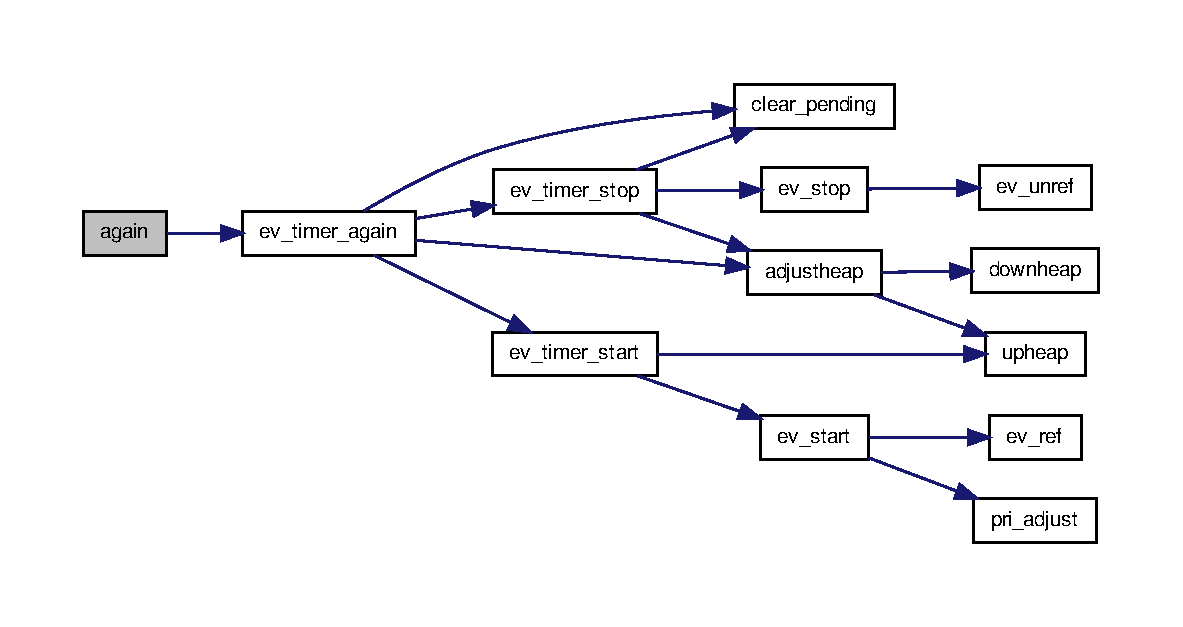
\includegraphics[width=350pt]{namespaceev_ab7c9a87739679053f1cc8d9924997e88_cgraph}
\end{center}
\end{figure}


\hypertarget{namespaceev_af6be39a41980f0e42ffb968bee09889b}{\index{ev@{ev}!async\-\_\-pending@{async\-\_\-pending}}
\index{async\-\_\-pending@{async\-\_\-pending}!ev@{ev}}
\subsubsection[{async\-\_\-pending}]{\setlength{\rightskip}{0pt plus 5cm}bool {\bf ev\-::async\-\_\-pending} (
\begin{DoxyParamCaption}
{}
\end{DoxyParamCaption}
)  throw ()}}\label{namespaceev_af6be39a41980f0e42ffb968bee09889b}


\-Definition at line 801 of file ev++.\-h.

\hypertarget{namespaceev_aea693915baceb9cb7517a52c578a4a94}{\index{ev@{ev}!delay@{delay}}
\index{delay@{delay}!ev@{ev}}
\subsubsection[{delay}]{\setlength{\rightskip}{0pt plus 5cm}void {\bf ev\-::delay} (
\begin{DoxyParamCaption}
\item[{tstamp}]{interval}
\end{DoxyParamCaption}
)  throw ()\hspace{0.3cm}{\ttfamily  \mbox{[}inline\mbox{]}}}}\label{namespaceev_aea693915baceb9cb7517a52c578a4a94}


\-Definition at line 525 of file ev++.\-h.



\-Here is the call graph for this function\-:
\nopagebreak
\begin{figure}[H]
\begin{center}
\leavevmode
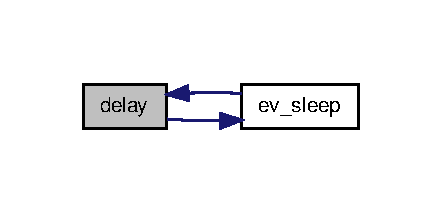
\includegraphics[width=212pt]{namespaceev_aea693915baceb9cb7517a52c578a4a94_cgraph}
\end{center}
\end{figure}




\-Here is the caller graph for this function\-:
\nopagebreak
\begin{figure}[H]
\begin{center}
\leavevmode
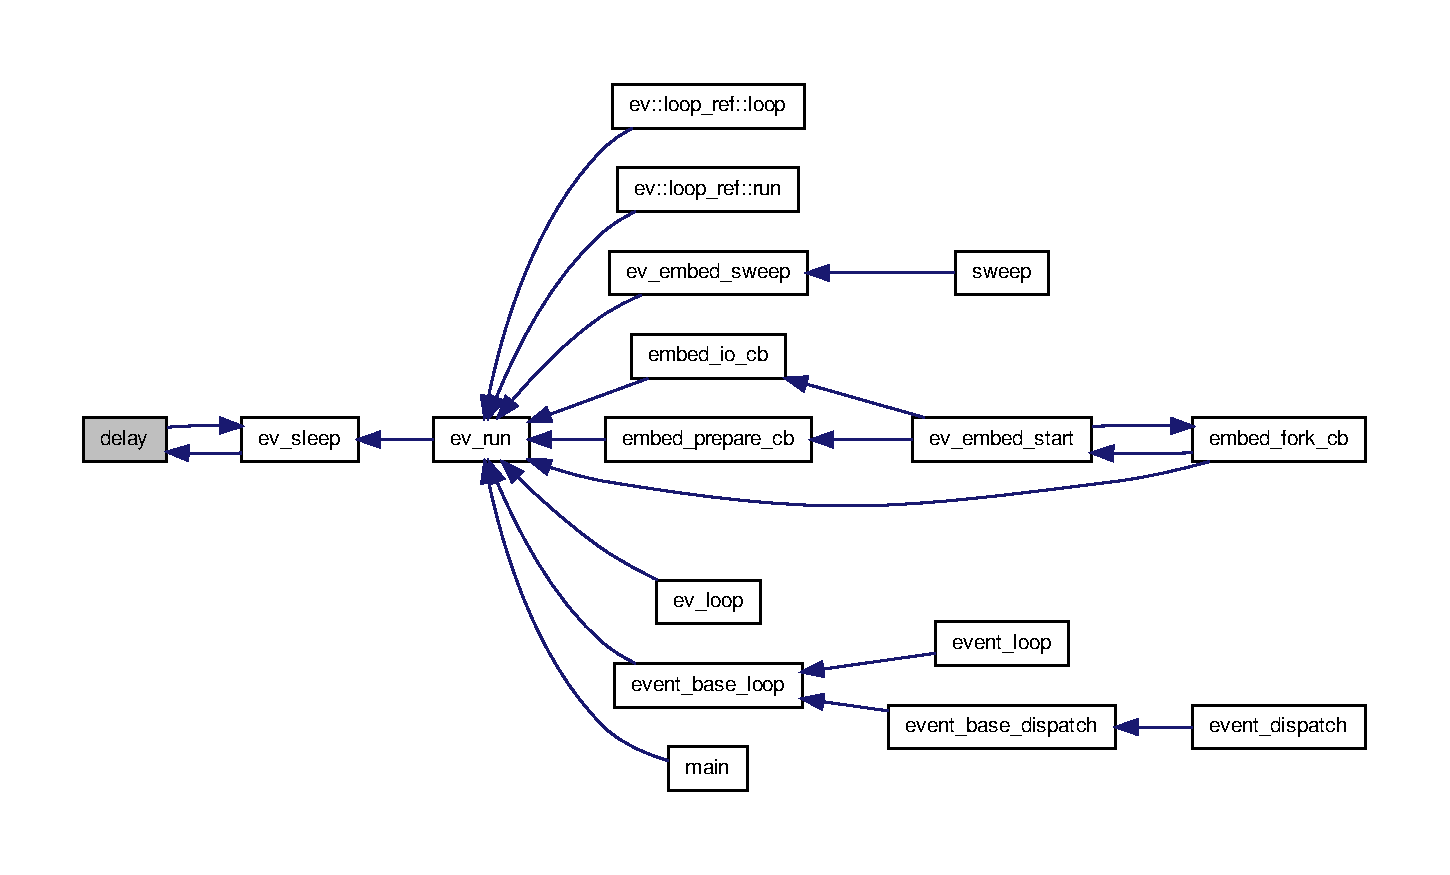
\includegraphics[width=350pt]{namespaceev_aea693915baceb9cb7517a52c578a4a94_icgraph}
\end{center}
\end{figure}


\hypertarget{namespaceev_a0a9dd6a12517dc1d8ece8100eab7b28c}{\index{ev@{ev}!embeddable\-\_\-backends@{embeddable\-\_\-backends}}
\index{embeddable\-\_\-backends@{embeddable\-\_\-backends}!ev@{ev}}
\subsubsection[{embeddable\-\_\-backends}]{\setlength{\rightskip}{0pt plus 5cm}unsigned int {\bf ev\-::embeddable\-\_\-backends} (
\begin{DoxyParamCaption}
{}
\end{DoxyParamCaption}
)  throw ()\hspace{0.3cm}{\ttfamily  \mbox{[}inline\mbox{]}}}}\label{namespaceev_a0a9dd6a12517dc1d8ece8100eab7b28c}


\-Definition at line 550 of file ev++.\-h.



\-Here is the call graph for this function\-:
\nopagebreak
\begin{figure}[H]
\begin{center}
\leavevmode
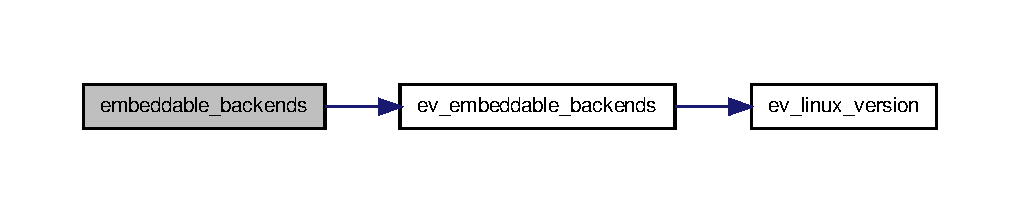
\includegraphics[width=350pt]{namespaceev_a0a9dd6a12517dc1d8ece8100eab7b28c_cgraph}
\end{center}
\end{figure}


\hypertarget{namespaceev_ac0c096b0140f59d5c5abea256f0c75c4}{\index{ev@{ev}!get\-\_\-default\-\_\-loop@{get\-\_\-default\-\_\-loop}}
\index{get\-\_\-default\-\_\-loop@{get\-\_\-default\-\_\-loop}!ev@{ev}}
\subsubsection[{get\-\_\-default\-\_\-loop}]{\setlength{\rightskip}{0pt plus 5cm}{\bf loop\-\_\-ref} {\bf ev\-::get\-\_\-default\-\_\-loop} (
\begin{DoxyParamCaption}
{}
\end{DoxyParamCaption}
)  throw ()\hspace{0.3cm}{\ttfamily  \mbox{[}inline\mbox{]}}}}\label{namespaceev_ac0c096b0140f59d5c5abea256f0c75c4}


\-Definition at line 399 of file ev++.\-h.



\-Here is the call graph for this function\-:
\nopagebreak
\begin{figure}[H]
\begin{center}
\leavevmode
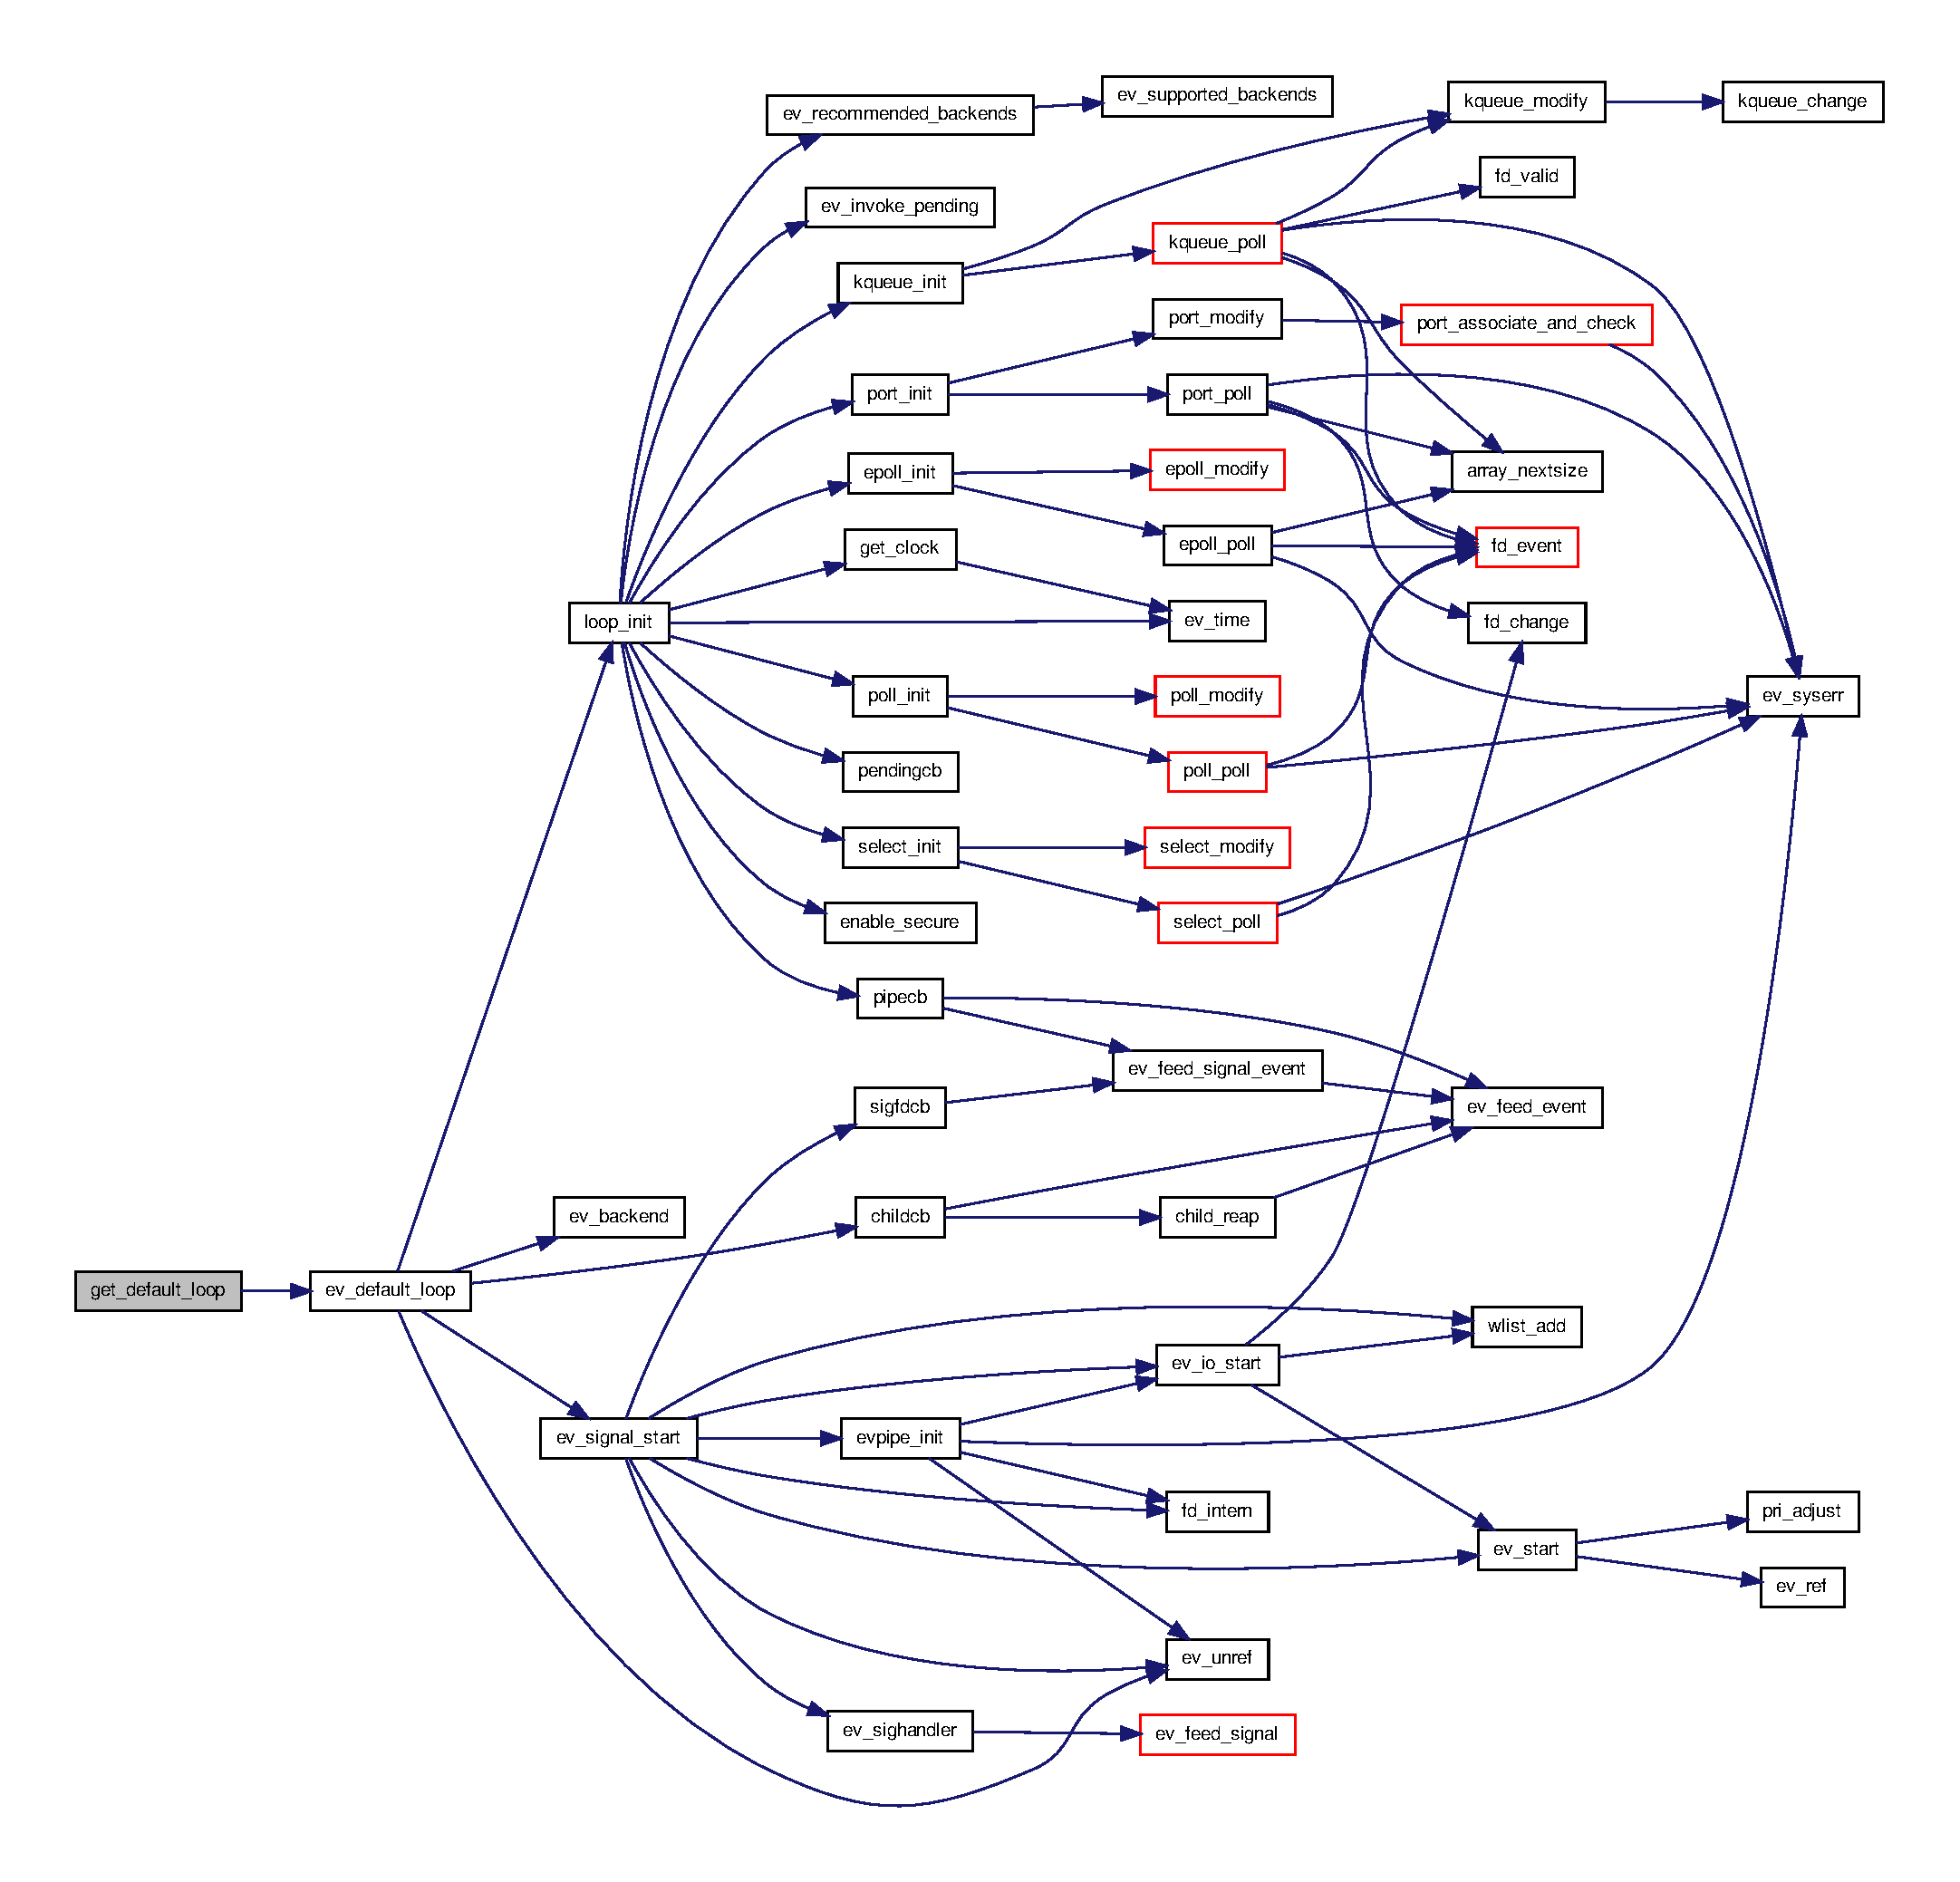
\includegraphics[width=350pt]{namespaceev_ac0c096b0140f59d5c5abea256f0c75c4_cgraph}
\end{center}
\end{figure}


\hypertarget{namespaceev_a260a36d42568d9d1820af7537fc1bae2}{\index{ev@{ev}!now@{now}}
\index{now@{now}!ev@{ev}}
\subsubsection[{now}]{\setlength{\rightskip}{0pt plus 5cm}{\bf tstamp} {\bf ev\-::now} (
\begin{DoxyParamCaption}
\item[{{\bf \-E\-V\-\_\-\-P}}]{}
\end{DoxyParamCaption}
)  throw ()\hspace{0.3cm}{\ttfamily  \mbox{[}inline\mbox{]}}}}\label{namespaceev_a260a36d42568d9d1820af7537fc1bae2}


\-Definition at line 520 of file ev++.\-h.



\-Here is the call graph for this function\-:
\nopagebreak
\begin{figure}[H]
\begin{center}
\leavevmode
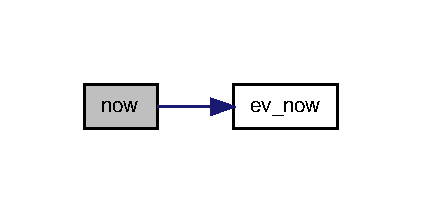
\includegraphics[width=202pt]{namespaceev_a260a36d42568d9d1820af7537fc1bae2_cgraph}
\end{center}
\end{figure}


\hypertarget{namespaceev_a8cb5adc662fb62112386efd00b0af595}{\index{ev@{ev}!recommended\-\_\-backends@{recommended\-\_\-backends}}
\index{recommended\-\_\-backends@{recommended\-\_\-backends}!ev@{ev}}
\subsubsection[{recommended\-\_\-backends}]{\setlength{\rightskip}{0pt plus 5cm}unsigned int {\bf ev\-::recommended\-\_\-backends} (
\begin{DoxyParamCaption}
{}
\end{DoxyParamCaption}
)  throw ()\hspace{0.3cm}{\ttfamily  \mbox{[}inline\mbox{]}}}}\label{namespaceev_a8cb5adc662fb62112386efd00b0af595}


\-Definition at line 545 of file ev++.\-h.



\-Here is the call graph for this function\-:
\nopagebreak
\begin{figure}[H]
\begin{center}
\leavevmode
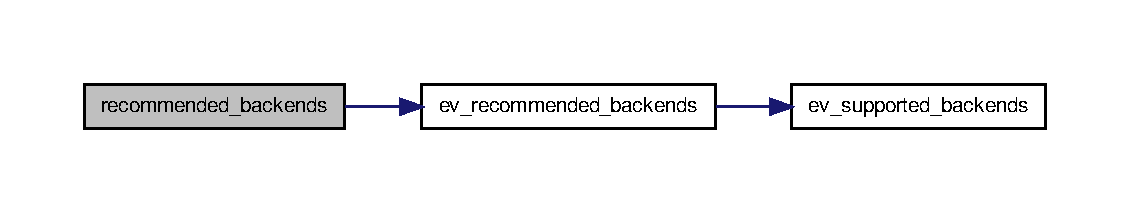
\includegraphics[width=350pt]{namespaceev_a8cb5adc662fb62112386efd00b0af595_cgraph}
\end{center}
\end{figure}


\hypertarget{namespaceev_a5fd889d801efabfac0945b37392e1c80}{\index{ev@{ev}!remaining@{remaining}}
\index{remaining@{remaining}!ev@{ev}}
\subsubsection[{remaining}]{\setlength{\rightskip}{0pt plus 5cm}{\bf ev\-\_\-tstamp} {\bf ev\-::remaining} (
\begin{DoxyParamCaption}
{}
\end{DoxyParamCaption}
)}}\label{namespaceev_a5fd889d801efabfac0945b37392e1c80}


\-Definition at line 658 of file ev++.\-h.



\-Here is the call graph for this function\-:
\nopagebreak
\begin{figure}[H]
\begin{center}
\leavevmode
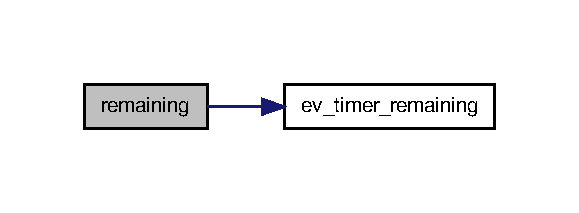
\includegraphics[width=278pt]{namespaceev_a5fd889d801efabfac0945b37392e1c80_cgraph}
\end{center}
\end{figure}


\hypertarget{namespaceev_a28510b06b8f37de1192b841d5eec8d8c}{\index{ev@{ev}!send@{send}}
\index{send@{send}!ev@{ev}}
\subsubsection[{send}]{\setlength{\rightskip}{0pt plus 5cm}void {\bf ev\-::send} (
\begin{DoxyParamCaption}
{}
\end{DoxyParamCaption}
)  throw ()}}\label{namespaceev_a28510b06b8f37de1192b841d5eec8d8c}


\-Definition at line 796 of file ev++.\-h.



\-Here is the call graph for this function\-:
\nopagebreak
\begin{figure}[H]
\begin{center}
\leavevmode
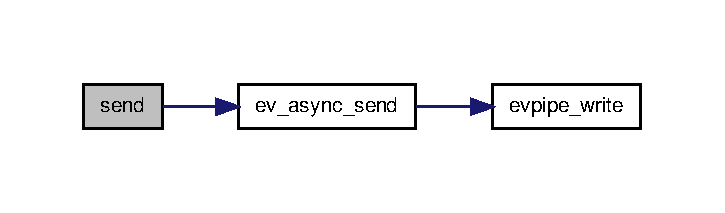
\includegraphics[width=348pt]{namespaceev_a28510b06b8f37de1192b841d5eec8d8c_cgraph}
\end{center}
\end{figure}


\hypertarget{namespaceev_a6b46afd8229a5e1c940c265127857088}{\index{ev@{ev}!set@{set}}
\index{set@{set}!ev@{ev}}
\subsubsection[{set}]{\setlength{\rightskip}{0pt plus 5cm}void {\bf set} (
\begin{DoxyParamCaption}
\item[{int}]{fd, }
\item[{int}]{events = {\ttfamily 0}}
\end{DoxyParamCaption}
)  throw ()}}\label{namespaceev_a6b46afd8229a5e1c940c265127857088}


\-Definition at line 615 of file ev++.\-h.



\-Here is the call graph for this function\-:
\nopagebreak
\begin{figure}[H]
\begin{center}
\leavevmode
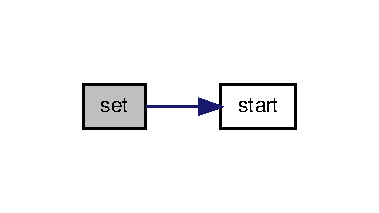
\includegraphics[width=182pt]{namespaceev_a6b46afd8229a5e1c940c265127857088_cgraph}
\end{center}
\end{figure}


\hypertarget{namespaceev_a08ae4b9113645a19793a0b12eea43939}{\index{ev@{ev}!set@{set}}
\index{set@{set}!ev@{ev}}
\subsubsection[{set}]{\setlength{\rightskip}{0pt plus 5cm}void {\bf set} (
\begin{DoxyParamCaption}
\item[{int}]{events}
\end{DoxyParamCaption}
)  throw ()}}\label{namespaceev_a08ae4b9113645a19793a0b12eea43939}


\-Definition at line 623 of file ev++.\-h.



\-Here is the call graph for this function\-:
\nopagebreak
\begin{figure}[H]
\begin{center}
\leavevmode
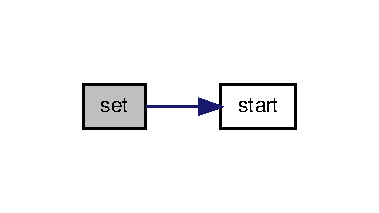
\includegraphics[width=182pt]{namespaceev_a08ae4b9113645a19793a0b12eea43939_cgraph}
\end{center}
\end{figure}


\hypertarget{namespaceev_a62e8d4db09755b6ac44bc00f8a79f947}{\index{ev@{ev}!set@{set}}
\index{set@{set}!ev@{ev}}
\subsubsection[{set}]{\setlength{\rightskip}{0pt plus 5cm}void {\bf set} (
\begin{DoxyParamCaption}
\item[{{\bf ev\-\_\-tstamp}}]{after, }
\item[{{\bf ev\-\_\-tstamp}}]{repeat = {\ttfamily 0.}}
\end{DoxyParamCaption}
)  throw ()}}\label{namespaceev_a62e8d4db09755b6ac44bc00f8a79f947}


\-Definition at line 639 of file ev++.\-h.



\-Here is the call graph for this function\-:
\nopagebreak
\begin{figure}[H]
\begin{center}
\leavevmode
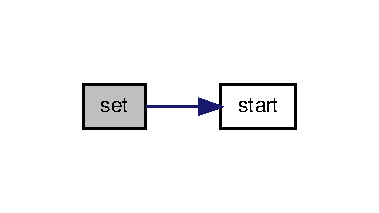
\includegraphics[width=182pt]{namespaceev_a62e8d4db09755b6ac44bc00f8a79f947_cgraph}
\end{center}
\end{figure}


\hypertarget{namespaceev_ac769b7c626617c8c488674381a409ef3}{\index{ev@{ev}!set@{set}}
\index{set@{set}!ev@{ev}}
\subsubsection[{set}]{\setlength{\rightskip}{0pt plus 5cm}void {\bf ev\-::set} (
\begin{DoxyParamCaption}
\item[{const char $\ast$}]{path, }
\item[{{\bf ev\-\_\-tstamp}}]{interval = {\ttfamily 0.}}
\end{DoxyParamCaption}
)  throw ()}}\label{namespaceev_ac769b7c626617c8c488674381a409ef3}


\-Definition at line 725 of file ev++.\-h.



\-Here is the call graph for this function\-:
\nopagebreak
\begin{figure}[H]
\begin{center}
\leavevmode
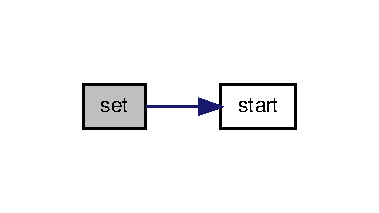
\includegraphics[width=182pt]{namespaceev_ac769b7c626617c8c488674381a409ef3_cgraph}
\end{center}
\end{figure}


\hypertarget{namespaceev_a62bbebcdc34a8056c32d0b1a26026717}{\index{ev@{ev}!set@{set}}
\index{set@{set}!ev@{ev}}
\subsubsection[{set}]{\setlength{\rightskip}{0pt plus 5cm}void {\bf set} (
\begin{DoxyParamCaption}
{}
\end{DoxyParamCaption}
)  throw ()}}\label{namespaceev_a62bbebcdc34a8056c32d0b1a26026717}


\-Definition at line 749 of file ev++.\-h.

\hypertarget{namespaceev_a7ff6e0fbf0cd740f0065b73588dbe7b4}{\index{ev@{ev}!set\-\_\-allocator@{set\-\_\-allocator}}
\index{set\-\_\-allocator@{set\-\_\-allocator}!ev@{ev}}
\subsubsection[{set\-\_\-allocator}]{\setlength{\rightskip}{0pt plus 5cm}void {\bf ev\-::set\-\_\-allocator} (
\begin{DoxyParamCaption}
\item[{void $\ast$}]{$\ast$)(void $\ast$ptr, long size) throw cb(}
\end{DoxyParamCaption}
)  throw ()\hspace{0.3cm}{\ttfamily  \mbox{[}inline\mbox{]}}}}\label{namespaceev_a7ff6e0fbf0cd740f0065b73588dbe7b4}


\-Definition at line 555 of file ev++.\-h.



\-Here is the call graph for this function\-:
\nopagebreak
\begin{figure}[H]
\begin{center}
\leavevmode
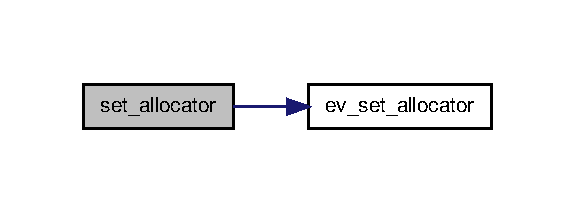
\includegraphics[width=276pt]{namespaceev_a7ff6e0fbf0cd740f0065b73588dbe7b4_cgraph}
\end{center}
\end{figure}


\hypertarget{namespaceev_ad1c1e455ba2c264935c5067bd382cade}{\index{ev@{ev}!set\-\_\-embed@{set\-\_\-embed}}
\index{set\-\_\-embed@{set\-\_\-embed}!ev@{ev}}
\subsubsection[{set\-\_\-embed}]{\setlength{\rightskip}{0pt plus 5cm}void {\bf ev\-::set\-\_\-embed} (
\begin{DoxyParamCaption}
\item[{struct {\bf ev\-\_\-loop} $\ast$}]{embedded\-\_\-loop}
\end{DoxyParamCaption}
)  throw ()}}\label{namespaceev_ad1c1e455ba2c264935c5067bd382cade}


\-Definition at line 767 of file ev++.\-h.



\-Here is the call graph for this function\-:
\nopagebreak
\begin{figure}[H]
\begin{center}
\leavevmode
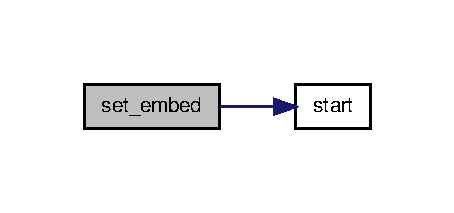
\includegraphics[width=218pt]{namespaceev_ad1c1e455ba2c264935c5067bd382cade_cgraph}
\end{center}
\end{figure}


\hypertarget{namespaceev_abca03339e2d94adc78a0bcf0acf6ccae}{\index{ev@{ev}!set\-\_\-syserr\-\_\-cb@{set\-\_\-syserr\-\_\-cb}}
\index{set\-\_\-syserr\-\_\-cb@{set\-\_\-syserr\-\_\-cb}!ev@{ev}}
\subsubsection[{set\-\_\-syserr\-\_\-cb}]{\setlength{\rightskip}{0pt plus 5cm}void {\bf ev\-::set\-\_\-syserr\-\_\-cb} (
\begin{DoxyParamCaption}
\item[{void($\ast$)(const char $\ast$msg) throw cb()}]{}
\end{DoxyParamCaption}
)  throw ()\hspace{0.3cm}{\ttfamily  \mbox{[}inline\mbox{]}}}}\label{namespaceev_abca03339e2d94adc78a0bcf0acf6ccae}


\-Definition at line 560 of file ev++.\-h.



\-Here is the call graph for this function\-:
\nopagebreak
\begin{figure}[H]
\begin{center}
\leavevmode
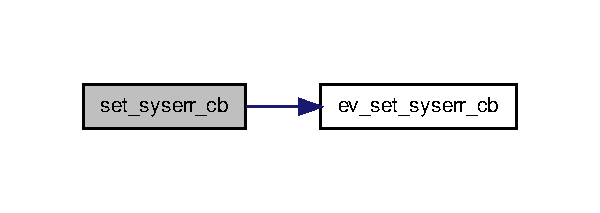
\includegraphics[width=288pt]{namespaceev_abca03339e2d94adc78a0bcf0acf6ccae_cgraph}
\end{center}
\end{figure}


\hypertarget{namespaceev_a1dd5727612e83d2114a052325db53cff}{\index{ev@{ev}!start@{start}}
\index{start@{start}!ev@{ev}}
\subsubsection[{start}]{\setlength{\rightskip}{0pt plus 5cm}void {\bf start} (
\begin{DoxyParamCaption}
\item[{int}]{fd, }
\item[{int}]{events = {\ttfamily 0}}
\end{DoxyParamCaption}
)  throw ()}}\label{namespaceev_a1dd5727612e83d2114a052325db53cff}


\-Definition at line 631 of file ev++.\-h.



\-Here is the caller graph for this function\-:
\nopagebreak
\begin{figure}[H]
\begin{center}
\leavevmode
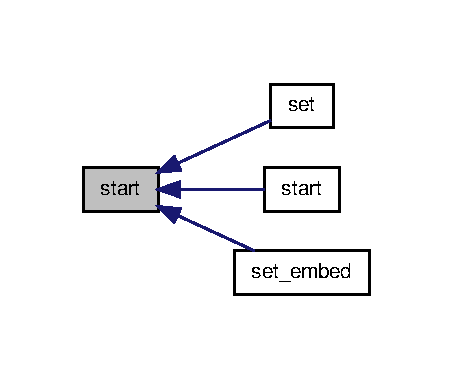
\includegraphics[width=218pt]{namespaceev_a1dd5727612e83d2114a052325db53cff_icgraph}
\end{center}
\end{figure}


\hypertarget{namespaceev_a8c79d5364cc6a464e5e43978894e2e65}{\index{ev@{ev}!start@{start}}
\index{start@{start}!ev@{ev}}
\subsubsection[{start}]{\setlength{\rightskip}{0pt plus 5cm}void {\bf start} (
\begin{DoxyParamCaption}
\item[{{\bf ev\-\_\-tstamp}}]{after, }
\item[{{\bf ev\-\_\-tstamp}}]{repeat = {\ttfamily 0.}}
\end{DoxyParamCaption}
)  throw ()}}\label{namespaceev_a8c79d5364cc6a464e5e43978894e2e65}


\-Definition at line 647 of file ev++.\-h.



\-Here is the call graph for this function\-:
\nopagebreak
\begin{figure}[H]
\begin{center}
\leavevmode
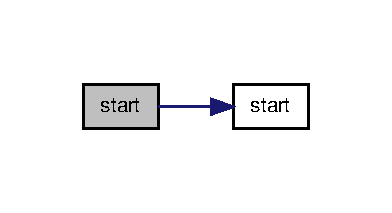
\includegraphics[width=188pt]{namespaceev_a8c79d5364cc6a464e5e43978894e2e65_cgraph}
\end{center}
\end{figure}


\hypertarget{namespaceev_adc6909ad912a1dcadd1c6057bb22abd2}{\index{ev@{ev}!start@{start}}
\index{start@{start}!ev@{ev}}
\subsubsection[{start}]{\setlength{\rightskip}{0pt plus 5cm}void {\bf ev\-::start} (
\begin{DoxyParamCaption}
\item[{int}]{signum}
\end{DoxyParamCaption}
)  throw ()}}\label{namespaceev_adc6909ad912a1dcadd1c6057bb22abd2}


\-Definition at line 697 of file ev++.\-h.



\-Here is the call graph for this function\-:
\nopagebreak
\begin{figure}[H]
\begin{center}
\leavevmode
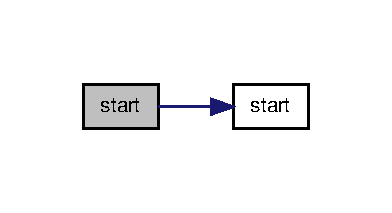
\includegraphics[width=188pt]{namespaceev_adc6909ad912a1dcadd1c6057bb22abd2_cgraph}
\end{center}
\end{figure}


\hypertarget{namespaceev_ad301ec74ae585578be337d2cd1c4c306}{\index{ev@{ev}!start@{start}}
\index{start@{start}!ev@{ev}}
\subsubsection[{start}]{\setlength{\rightskip}{0pt plus 5cm}void {\bf ev\-::start} (
\begin{DoxyParamCaption}
\item[{const char $\ast$}]{path, }
\item[{{\bf ev\-\_\-tstamp}}]{interval = {\ttfamily 0.}}
\end{DoxyParamCaption}
)  throw ()}}\label{namespaceev_ad301ec74ae585578be337d2cd1c4c306}


\-Definition at line 733 of file ev++.\-h.



\-Here is the call graph for this function\-:
\nopagebreak
\begin{figure}[H]
\begin{center}
\leavevmode
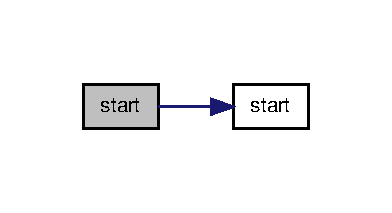
\includegraphics[width=188pt]{namespaceev_ad301ec74ae585578be337d2cd1c4c306_cgraph}
\end{center}
\end{figure}


\hypertarget{namespaceev_a6a90facb9d608bdabb83b7cb4416b110}{\index{ev@{ev}!start@{start}}
\index{start@{start}!ev@{ev}}
\subsubsection[{start}]{\setlength{\rightskip}{0pt plus 5cm}void {\bf ev\-::start} (
\begin{DoxyParamCaption}
\item[{struct {\bf ev\-\_\-loop} $\ast$}]{embedded\-\_\-loop}
\end{DoxyParamCaption}
)  throw ()}}\label{namespaceev_a6a90facb9d608bdabb83b7cb4416b110}


\-Definition at line 775 of file ev++.\-h.



\-Here is the call graph for this function\-:
\nopagebreak
\begin{figure}[H]
\begin{center}
\leavevmode
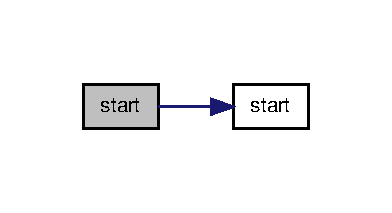
\includegraphics[width=188pt]{namespaceev_a6a90facb9d608bdabb83b7cb4416b110_cgraph}
\end{center}
\end{figure}


\hypertarget{namespaceev_ae3ffb75868e8c2922a0f4a2f67593093}{\index{ev@{ev}!supported\-\_\-backends@{supported\-\_\-backends}}
\index{supported\-\_\-backends@{supported\-\_\-backends}!ev@{ev}}
\subsubsection[{supported\-\_\-backends}]{\setlength{\rightskip}{0pt plus 5cm}unsigned int {\bf ev\-::supported\-\_\-backends} (
\begin{DoxyParamCaption}
{}
\end{DoxyParamCaption}
)  throw ()\hspace{0.3cm}{\ttfamily  \mbox{[}inline\mbox{]}}}}\label{namespaceev_ae3ffb75868e8c2922a0f4a2f67593093}


\-Definition at line 540 of file ev++.\-h.



\-Here is the call graph for this function\-:
\nopagebreak
\begin{figure}[H]
\begin{center}
\leavevmode
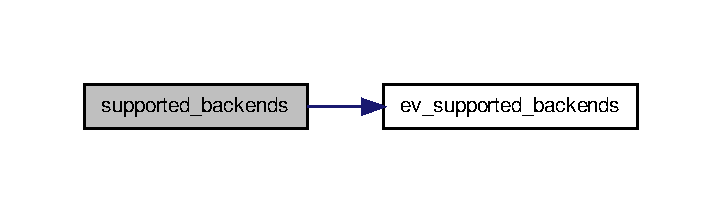
\includegraphics[width=346pt]{namespaceev_ae3ffb75868e8c2922a0f4a2f67593093_cgraph}
\end{center}
\end{figure}


\hypertarget{namespaceev_adb7cfbaaf2a233e8b17711e118c8987a}{\index{ev@{ev}!sweep@{sweep}}
\index{sweep@{sweep}!ev@{ev}}
\subsubsection[{sweep}]{\setlength{\rightskip}{0pt plus 5cm}void {\bf ev\-::sweep} (
\begin{DoxyParamCaption}
{}
\end{DoxyParamCaption}
)}}\label{namespaceev_adb7cfbaaf2a233e8b17711e118c8987a}


\-Definition at line 781 of file ev++.\-h.



\-Here is the call graph for this function\-:
\nopagebreak
\begin{figure}[H]
\begin{center}
\leavevmode
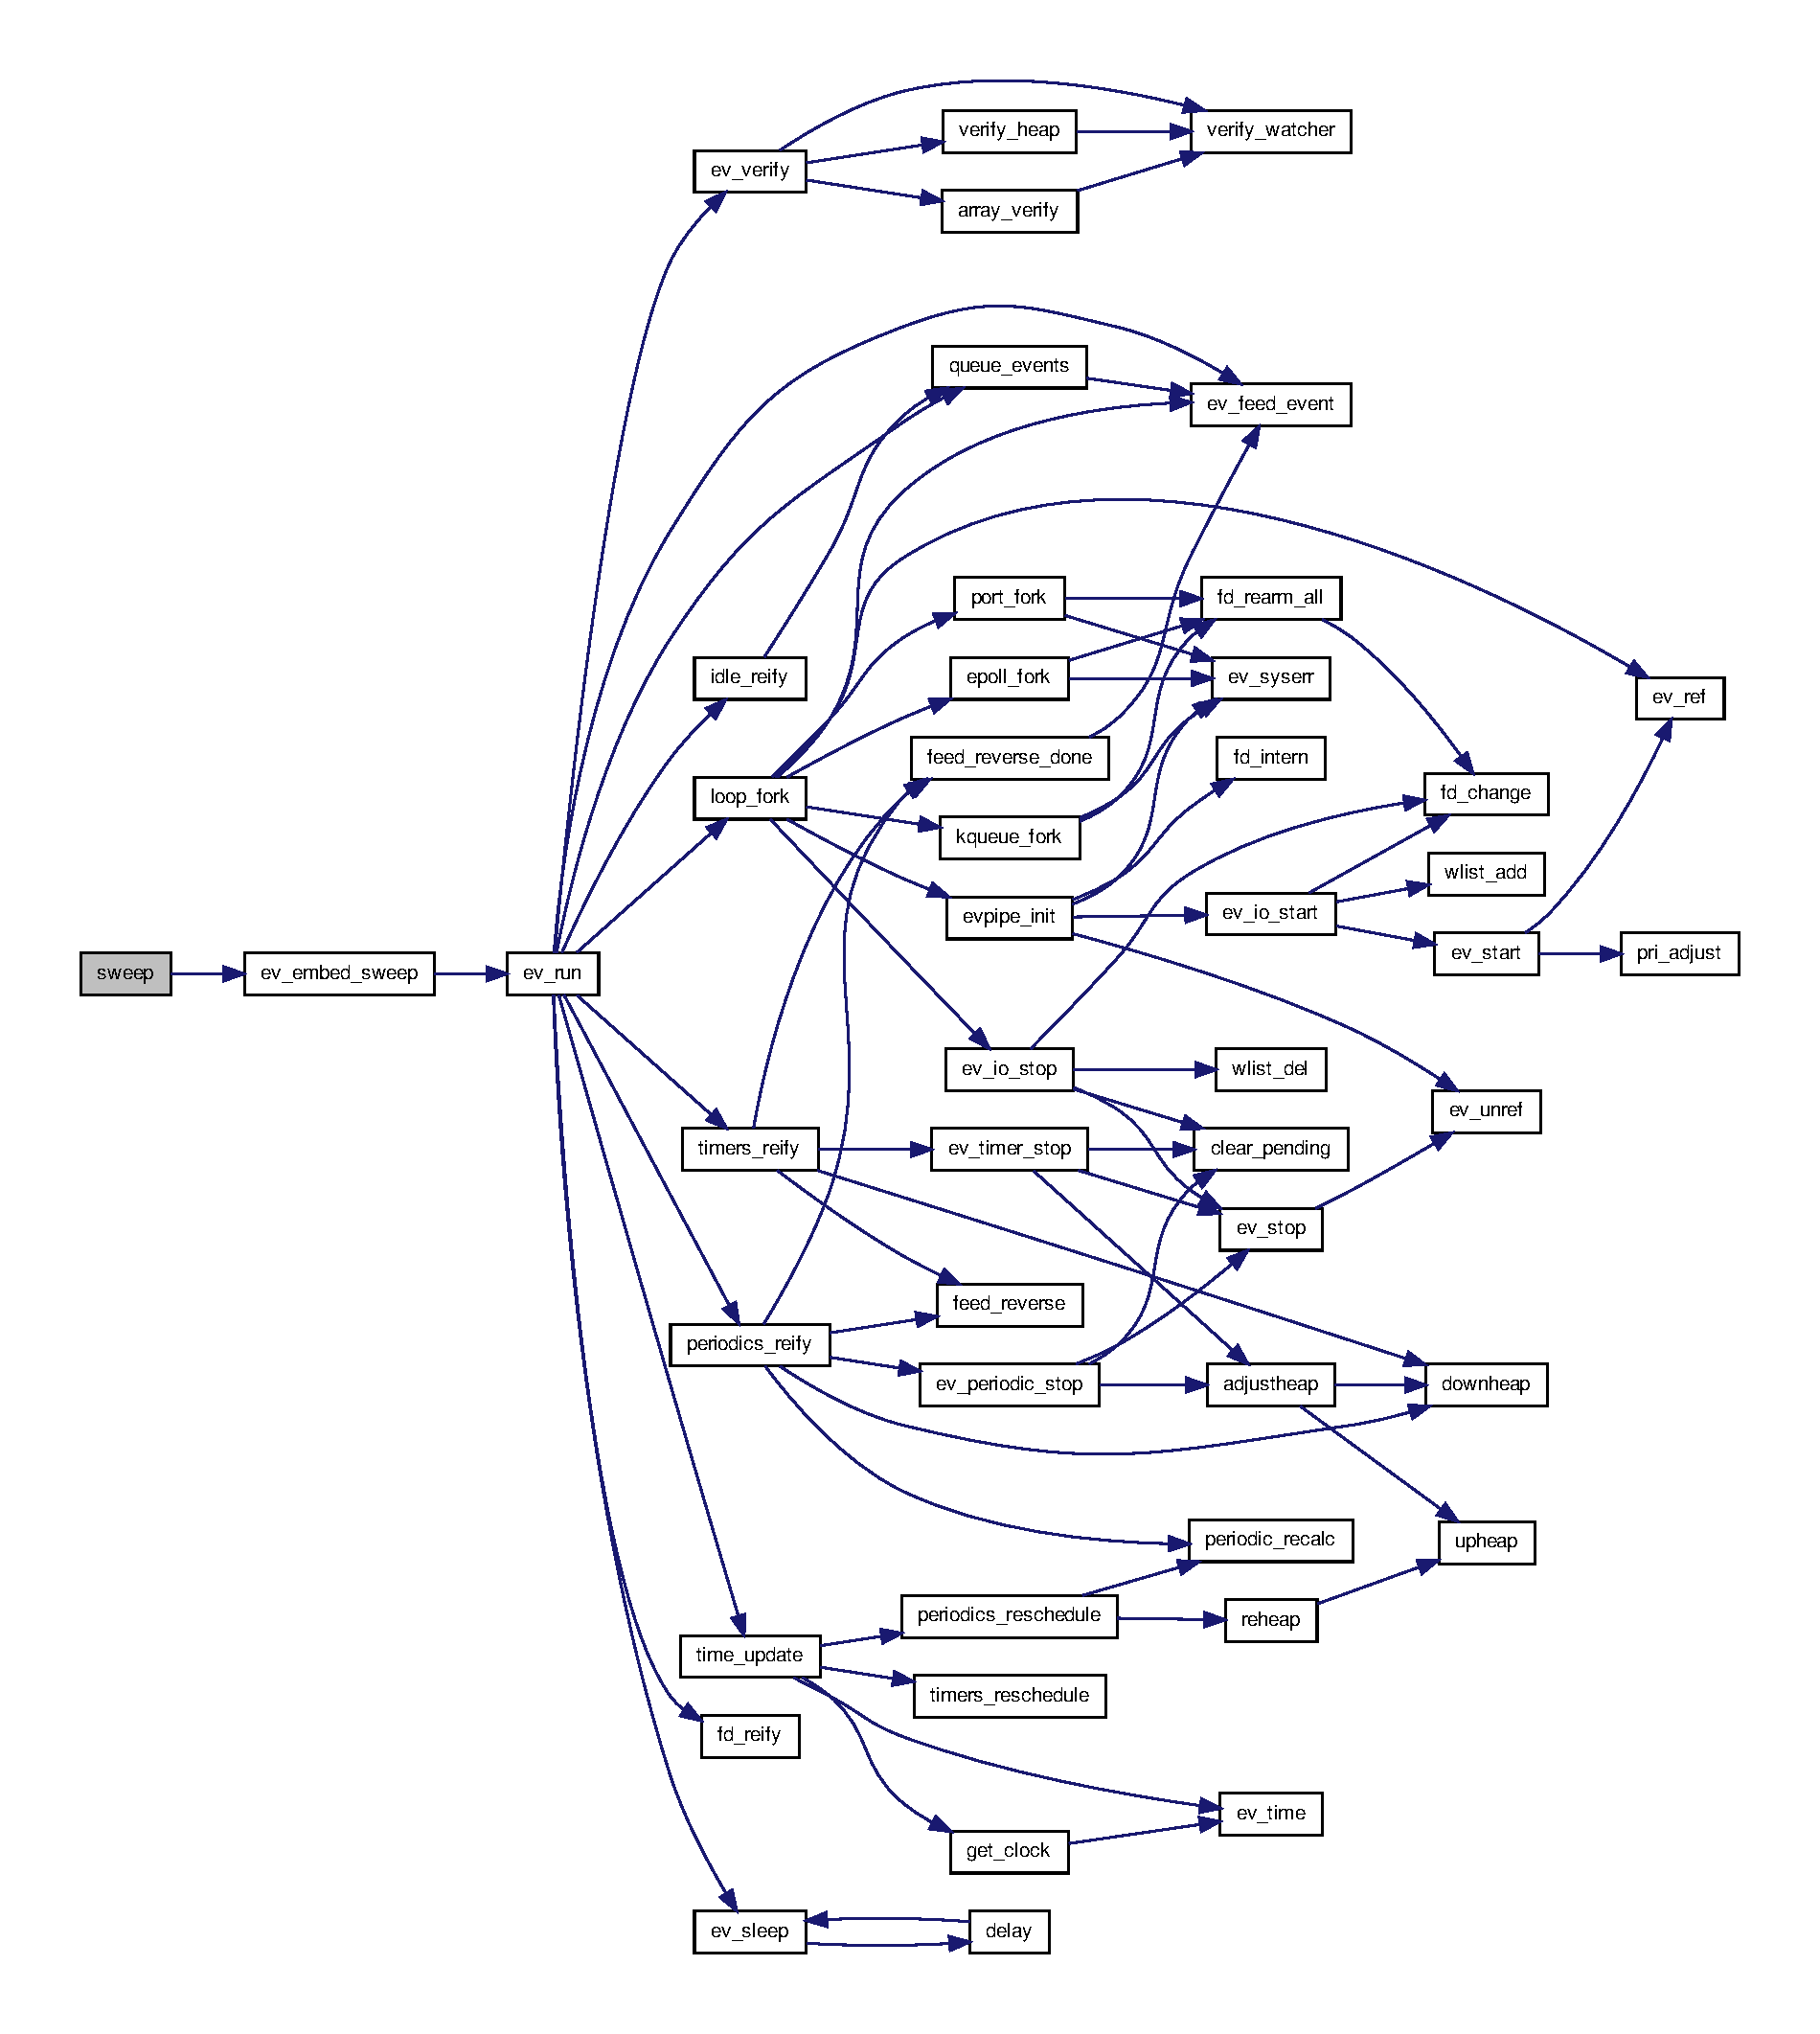
\includegraphics[width=350pt]{namespaceev_adb7cfbaaf2a233e8b17711e118c8987a_cgraph}
\end{center}
\end{figure}


\hypertarget{namespaceev_a5bb641560ccc45a778d39c887887c354}{\index{ev@{ev}!update@{update}}
\index{update@{update}!ev@{ev}}
\subsubsection[{update}]{\setlength{\rightskip}{0pt plus 5cm}void {\bf ev\-::update} (
\begin{DoxyParamCaption}
{}
\end{DoxyParamCaption}
)  throw ()}}\label{namespaceev_a5bb641560ccc45a778d39c887887c354}


\-Definition at line 740 of file ev++.\-h.



\-Here is the call graph for this function\-:
\nopagebreak
\begin{figure}[H]
\begin{center}
\leavevmode
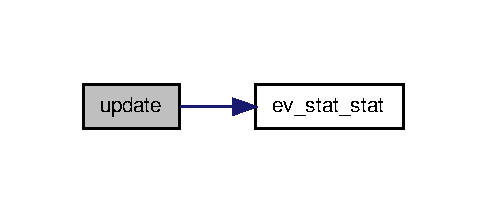
\includegraphics[width=234pt]{namespaceev_a5bb641560ccc45a778d39c887887c354_cgraph}
\end{center}
\end{figure}


\hypertarget{namespaceev_a0d3917d61c37bb24db1d864e2ac4552f}{\index{ev@{ev}!version\-\_\-major@{version\-\_\-major}}
\index{version\-\_\-major@{version\-\_\-major}!ev@{ev}}
\subsubsection[{version\-\_\-major}]{\setlength{\rightskip}{0pt plus 5cm}int {\bf ev\-::version\-\_\-major} (
\begin{DoxyParamCaption}
{}
\end{DoxyParamCaption}
)  throw ()\hspace{0.3cm}{\ttfamily  \mbox{[}inline\mbox{]}}}}\label{namespaceev_a0d3917d61c37bb24db1d864e2ac4552f}


\-Definition at line 530 of file ev++.\-h.



\-Here is the call graph for this function\-:
\nopagebreak
\begin{figure}[H]
\begin{center}
\leavevmode
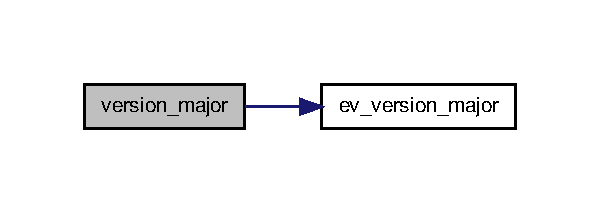
\includegraphics[width=288pt]{namespaceev_a0d3917d61c37bb24db1d864e2ac4552f_cgraph}
\end{center}
\end{figure}


\hypertarget{namespaceev_abfc4ac781668b20171841d8dda0317a0}{\index{ev@{ev}!version\-\_\-minor@{version\-\_\-minor}}
\index{version\-\_\-minor@{version\-\_\-minor}!ev@{ev}}
\subsubsection[{version\-\_\-minor}]{\setlength{\rightskip}{0pt plus 5cm}int {\bf ev\-::version\-\_\-minor} (
\begin{DoxyParamCaption}
{}
\end{DoxyParamCaption}
)  throw ()\hspace{0.3cm}{\ttfamily  \mbox{[}inline\mbox{]}}}}\label{namespaceev_abfc4ac781668b20171841d8dda0317a0}


\-Definition at line 535 of file ev++.\-h.



\-Here is the call graph for this function\-:
\nopagebreak
\begin{figure}[H]
\begin{center}
\leavevmode
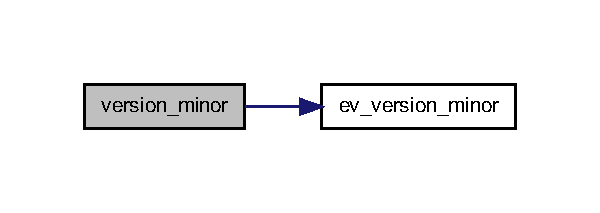
\includegraphics[width=288pt]{namespaceev_abfc4ac781668b20171841d8dda0317a0_cgraph}
\end{center}
\end{figure}



\chapter{\-Data \-Structure \-Documentation}
\hypertarget{struct_a_n_f_d}{\section{\-A\-N\-F\-D \-Struct \-Reference}
\label{struct_a_n_f_d}\index{\-A\-N\-F\-D@{\-A\-N\-F\-D}}
}


\-Collaboration diagram for \-A\-N\-F\-D\-:
\nopagebreak
\begin{figure}[H]
\begin{center}
\leavevmode
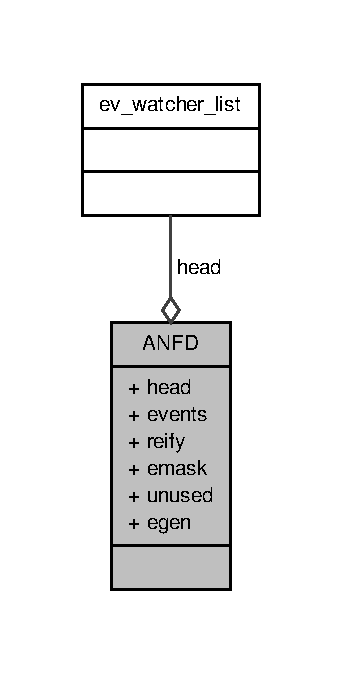
\includegraphics[width=164pt]{struct_a_n_f_d__coll__graph}
\end{center}
\end{figure}
\subsection*{\-Data \-Fields}
\begin{DoxyCompactItemize}
\item 
\hyperlink{ev_8c_a0828ab15b964af31c49b160d210ca60b}{\-W\-L} \hyperlink{struct_a_n_f_d_adfe98a723723ae76746a9a793f2bd862}{head}
\item 
unsigned char \hyperlink{struct_a_n_f_d_a6afb9ac2ccc07c1c5c4adb0ba40fe303}{events}
\item 
unsigned char \hyperlink{struct_a_n_f_d_a9f83e28e70418fa3d19299c0a6562dc9}{reify}
\item 
unsigned char \hyperlink{struct_a_n_f_d_acfe97a2a9e6eb619c00317e774f11b76}{emask}
\item 
unsigned char \hyperlink{struct_a_n_f_d_ad10d012877d07ca3b2e818f11bf97a0f}{unused}
\item 
unsigned int \hyperlink{struct_a_n_f_d_ae3d672a0de46c808d2bae5a187b54478}{egen}
\end{DoxyCompactItemize}


\subsection{\-Detailed \-Description}


\-Definition at line 1559 of file ev.\-c.



\subsection{\-Field \-Documentation}
\hypertarget{struct_a_n_f_d_ae3d672a0de46c808d2bae5a187b54478}{\index{\-A\-N\-F\-D@{\-A\-N\-F\-D}!egen@{egen}}
\index{egen@{egen}!ANFD@{\-A\-N\-F\-D}}
\subsubsection[{egen}]{\setlength{\rightskip}{0pt plus 5cm}unsigned int {\bf egen}}}\label{struct_a_n_f_d_ae3d672a0de46c808d2bae5a187b54478}


\-Definition at line 1567 of file ev.\-c.

\hypertarget{struct_a_n_f_d_acfe97a2a9e6eb619c00317e774f11b76}{\index{\-A\-N\-F\-D@{\-A\-N\-F\-D}!emask@{emask}}
\index{emask@{emask}!ANFD@{\-A\-N\-F\-D}}
\subsubsection[{emask}]{\setlength{\rightskip}{0pt plus 5cm}unsigned char {\bf emask}}}\label{struct_a_n_f_d_acfe97a2a9e6eb619c00317e774f11b76}


\-Definition at line 1564 of file ev.\-c.

\hypertarget{struct_a_n_f_d_a6afb9ac2ccc07c1c5c4adb0ba40fe303}{\index{\-A\-N\-F\-D@{\-A\-N\-F\-D}!events@{events}}
\index{events@{events}!ANFD@{\-A\-N\-F\-D}}
\subsubsection[{events}]{\setlength{\rightskip}{0pt plus 5cm}unsigned char {\bf events}}}\label{struct_a_n_f_d_a6afb9ac2ccc07c1c5c4adb0ba40fe303}


\-Definition at line 1562 of file ev.\-c.

\hypertarget{struct_a_n_f_d_adfe98a723723ae76746a9a793f2bd862}{\index{\-A\-N\-F\-D@{\-A\-N\-F\-D}!head@{head}}
\index{head@{head}!ANFD@{\-A\-N\-F\-D}}
\subsubsection[{head}]{\setlength{\rightskip}{0pt plus 5cm}{\bf \-W\-L} {\bf head}}}\label{struct_a_n_f_d_adfe98a723723ae76746a9a793f2bd862}


\-Definition at line 1561 of file ev.\-c.

\hypertarget{struct_a_n_f_d_a9f83e28e70418fa3d19299c0a6562dc9}{\index{\-A\-N\-F\-D@{\-A\-N\-F\-D}!reify@{reify}}
\index{reify@{reify}!ANFD@{\-A\-N\-F\-D}}
\subsubsection[{reify}]{\setlength{\rightskip}{0pt plus 5cm}unsigned char {\bf reify}}}\label{struct_a_n_f_d_a9f83e28e70418fa3d19299c0a6562dc9}


\-Definition at line 1563 of file ev.\-c.

\hypertarget{struct_a_n_f_d_ad10d012877d07ca3b2e818f11bf97a0f}{\index{\-A\-N\-F\-D@{\-A\-N\-F\-D}!unused@{unused}}
\index{unused@{unused}!ANFD@{\-A\-N\-F\-D}}
\subsubsection[{unused}]{\setlength{\rightskip}{0pt plus 5cm}unsigned char {\bf unused}}}\label{struct_a_n_f_d_ad10d012877d07ca3b2e818f11bf97a0f}


\-Definition at line 1565 of file ev.\-c.



\-The documentation for this struct was generated from the following file\-:\begin{DoxyCompactItemize}
\item 
/home/jaymiao/workstation/github/libev-\/4.\-19/\hyperlink{ev_8c}{ev.\-c}\end{DoxyCompactItemize}

\hypertarget{struct_a_n_h_e}{\section{\-A\-N\-H\-E \-Struct \-Reference}
\label{struct_a_n_h_e}\index{\-A\-N\-H\-E@{\-A\-N\-H\-E}}
}


\-Collaboration diagram for \-A\-N\-H\-E\-:
\nopagebreak
\begin{figure}[H]
\begin{center}
\leavevmode
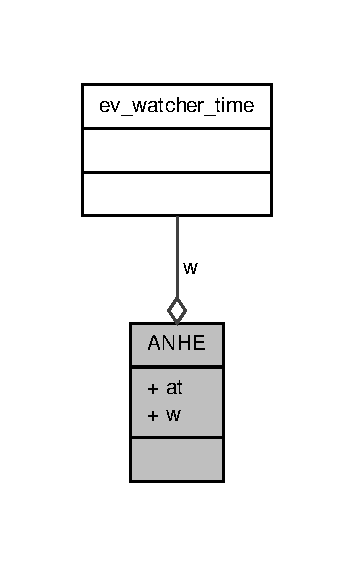
\includegraphics[width=170pt]{struct_a_n_h_e__coll__graph}
\end{center}
\end{figure}
\subsection*{\-Data \-Fields}
\begin{DoxyCompactItemize}
\item 
\hyperlink{ev_8h_add71e34ce2b04bbf7eb6f31a850814e8}{ev\-\_\-tstamp} \hyperlink{struct_a_n_h_e_a6160b512f37d4b32af5c7bad0c700b93}{at}
\item 
\hyperlink{ev_8c_a1634bbf7bbc46bf192d977104e39b6e1}{\-W\-T} \hyperlink{struct_a_n_h_e_af273b2db3bb121b1f6bd0ef8eff603e6}{w}
\end{DoxyCompactItemize}


\subsection{\-Detailed \-Description}


\-Definition at line 1595 of file ev.\-c.



\subsection{\-Field \-Documentation}
\hypertarget{struct_a_n_h_e_a6160b512f37d4b32af5c7bad0c700b93}{\index{\-A\-N\-H\-E@{\-A\-N\-H\-E}!at@{at}}
\index{at@{at}!ANHE@{\-A\-N\-H\-E}}
\subsubsection[{at}]{\setlength{\rightskip}{0pt plus 5cm}{\bf ev\-\_\-tstamp} {\bf at}}}\label{struct_a_n_h_e_a6160b512f37d4b32af5c7bad0c700b93}


\-Definition at line 1596 of file ev.\-c.

\hypertarget{struct_a_n_h_e_af273b2db3bb121b1f6bd0ef8eff603e6}{\index{\-A\-N\-H\-E@{\-A\-N\-H\-E}!w@{w}}
\index{w@{w}!ANHE@{\-A\-N\-H\-E}}
\subsubsection[{w}]{\setlength{\rightskip}{0pt plus 5cm}{\bf \-W\-T} {\bf w}}}\label{struct_a_n_h_e_af273b2db3bb121b1f6bd0ef8eff603e6}


\-Definition at line 1597 of file ev.\-c.



\-The documentation for this struct was generated from the following file\-:\begin{DoxyCompactItemize}
\item 
/home/jaymiao/workstation/github/libev-\/4.\-19/\hyperlink{ev_8c}{ev.\-c}\end{DoxyCompactItemize}

\hypertarget{struct_a_n_p_e_n_d_i_n_g}{\section{\-A\-N\-P\-E\-N\-D\-I\-N\-G \-Struct \-Reference}
\label{struct_a_n_p_e_n_d_i_n_g}\index{\-A\-N\-P\-E\-N\-D\-I\-N\-G@{\-A\-N\-P\-E\-N\-D\-I\-N\-G}}
}


\-Collaboration diagram for \-A\-N\-P\-E\-N\-D\-I\-N\-G\-:
\nopagebreak
\begin{figure}[H]
\begin{center}
\leavevmode
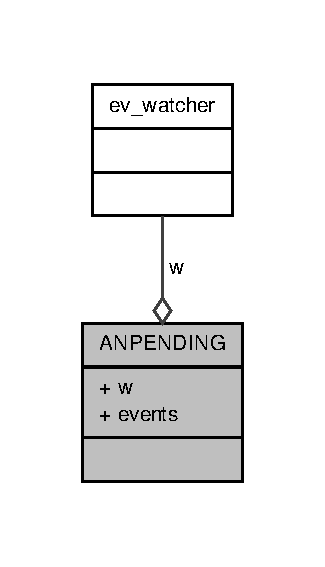
\includegraphics[width=156pt]{struct_a_n_p_e_n_d_i_n_g__coll__graph}
\end{center}
\end{figure}
\subsection*{\-Data \-Fields}
\begin{DoxyCompactItemize}
\item 
\hyperlink{ev_8c_a1d5a98f4500d54b812947ada8c7d517f}{\-W} \hyperlink{struct_a_n_p_e_n_d_i_n_g_aa2a9fd41c12285551bc8b6554950bd61}{w}
\item 
int \hyperlink{struct_a_n_p_e_n_d_i_n_g_a81a8a3a775bf2b769ce2a0f687a44c9f}{events}
\end{DoxyCompactItemize}


\subsection{\-Detailed \-Description}


\-Definition at line 1578 of file ev.\-c.



\subsection{\-Field \-Documentation}
\hypertarget{struct_a_n_p_e_n_d_i_n_g_a81a8a3a775bf2b769ce2a0f687a44c9f}{\index{\-A\-N\-P\-E\-N\-D\-I\-N\-G@{\-A\-N\-P\-E\-N\-D\-I\-N\-G}!events@{events}}
\index{events@{events}!ANPENDING@{\-A\-N\-P\-E\-N\-D\-I\-N\-G}}
\subsubsection[{events}]{\setlength{\rightskip}{0pt plus 5cm}int {\bf events}}}\label{struct_a_n_p_e_n_d_i_n_g_a81a8a3a775bf2b769ce2a0f687a44c9f}


\-Definition at line 1581 of file ev.\-c.

\hypertarget{struct_a_n_p_e_n_d_i_n_g_aa2a9fd41c12285551bc8b6554950bd61}{\index{\-A\-N\-P\-E\-N\-D\-I\-N\-G@{\-A\-N\-P\-E\-N\-D\-I\-N\-G}!w@{w}}
\index{w@{w}!ANPENDING@{\-A\-N\-P\-E\-N\-D\-I\-N\-G}}
\subsubsection[{w}]{\setlength{\rightskip}{0pt plus 5cm}{\bf \-W} {\bf w}}}\label{struct_a_n_p_e_n_d_i_n_g_aa2a9fd41c12285551bc8b6554950bd61}


\-Definition at line 1580 of file ev.\-c.



\-The documentation for this struct was generated from the following file\-:\begin{DoxyCompactItemize}
\item 
/home/jaymiao/workstation/github/libev-\/4.\-19/\hyperlink{ev_8c}{ev.\-c}\end{DoxyCompactItemize}

\hypertarget{struct_a_n_s_i_g}{\section{\-A\-N\-S\-I\-G \-Struct \-Reference}
\label{struct_a_n_s_i_g}\index{\-A\-N\-S\-I\-G@{\-A\-N\-S\-I\-G}}
}


\-Collaboration diagram for \-A\-N\-S\-I\-G\-:
\nopagebreak
\begin{figure}[H]
\begin{center}
\leavevmode
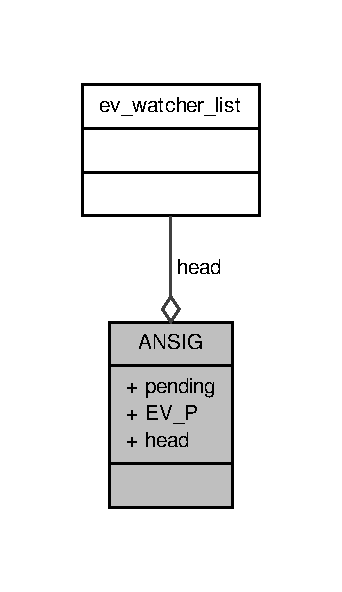
\includegraphics[width=164pt]{struct_a_n_s_i_g__coll__graph}
\end{center}
\end{figure}
\subsection*{\-Data \-Fields}
\begin{DoxyCompactItemize}
\item 
\-E\-V\-\_\-\-A\-T\-O\-M\-I\-C\-\_\-\-T \hyperlink{struct_a_n_s_i_g_a63e6db022c8882b3af1efcdd00e5dbd4}{pending}
\item 
\hyperlink{struct_a_n_s_i_g_a2ac4652fbc25ea6c30d7158cfe5e7698}{\-E\-V\-\_\-\-P}
\item 
\hyperlink{ev_8c_a0828ab15b964af31c49b160d210ca60b}{\-W\-L} \hyperlink{struct_a_n_s_i_g_adfe98a723723ae76746a9a793f2bd862}{head}
\end{DoxyCompactItemize}


\subsection{\-Detailed \-Description}


\-Definition at line 2166 of file ev.\-c.



\subsection{\-Field \-Documentation}
\hypertarget{struct_a_n_s_i_g_a2ac4652fbc25ea6c30d7158cfe5e7698}{\index{\-A\-N\-S\-I\-G@{\-A\-N\-S\-I\-G}!\-E\-V\-\_\-\-P@{\-E\-V\-\_\-\-P}}
\index{\-E\-V\-\_\-\-P@{\-E\-V\-\_\-\-P}!ANSIG@{\-A\-N\-S\-I\-G}}
\subsubsection[{\-E\-V\-\_\-\-P}]{\setlength{\rightskip}{0pt plus 5cm}{\bf \-E\-V\-\_\-\-P}}}\label{struct_a_n_s_i_g_a2ac4652fbc25ea6c30d7158cfe5e7698}


\-Definition at line 2170 of file ev.\-c.

\hypertarget{struct_a_n_s_i_g_adfe98a723723ae76746a9a793f2bd862}{\index{\-A\-N\-S\-I\-G@{\-A\-N\-S\-I\-G}!head@{head}}
\index{head@{head}!ANSIG@{\-A\-N\-S\-I\-G}}
\subsubsection[{head}]{\setlength{\rightskip}{0pt plus 5cm}{\bf \-W\-L} {\bf head}}}\label{struct_a_n_s_i_g_adfe98a723723ae76746a9a793f2bd862}


\-Definition at line 2172 of file ev.\-c.

\hypertarget{struct_a_n_s_i_g_a63e6db022c8882b3af1efcdd00e5dbd4}{\index{\-A\-N\-S\-I\-G@{\-A\-N\-S\-I\-G}!pending@{pending}}
\index{pending@{pending}!ANSIG@{\-A\-N\-S\-I\-G}}
\subsubsection[{pending}]{\setlength{\rightskip}{0pt plus 5cm}\-E\-V\-\_\-\-A\-T\-O\-M\-I\-C\-\_\-\-T {\bf pending}}}\label{struct_a_n_s_i_g_a63e6db022c8882b3af1efcdd00e5dbd4}


\-Definition at line 2168 of file ev.\-c.



\-The documentation for this struct was generated from the following file\-:\begin{DoxyCompactItemize}
\item 
/home/jaymiao/workstation/github/libev-\/4.\-19/\hyperlink{ev_8c}{ev.\-c}\end{DoxyCompactItemize}

\hypertarget{structev_1_1bad__loop}{\section{bad\-\_\-loop \-Struct \-Reference}
\label{structev_1_1bad__loop}\index{bad\-\_\-loop@{bad\-\_\-loop}}
}


{\ttfamily \#include $<$ev++.\-h$>$}

\subsection*{\-Public \-Member \-Functions}
\begin{DoxyCompactItemize}
\item 
\hyperlink{structev_1_1bad__loop_a93f99cac6c15f7dd45698c8552f487f2}{bad\-\_\-loop} ()
\end{DoxyCompactItemize}


\subsection{\-Detailed \-Description}


\-Definition at line 114 of file ev++.\-h.



\subsection{\-Constructor \& \-Destructor \-Documentation}
\hypertarget{structev_1_1bad__loop_a93f99cac6c15f7dd45698c8552f487f2}{\index{ev\-::bad\-\_\-loop@{ev\-::bad\-\_\-loop}!bad\-\_\-loop@{bad\-\_\-loop}}
\index{bad\-\_\-loop@{bad\-\_\-loop}!ev::bad_loop@{ev\-::bad\-\_\-loop}}
\subsubsection[{bad\-\_\-loop}]{\setlength{\rightskip}{0pt plus 5cm}{\bf bad\-\_\-loop} (
\begin{DoxyParamCaption}
{}
\end{DoxyParamCaption}
)\hspace{0.3cm}{\ttfamily  \mbox{[}inline\mbox{]}}}}\label{structev_1_1bad__loop_a93f99cac6c15f7dd45698c8552f487f2}


\-Definition at line 120 of file ev++.\-h.



\-The documentation for this struct was generated from the following file\-:\begin{DoxyCompactItemize}
\item 
/home/jaymiao/workstation/github/libev-\/4.\-19/\hyperlink{ev_09_09_8h}{ev++.\-h}\end{DoxyCompactItemize}

\hypertarget{structev_1_1base}{\section{base$<$ ev\-\_\-watcher, watcher $>$ \-Struct \-Template \-Reference}
\label{structev_1_1base}\index{base$<$ ev\-\_\-watcher, watcher $>$@{base$<$ ev\-\_\-watcher, watcher $>$}}
}


{\ttfamily \#include $<$ev++.\-h$>$}



\-Inheritance diagram for base$<$ ev\-\_\-watcher, watcher $>$\-:
\nopagebreak
\begin{figure}[H]
\begin{center}
\leavevmode
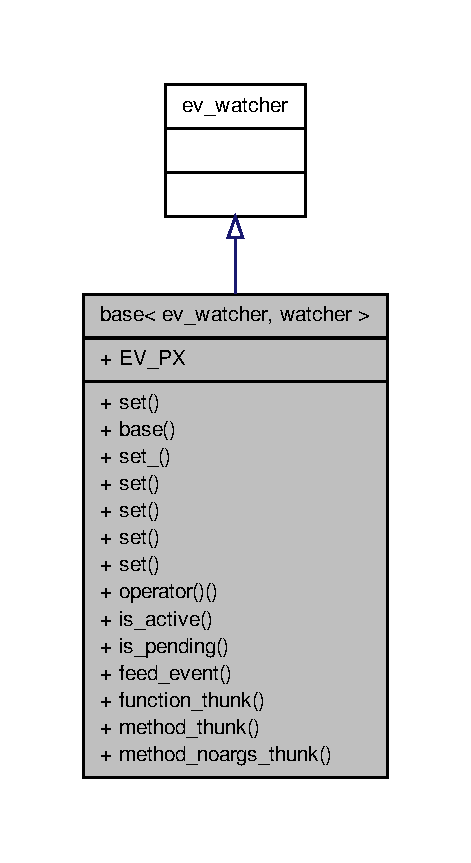
\includegraphics[width=226pt]{structev_1_1base__inherit__graph}
\end{center}
\end{figure}


\-Collaboration diagram for base$<$ ev\-\_\-watcher, watcher $>$\-:
\nopagebreak
\begin{figure}[H]
\begin{center}
\leavevmode
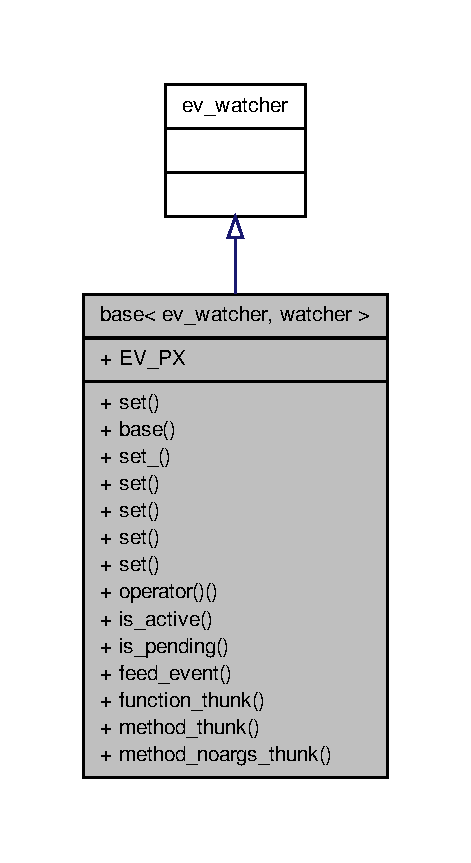
\includegraphics[width=226pt]{structev_1_1base__coll__graph}
\end{center}
\end{figure}
\subsection*{\-Public \-Member \-Functions}
\begin{DoxyCompactItemize}
\item 
void \hyperlink{structev_1_1base_ad02b7a6404f526c66ff2fba57579c9e5}{set} (\hyperlink{ev_8h_a6e6c6b499d18513c01cf4bde00121617}{\-E\-V\-\_\-\-P})  throw ()
\item 
\hyperlink{structev_1_1base_a773ad44efc538a04b3438ffad4a74bce}{base} (\hyperlink{structev_1_1base_a10f8def21e238e568c7bd2541aaae780}{\-E\-V\-\_\-\-P\-X})  throw ()
\item 
void \hyperlink{structev_1_1base_aec931fdffea513b4bff15b262dc0437d}{set\-\_\-} (const void $\ast$data, void($\ast$cb)(\hyperlink{ev_8h_a8ac42969e0a499b8c1367f0ad85dbba9}{\-E\-V\-\_\-\-P\-\_\-} \hyperlink{structev__watcher}{ev\-\_\-watcher} $\ast$w, int revents))  throw ()
\item 
{\footnotesize template$<$void($\ast$)(watcher \&w, int) function$>$ }\\void \hyperlink{structev_1_1base_affb794c41e2b56a976d5ecb7e78650a1}{set} (void $\ast$data=0)  throw ()
\item 
{\footnotesize template$<$class K , void(\-K\-::$\ast$)(watcher \&w, int) method$>$ }\\void \hyperlink{structev_1_1base_aad05c184ef537a75dc9f6863dc003dc7}{set} (\-K $\ast$object)  throw ()
\item 
{\footnotesize template$<$class K $>$ }\\void \hyperlink{structev_1_1base_a212d1dd3c68d3f8f3603b42e554db534}{set} (\-K $\ast$object)  throw ()
\item 
{\footnotesize template$<$class K , void(\-K\-::$\ast$)() method$>$ }\\void \hyperlink{structev_1_1base_aad05c184ef537a75dc9f6863dc003dc7}{set} (\-K $\ast$object)  throw ()
\item 
void \hyperlink{structev_1_1base_a698363269906e0658cab14ae31d959b5}{operator()} (int events=\hyperlink{ev_8h_abc6126af1d45847bc59afa0aa3216b04ad1171dcfff57cf1425e53bd38d69999d}{\-E\-V\-\_\-\-U\-N\-D\-E\-F})
\item 
bool \hyperlink{structev_1_1base_a1c6aa4f12f0decd6ae4e88b9ea361126}{is\-\_\-active} () const   throw ()
\item 
bool \hyperlink{structev_1_1base_a48b8b232d7917e357ffb0f1137ef9c38}{is\-\_\-pending} () const   throw ()
\item 
void \hyperlink{structev_1_1base_a19cf5d1f44332b12eaaf465b110b91b0}{feed\-\_\-event} (int revents)  throw ()
\end{DoxyCompactItemize}
\subsection*{\-Static \-Public \-Member \-Functions}
\begin{DoxyCompactItemize}
\item 
{\footnotesize template$<$void($\ast$)(watcher \&w, int) function$>$ }\\static void \hyperlink{structev_1_1base_ab6a9dbee5f754f64a234ad4e4d287d03}{function\-\_\-thunk} (\hyperlink{ev_8h_a8ac42969e0a499b8c1367f0ad85dbba9}{\-E\-V\-\_\-\-P\-\_\-} \hyperlink{structev__watcher}{ev\-\_\-watcher} $\ast$w, int revents)
\item 
{\footnotesize template$<$class K , void(\-K\-::$\ast$)(watcher \&w, int) method$>$ }\\static void \hyperlink{structev_1_1base_a8038092c2cdb65f0c09001e2eb846340}{method\-\_\-thunk} (\hyperlink{ev_8h_a8ac42969e0a499b8c1367f0ad85dbba9}{\-E\-V\-\_\-\-P\-\_\-} \hyperlink{structev__watcher}{ev\-\_\-watcher} $\ast$w, int revents)
\item 
{\footnotesize template$<$class K , void(\-K\-::$\ast$)() method$>$ }\\static void \hyperlink{structev_1_1base_a5baff17580ab861b158097ca00224adf}{method\-\_\-noargs\-\_\-thunk} (\hyperlink{ev_8h_a8ac42969e0a499b8c1367f0ad85dbba9}{\-E\-V\-\_\-\-P\-\_\-} \hyperlink{structev__watcher}{ev\-\_\-watcher} $\ast$w, int revents)
\end{DoxyCompactItemize}
\subsection*{\-Data \-Fields}
\begin{DoxyCompactItemize}
\item 
\hyperlink{structev_1_1base_a10f8def21e238e568c7bd2541aaae780}{\-E\-V\-\_\-\-P\-X}
\end{DoxyCompactItemize}


\subsection{\-Detailed \-Description}
\subsubsection*{template$<$class ev\-\_\-watcher, class watcher$>$struct ev\-::base$<$ ev\-\_\-watcher, watcher $>$}



\-Definition at line 422 of file ev++.\-h.



\subsection{\-Constructor \& \-Destructor \-Documentation}
\hypertarget{structev_1_1base_a773ad44efc538a04b3438ffad4a74bce}{\index{ev\-::base@{ev\-::base}!base@{base}}
\index{base@{base}!ev::base@{ev\-::base}}
\subsubsection[{base}]{\setlength{\rightskip}{0pt plus 5cm}{\bf base} (
\begin{DoxyParamCaption}
\item[{{\bf \-E\-V\-\_\-\-P\-X}}]{}
\end{DoxyParamCaption}
)  throw ()\hspace{0.3cm}{\ttfamily  \mbox{[}inline\mbox{]}}}}\label{structev_1_1base_a773ad44efc538a04b3438ffad4a74bce}


\-Definition at line 434 of file ev++.\-h.



\subsection{\-Member \-Function \-Documentation}
\hypertarget{structev_1_1base_a19cf5d1f44332b12eaaf465b110b91b0}{\index{ev\-::base@{ev\-::base}!feed\-\_\-event@{feed\-\_\-event}}
\index{feed\-\_\-event@{feed\-\_\-event}!ev::base@{ev\-::base}}
\subsubsection[{feed\-\_\-event}]{\setlength{\rightskip}{0pt plus 5cm}void {\bf feed\-\_\-event} (
\begin{DoxyParamCaption}
\item[{int}]{revents}
\end{DoxyParamCaption}
)  throw ()\hspace{0.3cm}{\ttfamily  \mbox{[}inline\mbox{]}}}}\label{structev_1_1base_a19cf5d1f44332b12eaaf465b110b91b0}


\-Definition at line 514 of file ev++.\-h.



\-Here is the call graph for this function\-:
\nopagebreak
\begin{figure}[H]
\begin{center}
\leavevmode
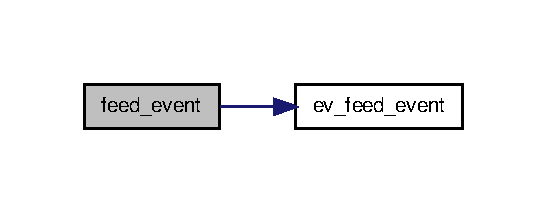
\includegraphics[width=262pt]{structev_1_1base_a19cf5d1f44332b12eaaf465b110b91b0_cgraph}
\end{center}
\end{figure}


\hypertarget{structev_1_1base_ab6a9dbee5f754f64a234ad4e4d287d03}{\index{ev\-::base@{ev\-::base}!function\-\_\-thunk@{function\-\_\-thunk}}
\index{function\-\_\-thunk@{function\-\_\-thunk}!ev::base@{ev\-::base}}
\subsubsection[{function\-\_\-thunk}]{\setlength{\rightskip}{0pt plus 5cm}static void {\bf function\-\_\-thunk} (
\begin{DoxyParamCaption}
\item[{{\bf \-E\-V\-\_\-\-P\-\_\-} {\bf ev\-\_\-watcher} $\ast$}]{w, }
\item[{int}]{revents}
\end{DoxyParamCaption}
)\hspace{0.3cm}{\ttfamily  \mbox{[}inline, static\mbox{]}}}}\label{structev_1_1base_ab6a9dbee5f754f64a234ad4e4d287d03}


\-Definition at line 456 of file ev++.\-h.

\hypertarget{structev_1_1base_a1c6aa4f12f0decd6ae4e88b9ea361126}{\index{ev\-::base@{ev\-::base}!is\-\_\-active@{is\-\_\-active}}
\index{is\-\_\-active@{is\-\_\-active}!ev::base@{ev\-::base}}
\subsubsection[{is\-\_\-active}]{\setlength{\rightskip}{0pt plus 5cm}bool {\bf is\-\_\-active} (
\begin{DoxyParamCaption}
{}
\end{DoxyParamCaption}
) const  throw ()\hspace{0.3cm}{\ttfamily  \mbox{[}inline\mbox{]}}}}\label{structev_1_1base_a1c6aa4f12f0decd6ae4e88b9ea361126}


\-Definition at line 504 of file ev++.\-h.

\hypertarget{structev_1_1base_a48b8b232d7917e357ffb0f1137ef9c38}{\index{ev\-::base@{ev\-::base}!is\-\_\-pending@{is\-\_\-pending}}
\index{is\-\_\-pending@{is\-\_\-pending}!ev::base@{ev\-::base}}
\subsubsection[{is\-\_\-pending}]{\setlength{\rightskip}{0pt plus 5cm}bool {\bf is\-\_\-pending} (
\begin{DoxyParamCaption}
{}
\end{DoxyParamCaption}
) const  throw ()\hspace{0.3cm}{\ttfamily  \mbox{[}inline\mbox{]}}}}\label{structev_1_1base_a48b8b232d7917e357ffb0f1137ef9c38}


\-Definition at line 509 of file ev++.\-h.

\hypertarget{structev_1_1base_a5baff17580ab861b158097ca00224adf}{\index{ev\-::base@{ev\-::base}!method\-\_\-noargs\-\_\-thunk@{method\-\_\-noargs\-\_\-thunk}}
\index{method\-\_\-noargs\-\_\-thunk@{method\-\_\-noargs\-\_\-thunk}!ev::base@{ev\-::base}}
\subsubsection[{method\-\_\-noargs\-\_\-thunk}]{\setlength{\rightskip}{0pt plus 5cm}static void {\bf method\-\_\-noargs\-\_\-thunk} (
\begin{DoxyParamCaption}
\item[{{\bf \-E\-V\-\_\-\-P\-\_\-} {\bf ev\-\_\-watcher} $\ast$}]{w, }
\item[{int}]{revents}
\end{DoxyParamCaption}
)\hspace{0.3cm}{\ttfamily  \mbox{[}inline, static\mbox{]}}}}\label{structev_1_1base_a5baff17580ab861b158097ca00224adf}


\-Definition at line 491 of file ev++.\-h.

\hypertarget{structev_1_1base_a8038092c2cdb65f0c09001e2eb846340}{\index{ev\-::base@{ev\-::base}!method\-\_\-thunk@{method\-\_\-thunk}}
\index{method\-\_\-thunk@{method\-\_\-thunk}!ev::base@{ev\-::base}}
\subsubsection[{method\-\_\-thunk}]{\setlength{\rightskip}{0pt plus 5cm}static void {\bf method\-\_\-thunk} (
\begin{DoxyParamCaption}
\item[{{\bf \-E\-V\-\_\-\-P\-\_\-} {\bf ev\-\_\-watcher} $\ast$}]{w, }
\item[{int}]{revents}
\end{DoxyParamCaption}
)\hspace{0.3cm}{\ttfamily  \mbox{[}inline, static\mbox{]}}}}\label{structev_1_1base_a8038092c2cdb65f0c09001e2eb846340}


\-Definition at line 477 of file ev++.\-h.



\-Here is the caller graph for this function\-:
\nopagebreak
\begin{figure}[H]
\begin{center}
\leavevmode
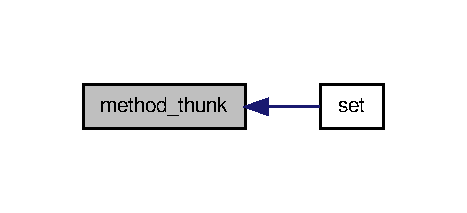
\includegraphics[width=224pt]{structev_1_1base_a8038092c2cdb65f0c09001e2eb846340_icgraph}
\end{center}
\end{figure}


\hypertarget{structev_1_1base_a698363269906e0658cab14ae31d959b5}{\index{ev\-::base@{ev\-::base}!operator()@{operator()}}
\index{operator()@{operator()}!ev::base@{ev\-::base}}
\subsubsection[{operator()}]{\setlength{\rightskip}{0pt plus 5cm}void operator() (
\begin{DoxyParamCaption}
\item[{int}]{events = {\ttfamily {\bf \-E\-V\-\_\-\-U\-N\-D\-E\-F}}}
\end{DoxyParamCaption}
)\hspace{0.3cm}{\ttfamily  \mbox{[}inline\mbox{]}}}}\label{structev_1_1base_a698363269906e0658cab14ae31d959b5}


\-Definition at line 497 of file ev++.\-h.

\hypertarget{structev_1_1base_ad02b7a6404f526c66ff2fba57579c9e5}{\index{ev\-::base@{ev\-::base}!set@{set}}
\index{set@{set}!ev::base@{ev\-::base}}
\subsubsection[{set}]{\setlength{\rightskip}{0pt plus 5cm}void {\bf set} (
\begin{DoxyParamCaption}
\item[{{\bf \-E\-V\-\_\-\-P}}]{}
\end{DoxyParamCaption}
)  throw ()\hspace{0.3cm}{\ttfamily  \mbox{[}inline\mbox{]}}}}\label{structev_1_1base_ad02b7a6404f526c66ff2fba57579c9e5}


\-Definition at line 428 of file ev++.\-h.

\hypertarget{structev_1_1base_affb794c41e2b56a976d5ecb7e78650a1}{\index{ev\-::base@{ev\-::base}!set@{set}}
\index{set@{set}!ev::base@{ev\-::base}}
\subsubsection[{set}]{\setlength{\rightskip}{0pt plus 5cm}void {\bf set} (
\begin{DoxyParamCaption}
\item[{void $\ast$}]{data = {\ttfamily 0}}
\end{DoxyParamCaption}
)  throw ()\hspace{0.3cm}{\ttfamily  \mbox{[}inline\mbox{]}}}}\label{structev_1_1base_affb794c41e2b56a976d5ecb7e78650a1}


\-Definition at line 450 of file ev++.\-h.



\-Here is the call graph for this function\-:
\nopagebreak
\begin{figure}[H]
\begin{center}
\leavevmode
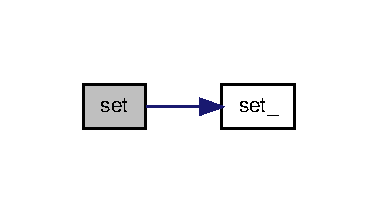
\includegraphics[width=182pt]{structev_1_1base_affb794c41e2b56a976d5ecb7e78650a1_cgraph}
\end{center}
\end{figure}


\hypertarget{structev_1_1base_aad05c184ef537a75dc9f6863dc003dc7}{\index{ev\-::base@{ev\-::base}!set@{set}}
\index{set@{set}!ev::base@{ev\-::base}}
\subsubsection[{set}]{\setlength{\rightskip}{0pt plus 5cm}void {\bf set} (
\begin{DoxyParamCaption}
\item[{\-K $\ast$}]{object}
\end{DoxyParamCaption}
)  throw ()\hspace{0.3cm}{\ttfamily  \mbox{[}inline\mbox{]}}}}\label{structev_1_1base_aad05c184ef537a75dc9f6863dc003dc7}


\-Definition at line 464 of file ev++.\-h.



\-Here is the call graph for this function\-:
\nopagebreak
\begin{figure}[H]
\begin{center}
\leavevmode
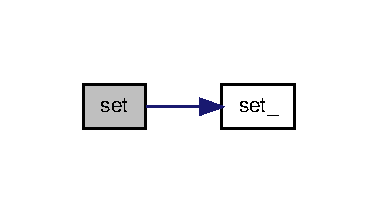
\includegraphics[width=182pt]{structev_1_1base_aad05c184ef537a75dc9f6863dc003dc7_cgraph}
\end{center}
\end{figure}


\hypertarget{structev_1_1base_a212d1dd3c68d3f8f3603b42e554db534}{\index{ev\-::base@{ev\-::base}!set@{set}}
\index{set@{set}!ev::base@{ev\-::base}}
\subsubsection[{set}]{\setlength{\rightskip}{0pt plus 5cm}void {\bf set} (
\begin{DoxyParamCaption}
\item[{\-K $\ast$}]{object}
\end{DoxyParamCaption}
)  throw ()\hspace{0.3cm}{\ttfamily  \mbox{[}inline\mbox{]}}}}\label{structev_1_1base_a212d1dd3c68d3f8f3603b42e554db534}


\-Definition at line 471 of file ev++.\-h.



\-Here is the call graph for this function\-:
\nopagebreak
\begin{figure}[H]
\begin{center}
\leavevmode
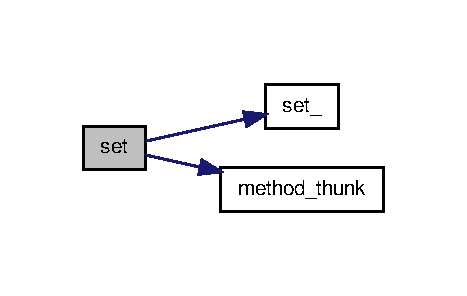
\includegraphics[width=224pt]{structev_1_1base_a212d1dd3c68d3f8f3603b42e554db534_cgraph}
\end{center}
\end{figure}


\hypertarget{structev_1_1base_aad05c184ef537a75dc9f6863dc003dc7}{\index{ev\-::base@{ev\-::base}!set@{set}}
\index{set@{set}!ev::base@{ev\-::base}}
\subsubsection[{set}]{\setlength{\rightskip}{0pt plus 5cm}void {\bf set} (
\begin{DoxyParamCaption}
\item[{\-K $\ast$}]{object}
\end{DoxyParamCaption}
)  throw ()\hspace{0.3cm}{\ttfamily  \mbox{[}inline\mbox{]}}}}\label{structev_1_1base_aad05c184ef537a75dc9f6863dc003dc7}


\-Definition at line 485 of file ev++.\-h.



\-Here is the call graph for this function\-:
\nopagebreak
\begin{figure}[H]
\begin{center}
\leavevmode
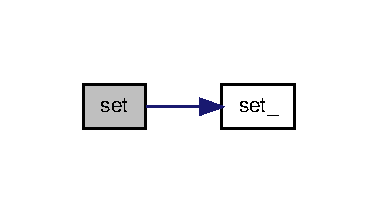
\includegraphics[width=182pt]{structev_1_1base_aad05c184ef537a75dc9f6863dc003dc7_cgraph}
\end{center}
\end{figure}


\hypertarget{structev_1_1base_aec931fdffea513b4bff15b262dc0437d}{\index{ev\-::base@{ev\-::base}!set\-\_\-@{set\-\_\-}}
\index{set\-\_\-@{set\-\_\-}!ev::base@{ev\-::base}}
\subsubsection[{set\-\_\-}]{\setlength{\rightskip}{0pt plus 5cm}void {\bf set\-\_\-} (
\begin{DoxyParamCaption}
\item[{const void $\ast$}]{data, }
\item[{void($\ast$)({\bf \-E\-V\-\_\-\-P\-\_\-} {\bf ev\-\_\-watcher} $\ast$w, int revents)}]{cb}
\end{DoxyParamCaption}
)  throw ()\hspace{0.3cm}{\ttfamily  \mbox{[}inline\mbox{]}}}}\label{structev_1_1base_aec931fdffea513b4bff15b262dc0437d}


\-Definition at line 442 of file ev++.\-h.



\-Here is the caller graph for this function\-:
\nopagebreak
\begin{figure}[H]
\begin{center}
\leavevmode
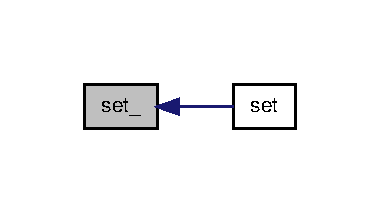
\includegraphics[width=182pt]{structev_1_1base_aec931fdffea513b4bff15b262dc0437d_icgraph}
\end{center}
\end{figure}




\subsection{\-Field \-Documentation}
\hypertarget{structev_1_1base_a10f8def21e238e568c7bd2541aaae780}{\index{ev\-::base@{ev\-::base}!\-E\-V\-\_\-\-P\-X@{\-E\-V\-\_\-\-P\-X}}
\index{\-E\-V\-\_\-\-P\-X@{\-E\-V\-\_\-\-P\-X}!ev::base@{ev\-::base}}
\subsubsection[{\-E\-V\-\_\-\-P\-X}]{\setlength{\rightskip}{0pt plus 5cm}{\bf \-E\-V\-\_\-\-P\-X}}}\label{structev_1_1base_a10f8def21e238e568c7bd2541aaae780}


\-Definition at line 425 of file ev++.\-h.



\-The documentation for this struct was generated from the following file\-:\begin{DoxyCompactItemize}
\item 
/home/jaymiao/workstation/github/libev-\/4.\-19/\hyperlink{ev_09_09_8h}{ev++.\-h}\end{DoxyCompactItemize}

\hypertarget{structev_1_1default__loop}{\section{default\-\_\-loop \-Struct \-Reference}
\label{structev_1_1default__loop}\index{default\-\_\-loop@{default\-\_\-loop}}
}


{\ttfamily \#include $<$ev++.\-h$>$}



\-Inheritance diagram for default\-\_\-loop\-:
\nopagebreak
\begin{figure}[H]
\begin{center}
\leavevmode
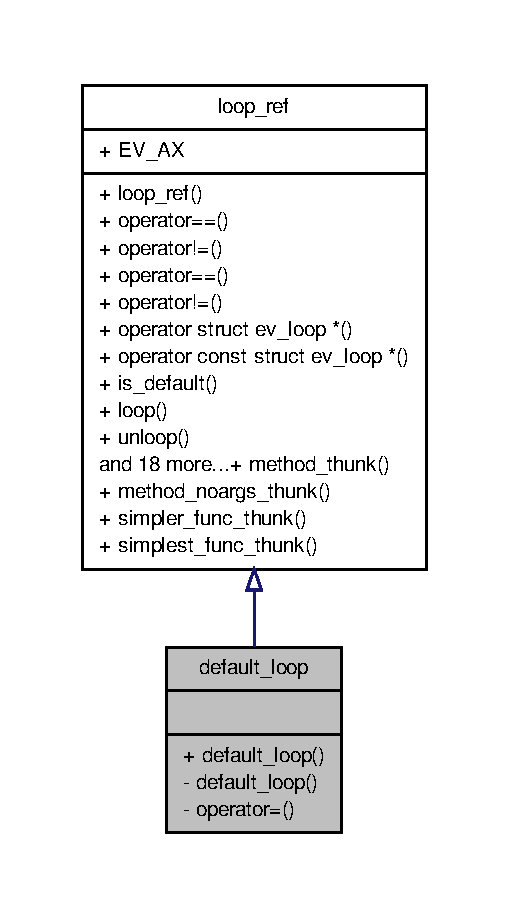
\includegraphics[width=244pt]{structev_1_1default__loop__inherit__graph}
\end{center}
\end{figure}


\-Collaboration diagram for default\-\_\-loop\-:
\nopagebreak
\begin{figure}[H]
\begin{center}
\leavevmode
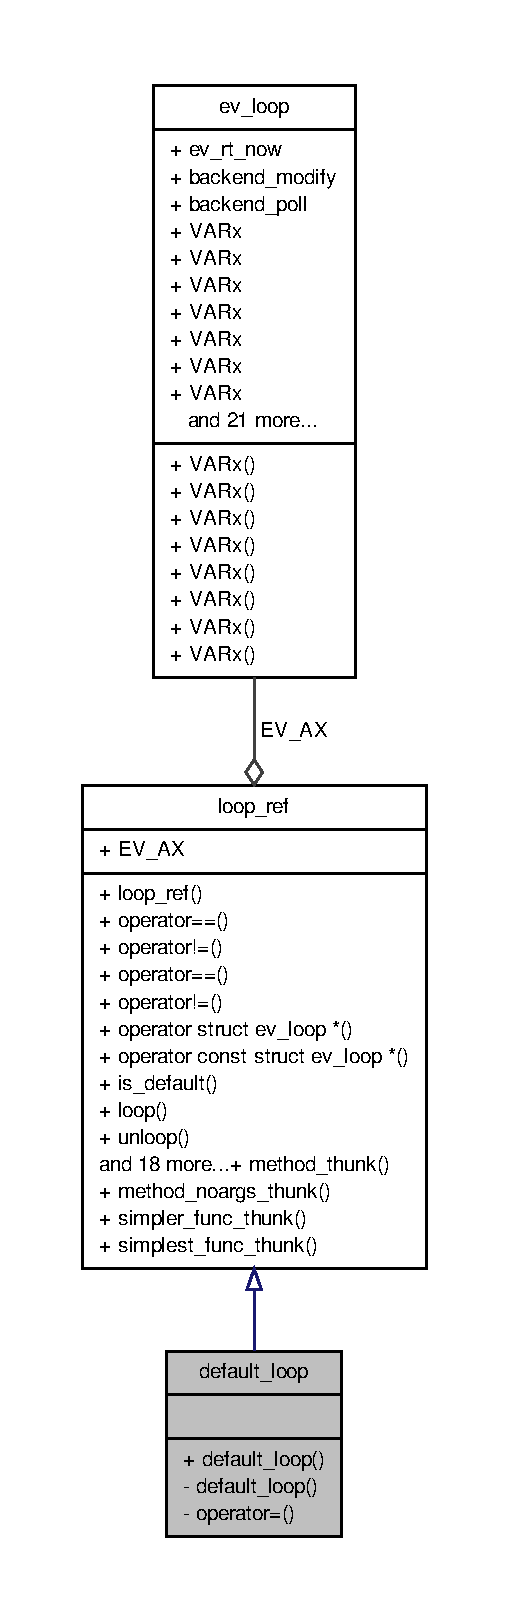
\includegraphics[height=550pt]{structev_1_1default__loop__coll__graph}
\end{center}
\end{figure}
\subsection*{\-Public \-Member \-Functions}
\begin{DoxyCompactItemize}
\item 
\hyperlink{structev_1_1default__loop_a3269f4b0cc758d91739d8184956b0461}{default\-\_\-loop} (unsigned int flags=\hyperlink{namespaceev_adf764cbdea00d65edcd07bb9953ad2b7aeef9468d1b98bca652a04bf5063fd9d6}{\-A\-U\-T\-O})  throw (bad\-\_\-loop)
\end{DoxyCompactItemize}
\subsection*{\-Private \-Member \-Functions}
\begin{DoxyCompactItemize}
\item 
\hyperlink{structev_1_1default__loop_ae4eb88a626b61e8515093279c9891157}{default\-\_\-loop} (const \hyperlink{structev_1_1default__loop}{default\-\_\-loop} \&)
\item 
\hyperlink{structev_1_1default__loop}{default\-\_\-loop} \& \hyperlink{structev_1_1default__loop_af74f9d916b4747983d5e13cd2e1d465d}{operator=} (const \hyperlink{structev_1_1default__loop}{default\-\_\-loop} \&)
\end{DoxyCompactItemize}


\subsection{\-Detailed \-Description}


\-Definition at line 377 of file ev++.\-h.



\subsection{\-Constructor \& \-Destructor \-Documentation}
\hypertarget{structev_1_1default__loop_a3269f4b0cc758d91739d8184956b0461}{\index{ev\-::default\-\_\-loop@{ev\-::default\-\_\-loop}!default\-\_\-loop@{default\-\_\-loop}}
\index{default\-\_\-loop@{default\-\_\-loop}!ev::default_loop@{ev\-::default\-\_\-loop}}
\subsubsection[{default\-\_\-loop}]{\setlength{\rightskip}{0pt plus 5cm}{\bf default\-\_\-loop} (
\begin{DoxyParamCaption}
\item[{unsigned int}]{flags = {\ttfamily {\bf \-A\-U\-T\-O}}}
\end{DoxyParamCaption}
)  throw ({\bf bad\-\_\-loop})\hspace{0.3cm}{\ttfamily  \mbox{[}inline\mbox{]}}}}\label{structev_1_1default__loop_a3269f4b0cc758d91739d8184956b0461}


\-Definition at line 379 of file ev++.\-h.



\-Here is the call graph for this function\-:
\nopagebreak
\begin{figure}[H]
\begin{center}
\leavevmode
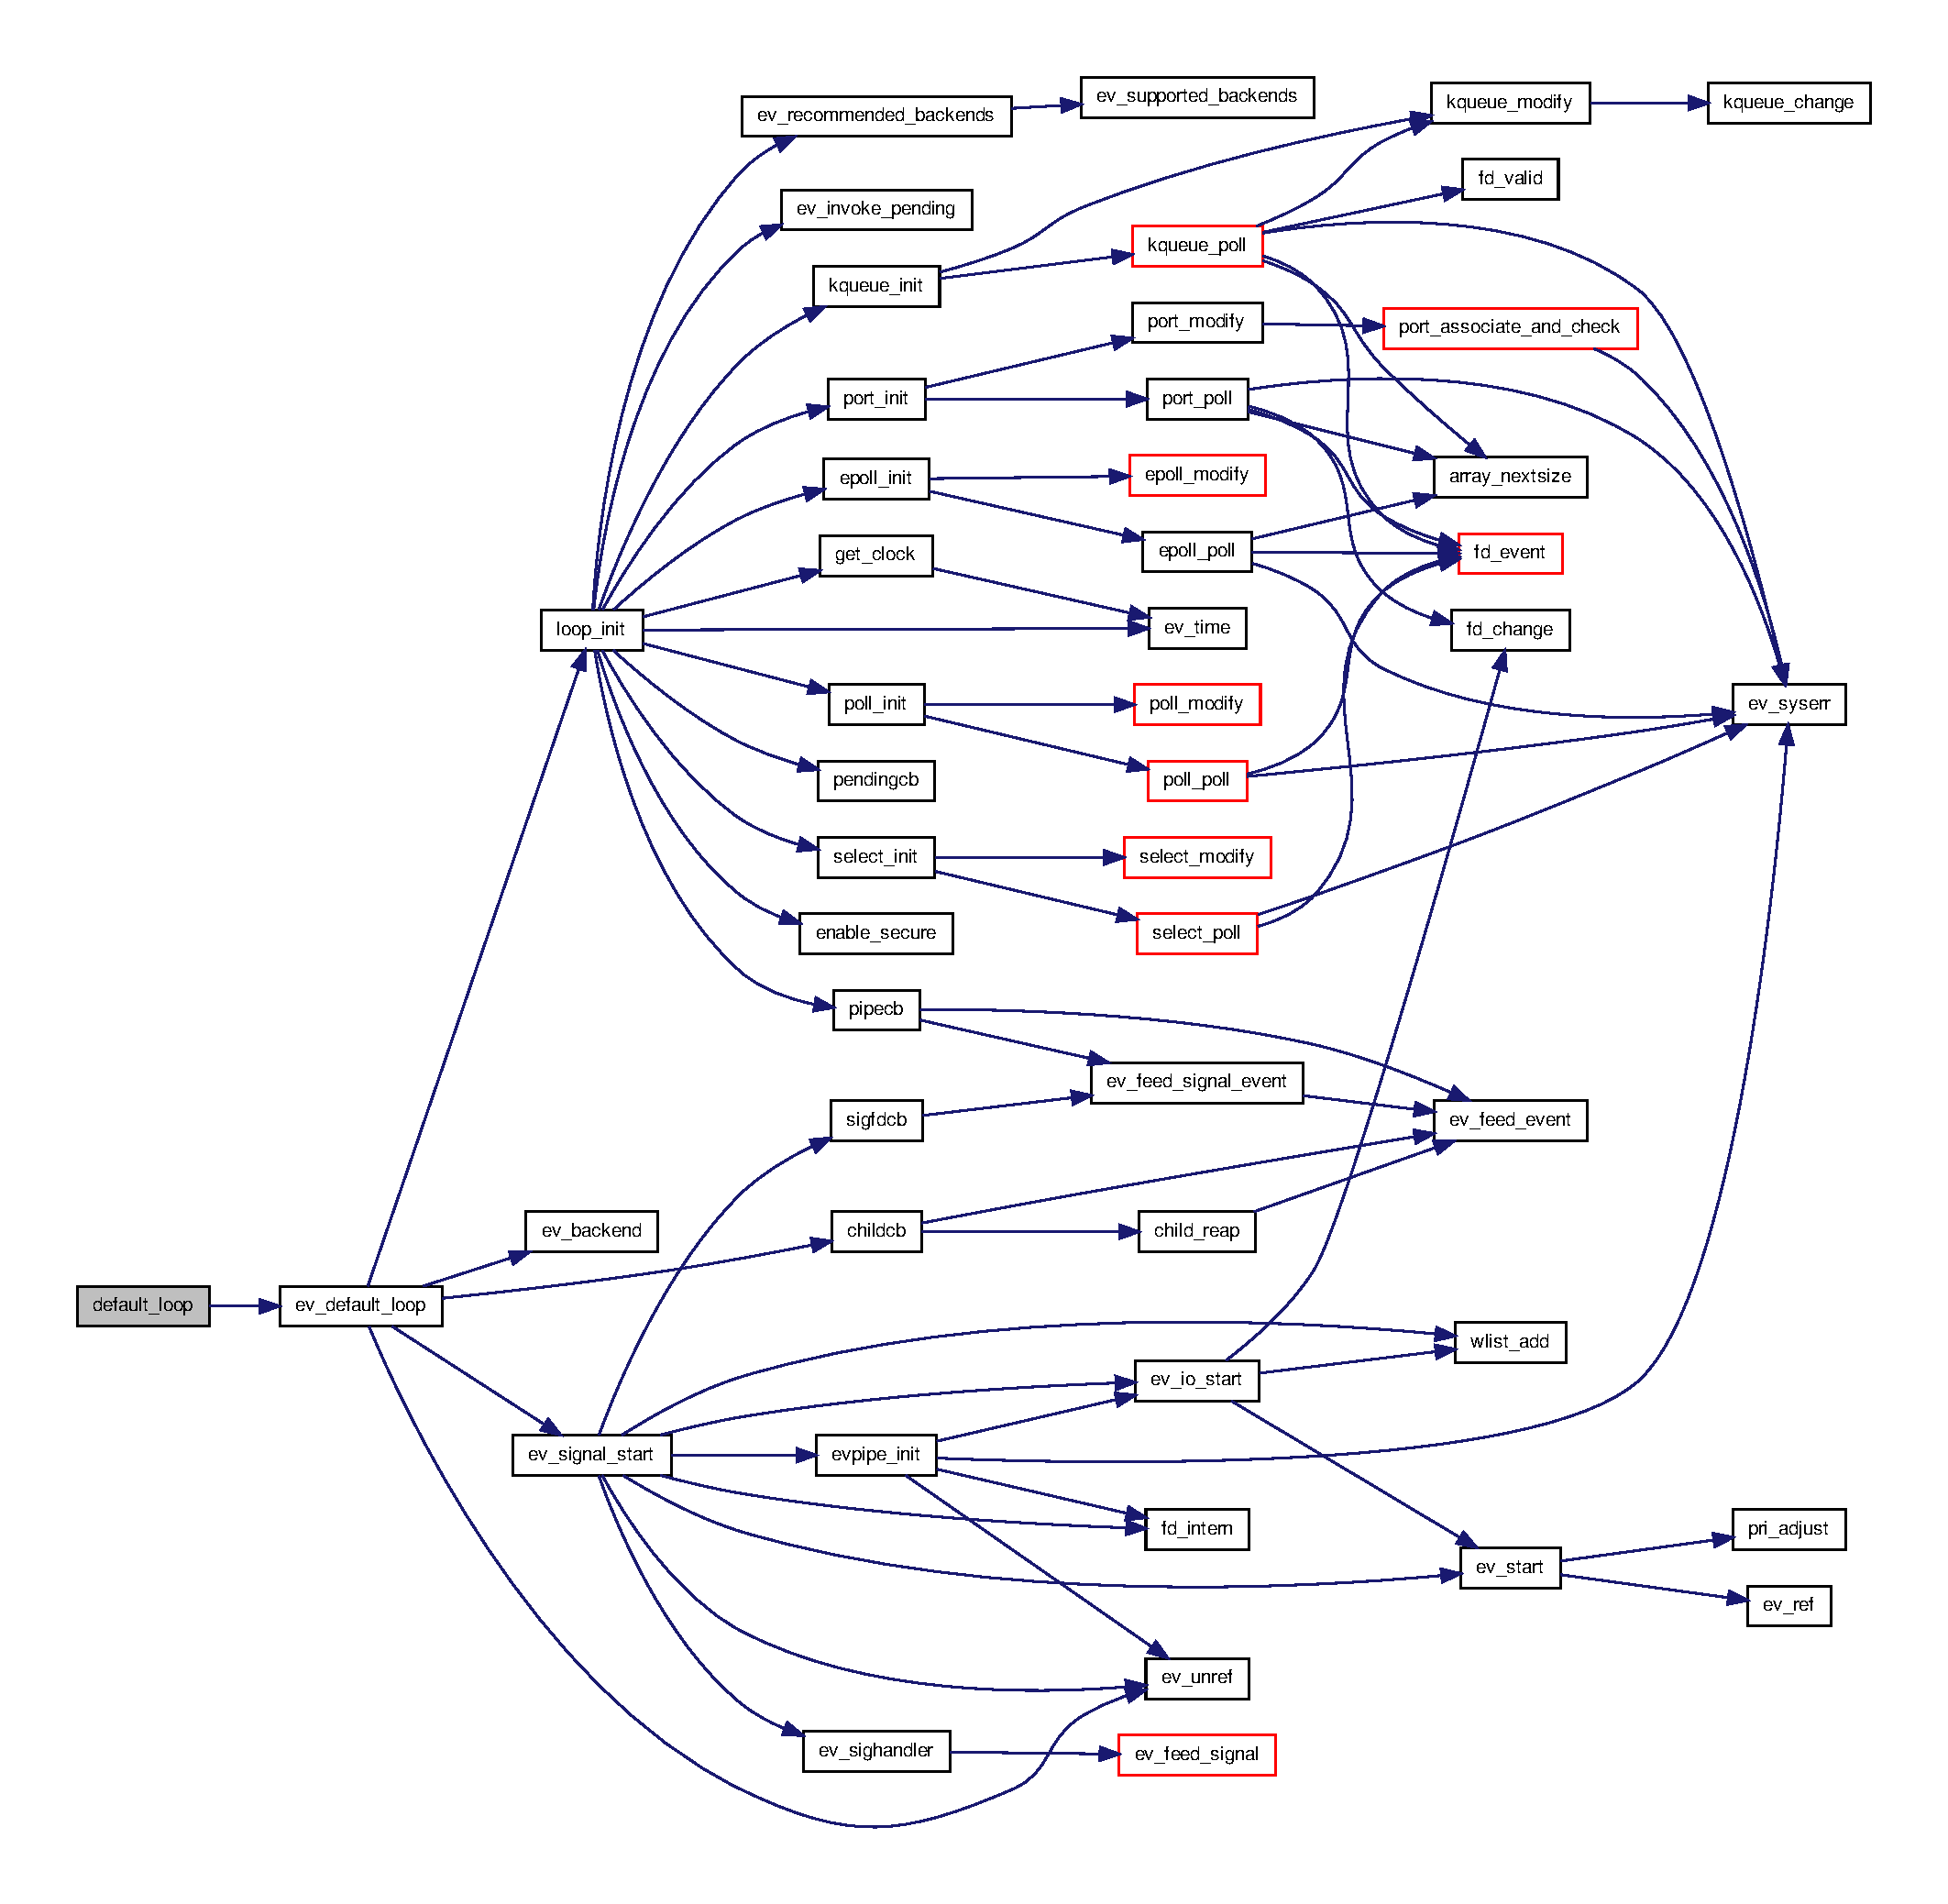
\includegraphics[width=350pt]{structev_1_1default__loop_a3269f4b0cc758d91739d8184956b0461_cgraph}
\end{center}
\end{figure}


\hypertarget{structev_1_1default__loop_ae4eb88a626b61e8515093279c9891157}{\index{ev\-::default\-\_\-loop@{ev\-::default\-\_\-loop}!default\-\_\-loop@{default\-\_\-loop}}
\index{default\-\_\-loop@{default\-\_\-loop}!ev::default_loop@{ev\-::default\-\_\-loop}}
\subsubsection[{default\-\_\-loop}]{\setlength{\rightskip}{0pt plus 5cm}{\bf default\-\_\-loop} (
\begin{DoxyParamCaption}
\item[{const {\bf default\-\_\-loop} \&}]{}
\end{DoxyParamCaption}
)\hspace{0.3cm}{\ttfamily  \mbox{[}private\mbox{]}}}}\label{structev_1_1default__loop_ae4eb88a626b61e8515093279c9891157}


\subsection{\-Member \-Function \-Documentation}
\hypertarget{structev_1_1default__loop_af74f9d916b4747983d5e13cd2e1d465d}{\index{ev\-::default\-\_\-loop@{ev\-::default\-\_\-loop}!operator=@{operator=}}
\index{operator=@{operator=}!ev::default_loop@{ev\-::default\-\_\-loop}}
\subsubsection[{operator=}]{\setlength{\rightskip}{0pt plus 5cm}{\bf default\-\_\-loop}\& operator= (
\begin{DoxyParamCaption}
\item[{const {\bf default\-\_\-loop} \&}]{}
\end{DoxyParamCaption}
)\hspace{0.3cm}{\ttfamily  \mbox{[}private\mbox{]}}}}\label{structev_1_1default__loop_af74f9d916b4747983d5e13cd2e1d465d}


\-The documentation for this struct was generated from the following file\-:\begin{DoxyCompactItemize}
\item 
/home/jaymiao/workstation/github/libev-\/4.\-19/\hyperlink{ev_09_09_8h}{ev++.\-h}\end{DoxyCompactItemize}

\hypertarget{structev_1_1dynamic__loop}{\section{dynamic\-\_\-loop \-Struct \-Reference}
\label{structev_1_1dynamic__loop}\index{dynamic\-\_\-loop@{dynamic\-\_\-loop}}
}


{\ttfamily \#include $<$ev++.\-h$>$}



\-Inheritance diagram for dynamic\-\_\-loop\-:
\nopagebreak
\begin{figure}[H]
\begin{center}
\leavevmode
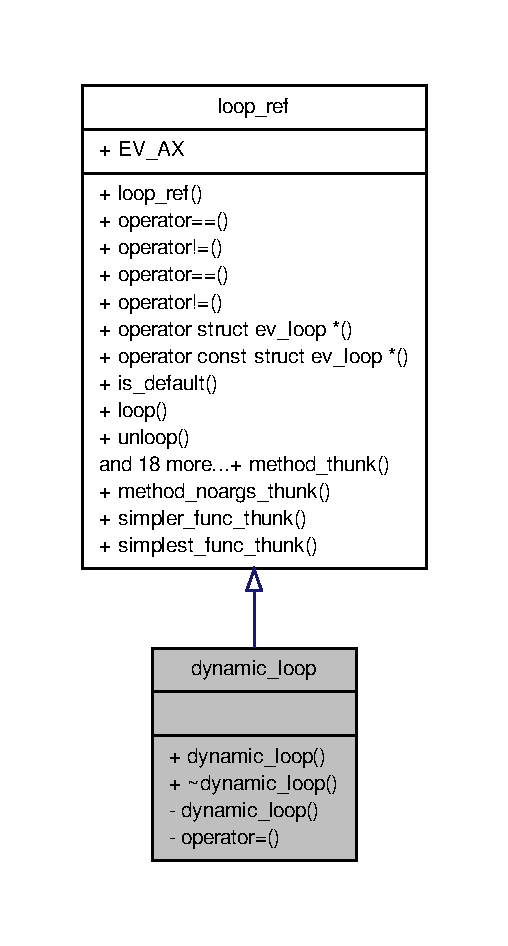
\includegraphics[width=244pt]{structev_1_1dynamic__loop__inherit__graph}
\end{center}
\end{figure}


\-Collaboration diagram for dynamic\-\_\-loop\-:
\nopagebreak
\begin{figure}[H]
\begin{center}
\leavevmode
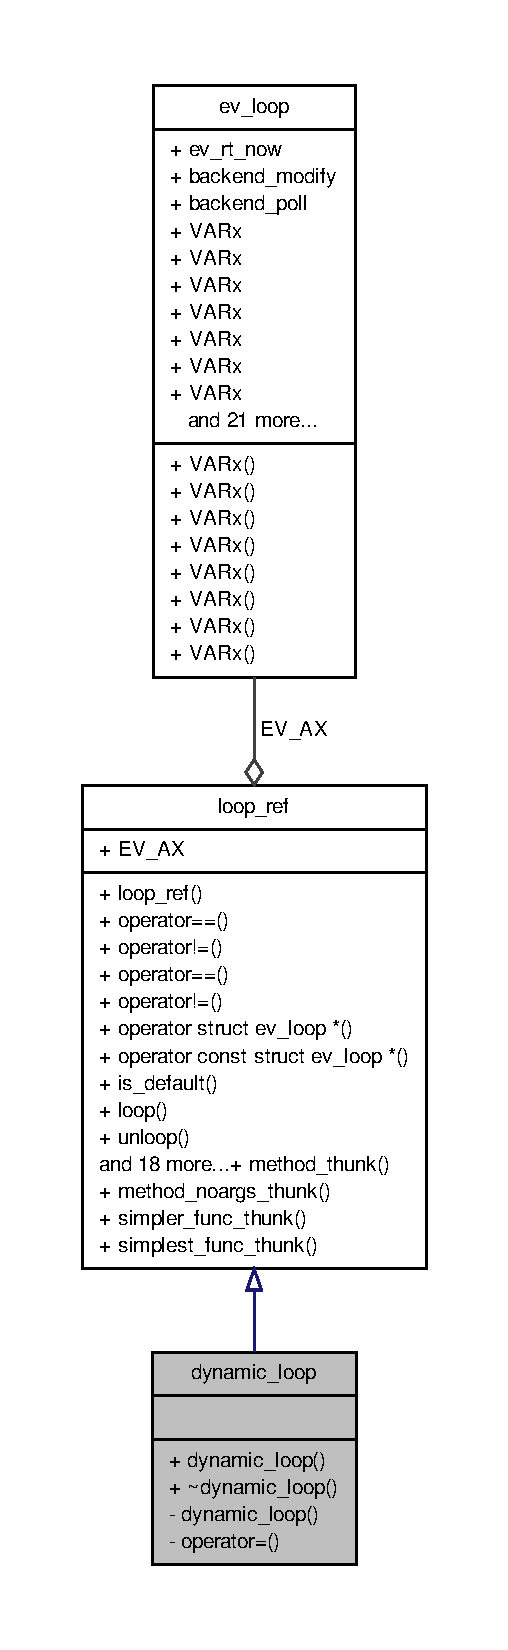
\includegraphics[height=550pt]{structev_1_1dynamic__loop__coll__graph}
\end{center}
\end{figure}
\subsection*{\-Public \-Member \-Functions}
\begin{DoxyCompactItemize}
\item 
\hyperlink{structev_1_1dynamic__loop_ab88a248ea377d7ab6a90a417eba8f3ed}{dynamic\-\_\-loop} (unsigned int flags=\hyperlink{namespaceev_adf764cbdea00d65edcd07bb9953ad2b7aeef9468d1b98bca652a04bf5063fd9d6}{\-A\-U\-T\-O})  throw (bad\-\_\-loop)
\item 
\hyperlink{structev_1_1dynamic__loop_a7fbbd0b59052f5afc3bb615dd5f8323d}{$\sim$dynamic\-\_\-loop} ()  throw ()
\end{DoxyCompactItemize}
\subsection*{\-Private \-Member \-Functions}
\begin{DoxyCompactItemize}
\item 
\hyperlink{structev_1_1dynamic__loop_aa12a9f226b5629df261ad670e877f117}{dynamic\-\_\-loop} (const \hyperlink{structev_1_1dynamic__loop}{dynamic\-\_\-loop} \&)
\item 
\hyperlink{structev_1_1dynamic__loop}{dynamic\-\_\-loop} \& \hyperlink{structev_1_1dynamic__loop_a2533758102f410ec6b7223cb72ae5dbc}{operator=} (const \hyperlink{structev_1_1dynamic__loop}{dynamic\-\_\-loop} \&)
\end{DoxyCompactItemize}


\subsection{\-Detailed \-Description}


\-Definition at line 352 of file ev++.\-h.



\subsection{\-Constructor \& \-Destructor \-Documentation}
\hypertarget{structev_1_1dynamic__loop_ab88a248ea377d7ab6a90a417eba8f3ed}{\index{ev\-::dynamic\-\_\-loop@{ev\-::dynamic\-\_\-loop}!dynamic\-\_\-loop@{dynamic\-\_\-loop}}
\index{dynamic\-\_\-loop@{dynamic\-\_\-loop}!ev::dynamic_loop@{ev\-::dynamic\-\_\-loop}}
\subsubsection[{dynamic\-\_\-loop}]{\setlength{\rightskip}{0pt plus 5cm}{\bf dynamic\-\_\-loop} (
\begin{DoxyParamCaption}
\item[{unsigned int}]{flags = {\ttfamily {\bf \-A\-U\-T\-O}}}
\end{DoxyParamCaption}
)  throw ({\bf bad\-\_\-loop})\hspace{0.3cm}{\ttfamily  \mbox{[}inline\mbox{]}}}}\label{structev_1_1dynamic__loop_ab88a248ea377d7ab6a90a417eba8f3ed}


\-Definition at line 355 of file ev++.\-h.

\hypertarget{structev_1_1dynamic__loop_a7fbbd0b59052f5afc3bb615dd5f8323d}{\index{ev\-::dynamic\-\_\-loop@{ev\-::dynamic\-\_\-loop}!$\sim$dynamic\-\_\-loop@{$\sim$dynamic\-\_\-loop}}
\index{$\sim$dynamic\-\_\-loop@{$\sim$dynamic\-\_\-loop}!ev::dynamic_loop@{ev\-::dynamic\-\_\-loop}}
\subsubsection[{$\sim$dynamic\-\_\-loop}]{\setlength{\rightskip}{0pt plus 5cm}$\sim${\bf dynamic\-\_\-loop} (
\begin{DoxyParamCaption}
{}
\end{DoxyParamCaption}
)  throw ()\hspace{0.3cm}{\ttfamily  \mbox{[}inline\mbox{]}}}}\label{structev_1_1dynamic__loop_a7fbbd0b59052f5afc3bb615dd5f8323d}


\-Definition at line 362 of file ev++.\-h.



\-Here is the call graph for this function\-:
\nopagebreak
\begin{figure}[H]
\begin{center}
\leavevmode
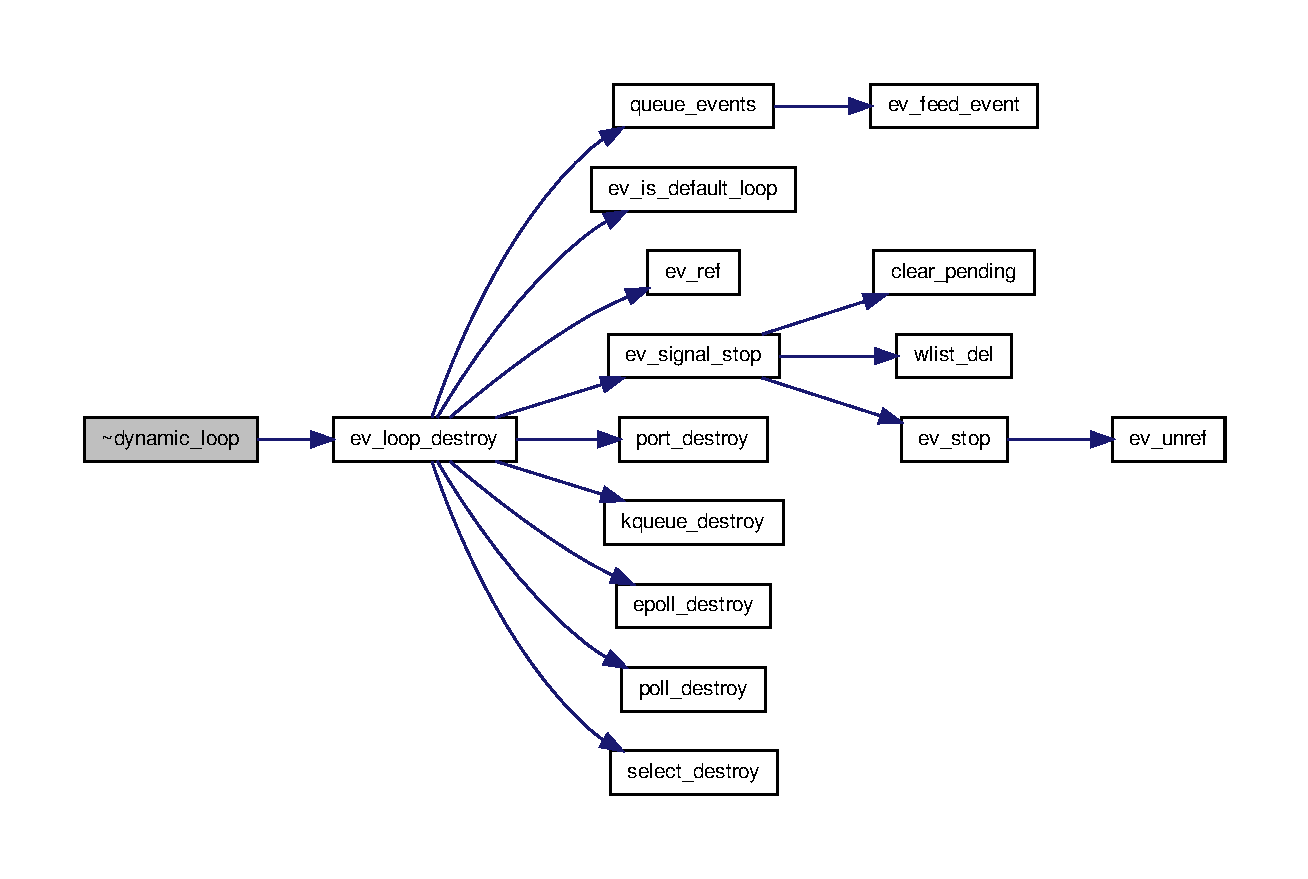
\includegraphics[width=350pt]{structev_1_1dynamic__loop_a7fbbd0b59052f5afc3bb615dd5f8323d_cgraph}
\end{center}
\end{figure}


\hypertarget{structev_1_1dynamic__loop_aa12a9f226b5629df261ad670e877f117}{\index{ev\-::dynamic\-\_\-loop@{ev\-::dynamic\-\_\-loop}!dynamic\-\_\-loop@{dynamic\-\_\-loop}}
\index{dynamic\-\_\-loop@{dynamic\-\_\-loop}!ev::dynamic_loop@{ev\-::dynamic\-\_\-loop}}
\subsubsection[{dynamic\-\_\-loop}]{\setlength{\rightskip}{0pt plus 5cm}{\bf dynamic\-\_\-loop} (
\begin{DoxyParamCaption}
\item[{const {\bf dynamic\-\_\-loop} \&}]{}
\end{DoxyParamCaption}
)\hspace{0.3cm}{\ttfamily  \mbox{[}private\mbox{]}}}}\label{structev_1_1dynamic__loop_aa12a9f226b5629df261ad670e877f117}


\subsection{\-Member \-Function \-Documentation}
\hypertarget{structev_1_1dynamic__loop_a2533758102f410ec6b7223cb72ae5dbc}{\index{ev\-::dynamic\-\_\-loop@{ev\-::dynamic\-\_\-loop}!operator=@{operator=}}
\index{operator=@{operator=}!ev::dynamic_loop@{ev\-::dynamic\-\_\-loop}}
\subsubsection[{operator=}]{\setlength{\rightskip}{0pt plus 5cm}{\bf dynamic\-\_\-loop}\& operator= (
\begin{DoxyParamCaption}
\item[{const {\bf dynamic\-\_\-loop} \&}]{}
\end{DoxyParamCaption}
)\hspace{0.3cm}{\ttfamily  \mbox{[}private\mbox{]}}}}\label{structev_1_1dynamic__loop_a2533758102f410ec6b7223cb72ae5dbc}


\-The documentation for this struct was generated from the following file\-:\begin{DoxyCompactItemize}
\item 
/home/jaymiao/workstation/github/libev-\/4.\-19/\hyperlink{ev_09_09_8h}{ev++.\-h}\end{DoxyCompactItemize}

\hypertarget{unionev__any__watcher}{\section{ev\-\_\-any\-\_\-watcher \-Union \-Reference}
\label{unionev__any__watcher}\index{ev\-\_\-any\-\_\-watcher@{ev\-\_\-any\-\_\-watcher}}
}


{\ttfamily \#include $<$ev.\-h$>$}



\-Collaboration diagram for ev\-\_\-any\-\_\-watcher\-:
\nopagebreak
\begin{figure}[H]
\begin{center}
\leavevmode
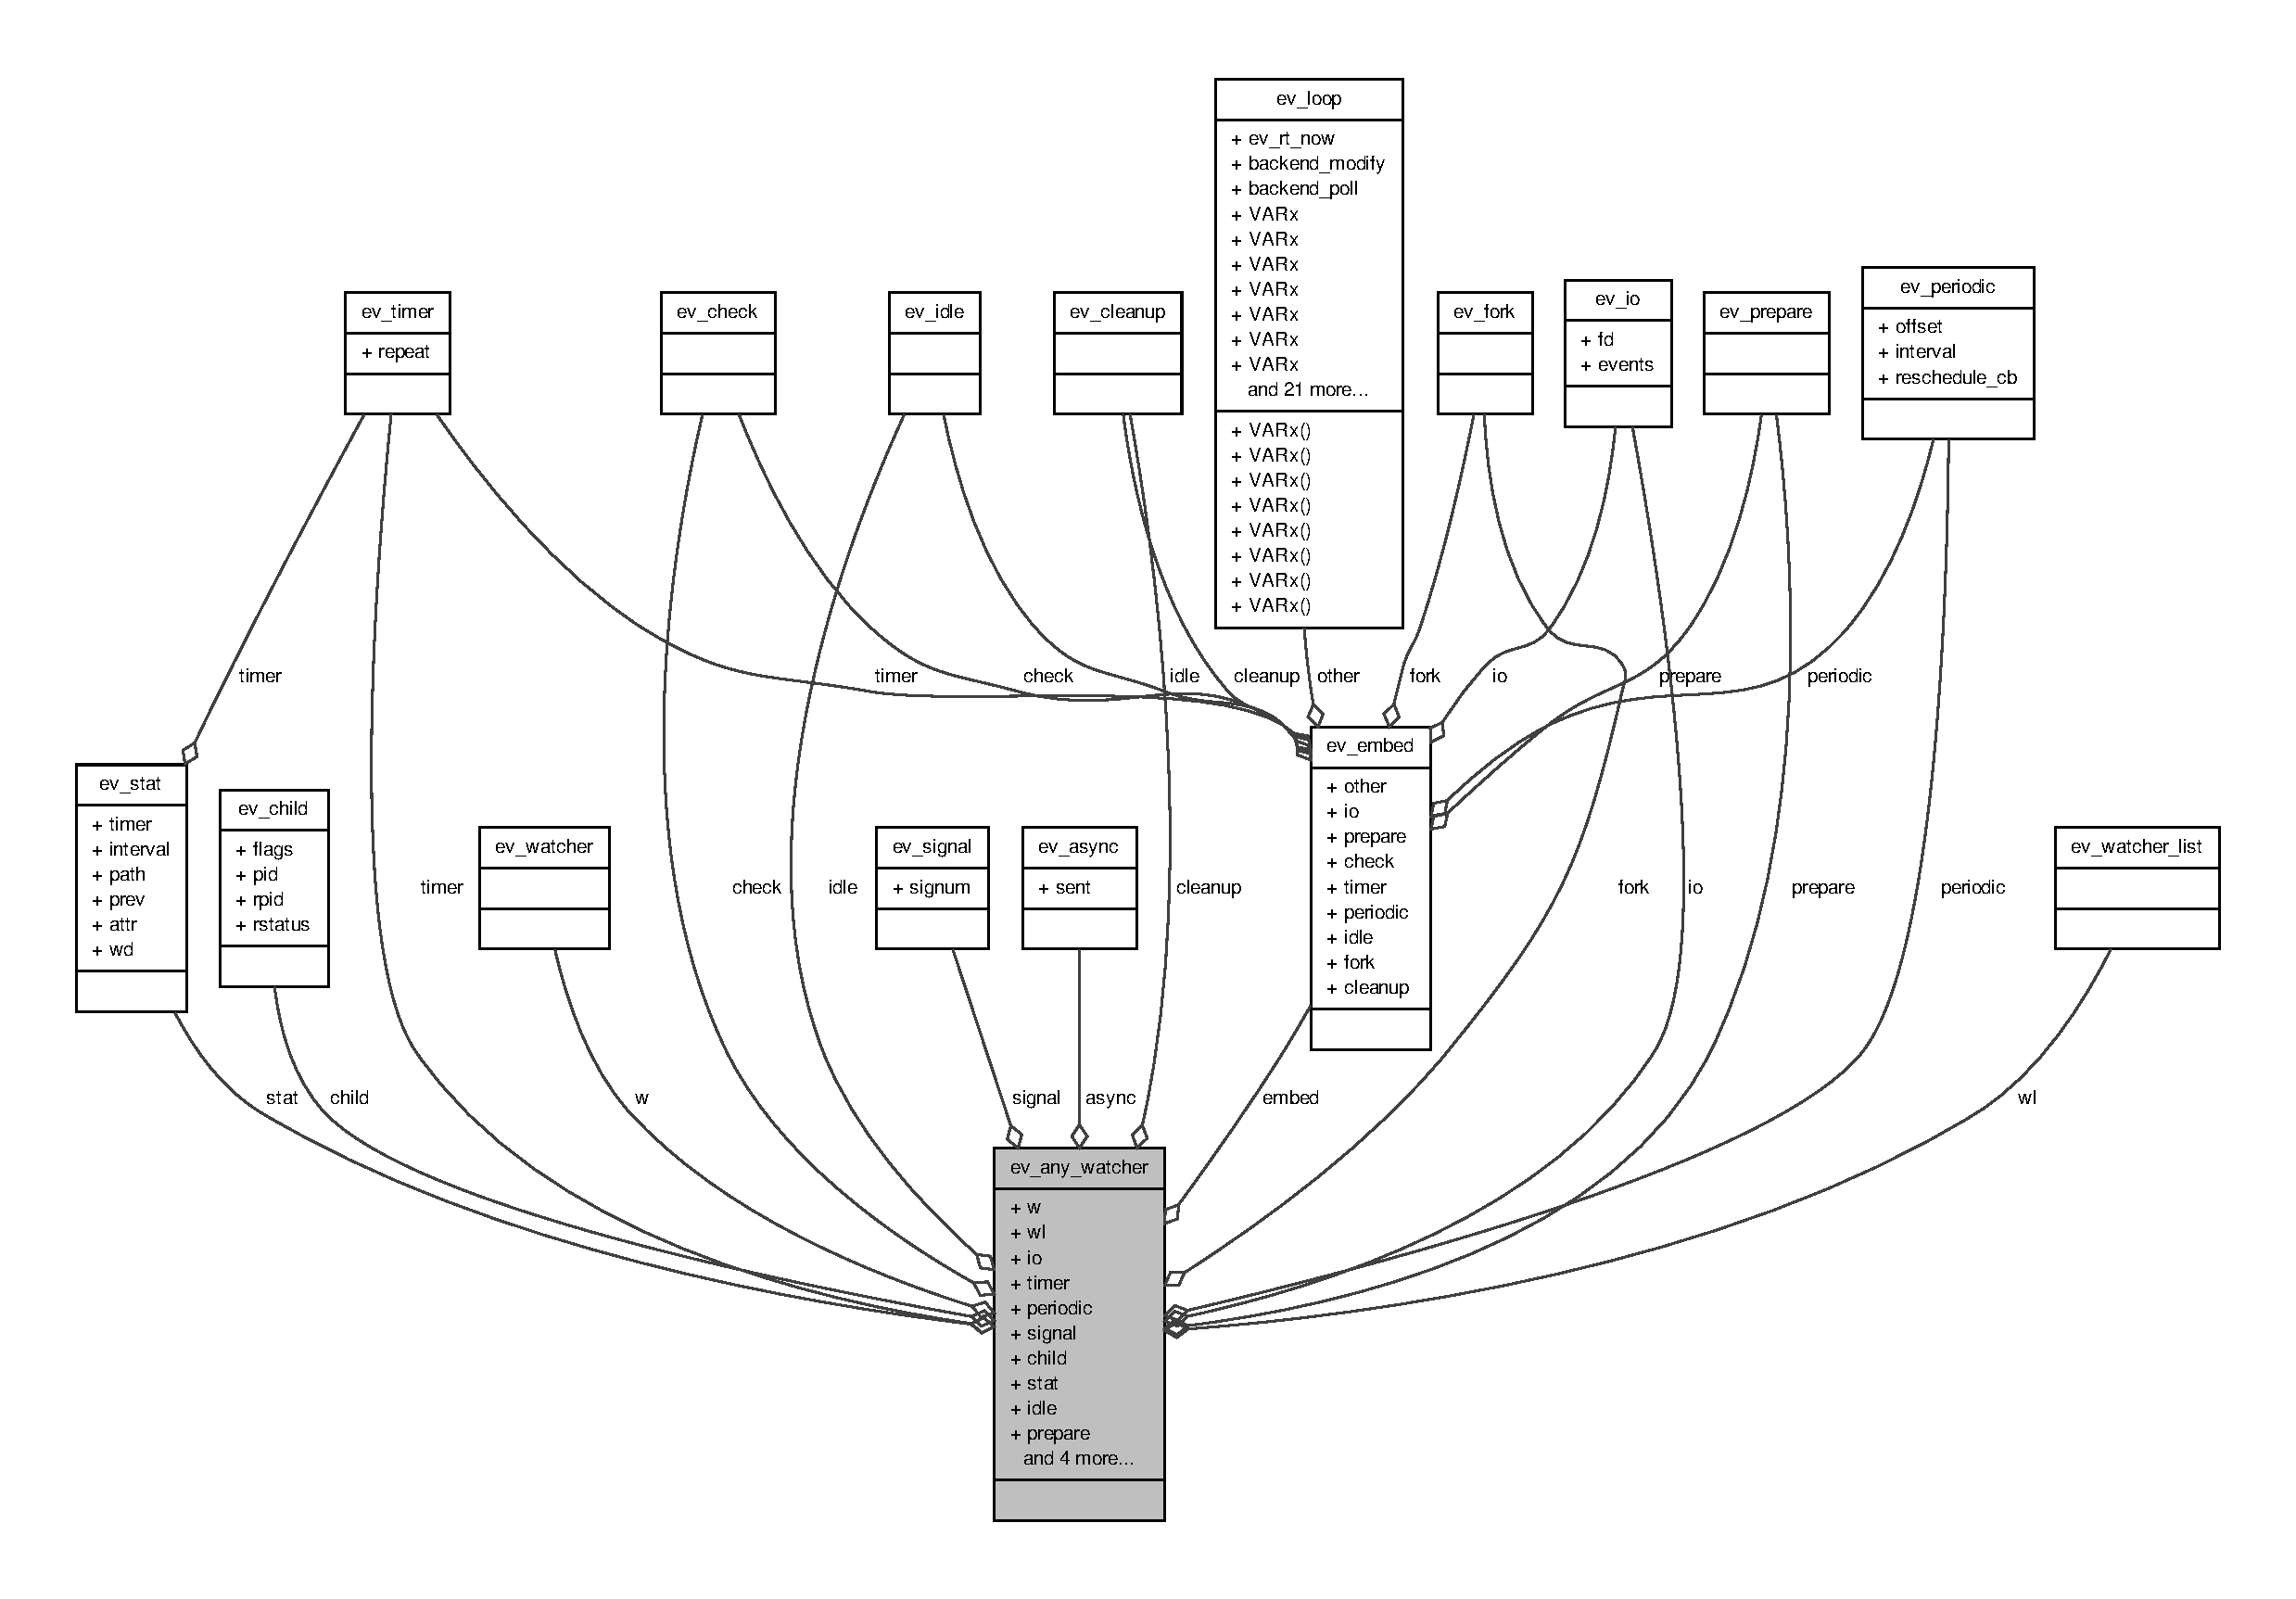
\includegraphics[width=350pt]{unionev__any__watcher__coll__graph}
\end{center}
\end{figure}
\subsection*{\-Data \-Fields}
\begin{DoxyCompactItemize}
\item 
struct \hyperlink{structev__watcher}{ev\-\_\-watcher} \hyperlink{unionev__any__watcher_a9516a8125893e72f22e7012717dad6d8}{w}
\item 
struct \hyperlink{structev__watcher__list}{ev\-\_\-watcher\-\_\-list} \hyperlink{unionev__any__watcher_ae2011b7703dba910528f85c51f9e2214}{wl}
\item 
struct \hyperlink{structev__io}{ev\-\_\-io} \hyperlink{unionev__any__watcher_a8a4fa321488e67a96ad783dc24187c4c}{io}
\item 
struct \hyperlink{structev__timer}{ev\-\_\-timer} \hyperlink{unionev__any__watcher_af2da8c0826c21eddd57a904ce5db7411}{timer}
\item 
struct \hyperlink{structev__periodic}{ev\-\_\-periodic} \hyperlink{unionev__any__watcher_a38b502fe39dbdf9208d295a9562781d0}{periodic}
\item 
struct \hyperlink{structev__signal}{ev\-\_\-signal} \hyperlink{unionev__any__watcher_a72308cea3a8da64c8b7e63a72645258b}{signal}
\item 
struct \hyperlink{structev__child}{ev\-\_\-child} \hyperlink{unionev__any__watcher_ae1125f192c1eb184294efd761ed9b7de}{child}
\item 
struct \hyperlink{structev__stat}{ev\-\_\-stat} \hyperlink{unionev__any__watcher_a4e2a569765766cdcda2cead6946aa7b5}{stat}
\item 
struct \hyperlink{structev__idle}{ev\-\_\-idle} \hyperlink{unionev__any__watcher_a873722b2eacfc6fdbf2cccbf3a3d90b9}{idle}
\item 
struct \hyperlink{structev__prepare}{ev\-\_\-prepare} \hyperlink{unionev__any__watcher_a87bf9c1da33923ce13a50b4fa6e2b572}{prepare}
\item 
struct \hyperlink{structev__check}{ev\-\_\-check} \hyperlink{unionev__any__watcher_a2b3de3d8f728c8ee5a2fc71499a6c4ea}{check}
\item 
struct \hyperlink{structev__fork}{ev\-\_\-fork} \hyperlink{unionev__any__watcher_ab915eaa6312f56672c8ca4cb1692e87c}{fork}
\item 
struct \hyperlink{structev__cleanup}{ev\-\_\-cleanup} \hyperlink{unionev__any__watcher_aeafce63f71f8dceb78babad901832f01}{cleanup}
\item 
struct \hyperlink{structev__embed}{ev\-\_\-embed} \hyperlink{unionev__any__watcher_abe8c0d216686c4c099394502acff8303}{embed}
\item 
struct \hyperlink{structev__async}{ev\-\_\-async} \hyperlink{unionev__any__watcher_a56b1e7af8c270020043037a796260aa1}{async}
\end{DoxyCompactItemize}


\subsection{\-Detailed \-Description}


\-Definition at line 462 of file ev.\-h.



\subsection{\-Field \-Documentation}
\hypertarget{unionev__any__watcher_a56b1e7af8c270020043037a796260aa1}{\index{ev\-\_\-any\-\_\-watcher@{ev\-\_\-any\-\_\-watcher}!async@{async}}
\index{async@{async}!ev_any_watcher@{ev\-\_\-any\-\_\-watcher}}
\subsubsection[{async}]{\setlength{\rightskip}{0pt plus 5cm}struct {\bf ev\-\_\-async} {\bf async}}}\label{unionev__any__watcher_a56b1e7af8c270020043037a796260aa1}


\-Definition at line 490 of file ev.\-h.

\hypertarget{unionev__any__watcher_a2b3de3d8f728c8ee5a2fc71499a6c4ea}{\index{ev\-\_\-any\-\_\-watcher@{ev\-\_\-any\-\_\-watcher}!check@{check}}
\index{check@{check}!ev_any_watcher@{ev\-\_\-any\-\_\-watcher}}
\subsubsection[{check}]{\setlength{\rightskip}{0pt plus 5cm}struct {\bf ev\-\_\-check} {\bf check}}}\label{unionev__any__watcher_a2b3de3d8f728c8ee5a2fc71499a6c4ea}


\-Definition at line 479 of file ev.\-h.

\hypertarget{unionev__any__watcher_ae1125f192c1eb184294efd761ed9b7de}{\index{ev\-\_\-any\-\_\-watcher@{ev\-\_\-any\-\_\-watcher}!child@{child}}
\index{child@{child}!ev_any_watcher@{ev\-\_\-any\-\_\-watcher}}
\subsubsection[{child}]{\setlength{\rightskip}{0pt plus 5cm}struct {\bf ev\-\_\-child} {\bf child}}}\label{unionev__any__watcher_ae1125f192c1eb184294efd761ed9b7de}


\-Definition at line 471 of file ev.\-h.

\hypertarget{unionev__any__watcher_aeafce63f71f8dceb78babad901832f01}{\index{ev\-\_\-any\-\_\-watcher@{ev\-\_\-any\-\_\-watcher}!cleanup@{cleanup}}
\index{cleanup@{cleanup}!ev_any_watcher@{ev\-\_\-any\-\_\-watcher}}
\subsubsection[{cleanup}]{\setlength{\rightskip}{0pt plus 5cm}struct {\bf ev\-\_\-cleanup} {\bf cleanup}}}\label{unionev__any__watcher_aeafce63f71f8dceb78babad901832f01}


\-Definition at line 484 of file ev.\-h.

\hypertarget{unionev__any__watcher_abe8c0d216686c4c099394502acff8303}{\index{ev\-\_\-any\-\_\-watcher@{ev\-\_\-any\-\_\-watcher}!embed@{embed}}
\index{embed@{embed}!ev_any_watcher@{ev\-\_\-any\-\_\-watcher}}
\subsubsection[{embed}]{\setlength{\rightskip}{0pt plus 5cm}struct {\bf ev\-\_\-embed} {\bf embed}}}\label{unionev__any__watcher_abe8c0d216686c4c099394502acff8303}


\-Definition at line 487 of file ev.\-h.

\hypertarget{unionev__any__watcher_ab915eaa6312f56672c8ca4cb1692e87c}{\index{ev\-\_\-any\-\_\-watcher@{ev\-\_\-any\-\_\-watcher}!fork@{fork}}
\index{fork@{fork}!ev_any_watcher@{ev\-\_\-any\-\_\-watcher}}
\subsubsection[{fork}]{\setlength{\rightskip}{0pt plus 5cm}struct {\bf ev\-\_\-fork} {\bf fork}}}\label{unionev__any__watcher_ab915eaa6312f56672c8ca4cb1692e87c}


\-Definition at line 481 of file ev.\-h.

\hypertarget{unionev__any__watcher_a873722b2eacfc6fdbf2cccbf3a3d90b9}{\index{ev\-\_\-any\-\_\-watcher@{ev\-\_\-any\-\_\-watcher}!idle@{idle}}
\index{idle@{idle}!ev_any_watcher@{ev\-\_\-any\-\_\-watcher}}
\subsubsection[{idle}]{\setlength{\rightskip}{0pt plus 5cm}struct {\bf ev\-\_\-idle} {\bf idle}}}\label{unionev__any__watcher_a873722b2eacfc6fdbf2cccbf3a3d90b9}


\-Definition at line 476 of file ev.\-h.

\hypertarget{unionev__any__watcher_a8a4fa321488e67a96ad783dc24187c4c}{\index{ev\-\_\-any\-\_\-watcher@{ev\-\_\-any\-\_\-watcher}!io@{io}}
\index{io@{io}!ev_any_watcher@{ev\-\_\-any\-\_\-watcher}}
\subsubsection[{io}]{\setlength{\rightskip}{0pt plus 5cm}struct {\bf ev\-\_\-io} {\bf io}}}\label{unionev__any__watcher_a8a4fa321488e67a96ad783dc24187c4c}


\-Definition at line 467 of file ev.\-h.

\hypertarget{unionev__any__watcher_a38b502fe39dbdf9208d295a9562781d0}{\index{ev\-\_\-any\-\_\-watcher@{ev\-\_\-any\-\_\-watcher}!periodic@{periodic}}
\index{periodic@{periodic}!ev_any_watcher@{ev\-\_\-any\-\_\-watcher}}
\subsubsection[{periodic}]{\setlength{\rightskip}{0pt plus 5cm}struct {\bf ev\-\_\-periodic} {\bf periodic}}}\label{unionev__any__watcher_a38b502fe39dbdf9208d295a9562781d0}


\-Definition at line 469 of file ev.\-h.

\hypertarget{unionev__any__watcher_a87bf9c1da33923ce13a50b4fa6e2b572}{\index{ev\-\_\-any\-\_\-watcher@{ev\-\_\-any\-\_\-watcher}!prepare@{prepare}}
\index{prepare@{prepare}!ev_any_watcher@{ev\-\_\-any\-\_\-watcher}}
\subsubsection[{prepare}]{\setlength{\rightskip}{0pt plus 5cm}struct {\bf ev\-\_\-prepare} {\bf prepare}}}\label{unionev__any__watcher_a87bf9c1da33923ce13a50b4fa6e2b572}


\-Definition at line 478 of file ev.\-h.

\hypertarget{unionev__any__watcher_a72308cea3a8da64c8b7e63a72645258b}{\index{ev\-\_\-any\-\_\-watcher@{ev\-\_\-any\-\_\-watcher}!signal@{signal}}
\index{signal@{signal}!ev_any_watcher@{ev\-\_\-any\-\_\-watcher}}
\subsubsection[{signal}]{\setlength{\rightskip}{0pt plus 5cm}struct {\bf ev\-\_\-signal} {\bf signal}}}\label{unionev__any__watcher_a72308cea3a8da64c8b7e63a72645258b}


\-Definition at line 470 of file ev.\-h.

\hypertarget{unionev__any__watcher_a4e2a569765766cdcda2cead6946aa7b5}{\index{ev\-\_\-any\-\_\-watcher@{ev\-\_\-any\-\_\-watcher}!stat@{stat}}
\index{stat@{stat}!ev_any_watcher@{ev\-\_\-any\-\_\-watcher}}
\subsubsection[{stat}]{\setlength{\rightskip}{0pt plus 5cm}struct {\bf ev\-\_\-stat} {\bf stat}}}\label{unionev__any__watcher_a4e2a569765766cdcda2cead6946aa7b5}


\-Definition at line 473 of file ev.\-h.

\hypertarget{unionev__any__watcher_af2da8c0826c21eddd57a904ce5db7411}{\index{ev\-\_\-any\-\_\-watcher@{ev\-\_\-any\-\_\-watcher}!timer@{timer}}
\index{timer@{timer}!ev_any_watcher@{ev\-\_\-any\-\_\-watcher}}
\subsubsection[{timer}]{\setlength{\rightskip}{0pt plus 5cm}struct {\bf ev\-\_\-timer} {\bf timer}}}\label{unionev__any__watcher_af2da8c0826c21eddd57a904ce5db7411}


\-Definition at line 468 of file ev.\-h.

\hypertarget{unionev__any__watcher_a9516a8125893e72f22e7012717dad6d8}{\index{ev\-\_\-any\-\_\-watcher@{ev\-\_\-any\-\_\-watcher}!w@{w}}
\index{w@{w}!ev_any_watcher@{ev\-\_\-any\-\_\-watcher}}
\subsubsection[{w}]{\setlength{\rightskip}{0pt plus 5cm}struct {\bf ev\-\_\-watcher} {\bf w}}}\label{unionev__any__watcher_a9516a8125893e72f22e7012717dad6d8}


\-Definition at line 464 of file ev.\-h.

\hypertarget{unionev__any__watcher_ae2011b7703dba910528f85c51f9e2214}{\index{ev\-\_\-any\-\_\-watcher@{ev\-\_\-any\-\_\-watcher}!wl@{wl}}
\index{wl@{wl}!ev_any_watcher@{ev\-\_\-any\-\_\-watcher}}
\subsubsection[{wl}]{\setlength{\rightskip}{0pt plus 5cm}struct {\bf ev\-\_\-watcher\-\_\-list} {\bf wl}}}\label{unionev__any__watcher_ae2011b7703dba910528f85c51f9e2214}


\-Definition at line 465 of file ev.\-h.



\-The documentation for this union was generated from the following file\-:\begin{DoxyCompactItemize}
\item 
/home/jaymiao/workstation/github/libev-\/4.\-19/\hyperlink{ev_8h}{ev.\-h}\end{DoxyCompactItemize}

\hypertarget{structev__async}{\section{ev\-\_\-async \-Struct \-Reference}
\label{structev__async}\index{ev\-\_\-async@{ev\-\_\-async}}
}


{\ttfamily \#include $<$ev.\-h$>$}

\subsection*{\-Data \-Fields}
\begin{DoxyCompactItemize}
\item 
\-E\-V\-\_\-\-A\-T\-O\-M\-I\-C\-\_\-\-T \hyperlink{structev__async_a52c67fd03d9b7f249d27026d864d6192}{sent}
\end{DoxyCompactItemize}


\subsection{\-Detailed \-Description}


\-Definition at line 451 of file ev.\-h.



\subsection{\-Field \-Documentation}
\hypertarget{structev__async_a52c67fd03d9b7f249d27026d864d6192}{\index{ev\-\_\-async@{ev\-\_\-async}!sent@{sent}}
\index{sent@{sent}!ev_async@{ev\-\_\-async}}
\subsubsection[{sent}]{\setlength{\rightskip}{0pt plus 5cm}\-E\-V\-\_\-\-A\-T\-O\-M\-I\-C\-\_\-\-T {\bf sent}}}\label{structev__async_a52c67fd03d9b7f249d27026d864d6192}


\-Definition at line 455 of file ev.\-h.



\-The documentation for this struct was generated from the following file\-:\begin{DoxyCompactItemize}
\item 
/home/jaymiao/workstation/github/libev-\/4.\-19/\hyperlink{ev_8h}{ev.\-h}\end{DoxyCompactItemize}

\hypertarget{structev__check}{\section{ev\-\_\-check \-Struct \-Reference}
\label{structev__check}\index{ev\-\_\-check@{ev\-\_\-check}}
}


{\ttfamily \#include $<$ev.\-h$>$}



\subsection{\-Detailed \-Description}


\-Definition at line 404 of file ev.\-h.



\-The documentation for this struct was generated from the following file\-:\begin{DoxyCompactItemize}
\item 
/home/jaymiao/workstation/github/libev-\/4.\-19/\hyperlink{ev_8h}{ev.\-h}\end{DoxyCompactItemize}

\hypertarget{structev__child}{\section{ev\-\_\-child \-Struct \-Reference}
\label{structev__child}\index{ev\-\_\-child@{ev\-\_\-child}}
}


{\ttfamily \#include $<$ev.\-h$>$}

\subsection*{\-Data \-Fields}
\begin{DoxyCompactItemize}
\item 
int \hyperlink{structev__child_ac8bf36fe0577cba66bccda3a6f7e80a4}{flags}
\item 
int \hyperlink{structev__child_af500917c052066b40cf47f96b43c607b}{pid}
\item 
int \hyperlink{structev__child_afab9955a3bac28037233de894654d9e7}{rpid}
\item 
int \hyperlink{structev__child_ac5fa58bd2072d4433fb143a734f54c1c}{rstatus}
\end{DoxyCompactItemize}


\subsection{\-Detailed \-Description}


\-Definition at line 351 of file ev.\-h.



\subsection{\-Field \-Documentation}
\hypertarget{structev__child_ac8bf36fe0577cba66bccda3a6f7e80a4}{\index{ev\-\_\-child@{ev\-\_\-child}!flags@{flags}}
\index{flags@{flags}!ev_child@{ev\-\_\-child}}
\subsubsection[{flags}]{\setlength{\rightskip}{0pt plus 5cm}int {\bf flags}}}\label{structev__child_ac8bf36fe0577cba66bccda3a6f7e80a4}


\-Definition at line 355 of file ev.\-h.

\hypertarget{structev__child_af500917c052066b40cf47f96b43c607b}{\index{ev\-\_\-child@{ev\-\_\-child}!pid@{pid}}
\index{pid@{pid}!ev_child@{ev\-\_\-child}}
\subsubsection[{pid}]{\setlength{\rightskip}{0pt plus 5cm}int {\bf pid}}}\label{structev__child_af500917c052066b40cf47f96b43c607b}


\-Definition at line 356 of file ev.\-h.

\hypertarget{structev__child_afab9955a3bac28037233de894654d9e7}{\index{ev\-\_\-child@{ev\-\_\-child}!rpid@{rpid}}
\index{rpid@{rpid}!ev_child@{ev\-\_\-child}}
\subsubsection[{rpid}]{\setlength{\rightskip}{0pt plus 5cm}int {\bf rpid}}}\label{structev__child_afab9955a3bac28037233de894654d9e7}


\-Definition at line 357 of file ev.\-h.

\hypertarget{structev__child_ac5fa58bd2072d4433fb143a734f54c1c}{\index{ev\-\_\-child@{ev\-\_\-child}!rstatus@{rstatus}}
\index{rstatus@{rstatus}!ev_child@{ev\-\_\-child}}
\subsubsection[{rstatus}]{\setlength{\rightskip}{0pt plus 5cm}int {\bf rstatus}}}\label{structev__child_ac5fa58bd2072d4433fb143a734f54c1c}


\-Definition at line 358 of file ev.\-h.



\-The documentation for this struct was generated from the following file\-:\begin{DoxyCompactItemize}
\item 
/home/jaymiao/workstation/github/libev-\/4.\-19/\hyperlink{ev_8h}{ev.\-h}\end{DoxyCompactItemize}

\hypertarget{structev__cleanup}{\section{ev\-\_\-cleanup \-Struct \-Reference}
\label{structev__cleanup}\index{ev\-\_\-cleanup@{ev\-\_\-cleanup}}
}


{\ttfamily \#include $<$ev.\-h$>$}



\subsection{\-Detailed \-Description}


\-Definition at line 421 of file ev.\-h.



\-The documentation for this struct was generated from the following file\-:\begin{DoxyCompactItemize}
\item 
/home/jaymiao/workstation/github/libev-\/4.\-19/\hyperlink{ev_8h}{ev.\-h}\end{DoxyCompactItemize}

\hypertarget{structev__embed}{\section{ev\-\_\-embed \-Struct \-Reference}
\label{structev__embed}\index{ev\-\_\-embed@{ev\-\_\-embed}}
}


{\ttfamily \#include $<$ev.\-h$>$}



\-Collaboration diagram for ev\-\_\-embed\-:
\nopagebreak
\begin{figure}[H]
\begin{center}
\leavevmode
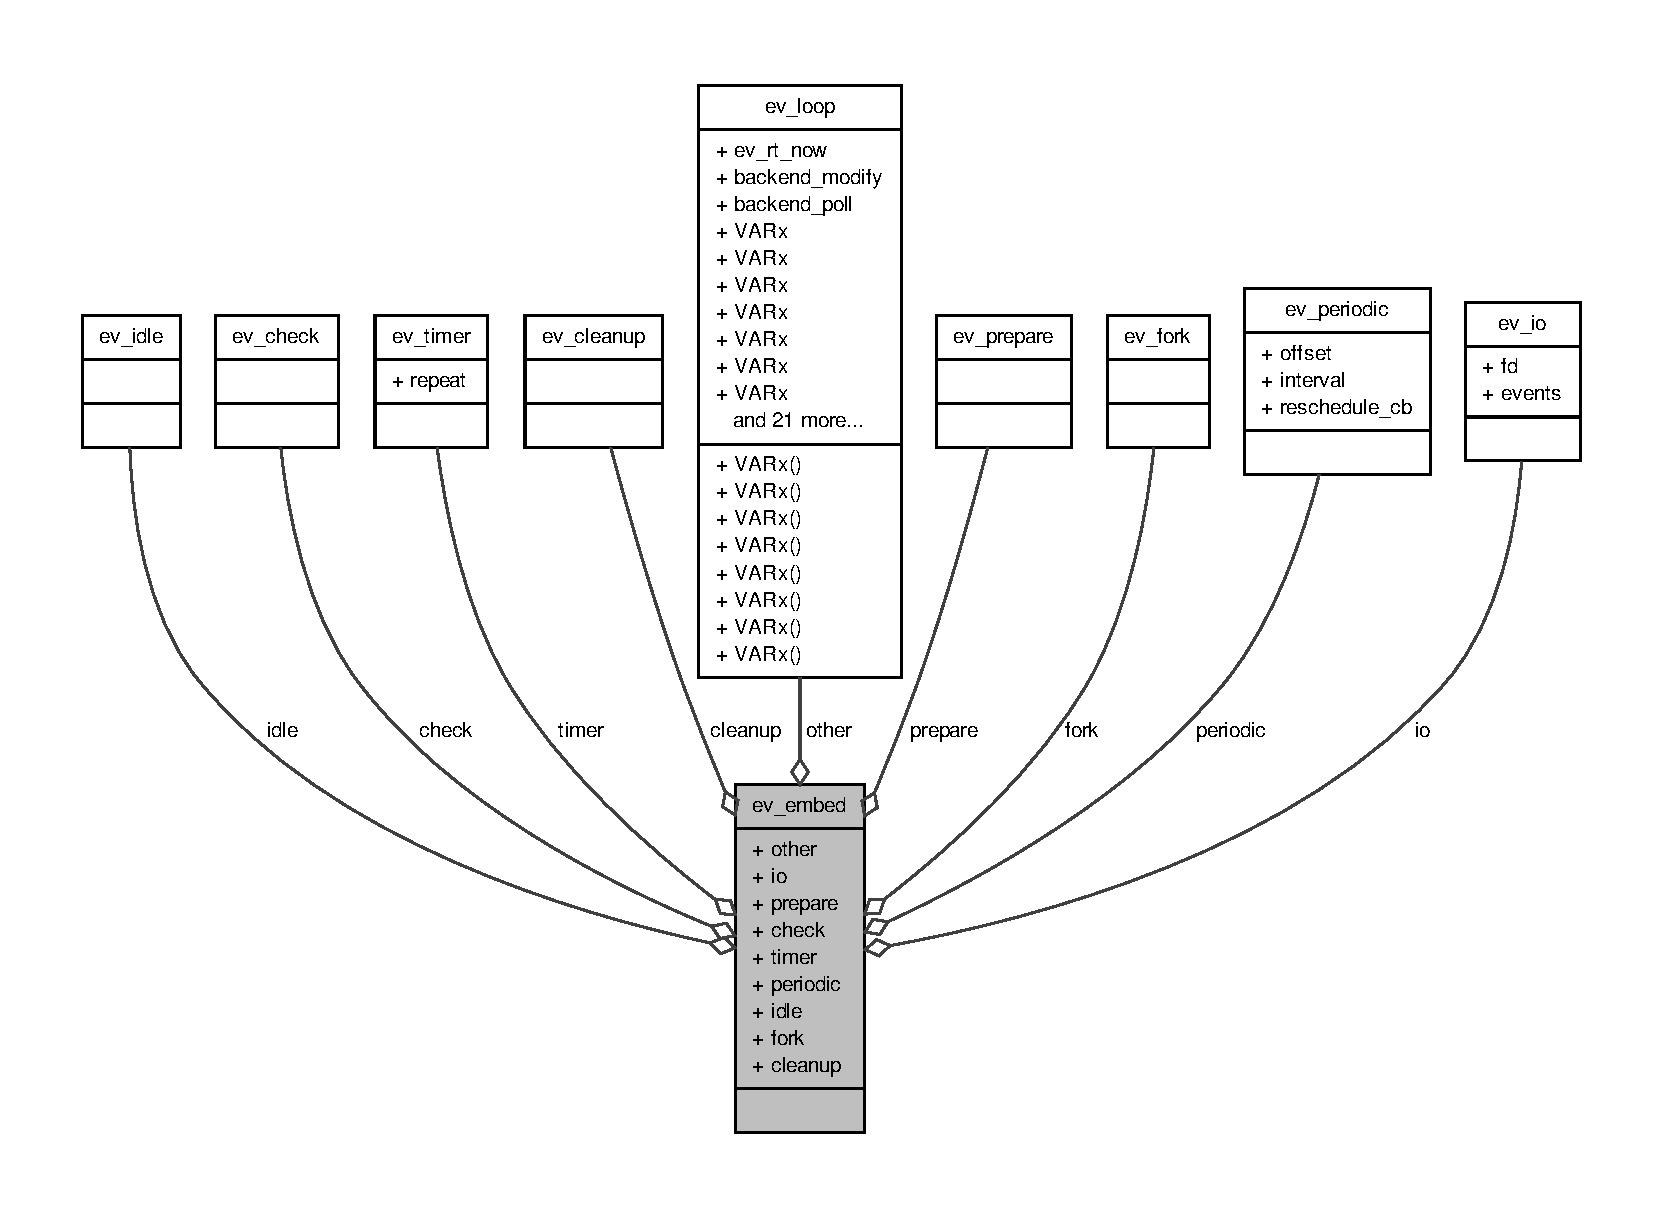
\includegraphics[width=350pt]{structev__embed__coll__graph}
\end{center}
\end{figure}
\subsection*{\-Data \-Fields}
\begin{DoxyCompactItemize}
\item 
struct \hyperlink{structev__loop}{ev\-\_\-loop} $\ast$ \hyperlink{structev__embed_a3079967d5620f0904f31db1f995d74e4}{other}
\item 
\hyperlink{structev__io}{ev\-\_\-io} \hyperlink{structev__embed_a0a60f96152fbb4f3d01c7ef3e4a3d856}{io}
\item 
\hyperlink{structev__prepare}{ev\-\_\-prepare} \hyperlink{structev__embed_a4e3f46ebebe0a3daf2a1f6b8ffef7cb8}{prepare}
\item 
\hyperlink{structev__check}{ev\-\_\-check} \hyperlink{structev__embed_a8e8591c0489d40ffb4c1a9060b39a7f4}{check}
\item 
\hyperlink{structev__timer}{ev\-\_\-timer} \hyperlink{structev__embed_a56d2f62405e7a2bba42204f714803c7c}{timer}
\item 
\hyperlink{structev__periodic}{ev\-\_\-periodic} \hyperlink{structev__embed_a5fbe01d0d9d8a54f2917d9d591496e4f}{periodic}
\item 
\hyperlink{structev__idle}{ev\-\_\-idle} \hyperlink{structev__embed_ae72313f3ce18355b2de897de8aa07b39}{idle}
\item 
\hyperlink{structev__fork}{ev\-\_\-fork} \hyperlink{structev__embed_af379177fda35ffb759d4368f77279c9b}{fork}
\item 
\hyperlink{structev__cleanup}{ev\-\_\-cleanup} \hyperlink{structev__embed_a99d7f2c1ec3aef2e906ac7b6bc63007a}{cleanup}
\end{DoxyCompactItemize}


\subsection{\-Detailed \-Description}


\-Definition at line 430 of file ev.\-h.



\subsection{\-Field \-Documentation}
\hypertarget{structev__embed_a8e8591c0489d40ffb4c1a9060b39a7f4}{\index{ev\-\_\-embed@{ev\-\_\-embed}!check@{check}}
\index{check@{check}!ev_embed@{ev\-\_\-embed}}
\subsubsection[{check}]{\setlength{\rightskip}{0pt plus 5cm}{\bf ev\-\_\-check} {\bf check}}}\label{structev__embed_a8e8591c0489d40ffb4c1a9060b39a7f4}


\-Definition at line 437 of file ev.\-h.

\hypertarget{structev__embed_a99d7f2c1ec3aef2e906ac7b6bc63007a}{\index{ev\-\_\-embed@{ev\-\_\-embed}!cleanup@{cleanup}}
\index{cleanup@{cleanup}!ev_embed@{ev\-\_\-embed}}
\subsubsection[{cleanup}]{\setlength{\rightskip}{0pt plus 5cm}{\bf ev\-\_\-cleanup} {\bf cleanup}}}\label{structev__embed_a99d7f2c1ec3aef2e906ac7b6bc63007a}


\-Definition at line 443 of file ev.\-h.

\hypertarget{structev__embed_af379177fda35ffb759d4368f77279c9b}{\index{ev\-\_\-embed@{ev\-\_\-embed}!fork@{fork}}
\index{fork@{fork}!ev_embed@{ev\-\_\-embed}}
\subsubsection[{fork}]{\setlength{\rightskip}{0pt plus 5cm}{\bf ev\-\_\-fork} {\bf fork}}}\label{structev__embed_af379177fda35ffb759d4368f77279c9b}


\-Definition at line 441 of file ev.\-h.

\hypertarget{structev__embed_ae72313f3ce18355b2de897de8aa07b39}{\index{ev\-\_\-embed@{ev\-\_\-embed}!idle@{idle}}
\index{idle@{idle}!ev_embed@{ev\-\_\-embed}}
\subsubsection[{idle}]{\setlength{\rightskip}{0pt plus 5cm}{\bf ev\-\_\-idle} {\bf idle}}}\label{structev__embed_ae72313f3ce18355b2de897de8aa07b39}


\-Definition at line 440 of file ev.\-h.

\hypertarget{structev__embed_a0a60f96152fbb4f3d01c7ef3e4a3d856}{\index{ev\-\_\-embed@{ev\-\_\-embed}!io@{io}}
\index{io@{io}!ev_embed@{ev\-\_\-embed}}
\subsubsection[{io}]{\setlength{\rightskip}{0pt plus 5cm}{\bf ev\-\_\-io} {\bf io}}}\label{structev__embed_a0a60f96152fbb4f3d01c7ef3e4a3d856}


\-Definition at line 435 of file ev.\-h.

\hypertarget{structev__embed_a3079967d5620f0904f31db1f995d74e4}{\index{ev\-\_\-embed@{ev\-\_\-embed}!other@{other}}
\index{other@{other}!ev_embed@{ev\-\_\-embed}}
\subsubsection[{other}]{\setlength{\rightskip}{0pt plus 5cm}struct {\bf ev\-\_\-loop}$\ast$ {\bf other}}}\label{structev__embed_a3079967d5620f0904f31db1f995d74e4}


\-Definition at line 434 of file ev.\-h.

\hypertarget{structev__embed_a5fbe01d0d9d8a54f2917d9d591496e4f}{\index{ev\-\_\-embed@{ev\-\_\-embed}!periodic@{periodic}}
\index{periodic@{periodic}!ev_embed@{ev\-\_\-embed}}
\subsubsection[{periodic}]{\setlength{\rightskip}{0pt plus 5cm}{\bf ev\-\_\-periodic} {\bf periodic}}}\label{structev__embed_a5fbe01d0d9d8a54f2917d9d591496e4f}


\-Definition at line 439 of file ev.\-h.

\hypertarget{structev__embed_a4e3f46ebebe0a3daf2a1f6b8ffef7cb8}{\index{ev\-\_\-embed@{ev\-\_\-embed}!prepare@{prepare}}
\index{prepare@{prepare}!ev_embed@{ev\-\_\-embed}}
\subsubsection[{prepare}]{\setlength{\rightskip}{0pt plus 5cm}{\bf ev\-\_\-prepare} {\bf prepare}}}\label{structev__embed_a4e3f46ebebe0a3daf2a1f6b8ffef7cb8}


\-Definition at line 436 of file ev.\-h.

\hypertarget{structev__embed_a56d2f62405e7a2bba42204f714803c7c}{\index{ev\-\_\-embed@{ev\-\_\-embed}!timer@{timer}}
\index{timer@{timer}!ev_embed@{ev\-\_\-embed}}
\subsubsection[{timer}]{\setlength{\rightskip}{0pt plus 5cm}{\bf ev\-\_\-timer} {\bf timer}}}\label{structev__embed_a56d2f62405e7a2bba42204f714803c7c}


\-Definition at line 438 of file ev.\-h.



\-The documentation for this struct was generated from the following file\-:\begin{DoxyCompactItemize}
\item 
/home/jaymiao/workstation/github/libev-\/4.\-19/\hyperlink{ev_8h}{ev.\-h}\end{DoxyCompactItemize}

\hypertarget{structev__fork}{\section{ev\-\_\-fork \-Struct \-Reference}
\label{structev__fork}\index{ev\-\_\-fork@{ev\-\_\-fork}}
}


{\ttfamily \#include $<$ev.\-h$>$}



\subsection{\-Detailed \-Description}


\-Definition at line 412 of file ev.\-h.



\-The documentation for this struct was generated from the following file\-:\begin{DoxyCompactItemize}
\item 
/home/jaymiao/workstation/github/libev-\/4.\-19/\hyperlink{ev_8h}{ev.\-h}\end{DoxyCompactItemize}

\hypertarget{structev__idle}{\section{ev\-\_\-idle \-Struct \-Reference}
\label{structev__idle}\index{ev\-\_\-idle@{ev\-\_\-idle}}
}


{\ttfamily \#include $<$ev.\-h$>$}



\subsection{\-Detailed \-Description}


\-Definition at line 388 of file ev.\-h.



\-The documentation for this struct was generated from the following file\-:\begin{DoxyCompactItemize}
\item 
/home/jaymiao/workstation/github/libev-\/4.\-19/\hyperlink{ev_8h}{ev.\-h}\end{DoxyCompactItemize}

\hypertarget{structev__io}{\section{ev\-\_\-io \-Struct \-Reference}
\label{structev__io}\index{ev\-\_\-io@{ev\-\_\-io}}
}


{\ttfamily \#include $<$ev.\-h$>$}

\subsection*{\-Data \-Fields}
\begin{DoxyCompactItemize}
\item 
int \hyperlink{structev__io_a6f8059414f0228f0256115e024eeed4b}{fd}
\item 
int \hyperlink{structev__io_a81a8a3a775bf2b769ce2a0f687a44c9f}{events}
\end{DoxyCompactItemize}


\subsection{\-Detailed \-Description}


\-Definition at line 311 of file ev.\-h.



\subsection{\-Field \-Documentation}
\hypertarget{structev__io_a81a8a3a775bf2b769ce2a0f687a44c9f}{\index{ev\-\_\-io@{ev\-\_\-io}!events@{events}}
\index{events@{events}!ev_io@{ev\-\_\-io}}
\subsubsection[{events}]{\setlength{\rightskip}{0pt plus 5cm}int {\bf events}}}\label{structev__io_a81a8a3a775bf2b769ce2a0f687a44c9f}


\-Definition at line 316 of file ev.\-h.

\hypertarget{structev__io_a6f8059414f0228f0256115e024eeed4b}{\index{ev\-\_\-io@{ev\-\_\-io}!fd@{fd}}
\index{fd@{fd}!ev_io@{ev\-\_\-io}}
\subsubsection[{fd}]{\setlength{\rightskip}{0pt plus 5cm}int {\bf fd}}}\label{structev__io_a6f8059414f0228f0256115e024eeed4b}


\-Definition at line 315 of file ev.\-h.



\-The documentation for this struct was generated from the following file\-:\begin{DoxyCompactItemize}
\item 
/home/jaymiao/workstation/github/libev-\/4.\-19/\hyperlink{ev_8h}{ev.\-h}\end{DoxyCompactItemize}

\hypertarget{structev__loop}{\section{ev\-\_\-loop \-Struct \-Reference}
\label{structev__loop}\index{ev\-\_\-loop@{ev\-\_\-loop}}
}
\subsection*{\-Public \-Member \-Functions}
\begin{DoxyCompactItemize}
\item 
\hyperlink{structev__loop_a1d7ebd768a98eb8a14a1576ef3312cd4}{\-V\-A\-Rx} (\hyperlink{ev_8h_add71e34ce2b04bbf7eb6f31a850814e8}{ev\-\_\-tstamp}, \hyperlink{ev__wrap_8h_aa4bff23174631181701c9a1e29bde184}{now\-\_\-floor}) \hyperlink{structev__loop_ab4710db67bbb58f2502416b96745b404}{\-V\-A\-Rx}(\hyperlink{ev_8h_add71e34ce2b04bbf7eb6f31a850814e8}{ev\-\_\-tstamp}
\item 
\hyperlink{ev__wrap_8h_a13d32fd5b8e9174e15dc882c00cd8b56}{mn\-\_\-now} \hyperlink{structev__loop_a1f599397e40ec502dd72782230eae2b5}{\-V\-A\-Rx} (\hyperlink{ev_8h_add71e34ce2b04bbf7eb6f31a850814e8}{ev\-\_\-tstamp}, \hyperlink{ev__wrap_8h_aa574a8b51956c152cc7926ad6b39d828}{rtmn\-\_\-diff}) \hyperlink{structev__loop_ab4710db67bbb58f2502416b96745b404}{\-V\-A\-Rx}(\hyperlink{ev_8c_a1d5a98f4500d54b812947ada8c7d517f}{\-W} $\ast$
\item 
\hyperlink{ev__wrap_8h_a13d32fd5b8e9174e15dc882c00cd8b56}{mn\-\_\-now} \hyperlink{ev__wrap_8h_acc5033089a37bb992d8c3e8eaae46e2e}{rfeeds} \hyperlink{structev__loop_adedb82454f3e68e6bb6f5b3eaaf128fe}{\-V\-A\-Rx} (int, \hyperlink{ev__wrap_8h_a3b48ac30127da85b9f4c0b921eca15bc}{rfeedmax}) \hyperlink{structev__loop_ab4710db67bbb58f2502416b96745b404}{\-V\-A\-Rx}(int
\item 
\hyperlink{ev__wrap_8h_a13d32fd5b8e9174e15dc882c00cd8b56}{mn\-\_\-now} \hyperlink{ev__wrap_8h_acc5033089a37bb992d8c3e8eaae46e2e}{rfeeds} \hyperlink{ev__wrap_8h_a1b4898488eed271e73387b6fb447afa8}{rfeedcnt} \hyperlink{structev__loop_ac5272fbdea7cf951bb16a9531fb8dc66}{\-V\-A\-Rx} (int, \hyperlink{ev__wrap_8h_af2a84d42c15af786e245e848e194685e}{pendingpri}) \hyperlink{structev__loop_ab4710db67bbb58f2502416b96745b404}{\-V\-A\-Rx}(\hyperlink{structev__prepare}{ev\-\_\-prepare}
\item 
\hyperlink{ev__wrap_8h_a13d32fd5b8e9174e15dc882c00cd8b56}{mn\-\_\-now} \hyperlink{ev__wrap_8h_acc5033089a37bb992d8c3e8eaae46e2e}{rfeeds} \hyperlink{ev__wrap_8h_a1b4898488eed271e73387b6fb447afa8}{rfeedcnt} \hyperlink{ev__wrap_8h_a2df31e042905049ce69a85286ce86683}{pending\-\_\-w} \hyperlink{structev__loop_a76f29853a6dd1c9d2942713108750462}{\-V\-A\-Rx} (\hyperlink{ev_8h_add71e34ce2b04bbf7eb6f31a850814e8}{ev\-\_\-tstamp}, \hyperlink{ev__wrap_8h_a20ec4d26419f97ae2af673adeecc804c}{io\-\_\-blocktime}) \hyperlink{structev__loop_ab4710db67bbb58f2502416b96745b404}{\-V\-A\-Rx}(\hyperlink{ev_8h_add71e34ce2b04bbf7eb6f31a850814e8}{ev\-\_\-tstamp}
\item 
\hyperlink{ev__wrap_8h_a13d32fd5b8e9174e15dc882c00cd8b56}{mn\-\_\-now} \hyperlink{ev__wrap_8h_acc5033089a37bb992d8c3e8eaae46e2e}{rfeeds} \hyperlink{ev__wrap_8h_a1b4898488eed271e73387b6fb447afa8}{rfeedcnt} \*
\hyperlink{ev__wrap_8h_a2df31e042905049ce69a85286ce86683}{pending\-\_\-w} \hyperlink{ev__wrap_8h_a0b9126213bf4d775128cef76e2ef99ea}{timeout\-\_\-blocktime} \hyperlink{structev__loop_a36d8ccfe3b0a90dc6e2c9b4624480fcf}{\-V\-A\-Rx} (int, \hyperlink{ev__wrap_8h_ad2976a4a7a5e0af00052427cba0851b2}{backend}) \hyperlink{structev__loop_ab4710db67bbb58f2502416b96745b404}{\-V\-A\-Rx}(int
\item 
\hyperlink{ev__wrap_8h_a13d32fd5b8e9174e15dc882c00cd8b56}{mn\-\_\-now} \hyperlink{ev__wrap_8h_acc5033089a37bb992d8c3e8eaae46e2e}{rfeeds} \hyperlink{ev__wrap_8h_a1b4898488eed271e73387b6fb447afa8}{rfeedcnt} \*
\hyperlink{ev__wrap_8h_a2df31e042905049ce69a85286ce86683}{pending\-\_\-w} \hyperlink{ev__wrap_8h_a0b9126213bf4d775128cef76e2ef99ea}{timeout\-\_\-blocktime} \*
\hyperlink{ev__wrap_8h_ab88079beba1e9e774fa23bf4147d01a6}{activecnt} \hyperlink{structev__loop_afe664d107d3394d3c7c5599d49b0014d}{\-V\-A\-Rx} (\-E\-V\-\_\-\-A\-T\-O\-M\-I\-C\-\_\-\-T, \hyperlink{ev__wrap_8h_a027cd4475bb2f8e5e2aa1a66ddee2bb5}{loop\-\_\-done}) \hyperlink{structev__loop_ab4710db67bbb58f2502416b96745b404}{\-V\-A\-Rx}(int
\item 
\hyperlink{ev__wrap_8h_a13d32fd5b8e9174e15dc882c00cd8b56}{mn\-\_\-now} \hyperlink{ev__wrap_8h_acc5033089a37bb992d8c3e8eaae46e2e}{rfeeds} \hyperlink{ev__wrap_8h_a1b4898488eed271e73387b6fb447afa8}{rfeedcnt} \*
\hyperlink{ev__wrap_8h_a2df31e042905049ce69a85286ce86683}{pending\-\_\-w} \hyperlink{ev__wrap_8h_a0b9126213bf4d775128cef76e2ef99ea}{timeout\-\_\-blocktime} \*
\hyperlink{ev__wrap_8h_ab88079beba1e9e774fa23bf4147d01a6}{activecnt} \hyperlink{ev__wrap_8h_a990f21802305065d4ceec6d7a41dd7e5}{backend\-\_\-fd} \hyperlink{structev__loop_ae23c4b47e59215085cc9f0652cec2d0a}{\-V\-A\-Rx} (\hyperlink{ev_8h_add71e34ce2b04bbf7eb6f31a850814e8}{ev\-\_\-tstamp}, \hyperlink{ev__wrap_8h_ac4334651de34481550861f5e748cbd91}{backend\-\_\-mintime}) \hyperlink{ev_8c_af9e709c26770dce4b5180c0a51aa4c21}{\-V\-A\-R}(\hyperlink{structev__loop_ae6ba045cdd474f63e8f543e5b95bf25e}{backend\-\_\-modify}
\end{DoxyCompactItemize}
\subsection*{\-Data \-Fields}
\begin{DoxyCompactItemize}
\item 
\hyperlink{ev_8h_add71e34ce2b04bbf7eb6f31a850814e8}{ev\-\_\-tstamp} \hyperlink{structev__loop_a775f0f0bd69e3d84a7804b2db59494df}{ev\-\_\-rt\-\_\-now}
\item 
\hyperlink{ev__wrap_8h_a13d32fd5b8e9174e15dc882c00cd8b56}{mn\-\_\-now} \hyperlink{ev__wrap_8h_acc5033089a37bb992d8c3e8eaae46e2e}{rfeeds} \hyperlink{ev__wrap_8h_a1b4898488eed271e73387b6fb447afa8}{rfeedcnt} \*
\hyperlink{ev__wrap_8h_a2df31e042905049ce69a85286ce86683}{pending\-\_\-w} \hyperlink{ev__wrap_8h_a0b9126213bf4d775128cef76e2ef99ea}{timeout\-\_\-blocktime} \*
\hyperlink{ev__wrap_8h_ab88079beba1e9e774fa23bf4147d01a6}{activecnt} \hyperlink{ev__wrap_8h_a990f21802305065d4ceec6d7a41dd7e5}{backend\-\_\-fd} void($\ast$ \hyperlink{structev__loop_ae6ba045cdd474f63e8f543e5b95bf25e}{backend\-\_\-modify} )(\hyperlink{ev_8h_a8ac42969e0a499b8c1367f0ad85dbba9}{\-E\-V\-\_\-\-P\-\_\-} int fd, int oev, int nev)) \hyperlink{ev_8c_af9e709c26770dce4b5180c0a51aa4c21}{\-V\-A\-R}(\hyperlink{structev__loop_abcffdc59e6043598edf7d8f6faadbcc6}{backend\-\_\-poll}
\item 
\hyperlink{ev__wrap_8h_a13d32fd5b8e9174e15dc882c00cd8b56}{mn\-\_\-now} \hyperlink{ev__wrap_8h_acc5033089a37bb992d8c3e8eaae46e2e}{rfeeds} \hyperlink{ev__wrap_8h_a1b4898488eed271e73387b6fb447afa8}{rfeedcnt} \*
\hyperlink{ev__wrap_8h_a2df31e042905049ce69a85286ce86683}{pending\-\_\-w} \hyperlink{ev__wrap_8h_a0b9126213bf4d775128cef76e2ef99ea}{timeout\-\_\-blocktime} \*
\hyperlink{ev__wrap_8h_ab88079beba1e9e774fa23bf4147d01a6}{activecnt} \hyperlink{ev__wrap_8h_a990f21802305065d4ceec6d7a41dd7e5}{backend\-\_\-fd} void($\ast$) \*
void($\ast$ \hyperlink{structev__loop_abcffdc59e6043598edf7d8f6faadbcc6}{backend\-\_\-poll} )(\hyperlink{ev_8h_a8ac42969e0a499b8c1367f0ad85dbba9}{\-E\-V\-\_\-\-P\-\_\-} \hyperlink{ev_8h_add71e34ce2b04bbf7eb6f31a850814e8}{ev\-\_\-tstamp} timeout)) \hyperlink{structev__loop_ab4710db67bbb58f2502416b96745b404}{\-V\-A\-Rx}(\hyperlink{struct_a_n_f_d}{\-A\-N\-F\-D} $\ast$
\item 
\hyperlink{ev__wrap_8h_a13d32fd5b8e9174e15dc882c00cd8b56}{mn\-\_\-now} \hyperlink{ev__wrap_8h_acc5033089a37bb992d8c3e8eaae46e2e}{rfeeds} \hyperlink{ev__wrap_8h_a1b4898488eed271e73387b6fb447afa8}{rfeedcnt} \*
\hyperlink{ev__wrap_8h_a2df31e042905049ce69a85286ce86683}{pending\-\_\-w} \hyperlink{ev__wrap_8h_a0b9126213bf4d775128cef76e2ef99ea}{timeout\-\_\-blocktime} \*
\hyperlink{ev__wrap_8h_ab88079beba1e9e774fa23bf4147d01a6}{activecnt} \hyperlink{ev__wrap_8h_a990f21802305065d4ceec6d7a41dd7e5}{backend\-\_\-fd} void($\ast$) \*
void($\ast$) anfd \hyperlink{structev__loop_ab4710db67bbb58f2502416b96745b404}{\-V\-A\-Rx} )(int, \hyperlink{ev__wrap_8h_aa0520319db0912c45c0646f2f98ca0e8}{anfdmax}) \hyperlink{structev__loop_ab4710db67bbb58f2502416b96745b404}{\-V\-A\-Rx}(\hyperlink{structev__io}{ev\-\_\-io}
\item 
\hyperlink{ev__wrap_8h_a13d32fd5b8e9174e15dc882c00cd8b56}{mn\-\_\-now} \hyperlink{ev__wrap_8h_acc5033089a37bb992d8c3e8eaae46e2e}{rfeeds} \hyperlink{ev__wrap_8h_a1b4898488eed271e73387b6fb447afa8}{rfeedcnt} \*
\hyperlink{ev__wrap_8h_a2df31e042905049ce69a85286ce86683}{pending\-\_\-w} \hyperlink{ev__wrap_8h_a0b9126213bf4d775128cef76e2ef99ea}{timeout\-\_\-blocktime} \*
\hyperlink{ev__wrap_8h_ab88079beba1e9e774fa23bf4147d01a6}{activecnt} \hyperlink{ev__wrap_8h_a990f21802305065d4ceec6d7a41dd7e5}{backend\-\_\-fd} void($\ast$) \*
void($\ast$) \hyperlink{ev__wrap_8h_a1f30ebf57c13323cf7e9a6c48854c838}{anfds} pipe\-\_\- \hyperlink{structev__loop_a6aa51983436c29dfa320a63ec7403f0b}{\-V\-A\-Rx} )(\-E\-V\-\_\-\-A\-T\-O\-M\-I\-C\-\_\-\-T, \hyperlink{ev__wrap_8h_a27e06b7a755d6a0be4758b71c84c800a}{pipe\-\_\-write\-\_\-wanted}) \hyperlink{structev__loop_ab4710db67bbb58f2502416b96745b404}{\-V\-A\-Rx}(\-E\-V\-\_\-\-A\-T\-O\-M\-I\-C\-\_\-\-T
\item 
\hyperlink{ev__wrap_8h_a13d32fd5b8e9174e15dc882c00cd8b56}{mn\-\_\-now} \hyperlink{ev__wrap_8h_acc5033089a37bb992d8c3e8eaae46e2e}{rfeeds} \hyperlink{ev__wrap_8h_a1b4898488eed271e73387b6fb447afa8}{rfeedcnt} \*
\hyperlink{ev__wrap_8h_a2df31e042905049ce69a85286ce86683}{pending\-\_\-w} \hyperlink{ev__wrap_8h_a0b9126213bf4d775128cef76e2ef99ea}{timeout\-\_\-blocktime} \*
\hyperlink{ev__wrap_8h_ab88079beba1e9e774fa23bf4147d01a6}{activecnt} \hyperlink{ev__wrap_8h_a990f21802305065d4ceec6d7a41dd7e5}{backend\-\_\-fd} void($\ast$) \*
void($\ast$) \hyperlink{ev__wrap_8h_a1f30ebf57c13323cf7e9a6c48854c838}{anfds} \hyperlink{ev__wrap_8h_a0f7cd0e8aa73e889500cde40885b4653}{pipe\-\_\-w} \*
pipe\-\_\-write\-\_\-skippe \hyperlink{structev__loop_ae8420c06a798ba710eb5de5fe2d0f0d7}{\-V\-A\-Rx} )(pid\-\_\-t, \hyperlink{ev__wrap_8h_a9b70b976c963ea55f143b88684fe8609}{curpid}) \hyperlink{structev__loop_ab4710db67bbb58f2502416b96745b404}{\-V\-A\-Rx}(char
\item 
\hyperlink{ev__wrap_8h_a13d32fd5b8e9174e15dc882c00cd8b56}{mn\-\_\-now} \hyperlink{ev__wrap_8h_acc5033089a37bb992d8c3e8eaae46e2e}{rfeeds} \hyperlink{ev__wrap_8h_a1b4898488eed271e73387b6fb447afa8}{rfeedcnt} \*
\hyperlink{ev__wrap_8h_a2df31e042905049ce69a85286ce86683}{pending\-\_\-w} \hyperlink{ev__wrap_8h_a0b9126213bf4d775128cef76e2ef99ea}{timeout\-\_\-blocktime} \*
\hyperlink{ev__wrap_8h_ab88079beba1e9e774fa23bf4147d01a6}{activecnt} \hyperlink{ev__wrap_8h_a990f21802305065d4ceec6d7a41dd7e5}{backend\-\_\-fd} void($\ast$) \*
void($\ast$) \hyperlink{ev__wrap_8h_a1f30ebf57c13323cf7e9a6c48854c838}{anfds} \hyperlink{ev__wrap_8h_a0f7cd0e8aa73e889500cde40885b4653}{pipe\-\_\-w} \*
\hyperlink{ev__wrap_8h_a97a91e0ce1737cf40906ac955feebaae}{pipe\-\_\-write\-\_\-skipped} postfor \hyperlink{structev__loop_abbc51e970555f9c7b979955ceee24593}{\-V\-A\-Rx} )(void $\ast$, \hyperlink{ev__wrap_8h_a384e6bd366a8c0472272a918b367cca8}{vec\-\_\-ri}) \hyperlink{structev__loop_ab4710db67bbb58f2502416b96745b404}{\-V\-A\-Rx}(void $\ast$
\item 
\hyperlink{ev__wrap_8h_a13d32fd5b8e9174e15dc882c00cd8b56}{mn\-\_\-now} \hyperlink{ev__wrap_8h_acc5033089a37bb992d8c3e8eaae46e2e}{rfeeds} \hyperlink{ev__wrap_8h_a1b4898488eed271e73387b6fb447afa8}{rfeedcnt} \*
\hyperlink{ev__wrap_8h_a2df31e042905049ce69a85286ce86683}{pending\-\_\-w} \hyperlink{ev__wrap_8h_a0b9126213bf4d775128cef76e2ef99ea}{timeout\-\_\-blocktime} \*
\hyperlink{ev__wrap_8h_ab88079beba1e9e774fa23bf4147d01a6}{activecnt} \hyperlink{ev__wrap_8h_a990f21802305065d4ceec6d7a41dd7e5}{backend\-\_\-fd} void($\ast$) \*
void($\ast$) \hyperlink{ev__wrap_8h_a1f30ebf57c13323cf7e9a6c48854c838}{anfds} \hyperlink{ev__wrap_8h_a0f7cd0e8aa73e889500cde40885b4653}{pipe\-\_\-w} \*
\hyperlink{ev__wrap_8h_a97a91e0ce1737cf40906ac955feebaae}{pipe\-\_\-write\-\_\-skipped} \hyperlink{ev__wrap_8h_a1819401107013d9b035d38425970638f}{postfork} \*
vec\-\_\-r \hyperlink{structev__loop_a0da6dfa7787cf08c7cc74dfa97686031}{\-V\-A\-Rx} )(void $\ast$, \hyperlink{ev__wrap_8h_ab15ce1902f266ab67836de2b4967367f}{vec\-\_\-wi}) \hyperlink{structev__loop_ab4710db67bbb58f2502416b96745b404}{\-V\-A\-Rx}(void $\ast$
\item 
\hyperlink{ev__wrap_8h_a13d32fd5b8e9174e15dc882c00cd8b56}{mn\-\_\-now} \hyperlink{ev__wrap_8h_acc5033089a37bb992d8c3e8eaae46e2e}{rfeeds} \hyperlink{ev__wrap_8h_a1b4898488eed271e73387b6fb447afa8}{rfeedcnt} \*
\hyperlink{ev__wrap_8h_a2df31e042905049ce69a85286ce86683}{pending\-\_\-w} \hyperlink{ev__wrap_8h_a0b9126213bf4d775128cef76e2ef99ea}{timeout\-\_\-blocktime} \*
\hyperlink{ev__wrap_8h_ab88079beba1e9e774fa23bf4147d01a6}{activecnt} \hyperlink{ev__wrap_8h_a990f21802305065d4ceec6d7a41dd7e5}{backend\-\_\-fd} void($\ast$) \*
void($\ast$) \hyperlink{ev__wrap_8h_a1f30ebf57c13323cf7e9a6c48854c838}{anfds} \hyperlink{ev__wrap_8h_a0f7cd0e8aa73e889500cde40885b4653}{pipe\-\_\-w} \*
\hyperlink{ev__wrap_8h_a97a91e0ce1737cf40906ac955feebaae}{pipe\-\_\-write\-\_\-skipped} \hyperlink{ev__wrap_8h_a1819401107013d9b035d38425970638f}{postfork} \*
\hyperlink{ev__wrap_8h_a07f2e7a6d19873e2b3eedbb362d9df80}{vec\-\_\-ro} vec\-\_\-w \hyperlink{structev__loop_a1207f4fd0019e46e4b57c9ae96b9cdd7}{\-V\-A\-Rx} )(int, \hyperlink{ev__wrap_8h_a9d3a49ddb904c892ea6280913c0413b2}{vec\-\_\-max}) \hyperlink{structev__loop_ab4710db67bbb58f2502416b96745b404}{\-V\-A\-Rx}(struct pollfd $\ast$
\item 
\hyperlink{ev__wrap_8h_a13d32fd5b8e9174e15dc882c00cd8b56}{mn\-\_\-now} \hyperlink{ev__wrap_8h_acc5033089a37bb992d8c3e8eaae46e2e}{rfeeds} \hyperlink{ev__wrap_8h_a1b4898488eed271e73387b6fb447afa8}{rfeedcnt} \*
\hyperlink{ev__wrap_8h_a2df31e042905049ce69a85286ce86683}{pending\-\_\-w} \hyperlink{ev__wrap_8h_a0b9126213bf4d775128cef76e2ef99ea}{timeout\-\_\-blocktime} \*
\hyperlink{ev__wrap_8h_ab88079beba1e9e774fa23bf4147d01a6}{activecnt} \hyperlink{ev__wrap_8h_a990f21802305065d4ceec6d7a41dd7e5}{backend\-\_\-fd} void($\ast$) \*
void($\ast$) \hyperlink{ev__wrap_8h_a1f30ebf57c13323cf7e9a6c48854c838}{anfds} \hyperlink{ev__wrap_8h_a0f7cd0e8aa73e889500cde40885b4653}{pipe\-\_\-w} \*
\hyperlink{ev__wrap_8h_a97a91e0ce1737cf40906ac955feebaae}{pipe\-\_\-write\-\_\-skipped} \hyperlink{ev__wrap_8h_a1819401107013d9b035d38425970638f}{postfork} \*
\hyperlink{ev__wrap_8h_a07f2e7a6d19873e2b3eedbb362d9df80}{vec\-\_\-ro} \hyperlink{ev__wrap_8h_ae7517957adb2dc3eeaef7fe52cc84513}{vec\-\_\-wo} poll \hyperlink{structev__loop_a0e284e844796b5ab0224266b15ef3a63}{\-V\-A\-Rx} )(int, \hyperlink{ev__wrap_8h_ad33d597a694fbcf45efc4535189958b0}{pollmax}) \hyperlink{structev__loop_ab4710db67bbb58f2502416b96745b404}{\-V\-A\-Rx}(int
\item 
\hyperlink{ev__wrap_8h_a13d32fd5b8e9174e15dc882c00cd8b56}{mn\-\_\-now} \hyperlink{ev__wrap_8h_acc5033089a37bb992d8c3e8eaae46e2e}{rfeeds} \hyperlink{ev__wrap_8h_a1b4898488eed271e73387b6fb447afa8}{rfeedcnt} \*
\hyperlink{ev__wrap_8h_a2df31e042905049ce69a85286ce86683}{pending\-\_\-w} \hyperlink{ev__wrap_8h_a0b9126213bf4d775128cef76e2ef99ea}{timeout\-\_\-blocktime} \*
\hyperlink{ev__wrap_8h_ab88079beba1e9e774fa23bf4147d01a6}{activecnt} \hyperlink{ev__wrap_8h_a990f21802305065d4ceec6d7a41dd7e5}{backend\-\_\-fd} void($\ast$) \*
void($\ast$) \hyperlink{ev__wrap_8h_a1f30ebf57c13323cf7e9a6c48854c838}{anfds} \hyperlink{ev__wrap_8h_a0f7cd0e8aa73e889500cde40885b4653}{pipe\-\_\-w} \*
\hyperlink{ev__wrap_8h_a97a91e0ce1737cf40906ac955feebaae}{pipe\-\_\-write\-\_\-skipped} \hyperlink{ev__wrap_8h_a1819401107013d9b035d38425970638f}{postfork} \*
\hyperlink{ev__wrap_8h_a07f2e7a6d19873e2b3eedbb362d9df80}{vec\-\_\-ro} \hyperlink{ev__wrap_8h_ae7517957adb2dc3eeaef7fe52cc84513}{vec\-\_\-wo} \hyperlink{ev__wrap_8h_a8d9e55e3264921a6734c5de679e5645c}{polls} pollcn \hyperlink{structev__loop_a424e9709e455906e09bf1bb9c531e77c}{\-V\-A\-Rx} )(int $\ast$, \hyperlink{ev__wrap_8h_ac109979808c6e7b933d4ed94505a0e7d}{pollidxs}) \hyperlink{structev__loop_ab4710db67bbb58f2502416b96745b404}{\-V\-A\-Rx}(int
\item 
\hyperlink{ev__wrap_8h_a13d32fd5b8e9174e15dc882c00cd8b56}{mn\-\_\-now} \hyperlink{ev__wrap_8h_acc5033089a37bb992d8c3e8eaae46e2e}{rfeeds} \hyperlink{ev__wrap_8h_a1b4898488eed271e73387b6fb447afa8}{rfeedcnt} \*
\hyperlink{ev__wrap_8h_a2df31e042905049ce69a85286ce86683}{pending\-\_\-w} \hyperlink{ev__wrap_8h_a0b9126213bf4d775128cef76e2ef99ea}{timeout\-\_\-blocktime} \*
\hyperlink{ev__wrap_8h_ab88079beba1e9e774fa23bf4147d01a6}{activecnt} \hyperlink{ev__wrap_8h_a990f21802305065d4ceec6d7a41dd7e5}{backend\-\_\-fd} void($\ast$) \*
void($\ast$) \hyperlink{ev__wrap_8h_a1f30ebf57c13323cf7e9a6c48854c838}{anfds} \hyperlink{ev__wrap_8h_a0f7cd0e8aa73e889500cde40885b4653}{pipe\-\_\-w} \*
\hyperlink{ev__wrap_8h_a97a91e0ce1737cf40906ac955feebaae}{pipe\-\_\-write\-\_\-skipped} \hyperlink{ev__wrap_8h_a1819401107013d9b035d38425970638f}{postfork} \*
\hyperlink{ev__wrap_8h_a07f2e7a6d19873e2b3eedbb362d9df80}{vec\-\_\-ro} \hyperlink{ev__wrap_8h_ae7517957adb2dc3eeaef7fe52cc84513}{vec\-\_\-wo} \hyperlink{ev__wrap_8h_a8d9e55e3264921a6734c5de679e5645c}{polls} \hyperlink{ev__wrap_8h_a7f400222143038738f69450fa6f598b4}{pollcnt} \*
pollidxma \hyperlink{structev__loop_ad3d31f685363d42d641957e2281cb623}{\-V\-A\-Rx} )(struct epoll\-\_\-event $\ast$, \hyperlink{ev__wrap_8h_ad571661828ac19df63c56a2a304cba38}{epoll\-\_\-events}) \hyperlink{structev__loop_ab4710db67bbb58f2502416b96745b404}{\-V\-A\-Rx}(int
\item 
\hyperlink{ev__wrap_8h_a13d32fd5b8e9174e15dc882c00cd8b56}{mn\-\_\-now} \hyperlink{ev__wrap_8h_acc5033089a37bb992d8c3e8eaae46e2e}{rfeeds} \hyperlink{ev__wrap_8h_a1b4898488eed271e73387b6fb447afa8}{rfeedcnt} \*
\hyperlink{ev__wrap_8h_a2df31e042905049ce69a85286ce86683}{pending\-\_\-w} \hyperlink{ev__wrap_8h_a0b9126213bf4d775128cef76e2ef99ea}{timeout\-\_\-blocktime} \*
\hyperlink{ev__wrap_8h_ab88079beba1e9e774fa23bf4147d01a6}{activecnt} \hyperlink{ev__wrap_8h_a990f21802305065d4ceec6d7a41dd7e5}{backend\-\_\-fd} void($\ast$) \*
void($\ast$) \hyperlink{ev__wrap_8h_a1f30ebf57c13323cf7e9a6c48854c838}{anfds} \hyperlink{ev__wrap_8h_a0f7cd0e8aa73e889500cde40885b4653}{pipe\-\_\-w} \*
\hyperlink{ev__wrap_8h_a97a91e0ce1737cf40906ac955feebaae}{pipe\-\_\-write\-\_\-skipped} \hyperlink{ev__wrap_8h_a1819401107013d9b035d38425970638f}{postfork} \*
\hyperlink{ev__wrap_8h_a07f2e7a6d19873e2b3eedbb362d9df80}{vec\-\_\-ro} \hyperlink{ev__wrap_8h_ae7517957adb2dc3eeaef7fe52cc84513}{vec\-\_\-wo} \hyperlink{ev__wrap_8h_a8d9e55e3264921a6734c5de679e5645c}{polls} \hyperlink{ev__wrap_8h_a7f400222143038738f69450fa6f598b4}{pollcnt} \*
\hyperlink{ev__wrap_8h_af69da315f31ae068ff13778b4c544bd3}{pollidxmax} epoll\-\_\-eventma \hyperlink{structev__loop_a0949624fea57acded29e6428f687f6b6}{\-V\-A\-Rx} )(int $\ast$, \hyperlink{ev__wrap_8h_a2683703106fcac56ec1904f1b5c3489c}{epoll\-\_\-eperms}) \hyperlink{structev__loop_ab4710db67bbb58f2502416b96745b404}{\-V\-A\-Rx}(int
\item 
\hyperlink{ev__wrap_8h_a13d32fd5b8e9174e15dc882c00cd8b56}{mn\-\_\-now} \hyperlink{ev__wrap_8h_acc5033089a37bb992d8c3e8eaae46e2e}{rfeeds} \hyperlink{ev__wrap_8h_a1b4898488eed271e73387b6fb447afa8}{rfeedcnt} \*
\hyperlink{ev__wrap_8h_a2df31e042905049ce69a85286ce86683}{pending\-\_\-w} \hyperlink{ev__wrap_8h_a0b9126213bf4d775128cef76e2ef99ea}{timeout\-\_\-blocktime} \*
\hyperlink{ev__wrap_8h_ab88079beba1e9e774fa23bf4147d01a6}{activecnt} \hyperlink{ev__wrap_8h_a990f21802305065d4ceec6d7a41dd7e5}{backend\-\_\-fd} void($\ast$) \*
void($\ast$) \hyperlink{ev__wrap_8h_a1f30ebf57c13323cf7e9a6c48854c838}{anfds} \hyperlink{ev__wrap_8h_a0f7cd0e8aa73e889500cde40885b4653}{pipe\-\_\-w} \*
\hyperlink{ev__wrap_8h_a97a91e0ce1737cf40906ac955feebaae}{pipe\-\_\-write\-\_\-skipped} \hyperlink{ev__wrap_8h_a1819401107013d9b035d38425970638f}{postfork} \*
\hyperlink{ev__wrap_8h_a07f2e7a6d19873e2b3eedbb362d9df80}{vec\-\_\-ro} \hyperlink{ev__wrap_8h_ae7517957adb2dc3eeaef7fe52cc84513}{vec\-\_\-wo} \hyperlink{ev__wrap_8h_a8d9e55e3264921a6734c5de679e5645c}{polls} \hyperlink{ev__wrap_8h_a7f400222143038738f69450fa6f598b4}{pollcnt} \*
\hyperlink{ev__wrap_8h_af69da315f31ae068ff13778b4c544bd3}{pollidxmax} \hyperlink{ev__wrap_8h_ada8e434add6dfaf4c07400a8b8aa2378}{epoll\-\_\-eventmax} \*
epoll\-\_\-epermcn \hyperlink{structev__loop_aaf1f0d776092ea9d95e0eeffa591cad7}{\-V\-A\-Rx} )(int, \hyperlink{ev__wrap_8h_a6aeb2a77c644fc75d3e2acb9330a7f59}{epoll\-\_\-epermmax}) \hyperlink{structev__loop_ab4710db67bbb58f2502416b96745b404}{\-V\-A\-Rx}(int $\ast$
\item 
\hyperlink{ev__wrap_8h_a13d32fd5b8e9174e15dc882c00cd8b56}{mn\-\_\-now} \hyperlink{ev__wrap_8h_acc5033089a37bb992d8c3e8eaae46e2e}{rfeeds} \hyperlink{ev__wrap_8h_a1b4898488eed271e73387b6fb447afa8}{rfeedcnt} \*
\hyperlink{ev__wrap_8h_a2df31e042905049ce69a85286ce86683}{pending\-\_\-w} \hyperlink{ev__wrap_8h_a0b9126213bf4d775128cef76e2ef99ea}{timeout\-\_\-blocktime} \*
\hyperlink{ev__wrap_8h_ab88079beba1e9e774fa23bf4147d01a6}{activecnt} \hyperlink{ev__wrap_8h_a990f21802305065d4ceec6d7a41dd7e5}{backend\-\_\-fd} void($\ast$) \*
void($\ast$) \hyperlink{ev__wrap_8h_a1f30ebf57c13323cf7e9a6c48854c838}{anfds} \hyperlink{ev__wrap_8h_a0f7cd0e8aa73e889500cde40885b4653}{pipe\-\_\-w} \*
\hyperlink{ev__wrap_8h_a97a91e0ce1737cf40906ac955feebaae}{pipe\-\_\-write\-\_\-skipped} \hyperlink{ev__wrap_8h_a1819401107013d9b035d38425970638f}{postfork} \*
\hyperlink{ev__wrap_8h_a07f2e7a6d19873e2b3eedbb362d9df80}{vec\-\_\-ro} \hyperlink{ev__wrap_8h_ae7517957adb2dc3eeaef7fe52cc84513}{vec\-\_\-wo} \hyperlink{ev__wrap_8h_a8d9e55e3264921a6734c5de679e5645c}{polls} \hyperlink{ev__wrap_8h_a7f400222143038738f69450fa6f598b4}{pollcnt} \*
\hyperlink{ev__wrap_8h_af69da315f31ae068ff13778b4c544bd3}{pollidxmax} \hyperlink{ev__wrap_8h_ada8e434add6dfaf4c07400a8b8aa2378}{epoll\-\_\-eventmax} \*
\hyperlink{ev__wrap_8h_abe7fa4082e1030956913179570e3c8b3}{epoll\-\_\-epermcnt} fdchange \hyperlink{structev__loop_a9a1ed06fa2b171a02732f96b0865f396}{\-V\-A\-Rx} )(int, \hyperlink{ev__wrap_8h_a8ae761c2b32a47679a38605ffd1e3e46}{fdchangemax}) \hyperlink{structev__loop_ab4710db67bbb58f2502416b96745b404}{\-V\-A\-Rx}(int
\item 
\hyperlink{ev__wrap_8h_a13d32fd5b8e9174e15dc882c00cd8b56}{mn\-\_\-now} \hyperlink{ev__wrap_8h_acc5033089a37bb992d8c3e8eaae46e2e}{rfeeds} \hyperlink{ev__wrap_8h_a1b4898488eed271e73387b6fb447afa8}{rfeedcnt} \*
\hyperlink{ev__wrap_8h_a2df31e042905049ce69a85286ce86683}{pending\-\_\-w} \hyperlink{ev__wrap_8h_a0b9126213bf4d775128cef76e2ef99ea}{timeout\-\_\-blocktime} \*
\hyperlink{ev__wrap_8h_ab88079beba1e9e774fa23bf4147d01a6}{activecnt} \hyperlink{ev__wrap_8h_a990f21802305065d4ceec6d7a41dd7e5}{backend\-\_\-fd} void($\ast$) \*
void($\ast$) \hyperlink{ev__wrap_8h_a1f30ebf57c13323cf7e9a6c48854c838}{anfds} \hyperlink{ev__wrap_8h_a0f7cd0e8aa73e889500cde40885b4653}{pipe\-\_\-w} \*
\hyperlink{ev__wrap_8h_a97a91e0ce1737cf40906ac955feebaae}{pipe\-\_\-write\-\_\-skipped} \hyperlink{ev__wrap_8h_a1819401107013d9b035d38425970638f}{postfork} \*
\hyperlink{ev__wrap_8h_a07f2e7a6d19873e2b3eedbb362d9df80}{vec\-\_\-ro} \hyperlink{ev__wrap_8h_ae7517957adb2dc3eeaef7fe52cc84513}{vec\-\_\-wo} \hyperlink{ev__wrap_8h_a8d9e55e3264921a6734c5de679e5645c}{polls} \hyperlink{ev__wrap_8h_a7f400222143038738f69450fa6f598b4}{pollcnt} \*
\hyperlink{ev__wrap_8h_af69da315f31ae068ff13778b4c544bd3}{pollidxmax} \hyperlink{ev__wrap_8h_ada8e434add6dfaf4c07400a8b8aa2378}{epoll\-\_\-eventmax} \*
\hyperlink{ev__wrap_8h_abe7fa4082e1030956913179570e3c8b3}{epoll\-\_\-epermcnt} \hyperlink{ev__wrap_8h_abfb52e5865ebb8a91a9b78834d24262d}{fdchanges} \*
fdchangecn \hyperlink{structev__loop_a111b2f2e5e9b29ca107897c880cd3a66}{\-V\-A\-Rx} )(\hyperlink{struct_a_n_h_e}{\-A\-N\-H\-E} $\ast$, \hyperlink{ev__wrap_8h_a96e9cecbcf39e4f912932bc04afd5ff2}{timers}) \hyperlink{structev__loop_ab4710db67bbb58f2502416b96745b404}{\-V\-A\-Rx}(int
\item 
\hyperlink{ev__wrap_8h_a13d32fd5b8e9174e15dc882c00cd8b56}{mn\-\_\-now} \hyperlink{ev__wrap_8h_acc5033089a37bb992d8c3e8eaae46e2e}{rfeeds} \hyperlink{ev__wrap_8h_a1b4898488eed271e73387b6fb447afa8}{rfeedcnt} \*
\hyperlink{ev__wrap_8h_a2df31e042905049ce69a85286ce86683}{pending\-\_\-w} \hyperlink{ev__wrap_8h_a0b9126213bf4d775128cef76e2ef99ea}{timeout\-\_\-blocktime} \*
\hyperlink{ev__wrap_8h_ab88079beba1e9e774fa23bf4147d01a6}{activecnt} \hyperlink{ev__wrap_8h_a990f21802305065d4ceec6d7a41dd7e5}{backend\-\_\-fd} void($\ast$) \*
void($\ast$) \hyperlink{ev__wrap_8h_a1f30ebf57c13323cf7e9a6c48854c838}{anfds} \hyperlink{ev__wrap_8h_a0f7cd0e8aa73e889500cde40885b4653}{pipe\-\_\-w} \*
\hyperlink{ev__wrap_8h_a97a91e0ce1737cf40906ac955feebaae}{pipe\-\_\-write\-\_\-skipped} \hyperlink{ev__wrap_8h_a1819401107013d9b035d38425970638f}{postfork} \*
\hyperlink{ev__wrap_8h_a07f2e7a6d19873e2b3eedbb362d9df80}{vec\-\_\-ro} \hyperlink{ev__wrap_8h_ae7517957adb2dc3eeaef7fe52cc84513}{vec\-\_\-wo} \hyperlink{ev__wrap_8h_a8d9e55e3264921a6734c5de679e5645c}{polls} \hyperlink{ev__wrap_8h_a7f400222143038738f69450fa6f598b4}{pollcnt} \*
\hyperlink{ev__wrap_8h_af69da315f31ae068ff13778b4c544bd3}{pollidxmax} \hyperlink{ev__wrap_8h_ada8e434add6dfaf4c07400a8b8aa2378}{epoll\-\_\-eventmax} \*
\hyperlink{ev__wrap_8h_abe7fa4082e1030956913179570e3c8b3}{epoll\-\_\-epermcnt} \hyperlink{ev__wrap_8h_abfb52e5865ebb8a91a9b78834d24262d}{fdchanges} \*
\hyperlink{ev__wrap_8h_aab27b38b12503d4a0505439fba245fd9}{fdchangecnt} timerma \hyperlink{structev__loop_a126cf8d9f6e5fefd6da920905aee2244}{\-V\-A\-Rx} )(int, \hyperlink{ev__wrap_8h_af1931117c1fbe1e7cba8cdaf2b7ac3f2}{timercnt}) \hyperlink{structev__loop_ab4710db67bbb58f2502416b96745b404}{\-V\-A\-Rx}(\hyperlink{struct_a_n_h_e}{\-A\-N\-H\-E} $\ast$
\item 
\hyperlink{ev__wrap_8h_a13d32fd5b8e9174e15dc882c00cd8b56}{mn\-\_\-now} \hyperlink{ev__wrap_8h_acc5033089a37bb992d8c3e8eaae46e2e}{rfeeds} \hyperlink{ev__wrap_8h_a1b4898488eed271e73387b6fb447afa8}{rfeedcnt} \*
\hyperlink{ev__wrap_8h_a2df31e042905049ce69a85286ce86683}{pending\-\_\-w} \hyperlink{ev__wrap_8h_a0b9126213bf4d775128cef76e2ef99ea}{timeout\-\_\-blocktime} \*
\hyperlink{ev__wrap_8h_ab88079beba1e9e774fa23bf4147d01a6}{activecnt} \hyperlink{ev__wrap_8h_a990f21802305065d4ceec6d7a41dd7e5}{backend\-\_\-fd} void($\ast$) \*
void($\ast$) \hyperlink{ev__wrap_8h_a1f30ebf57c13323cf7e9a6c48854c838}{anfds} \hyperlink{ev__wrap_8h_a0f7cd0e8aa73e889500cde40885b4653}{pipe\-\_\-w} \*
\hyperlink{ev__wrap_8h_a97a91e0ce1737cf40906ac955feebaae}{pipe\-\_\-write\-\_\-skipped} \hyperlink{ev__wrap_8h_a1819401107013d9b035d38425970638f}{postfork} \*
\hyperlink{ev__wrap_8h_a07f2e7a6d19873e2b3eedbb362d9df80}{vec\-\_\-ro} \hyperlink{ev__wrap_8h_ae7517957adb2dc3eeaef7fe52cc84513}{vec\-\_\-wo} \hyperlink{ev__wrap_8h_a8d9e55e3264921a6734c5de679e5645c}{polls} \hyperlink{ev__wrap_8h_a7f400222143038738f69450fa6f598b4}{pollcnt} \*
\hyperlink{ev__wrap_8h_af69da315f31ae068ff13778b4c544bd3}{pollidxmax} \hyperlink{ev__wrap_8h_ada8e434add6dfaf4c07400a8b8aa2378}{epoll\-\_\-eventmax} \*
\hyperlink{ev__wrap_8h_abe7fa4082e1030956913179570e3c8b3}{epoll\-\_\-epermcnt} \hyperlink{ev__wrap_8h_abfb52e5865ebb8a91a9b78834d24262d}{fdchanges} \*
\hyperlink{ev__wrap_8h_aab27b38b12503d4a0505439fba245fd9}{fdchangecnt} \hyperlink{ev__wrap_8h_a46321db07a4b4db3912aa3f931e0389a}{timermax} periodic \hyperlink{structev__loop_ad388d5465b1ea47bb2c50cc324b219e4}{\-V\-A\-Rx} )(int, \hyperlink{ev__wrap_8h_ac286ac1fe7e019068c05d928d2b4f4f9}{periodicmax}) \hyperlink{structev__loop_ab4710db67bbb58f2502416b96745b404}{\-V\-A\-Rx}(int
\item 
\hyperlink{ev__wrap_8h_a13d32fd5b8e9174e15dc882c00cd8b56}{mn\-\_\-now} \hyperlink{ev__wrap_8h_acc5033089a37bb992d8c3e8eaae46e2e}{rfeeds} \hyperlink{ev__wrap_8h_a1b4898488eed271e73387b6fb447afa8}{rfeedcnt} \*
\hyperlink{ev__wrap_8h_a2df31e042905049ce69a85286ce86683}{pending\-\_\-w} \hyperlink{ev__wrap_8h_a0b9126213bf4d775128cef76e2ef99ea}{timeout\-\_\-blocktime} \*
\hyperlink{ev__wrap_8h_ab88079beba1e9e774fa23bf4147d01a6}{activecnt} \hyperlink{ev__wrap_8h_a990f21802305065d4ceec6d7a41dd7e5}{backend\-\_\-fd} void($\ast$) \*
void($\ast$) \hyperlink{ev__wrap_8h_a1f30ebf57c13323cf7e9a6c48854c838}{anfds} \hyperlink{ev__wrap_8h_a0f7cd0e8aa73e889500cde40885b4653}{pipe\-\_\-w} \*
\hyperlink{ev__wrap_8h_a97a91e0ce1737cf40906ac955feebaae}{pipe\-\_\-write\-\_\-skipped} \hyperlink{ev__wrap_8h_a1819401107013d9b035d38425970638f}{postfork} \*
\hyperlink{ev__wrap_8h_a07f2e7a6d19873e2b3eedbb362d9df80}{vec\-\_\-ro} \hyperlink{ev__wrap_8h_ae7517957adb2dc3eeaef7fe52cc84513}{vec\-\_\-wo} \hyperlink{ev__wrap_8h_a8d9e55e3264921a6734c5de679e5645c}{polls} \hyperlink{ev__wrap_8h_a7f400222143038738f69450fa6f598b4}{pollcnt} \*
\hyperlink{ev__wrap_8h_af69da315f31ae068ff13778b4c544bd3}{pollidxmax} \hyperlink{ev__wrap_8h_ada8e434add6dfaf4c07400a8b8aa2378}{epoll\-\_\-eventmax} \*
\hyperlink{ev__wrap_8h_abe7fa4082e1030956913179570e3c8b3}{epoll\-\_\-epermcnt} \hyperlink{ev__wrap_8h_abfb52e5865ebb8a91a9b78834d24262d}{fdchanges} \*
\hyperlink{ev__wrap_8h_aab27b38b12503d4a0505439fba245fd9}{fdchangecnt} \hyperlink{ev__wrap_8h_a46321db07a4b4db3912aa3f931e0389a}{timermax} \hyperlink{ev__wrap_8h_af3967e515b24de493d9ce98c27121cdf}{periodics} \*
periodiccn \hyperlink{structev__loop_aecd3c7cef8d195c6905f198555ea82cf}{\-V\-A\-Rx} )(int, \hyperlink{ev__wrap_8h_ad85eb7bd3ccf1cd3de0f9a062404b612}{idleall}) \hyperlink{structev__loop_ab4710db67bbb58f2502416b96745b404}{\-V\-A\-Rx}(struct \hyperlink{structev__prepare}{ev\-\_\-prepare} $\ast$$\ast$
\item 
\hyperlink{ev__wrap_8h_a13d32fd5b8e9174e15dc882c00cd8b56}{mn\-\_\-now} \hyperlink{ev__wrap_8h_acc5033089a37bb992d8c3e8eaae46e2e}{rfeeds} \hyperlink{ev__wrap_8h_a1b4898488eed271e73387b6fb447afa8}{rfeedcnt} \*
\hyperlink{ev__wrap_8h_a2df31e042905049ce69a85286ce86683}{pending\-\_\-w} \hyperlink{ev__wrap_8h_a0b9126213bf4d775128cef76e2ef99ea}{timeout\-\_\-blocktime} \*
\hyperlink{ev__wrap_8h_ab88079beba1e9e774fa23bf4147d01a6}{activecnt} \hyperlink{ev__wrap_8h_a990f21802305065d4ceec6d7a41dd7e5}{backend\-\_\-fd} void($\ast$) \*
void($\ast$) \hyperlink{ev__wrap_8h_a1f30ebf57c13323cf7e9a6c48854c838}{anfds} \hyperlink{ev__wrap_8h_a0f7cd0e8aa73e889500cde40885b4653}{pipe\-\_\-w} \*
\hyperlink{ev__wrap_8h_a97a91e0ce1737cf40906ac955feebaae}{pipe\-\_\-write\-\_\-skipped} \hyperlink{ev__wrap_8h_a1819401107013d9b035d38425970638f}{postfork} \*
\hyperlink{ev__wrap_8h_a07f2e7a6d19873e2b3eedbb362d9df80}{vec\-\_\-ro} \hyperlink{ev__wrap_8h_ae7517957adb2dc3eeaef7fe52cc84513}{vec\-\_\-wo} \hyperlink{ev__wrap_8h_a8d9e55e3264921a6734c5de679e5645c}{polls} \hyperlink{ev__wrap_8h_a7f400222143038738f69450fa6f598b4}{pollcnt} \*
\hyperlink{ev__wrap_8h_af69da315f31ae068ff13778b4c544bd3}{pollidxmax} \hyperlink{ev__wrap_8h_ada8e434add6dfaf4c07400a8b8aa2378}{epoll\-\_\-eventmax} \*
\hyperlink{ev__wrap_8h_abe7fa4082e1030956913179570e3c8b3}{epoll\-\_\-epermcnt} \hyperlink{ev__wrap_8h_abfb52e5865ebb8a91a9b78834d24262d}{fdchanges} \*
\hyperlink{ev__wrap_8h_aab27b38b12503d4a0505439fba245fd9}{fdchangecnt} \hyperlink{ev__wrap_8h_a46321db07a4b4db3912aa3f931e0389a}{timermax} \hyperlink{ev__wrap_8h_af3967e515b24de493d9ce98c27121cdf}{periodics} \*
\hyperlink{ev__wrap_8h_af60d87422b257a908ceb2499ccfeb744}{periodiccnt} prepare \hyperlink{structev__loop_a5890978e311cf2a6669720c5aa63aa88}{\-V\-A\-Rx} )(int, \hyperlink{ev__wrap_8h_a91cedd01034be8305aea14bca24424ab}{preparemax}) \hyperlink{structev__loop_ab4710db67bbb58f2502416b96745b404}{\-V\-A\-Rx}(int
\item 
\hyperlink{ev__wrap_8h_a13d32fd5b8e9174e15dc882c00cd8b56}{mn\-\_\-now} \hyperlink{ev__wrap_8h_acc5033089a37bb992d8c3e8eaae46e2e}{rfeeds} \hyperlink{ev__wrap_8h_a1b4898488eed271e73387b6fb447afa8}{rfeedcnt} \*
\hyperlink{ev__wrap_8h_a2df31e042905049ce69a85286ce86683}{pending\-\_\-w} \hyperlink{ev__wrap_8h_a0b9126213bf4d775128cef76e2ef99ea}{timeout\-\_\-blocktime} \*
\hyperlink{ev__wrap_8h_ab88079beba1e9e774fa23bf4147d01a6}{activecnt} \hyperlink{ev__wrap_8h_a990f21802305065d4ceec6d7a41dd7e5}{backend\-\_\-fd} void($\ast$) \*
void($\ast$) \hyperlink{ev__wrap_8h_a1f30ebf57c13323cf7e9a6c48854c838}{anfds} \hyperlink{ev__wrap_8h_a0f7cd0e8aa73e889500cde40885b4653}{pipe\-\_\-w} \*
\hyperlink{ev__wrap_8h_a97a91e0ce1737cf40906ac955feebaae}{pipe\-\_\-write\-\_\-skipped} \hyperlink{ev__wrap_8h_a1819401107013d9b035d38425970638f}{postfork} \*
\hyperlink{ev__wrap_8h_a07f2e7a6d19873e2b3eedbb362d9df80}{vec\-\_\-ro} \hyperlink{ev__wrap_8h_ae7517957adb2dc3eeaef7fe52cc84513}{vec\-\_\-wo} \hyperlink{ev__wrap_8h_a8d9e55e3264921a6734c5de679e5645c}{polls} \hyperlink{ev__wrap_8h_a7f400222143038738f69450fa6f598b4}{pollcnt} \*
\hyperlink{ev__wrap_8h_af69da315f31ae068ff13778b4c544bd3}{pollidxmax} \hyperlink{ev__wrap_8h_ada8e434add6dfaf4c07400a8b8aa2378}{epoll\-\_\-eventmax} \*
\hyperlink{ev__wrap_8h_abe7fa4082e1030956913179570e3c8b3}{epoll\-\_\-epermcnt} \hyperlink{ev__wrap_8h_abfb52e5865ebb8a91a9b78834d24262d}{fdchanges} \*
\hyperlink{ev__wrap_8h_aab27b38b12503d4a0505439fba245fd9}{fdchangecnt} \hyperlink{ev__wrap_8h_a46321db07a4b4db3912aa3f931e0389a}{timermax} \hyperlink{ev__wrap_8h_af3967e515b24de493d9ce98c27121cdf}{periodics} \*
\hyperlink{ev__wrap_8h_af60d87422b257a908ceb2499ccfeb744}{periodiccnt} \hyperlink{ev__wrap_8h_af2690126acf73313dd6b09f876439f46}{prepares} preparecn \hyperlink{structev__loop_a0a8efa0251632636e727ce578ef6269a}{\-V\-A\-Rx} )(struct \hyperlink{structev__check}{ev\-\_\-check} $\ast$$\ast$, \hyperlink{ev__wrap_8h_a782e667a700accac8ddd8acf702671d6}{checks}) \hyperlink{structev__loop_ab4710db67bbb58f2502416b96745b404}{\-V\-A\-Rx}(int
\item 
\hyperlink{ev__wrap_8h_a13d32fd5b8e9174e15dc882c00cd8b56}{mn\-\_\-now} \hyperlink{ev__wrap_8h_acc5033089a37bb992d8c3e8eaae46e2e}{rfeeds} \hyperlink{ev__wrap_8h_a1b4898488eed271e73387b6fb447afa8}{rfeedcnt} \*
\hyperlink{ev__wrap_8h_a2df31e042905049ce69a85286ce86683}{pending\-\_\-w} \hyperlink{ev__wrap_8h_a0b9126213bf4d775128cef76e2ef99ea}{timeout\-\_\-blocktime} \*
\hyperlink{ev__wrap_8h_ab88079beba1e9e774fa23bf4147d01a6}{activecnt} \hyperlink{ev__wrap_8h_a990f21802305065d4ceec6d7a41dd7e5}{backend\-\_\-fd} void($\ast$) \*
void($\ast$) \hyperlink{ev__wrap_8h_a1f30ebf57c13323cf7e9a6c48854c838}{anfds} \hyperlink{ev__wrap_8h_a0f7cd0e8aa73e889500cde40885b4653}{pipe\-\_\-w} \*
\hyperlink{ev__wrap_8h_a97a91e0ce1737cf40906ac955feebaae}{pipe\-\_\-write\-\_\-skipped} \hyperlink{ev__wrap_8h_a1819401107013d9b035d38425970638f}{postfork} \*
\hyperlink{ev__wrap_8h_a07f2e7a6d19873e2b3eedbb362d9df80}{vec\-\_\-ro} \hyperlink{ev__wrap_8h_ae7517957adb2dc3eeaef7fe52cc84513}{vec\-\_\-wo} \hyperlink{ev__wrap_8h_a8d9e55e3264921a6734c5de679e5645c}{polls} \hyperlink{ev__wrap_8h_a7f400222143038738f69450fa6f598b4}{pollcnt} \*
\hyperlink{ev__wrap_8h_af69da315f31ae068ff13778b4c544bd3}{pollidxmax} \hyperlink{ev__wrap_8h_ada8e434add6dfaf4c07400a8b8aa2378}{epoll\-\_\-eventmax} \*
\hyperlink{ev__wrap_8h_abe7fa4082e1030956913179570e3c8b3}{epoll\-\_\-epermcnt} \hyperlink{ev__wrap_8h_abfb52e5865ebb8a91a9b78834d24262d}{fdchanges} \*
\hyperlink{ev__wrap_8h_aab27b38b12503d4a0505439fba245fd9}{fdchangecnt} \hyperlink{ev__wrap_8h_a46321db07a4b4db3912aa3f931e0389a}{timermax} \hyperlink{ev__wrap_8h_af3967e515b24de493d9ce98c27121cdf}{periodics} \*
\hyperlink{ev__wrap_8h_af60d87422b257a908ceb2499ccfeb744}{periodiccnt} \hyperlink{ev__wrap_8h_af2690126acf73313dd6b09f876439f46}{prepares} \*
\hyperlink{ev__wrap_8h_a11a293e3a99236b94616bf351eb6f271}{preparecnt} checkma \hyperlink{structev__loop_aae9a196e339bc7c28378d949673d68db}{\-V\-A\-Rx} )(int, \hyperlink{ev__wrap_8h_a90a06b9aa8f1fa9f9ef443c28deb652a}{checkcnt}) \hyperlink{structev__loop_ab4710db67bbb58f2502416b96745b404}{\-V\-A\-Rx}(struct \hyperlink{structev__fork}{ev\-\_\-fork} $\ast$$\ast$
\item 
\hyperlink{ev__wrap_8h_a13d32fd5b8e9174e15dc882c00cd8b56}{mn\-\_\-now} \hyperlink{ev__wrap_8h_acc5033089a37bb992d8c3e8eaae46e2e}{rfeeds} \hyperlink{ev__wrap_8h_a1b4898488eed271e73387b6fb447afa8}{rfeedcnt} \*
\hyperlink{ev__wrap_8h_a2df31e042905049ce69a85286ce86683}{pending\-\_\-w} \hyperlink{ev__wrap_8h_a0b9126213bf4d775128cef76e2ef99ea}{timeout\-\_\-blocktime} \*
\hyperlink{ev__wrap_8h_ab88079beba1e9e774fa23bf4147d01a6}{activecnt} \hyperlink{ev__wrap_8h_a990f21802305065d4ceec6d7a41dd7e5}{backend\-\_\-fd} void($\ast$) \*
void($\ast$) \hyperlink{ev__wrap_8h_a1f30ebf57c13323cf7e9a6c48854c838}{anfds} \hyperlink{ev__wrap_8h_a0f7cd0e8aa73e889500cde40885b4653}{pipe\-\_\-w} \*
\hyperlink{ev__wrap_8h_a97a91e0ce1737cf40906ac955feebaae}{pipe\-\_\-write\-\_\-skipped} \hyperlink{ev__wrap_8h_a1819401107013d9b035d38425970638f}{postfork} \*
\hyperlink{ev__wrap_8h_a07f2e7a6d19873e2b3eedbb362d9df80}{vec\-\_\-ro} \hyperlink{ev__wrap_8h_ae7517957adb2dc3eeaef7fe52cc84513}{vec\-\_\-wo} \hyperlink{ev__wrap_8h_a8d9e55e3264921a6734c5de679e5645c}{polls} \hyperlink{ev__wrap_8h_a7f400222143038738f69450fa6f598b4}{pollcnt} \*
\hyperlink{ev__wrap_8h_af69da315f31ae068ff13778b4c544bd3}{pollidxmax} \hyperlink{ev__wrap_8h_ada8e434add6dfaf4c07400a8b8aa2378}{epoll\-\_\-eventmax} \*
\hyperlink{ev__wrap_8h_abe7fa4082e1030956913179570e3c8b3}{epoll\-\_\-epermcnt} \hyperlink{ev__wrap_8h_abfb52e5865ebb8a91a9b78834d24262d}{fdchanges} \*
\hyperlink{ev__wrap_8h_aab27b38b12503d4a0505439fba245fd9}{fdchangecnt} \hyperlink{ev__wrap_8h_a46321db07a4b4db3912aa3f931e0389a}{timermax} \hyperlink{ev__wrap_8h_af3967e515b24de493d9ce98c27121cdf}{periodics} \*
\hyperlink{ev__wrap_8h_af60d87422b257a908ceb2499ccfeb744}{periodiccnt} \hyperlink{ev__wrap_8h_af2690126acf73313dd6b09f876439f46}{prepares} \*
\hyperlink{ev__wrap_8h_a11a293e3a99236b94616bf351eb6f271}{preparecnt} \hyperlink{ev__wrap_8h_a4b2d7cc7395fbd031b76a6f7a0104465}{checkmax} fork \hyperlink{structev__loop_aac7b9722eaada07e64dcabe1eb5af79f}{\-V\-A\-Rx} )(int, \hyperlink{ev__wrap_8h_a22f280c759d00c8704e5abb585d4be08}{forkmax}) \hyperlink{structev__loop_ab4710db67bbb58f2502416b96745b404}{\-V\-A\-Rx}(int
\item 
\hyperlink{ev__wrap_8h_a13d32fd5b8e9174e15dc882c00cd8b56}{mn\-\_\-now} \hyperlink{ev__wrap_8h_acc5033089a37bb992d8c3e8eaae46e2e}{rfeeds} \hyperlink{ev__wrap_8h_a1b4898488eed271e73387b6fb447afa8}{rfeedcnt} \*
\hyperlink{ev__wrap_8h_a2df31e042905049ce69a85286ce86683}{pending\-\_\-w} \hyperlink{ev__wrap_8h_a0b9126213bf4d775128cef76e2ef99ea}{timeout\-\_\-blocktime} \*
\hyperlink{ev__wrap_8h_ab88079beba1e9e774fa23bf4147d01a6}{activecnt} \hyperlink{ev__wrap_8h_a990f21802305065d4ceec6d7a41dd7e5}{backend\-\_\-fd} void($\ast$) \*
void($\ast$) \hyperlink{ev__wrap_8h_a1f30ebf57c13323cf7e9a6c48854c838}{anfds} \hyperlink{ev__wrap_8h_a0f7cd0e8aa73e889500cde40885b4653}{pipe\-\_\-w} \*
\hyperlink{ev__wrap_8h_a97a91e0ce1737cf40906ac955feebaae}{pipe\-\_\-write\-\_\-skipped} \hyperlink{ev__wrap_8h_a1819401107013d9b035d38425970638f}{postfork} \*
\hyperlink{ev__wrap_8h_a07f2e7a6d19873e2b3eedbb362d9df80}{vec\-\_\-ro} \hyperlink{ev__wrap_8h_ae7517957adb2dc3eeaef7fe52cc84513}{vec\-\_\-wo} \hyperlink{ev__wrap_8h_a8d9e55e3264921a6734c5de679e5645c}{polls} \hyperlink{ev__wrap_8h_a7f400222143038738f69450fa6f598b4}{pollcnt} \*
\hyperlink{ev__wrap_8h_af69da315f31ae068ff13778b4c544bd3}{pollidxmax} \hyperlink{ev__wrap_8h_ada8e434add6dfaf4c07400a8b8aa2378}{epoll\-\_\-eventmax} \*
\hyperlink{ev__wrap_8h_abe7fa4082e1030956913179570e3c8b3}{epoll\-\_\-epermcnt} \hyperlink{ev__wrap_8h_abfb52e5865ebb8a91a9b78834d24262d}{fdchanges} \*
\hyperlink{ev__wrap_8h_aab27b38b12503d4a0505439fba245fd9}{fdchangecnt} \hyperlink{ev__wrap_8h_a46321db07a4b4db3912aa3f931e0389a}{timermax} \hyperlink{ev__wrap_8h_af3967e515b24de493d9ce98c27121cdf}{periodics} \*
\hyperlink{ev__wrap_8h_af60d87422b257a908ceb2499ccfeb744}{periodiccnt} \hyperlink{ev__wrap_8h_af2690126acf73313dd6b09f876439f46}{prepares} \*
\hyperlink{ev__wrap_8h_a11a293e3a99236b94616bf351eb6f271}{preparecnt} \hyperlink{ev__wrap_8h_a4b2d7cc7395fbd031b76a6f7a0104465}{checkmax} \hyperlink{ev__wrap_8h_a0381116a0ccd601da72669f7ef0c1a74}{forks} \*
forkcn \hyperlink{structev__loop_a56e34cf699004a36e5f073ed9bab52eb}{\-V\-A\-Rx} )(struct \hyperlink{structev__cleanup}{ev\-\_\-cleanup} $\ast$$\ast$, \hyperlink{ev__wrap_8h_a345b24a1c48eb5882b2e57c3ed821eef}{cleanups}) \hyperlink{structev__loop_ab4710db67bbb58f2502416b96745b404}{\-V\-A\-Rx}(int
\item 
\hyperlink{ev__wrap_8h_a13d32fd5b8e9174e15dc882c00cd8b56}{mn\-\_\-now} \hyperlink{ev__wrap_8h_acc5033089a37bb992d8c3e8eaae46e2e}{rfeeds} \hyperlink{ev__wrap_8h_a1b4898488eed271e73387b6fb447afa8}{rfeedcnt} \*
\hyperlink{ev__wrap_8h_a2df31e042905049ce69a85286ce86683}{pending\-\_\-w} \hyperlink{ev__wrap_8h_a0b9126213bf4d775128cef76e2ef99ea}{timeout\-\_\-blocktime} \*
\hyperlink{ev__wrap_8h_ab88079beba1e9e774fa23bf4147d01a6}{activecnt} \hyperlink{ev__wrap_8h_a990f21802305065d4ceec6d7a41dd7e5}{backend\-\_\-fd} void($\ast$) \*
void($\ast$) \hyperlink{ev__wrap_8h_a1f30ebf57c13323cf7e9a6c48854c838}{anfds} \hyperlink{ev__wrap_8h_a0f7cd0e8aa73e889500cde40885b4653}{pipe\-\_\-w} \*
\hyperlink{ev__wrap_8h_a97a91e0ce1737cf40906ac955feebaae}{pipe\-\_\-write\-\_\-skipped} \hyperlink{ev__wrap_8h_a1819401107013d9b035d38425970638f}{postfork} \*
\hyperlink{ev__wrap_8h_a07f2e7a6d19873e2b3eedbb362d9df80}{vec\-\_\-ro} \hyperlink{ev__wrap_8h_ae7517957adb2dc3eeaef7fe52cc84513}{vec\-\_\-wo} \hyperlink{ev__wrap_8h_a8d9e55e3264921a6734c5de679e5645c}{polls} \hyperlink{ev__wrap_8h_a7f400222143038738f69450fa6f598b4}{pollcnt} \*
\hyperlink{ev__wrap_8h_af69da315f31ae068ff13778b4c544bd3}{pollidxmax} \hyperlink{ev__wrap_8h_ada8e434add6dfaf4c07400a8b8aa2378}{epoll\-\_\-eventmax} \*
\hyperlink{ev__wrap_8h_abe7fa4082e1030956913179570e3c8b3}{epoll\-\_\-epermcnt} \hyperlink{ev__wrap_8h_abfb52e5865ebb8a91a9b78834d24262d}{fdchanges} \*
\hyperlink{ev__wrap_8h_aab27b38b12503d4a0505439fba245fd9}{fdchangecnt} \hyperlink{ev__wrap_8h_a46321db07a4b4db3912aa3f931e0389a}{timermax} \hyperlink{ev__wrap_8h_af3967e515b24de493d9ce98c27121cdf}{periodics} \*
\hyperlink{ev__wrap_8h_af60d87422b257a908ceb2499ccfeb744}{periodiccnt} \hyperlink{ev__wrap_8h_af2690126acf73313dd6b09f876439f46}{prepares} \*
\hyperlink{ev__wrap_8h_a11a293e3a99236b94616bf351eb6f271}{preparecnt} \hyperlink{ev__wrap_8h_a4b2d7cc7395fbd031b76a6f7a0104465}{checkmax} \hyperlink{ev__wrap_8h_a0381116a0ccd601da72669f7ef0c1a74}{forks} \*
\hyperlink{ev__wrap_8h_aa068dd0de84390d7cb0f1567e6c77a01}{forkcnt} cleanupma \hyperlink{structev__loop_a8982b5b62a94b67e5d1cd0d13348423d}{\-V\-A\-Rx} )(int, \hyperlink{ev__wrap_8h_aec7fa308180c5e7a2d87050e8be79d01}{cleanupcnt}) \hyperlink{structev__loop_ab4710db67bbb58f2502416b96745b404}{\-V\-A\-Rx}(\-E\-V\-\_\-\-A\-T\-O\-M\-I\-C\-\_\-\-T
\item 
\hyperlink{ev__wrap_8h_a13d32fd5b8e9174e15dc882c00cd8b56}{mn\-\_\-now} \hyperlink{ev__wrap_8h_acc5033089a37bb992d8c3e8eaae46e2e}{rfeeds} \hyperlink{ev__wrap_8h_a1b4898488eed271e73387b6fb447afa8}{rfeedcnt} \*
\hyperlink{ev__wrap_8h_a2df31e042905049ce69a85286ce86683}{pending\-\_\-w} \hyperlink{ev__wrap_8h_a0b9126213bf4d775128cef76e2ef99ea}{timeout\-\_\-blocktime} \*
\hyperlink{ev__wrap_8h_ab88079beba1e9e774fa23bf4147d01a6}{activecnt} \hyperlink{ev__wrap_8h_a990f21802305065d4ceec6d7a41dd7e5}{backend\-\_\-fd} void($\ast$) \*
void($\ast$) \hyperlink{ev__wrap_8h_a1f30ebf57c13323cf7e9a6c48854c838}{anfds} \hyperlink{ev__wrap_8h_a0f7cd0e8aa73e889500cde40885b4653}{pipe\-\_\-w} \*
\hyperlink{ev__wrap_8h_a97a91e0ce1737cf40906ac955feebaae}{pipe\-\_\-write\-\_\-skipped} \hyperlink{ev__wrap_8h_a1819401107013d9b035d38425970638f}{postfork} \*
\hyperlink{ev__wrap_8h_a07f2e7a6d19873e2b3eedbb362d9df80}{vec\-\_\-ro} \hyperlink{ev__wrap_8h_ae7517957adb2dc3eeaef7fe52cc84513}{vec\-\_\-wo} \hyperlink{ev__wrap_8h_a8d9e55e3264921a6734c5de679e5645c}{polls} \hyperlink{ev__wrap_8h_a7f400222143038738f69450fa6f598b4}{pollcnt} \*
\hyperlink{ev__wrap_8h_af69da315f31ae068ff13778b4c544bd3}{pollidxmax} \hyperlink{ev__wrap_8h_ada8e434add6dfaf4c07400a8b8aa2378}{epoll\-\_\-eventmax} \*
\hyperlink{ev__wrap_8h_abe7fa4082e1030956913179570e3c8b3}{epoll\-\_\-epermcnt} \hyperlink{ev__wrap_8h_abfb52e5865ebb8a91a9b78834d24262d}{fdchanges} \*
\hyperlink{ev__wrap_8h_aab27b38b12503d4a0505439fba245fd9}{fdchangecnt} \hyperlink{ev__wrap_8h_a46321db07a4b4db3912aa3f931e0389a}{timermax} \hyperlink{ev__wrap_8h_af3967e515b24de493d9ce98c27121cdf}{periodics} \*
\hyperlink{ev__wrap_8h_af60d87422b257a908ceb2499ccfeb744}{periodiccnt} \hyperlink{ev__wrap_8h_af2690126acf73313dd6b09f876439f46}{prepares} \*
\hyperlink{ev__wrap_8h_a11a293e3a99236b94616bf351eb6f271}{preparecnt} \hyperlink{ev__wrap_8h_a4b2d7cc7395fbd031b76a6f7a0104465}{checkmax} \hyperlink{ev__wrap_8h_a0381116a0ccd601da72669f7ef0c1a74}{forks} \*
\hyperlink{ev__wrap_8h_aa068dd0de84390d7cb0f1567e6c77a01}{forkcnt} \hyperlink{ev__wrap_8h_a0dfb1b595d0609e053b8ec3d04fbd4d2}{cleanupmax} \*
async\-\_\-pendin \hyperlink{structev__loop_af018eecb87b100ac3f95a72107e78a9a}{\-V\-A\-Rx} )(struct \hyperlink{structev__async}{ev\-\_\-async} $\ast$$\ast$, \hyperlink{ev__wrap_8h_a3ae542a29b982a0d106d430942d7e2bc}{asyncs}) \hyperlink{structev__loop_ab4710db67bbb58f2502416b96745b404}{\-V\-A\-Rx}(int
\item 
\hyperlink{ev__wrap_8h_a13d32fd5b8e9174e15dc882c00cd8b56}{mn\-\_\-now} \hyperlink{ev__wrap_8h_acc5033089a37bb992d8c3e8eaae46e2e}{rfeeds} \hyperlink{ev__wrap_8h_a1b4898488eed271e73387b6fb447afa8}{rfeedcnt} \*
\hyperlink{ev__wrap_8h_a2df31e042905049ce69a85286ce86683}{pending\-\_\-w} \hyperlink{ev__wrap_8h_a0b9126213bf4d775128cef76e2ef99ea}{timeout\-\_\-blocktime} \*
\hyperlink{ev__wrap_8h_ab88079beba1e9e774fa23bf4147d01a6}{activecnt} \hyperlink{ev__wrap_8h_a990f21802305065d4ceec6d7a41dd7e5}{backend\-\_\-fd} void($\ast$) \*
void($\ast$) \hyperlink{ev__wrap_8h_a1f30ebf57c13323cf7e9a6c48854c838}{anfds} \hyperlink{ev__wrap_8h_a0f7cd0e8aa73e889500cde40885b4653}{pipe\-\_\-w} \*
\hyperlink{ev__wrap_8h_a97a91e0ce1737cf40906ac955feebaae}{pipe\-\_\-write\-\_\-skipped} \hyperlink{ev__wrap_8h_a1819401107013d9b035d38425970638f}{postfork} \*
\hyperlink{ev__wrap_8h_a07f2e7a6d19873e2b3eedbb362d9df80}{vec\-\_\-ro} \hyperlink{ev__wrap_8h_ae7517957adb2dc3eeaef7fe52cc84513}{vec\-\_\-wo} \hyperlink{ev__wrap_8h_a8d9e55e3264921a6734c5de679e5645c}{polls} \hyperlink{ev__wrap_8h_a7f400222143038738f69450fa6f598b4}{pollcnt} \*
\hyperlink{ev__wrap_8h_af69da315f31ae068ff13778b4c544bd3}{pollidxmax} \hyperlink{ev__wrap_8h_ada8e434add6dfaf4c07400a8b8aa2378}{epoll\-\_\-eventmax} \*
\hyperlink{ev__wrap_8h_abe7fa4082e1030956913179570e3c8b3}{epoll\-\_\-epermcnt} \hyperlink{ev__wrap_8h_abfb52e5865ebb8a91a9b78834d24262d}{fdchanges} \*
\hyperlink{ev__wrap_8h_aab27b38b12503d4a0505439fba245fd9}{fdchangecnt} \hyperlink{ev__wrap_8h_a46321db07a4b4db3912aa3f931e0389a}{timermax} \hyperlink{ev__wrap_8h_af3967e515b24de493d9ce98c27121cdf}{periodics} \*
\hyperlink{ev__wrap_8h_af60d87422b257a908ceb2499ccfeb744}{periodiccnt} \hyperlink{ev__wrap_8h_af2690126acf73313dd6b09f876439f46}{prepares} \*
\hyperlink{ev__wrap_8h_a11a293e3a99236b94616bf351eb6f271}{preparecnt} \hyperlink{ev__wrap_8h_a4b2d7cc7395fbd031b76a6f7a0104465}{checkmax} \hyperlink{ev__wrap_8h_a0381116a0ccd601da72669f7ef0c1a74}{forks} \*
\hyperlink{ev__wrap_8h_aa068dd0de84390d7cb0f1567e6c77a01}{forkcnt} \hyperlink{ev__wrap_8h_a0dfb1b595d0609e053b8ec3d04fbd4d2}{cleanupmax} \*
\hyperlink{ev__wrap_8h_af3ba235af7988521cea47a2e4aaf2424}{async\-\_\-pending} asyncma \hyperlink{structev__loop_a74a8333c5d2c0de84258507e42ec1bb7}{\-V\-A\-Rx} )(int, \hyperlink{ev__wrap_8h_a3fc7b32e6f5ae36ab531692ccac43d34}{asynccnt}) \hyperlink{structev__loop_ab4710db67bbb58f2502416b96745b404}{\-V\-A\-Rx}(\-E\-V\-\_\-\-A\-T\-O\-M\-I\-C\-\_\-\-T
\item 
\hyperlink{ev__wrap_8h_a13d32fd5b8e9174e15dc882c00cd8b56}{mn\-\_\-now} \hyperlink{ev__wrap_8h_acc5033089a37bb992d8c3e8eaae46e2e}{rfeeds} \hyperlink{ev__wrap_8h_a1b4898488eed271e73387b6fb447afa8}{rfeedcnt} \*
\hyperlink{ev__wrap_8h_a2df31e042905049ce69a85286ce86683}{pending\-\_\-w} \hyperlink{ev__wrap_8h_a0b9126213bf4d775128cef76e2ef99ea}{timeout\-\_\-blocktime} \*
\hyperlink{ev__wrap_8h_ab88079beba1e9e774fa23bf4147d01a6}{activecnt} \hyperlink{ev__wrap_8h_a990f21802305065d4ceec6d7a41dd7e5}{backend\-\_\-fd} void($\ast$) \*
void($\ast$) \hyperlink{ev__wrap_8h_a1f30ebf57c13323cf7e9a6c48854c838}{anfds} \hyperlink{ev__wrap_8h_a0f7cd0e8aa73e889500cde40885b4653}{pipe\-\_\-w} \*
\hyperlink{ev__wrap_8h_a97a91e0ce1737cf40906ac955feebaae}{pipe\-\_\-write\-\_\-skipped} \hyperlink{ev__wrap_8h_a1819401107013d9b035d38425970638f}{postfork} \*
\hyperlink{ev__wrap_8h_a07f2e7a6d19873e2b3eedbb362d9df80}{vec\-\_\-ro} \hyperlink{ev__wrap_8h_ae7517957adb2dc3eeaef7fe52cc84513}{vec\-\_\-wo} \hyperlink{ev__wrap_8h_a8d9e55e3264921a6734c5de679e5645c}{polls} \hyperlink{ev__wrap_8h_a7f400222143038738f69450fa6f598b4}{pollcnt} \*
\hyperlink{ev__wrap_8h_af69da315f31ae068ff13778b4c544bd3}{pollidxmax} \hyperlink{ev__wrap_8h_ada8e434add6dfaf4c07400a8b8aa2378}{epoll\-\_\-eventmax} \*
\hyperlink{ev__wrap_8h_abe7fa4082e1030956913179570e3c8b3}{epoll\-\_\-epermcnt} \hyperlink{ev__wrap_8h_abfb52e5865ebb8a91a9b78834d24262d}{fdchanges} \*
\hyperlink{ev__wrap_8h_aab27b38b12503d4a0505439fba245fd9}{fdchangecnt} \hyperlink{ev__wrap_8h_a46321db07a4b4db3912aa3f931e0389a}{timermax} \hyperlink{ev__wrap_8h_af3967e515b24de493d9ce98c27121cdf}{periodics} \*
\hyperlink{ev__wrap_8h_af60d87422b257a908ceb2499ccfeb744}{periodiccnt} \hyperlink{ev__wrap_8h_af2690126acf73313dd6b09f876439f46}{prepares} \*
\hyperlink{ev__wrap_8h_a11a293e3a99236b94616bf351eb6f271}{preparecnt} \hyperlink{ev__wrap_8h_a4b2d7cc7395fbd031b76a6f7a0104465}{checkmax} \hyperlink{ev__wrap_8h_a0381116a0ccd601da72669f7ef0c1a74}{forks} \*
\hyperlink{ev__wrap_8h_aa068dd0de84390d7cb0f1567e6c77a01}{forkcnt} \hyperlink{ev__wrap_8h_a0dfb1b595d0609e053b8ec3d04fbd4d2}{cleanupmax} \*
\hyperlink{ev__wrap_8h_af3ba235af7988521cea47a2e4aaf2424}{async\-\_\-pending} \hyperlink{ev__wrap_8h_a92a0e52e31b95366449dcd1427ebda33}{asyncmax} \*
sig\-\_\-pendin \hyperlink{structev__loop_ab2bac6ae2cba492aac5528930e332c0f}{\-V\-A\-Rx} )(int, \hyperlink{ev__wrap_8h_a2fa7fe336a6ea01e754f6f1bdf02bf80}{sigfd}) \hyperlink{structev__loop_ab4710db67bbb58f2502416b96745b404}{\-V\-A\-Rx}(\hyperlink{structev__io}{ev\-\_\-io}
\item 
\hyperlink{ev__wrap_8h_a13d32fd5b8e9174e15dc882c00cd8b56}{mn\-\_\-now} \hyperlink{ev__wrap_8h_acc5033089a37bb992d8c3e8eaae46e2e}{rfeeds} \hyperlink{ev__wrap_8h_a1b4898488eed271e73387b6fb447afa8}{rfeedcnt} \*
\hyperlink{ev__wrap_8h_a2df31e042905049ce69a85286ce86683}{pending\-\_\-w} \hyperlink{ev__wrap_8h_a0b9126213bf4d775128cef76e2ef99ea}{timeout\-\_\-blocktime} \*
\hyperlink{ev__wrap_8h_ab88079beba1e9e774fa23bf4147d01a6}{activecnt} \hyperlink{ev__wrap_8h_a990f21802305065d4ceec6d7a41dd7e5}{backend\-\_\-fd} void($\ast$) \*
void($\ast$) \hyperlink{ev__wrap_8h_a1f30ebf57c13323cf7e9a6c48854c838}{anfds} \hyperlink{ev__wrap_8h_a0f7cd0e8aa73e889500cde40885b4653}{pipe\-\_\-w} \*
\hyperlink{ev__wrap_8h_a97a91e0ce1737cf40906ac955feebaae}{pipe\-\_\-write\-\_\-skipped} \hyperlink{ev__wrap_8h_a1819401107013d9b035d38425970638f}{postfork} \*
\hyperlink{ev__wrap_8h_a07f2e7a6d19873e2b3eedbb362d9df80}{vec\-\_\-ro} \hyperlink{ev__wrap_8h_ae7517957adb2dc3eeaef7fe52cc84513}{vec\-\_\-wo} \hyperlink{ev__wrap_8h_a8d9e55e3264921a6734c5de679e5645c}{polls} \hyperlink{ev__wrap_8h_a7f400222143038738f69450fa6f598b4}{pollcnt} \*
\hyperlink{ev__wrap_8h_af69da315f31ae068ff13778b4c544bd3}{pollidxmax} \hyperlink{ev__wrap_8h_ada8e434add6dfaf4c07400a8b8aa2378}{epoll\-\_\-eventmax} \*
\hyperlink{ev__wrap_8h_abe7fa4082e1030956913179570e3c8b3}{epoll\-\_\-epermcnt} \hyperlink{ev__wrap_8h_abfb52e5865ebb8a91a9b78834d24262d}{fdchanges} \*
\hyperlink{ev__wrap_8h_aab27b38b12503d4a0505439fba245fd9}{fdchangecnt} \hyperlink{ev__wrap_8h_a46321db07a4b4db3912aa3f931e0389a}{timermax} \hyperlink{ev__wrap_8h_af3967e515b24de493d9ce98c27121cdf}{periodics} \*
\hyperlink{ev__wrap_8h_af60d87422b257a908ceb2499ccfeb744}{periodiccnt} \hyperlink{ev__wrap_8h_af2690126acf73313dd6b09f876439f46}{prepares} \*
\hyperlink{ev__wrap_8h_a11a293e3a99236b94616bf351eb6f271}{preparecnt} \hyperlink{ev__wrap_8h_a4b2d7cc7395fbd031b76a6f7a0104465}{checkmax} \hyperlink{ev__wrap_8h_a0381116a0ccd601da72669f7ef0c1a74}{forks} \*
\hyperlink{ev__wrap_8h_aa068dd0de84390d7cb0f1567e6c77a01}{forkcnt} \hyperlink{ev__wrap_8h_a0dfb1b595d0609e053b8ec3d04fbd4d2}{cleanupmax} \*
\hyperlink{ev__wrap_8h_af3ba235af7988521cea47a2e4aaf2424}{async\-\_\-pending} \hyperlink{ev__wrap_8h_a92a0e52e31b95366449dcd1427ebda33}{asyncmax} \*
\hyperlink{ev__wrap_8h_ac60bc2f50dfaee7fbbcd78d071241f6d}{sig\-\_\-pending} sigfd\-\_\- \hyperlink{structev__loop_a5d87b80eb752b431d01cfb2a5a373037}{\-V\-A\-Rx} )(sigset\-\_\-t, \hyperlink{ev__wrap_8h_a6a1e5ee48de1716de402b1a292618015}{sigfd\-\_\-set}) \hyperlink{structev__loop_ab4710db67bbb58f2502416b96745b404}{\-V\-A\-Rx}(unsigned int
\item 
\hyperlink{ev__wrap_8h_a13d32fd5b8e9174e15dc882c00cd8b56}{mn\-\_\-now} \hyperlink{ev__wrap_8h_acc5033089a37bb992d8c3e8eaae46e2e}{rfeeds} \hyperlink{ev__wrap_8h_a1b4898488eed271e73387b6fb447afa8}{rfeedcnt} \*
\hyperlink{ev__wrap_8h_a2df31e042905049ce69a85286ce86683}{pending\-\_\-w} \hyperlink{ev__wrap_8h_a0b9126213bf4d775128cef76e2ef99ea}{timeout\-\_\-blocktime} \*
\hyperlink{ev__wrap_8h_ab88079beba1e9e774fa23bf4147d01a6}{activecnt} \hyperlink{ev__wrap_8h_a990f21802305065d4ceec6d7a41dd7e5}{backend\-\_\-fd} void($\ast$) \*
void($\ast$) \hyperlink{ev__wrap_8h_a1f30ebf57c13323cf7e9a6c48854c838}{anfds} \hyperlink{ev__wrap_8h_a0f7cd0e8aa73e889500cde40885b4653}{pipe\-\_\-w} \*
\hyperlink{ev__wrap_8h_a97a91e0ce1737cf40906ac955feebaae}{pipe\-\_\-write\-\_\-skipped} \hyperlink{ev__wrap_8h_a1819401107013d9b035d38425970638f}{postfork} \*
\hyperlink{ev__wrap_8h_a07f2e7a6d19873e2b3eedbb362d9df80}{vec\-\_\-ro} \hyperlink{ev__wrap_8h_ae7517957adb2dc3eeaef7fe52cc84513}{vec\-\_\-wo} \hyperlink{ev__wrap_8h_a8d9e55e3264921a6734c5de679e5645c}{polls} \hyperlink{ev__wrap_8h_a7f400222143038738f69450fa6f598b4}{pollcnt} \*
\hyperlink{ev__wrap_8h_af69da315f31ae068ff13778b4c544bd3}{pollidxmax} \hyperlink{ev__wrap_8h_ada8e434add6dfaf4c07400a8b8aa2378}{epoll\-\_\-eventmax} \*
\hyperlink{ev__wrap_8h_abe7fa4082e1030956913179570e3c8b3}{epoll\-\_\-epermcnt} \hyperlink{ev__wrap_8h_abfb52e5865ebb8a91a9b78834d24262d}{fdchanges} \*
\hyperlink{ev__wrap_8h_aab27b38b12503d4a0505439fba245fd9}{fdchangecnt} \hyperlink{ev__wrap_8h_a46321db07a4b4db3912aa3f931e0389a}{timermax} \hyperlink{ev__wrap_8h_af3967e515b24de493d9ce98c27121cdf}{periodics} \*
\hyperlink{ev__wrap_8h_af60d87422b257a908ceb2499ccfeb744}{periodiccnt} \hyperlink{ev__wrap_8h_af2690126acf73313dd6b09f876439f46}{prepares} \*
\hyperlink{ev__wrap_8h_a11a293e3a99236b94616bf351eb6f271}{preparecnt} \hyperlink{ev__wrap_8h_a4b2d7cc7395fbd031b76a6f7a0104465}{checkmax} \hyperlink{ev__wrap_8h_a0381116a0ccd601da72669f7ef0c1a74}{forks} \*
\hyperlink{ev__wrap_8h_aa068dd0de84390d7cb0f1567e6c77a01}{forkcnt} \hyperlink{ev__wrap_8h_a0dfb1b595d0609e053b8ec3d04fbd4d2}{cleanupmax} \*
\hyperlink{ev__wrap_8h_af3ba235af7988521cea47a2e4aaf2424}{async\-\_\-pending} \hyperlink{ev__wrap_8h_a92a0e52e31b95366449dcd1427ebda33}{asyncmax} \*
\hyperlink{ev__wrap_8h_ac60bc2f50dfaee7fbbcd78d071241f6d}{sig\-\_\-pending} \hyperlink{ev__wrap_8h_acfc10925c78f201e76a913f42a7423ca}{sigfd\-\_\-w} origflag \hyperlink{structev__loop_a771db3357ce44a7c079995398180ba61}{\-V\-A\-Rx} )(unsigned int, \hyperlink{ev__wrap_8h_aacda7af8b1a951c7bb204943bf884a36}{loop\-\_\-count}) \hyperlink{structev__loop_ab4710db67bbb58f2502416b96745b404}{\-V\-A\-Rx}(unsigned int
\item 
\hyperlink{ev__wrap_8h_a13d32fd5b8e9174e15dc882c00cd8b56}{mn\-\_\-now} \hyperlink{ev__wrap_8h_acc5033089a37bb992d8c3e8eaae46e2e}{rfeeds} \hyperlink{ev__wrap_8h_a1b4898488eed271e73387b6fb447afa8}{rfeedcnt} \*
\hyperlink{ev__wrap_8h_a2df31e042905049ce69a85286ce86683}{pending\-\_\-w} \hyperlink{ev__wrap_8h_a0b9126213bf4d775128cef76e2ef99ea}{timeout\-\_\-blocktime} \*
\hyperlink{ev__wrap_8h_ab88079beba1e9e774fa23bf4147d01a6}{activecnt} \hyperlink{ev__wrap_8h_a990f21802305065d4ceec6d7a41dd7e5}{backend\-\_\-fd} void($\ast$) \*
void($\ast$) \hyperlink{ev__wrap_8h_a1f30ebf57c13323cf7e9a6c48854c838}{anfds} \hyperlink{ev__wrap_8h_a0f7cd0e8aa73e889500cde40885b4653}{pipe\-\_\-w} \*
\hyperlink{ev__wrap_8h_a97a91e0ce1737cf40906ac955feebaae}{pipe\-\_\-write\-\_\-skipped} \hyperlink{ev__wrap_8h_a1819401107013d9b035d38425970638f}{postfork} \*
\hyperlink{ev__wrap_8h_a07f2e7a6d19873e2b3eedbb362d9df80}{vec\-\_\-ro} \hyperlink{ev__wrap_8h_ae7517957adb2dc3eeaef7fe52cc84513}{vec\-\_\-wo} \hyperlink{ev__wrap_8h_a8d9e55e3264921a6734c5de679e5645c}{polls} \hyperlink{ev__wrap_8h_a7f400222143038738f69450fa6f598b4}{pollcnt} \*
\hyperlink{ev__wrap_8h_af69da315f31ae068ff13778b4c544bd3}{pollidxmax} \hyperlink{ev__wrap_8h_ada8e434add6dfaf4c07400a8b8aa2378}{epoll\-\_\-eventmax} \*
\hyperlink{ev__wrap_8h_abe7fa4082e1030956913179570e3c8b3}{epoll\-\_\-epermcnt} \hyperlink{ev__wrap_8h_abfb52e5865ebb8a91a9b78834d24262d}{fdchanges} \*
\hyperlink{ev__wrap_8h_aab27b38b12503d4a0505439fba245fd9}{fdchangecnt} \hyperlink{ev__wrap_8h_a46321db07a4b4db3912aa3f931e0389a}{timermax} \hyperlink{ev__wrap_8h_af3967e515b24de493d9ce98c27121cdf}{periodics} \*
\hyperlink{ev__wrap_8h_af60d87422b257a908ceb2499ccfeb744}{periodiccnt} \hyperlink{ev__wrap_8h_af2690126acf73313dd6b09f876439f46}{prepares} \*
\hyperlink{ev__wrap_8h_a11a293e3a99236b94616bf351eb6f271}{preparecnt} \hyperlink{ev__wrap_8h_a4b2d7cc7395fbd031b76a6f7a0104465}{checkmax} \hyperlink{ev__wrap_8h_a0381116a0ccd601da72669f7ef0c1a74}{forks} \*
\hyperlink{ev__wrap_8h_aa068dd0de84390d7cb0f1567e6c77a01}{forkcnt} \hyperlink{ev__wrap_8h_a0dfb1b595d0609e053b8ec3d04fbd4d2}{cleanupmax} \*
\hyperlink{ev__wrap_8h_af3ba235af7988521cea47a2e4aaf2424}{async\-\_\-pending} \hyperlink{ev__wrap_8h_a92a0e52e31b95366449dcd1427ebda33}{asyncmax} \*
\hyperlink{ev__wrap_8h_ac60bc2f50dfaee7fbbcd78d071241f6d}{sig\-\_\-pending} \hyperlink{ev__wrap_8h_acfc10925c78f201e76a913f42a7423ca}{sigfd\-\_\-w} \hyperlink{ev__wrap_8h_aee0be39901e0b0edca6f5480b973d3f4}{origflags} \*
loop\-\_\-dept \hyperlink{structev__loop_a502f06942cf02fd47d500dc6a3655879}{\-V\-A\-Rx} )(void $\ast$, \hyperlink{ev__wrap_8h_a880273d1c006d634ca8fb677442153b4}{userdata}) \hyperlink{ev_8c_af9e709c26770dce4b5180c0a51aa4c21}{\-V\-A\-R}(\hyperlink{structev__loop_a702d520e97528376a5500c86e6c324ef}{release\-\_\-cb}
\item 
\hyperlink{ev__wrap_8h_a13d32fd5b8e9174e15dc882c00cd8b56}{mn\-\_\-now} \hyperlink{ev__wrap_8h_acc5033089a37bb992d8c3e8eaae46e2e}{rfeeds} \hyperlink{ev__wrap_8h_a1b4898488eed271e73387b6fb447afa8}{rfeedcnt} \*
\hyperlink{ev__wrap_8h_a2df31e042905049ce69a85286ce86683}{pending\-\_\-w} \hyperlink{ev__wrap_8h_a0b9126213bf4d775128cef76e2ef99ea}{timeout\-\_\-blocktime} \*
\hyperlink{ev__wrap_8h_ab88079beba1e9e774fa23bf4147d01a6}{activecnt} \hyperlink{ev__wrap_8h_a990f21802305065d4ceec6d7a41dd7e5}{backend\-\_\-fd} void($\ast$) \*
void($\ast$) \hyperlink{ev__wrap_8h_a1f30ebf57c13323cf7e9a6c48854c838}{anfds} \hyperlink{ev__wrap_8h_a0f7cd0e8aa73e889500cde40885b4653}{pipe\-\_\-w} \*
\hyperlink{ev__wrap_8h_a97a91e0ce1737cf40906ac955feebaae}{pipe\-\_\-write\-\_\-skipped} \hyperlink{ev__wrap_8h_a1819401107013d9b035d38425970638f}{postfork} \*
\hyperlink{ev__wrap_8h_a07f2e7a6d19873e2b3eedbb362d9df80}{vec\-\_\-ro} \hyperlink{ev__wrap_8h_ae7517957adb2dc3eeaef7fe52cc84513}{vec\-\_\-wo} \hyperlink{ev__wrap_8h_a8d9e55e3264921a6734c5de679e5645c}{polls} \hyperlink{ev__wrap_8h_a7f400222143038738f69450fa6f598b4}{pollcnt} \*
\hyperlink{ev__wrap_8h_af69da315f31ae068ff13778b4c544bd3}{pollidxmax} \hyperlink{ev__wrap_8h_ada8e434add6dfaf4c07400a8b8aa2378}{epoll\-\_\-eventmax} \*
\hyperlink{ev__wrap_8h_abe7fa4082e1030956913179570e3c8b3}{epoll\-\_\-epermcnt} \hyperlink{ev__wrap_8h_abfb52e5865ebb8a91a9b78834d24262d}{fdchanges} \*
\hyperlink{ev__wrap_8h_aab27b38b12503d4a0505439fba245fd9}{fdchangecnt} \hyperlink{ev__wrap_8h_a46321db07a4b4db3912aa3f931e0389a}{timermax} \hyperlink{ev__wrap_8h_af3967e515b24de493d9ce98c27121cdf}{periodics} \*
\hyperlink{ev__wrap_8h_af60d87422b257a908ceb2499ccfeb744}{periodiccnt} \hyperlink{ev__wrap_8h_af2690126acf73313dd6b09f876439f46}{prepares} \*
\hyperlink{ev__wrap_8h_a11a293e3a99236b94616bf351eb6f271}{preparecnt} \hyperlink{ev__wrap_8h_a4b2d7cc7395fbd031b76a6f7a0104465}{checkmax} \hyperlink{ev__wrap_8h_a0381116a0ccd601da72669f7ef0c1a74}{forks} \*
\hyperlink{ev__wrap_8h_aa068dd0de84390d7cb0f1567e6c77a01}{forkcnt} \hyperlink{ev__wrap_8h_a0dfb1b595d0609e053b8ec3d04fbd4d2}{cleanupmax} \*
\hyperlink{ev__wrap_8h_af3ba235af7988521cea47a2e4aaf2424}{async\-\_\-pending} \hyperlink{ev__wrap_8h_a92a0e52e31b95366449dcd1427ebda33}{asyncmax} \*
\hyperlink{ev__wrap_8h_ac60bc2f50dfaee7fbbcd78d071241f6d}{sig\-\_\-pending} \hyperlink{ev__wrap_8h_acfc10925c78f201e76a913f42a7423ca}{sigfd\-\_\-w} \hyperlink{ev__wrap_8h_aee0be39901e0b0edca6f5480b973d3f4}{origflags} \*
\hyperlink{ev__wrap_8h_ae2ed2143d9702d19bfe61c39a7d60ca3}{loop\-\_\-depth} void($\ast$ \hyperlink{structev__loop_a702d520e97528376a5500c86e6c324ef}{release\-\_\-cb} )(\hyperlink{ev_8h_a6e6c6b499d18513c01cf4bde00121617}{\-E\-V\-\_\-\-P}) \hyperlink{ev_8h_a473b5b606fdd3d484227542605e80bcf}{\-E\-V\-\_\-\-T\-H\-R\-O\-W}) \hyperlink{ev_8c_af9e709c26770dce4b5180c0a51aa4c21}{\-V\-A\-R}(\hyperlink{ev__wrap_8h_af206d87e2f546a36a2bd0065aefb8565}{acquire\-\_\-cb}
\end{DoxyCompactItemize}


\subsection{\-Detailed \-Description}


\-Definition at line 1614 of file ev.\-c.



\subsection{\-Member \-Function \-Documentation}
\hypertarget{structev__loop_a1d7ebd768a98eb8a14a1576ef3312cd4}{\index{ev\-\_\-loop@{ev\-\_\-loop}!\-V\-A\-Rx@{\-V\-A\-Rx}}
\index{\-V\-A\-Rx@{\-V\-A\-Rx}!ev_loop@{ev\-\_\-loop}}
\subsubsection[{\-V\-A\-Rx}]{\setlength{\rightskip}{0pt plus 5cm}{\bf \-V\-A\-Rx} (
\begin{DoxyParamCaption}
\item[{{\bf ev\-\_\-tstamp}}]{, }
\item[{{\bf now\-\_\-floor}}]{}
\end{DoxyParamCaption}
)}}\label{structev__loop_a1d7ebd768a98eb8a14a1576ef3312cd4}
\hypertarget{structev__loop_a1f599397e40ec502dd72782230eae2b5}{\index{ev\-\_\-loop@{ev\-\_\-loop}!\-V\-A\-Rx@{\-V\-A\-Rx}}
\index{\-V\-A\-Rx@{\-V\-A\-Rx}!ev_loop@{ev\-\_\-loop}}
\subsubsection[{\-V\-A\-Rx}]{\setlength{\rightskip}{0pt plus 5cm}{\bf mn\-\_\-now} {\bf \-V\-A\-Rx} (
\begin{DoxyParamCaption}
\item[{{\bf ev\-\_\-tstamp}}]{, }
\item[{{\bf rtmn\-\_\-diff}}]{}
\end{DoxyParamCaption}
)}}\label{structev__loop_a1f599397e40ec502dd72782230eae2b5}
\hypertarget{structev__loop_adedb82454f3e68e6bb6f5b3eaaf128fe}{\index{ev\-\_\-loop@{ev\-\_\-loop}!\-V\-A\-Rx@{\-V\-A\-Rx}}
\index{\-V\-A\-Rx@{\-V\-A\-Rx}!ev_loop@{ev\-\_\-loop}}
\subsubsection[{\-V\-A\-Rx}]{\setlength{\rightskip}{0pt plus 5cm}{\bf mn\-\_\-now} {\bf rfeeds} {\bf \-V\-A\-Rx} (
\begin{DoxyParamCaption}
\item[{int}]{, }
\item[{{\bf rfeedmax}}]{}
\end{DoxyParamCaption}
)}}\label{structev__loop_adedb82454f3e68e6bb6f5b3eaaf128fe}
\hypertarget{structev__loop_ac5272fbdea7cf951bb16a9531fb8dc66}{\index{ev\-\_\-loop@{ev\-\_\-loop}!\-V\-A\-Rx@{\-V\-A\-Rx}}
\index{\-V\-A\-Rx@{\-V\-A\-Rx}!ev_loop@{ev\-\_\-loop}}
\subsubsection[{\-V\-A\-Rx}]{\setlength{\rightskip}{0pt plus 5cm}{\bf mn\-\_\-now} {\bf rfeeds} {\bf rfeedcnt} {\bf \-V\-A\-Rx} (
\begin{DoxyParamCaption}
\item[{int}]{, }
\item[{{\bf pendingpri}}]{}
\end{DoxyParamCaption}
)}}\label{structev__loop_ac5272fbdea7cf951bb16a9531fb8dc66}
\hypertarget{structev__loop_a76f29853a6dd1c9d2942713108750462}{\index{ev\-\_\-loop@{ev\-\_\-loop}!\-V\-A\-Rx@{\-V\-A\-Rx}}
\index{\-V\-A\-Rx@{\-V\-A\-Rx}!ev_loop@{ev\-\_\-loop}}
\subsubsection[{\-V\-A\-Rx}]{\setlength{\rightskip}{0pt plus 5cm}{\bf mn\-\_\-now} {\bf rfeeds} {\bf rfeedcnt} {\bf pending\-\_\-w} {\bf \-V\-A\-Rx} (
\begin{DoxyParamCaption}
\item[{{\bf ev\-\_\-tstamp}}]{, }
\item[{{\bf io\-\_\-blocktime}}]{}
\end{DoxyParamCaption}
)}}\label{structev__loop_a76f29853a6dd1c9d2942713108750462}
\hypertarget{structev__loop_a36d8ccfe3b0a90dc6e2c9b4624480fcf}{\index{ev\-\_\-loop@{ev\-\_\-loop}!\-V\-A\-Rx@{\-V\-A\-Rx}}
\index{\-V\-A\-Rx@{\-V\-A\-Rx}!ev_loop@{ev\-\_\-loop}}
\subsubsection[{\-V\-A\-Rx}]{\setlength{\rightskip}{0pt plus 5cm}{\bf mn\-\_\-now} {\bf rfeeds} {\bf rfeedcnt} {\bf pending\-\_\-w} {\bf timeout\-\_\-blocktime} {\bf \-V\-A\-Rx} (
\begin{DoxyParamCaption}
\item[{int}]{, }
\item[{{\bf backend}}]{}
\end{DoxyParamCaption}
)}}\label{structev__loop_a36d8ccfe3b0a90dc6e2c9b4624480fcf}
\hypertarget{structev__loop_afe664d107d3394d3c7c5599d49b0014d}{\index{ev\-\_\-loop@{ev\-\_\-loop}!\-V\-A\-Rx@{\-V\-A\-Rx}}
\index{\-V\-A\-Rx@{\-V\-A\-Rx}!ev_loop@{ev\-\_\-loop}}
\subsubsection[{\-V\-A\-Rx}]{\setlength{\rightskip}{0pt plus 5cm}{\bf mn\-\_\-now} {\bf rfeeds} {\bf rfeedcnt} {\bf pending\-\_\-w} {\bf timeout\-\_\-blocktime} {\bf activecnt} {\bf \-V\-A\-Rx} (
\begin{DoxyParamCaption}
\item[{\-E\-V\-\_\-\-A\-T\-O\-M\-I\-C\-\_\-\-T}]{, }
\item[{{\bf loop\-\_\-done}}]{}
\end{DoxyParamCaption}
)}}\label{structev__loop_afe664d107d3394d3c7c5599d49b0014d}
\hypertarget{structev__loop_ae23c4b47e59215085cc9f0652cec2d0a}{\index{ev\-\_\-loop@{ev\-\_\-loop}!\-V\-A\-Rx@{\-V\-A\-Rx}}
\index{\-V\-A\-Rx@{\-V\-A\-Rx}!ev_loop@{ev\-\_\-loop}}
\subsubsection[{\-V\-A\-Rx}]{\setlength{\rightskip}{0pt plus 5cm}{\bf mn\-\_\-now} {\bf rfeeds} {\bf rfeedcnt} {\bf pending\-\_\-w} {\bf timeout\-\_\-blocktime} {\bf activecnt} {\bf backend\-\_\-fd} {\bf \-V\-A\-Rx} (
\begin{DoxyParamCaption}
\item[{{\bf ev\-\_\-tstamp}}]{, }
\item[{{\bf backend\-\_\-mintime}}]{}
\end{DoxyParamCaption}
)}}\label{structev__loop_ae23c4b47e59215085cc9f0652cec2d0a}


\subsection{\-Field \-Documentation}
\hypertarget{structev__loop_ae6ba045cdd474f63e8f543e5b95bf25e}{\index{ev\-\_\-loop@{ev\-\_\-loop}!backend\-\_\-modify@{backend\-\_\-modify}}
\index{backend\-\_\-modify@{backend\-\_\-modify}!ev_loop@{ev\-\_\-loop}}
\subsubsection[{backend\-\_\-modify}]{\setlength{\rightskip}{0pt plus 5cm}{\bf mn\-\_\-now} {\bf rfeeds} {\bf rfeedcnt} {\bf pending\-\_\-w} {\bf timeout\-\_\-blocktime} {\bf activecnt} {\bf backend\-\_\-fd} void($\ast$ {\bf backend\-\_\-modify})({\bf \-E\-V\-\_\-\-P\-\_\-} int fd, int oev, int nev)) {\bf \-V\-A\-R}({\bf backend\-\_\-poll}}}\label{structev__loop_ae6ba045cdd474f63e8f543e5b95bf25e}


\-Definition at line 67 of file ev.\-c.

\hypertarget{structev__loop_abcffdc59e6043598edf7d8f6faadbcc6}{\index{ev\-\_\-loop@{ev\-\_\-loop}!backend\-\_\-poll@{backend\-\_\-poll}}
\index{backend\-\_\-poll@{backend\-\_\-poll}!ev_loop@{ev\-\_\-loop}}
\subsubsection[{backend\-\_\-poll}]{\setlength{\rightskip}{0pt plus 5cm}{\bf mn\-\_\-now} {\bf rfeeds} {\bf rfeedcnt} {\bf pending\-\_\-w} {\bf timeout\-\_\-blocktime} {\bf activecnt} {\bf backend\-\_\-fd} void($\ast$) void($\ast$ {\bf backend\-\_\-poll})({\bf \-E\-V\-\_\-\-P\-\_\-} {\bf ev\-\_\-tstamp} timeout)) {\bf \-V\-A\-Rx}({\bf \-A\-N\-F\-D} $\ast$}}\label{structev__loop_abcffdc59e6043598edf7d8f6faadbcc6}


\-Definition at line 68 of file ev.\-c.

\hypertarget{structev__loop_a775f0f0bd69e3d84a7804b2db59494df}{\index{ev\-\_\-loop@{ev\-\_\-loop}!ev\-\_\-rt\-\_\-now@{ev\-\_\-rt\-\_\-now}}
\index{ev\-\_\-rt\-\_\-now@{ev\-\_\-rt\-\_\-now}!ev_loop@{ev\-\_\-loop}}
\subsubsection[{ev\-\_\-rt\-\_\-now}]{\setlength{\rightskip}{0pt plus 5cm}{\bf ev\-\_\-tstamp} {\bf ev\-\_\-rt\-\_\-now}}}\label{structev__loop_a775f0f0bd69e3d84a7804b2db59494df}


\-Definition at line 1616 of file ev.\-c.

\hypertarget{structev__loop_a702d520e97528376a5500c86e6c324ef}{\index{ev\-\_\-loop@{ev\-\_\-loop}!release\-\_\-cb@{release\-\_\-cb}}
\index{release\-\_\-cb@{release\-\_\-cb}!ev_loop@{ev\-\_\-loop}}
\subsubsection[{release\-\_\-cb}]{\setlength{\rightskip}{0pt plus 5cm}{\bf mn\-\_\-now} {\bf rfeeds} {\bf rfeedcnt} {\bf pending\-\_\-w} {\bf timeout\-\_\-blocktime} {\bf activecnt} {\bf backend\-\_\-fd} void($\ast$) void($\ast$) {\bf anfds} {\bf pipe\-\_\-w} {\bf pipe\-\_\-write\-\_\-skipped} {\bf postfork} {\bf vec\-\_\-ro} {\bf vec\-\_\-wo} {\bf polls} {\bf pollcnt} {\bf pollidxmax} {\bf epoll\-\_\-eventmax} {\bf epoll\-\_\-epermcnt} {\bf fdchanges} {\bf fdchangecnt} {\bf timermax} {\bf periodics} {\bf periodiccnt} {\bf prepares} {\bf preparecnt} {\bf checkmax} {\bf forks} {\bf forkcnt} {\bf cleanupmax} {\bf async\-\_\-pending} {\bf asyncmax} {\bf sig\-\_\-pending} {\bf sigfd\-\_\-w} {\bf origflags} {\bf loop\-\_\-depth} void($\ast$ {\bf release\-\_\-cb})({\bf \-E\-V\-\_\-\-P}) {\bf \-E\-V\-\_\-\-T\-H\-R\-O\-W}) {\bf \-V\-A\-R}({\bf acquire\-\_\-cb}}}\label{structev__loop_a702d520e97528376a5500c86e6c324ef}


\-Definition at line 199 of file ev.\-c.

\hypertarget{structev__loop_ab4710db67bbb58f2502416b96745b404}{\index{ev\-\_\-loop@{ev\-\_\-loop}!\-V\-A\-Rx@{\-V\-A\-Rx}}
\index{\-V\-A\-Rx@{\-V\-A\-Rx}!ev_loop@{ev\-\_\-loop}}
\subsubsection[{\-V\-A\-Rx}]{\setlength{\rightskip}{0pt plus 5cm}{\bf mn\-\_\-now} {\bf rfeeds} {\bf rfeedcnt} {\bf pending\-\_\-w} {\bf timeout\-\_\-blocktime} {\bf activecnt} {\bf backend\-\_\-fd} void($\ast$) void($\ast$) anfd {\bf \-V\-A\-Rx})(int, {\bf anfdmax}) {\bf \-V\-A\-Rx}({\bf ev\-\_\-io}}}\label{structev__loop_ab4710db67bbb58f2502416b96745b404}


\-Definition at line 71 of file ev.\-c.

\hypertarget{structev__loop_a6aa51983436c29dfa320a63ec7403f0b}{\index{ev\-\_\-loop@{ev\-\_\-loop}!\-V\-A\-Rx@{\-V\-A\-Rx}}
\index{\-V\-A\-Rx@{\-V\-A\-Rx}!ev_loop@{ev\-\_\-loop}}
\subsubsection[{\-V\-A\-Rx}]{\setlength{\rightskip}{0pt plus 5cm}{\bf mn\-\_\-now} {\bf rfeeds} {\bf rfeedcnt} {\bf pending\-\_\-w} {\bf timeout\-\_\-blocktime} {\bf activecnt} {\bf backend\-\_\-fd} void($\ast$) void($\ast$) {\bf anfds} pipe\-\_\- {\bf \-V\-A\-Rx})(\-E\-V\-\_\-\-A\-T\-O\-M\-I\-C\-\_\-\-T, {\bf pipe\-\_\-write\-\_\-wanted}) {\bf \-V\-A\-Rx}(\-E\-V\-\_\-\-A\-T\-O\-M\-I\-C\-\_\-\-T}}\label{structev__loop_a6aa51983436c29dfa320a63ec7403f0b}


\-Definition at line 75 of file ev.\-c.

\hypertarget{structev__loop_ae8420c06a798ba710eb5de5fe2d0f0d7}{\index{ev\-\_\-loop@{ev\-\_\-loop}!\-V\-A\-Rx@{\-V\-A\-Rx}}
\index{\-V\-A\-Rx@{\-V\-A\-Rx}!ev_loop@{ev\-\_\-loop}}
\subsubsection[{\-V\-A\-Rx}]{\setlength{\rightskip}{0pt plus 5cm}{\bf mn\-\_\-now} {\bf rfeeds} {\bf rfeedcnt} {\bf pending\-\_\-w} {\bf timeout\-\_\-blocktime} {\bf activecnt} {\bf backend\-\_\-fd} void($\ast$) void($\ast$) {\bf anfds} {\bf pipe\-\_\-w} pipe\-\_\-write\-\_\-skippe {\bf \-V\-A\-Rx})(pid\-\_\-t, {\bf curpid}) {\bf \-V\-A\-Rx}(char}}\label{structev__loop_ae8420c06a798ba710eb5de5fe2d0f0d7}


\-Definition at line 79 of file ev.\-c.

\hypertarget{structev__loop_abbc51e970555f9c7b979955ceee24593}{\index{ev\-\_\-loop@{ev\-\_\-loop}!\-V\-A\-Rx@{\-V\-A\-Rx}}
\index{\-V\-A\-Rx@{\-V\-A\-Rx}!ev_loop@{ev\-\_\-loop}}
\subsubsection[{\-V\-A\-Rx}]{\setlength{\rightskip}{0pt plus 5cm}{\bf mn\-\_\-now} {\bf rfeeds} {\bf rfeedcnt} {\bf pending\-\_\-w} {\bf timeout\-\_\-blocktime} {\bf activecnt} {\bf backend\-\_\-fd} void($\ast$) void($\ast$) {\bf anfds} {\bf pipe\-\_\-w} {\bf pipe\-\_\-write\-\_\-skipped} postfor {\bf \-V\-A\-Rx})(void $\ast$, {\bf vec\-\_\-ri}) {\bf \-V\-A\-Rx}(void $\ast$}}\label{structev__loop_abbc51e970555f9c7b979955ceee24593}


\-Definition at line 85 of file ev.\-c.

\hypertarget{structev__loop_a0da6dfa7787cf08c7cc74dfa97686031}{\index{ev\-\_\-loop@{ev\-\_\-loop}!\-V\-A\-Rx@{\-V\-A\-Rx}}
\index{\-V\-A\-Rx@{\-V\-A\-Rx}!ev_loop@{ev\-\_\-loop}}
\subsubsection[{\-V\-A\-Rx}]{\setlength{\rightskip}{0pt plus 5cm}{\bf mn\-\_\-now} {\bf rfeeds} {\bf rfeedcnt} {\bf pending\-\_\-w} {\bf timeout\-\_\-blocktime} {\bf activecnt} {\bf backend\-\_\-fd} void($\ast$) void($\ast$) {\bf anfds} {\bf pipe\-\_\-w} {\bf pipe\-\_\-write\-\_\-skipped} {\bf postfork} vec\-\_\-r {\bf \-V\-A\-Rx})(void $\ast$, {\bf vec\-\_\-wi}) {\bf \-V\-A\-Rx}(void $\ast$}}\label{structev__loop_a0da6dfa7787cf08c7cc74dfa97686031}


\-Definition at line 87 of file ev.\-c.

\hypertarget{structev__loop_a1207f4fd0019e46e4b57c9ae96b9cdd7}{\index{ev\-\_\-loop@{ev\-\_\-loop}!\-V\-A\-Rx@{\-V\-A\-Rx}}
\index{\-V\-A\-Rx@{\-V\-A\-Rx}!ev_loop@{ev\-\_\-loop}}
\subsubsection[{\-V\-A\-Rx}]{\setlength{\rightskip}{0pt plus 5cm}{\bf mn\-\_\-now} {\bf rfeeds} {\bf rfeedcnt} {\bf pending\-\_\-w} {\bf timeout\-\_\-blocktime} {\bf activecnt} {\bf backend\-\_\-fd} void($\ast$) void($\ast$) {\bf anfds} {\bf pipe\-\_\-w} {\bf pipe\-\_\-write\-\_\-skipped} {\bf postfork} {\bf vec\-\_\-ro} vec\-\_\-w {\bf \-V\-A\-Rx})(int, {\bf vec\-\_\-max}) {\bf \-V\-A\-Rx}(struct pollfd $\ast$}}\label{structev__loop_a1207f4fd0019e46e4b57c9ae96b9cdd7}


\-Definition at line 92 of file ev.\-c.

\hypertarget{structev__loop_a0e284e844796b5ab0224266b15ef3a63}{\index{ev\-\_\-loop@{ev\-\_\-loop}!\-V\-A\-Rx@{\-V\-A\-Rx}}
\index{\-V\-A\-Rx@{\-V\-A\-Rx}!ev_loop@{ev\-\_\-loop}}
\subsubsection[{\-V\-A\-Rx}]{\setlength{\rightskip}{0pt plus 5cm}{\bf mn\-\_\-now} {\bf rfeeds} {\bf rfeedcnt} {\bf pending\-\_\-w} {\bf timeout\-\_\-blocktime} {\bf activecnt} {\bf backend\-\_\-fd} void($\ast$) void($\ast$) {\bf anfds} {\bf pipe\-\_\-w} {\bf pipe\-\_\-write\-\_\-skipped} {\bf postfork} {\bf vec\-\_\-ro} {\bf vec\-\_\-wo} poll {\bf \-V\-A\-Rx})(int, {\bf pollmax}) {\bf \-V\-A\-Rx}(int}}\label{structev__loop_a0e284e844796b5ab0224266b15ef3a63}


\-Definition at line 97 of file ev.\-c.

\hypertarget{structev__loop_a424e9709e455906e09bf1bb9c531e77c}{\index{ev\-\_\-loop@{ev\-\_\-loop}!\-V\-A\-Rx@{\-V\-A\-Rx}}
\index{\-V\-A\-Rx@{\-V\-A\-Rx}!ev_loop@{ev\-\_\-loop}}
\subsubsection[{\-V\-A\-Rx}]{\setlength{\rightskip}{0pt plus 5cm}{\bf mn\-\_\-now} {\bf rfeeds} {\bf rfeedcnt} {\bf pending\-\_\-w} {\bf timeout\-\_\-blocktime} {\bf activecnt} {\bf backend\-\_\-fd} void($\ast$) void($\ast$) {\bf anfds} {\bf pipe\-\_\-w} {\bf pipe\-\_\-write\-\_\-skipped} {\bf postfork} {\bf vec\-\_\-ro} {\bf vec\-\_\-wo} {\bf polls} pollcn {\bf \-V\-A\-Rx})(int $\ast$, {\bf pollidxs}){\bf \-V\-A\-Rx}(int}}\label{structev__loop_a424e9709e455906e09bf1bb9c531e77c}


\-Definition at line 99 of file ev.\-c.

\hypertarget{structev__loop_ad3d31f685363d42d641957e2281cb623}{\index{ev\-\_\-loop@{ev\-\_\-loop}!\-V\-A\-Rx@{\-V\-A\-Rx}}
\index{\-V\-A\-Rx@{\-V\-A\-Rx}!ev_loop@{ev\-\_\-loop}}
\subsubsection[{\-V\-A\-Rx}]{\setlength{\rightskip}{0pt plus 5cm}{\bf mn\-\_\-now} {\bf rfeeds} {\bf rfeedcnt} {\bf pending\-\_\-w} {\bf timeout\-\_\-blocktime} {\bf activecnt} {\bf backend\-\_\-fd} void($\ast$) void($\ast$) {\bf anfds} {\bf pipe\-\_\-w} {\bf pipe\-\_\-write\-\_\-skipped} {\bf postfork} {\bf vec\-\_\-ro} {\bf vec\-\_\-wo} {\bf polls} {\bf pollcnt} pollidxma {\bf \-V\-A\-Rx})(struct epoll\-\_\-event $\ast$, {\bf epoll\-\_\-events}) {\bf \-V\-A\-Rx}(int}}\label{structev__loop_ad3d31f685363d42d641957e2281cb623}


\-Definition at line 104 of file ev.\-c.

\hypertarget{structev__loop_a0949624fea57acded29e6428f687f6b6}{\index{ev\-\_\-loop@{ev\-\_\-loop}!\-V\-A\-Rx@{\-V\-A\-Rx}}
\index{\-V\-A\-Rx@{\-V\-A\-Rx}!ev_loop@{ev\-\_\-loop}}
\subsubsection[{\-V\-A\-Rx}]{\setlength{\rightskip}{0pt plus 5cm}{\bf mn\-\_\-now} {\bf rfeeds} {\bf rfeedcnt} {\bf pending\-\_\-w} {\bf timeout\-\_\-blocktime} {\bf activecnt} {\bf backend\-\_\-fd} void($\ast$) void($\ast$) {\bf anfds} {\bf pipe\-\_\-w} {\bf pipe\-\_\-write\-\_\-skipped} {\bf postfork} {\bf vec\-\_\-ro} {\bf vec\-\_\-wo} {\bf polls} {\bf pollcnt} {\bf pollidxmax} epoll\-\_\-eventma {\bf \-V\-A\-Rx})(int $\ast$, {\bf epoll\-\_\-eperms}) {\bf \-V\-A\-Rx}(int}}\label{structev__loop_a0949624fea57acded29e6428f687f6b6}


\-Definition at line 106 of file ev.\-c.

\hypertarget{structev__loop_aaf1f0d776092ea9d95e0eeffa591cad7}{\index{ev\-\_\-loop@{ev\-\_\-loop}!\-V\-A\-Rx@{\-V\-A\-Rx}}
\index{\-V\-A\-Rx@{\-V\-A\-Rx}!ev_loop@{ev\-\_\-loop}}
\subsubsection[{\-V\-A\-Rx}]{\setlength{\rightskip}{0pt plus 5cm}{\bf mn\-\_\-now} {\bf rfeeds} {\bf rfeedcnt} {\bf pending\-\_\-w} {\bf timeout\-\_\-blocktime} {\bf activecnt} {\bf backend\-\_\-fd} void($\ast$) void($\ast$) {\bf anfds} {\bf pipe\-\_\-w} {\bf pipe\-\_\-write\-\_\-skipped} {\bf postfork} {\bf vec\-\_\-ro} {\bf vec\-\_\-wo} {\bf polls} {\bf pollcnt} {\bf pollidxmax} {\bf epoll\-\_\-eventmax} epoll\-\_\-epermcn {\bf \-V\-A\-Rx})(int, {\bf epoll\-\_\-epermmax}) {\bf \-V\-A\-Rx}(int $\ast$}}\label{structev__loop_aaf1f0d776092ea9d95e0eeffa591cad7}


\-Definition at line 108 of file ev.\-c.

\hypertarget{structev__loop_a9a1ed06fa2b171a02732f96b0865f396}{\index{ev\-\_\-loop@{ev\-\_\-loop}!\-V\-A\-Rx@{\-V\-A\-Rx}}
\index{\-V\-A\-Rx@{\-V\-A\-Rx}!ev_loop@{ev\-\_\-loop}}
\subsubsection[{\-V\-A\-Rx}]{\setlength{\rightskip}{0pt plus 5cm}{\bf mn\-\_\-now} {\bf rfeeds} {\bf rfeedcnt} {\bf pending\-\_\-w} {\bf timeout\-\_\-blocktime} {\bf activecnt} {\bf backend\-\_\-fd} void($\ast$) void($\ast$) {\bf anfds} {\bf pipe\-\_\-w} {\bf pipe\-\_\-write\-\_\-skipped} {\bf postfork} {\bf vec\-\_\-ro} {\bf vec\-\_\-wo} {\bf polls} {\bf pollcnt} {\bf pollidxmax} {\bf epoll\-\_\-eventmax} {\bf epoll\-\_\-epermcnt} fdchange {\bf \-V\-A\-Rx})(int, {\bf fdchangemax}) {\bf \-V\-A\-Rx}(int}}\label{structev__loop_a9a1ed06fa2b171a02732f96b0865f396}


\-Definition at line 130 of file ev.\-c.

\hypertarget{structev__loop_a111b2f2e5e9b29ca107897c880cd3a66}{\index{ev\-\_\-loop@{ev\-\_\-loop}!\-V\-A\-Rx@{\-V\-A\-Rx}}
\index{\-V\-A\-Rx@{\-V\-A\-Rx}!ev_loop@{ev\-\_\-loop}}
\subsubsection[{\-V\-A\-Rx}]{\setlength{\rightskip}{0pt plus 5cm}{\bf mn\-\_\-now} {\bf rfeeds} {\bf rfeedcnt} {\bf pending\-\_\-w} {\bf timeout\-\_\-blocktime} {\bf activecnt} {\bf backend\-\_\-fd} void($\ast$) void($\ast$) {\bf anfds} {\bf pipe\-\_\-w} {\bf pipe\-\_\-write\-\_\-skipped} {\bf postfork} {\bf vec\-\_\-ro} {\bf vec\-\_\-wo} {\bf polls} {\bf pollcnt} {\bf pollidxmax} {\bf epoll\-\_\-eventmax} {\bf epoll\-\_\-epermcnt} {\bf fdchanges} fdchangecn {\bf \-V\-A\-Rx})({\bf \-A\-N\-H\-E} $\ast$, {\bf timers}) {\bf \-V\-A\-Rx}(int}}\label{structev__loop_a111b2f2e5e9b29ca107897c880cd3a66}


\-Definition at line 133 of file ev.\-c.

\hypertarget{structev__loop_a126cf8d9f6e5fefd6da920905aee2244}{\index{ev\-\_\-loop@{ev\-\_\-loop}!\-V\-A\-Rx@{\-V\-A\-Rx}}
\index{\-V\-A\-Rx@{\-V\-A\-Rx}!ev_loop@{ev\-\_\-loop}}
\subsubsection[{\-V\-A\-Rx}]{\setlength{\rightskip}{0pt plus 5cm}{\bf mn\-\_\-now} {\bf rfeeds} {\bf rfeedcnt} {\bf pending\-\_\-w} {\bf timeout\-\_\-blocktime} {\bf activecnt} {\bf backend\-\_\-fd} void($\ast$) void($\ast$) {\bf anfds} {\bf pipe\-\_\-w} {\bf pipe\-\_\-write\-\_\-skipped} {\bf postfork} {\bf vec\-\_\-ro} {\bf vec\-\_\-wo} {\bf polls} {\bf pollcnt} {\bf pollidxmax} {\bf epoll\-\_\-eventmax} {\bf epoll\-\_\-epermcnt} {\bf fdchanges} {\bf fdchangecnt} timerma {\bf \-V\-A\-Rx})(int, {\bf timercnt}) {\bf \-V\-A\-Rx}({\bf \-A\-N\-H\-E} $\ast$}}\label{structev__loop_a126cf8d9f6e5fefd6da920905aee2244}


\-Definition at line 135 of file ev.\-c.

\hypertarget{structev__loop_ad388d5465b1ea47bb2c50cc324b219e4}{\index{ev\-\_\-loop@{ev\-\_\-loop}!\-V\-A\-Rx@{\-V\-A\-Rx}}
\index{\-V\-A\-Rx@{\-V\-A\-Rx}!ev_loop@{ev\-\_\-loop}}
\subsubsection[{\-V\-A\-Rx}]{\setlength{\rightskip}{0pt plus 5cm}{\bf mn\-\_\-now} {\bf rfeeds} {\bf rfeedcnt} {\bf pending\-\_\-w} {\bf timeout\-\_\-blocktime} {\bf activecnt} {\bf backend\-\_\-fd} void($\ast$) void($\ast$) {\bf anfds} {\bf pipe\-\_\-w} {\bf pipe\-\_\-write\-\_\-skipped} {\bf postfork} {\bf vec\-\_\-ro} {\bf vec\-\_\-wo} {\bf polls} {\bf pollcnt} {\bf pollidxmax} {\bf epoll\-\_\-eventmax} {\bf epoll\-\_\-epermcnt} {\bf fdchanges} {\bf fdchangecnt} {\bf timermax} periodic {\bf \-V\-A\-Rx})(int, {\bf periodicmax}) {\bf \-V\-A\-Rx}(int}}\label{structev__loop_ad388d5465b1ea47bb2c50cc324b219e4}


\-Definition at line 139 of file ev.\-c.

\hypertarget{structev__loop_aecd3c7cef8d195c6905f198555ea82cf}{\index{ev\-\_\-loop@{ev\-\_\-loop}!\-V\-A\-Rx@{\-V\-A\-Rx}}
\index{\-V\-A\-Rx@{\-V\-A\-Rx}!ev_loop@{ev\-\_\-loop}}
\subsubsection[{\-V\-A\-Rx}]{\setlength{\rightskip}{0pt plus 5cm}{\bf mn\-\_\-now} {\bf rfeeds} {\bf rfeedcnt} {\bf pending\-\_\-w} {\bf timeout\-\_\-blocktime} {\bf activecnt} {\bf backend\-\_\-fd} void($\ast$) void($\ast$) {\bf anfds} {\bf pipe\-\_\-w} {\bf pipe\-\_\-write\-\_\-skipped} {\bf postfork} {\bf vec\-\_\-ro} {\bf vec\-\_\-wo} {\bf polls} {\bf pollcnt} {\bf pollidxmax} {\bf epoll\-\_\-eventmax} {\bf epoll\-\_\-epermcnt} {\bf fdchanges} {\bf fdchangecnt} {\bf timermax} {\bf periodics} periodiccn {\bf \-V\-A\-Rx})(int, {\bf idleall}){\bf \-V\-A\-Rx}(struct {\bf ev\-\_\-prepare} $\ast$$\ast$}}\label{structev__loop_aecd3c7cef8d195c6905f198555ea82cf}


\-Definition at line 148 of file ev.\-c.

\hypertarget{structev__loop_a5890978e311cf2a6669720c5aa63aa88}{\index{ev\-\_\-loop@{ev\-\_\-loop}!\-V\-A\-Rx@{\-V\-A\-Rx}}
\index{\-V\-A\-Rx@{\-V\-A\-Rx}!ev_loop@{ev\-\_\-loop}}
\subsubsection[{\-V\-A\-Rx}]{\setlength{\rightskip}{0pt plus 5cm}{\bf mn\-\_\-now} {\bf rfeeds} {\bf rfeedcnt} {\bf pending\-\_\-w} {\bf timeout\-\_\-blocktime} {\bf activecnt} {\bf backend\-\_\-fd} void($\ast$) void($\ast$) {\bf anfds} {\bf pipe\-\_\-w} {\bf pipe\-\_\-write\-\_\-skipped} {\bf postfork} {\bf vec\-\_\-ro} {\bf vec\-\_\-wo} {\bf polls} {\bf pollcnt} {\bf pollidxmax} {\bf epoll\-\_\-eventmax} {\bf epoll\-\_\-epermcnt} {\bf fdchanges} {\bf fdchangecnt} {\bf timermax} {\bf periodics} {\bf periodiccnt} prepare {\bf \-V\-A\-Rx})(int, {\bf preparemax}) {\bf \-V\-A\-Rx}(int}}\label{structev__loop_a5890978e311cf2a6669720c5aa63aa88}


\-Definition at line 151 of file ev.\-c.

\hypertarget{structev__loop_a0a8efa0251632636e727ce578ef6269a}{\index{ev\-\_\-loop@{ev\-\_\-loop}!\-V\-A\-Rx@{\-V\-A\-Rx}}
\index{\-V\-A\-Rx@{\-V\-A\-Rx}!ev_loop@{ev\-\_\-loop}}
\subsubsection[{\-V\-A\-Rx}]{\setlength{\rightskip}{0pt plus 5cm}{\bf mn\-\_\-now} {\bf rfeeds} {\bf rfeedcnt} {\bf pending\-\_\-w} {\bf timeout\-\_\-blocktime} {\bf activecnt} {\bf backend\-\_\-fd} void($\ast$) void($\ast$) {\bf anfds} {\bf pipe\-\_\-w} {\bf pipe\-\_\-write\-\_\-skipped} {\bf postfork} {\bf vec\-\_\-ro} {\bf vec\-\_\-wo} {\bf polls} {\bf pollcnt} {\bf pollidxmax} {\bf epoll\-\_\-eventmax} {\bf epoll\-\_\-epermcnt} {\bf fdchanges} {\bf fdchangecnt} {\bf timermax} {\bf periodics} {\bf periodiccnt} {\bf prepares} preparecn {\bf \-V\-A\-Rx})(struct {\bf ev\-\_\-check} $\ast$$\ast$, {\bf checks}) {\bf \-V\-A\-Rx}(int}}\label{structev__loop_a0a8efa0251632636e727ce578ef6269a}


\-Definition at line 154 of file ev.\-c.

\hypertarget{structev__loop_aae9a196e339bc7c28378d949673d68db}{\index{ev\-\_\-loop@{ev\-\_\-loop}!\-V\-A\-Rx@{\-V\-A\-Rx}}
\index{\-V\-A\-Rx@{\-V\-A\-Rx}!ev_loop@{ev\-\_\-loop}}
\subsubsection[{\-V\-A\-Rx}]{\setlength{\rightskip}{0pt plus 5cm}{\bf mn\-\_\-now} {\bf rfeeds} {\bf rfeedcnt} {\bf pending\-\_\-w} {\bf timeout\-\_\-blocktime} {\bf activecnt} {\bf backend\-\_\-fd} void($\ast$) void($\ast$) {\bf anfds} {\bf pipe\-\_\-w} {\bf pipe\-\_\-write\-\_\-skipped} {\bf postfork} {\bf vec\-\_\-ro} {\bf vec\-\_\-wo} {\bf polls} {\bf pollcnt} {\bf pollidxmax} {\bf epoll\-\_\-eventmax} {\bf epoll\-\_\-epermcnt} {\bf fdchanges} {\bf fdchangecnt} {\bf timermax} {\bf periodics} {\bf periodiccnt} {\bf prepares} {\bf preparecnt} checkma {\bf \-V\-A\-Rx})(int, {\bf checkcnt}) {\bf \-V\-A\-Rx}(struct {\bf ev\-\_\-fork} $\ast$$\ast$}}\label{structev__loop_aae9a196e339bc7c28378d949673d68db}


\-Definition at line 156 of file ev.\-c.

\hypertarget{structev__loop_aac7b9722eaada07e64dcabe1eb5af79f}{\index{ev\-\_\-loop@{ev\-\_\-loop}!\-V\-A\-Rx@{\-V\-A\-Rx}}
\index{\-V\-A\-Rx@{\-V\-A\-Rx}!ev_loop@{ev\-\_\-loop}}
\subsubsection[{\-V\-A\-Rx}]{\setlength{\rightskip}{0pt plus 5cm}{\bf mn\-\_\-now} {\bf rfeeds} {\bf rfeedcnt} {\bf pending\-\_\-w} {\bf timeout\-\_\-blocktime} {\bf activecnt} {\bf backend\-\_\-fd} void($\ast$) void($\ast$) {\bf anfds} {\bf pipe\-\_\-w} {\bf pipe\-\_\-write\-\_\-skipped} {\bf postfork} {\bf vec\-\_\-ro} {\bf vec\-\_\-wo} {\bf polls} {\bf pollcnt} {\bf pollidxmax} {\bf epoll\-\_\-eventmax} {\bf epoll\-\_\-epermcnt} {\bf fdchanges} {\bf fdchangecnt} {\bf timermax} {\bf periodics} {\bf periodiccnt} {\bf prepares} {\bf preparecnt} {\bf checkmax} fork {\bf \-V\-A\-Rx})(int, {\bf forkmax}) {\bf \-V\-A\-Rx}(int}}\label{structev__loop_aac7b9722eaada07e64dcabe1eb5af79f}


\-Definition at line 160 of file ev.\-c.

\hypertarget{structev__loop_a56e34cf699004a36e5f073ed9bab52eb}{\index{ev\-\_\-loop@{ev\-\_\-loop}!\-V\-A\-Rx@{\-V\-A\-Rx}}
\index{\-V\-A\-Rx@{\-V\-A\-Rx}!ev_loop@{ev\-\_\-loop}}
\subsubsection[{\-V\-A\-Rx}]{\setlength{\rightskip}{0pt plus 5cm}{\bf mn\-\_\-now} {\bf rfeeds} {\bf rfeedcnt} {\bf pending\-\_\-w} {\bf timeout\-\_\-blocktime} {\bf activecnt} {\bf backend\-\_\-fd} void($\ast$) void($\ast$) {\bf anfds} {\bf pipe\-\_\-w} {\bf pipe\-\_\-write\-\_\-skipped} {\bf postfork} {\bf vec\-\_\-ro} {\bf vec\-\_\-wo} {\bf polls} {\bf pollcnt} {\bf pollidxmax} {\bf epoll\-\_\-eventmax} {\bf epoll\-\_\-epermcnt} {\bf fdchanges} {\bf fdchangecnt} {\bf timermax} {\bf periodics} {\bf periodiccnt} {\bf prepares} {\bf preparecnt} {\bf checkmax} {\bf forks} forkcn {\bf \-V\-A\-Rx})(struct {\bf ev\-\_\-cleanup} $\ast$$\ast$, {\bf cleanups}) {\bf \-V\-A\-Rx}(int}}\label{structev__loop_a56e34cf699004a36e5f073ed9bab52eb}


\-Definition at line 165 of file ev.\-c.

\hypertarget{structev__loop_a8982b5b62a94b67e5d1cd0d13348423d}{\index{ev\-\_\-loop@{ev\-\_\-loop}!\-V\-A\-Rx@{\-V\-A\-Rx}}
\index{\-V\-A\-Rx@{\-V\-A\-Rx}!ev_loop@{ev\-\_\-loop}}
\subsubsection[{\-V\-A\-Rx}]{\setlength{\rightskip}{0pt plus 5cm}{\bf mn\-\_\-now} {\bf rfeeds} {\bf rfeedcnt} {\bf pending\-\_\-w} {\bf timeout\-\_\-blocktime} {\bf activecnt} {\bf backend\-\_\-fd} void($\ast$) void($\ast$) {\bf anfds} {\bf pipe\-\_\-w} {\bf pipe\-\_\-write\-\_\-skipped} {\bf postfork} {\bf vec\-\_\-ro} {\bf vec\-\_\-wo} {\bf polls} {\bf pollcnt} {\bf pollidxmax} {\bf epoll\-\_\-eventmax} {\bf epoll\-\_\-epermcnt} {\bf fdchanges} {\bf fdchangecnt} {\bf timermax} {\bf periodics} {\bf periodiccnt} {\bf prepares} {\bf preparecnt} {\bf checkmax} {\bf forks} {\bf forkcnt} cleanupma {\bf \-V\-A\-Rx})(int, {\bf cleanupcnt}) {\bf \-V\-A\-Rx}(\-E\-V\-\_\-\-A\-T\-O\-M\-I\-C\-\_\-\-T}}\label{structev__loop_a8982b5b62a94b67e5d1cd0d13348423d}


\-Definition at line 167 of file ev.\-c.

\hypertarget{structev__loop_af018eecb87b100ac3f95a72107e78a9a}{\index{ev\-\_\-loop@{ev\-\_\-loop}!\-V\-A\-Rx@{\-V\-A\-Rx}}
\index{\-V\-A\-Rx@{\-V\-A\-Rx}!ev_loop@{ev\-\_\-loop}}
\subsubsection[{\-V\-A\-Rx}]{\setlength{\rightskip}{0pt plus 5cm}{\bf mn\-\_\-now} {\bf rfeeds} {\bf rfeedcnt} {\bf pending\-\_\-w} {\bf timeout\-\_\-blocktime} {\bf activecnt} {\bf backend\-\_\-fd} void($\ast$) void($\ast$) {\bf anfds} {\bf pipe\-\_\-w} {\bf pipe\-\_\-write\-\_\-skipped} {\bf postfork} {\bf vec\-\_\-ro} {\bf vec\-\_\-wo} {\bf polls} {\bf pollcnt} {\bf pollidxmax} {\bf epoll\-\_\-eventmax} {\bf epoll\-\_\-epermcnt} {\bf fdchanges} {\bf fdchangecnt} {\bf timermax} {\bf periodics} {\bf periodiccnt} {\bf prepares} {\bf preparecnt} {\bf checkmax} {\bf forks} {\bf forkcnt} {\bf cleanupmax} async\-\_\-pendin {\bf \-V\-A\-Rx})(struct {\bf ev\-\_\-async} $\ast$$\ast$, {\bf asyncs}) {\bf \-V\-A\-Rx}(int}}\label{structev__loop_af018eecb87b100ac3f95a72107e78a9a}


\-Definition at line 172 of file ev.\-c.

\hypertarget{structev__loop_a74a8333c5d2c0de84258507e42ec1bb7}{\index{ev\-\_\-loop@{ev\-\_\-loop}!\-V\-A\-Rx@{\-V\-A\-Rx}}
\index{\-V\-A\-Rx@{\-V\-A\-Rx}!ev_loop@{ev\-\_\-loop}}
\subsubsection[{\-V\-A\-Rx}]{\setlength{\rightskip}{0pt plus 5cm}{\bf mn\-\_\-now} {\bf rfeeds} {\bf rfeedcnt} {\bf pending\-\_\-w} {\bf timeout\-\_\-blocktime} {\bf activecnt} {\bf backend\-\_\-fd} void($\ast$) void($\ast$) {\bf anfds} {\bf pipe\-\_\-w} {\bf pipe\-\_\-write\-\_\-skipped} {\bf postfork} {\bf vec\-\_\-ro} {\bf vec\-\_\-wo} {\bf polls} {\bf pollcnt} {\bf pollidxmax} {\bf epoll\-\_\-eventmax} {\bf epoll\-\_\-epermcnt} {\bf fdchanges} {\bf fdchangecnt} {\bf timermax} {\bf periodics} {\bf periodiccnt} {\bf prepares} {\bf preparecnt} {\bf checkmax} {\bf forks} {\bf forkcnt} {\bf cleanupmax} {\bf async\-\_\-pending} asyncma {\bf \-V\-A\-Rx})(int, {\bf asynccnt}) {\bf \-V\-A\-Rx}(\-E\-V\-\_\-\-A\-T\-O\-M\-I\-C\-\_\-\-T}}\label{structev__loop_a74a8333c5d2c0de84258507e42ec1bb7}


\-Definition at line 174 of file ev.\-c.

\hypertarget{structev__loop_ab2bac6ae2cba492aac5528930e332c0f}{\index{ev\-\_\-loop@{ev\-\_\-loop}!\-V\-A\-Rx@{\-V\-A\-Rx}}
\index{\-V\-A\-Rx@{\-V\-A\-Rx}!ev_loop@{ev\-\_\-loop}}
\subsubsection[{\-V\-A\-Rx}]{\setlength{\rightskip}{0pt plus 5cm}{\bf mn\-\_\-now} {\bf rfeeds} {\bf rfeedcnt} {\bf pending\-\_\-w} {\bf timeout\-\_\-blocktime} {\bf activecnt} {\bf backend\-\_\-fd} void($\ast$) void($\ast$) {\bf anfds} {\bf pipe\-\_\-w} {\bf pipe\-\_\-write\-\_\-skipped} {\bf postfork} {\bf vec\-\_\-ro} {\bf vec\-\_\-wo} {\bf polls} {\bf pollcnt} {\bf pollidxmax} {\bf epoll\-\_\-eventmax} {\bf epoll\-\_\-epermcnt} {\bf fdchanges} {\bf fdchangecnt} {\bf timermax} {\bf periodics} {\bf periodiccnt} {\bf prepares} {\bf preparecnt} {\bf checkmax} {\bf forks} {\bf forkcnt} {\bf cleanupmax} {\bf async\-\_\-pending} {\bf asyncmax} sig\-\_\-pendin {\bf \-V\-A\-Rx})(int, {\bf sigfd}) {\bf \-V\-A\-Rx}({\bf ev\-\_\-io}}}\label{structev__loop_ab2bac6ae2cba492aac5528930e332c0f}


\-Definition at line 186 of file ev.\-c.

\hypertarget{structev__loop_a5d87b80eb752b431d01cfb2a5a373037}{\index{ev\-\_\-loop@{ev\-\_\-loop}!\-V\-A\-Rx@{\-V\-A\-Rx}}
\index{\-V\-A\-Rx@{\-V\-A\-Rx}!ev_loop@{ev\-\_\-loop}}
\subsubsection[{\-V\-A\-Rx}]{\setlength{\rightskip}{0pt plus 5cm}{\bf mn\-\_\-now} {\bf rfeeds} {\bf rfeedcnt} {\bf pending\-\_\-w} {\bf timeout\-\_\-blocktime} {\bf activecnt} {\bf backend\-\_\-fd} void($\ast$) void($\ast$) {\bf anfds} {\bf pipe\-\_\-w} {\bf pipe\-\_\-write\-\_\-skipped} {\bf postfork} {\bf vec\-\_\-ro} {\bf vec\-\_\-wo} {\bf polls} {\bf pollcnt} {\bf pollidxmax} {\bf epoll\-\_\-eventmax} {\bf epoll\-\_\-epermcnt} {\bf fdchanges} {\bf fdchangecnt} {\bf timermax} {\bf periodics} {\bf periodiccnt} {\bf prepares} {\bf preparecnt} {\bf checkmax} {\bf forks} {\bf forkcnt} {\bf cleanupmax} {\bf async\-\_\-pending} {\bf asyncmax} {\bf sig\-\_\-pending} sigfd\-\_\- {\bf \-V\-A\-Rx})(sigset\-\_\-t, {\bf sigfd\-\_\-set}) {\bf \-V\-A\-Rx}(unsigned int}}\label{structev__loop_a5d87b80eb752b431d01cfb2a5a373037}


\-Definition at line 188 of file ev.\-c.

\hypertarget{structev__loop_a771db3357ce44a7c079995398180ba61}{\index{ev\-\_\-loop@{ev\-\_\-loop}!\-V\-A\-Rx@{\-V\-A\-Rx}}
\index{\-V\-A\-Rx@{\-V\-A\-Rx}!ev_loop@{ev\-\_\-loop}}
\subsubsection[{\-V\-A\-Rx}]{\setlength{\rightskip}{0pt plus 5cm}{\bf mn\-\_\-now} {\bf rfeeds} {\bf rfeedcnt} {\bf pending\-\_\-w} {\bf timeout\-\_\-blocktime} {\bf activecnt} {\bf backend\-\_\-fd} void($\ast$) void($\ast$) {\bf anfds} {\bf pipe\-\_\-w} {\bf pipe\-\_\-write\-\_\-skipped} {\bf postfork} {\bf vec\-\_\-ro} {\bf vec\-\_\-wo} {\bf polls} {\bf pollcnt} {\bf pollidxmax} {\bf epoll\-\_\-eventmax} {\bf epoll\-\_\-epermcnt} {\bf fdchanges} {\bf fdchangecnt} {\bf timermax} {\bf periodics} {\bf periodiccnt} {\bf prepares} {\bf preparecnt} {\bf checkmax} {\bf forks} {\bf forkcnt} {\bf cleanupmax} {\bf async\-\_\-pending} {\bf asyncmax} {\bf sig\-\_\-pending} {\bf sigfd\-\_\-w} origflag {\bf \-V\-A\-Rx})(unsigned int, {\bf loop\-\_\-count}){\bf \-V\-A\-Rx}(unsigned int}}\label{structev__loop_a771db3357ce44a7c079995398180ba61}


\-Definition at line 194 of file ev.\-c.

\hypertarget{structev__loop_a502f06942cf02fd47d500dc6a3655879}{\index{ev\-\_\-loop@{ev\-\_\-loop}!\-V\-A\-Rx@{\-V\-A\-Rx}}
\index{\-V\-A\-Rx@{\-V\-A\-Rx}!ev_loop@{ev\-\_\-loop}}
\subsubsection[{\-V\-A\-Rx}]{\setlength{\rightskip}{0pt plus 5cm}{\bf mn\-\_\-now} {\bf rfeeds} {\bf rfeedcnt} {\bf pending\-\_\-w} {\bf timeout\-\_\-blocktime} {\bf activecnt} {\bf backend\-\_\-fd} void($\ast$) void($\ast$) {\bf anfds} {\bf pipe\-\_\-w} {\bf pipe\-\_\-write\-\_\-skipped} {\bf postfork} {\bf vec\-\_\-ro} {\bf vec\-\_\-wo} {\bf polls} {\bf pollcnt} {\bf pollidxmax} {\bf epoll\-\_\-eventmax} {\bf epoll\-\_\-epermcnt} {\bf fdchanges} {\bf fdchangecnt} {\bf timermax} {\bf periodics} {\bf periodiccnt} {\bf prepares} {\bf preparecnt} {\bf checkmax} {\bf forks} {\bf forkcnt} {\bf cleanupmax} {\bf async\-\_\-pending} {\bf asyncmax} {\bf sig\-\_\-pending} {\bf sigfd\-\_\-w} {\bf origflags} loop\-\_\-dept {\bf \-V\-A\-Rx})(void $\ast$, {\bf userdata}){\bf \-V\-A\-R}({\bf release\-\_\-cb}}}\label{structev__loop_a502f06942cf02fd47d500dc6a3655879}


\-Definition at line 197 of file ev.\-c.



\-The documentation for this struct was generated from the following files\-:\begin{DoxyCompactItemize}
\item 
/home/jaymiao/workstation/github/libev-\/4.\-19/\hyperlink{ev_8c}{ev.\-c}\item 
/home/jaymiao/workstation/github/libev-\/4.\-19/\hyperlink{ev__vars_8h}{ev\-\_\-vars.\-h}\end{DoxyCompactItemize}

\hypertarget{structev__once}{\section{ev\-\_\-once \-Struct \-Reference}
\label{structev__once}\index{ev\-\_\-once@{ev\-\_\-once}}
}


\-Collaboration diagram for ev\-\_\-once\-:
\nopagebreak
\begin{figure}[H]
\begin{center}
\leavevmode
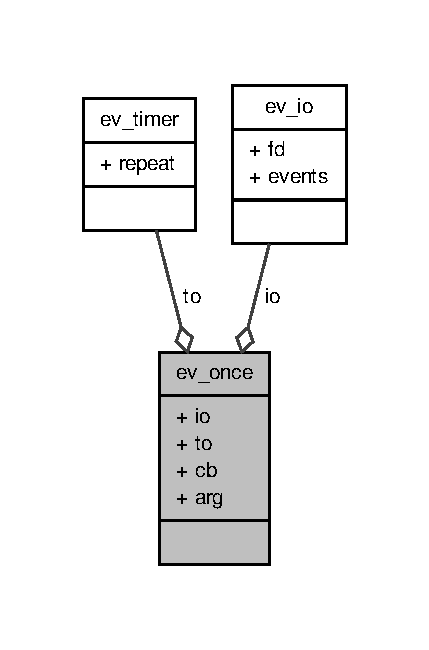
\includegraphics[width=206pt]{structev__once__coll__graph}
\end{center}
\end{figure}
\subsection*{\-Data \-Fields}
\begin{DoxyCompactItemize}
\item 
\hyperlink{structev__io}{ev\-\_\-io} \hyperlink{structev__once_a0a60f96152fbb4f3d01c7ef3e4a3d856}{io}
\item 
\hyperlink{structev__timer}{ev\-\_\-timer} \hyperlink{structev__once_a07c6e8b8c00f07a7dcad174eb9b0a9e8}{to}
\item 
void($\ast$ \hyperlink{structev__once_ade289570a63e50d9a874027c1f34f0ff}{cb} )(int revents, void $\ast$\hyperlink{structev__once_a9ce2ec4812a92cb6ab39f6e81e9173a9}{arg})
\item 
void $\ast$ \hyperlink{structev__once_a9ce2ec4812a92cb6ab39f6e81e9173a9}{arg}
\end{DoxyCompactItemize}


\subsection{\-Detailed \-Description}


\-Definition at line 4713 of file ev.\-c.



\subsection{\-Field \-Documentation}
\hypertarget{structev__once_a9ce2ec4812a92cb6ab39f6e81e9173a9}{\index{ev\-\_\-once@{ev\-\_\-once}!arg@{arg}}
\index{arg@{arg}!ev_once@{ev\-\_\-once}}
\subsubsection[{arg}]{\setlength{\rightskip}{0pt plus 5cm}void$\ast$ {\bf arg}}}\label{structev__once_a9ce2ec4812a92cb6ab39f6e81e9173a9}


\-Definition at line 4718 of file ev.\-c.

\hypertarget{structev__once_ade289570a63e50d9a874027c1f34f0ff}{\index{ev\-\_\-once@{ev\-\_\-once}!cb@{cb}}
\index{cb@{cb}!ev_once@{ev\-\_\-once}}
\subsubsection[{cb}]{\setlength{\rightskip}{0pt plus 5cm}void($\ast$ {\bf cb})(int revents, void $\ast${\bf arg})}}\label{structev__once_ade289570a63e50d9a874027c1f34f0ff}


\-Definition at line 4717 of file ev.\-c.

\hypertarget{structev__once_a0a60f96152fbb4f3d01c7ef3e4a3d856}{\index{ev\-\_\-once@{ev\-\_\-once}!io@{io}}
\index{io@{io}!ev_once@{ev\-\_\-once}}
\subsubsection[{io}]{\setlength{\rightskip}{0pt plus 5cm}{\bf ev\-\_\-io} {\bf io}}}\label{structev__once_a0a60f96152fbb4f3d01c7ef3e4a3d856}


\-Definition at line 4715 of file ev.\-c.

\hypertarget{structev__once_a07c6e8b8c00f07a7dcad174eb9b0a9e8}{\index{ev\-\_\-once@{ev\-\_\-once}!to@{to}}
\index{to@{to}!ev_once@{ev\-\_\-once}}
\subsubsection[{to}]{\setlength{\rightskip}{0pt plus 5cm}{\bf ev\-\_\-timer} {\bf to}}}\label{structev__once_a07c6e8b8c00f07a7dcad174eb9b0a9e8}


\-Definition at line 4716 of file ev.\-c.



\-The documentation for this struct was generated from the following file\-:\begin{DoxyCompactItemize}
\item 
/home/jaymiao/workstation/github/libev-\/4.\-19/\hyperlink{ev_8c}{ev.\-c}\end{DoxyCompactItemize}

\hypertarget{structev__periodic}{\section{ev\-\_\-periodic \-Struct \-Reference}
\label{structev__periodic}\index{ev\-\_\-periodic@{ev\-\_\-periodic}}
}


{\ttfamily \#include $<$ev.\-h$>$}

\subsection*{\-Data \-Fields}
\begin{DoxyCompactItemize}
\item 
\hyperlink{ev_8h_add71e34ce2b04bbf7eb6f31a850814e8}{ev\-\_\-tstamp} \hyperlink{structev__periodic_ac00ce9c33f0c138a374ae6d957434253}{offset}
\item 
\hyperlink{ev_8h_add71e34ce2b04bbf7eb6f31a850814e8}{ev\-\_\-tstamp} \hyperlink{structev__periodic_a710c94a682e5e9281b2e5162e265b726}{interval}
\item 
\hyperlink{ev_8h_add71e34ce2b04bbf7eb6f31a850814e8}{ev\-\_\-tstamp}($\ast$ \hyperlink{structev__periodic_a9db54a5bc43f82d7d1b46be67a2115eb}{reschedule\-\_\-cb} )(struct \hyperlink{structev__periodic}{ev\-\_\-periodic} $\ast$w, \hyperlink{ev_8h_add71e34ce2b04bbf7eb6f31a850814e8}{ev\-\_\-tstamp} now) \hyperlink{ev_8h_a473b5b606fdd3d484227542605e80bcf}{\-E\-V\-\_\-\-T\-H\-R\-O\-W}
\end{DoxyCompactItemize}


\subsection{\-Detailed \-Description}


\-Definition at line 330 of file ev.\-h.



\subsection{\-Field \-Documentation}
\hypertarget{structev__periodic_a710c94a682e5e9281b2e5162e265b726}{\index{ev\-\_\-periodic@{ev\-\_\-periodic}!interval@{interval}}
\index{interval@{interval}!ev_periodic@{ev\-\_\-periodic}}
\subsubsection[{interval}]{\setlength{\rightskip}{0pt plus 5cm}{\bf ev\-\_\-tstamp} {\bf interval}}}\label{structev__periodic_a710c94a682e5e9281b2e5162e265b726}


\-Definition at line 335 of file ev.\-h.

\hypertarget{structev__periodic_ac00ce9c33f0c138a374ae6d957434253}{\index{ev\-\_\-periodic@{ev\-\_\-periodic}!offset@{offset}}
\index{offset@{offset}!ev_periodic@{ev\-\_\-periodic}}
\subsubsection[{offset}]{\setlength{\rightskip}{0pt plus 5cm}{\bf ev\-\_\-tstamp} {\bf offset}}}\label{structev__periodic_ac00ce9c33f0c138a374ae6d957434253}


\-Definition at line 334 of file ev.\-h.

\hypertarget{structev__periodic_a9db54a5bc43f82d7d1b46be67a2115eb}{\index{ev\-\_\-periodic@{ev\-\_\-periodic}!reschedule\-\_\-cb@{reschedule\-\_\-cb}}
\index{reschedule\-\_\-cb@{reschedule\-\_\-cb}!ev_periodic@{ev\-\_\-periodic}}
\subsubsection[{reschedule\-\_\-cb}]{\setlength{\rightskip}{0pt plus 5cm}{\bf ev\-\_\-tstamp}($\ast$ {\bf reschedule\-\_\-cb})(struct {\bf ev\-\_\-periodic} $\ast$w, {\bf ev\-\_\-tstamp} now) {\bf \-E\-V\-\_\-\-T\-H\-R\-O\-W}}}\label{structev__periodic_a9db54a5bc43f82d7d1b46be67a2115eb}


\-Definition at line 336 of file ev.\-h.



\-The documentation for this struct was generated from the following file\-:\begin{DoxyCompactItemize}
\item 
/home/jaymiao/workstation/github/libev-\/4.\-19/\hyperlink{ev_8h}{ev.\-h}\end{DoxyCompactItemize}

\hypertarget{structev__prepare}{\section{ev\-\_\-prepare \-Struct \-Reference}
\label{structev__prepare}\index{ev\-\_\-prepare@{ev\-\_\-prepare}}
}


{\ttfamily \#include $<$ev.\-h$>$}



\subsection{\-Detailed \-Description}


\-Definition at line 397 of file ev.\-h.



\-The documentation for this struct was generated from the following file\-:\begin{DoxyCompactItemize}
\item 
/home/jaymiao/workstation/github/libev-\/4.\-19/\hyperlink{ev_8h}{ev.\-h}\end{DoxyCompactItemize}

\hypertarget{structev__signal}{\section{ev\-\_\-signal \-Struct \-Reference}
\label{structev__signal}\index{ev\-\_\-signal@{ev\-\_\-signal}}
}


{\ttfamily \#include $<$ev.\-h$>$}

\subsection*{\-Data \-Fields}
\begin{DoxyCompactItemize}
\item 
int \hyperlink{structev__signal_af063222f46f5e774717f2f0a077302af}{signum}
\end{DoxyCompactItemize}


\subsection{\-Detailed \-Description}


\-Definition at line 341 of file ev.\-h.



\subsection{\-Field \-Documentation}
\hypertarget{structev__signal_af063222f46f5e774717f2f0a077302af}{\index{ev\-\_\-signal@{ev\-\_\-signal}!signum@{signum}}
\index{signum@{signum}!ev_signal@{ev\-\_\-signal}}
\subsubsection[{signum}]{\setlength{\rightskip}{0pt plus 5cm}int {\bf signum}}}\label{structev__signal_af063222f46f5e774717f2f0a077302af}


\-Definition at line 345 of file ev.\-h.



\-The documentation for this struct was generated from the following file\-:\begin{DoxyCompactItemize}
\item 
/home/jaymiao/workstation/github/libev-\/4.\-19/\hyperlink{ev_8h}{ev.\-h}\end{DoxyCompactItemize}

\hypertarget{structev__stat}{\section{ev\-\_\-stat \-Struct \-Reference}
\label{structev__stat}\index{ev\-\_\-stat@{ev\-\_\-stat}}
}


{\ttfamily \#include $<$ev.\-h$>$}



\-Collaboration diagram for ev\-\_\-stat\-:
\nopagebreak
\begin{figure}[H]
\begin{center}
\leavevmode
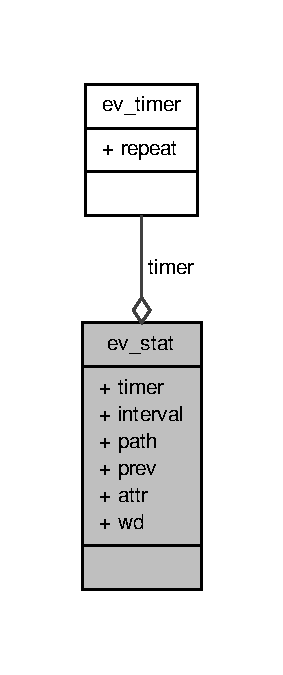
\includegraphics[width=136pt]{structev__stat__coll__graph}
\end{center}
\end{figure}
\subsection*{\-Data \-Fields}
\begin{DoxyCompactItemize}
\item 
\hyperlink{structev__timer}{ev\-\_\-timer} \hyperlink{structev__stat_a56d2f62405e7a2bba42204f714803c7c}{timer}
\item 
\hyperlink{ev_8h_add71e34ce2b04bbf7eb6f31a850814e8}{ev\-\_\-tstamp} \hyperlink{structev__stat_a710c94a682e5e9281b2e5162e265b726}{interval}
\item 
const char $\ast$ \hyperlink{structev__stat_a3b02c6de5c049804444a246f7fdf46b4}{path}
\item 
\hyperlink{ev_8h_af7665657cb718a911fd591bc0613db83}{ev\-\_\-statdata} \hyperlink{structev__stat_a02b7b656210f66c84f0b28cf3f4c745d}{prev}
\item 
\hyperlink{ev_8h_af7665657cb718a911fd591bc0613db83}{ev\-\_\-statdata} \hyperlink{structev__stat_a597fb418c2fd88ae12847805bddbe09d}{attr}
\item 
int \hyperlink{structev__stat_a3707c399a8d778793ccd2c311867ac44}{wd}
\end{DoxyCompactItemize}


\subsection{\-Detailed \-Description}


\-Definition at line 371 of file ev.\-h.



\subsection{\-Field \-Documentation}
\hypertarget{structev__stat_a597fb418c2fd88ae12847805bddbe09d}{\index{ev\-\_\-stat@{ev\-\_\-stat}!attr@{attr}}
\index{attr@{attr}!ev_stat@{ev\-\_\-stat}}
\subsubsection[{attr}]{\setlength{\rightskip}{0pt plus 5cm}{\bf ev\-\_\-statdata} {\bf attr}}}\label{structev__stat_a597fb418c2fd88ae12847805bddbe09d}


\-Definition at line 379 of file ev.\-h.

\hypertarget{structev__stat_a710c94a682e5e9281b2e5162e265b726}{\index{ev\-\_\-stat@{ev\-\_\-stat}!interval@{interval}}
\index{interval@{interval}!ev_stat@{ev\-\_\-stat}}
\subsubsection[{interval}]{\setlength{\rightskip}{0pt plus 5cm}{\bf ev\-\_\-tstamp} {\bf interval}}}\label{structev__stat_a710c94a682e5e9281b2e5162e265b726}


\-Definition at line 376 of file ev.\-h.

\hypertarget{structev__stat_a3b02c6de5c049804444a246f7fdf46b4}{\index{ev\-\_\-stat@{ev\-\_\-stat}!path@{path}}
\index{path@{path}!ev_stat@{ev\-\_\-stat}}
\subsubsection[{path}]{\setlength{\rightskip}{0pt plus 5cm}const char$\ast$ {\bf path}}}\label{structev__stat_a3b02c6de5c049804444a246f7fdf46b4}


\-Definition at line 377 of file ev.\-h.

\hypertarget{structev__stat_a02b7b656210f66c84f0b28cf3f4c745d}{\index{ev\-\_\-stat@{ev\-\_\-stat}!prev@{prev}}
\index{prev@{prev}!ev_stat@{ev\-\_\-stat}}
\subsubsection[{prev}]{\setlength{\rightskip}{0pt plus 5cm}{\bf ev\-\_\-statdata} {\bf prev}}}\label{structev__stat_a02b7b656210f66c84f0b28cf3f4c745d}


\-Definition at line 378 of file ev.\-h.

\hypertarget{structev__stat_a56d2f62405e7a2bba42204f714803c7c}{\index{ev\-\_\-stat@{ev\-\_\-stat}!timer@{timer}}
\index{timer@{timer}!ev_stat@{ev\-\_\-stat}}
\subsubsection[{timer}]{\setlength{\rightskip}{0pt plus 5cm}{\bf ev\-\_\-timer} {\bf timer}}}\label{structev__stat_a56d2f62405e7a2bba42204f714803c7c}


\-Definition at line 375 of file ev.\-h.

\hypertarget{structev__stat_a3707c399a8d778793ccd2c311867ac44}{\index{ev\-\_\-stat@{ev\-\_\-stat}!wd@{wd}}
\index{wd@{wd}!ev_stat@{ev\-\_\-stat}}
\subsubsection[{wd}]{\setlength{\rightskip}{0pt plus 5cm}int {\bf wd}}}\label{structev__stat_a3707c399a8d778793ccd2c311867ac44}


\-Definition at line 381 of file ev.\-h.



\-The documentation for this struct was generated from the following file\-:\begin{DoxyCompactItemize}
\item 
/home/jaymiao/workstation/github/libev-\/4.\-19/\hyperlink{ev_8h}{ev.\-h}\end{DoxyCompactItemize}

\hypertarget{structev__timer}{\section{ev\-\_\-timer \-Struct \-Reference}
\label{structev__timer}\index{ev\-\_\-timer@{ev\-\_\-timer}}
}


{\ttfamily \#include $<$ev.\-h$>$}

\subsection*{\-Data \-Fields}
\begin{DoxyCompactItemize}
\item 
\hyperlink{ev_8h_add71e34ce2b04bbf7eb6f31a850814e8}{ev\-\_\-tstamp} \hyperlink{structev__timer_a6113423f01aea60101124c80ace1df52}{repeat}
\end{DoxyCompactItemize}


\subsection{\-Detailed \-Description}


\-Definition at line 321 of file ev.\-h.



\subsection{\-Field \-Documentation}
\hypertarget{structev__timer_a6113423f01aea60101124c80ace1df52}{\index{ev\-\_\-timer@{ev\-\_\-timer}!repeat@{repeat}}
\index{repeat@{repeat}!ev_timer@{ev\-\_\-timer}}
\subsubsection[{repeat}]{\setlength{\rightskip}{0pt plus 5cm}{\bf ev\-\_\-tstamp} {\bf repeat}}}\label{structev__timer_a6113423f01aea60101124c80ace1df52}


\-Definition at line 325 of file ev.\-h.



\-The documentation for this struct was generated from the following file\-:\begin{DoxyCompactItemize}
\item 
/home/jaymiao/workstation/github/libev-\/4.\-19/\hyperlink{ev_8h}{ev.\-h}\end{DoxyCompactItemize}

\hypertarget{structev__watcher}{\section{ev\-\_\-watcher \-Struct \-Reference}
\label{structev__watcher}\index{ev\-\_\-watcher@{ev\-\_\-watcher}}
}


{\ttfamily \#include $<$ev.\-h$>$}



\-Inheritance diagram for ev\-\_\-watcher\-:
\nopagebreak
\begin{figure}[H]
\begin{center}
\leavevmode
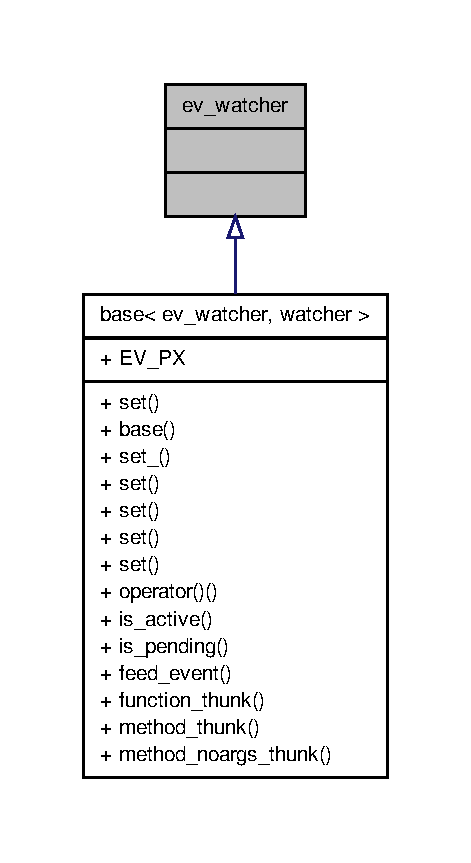
\includegraphics[width=226pt]{structev__watcher__inherit__graph}
\end{center}
\end{figure}


\subsection{\-Detailed \-Description}


\-Definition at line 292 of file ev.\-h.



\-The documentation for this struct was generated from the following file\-:\begin{DoxyCompactItemize}
\item 
/home/jaymiao/workstation/github/libev-\/4.\-19/\hyperlink{ev_8h}{ev.\-h}\end{DoxyCompactItemize}

\hypertarget{structev__watcher__list}{\section{ev\-\_\-watcher\-\_\-list \-Struct \-Reference}
\label{structev__watcher__list}\index{ev\-\_\-watcher\-\_\-list@{ev\-\_\-watcher\-\_\-list}}
}


{\ttfamily \#include $<$ev.\-h$>$}



\subsection{\-Detailed \-Description}


\-Definition at line 298 of file ev.\-h.



\-The documentation for this struct was generated from the following file\-:\begin{DoxyCompactItemize}
\item 
/home/jaymiao/workstation/github/libev-\/4.\-19/\hyperlink{ev_8h}{ev.\-h}\end{DoxyCompactItemize}

\hypertarget{structev__watcher__time}{\section{ev\-\_\-watcher\-\_\-time \-Struct \-Reference}
\label{structev__watcher__time}\index{ev\-\_\-watcher\-\_\-time@{ev\-\_\-watcher\-\_\-time}}
}


{\ttfamily \#include $<$ev.\-h$>$}



\subsection{\-Detailed \-Description}


\-Definition at line 304 of file ev.\-h.



\-The documentation for this struct was generated from the following file\-:\begin{DoxyCompactItemize}
\item 
/home/jaymiao/workstation/github/libev-\/4.\-19/\hyperlink{ev_8h}{ev.\-h}\end{DoxyCompactItemize}

\hypertarget{structev__x__once}{\section{ev\-\_\-x\-\_\-once \-Struct \-Reference}
\label{structev__x__once}\index{ev\-\_\-x\-\_\-once@{ev\-\_\-x\-\_\-once}}
}
\subsection*{\-Data \-Fields}
\begin{DoxyCompactItemize}
\item 
int \hyperlink{structev__x__once_a6f8059414f0228f0256115e024eeed4b}{fd}
\item 
void($\ast$ \hyperlink{structev__x__once_a5e20cc2d3b4d4967380f263227acc60c}{cb} )(int, short, void $\ast$)
\item 
void $\ast$ \hyperlink{structev__x__once_a9ce2ec4812a92cb6ab39f6e81e9173a9}{arg}
\end{DoxyCompactItemize}


\subsection{\-Detailed \-Description}


\-Definition at line 386 of file event.\-c.



\subsection{\-Field \-Documentation}
\hypertarget{structev__x__once_a9ce2ec4812a92cb6ab39f6e81e9173a9}{\index{ev\-\_\-x\-\_\-once@{ev\-\_\-x\-\_\-once}!arg@{arg}}
\index{arg@{arg}!ev_x_once@{ev\-\_\-x\-\_\-once}}
\subsubsection[{arg}]{\setlength{\rightskip}{0pt plus 5cm}void$\ast$ {\bf arg}}}\label{structev__x__once_a9ce2ec4812a92cb6ab39f6e81e9173a9}


\-Definition at line 390 of file event.\-c.

\hypertarget{structev__x__once_a5e20cc2d3b4d4967380f263227acc60c}{\index{ev\-\_\-x\-\_\-once@{ev\-\_\-x\-\_\-once}!cb@{cb}}
\index{cb@{cb}!ev_x_once@{ev\-\_\-x\-\_\-once}}
\subsubsection[{cb}]{\setlength{\rightskip}{0pt plus 5cm}void($\ast$ {\bf cb})(int, short, void $\ast$)}}\label{structev__x__once_a5e20cc2d3b4d4967380f263227acc60c}


\-Definition at line 389 of file event.\-c.

\hypertarget{structev__x__once_a6f8059414f0228f0256115e024eeed4b}{\index{ev\-\_\-x\-\_\-once@{ev\-\_\-x\-\_\-once}!fd@{fd}}
\index{fd@{fd}!ev_x_once@{ev\-\_\-x\-\_\-once}}
\subsubsection[{fd}]{\setlength{\rightskip}{0pt plus 5cm}int {\bf fd}}}\label{structev__x__once_a6f8059414f0228f0256115e024eeed4b}


\-Definition at line 388 of file event.\-c.



\-The documentation for this struct was generated from the following file\-:\begin{DoxyCompactItemize}
\item 
/home/jaymiao/workstation/github/libev-\/4.\-19/\hyperlink{event_8c}{event.\-c}\end{DoxyCompactItemize}

\hypertarget{structevent}{\section{event \-Struct \-Reference}
\label{structevent}\index{event@{event}}
}


{\ttfamily \#include $<$event.\-h$>$}



\-Collaboration diagram for event\-:
\nopagebreak
\begin{figure}[H]
\begin{center}
\leavevmode
\includegraphics[width=350pt]{structevent__coll__graph}
\end{center}
\end{figure}
\subsection*{\-Data \-Fields}
\begin{DoxyCompactItemize}
\item 
\begin{tabbing}
xx\=xx\=xx\=xx\=xx\=xx\=xx\=xx\=xx\=\kill
union \{\\
\>struct \hyperlink{structev__io}{ev\_io} \hyperlink{structevent_a8a4fa321488e67a96ad783dc24187c4c}{io}\\
\>struct \hyperlink{structev__signal}{ev\_signal} \hyperlink{structevent_ad3d5a2f9ab72029d05b260267e08eba1}{sig}\\
\} \hyperlink{structevent_a3fbb6fe0300dadbfebf8d1516f74082d}{iosig}\\

\end{tabbing}\item 
struct \hyperlink{structev__timer}{ev\-\_\-timer} \hyperlink{structevent_aba52a2d8ebe3e4d2e9bac349f661d509}{to}
\item 
struct \hyperlink{structevent__base}{event\-\_\-base} $\ast$ \hyperlink{structevent_a79005f93f769baaa5ab5d2a45b52ec62}{ev\-\_\-base}
\item 
\hyperlink{event_8h_a675c7b1b04923fb1b48f758222ab1333}{event\-\_\-callback\-\_\-fn} \hyperlink{structevent_a420d7cc7bf56d48aeeb1e27b52d7c829}{ev\-\_\-callback}
\item 
void $\ast$ \hyperlink{structevent_a680e2f70d6e4ce56b58f57e1182ffac1}{ev\-\_\-arg}
\item 
int \hyperlink{structevent_a7016497f14046277c71be6d4c1620890}{ev\-\_\-fd}
\item 
int \hyperlink{structevent_afc1b09b76d937eb994d6cdd3adf9ffcc}{ev\-\_\-pri}
\item 
int \hyperlink{structevent_acea2638a9075ad5d22ee179fda2fb8bc}{ev\-\_\-res}
\item 
int \hyperlink{structevent_a7facfe0f28541f092cd123c21e89c6c4}{ev\-\_\-flags}
\item 
short \hyperlink{structevent_a1c8a838880f1938d9ea23dcfee0419ea}{ev\-\_\-events}
\end{DoxyCompactItemize}


\subsection{\-Detailed \-Description}


\-Definition at line 80 of file event.\-h.



\subsection{\-Field \-Documentation}
\hypertarget{structevent_a680e2f70d6e4ce56b58f57e1182ffac1}{\index{event@{event}!ev\-\_\-arg@{ev\-\_\-arg}}
\index{ev\-\_\-arg@{ev\-\_\-arg}!event@{event}}
\subsubsection[{ev\-\_\-arg}]{\setlength{\rightskip}{0pt plus 5cm}void$\ast$ {\bf ev\-\_\-arg}}}\label{structevent_a680e2f70d6e4ce56b58f57e1182ffac1}


\-Definition at line 92 of file event.\-h.

\hypertarget{structevent_a79005f93f769baaa5ab5d2a45b52ec62}{\index{event@{event}!ev\-\_\-base@{ev\-\_\-base}}
\index{ev\-\_\-base@{ev\-\_\-base}!event@{event}}
\subsubsection[{ev\-\_\-base}]{\setlength{\rightskip}{0pt plus 5cm}struct {\bf event\-\_\-base}$\ast$ {\bf ev\-\_\-base}}}\label{structevent_a79005f93f769baaa5ab5d2a45b52ec62}


\-Definition at line 90 of file event.\-h.

\hypertarget{structevent_a420d7cc7bf56d48aeeb1e27b52d7c829}{\index{event@{event}!ev\-\_\-callback@{ev\-\_\-callback}}
\index{ev\-\_\-callback@{ev\-\_\-callback}!event@{event}}
\subsubsection[{ev\-\_\-callback}]{\setlength{\rightskip}{0pt plus 5cm}{\bf event\-\_\-callback\-\_\-fn} {\bf ev\-\_\-callback}}}\label{structevent_a420d7cc7bf56d48aeeb1e27b52d7c829}


\-Definition at line 91 of file event.\-h.

\hypertarget{structevent_a1c8a838880f1938d9ea23dcfee0419ea}{\index{event@{event}!ev\-\_\-events@{ev\-\_\-events}}
\index{ev\-\_\-events@{ev\-\_\-events}!event@{event}}
\subsubsection[{ev\-\_\-events}]{\setlength{\rightskip}{0pt plus 5cm}short {\bf ev\-\_\-events}}}\label{structevent_a1c8a838880f1938d9ea23dcfee0419ea}


\-Definition at line 97 of file event.\-h.

\hypertarget{structevent_a7016497f14046277c71be6d4c1620890}{\index{event@{event}!ev\-\_\-fd@{ev\-\_\-fd}}
\index{ev\-\_\-fd@{ev\-\_\-fd}!event@{event}}
\subsubsection[{ev\-\_\-fd}]{\setlength{\rightskip}{0pt plus 5cm}int {\bf ev\-\_\-fd}}}\label{structevent_a7016497f14046277c71be6d4c1620890}


\-Definition at line 93 of file event.\-h.

\hypertarget{structevent_a7facfe0f28541f092cd123c21e89c6c4}{\index{event@{event}!ev\-\_\-flags@{ev\-\_\-flags}}
\index{ev\-\_\-flags@{ev\-\_\-flags}!event@{event}}
\subsubsection[{ev\-\_\-flags}]{\setlength{\rightskip}{0pt plus 5cm}int {\bf ev\-\_\-flags}}}\label{structevent_a7facfe0f28541f092cd123c21e89c6c4}


\-Definition at line 96 of file event.\-h.

\hypertarget{structevent_afc1b09b76d937eb994d6cdd3adf9ffcc}{\index{event@{event}!ev\-\_\-pri@{ev\-\_\-pri}}
\index{ev\-\_\-pri@{ev\-\_\-pri}!event@{event}}
\subsubsection[{ev\-\_\-pri}]{\setlength{\rightskip}{0pt plus 5cm}int {\bf ev\-\_\-pri}}}\label{structevent_afc1b09b76d937eb994d6cdd3adf9ffcc}


\-Definition at line 94 of file event.\-h.

\hypertarget{structevent_acea2638a9075ad5d22ee179fda2fb8bc}{\index{event@{event}!ev\-\_\-res@{ev\-\_\-res}}
\index{ev\-\_\-res@{ev\-\_\-res}!event@{event}}
\subsubsection[{ev\-\_\-res}]{\setlength{\rightskip}{0pt plus 5cm}int {\bf ev\-\_\-res}}}\label{structevent_acea2638a9075ad5d22ee179fda2fb8bc}


\-Definition at line 95 of file event.\-h.

\hypertarget{structevent_a8a4fa321488e67a96ad783dc24187c4c}{\index{event@{event}!io@{io}}
\index{io@{io}!event@{event}}
\subsubsection[{io}]{\setlength{\rightskip}{0pt plus 5cm}struct {\bf ev\-\_\-io} {\bf io}}}\label{structevent_a8a4fa321488e67a96ad783dc24187c4c}


\-Definition at line 84 of file event.\-h.

\hypertarget{structevent_a3fbb6fe0300dadbfebf8d1516f74082d}{\index{event@{event}!iosig@{iosig}}
\index{iosig@{iosig}!event@{event}}
\subsubsection[{iosig}]{\setlength{\rightskip}{0pt plus 5cm}union \{ ... \}   {\bf iosig}}}\label{structevent_a3fbb6fe0300dadbfebf8d1516f74082d}
\hypertarget{structevent_ad3d5a2f9ab72029d05b260267e08eba1}{\index{event@{event}!sig@{sig}}
\index{sig@{sig}!event@{event}}
\subsubsection[{sig}]{\setlength{\rightskip}{0pt plus 5cm}struct {\bf ev\-\_\-signal} {\bf sig}}}\label{structevent_ad3d5a2f9ab72029d05b260267e08eba1}


\-Definition at line 85 of file event.\-h.

\hypertarget{structevent_aba52a2d8ebe3e4d2e9bac349f661d509}{\index{event@{event}!to@{to}}
\index{to@{to}!event@{event}}
\subsubsection[{to}]{\setlength{\rightskip}{0pt plus 5cm}struct {\bf ev\-\_\-timer} {\bf to}}}\label{structevent_aba52a2d8ebe3e4d2e9bac349f661d509}


\-Definition at line 87 of file event.\-h.



\-The documentation for this struct was generated from the following file\-:\begin{DoxyCompactItemize}
\item 
/home/jaymiao/workstation/github/libev-\/4.\-19/\hyperlink{event_8h}{event.\-h}\end{DoxyCompactItemize}

\hypertarget{structevent__base}{\section{event\-\_\-base \-Struct \-Reference}
\label{structevent__base}\index{event\-\_\-base@{event\-\_\-base}}
}
\subsection*{\-Data \-Fields}
\begin{DoxyCompactItemize}
\item 
int \hyperlink{structevent__base_a7c1d654b7b6114d7a0abc8d351dd1bcd}{dummy}
\end{DoxyCompactItemize}


\subsection{\-Detailed \-Description}


\-Definition at line 59 of file event.\-c.



\subsection{\-Field \-Documentation}
\hypertarget{structevent__base_a7c1d654b7b6114d7a0abc8d351dd1bcd}{\index{event\-\_\-base@{event\-\_\-base}!dummy@{dummy}}
\index{dummy@{dummy}!event_base@{event\-\_\-base}}
\subsubsection[{dummy}]{\setlength{\rightskip}{0pt plus 5cm}int {\bf dummy}}}\label{structevent__base_a7c1d654b7b6114d7a0abc8d351dd1bcd}


\-Definition at line 61 of file event.\-c.



\-The documentation for this struct was generated from the following file\-:\begin{DoxyCompactItemize}
\item 
/home/jaymiao/workstation/github/libev-\/4.\-19/\hyperlink{event_8c}{event.\-c}\end{DoxyCompactItemize}

\hypertarget{structev_1_1loop__ref}{\section{loop\-\_\-ref \-Struct \-Reference}
\label{structev_1_1loop__ref}\index{loop\-\_\-ref@{loop\-\_\-ref}}
}


{\ttfamily \#include $<$ev++.\-h$>$}



\-Inheritance diagram for loop\-\_\-ref\-:
\nopagebreak
\begin{figure}[H]
\begin{center}
\leavevmode
\includegraphics[width=280pt]{structev_1_1loop__ref__inherit__graph}
\end{center}
\end{figure}


\-Collaboration diagram for loop\-\_\-ref\-:
\nopagebreak
\begin{figure}[H]
\begin{center}
\leavevmode
\includegraphics[height=550pt]{structev_1_1loop__ref__coll__graph}
\end{center}
\end{figure}
\subsection*{\-Public \-Member \-Functions}
\begin{DoxyCompactItemize}
\item 
\hyperlink{structev_1_1loop__ref_a6dee3b5f76ff45ed7bc33d1cbab089d4}{loop\-\_\-ref} (\hyperlink{ev_8h_a6e6c6b499d18513c01cf4bde00121617}{\-E\-V\-\_\-\-P})  throw ()
\item 
bool \hyperlink{structev_1_1loop__ref_a1f090cb316333b2c1648df9e160e2ad6}{operator==} (const \hyperlink{structev_1_1loop__ref}{loop\-\_\-ref} \&other) const   throw ()
\item 
bool \hyperlink{structev_1_1loop__ref_aebe64584aeb2fb24a3a3a9bcfa13eebf}{operator!=} (const \hyperlink{structev_1_1loop__ref}{loop\-\_\-ref} \&other) const   throw ()
\item 
bool \hyperlink{structev_1_1loop__ref_a8d7e20431148d5493bc9c2315840bebb}{operator==} (const \hyperlink{ev_8h_a6e6c6b499d18513c01cf4bde00121617}{\-E\-V\-\_\-\-P}) const   throw ()
\item 
bool \hyperlink{structev_1_1loop__ref_aca6d051b2096bc358dfb6625d1b9aebb}{operator!=} (const \hyperlink{ev_8h_a6e6c6b499d18513c01cf4bde00121617}{\-E\-V\-\_\-\-P}) const   throw ()
\item 
\hyperlink{structev_1_1loop__ref_af995b1dfab9287f0f3a98d8134cfd974}{operator struct ev\-\_\-loop $\ast$} () const   throw ()
\item 
\hyperlink{structev_1_1loop__ref_a13b88541123e99d2782cd6c81101417d}{operator const struct ev\-\_\-loop $\ast$} () const   throw ()
\item 
bool \hyperlink{structev_1_1loop__ref_aa9b92fe88733a9bd5be8b42301459b13}{is\-\_\-default} () const   throw ()
\item 
void \hyperlink{structev_1_1loop__ref_a52fa73aeb9b8f6319d2041baf5a8bd58}{loop} (int flags=0)
\item 
void \hyperlink{structev_1_1loop__ref_af629d4578522c4f65e29b0b57249889e}{unloop} (\hyperlink{namespaceev_aca7e42bfd95674ad51c82b41e0c3329e}{how\-\_\-t} how=\hyperlink{namespaceev_aca7e42bfd95674ad51c82b41e0c3329ea7a725f13af144bdef532d0389ba75e0d}{\-O\-N\-E})  throw ()
\item 
void \hyperlink{structev_1_1loop__ref_a64fe8b8a12ce7308a7f5fb9399d36757}{run} (int flags=0)
\item 
void \hyperlink{structev_1_1loop__ref_a1f85df7d48620ed7aefb863acb7167ad}{break\-\_\-loop} (\hyperlink{namespaceev_aca7e42bfd95674ad51c82b41e0c3329e}{how\-\_\-t} how=\hyperlink{namespaceev_aca7e42bfd95674ad51c82b41e0c3329ea7a725f13af144bdef532d0389ba75e0d}{\-O\-N\-E})  throw ()
\item 
void \hyperlink{structev_1_1loop__ref_a974a8c58270dc360e96f567d31a7176e}{post\-\_\-fork} ()  throw ()
\item 
unsigned int \hyperlink{structev_1_1loop__ref_ae47173b96e5b1a587c38070bfe78d98a}{backend} () const   throw ()
\item 
\hyperlink{namespaceev_a9853823b701944a8a5ce179d10a24b97}{tstamp} \hyperlink{structev_1_1loop__ref_a98d982e3931bfdd1e920dd577db61c31}{now} () const   throw ()
\item 
void \hyperlink{structev_1_1loop__ref_ae84429cc5d55e687f3abbd5c0bfe7430}{ref} ()  throw ()
\item 
void \hyperlink{structev_1_1loop__ref_abe058b11156f019666c15a53a3fa7218}{unref} ()  throw ()
\item 
unsigned int \hyperlink{structev_1_1loop__ref_a2b3d64162433abbd749e2722926fb0b5}{iteration} () const   throw ()
\item 
unsigned int \hyperlink{structev_1_1loop__ref_a38a6400670c0b7da8bf9523a22d68692}{depth} () const   throw ()
\item 
void \hyperlink{structev_1_1loop__ref_aeace41f14b7d95fa116a81298ab0d058}{set\-\_\-io\-\_\-collect\-\_\-interval} (\hyperlink{namespaceev_a9853823b701944a8a5ce179d10a24b97}{tstamp} interval)  throw ()
\item 
void \hyperlink{structev_1_1loop__ref_aa29b4b76ece69d4dea9509a2cf827a6c}{set\-\_\-timeout\-\_\-collect\-\_\-interval} (\hyperlink{namespaceev_a9853823b701944a8a5ce179d10a24b97}{tstamp} interval)  throw ()
\item 
void \hyperlink{structev_1_1loop__ref_a5cd55f27ad5ce7084be26022d3dc6628}{once} (int fd, int events, \hyperlink{namespaceev_a9853823b701944a8a5ce179d10a24b97}{tstamp} timeout, void($\ast$cb)(int, void $\ast$), void $\ast$arg=0)  throw ()
\item 
{\footnotesize template$<$class K , void(\-K\-::$\ast$)(int) method$>$ }\\void \hyperlink{structev_1_1loop__ref_aecce9953b684e4b8db13b3a9d82520ca}{once} (int fd, int events, \hyperlink{namespaceev_a9853823b701944a8a5ce179d10a24b97}{tstamp} timeout, \-K $\ast$object)  throw ()
\item 
{\footnotesize template$<$class K $>$ }\\void \hyperlink{structev_1_1loop__ref_ae3a77041d3c6ae893f0573000cac252a}{once} (int fd, int events, \hyperlink{namespaceev_a9853823b701944a8a5ce179d10a24b97}{tstamp} timeout, \-K $\ast$object)  throw ()
\item 
{\footnotesize template$<$class K , void(\-K\-::$\ast$)() method$>$ }\\void \hyperlink{structev_1_1loop__ref_aecce9953b684e4b8db13b3a9d82520ca}{once} (int fd, int events, \hyperlink{namespaceev_a9853823b701944a8a5ce179d10a24b97}{tstamp} timeout, \-K $\ast$object)  throw ()
\item 
{\footnotesize template$<$void($\ast$)(int) cb$>$ }\\void \hyperlink{structev_1_1loop__ref_a5a68aa8f7554b9aab364abce41180d84}{once} (int fd, int events, \hyperlink{namespaceev_a9853823b701944a8a5ce179d10a24b97}{tstamp} timeout)  throw ()
\item 
{\footnotesize template$<$void($\ast$)() cb$>$ }\\void \hyperlink{structev_1_1loop__ref_a5a68aa8f7554b9aab364abce41180d84}{once} (int fd, int events, \hyperlink{namespaceev_a9853823b701944a8a5ce179d10a24b97}{tstamp} timeout)  throw ()
\item 
void \hyperlink{structev_1_1loop__ref_a583fb6668c11d14b9e9a5495b5664656}{feed\-\_\-fd\-\_\-event} (int fd, int revents)  throw ()
\item 
void \hyperlink{structev_1_1loop__ref_ab64972f5cac053e4f240d8cb3bace62e}{feed\-\_\-signal\-\_\-event} (int signum)  throw ()
\end{DoxyCompactItemize}
\subsection*{\-Static \-Public \-Member \-Functions}
\begin{DoxyCompactItemize}
\item 
{\footnotesize template$<$class K , void(\-K\-::$\ast$)(int) method$>$ }\\static void \hyperlink{structev_1_1loop__ref_a2eb69b009eb6f3f2a7dc4c0228acae47}{method\-\_\-thunk} (int revents, void $\ast$arg)
\item 
{\footnotesize template$<$class K , void(\-K\-::$\ast$)() method$>$ }\\static void \hyperlink{structev_1_1loop__ref_a0e7541afccf795b86f16d22b3b70ea60}{method\-\_\-noargs\-\_\-thunk} (int revents, void $\ast$arg)
\item 
{\footnotesize template$<$void($\ast$)(int) cb$>$ }\\static void \hyperlink{structev_1_1loop__ref_a5f709bebce00398bdfb96a55fecb43c9}{simpler\-\_\-func\-\_\-thunk} (int revents, void $\ast$arg)
\item 
{\footnotesize template$<$void($\ast$)() cb$>$ }\\static void \hyperlink{structev_1_1loop__ref_a40790ea6f443c6f410c35f4c252c2079}{simplest\-\_\-func\-\_\-thunk} (int revents, void $\ast$arg)
\end{DoxyCompactItemize}
\subsection*{\-Data \-Fields}
\begin{DoxyCompactItemize}
\item 
struct \hyperlink{structev__loop}{ev\-\_\-loop} $\ast$ \hyperlink{structev_1_1loop__ref_a955b73dc5c60c9d1821e4b9bb19e254c}{\-E\-V\-\_\-\-A\-X}
\end{DoxyCompactItemize}


\subsection{\-Detailed \-Description}


\-Definition at line 143 of file ev++.\-h.



\subsection{\-Constructor \& \-Destructor \-Documentation}
\hypertarget{structev_1_1loop__ref_a6dee3b5f76ff45ed7bc33d1cbab089d4}{\index{ev\-::loop\-\_\-ref@{ev\-::loop\-\_\-ref}!loop\-\_\-ref@{loop\-\_\-ref}}
\index{loop\-\_\-ref@{loop\-\_\-ref}!ev::loop_ref@{ev\-::loop\-\_\-ref}}
\subsubsection[{loop\-\_\-ref}]{\setlength{\rightskip}{0pt plus 5cm}{\bf loop\-\_\-ref} (
\begin{DoxyParamCaption}
\item[{{\bf \-E\-V\-\_\-\-P}}]{}
\end{DoxyParamCaption}
)  throw ()\hspace{0.3cm}{\ttfamily  \mbox{[}inline\mbox{]}}}}\label{structev_1_1loop__ref_a6dee3b5f76ff45ed7bc33d1cbab089d4}


\-Definition at line 145 of file ev++.\-h.



\subsection{\-Member \-Function \-Documentation}
\hypertarget{structev_1_1loop__ref_ae47173b96e5b1a587c38070bfe78d98a}{\index{ev\-::loop\-\_\-ref@{ev\-::loop\-\_\-ref}!backend@{backend}}
\index{backend@{backend}!ev::loop_ref@{ev\-::loop\-\_\-ref}}
\subsubsection[{backend}]{\setlength{\rightskip}{0pt plus 5cm}unsigned int {\bf backend} (
\begin{DoxyParamCaption}
{}
\end{DoxyParamCaption}
) const  throw ()\hspace{0.3cm}{\ttfamily  \mbox{[}inline\mbox{]}}}}\label{structev_1_1loop__ref_ae47173b96e5b1a587c38070bfe78d98a}


\-Definition at line 224 of file ev++.\-h.



\-Here is the call graph for this function\-:
\nopagebreak
\begin{figure}[H]
\begin{center}
\leavevmode
\includegraphics[width=240pt]{structev_1_1loop__ref_ae47173b96e5b1a587c38070bfe78d98a_cgraph}
\end{center}
\end{figure}


\hypertarget{structev_1_1loop__ref_a1f85df7d48620ed7aefb863acb7167ad}{\index{ev\-::loop\-\_\-ref@{ev\-::loop\-\_\-ref}!break\-\_\-loop@{break\-\_\-loop}}
\index{break\-\_\-loop@{break\-\_\-loop}!ev::loop_ref@{ev\-::loop\-\_\-ref}}
\subsubsection[{break\-\_\-loop}]{\setlength{\rightskip}{0pt plus 5cm}void {\bf break\-\_\-loop} (
\begin{DoxyParamCaption}
\item[{{\bf how\-\_\-t}}]{how = {\ttfamily {\bf \-O\-N\-E}}}
\end{DoxyParamCaption}
)  throw ()\hspace{0.3cm}{\ttfamily  \mbox{[}inline\mbox{]}}}}\label{structev_1_1loop__ref_a1f85df7d48620ed7aefb863acb7167ad}


\-Definition at line 214 of file ev++.\-h.



\-Here is the call graph for this function\-:
\nopagebreak
\begin{figure}[H]
\begin{center}
\leavevmode
\includegraphics[width=236pt]{structev_1_1loop__ref_a1f85df7d48620ed7aefb863acb7167ad_cgraph}
\end{center}
\end{figure}


\hypertarget{structev_1_1loop__ref_a38a6400670c0b7da8bf9523a22d68692}{\index{ev\-::loop\-\_\-ref@{ev\-::loop\-\_\-ref}!depth@{depth}}
\index{depth@{depth}!ev::loop_ref@{ev\-::loop\-\_\-ref}}
\subsubsection[{depth}]{\setlength{\rightskip}{0pt plus 5cm}unsigned int {\bf depth} (
\begin{DoxyParamCaption}
{}
\end{DoxyParamCaption}
) const  throw ()\hspace{0.3cm}{\ttfamily  \mbox{[}inline\mbox{]}}}}\label{structev_1_1loop__ref_a38a6400670c0b7da8bf9523a22d68692}


\-Definition at line 250 of file ev++.\-h.



\-Here is the call graph for this function\-:
\nopagebreak
\begin{figure}[H]
\begin{center}
\leavevmode
\includegraphics[width=214pt]{structev_1_1loop__ref_a38a6400670c0b7da8bf9523a22d68692_cgraph}
\end{center}
\end{figure}


\hypertarget{structev_1_1loop__ref_a583fb6668c11d14b9e9a5495b5664656}{\index{ev\-::loop\-\_\-ref@{ev\-::loop\-\_\-ref}!feed\-\_\-fd\-\_\-event@{feed\-\_\-fd\-\_\-event}}
\index{feed\-\_\-fd\-\_\-event@{feed\-\_\-fd\-\_\-event}!ev::loop_ref@{ev\-::loop\-\_\-ref}}
\subsubsection[{feed\-\_\-fd\-\_\-event}]{\setlength{\rightskip}{0pt plus 5cm}void {\bf feed\-\_\-fd\-\_\-event} (
\begin{DoxyParamCaption}
\item[{int}]{fd, }
\item[{int}]{revents}
\end{DoxyParamCaption}
)  throw ()\hspace{0.3cm}{\ttfamily  \mbox{[}inline\mbox{]}}}}\label{structev_1_1loop__ref_a583fb6668c11d14b9e9a5495b5664656}


\-Definition at line 335 of file ev++.\-h.



\-Here is the call graph for this function\-:
\nopagebreak
\begin{figure}[H]
\begin{center}
\leavevmode
\includegraphics[width=350pt]{structev_1_1loop__ref_a583fb6668c11d14b9e9a5495b5664656_cgraph}
\end{center}
\end{figure}


\hypertarget{structev_1_1loop__ref_ab64972f5cac053e4f240d8cb3bace62e}{\index{ev\-::loop\-\_\-ref@{ev\-::loop\-\_\-ref}!feed\-\_\-signal\-\_\-event@{feed\-\_\-signal\-\_\-event}}
\index{feed\-\_\-signal\-\_\-event@{feed\-\_\-signal\-\_\-event}!ev::loop_ref@{ev\-::loop\-\_\-ref}}
\subsubsection[{feed\-\_\-signal\-\_\-event}]{\setlength{\rightskip}{0pt plus 5cm}void {\bf feed\-\_\-signal\-\_\-event} (
\begin{DoxyParamCaption}
\item[{int}]{signum}
\end{DoxyParamCaption}
)  throw ()\hspace{0.3cm}{\ttfamily  \mbox{[}inline\mbox{]}}}}\label{structev_1_1loop__ref_ab64972f5cac053e4f240d8cb3bace62e}


\-Definition at line 340 of file ev++.\-h.



\-Here is the call graph for this function\-:
\nopagebreak
\begin{figure}[H]
\begin{center}
\leavevmode
\includegraphics[width=350pt]{structev_1_1loop__ref_ab64972f5cac053e4f240d8cb3bace62e_cgraph}
\end{center}
\end{figure}


\hypertarget{structev_1_1loop__ref_aa9b92fe88733a9bd5be8b42301459b13}{\index{ev\-::loop\-\_\-ref@{ev\-::loop\-\_\-ref}!is\-\_\-default@{is\-\_\-default}}
\index{is\-\_\-default@{is\-\_\-default}!ev::loop_ref@{ev\-::loop\-\_\-ref}}
\subsubsection[{is\-\_\-default}]{\setlength{\rightskip}{0pt plus 5cm}bool {\bf is\-\_\-default} (
\begin{DoxyParamCaption}
{}
\end{DoxyParamCaption}
) const  throw ()\hspace{0.3cm}{\ttfamily  \mbox{[}inline\mbox{]}}}}\label{structev_1_1loop__ref_aa9b92fe88733a9bd5be8b42301459b13}


\-Definition at line 191 of file ev++.\-h.



\-Here is the call graph for this function\-:
\nopagebreak
\begin{figure}[H]
\begin{center}
\leavevmode
\includegraphics[width=350pt]{structev_1_1loop__ref_aa9b92fe88733a9bd5be8b42301459b13_cgraph}
\end{center}
\end{figure}


\hypertarget{structev_1_1loop__ref_a2b3d64162433abbd749e2722926fb0b5}{\index{ev\-::loop\-\_\-ref@{ev\-::loop\-\_\-ref}!iteration@{iteration}}
\index{iteration@{iteration}!ev::loop_ref@{ev\-::loop\-\_\-ref}}
\subsubsection[{iteration}]{\setlength{\rightskip}{0pt plus 5cm}unsigned int {\bf iteration} (
\begin{DoxyParamCaption}
{}
\end{DoxyParamCaption}
) const  throw ()\hspace{0.3cm}{\ttfamily  \mbox{[}inline\mbox{]}}}}\label{structev_1_1loop__ref_a2b3d64162433abbd749e2722926fb0b5}


\-Definition at line 245 of file ev++.\-h.



\-Here is the call graph for this function\-:
\nopagebreak
\begin{figure}[H]
\begin{center}
\leavevmode
\includegraphics[width=236pt]{structev_1_1loop__ref_a2b3d64162433abbd749e2722926fb0b5_cgraph}
\end{center}
\end{figure}


\hypertarget{structev_1_1loop__ref_a52fa73aeb9b8f6319d2041baf5a8bd58}{\index{ev\-::loop\-\_\-ref@{ev\-::loop\-\_\-ref}!loop@{loop}}
\index{loop@{loop}!ev::loop_ref@{ev\-::loop\-\_\-ref}}
\subsubsection[{loop}]{\setlength{\rightskip}{0pt plus 5cm}void {\bf loop} (
\begin{DoxyParamCaption}
\item[{int}]{flags = {\ttfamily 0}}
\end{DoxyParamCaption}
)\hspace{0.3cm}{\ttfamily  \mbox{[}inline\mbox{]}}}}\label{structev_1_1loop__ref_a52fa73aeb9b8f6319d2041baf5a8bd58}


\-Definition at line 198 of file ev++.\-h.



\-Here is the call graph for this function\-:
\nopagebreak
\begin{figure}[H]
\begin{center}
\leavevmode
\includegraphics[width=350pt]{structev_1_1loop__ref_a52fa73aeb9b8f6319d2041baf5a8bd58_cgraph}
\end{center}
\end{figure}


\hypertarget{structev_1_1loop__ref_a0e7541afccf795b86f16d22b3b70ea60}{\index{ev\-::loop\-\_\-ref@{ev\-::loop\-\_\-ref}!method\-\_\-noargs\-\_\-thunk@{method\-\_\-noargs\-\_\-thunk}}
\index{method\-\_\-noargs\-\_\-thunk@{method\-\_\-noargs\-\_\-thunk}!ev::loop_ref@{ev\-::loop\-\_\-ref}}
\subsubsection[{method\-\_\-noargs\-\_\-thunk}]{\setlength{\rightskip}{0pt plus 5cm}static void {\bf method\-\_\-noargs\-\_\-thunk} (
\begin{DoxyParamCaption}
\item[{int}]{revents, }
\item[{void $\ast$}]{arg}
\end{DoxyParamCaption}
)\hspace{0.3cm}{\ttfamily  \mbox{[}inline, static\mbox{]}}}}\label{structev_1_1loop__ref_a0e7541afccf795b86f16d22b3b70ea60}


\-Definition at line 301 of file ev++.\-h.

\hypertarget{structev_1_1loop__ref_a2eb69b009eb6f3f2a7dc4c0228acae47}{\index{ev\-::loop\-\_\-ref@{ev\-::loop\-\_\-ref}!method\-\_\-thunk@{method\-\_\-thunk}}
\index{method\-\_\-thunk@{method\-\_\-thunk}!ev::loop_ref@{ev\-::loop\-\_\-ref}}
\subsubsection[{method\-\_\-thunk}]{\setlength{\rightskip}{0pt plus 5cm}static void {\bf method\-\_\-thunk} (
\begin{DoxyParamCaption}
\item[{int}]{revents, }
\item[{void $\ast$}]{arg}
\end{DoxyParamCaption}
)\hspace{0.3cm}{\ttfamily  \mbox{[}inline, static\mbox{]}}}}\label{structev_1_1loop__ref_a2eb69b009eb6f3f2a7dc4c0228acae47}


\-Definition at line 287 of file ev++.\-h.



\-Here is the caller graph for this function\-:
\nopagebreak
\begin{figure}[H]
\begin{center}
\leavevmode
\includegraphics[width=232pt]{structev_1_1loop__ref_a2eb69b009eb6f3f2a7dc4c0228acae47_icgraph}
\end{center}
\end{figure}


\hypertarget{structev_1_1loop__ref_a98d982e3931bfdd1e920dd577db61c31}{\index{ev\-::loop\-\_\-ref@{ev\-::loop\-\_\-ref}!now@{now}}
\index{now@{now}!ev::loop_ref@{ev\-::loop\-\_\-ref}}
\subsubsection[{now}]{\setlength{\rightskip}{0pt plus 5cm}{\bf tstamp} {\bf now} (
\begin{DoxyParamCaption}
{}
\end{DoxyParamCaption}
) const  throw ()\hspace{0.3cm}{\ttfamily  \mbox{[}inline\mbox{]}}}}\label{structev_1_1loop__ref_a98d982e3931bfdd1e920dd577db61c31}


\-Definition at line 229 of file ev++.\-h.



\-Here is the call graph for this function\-:
\nopagebreak
\begin{figure}[H]
\begin{center}
\leavevmode
\includegraphics[width=202pt]{structev_1_1loop__ref_a98d982e3931bfdd1e920dd577db61c31_cgraph}
\end{center}
\end{figure}


\hypertarget{structev_1_1loop__ref_a5cd55f27ad5ce7084be26022d3dc6628}{\index{ev\-::loop\-\_\-ref@{ev\-::loop\-\_\-ref}!once@{once}}
\index{once@{once}!ev::loop_ref@{ev\-::loop\-\_\-ref}}
\subsubsection[{once}]{\setlength{\rightskip}{0pt plus 5cm}void {\bf once} (
\begin{DoxyParamCaption}
\item[{int}]{fd, }
\item[{int}]{events, }
\item[{{\bf tstamp}}]{timeout, }
\item[{void($\ast$)(int, void $\ast$)}]{cb, }
\item[{void $\ast$}]{arg = {\ttfamily 0}}
\end{DoxyParamCaption}
)  throw ()\hspace{0.3cm}{\ttfamily  \mbox{[}inline\mbox{]}}}}\label{structev_1_1loop__ref_a5cd55f27ad5ce7084be26022d3dc6628}


\-Definition at line 267 of file ev++.\-h.



\-Here is the call graph for this function\-:
\nopagebreak
\begin{figure}[H]
\begin{center}
\leavevmode
\includegraphics[width=350pt]{structev_1_1loop__ref_a5cd55f27ad5ce7084be26022d3dc6628_cgraph}
\end{center}
\end{figure}




\-Here is the caller graph for this function\-:
\nopagebreak
\begin{figure}[H]
\begin{center}
\leavevmode
\includegraphics[width=192pt]{structev_1_1loop__ref_a5cd55f27ad5ce7084be26022d3dc6628_icgraph}
\end{center}
\end{figure}


\hypertarget{structev_1_1loop__ref_aecce9953b684e4b8db13b3a9d82520ca}{\index{ev\-::loop\-\_\-ref@{ev\-::loop\-\_\-ref}!once@{once}}
\index{once@{once}!ev::loop_ref@{ev\-::loop\-\_\-ref}}
\subsubsection[{once}]{\setlength{\rightskip}{0pt plus 5cm}void {\bf once} (
\begin{DoxyParamCaption}
\item[{int}]{fd, }
\item[{int}]{events, }
\item[{{\bf tstamp}}]{timeout, }
\item[{\-K $\ast$}]{object}
\end{DoxyParamCaption}
)  throw ()\hspace{0.3cm}{\ttfamily  \mbox{[}inline\mbox{]}}}}\label{structev_1_1loop__ref_aecce9953b684e4b8db13b3a9d82520ca}


\-Definition at line 274 of file ev++.\-h.



\-Here is the call graph for this function\-:
\nopagebreak
\begin{figure}[H]
\begin{center}
\leavevmode
\includegraphics[width=350pt]{structev_1_1loop__ref_aecce9953b684e4b8db13b3a9d82520ca_cgraph}
\end{center}
\end{figure}


\hypertarget{structev_1_1loop__ref_ae3a77041d3c6ae893f0573000cac252a}{\index{ev\-::loop\-\_\-ref@{ev\-::loop\-\_\-ref}!once@{once}}
\index{once@{once}!ev::loop_ref@{ev\-::loop\-\_\-ref}}
\subsubsection[{once}]{\setlength{\rightskip}{0pt plus 5cm}void {\bf once} (
\begin{DoxyParamCaption}
\item[{int}]{fd, }
\item[{int}]{events, }
\item[{{\bf tstamp}}]{timeout, }
\item[{\-K $\ast$}]{object}
\end{DoxyParamCaption}
)  throw ()\hspace{0.3cm}{\ttfamily  \mbox{[}inline\mbox{]}}}}\label{structev_1_1loop__ref_ae3a77041d3c6ae893f0573000cac252a}


\-Definition at line 281 of file ev++.\-h.



\-Here is the call graph for this function\-:
\nopagebreak
\begin{figure}[H]
\begin{center}
\leavevmode
\includegraphics[width=350pt]{structev_1_1loop__ref_ae3a77041d3c6ae893f0573000cac252a_cgraph}
\end{center}
\end{figure}


\hypertarget{structev_1_1loop__ref_aecce9953b684e4b8db13b3a9d82520ca}{\index{ev\-::loop\-\_\-ref@{ev\-::loop\-\_\-ref}!once@{once}}
\index{once@{once}!ev::loop_ref@{ev\-::loop\-\_\-ref}}
\subsubsection[{once}]{\setlength{\rightskip}{0pt plus 5cm}void {\bf once} (
\begin{DoxyParamCaption}
\item[{int}]{fd, }
\item[{int}]{events, }
\item[{{\bf tstamp}}]{timeout, }
\item[{\-K $\ast$}]{object}
\end{DoxyParamCaption}
)  throw ()\hspace{0.3cm}{\ttfamily  \mbox{[}inline\mbox{]}}}}\label{structev_1_1loop__ref_aecce9953b684e4b8db13b3a9d82520ca}


\-Definition at line 295 of file ev++.\-h.



\-Here is the call graph for this function\-:
\nopagebreak
\begin{figure}[H]
\begin{center}
\leavevmode
\includegraphics[width=350pt]{structev_1_1loop__ref_aecce9953b684e4b8db13b3a9d82520ca_cgraph}
\end{center}
\end{figure}


\hypertarget{structev_1_1loop__ref_a5a68aa8f7554b9aab364abce41180d84}{\index{ev\-::loop\-\_\-ref@{ev\-::loop\-\_\-ref}!once@{once}}
\index{once@{once}!ev::loop_ref@{ev\-::loop\-\_\-ref}}
\subsubsection[{once}]{\setlength{\rightskip}{0pt plus 5cm}void {\bf once} (
\begin{DoxyParamCaption}
\item[{int}]{fd, }
\item[{int}]{events, }
\item[{{\bf tstamp}}]{timeout}
\end{DoxyParamCaption}
)  throw ()\hspace{0.3cm}{\ttfamily  \mbox{[}inline\mbox{]}}}}\label{structev_1_1loop__ref_a5a68aa8f7554b9aab364abce41180d84}


\-Definition at line 309 of file ev++.\-h.



\-Here is the call graph for this function\-:
\nopagebreak
\begin{figure}[H]
\begin{center}
\leavevmode
\includegraphics[width=350pt]{structev_1_1loop__ref_a5a68aa8f7554b9aab364abce41180d84_cgraph}
\end{center}
\end{figure}


\hypertarget{structev_1_1loop__ref_a5a68aa8f7554b9aab364abce41180d84}{\index{ev\-::loop\-\_\-ref@{ev\-::loop\-\_\-ref}!once@{once}}
\index{once@{once}!ev::loop_ref@{ev\-::loop\-\_\-ref}}
\subsubsection[{once}]{\setlength{\rightskip}{0pt plus 5cm}void {\bf once} (
\begin{DoxyParamCaption}
\item[{int}]{fd, }
\item[{int}]{events, }
\item[{{\bf tstamp}}]{timeout}
\end{DoxyParamCaption}
)  throw ()\hspace{0.3cm}{\ttfamily  \mbox{[}inline\mbox{]}}}}\label{structev_1_1loop__ref_a5a68aa8f7554b9aab364abce41180d84}


\-Definition at line 323 of file ev++.\-h.



\-Here is the call graph for this function\-:
\nopagebreak
\begin{figure}[H]
\begin{center}
\leavevmode
\includegraphics[width=350pt]{structev_1_1loop__ref_a5a68aa8f7554b9aab364abce41180d84_cgraph}
\end{center}
\end{figure}


\hypertarget{structev_1_1loop__ref_a13b88541123e99d2782cd6c81101417d}{\index{ev\-::loop\-\_\-ref@{ev\-::loop\-\_\-ref}!operator const struct ev\-\_\-loop $\ast$@{operator const struct ev\-\_\-loop $\ast$}}
\index{operator const struct ev\-\_\-loop $\ast$@{operator const struct ev\-\_\-loop $\ast$}!ev::loop_ref@{ev\-::loop\-\_\-ref}}
\subsubsection[{operator const struct ev\-\_\-loop $\ast$}]{\setlength{\rightskip}{0pt plus 5cm}operator const struct {\bf ev\-\_\-loop} $\ast$ (
\begin{DoxyParamCaption}
{}
\end{DoxyParamCaption}
) const  throw ()\hspace{0.3cm}{\ttfamily  \mbox{[}inline\mbox{]}}}}\label{structev_1_1loop__ref_a13b88541123e99d2782cd6c81101417d}


\-Definition at line 186 of file ev++.\-h.

\hypertarget{structev_1_1loop__ref_af995b1dfab9287f0f3a98d8134cfd974}{\index{ev\-::loop\-\_\-ref@{ev\-::loop\-\_\-ref}!operator struct ev\-\_\-loop $\ast$@{operator struct ev\-\_\-loop $\ast$}}
\index{operator struct ev\-\_\-loop $\ast$@{operator struct ev\-\_\-loop $\ast$}!ev::loop_ref@{ev\-::loop\-\_\-ref}}
\subsubsection[{operator struct ev\-\_\-loop $\ast$}]{\setlength{\rightskip}{0pt plus 5cm}operator struct {\bf ev\-\_\-loop} $\ast$ (
\begin{DoxyParamCaption}
{}
\end{DoxyParamCaption}
) const  throw ()\hspace{0.3cm}{\ttfamily  \mbox{[}inline\mbox{]}}}}\label{structev_1_1loop__ref_af995b1dfab9287f0f3a98d8134cfd974}


\-Definition at line 181 of file ev++.\-h.

\hypertarget{structev_1_1loop__ref_aebe64584aeb2fb24a3a3a9bcfa13eebf}{\index{ev\-::loop\-\_\-ref@{ev\-::loop\-\_\-ref}!operator!=@{operator!=}}
\index{operator!=@{operator!=}!ev::loop_ref@{ev\-::loop\-\_\-ref}}
\subsubsection[{operator!=}]{\setlength{\rightskip}{0pt plus 5cm}bool operator!= (
\begin{DoxyParamCaption}
\item[{const {\bf loop\-\_\-ref} \&}]{other}
\end{DoxyParamCaption}
) const  throw ()\hspace{0.3cm}{\ttfamily  \mbox{[}inline\mbox{]}}}}\label{structev_1_1loop__ref_aebe64584aeb2fb24a3a3a9bcfa13eebf}


\-Definition at line 161 of file ev++.\-h.

\hypertarget{structev_1_1loop__ref_aca6d051b2096bc358dfb6625d1b9aebb}{\index{ev\-::loop\-\_\-ref@{ev\-::loop\-\_\-ref}!operator!=@{operator!=}}
\index{operator!=@{operator!=}!ev::loop_ref@{ev\-::loop\-\_\-ref}}
\subsubsection[{operator!=}]{\setlength{\rightskip}{0pt plus 5cm}bool operator!= (
\begin{DoxyParamCaption}
\item[{const {\bf \-E\-V\-\_\-\-P}}]{}
\end{DoxyParamCaption}
) const  throw ()\hspace{0.3cm}{\ttfamily  \mbox{[}inline\mbox{]}}}}\label{structev_1_1loop__ref_aca6d051b2096bc358dfb6625d1b9aebb}


\-Definition at line 176 of file ev++.\-h.

\hypertarget{structev_1_1loop__ref_a1f090cb316333b2c1648df9e160e2ad6}{\index{ev\-::loop\-\_\-ref@{ev\-::loop\-\_\-ref}!operator==@{operator==}}
\index{operator==@{operator==}!ev::loop_ref@{ev\-::loop\-\_\-ref}}
\subsubsection[{operator==}]{\setlength{\rightskip}{0pt plus 5cm}bool operator== (
\begin{DoxyParamCaption}
\item[{const {\bf loop\-\_\-ref} \&}]{other}
\end{DoxyParamCaption}
) const  throw ()\hspace{0.3cm}{\ttfamily  \mbox{[}inline\mbox{]}}}}\label{structev_1_1loop__ref_a1f090cb316333b2c1648df9e160e2ad6}


\-Definition at line 152 of file ev++.\-h.

\hypertarget{structev_1_1loop__ref_a8d7e20431148d5493bc9c2315840bebb}{\index{ev\-::loop\-\_\-ref@{ev\-::loop\-\_\-ref}!operator==@{operator==}}
\index{operator==@{operator==}!ev::loop_ref@{ev\-::loop\-\_\-ref}}
\subsubsection[{operator==}]{\setlength{\rightskip}{0pt plus 5cm}bool operator== (
\begin{DoxyParamCaption}
\item[{const {\bf \-E\-V\-\_\-\-P}}]{}
\end{DoxyParamCaption}
) const  throw ()\hspace{0.3cm}{\ttfamily  \mbox{[}inline\mbox{]}}}}\label{structev_1_1loop__ref_a8d7e20431148d5493bc9c2315840bebb}


\-Definition at line 171 of file ev++.\-h.

\hypertarget{structev_1_1loop__ref_a974a8c58270dc360e96f567d31a7176e}{\index{ev\-::loop\-\_\-ref@{ev\-::loop\-\_\-ref}!post\-\_\-fork@{post\-\_\-fork}}
\index{post\-\_\-fork@{post\-\_\-fork}!ev::loop_ref@{ev\-::loop\-\_\-ref}}
\subsubsection[{post\-\_\-fork}]{\setlength{\rightskip}{0pt plus 5cm}void {\bf post\-\_\-fork} (
\begin{DoxyParamCaption}
{}
\end{DoxyParamCaption}
)  throw ()\hspace{0.3cm}{\ttfamily  \mbox{[}inline\mbox{]}}}}\label{structev_1_1loop__ref_a974a8c58270dc360e96f567d31a7176e}


\-Definition at line 219 of file ev++.\-h.



\-Here is the call graph for this function\-:
\nopagebreak
\begin{figure}[H]
\begin{center}
\leavevmode
\includegraphics[width=246pt]{structev_1_1loop__ref_a974a8c58270dc360e96f567d31a7176e_cgraph}
\end{center}
\end{figure}


\hypertarget{structev_1_1loop__ref_ae84429cc5d55e687f3abbd5c0bfe7430}{\index{ev\-::loop\-\_\-ref@{ev\-::loop\-\_\-ref}!ref@{ref}}
\index{ref@{ref}!ev::loop_ref@{ev\-::loop\-\_\-ref}}
\subsubsection[{ref}]{\setlength{\rightskip}{0pt plus 5cm}void {\bf ref} (
\begin{DoxyParamCaption}
{}
\end{DoxyParamCaption}
)  throw ()\hspace{0.3cm}{\ttfamily  \mbox{[}inline\mbox{]}}}}\label{structev_1_1loop__ref_ae84429cc5d55e687f3abbd5c0bfe7430}


\-Definition at line 234 of file ev++.\-h.



\-Here is the call graph for this function\-:
\nopagebreak
\begin{figure}[H]
\begin{center}
\leavevmode
\includegraphics[width=190pt]{structev_1_1loop__ref_ae84429cc5d55e687f3abbd5c0bfe7430_cgraph}
\end{center}
\end{figure}


\hypertarget{structev_1_1loop__ref_a64fe8b8a12ce7308a7f5fb9399d36757}{\index{ev\-::loop\-\_\-ref@{ev\-::loop\-\_\-ref}!run@{run}}
\index{run@{run}!ev::loop_ref@{ev\-::loop\-\_\-ref}}
\subsubsection[{run}]{\setlength{\rightskip}{0pt plus 5cm}void {\bf run} (
\begin{DoxyParamCaption}
\item[{int}]{flags = {\ttfamily 0}}
\end{DoxyParamCaption}
)\hspace{0.3cm}{\ttfamily  \mbox{[}inline\mbox{]}}}}\label{structev_1_1loop__ref_a64fe8b8a12ce7308a7f5fb9399d36757}


\-Definition at line 209 of file ev++.\-h.



\-Here is the call graph for this function\-:
\nopagebreak
\begin{figure}[H]
\begin{center}
\leavevmode
\includegraphics[width=350pt]{structev_1_1loop__ref_a64fe8b8a12ce7308a7f5fb9399d36757_cgraph}
\end{center}
\end{figure}


\hypertarget{structev_1_1loop__ref_aeace41f14b7d95fa116a81298ab0d058}{\index{ev\-::loop\-\_\-ref@{ev\-::loop\-\_\-ref}!set\-\_\-io\-\_\-collect\-\_\-interval@{set\-\_\-io\-\_\-collect\-\_\-interval}}
\index{set\-\_\-io\-\_\-collect\-\_\-interval@{set\-\_\-io\-\_\-collect\-\_\-interval}!ev::loop_ref@{ev\-::loop\-\_\-ref}}
\subsubsection[{set\-\_\-io\-\_\-collect\-\_\-interval}]{\setlength{\rightskip}{0pt plus 5cm}void {\bf set\-\_\-io\-\_\-collect\-\_\-interval} (
\begin{DoxyParamCaption}
\item[{{\bf tstamp}}]{interval}
\end{DoxyParamCaption}
)  throw ()\hspace{0.3cm}{\ttfamily  \mbox{[}inline\mbox{]}}}}\label{structev_1_1loop__ref_aeace41f14b7d95fa116a81298ab0d058}


\-Definition at line 255 of file ev++.\-h.



\-Here is the call graph for this function\-:
\nopagebreak
\begin{figure}[H]
\begin{center}
\leavevmode
\includegraphics[width=350pt]{structev_1_1loop__ref_aeace41f14b7d95fa116a81298ab0d058_cgraph}
\end{center}
\end{figure}


\hypertarget{structev_1_1loop__ref_aa29b4b76ece69d4dea9509a2cf827a6c}{\index{ev\-::loop\-\_\-ref@{ev\-::loop\-\_\-ref}!set\-\_\-timeout\-\_\-collect\-\_\-interval@{set\-\_\-timeout\-\_\-collect\-\_\-interval}}
\index{set\-\_\-timeout\-\_\-collect\-\_\-interval@{set\-\_\-timeout\-\_\-collect\-\_\-interval}!ev::loop_ref@{ev\-::loop\-\_\-ref}}
\subsubsection[{set\-\_\-timeout\-\_\-collect\-\_\-interval}]{\setlength{\rightskip}{0pt plus 5cm}void {\bf set\-\_\-timeout\-\_\-collect\-\_\-interval} (
\begin{DoxyParamCaption}
\item[{{\bf tstamp}}]{interval}
\end{DoxyParamCaption}
)  throw ()\hspace{0.3cm}{\ttfamily  \mbox{[}inline\mbox{]}}}}\label{structev_1_1loop__ref_aa29b4b76ece69d4dea9509a2cf827a6c}


\-Definition at line 260 of file ev++.\-h.



\-Here is the call graph for this function\-:
\nopagebreak
\begin{figure}[H]
\begin{center}
\leavevmode
\includegraphics[width=350pt]{structev_1_1loop__ref_aa29b4b76ece69d4dea9509a2cf827a6c_cgraph}
\end{center}
\end{figure}


\hypertarget{structev_1_1loop__ref_a5f709bebce00398bdfb96a55fecb43c9}{\index{ev\-::loop\-\_\-ref@{ev\-::loop\-\_\-ref}!simpler\-\_\-func\-\_\-thunk@{simpler\-\_\-func\-\_\-thunk}}
\index{simpler\-\_\-func\-\_\-thunk@{simpler\-\_\-func\-\_\-thunk}!ev::loop_ref@{ev\-::loop\-\_\-ref}}
\subsubsection[{simpler\-\_\-func\-\_\-thunk}]{\setlength{\rightskip}{0pt plus 5cm}static void {\bf simpler\-\_\-func\-\_\-thunk} (
\begin{DoxyParamCaption}
\item[{int}]{revents, }
\item[{void $\ast$}]{arg}
\end{DoxyParamCaption}
)\hspace{0.3cm}{\ttfamily  \mbox{[}inline, static\mbox{]}}}}\label{structev_1_1loop__ref_a5f709bebce00398bdfb96a55fecb43c9}


\-Definition at line 315 of file ev++.\-h.

\hypertarget{structev_1_1loop__ref_a40790ea6f443c6f410c35f4c252c2079}{\index{ev\-::loop\-\_\-ref@{ev\-::loop\-\_\-ref}!simplest\-\_\-func\-\_\-thunk@{simplest\-\_\-func\-\_\-thunk}}
\index{simplest\-\_\-func\-\_\-thunk@{simplest\-\_\-func\-\_\-thunk}!ev::loop_ref@{ev\-::loop\-\_\-ref}}
\subsubsection[{simplest\-\_\-func\-\_\-thunk}]{\setlength{\rightskip}{0pt plus 5cm}static void {\bf simplest\-\_\-func\-\_\-thunk} (
\begin{DoxyParamCaption}
\item[{int}]{revents, }
\item[{void $\ast$}]{arg}
\end{DoxyParamCaption}
)\hspace{0.3cm}{\ttfamily  \mbox{[}inline, static\mbox{]}}}}\label{structev_1_1loop__ref_a40790ea6f443c6f410c35f4c252c2079}


\-Definition at line 329 of file ev++.\-h.

\hypertarget{structev_1_1loop__ref_af629d4578522c4f65e29b0b57249889e}{\index{ev\-::loop\-\_\-ref@{ev\-::loop\-\_\-ref}!unloop@{unloop}}
\index{unloop@{unloop}!ev::loop_ref@{ev\-::loop\-\_\-ref}}
\subsubsection[{unloop}]{\setlength{\rightskip}{0pt plus 5cm}void {\bf unloop} (
\begin{DoxyParamCaption}
\item[{{\bf how\-\_\-t}}]{how = {\ttfamily {\bf \-O\-N\-E}}}
\end{DoxyParamCaption}
)  throw ()\hspace{0.3cm}{\ttfamily  \mbox{[}inline\mbox{]}}}}\label{structev_1_1loop__ref_af629d4578522c4f65e29b0b57249889e}


\-Definition at line 203 of file ev++.\-h.



\-Here is the call graph for this function\-:
\nopagebreak
\begin{figure}[H]
\begin{center}
\leavevmode
\includegraphics[width=218pt]{structev_1_1loop__ref_af629d4578522c4f65e29b0b57249889e_cgraph}
\end{center}
\end{figure}


\hypertarget{structev_1_1loop__ref_abe058b11156f019666c15a53a3fa7218}{\index{ev\-::loop\-\_\-ref@{ev\-::loop\-\_\-ref}!unref@{unref}}
\index{unref@{unref}!ev::loop_ref@{ev\-::loop\-\_\-ref}}
\subsubsection[{unref}]{\setlength{\rightskip}{0pt plus 5cm}void {\bf unref} (
\begin{DoxyParamCaption}
{}
\end{DoxyParamCaption}
)  throw ()\hspace{0.3cm}{\ttfamily  \mbox{[}inline\mbox{]}}}}\label{structev_1_1loop__ref_abe058b11156f019666c15a53a3fa7218}


\-Definition at line 239 of file ev++.\-h.



\-Here is the call graph for this function\-:
\nopagebreak
\begin{figure}[H]
\begin{center}
\leavevmode
\includegraphics[width=208pt]{structev_1_1loop__ref_abe058b11156f019666c15a53a3fa7218_cgraph}
\end{center}
\end{figure}




\subsection{\-Field \-Documentation}
\hypertarget{structev_1_1loop__ref_a955b73dc5c60c9d1821e4b9bb19e254c}{\index{ev\-::loop\-\_\-ref@{ev\-::loop\-\_\-ref}!\-E\-V\-\_\-\-A\-X@{\-E\-V\-\_\-\-A\-X}}
\index{\-E\-V\-\_\-\-A\-X@{\-E\-V\-\_\-\-A\-X}!ev::loop_ref@{ev\-::loop\-\_\-ref}}
\subsubsection[{\-E\-V\-\_\-\-A\-X}]{\setlength{\rightskip}{0pt plus 5cm}struct {\bf ev\-\_\-loop}$\ast$ {\bf \-E\-V\-\_\-\-A\-X}}}\label{structev_1_1loop__ref_a955b73dc5c60c9d1821e4b9bb19e254c}


\-Definition at line 346 of file ev++.\-h.



\-The documentation for this struct was generated from the following file\-:\begin{DoxyCompactItemize}
\item 
/home/jaymiao/workstation/github/libev-\/4.\-19/\hyperlink{ev_09_09_8h}{ev++.\-h}\end{DoxyCompactItemize}

\chapter{\-File \-Documentation}
\hypertarget{config_8h}{\section{/home/jaymiao/workstation/github/libev-\/4.19/config.h \-File \-Reference}
\label{config_8h}\index{/home/jaymiao/workstation/github/libev-\/4.\-19/config.\-h@{/home/jaymiao/workstation/github/libev-\/4.\-19/config.\-h}}
}
\-This graph shows which files directly or indirectly include this file\-:
\nopagebreak
\begin{figure}[H]
\begin{center}
\leavevmode
\includegraphics[width=324pt]{config_8h__dep__incl}
\end{center}
\end{figure}
\subsection*{\-Defines}
\begin{DoxyCompactItemize}
\item 
\#define \hyperlink{config_8h_a4a38ea8d4e0f5f205e8115219bab761e}{\-H\-A\-V\-E\-\_\-\-C\-L\-O\-C\-K\-\_\-\-S\-Y\-S\-C\-A\-L\-L}~1
\item 
\#define \hyperlink{config_8h_a0ee1617ff2f6885ef384a3dd46f9b9d7}{\-H\-A\-V\-E\-\_\-\-D\-L\-F\-C\-N\-\_\-\-H}~1
\item 
\#define \hyperlink{config_8h_a4395eebc91301d3a1762472cbaebe988}{\-H\-A\-V\-E\-\_\-\-E\-P\-O\-L\-L\-\_\-\-C\-T\-L}~1
\item 
\#define \hyperlink{config_8h_a27472c9cf836e0df265250cb52ef26d7}{\-H\-A\-V\-E\-\_\-\-E\-V\-E\-N\-T\-F\-D}~1
\item 
\#define \hyperlink{config_8h_ab452be2c7cc8652644e7782380300b8b}{\-H\-A\-V\-E\-\_\-\-F\-L\-O\-O\-R}~1
\item 
\#define \hyperlink{config_8h_a5fc6db7e37ffc6b7cbd6d08387fa13d7}{\-H\-A\-V\-E\-\_\-\-I\-N\-O\-T\-I\-F\-Y\-\_\-\-I\-N\-I\-T}~1
\item 
\#define \hyperlink{config_8h_ab90a030ff2790ebdc176660a6dd2a478}{\-H\-A\-V\-E\-\_\-\-I\-N\-T\-T\-Y\-P\-E\-S\-\_\-\-H}~1
\item 
\#define \hyperlink{config_8h_ae93a78f9d076138897af441c9f86f285}{\-H\-A\-V\-E\-\_\-\-M\-E\-M\-O\-R\-Y\-\_\-\-H}~1
\item 
\#define \hyperlink{config_8h_a26b4047e39db024ef79ad7d75fafccb8}{\-H\-A\-V\-E\-\_\-\-N\-A\-N\-O\-S\-L\-E\-E\-P}~1
\item 
\#define \hyperlink{config_8h_a87db0532cf3aac7fcf3f6355265ddefc}{\-H\-A\-V\-E\-\_\-\-P\-O\-L\-L}~1
\item 
\#define \hyperlink{config_8h_af7309d42cc03987be618b6af8fe6ce33}{\-H\-A\-V\-E\-\_\-\-P\-O\-L\-L\-\_\-\-H}~1
\item 
\#define \hyperlink{config_8h_aee3a7313d861afa18971031528fd0cd5}{\-H\-A\-V\-E\-\_\-\-S\-E\-L\-E\-C\-T}~1
\item 
\#define \hyperlink{config_8h_aa7edd55f342eef1d90acbaeca3eec521}{\-H\-A\-V\-E\-\_\-\-S\-I\-G\-N\-A\-L\-F\-D}~1
\item 
\#define \hyperlink{config_8h_ab6cd6d1c63c1e26ea2d4537b77148354}{\-H\-A\-V\-E\-\_\-\-S\-T\-D\-I\-N\-T\-\_\-\-H}~1
\item 
\#define \hyperlink{config_8h_a9e0e434ec1a6ddbd97db12b5a32905e0}{\-H\-A\-V\-E\-\_\-\-S\-T\-D\-L\-I\-B\-\_\-\-H}~1
\item 
\#define \hyperlink{config_8h_a405d10d46190bcb0320524c54eafc850}{\-H\-A\-V\-E\-\_\-\-S\-T\-R\-I\-N\-G\-S\-\_\-\-H}~1
\item 
\#define \hyperlink{config_8h_ad4c234dd1625255dc626a15886306e7d}{\-H\-A\-V\-E\-\_\-\-S\-T\-R\-I\-N\-G\-\_\-\-H}~1
\item 
\#define \hyperlink{config_8h_a90823219aa9c0655415974a3fe4ba5a0}{\-H\-A\-V\-E\-\_\-\-S\-Y\-S\-\_\-\-E\-P\-O\-L\-L\-\_\-\-H}~1
\item 
\#define \hyperlink{config_8h_a7a7c1a6795e57540390304c3b26cf073}{\-H\-A\-V\-E\-\_\-\-S\-Y\-S\-\_\-\-E\-V\-E\-N\-T\-F\-D\-\_\-\-H}~1
\item 
\#define \hyperlink{config_8h_abbd4081f074c31da79581f2f35eaa0f1}{\-H\-A\-V\-E\-\_\-\-S\-Y\-S\-\_\-\-I\-N\-O\-T\-I\-F\-Y\-\_\-\-H}~1
\item 
\#define \hyperlink{config_8h_a927b0f172f6c47a024166a841f261bb7}{\-H\-A\-V\-E\-\_\-\-S\-Y\-S\-\_\-\-S\-E\-L\-E\-C\-T\-\_\-\-H}~1
\item 
\#define \hyperlink{config_8h_a71eb3d999c18107f922ff8ba9d9de301}{\-H\-A\-V\-E\-\_\-\-S\-Y\-S\-\_\-\-S\-I\-G\-N\-A\-L\-F\-D\-\_\-\-H}~1
\item 
\#define \hyperlink{config_8h_ace156430ba007d19b4348a950d0c692b}{\-H\-A\-V\-E\-\_\-\-S\-Y\-S\-\_\-\-S\-T\-A\-T\-\_\-\-H}~1
\item 
\#define \hyperlink{config_8h_a69dc70bea5d1f8bd2be9740e974fa666}{\-H\-A\-V\-E\-\_\-\-S\-Y\-S\-\_\-\-T\-Y\-P\-E\-S\-\_\-\-H}~1
\item 
\#define \hyperlink{config_8h_a219b06937831d0da94d801ab13987639}{\-H\-A\-V\-E\-\_\-\-U\-N\-I\-S\-T\-D\-\_\-\-H}~1
\item 
\#define \hyperlink{config_8h_ac2d5925d76379847dd9fc4747b061659}{\-L\-T\-\_\-\-O\-B\-J\-D\-I\-R}~\char`\"{}.libs/\char`\"{}
\item 
\#define \hyperlink{config_8h_aca8570fb706c81df371b7f9bc454ae03}{\-P\-A\-C\-K\-A\-G\-E}~\char`\"{}libev\char`\"{}
\item 
\#define \hyperlink{config_8h_a1d1d2d7f8d2f95b376954d649ab03233}{\-P\-A\-C\-K\-A\-G\-E\-\_\-\-B\-U\-G\-R\-E\-P\-O\-R\-T}~\char`\"{}\char`\"{}
\item 
\#define \hyperlink{config_8h_a1c0439e4355794c09b64274849eb0279}{\-P\-A\-C\-K\-A\-G\-E\-\_\-\-N\-A\-M\-E}~\char`\"{}\char`\"{}
\item 
\#define \hyperlink{config_8h_ac73e6f903c16eca7710f92e36e1c6fbf}{\-P\-A\-C\-K\-A\-G\-E\-\_\-\-S\-T\-R\-I\-N\-G}~\char`\"{}\char`\"{}
\item 
\#define \hyperlink{config_8h_af415af6bfede0e8d5453708afe68651c}{\-P\-A\-C\-K\-A\-G\-E\-\_\-\-T\-A\-R\-N\-A\-M\-E}~\char`\"{}\char`\"{}
\item 
\#define \hyperlink{config_8h_a5c93853116d5a50307b6744f147840aa}{\-P\-A\-C\-K\-A\-G\-E\-\_\-\-U\-R\-L}~\char`\"{}\char`\"{}
\item 
\#define \hyperlink{config_8h_aa326a05d5e30f9e9a4bb0b4469d5d0c0}{\-P\-A\-C\-K\-A\-G\-E\-\_\-\-V\-E\-R\-S\-I\-O\-N}~\char`\"{}\char`\"{}
\item 
\#define \hyperlink{config_8h_a550e5c272cc3cf3814651721167dcd23}{\-S\-T\-D\-C\-\_\-\-H\-E\-A\-D\-E\-R\-S}~1
\item 
\#define \hyperlink{config_8h_a1c6d5de492ac61ad29aec7aa9a436bbf}{\-V\-E\-R\-S\-I\-O\-N}~\char`\"{}4.\-19\char`\"{}
\end{DoxyCompactItemize}


\subsection{\-Define \-Documentation}
\hypertarget{config_8h_a4a38ea8d4e0f5f205e8115219bab761e}{\index{config.\-h@{config.\-h}!\-H\-A\-V\-E\-\_\-\-C\-L\-O\-C\-K\-\_\-\-S\-Y\-S\-C\-A\-L\-L@{\-H\-A\-V\-E\-\_\-\-C\-L\-O\-C\-K\-\_\-\-S\-Y\-S\-C\-A\-L\-L}}
\index{\-H\-A\-V\-E\-\_\-\-C\-L\-O\-C\-K\-\_\-\-S\-Y\-S\-C\-A\-L\-L@{\-H\-A\-V\-E\-\_\-\-C\-L\-O\-C\-K\-\_\-\-S\-Y\-S\-C\-A\-L\-L}!config.h@{config.\-h}}
\subsubsection[{\-H\-A\-V\-E\-\_\-\-C\-L\-O\-C\-K\-\_\-\-S\-Y\-S\-C\-A\-L\-L}]{\setlength{\rightskip}{0pt plus 5cm}\#define {\bf \-H\-A\-V\-E\-\_\-\-C\-L\-O\-C\-K\-\_\-\-S\-Y\-S\-C\-A\-L\-L}~1}}\label{config_8h_a4a38ea8d4e0f5f205e8115219bab761e}


\-Definition at line 8 of file config.\-h.

\hypertarget{config_8h_a0ee1617ff2f6885ef384a3dd46f9b9d7}{\index{config.\-h@{config.\-h}!\-H\-A\-V\-E\-\_\-\-D\-L\-F\-C\-N\-\_\-\-H@{\-H\-A\-V\-E\-\_\-\-D\-L\-F\-C\-N\-\_\-\-H}}
\index{\-H\-A\-V\-E\-\_\-\-D\-L\-F\-C\-N\-\_\-\-H@{\-H\-A\-V\-E\-\_\-\-D\-L\-F\-C\-N\-\_\-\-H}!config.h@{config.\-h}}
\subsubsection[{\-H\-A\-V\-E\-\_\-\-D\-L\-F\-C\-N\-\_\-\-H}]{\setlength{\rightskip}{0pt plus 5cm}\#define {\bf \-H\-A\-V\-E\-\_\-\-D\-L\-F\-C\-N\-\_\-\-H}~1}}\label{config_8h_a0ee1617ff2f6885ef384a3dd46f9b9d7}


\-Definition at line 11 of file config.\-h.

\hypertarget{config_8h_a4395eebc91301d3a1762472cbaebe988}{\index{config.\-h@{config.\-h}!\-H\-A\-V\-E\-\_\-\-E\-P\-O\-L\-L\-\_\-\-C\-T\-L@{\-H\-A\-V\-E\-\_\-\-E\-P\-O\-L\-L\-\_\-\-C\-T\-L}}
\index{\-H\-A\-V\-E\-\_\-\-E\-P\-O\-L\-L\-\_\-\-C\-T\-L@{\-H\-A\-V\-E\-\_\-\-E\-P\-O\-L\-L\-\_\-\-C\-T\-L}!config.h@{config.\-h}}
\subsubsection[{\-H\-A\-V\-E\-\_\-\-E\-P\-O\-L\-L\-\_\-\-C\-T\-L}]{\setlength{\rightskip}{0pt plus 5cm}\#define {\bf \-H\-A\-V\-E\-\_\-\-E\-P\-O\-L\-L\-\_\-\-C\-T\-L}~1}}\label{config_8h_a4395eebc91301d3a1762472cbaebe988}


\-Definition at line 14 of file config.\-h.

\hypertarget{config_8h_a27472c9cf836e0df265250cb52ef26d7}{\index{config.\-h@{config.\-h}!\-H\-A\-V\-E\-\_\-\-E\-V\-E\-N\-T\-F\-D@{\-H\-A\-V\-E\-\_\-\-E\-V\-E\-N\-T\-F\-D}}
\index{\-H\-A\-V\-E\-\_\-\-E\-V\-E\-N\-T\-F\-D@{\-H\-A\-V\-E\-\_\-\-E\-V\-E\-N\-T\-F\-D}!config.h@{config.\-h}}
\subsubsection[{\-H\-A\-V\-E\-\_\-\-E\-V\-E\-N\-T\-F\-D}]{\setlength{\rightskip}{0pt plus 5cm}\#define {\bf \-H\-A\-V\-E\-\_\-\-E\-V\-E\-N\-T\-F\-D}~1}}\label{config_8h_a27472c9cf836e0df265250cb52ef26d7}


\-Definition at line 17 of file config.\-h.

\hypertarget{config_8h_ab452be2c7cc8652644e7782380300b8b}{\index{config.\-h@{config.\-h}!\-H\-A\-V\-E\-\_\-\-F\-L\-O\-O\-R@{\-H\-A\-V\-E\-\_\-\-F\-L\-O\-O\-R}}
\index{\-H\-A\-V\-E\-\_\-\-F\-L\-O\-O\-R@{\-H\-A\-V\-E\-\_\-\-F\-L\-O\-O\-R}!config.h@{config.\-h}}
\subsubsection[{\-H\-A\-V\-E\-\_\-\-F\-L\-O\-O\-R}]{\setlength{\rightskip}{0pt plus 5cm}\#define {\bf \-H\-A\-V\-E\-\_\-\-F\-L\-O\-O\-R}~1}}\label{config_8h_ab452be2c7cc8652644e7782380300b8b}


\-Definition at line 20 of file config.\-h.

\hypertarget{config_8h_a5fc6db7e37ffc6b7cbd6d08387fa13d7}{\index{config.\-h@{config.\-h}!\-H\-A\-V\-E\-\_\-\-I\-N\-O\-T\-I\-F\-Y\-\_\-\-I\-N\-I\-T@{\-H\-A\-V\-E\-\_\-\-I\-N\-O\-T\-I\-F\-Y\-\_\-\-I\-N\-I\-T}}
\index{\-H\-A\-V\-E\-\_\-\-I\-N\-O\-T\-I\-F\-Y\-\_\-\-I\-N\-I\-T@{\-H\-A\-V\-E\-\_\-\-I\-N\-O\-T\-I\-F\-Y\-\_\-\-I\-N\-I\-T}!config.h@{config.\-h}}
\subsubsection[{\-H\-A\-V\-E\-\_\-\-I\-N\-O\-T\-I\-F\-Y\-\_\-\-I\-N\-I\-T}]{\setlength{\rightskip}{0pt plus 5cm}\#define {\bf \-H\-A\-V\-E\-\_\-\-I\-N\-O\-T\-I\-F\-Y\-\_\-\-I\-N\-I\-T}~1}}\label{config_8h_a5fc6db7e37ffc6b7cbd6d08387fa13d7}


\-Definition at line 23 of file config.\-h.

\hypertarget{config_8h_ab90a030ff2790ebdc176660a6dd2a478}{\index{config.\-h@{config.\-h}!\-H\-A\-V\-E\-\_\-\-I\-N\-T\-T\-Y\-P\-E\-S\-\_\-\-H@{\-H\-A\-V\-E\-\_\-\-I\-N\-T\-T\-Y\-P\-E\-S\-\_\-\-H}}
\index{\-H\-A\-V\-E\-\_\-\-I\-N\-T\-T\-Y\-P\-E\-S\-\_\-\-H@{\-H\-A\-V\-E\-\_\-\-I\-N\-T\-T\-Y\-P\-E\-S\-\_\-\-H}!config.h@{config.\-h}}
\subsubsection[{\-H\-A\-V\-E\-\_\-\-I\-N\-T\-T\-Y\-P\-E\-S\-\_\-\-H}]{\setlength{\rightskip}{0pt plus 5cm}\#define {\bf \-H\-A\-V\-E\-\_\-\-I\-N\-T\-T\-Y\-P\-E\-S\-\_\-\-H}~1}}\label{config_8h_ab90a030ff2790ebdc176660a6dd2a478}


\-Definition at line 26 of file config.\-h.

\hypertarget{config_8h_ae93a78f9d076138897af441c9f86f285}{\index{config.\-h@{config.\-h}!\-H\-A\-V\-E\-\_\-\-M\-E\-M\-O\-R\-Y\-\_\-\-H@{\-H\-A\-V\-E\-\_\-\-M\-E\-M\-O\-R\-Y\-\_\-\-H}}
\index{\-H\-A\-V\-E\-\_\-\-M\-E\-M\-O\-R\-Y\-\_\-\-H@{\-H\-A\-V\-E\-\_\-\-M\-E\-M\-O\-R\-Y\-\_\-\-H}!config.h@{config.\-h}}
\subsubsection[{\-H\-A\-V\-E\-\_\-\-M\-E\-M\-O\-R\-Y\-\_\-\-H}]{\setlength{\rightskip}{0pt plus 5cm}\#define {\bf \-H\-A\-V\-E\-\_\-\-M\-E\-M\-O\-R\-Y\-\_\-\-H}~1}}\label{config_8h_ae93a78f9d076138897af441c9f86f285}


\-Definition at line 35 of file config.\-h.

\hypertarget{config_8h_a26b4047e39db024ef79ad7d75fafccb8}{\index{config.\-h@{config.\-h}!\-H\-A\-V\-E\-\_\-\-N\-A\-N\-O\-S\-L\-E\-E\-P@{\-H\-A\-V\-E\-\_\-\-N\-A\-N\-O\-S\-L\-E\-E\-P}}
\index{\-H\-A\-V\-E\-\_\-\-N\-A\-N\-O\-S\-L\-E\-E\-P@{\-H\-A\-V\-E\-\_\-\-N\-A\-N\-O\-S\-L\-E\-E\-P}!config.h@{config.\-h}}
\subsubsection[{\-H\-A\-V\-E\-\_\-\-N\-A\-N\-O\-S\-L\-E\-E\-P}]{\setlength{\rightskip}{0pt plus 5cm}\#define {\bf \-H\-A\-V\-E\-\_\-\-N\-A\-N\-O\-S\-L\-E\-E\-P}~1}}\label{config_8h_a26b4047e39db024ef79ad7d75fafccb8}


\-Definition at line 38 of file config.\-h.

\hypertarget{config_8h_a87db0532cf3aac7fcf3f6355265ddefc}{\index{config.\-h@{config.\-h}!\-H\-A\-V\-E\-\_\-\-P\-O\-L\-L@{\-H\-A\-V\-E\-\_\-\-P\-O\-L\-L}}
\index{\-H\-A\-V\-E\-\_\-\-P\-O\-L\-L@{\-H\-A\-V\-E\-\_\-\-P\-O\-L\-L}!config.h@{config.\-h}}
\subsubsection[{\-H\-A\-V\-E\-\_\-\-P\-O\-L\-L}]{\setlength{\rightskip}{0pt plus 5cm}\#define {\bf \-H\-A\-V\-E\-\_\-\-P\-O\-L\-L}~1}}\label{config_8h_a87db0532cf3aac7fcf3f6355265ddefc}


\-Definition at line 41 of file config.\-h.

\hypertarget{config_8h_af7309d42cc03987be618b6af8fe6ce33}{\index{config.\-h@{config.\-h}!\-H\-A\-V\-E\-\_\-\-P\-O\-L\-L\-\_\-\-H@{\-H\-A\-V\-E\-\_\-\-P\-O\-L\-L\-\_\-\-H}}
\index{\-H\-A\-V\-E\-\_\-\-P\-O\-L\-L\-\_\-\-H@{\-H\-A\-V\-E\-\_\-\-P\-O\-L\-L\-\_\-\-H}!config.h@{config.\-h}}
\subsubsection[{\-H\-A\-V\-E\-\_\-\-P\-O\-L\-L\-\_\-\-H}]{\setlength{\rightskip}{0pt plus 5cm}\#define {\bf \-H\-A\-V\-E\-\_\-\-P\-O\-L\-L\-\_\-\-H}~1}}\label{config_8h_af7309d42cc03987be618b6af8fe6ce33}


\-Definition at line 44 of file config.\-h.

\hypertarget{config_8h_aee3a7313d861afa18971031528fd0cd5}{\index{config.\-h@{config.\-h}!\-H\-A\-V\-E\-\_\-\-S\-E\-L\-E\-C\-T@{\-H\-A\-V\-E\-\_\-\-S\-E\-L\-E\-C\-T}}
\index{\-H\-A\-V\-E\-\_\-\-S\-E\-L\-E\-C\-T@{\-H\-A\-V\-E\-\_\-\-S\-E\-L\-E\-C\-T}!config.h@{config.\-h}}
\subsubsection[{\-H\-A\-V\-E\-\_\-\-S\-E\-L\-E\-C\-T}]{\setlength{\rightskip}{0pt plus 5cm}\#define {\bf \-H\-A\-V\-E\-\_\-\-S\-E\-L\-E\-C\-T}~1}}\label{config_8h_aee3a7313d861afa18971031528fd0cd5}


\-Definition at line 53 of file config.\-h.

\hypertarget{config_8h_aa7edd55f342eef1d90acbaeca3eec521}{\index{config.\-h@{config.\-h}!\-H\-A\-V\-E\-\_\-\-S\-I\-G\-N\-A\-L\-F\-D@{\-H\-A\-V\-E\-\_\-\-S\-I\-G\-N\-A\-L\-F\-D}}
\index{\-H\-A\-V\-E\-\_\-\-S\-I\-G\-N\-A\-L\-F\-D@{\-H\-A\-V\-E\-\_\-\-S\-I\-G\-N\-A\-L\-F\-D}!config.h@{config.\-h}}
\subsubsection[{\-H\-A\-V\-E\-\_\-\-S\-I\-G\-N\-A\-L\-F\-D}]{\setlength{\rightskip}{0pt plus 5cm}\#define {\bf \-H\-A\-V\-E\-\_\-\-S\-I\-G\-N\-A\-L\-F\-D}~1}}\label{config_8h_aa7edd55f342eef1d90acbaeca3eec521}


\-Definition at line 56 of file config.\-h.

\hypertarget{config_8h_ab6cd6d1c63c1e26ea2d4537b77148354}{\index{config.\-h@{config.\-h}!\-H\-A\-V\-E\-\_\-\-S\-T\-D\-I\-N\-T\-\_\-\-H@{\-H\-A\-V\-E\-\_\-\-S\-T\-D\-I\-N\-T\-\_\-\-H}}
\index{\-H\-A\-V\-E\-\_\-\-S\-T\-D\-I\-N\-T\-\_\-\-H@{\-H\-A\-V\-E\-\_\-\-S\-T\-D\-I\-N\-T\-\_\-\-H}!config.h@{config.\-h}}
\subsubsection[{\-H\-A\-V\-E\-\_\-\-S\-T\-D\-I\-N\-T\-\_\-\-H}]{\setlength{\rightskip}{0pt plus 5cm}\#define {\bf \-H\-A\-V\-E\-\_\-\-S\-T\-D\-I\-N\-T\-\_\-\-H}~1}}\label{config_8h_ab6cd6d1c63c1e26ea2d4537b77148354}


\-Definition at line 59 of file config.\-h.

\hypertarget{config_8h_a9e0e434ec1a6ddbd97db12b5a32905e0}{\index{config.\-h@{config.\-h}!\-H\-A\-V\-E\-\_\-\-S\-T\-D\-L\-I\-B\-\_\-\-H@{\-H\-A\-V\-E\-\_\-\-S\-T\-D\-L\-I\-B\-\_\-\-H}}
\index{\-H\-A\-V\-E\-\_\-\-S\-T\-D\-L\-I\-B\-\_\-\-H@{\-H\-A\-V\-E\-\_\-\-S\-T\-D\-L\-I\-B\-\_\-\-H}!config.h@{config.\-h}}
\subsubsection[{\-H\-A\-V\-E\-\_\-\-S\-T\-D\-L\-I\-B\-\_\-\-H}]{\setlength{\rightskip}{0pt plus 5cm}\#define {\bf \-H\-A\-V\-E\-\_\-\-S\-T\-D\-L\-I\-B\-\_\-\-H}~1}}\label{config_8h_a9e0e434ec1a6ddbd97db12b5a32905e0}


\-Definition at line 62 of file config.\-h.

\hypertarget{config_8h_ad4c234dd1625255dc626a15886306e7d}{\index{config.\-h@{config.\-h}!\-H\-A\-V\-E\-\_\-\-S\-T\-R\-I\-N\-G\-\_\-\-H@{\-H\-A\-V\-E\-\_\-\-S\-T\-R\-I\-N\-G\-\_\-\-H}}
\index{\-H\-A\-V\-E\-\_\-\-S\-T\-R\-I\-N\-G\-\_\-\-H@{\-H\-A\-V\-E\-\_\-\-S\-T\-R\-I\-N\-G\-\_\-\-H}!config.h@{config.\-h}}
\subsubsection[{\-H\-A\-V\-E\-\_\-\-S\-T\-R\-I\-N\-G\-\_\-\-H}]{\setlength{\rightskip}{0pt plus 5cm}\#define {\bf \-H\-A\-V\-E\-\_\-\-S\-T\-R\-I\-N\-G\-\_\-\-H}~1}}\label{config_8h_ad4c234dd1625255dc626a15886306e7d}


\-Definition at line 68 of file config.\-h.

\hypertarget{config_8h_a405d10d46190bcb0320524c54eafc850}{\index{config.\-h@{config.\-h}!\-H\-A\-V\-E\-\_\-\-S\-T\-R\-I\-N\-G\-S\-\_\-\-H@{\-H\-A\-V\-E\-\_\-\-S\-T\-R\-I\-N\-G\-S\-\_\-\-H}}
\index{\-H\-A\-V\-E\-\_\-\-S\-T\-R\-I\-N\-G\-S\-\_\-\-H@{\-H\-A\-V\-E\-\_\-\-S\-T\-R\-I\-N\-G\-S\-\_\-\-H}!config.h@{config.\-h}}
\subsubsection[{\-H\-A\-V\-E\-\_\-\-S\-T\-R\-I\-N\-G\-S\-\_\-\-H}]{\setlength{\rightskip}{0pt plus 5cm}\#define {\bf \-H\-A\-V\-E\-\_\-\-S\-T\-R\-I\-N\-G\-S\-\_\-\-H}~1}}\label{config_8h_a405d10d46190bcb0320524c54eafc850}


\-Definition at line 65 of file config.\-h.

\hypertarget{config_8h_a90823219aa9c0655415974a3fe4ba5a0}{\index{config.\-h@{config.\-h}!\-H\-A\-V\-E\-\_\-\-S\-Y\-S\-\_\-\-E\-P\-O\-L\-L\-\_\-\-H@{\-H\-A\-V\-E\-\_\-\-S\-Y\-S\-\_\-\-E\-P\-O\-L\-L\-\_\-\-H}}
\index{\-H\-A\-V\-E\-\_\-\-S\-Y\-S\-\_\-\-E\-P\-O\-L\-L\-\_\-\-H@{\-H\-A\-V\-E\-\_\-\-S\-Y\-S\-\_\-\-E\-P\-O\-L\-L\-\_\-\-H}!config.h@{config.\-h}}
\subsubsection[{\-H\-A\-V\-E\-\_\-\-S\-Y\-S\-\_\-\-E\-P\-O\-L\-L\-\_\-\-H}]{\setlength{\rightskip}{0pt plus 5cm}\#define {\bf \-H\-A\-V\-E\-\_\-\-S\-Y\-S\-\_\-\-E\-P\-O\-L\-L\-\_\-\-H}~1}}\label{config_8h_a90823219aa9c0655415974a3fe4ba5a0}


\-Definition at line 71 of file config.\-h.

\hypertarget{config_8h_a7a7c1a6795e57540390304c3b26cf073}{\index{config.\-h@{config.\-h}!\-H\-A\-V\-E\-\_\-\-S\-Y\-S\-\_\-\-E\-V\-E\-N\-T\-F\-D\-\_\-\-H@{\-H\-A\-V\-E\-\_\-\-S\-Y\-S\-\_\-\-E\-V\-E\-N\-T\-F\-D\-\_\-\-H}}
\index{\-H\-A\-V\-E\-\_\-\-S\-Y\-S\-\_\-\-E\-V\-E\-N\-T\-F\-D\-\_\-\-H@{\-H\-A\-V\-E\-\_\-\-S\-Y\-S\-\_\-\-E\-V\-E\-N\-T\-F\-D\-\_\-\-H}!config.h@{config.\-h}}
\subsubsection[{\-H\-A\-V\-E\-\_\-\-S\-Y\-S\-\_\-\-E\-V\-E\-N\-T\-F\-D\-\_\-\-H}]{\setlength{\rightskip}{0pt plus 5cm}\#define {\bf \-H\-A\-V\-E\-\_\-\-S\-Y\-S\-\_\-\-E\-V\-E\-N\-T\-F\-D\-\_\-\-H}~1}}\label{config_8h_a7a7c1a6795e57540390304c3b26cf073}


\-Definition at line 74 of file config.\-h.

\hypertarget{config_8h_abbd4081f074c31da79581f2f35eaa0f1}{\index{config.\-h@{config.\-h}!\-H\-A\-V\-E\-\_\-\-S\-Y\-S\-\_\-\-I\-N\-O\-T\-I\-F\-Y\-\_\-\-H@{\-H\-A\-V\-E\-\_\-\-S\-Y\-S\-\_\-\-I\-N\-O\-T\-I\-F\-Y\-\_\-\-H}}
\index{\-H\-A\-V\-E\-\_\-\-S\-Y\-S\-\_\-\-I\-N\-O\-T\-I\-F\-Y\-\_\-\-H@{\-H\-A\-V\-E\-\_\-\-S\-Y\-S\-\_\-\-I\-N\-O\-T\-I\-F\-Y\-\_\-\-H}!config.h@{config.\-h}}
\subsubsection[{\-H\-A\-V\-E\-\_\-\-S\-Y\-S\-\_\-\-I\-N\-O\-T\-I\-F\-Y\-\_\-\-H}]{\setlength{\rightskip}{0pt plus 5cm}\#define {\bf \-H\-A\-V\-E\-\_\-\-S\-Y\-S\-\_\-\-I\-N\-O\-T\-I\-F\-Y\-\_\-\-H}~1}}\label{config_8h_abbd4081f074c31da79581f2f35eaa0f1}


\-Definition at line 80 of file config.\-h.

\hypertarget{config_8h_a927b0f172f6c47a024166a841f261bb7}{\index{config.\-h@{config.\-h}!\-H\-A\-V\-E\-\_\-\-S\-Y\-S\-\_\-\-S\-E\-L\-E\-C\-T\-\_\-\-H@{\-H\-A\-V\-E\-\_\-\-S\-Y\-S\-\_\-\-S\-E\-L\-E\-C\-T\-\_\-\-H}}
\index{\-H\-A\-V\-E\-\_\-\-S\-Y\-S\-\_\-\-S\-E\-L\-E\-C\-T\-\_\-\-H@{\-H\-A\-V\-E\-\_\-\-S\-Y\-S\-\_\-\-S\-E\-L\-E\-C\-T\-\_\-\-H}!config.h@{config.\-h}}
\subsubsection[{\-H\-A\-V\-E\-\_\-\-S\-Y\-S\-\_\-\-S\-E\-L\-E\-C\-T\-\_\-\-H}]{\setlength{\rightskip}{0pt plus 5cm}\#define {\bf \-H\-A\-V\-E\-\_\-\-S\-Y\-S\-\_\-\-S\-E\-L\-E\-C\-T\-\_\-\-H}~1}}\label{config_8h_a927b0f172f6c47a024166a841f261bb7}


\-Definition at line 83 of file config.\-h.

\hypertarget{config_8h_a71eb3d999c18107f922ff8ba9d9de301}{\index{config.\-h@{config.\-h}!\-H\-A\-V\-E\-\_\-\-S\-Y\-S\-\_\-\-S\-I\-G\-N\-A\-L\-F\-D\-\_\-\-H@{\-H\-A\-V\-E\-\_\-\-S\-Y\-S\-\_\-\-S\-I\-G\-N\-A\-L\-F\-D\-\_\-\-H}}
\index{\-H\-A\-V\-E\-\_\-\-S\-Y\-S\-\_\-\-S\-I\-G\-N\-A\-L\-F\-D\-\_\-\-H@{\-H\-A\-V\-E\-\_\-\-S\-Y\-S\-\_\-\-S\-I\-G\-N\-A\-L\-F\-D\-\_\-\-H}!config.h@{config.\-h}}
\subsubsection[{\-H\-A\-V\-E\-\_\-\-S\-Y\-S\-\_\-\-S\-I\-G\-N\-A\-L\-F\-D\-\_\-\-H}]{\setlength{\rightskip}{0pt plus 5cm}\#define {\bf \-H\-A\-V\-E\-\_\-\-S\-Y\-S\-\_\-\-S\-I\-G\-N\-A\-L\-F\-D\-\_\-\-H}~1}}\label{config_8h_a71eb3d999c18107f922ff8ba9d9de301}


\-Definition at line 86 of file config.\-h.

\hypertarget{config_8h_ace156430ba007d19b4348a950d0c692b}{\index{config.\-h@{config.\-h}!\-H\-A\-V\-E\-\_\-\-S\-Y\-S\-\_\-\-S\-T\-A\-T\-\_\-\-H@{\-H\-A\-V\-E\-\_\-\-S\-Y\-S\-\_\-\-S\-T\-A\-T\-\_\-\-H}}
\index{\-H\-A\-V\-E\-\_\-\-S\-Y\-S\-\_\-\-S\-T\-A\-T\-\_\-\-H@{\-H\-A\-V\-E\-\_\-\-S\-Y\-S\-\_\-\-S\-T\-A\-T\-\_\-\-H}!config.h@{config.\-h}}
\subsubsection[{\-H\-A\-V\-E\-\_\-\-S\-Y\-S\-\_\-\-S\-T\-A\-T\-\_\-\-H}]{\setlength{\rightskip}{0pt plus 5cm}\#define {\bf \-H\-A\-V\-E\-\_\-\-S\-Y\-S\-\_\-\-S\-T\-A\-T\-\_\-\-H}~1}}\label{config_8h_ace156430ba007d19b4348a950d0c692b}


\-Definition at line 89 of file config.\-h.

\hypertarget{config_8h_a69dc70bea5d1f8bd2be9740e974fa666}{\index{config.\-h@{config.\-h}!\-H\-A\-V\-E\-\_\-\-S\-Y\-S\-\_\-\-T\-Y\-P\-E\-S\-\_\-\-H@{\-H\-A\-V\-E\-\_\-\-S\-Y\-S\-\_\-\-T\-Y\-P\-E\-S\-\_\-\-H}}
\index{\-H\-A\-V\-E\-\_\-\-S\-Y\-S\-\_\-\-T\-Y\-P\-E\-S\-\_\-\-H@{\-H\-A\-V\-E\-\_\-\-S\-Y\-S\-\_\-\-T\-Y\-P\-E\-S\-\_\-\-H}!config.h@{config.\-h}}
\subsubsection[{\-H\-A\-V\-E\-\_\-\-S\-Y\-S\-\_\-\-T\-Y\-P\-E\-S\-\_\-\-H}]{\setlength{\rightskip}{0pt plus 5cm}\#define {\bf \-H\-A\-V\-E\-\_\-\-S\-Y\-S\-\_\-\-T\-Y\-P\-E\-S\-\_\-\-H}~1}}\label{config_8h_a69dc70bea5d1f8bd2be9740e974fa666}


\-Definition at line 92 of file config.\-h.

\hypertarget{config_8h_a219b06937831d0da94d801ab13987639}{\index{config.\-h@{config.\-h}!\-H\-A\-V\-E\-\_\-\-U\-N\-I\-S\-T\-D\-\_\-\-H@{\-H\-A\-V\-E\-\_\-\-U\-N\-I\-S\-T\-D\-\_\-\-H}}
\index{\-H\-A\-V\-E\-\_\-\-U\-N\-I\-S\-T\-D\-\_\-\-H@{\-H\-A\-V\-E\-\_\-\-U\-N\-I\-S\-T\-D\-\_\-\-H}!config.h@{config.\-h}}
\subsubsection[{\-H\-A\-V\-E\-\_\-\-U\-N\-I\-S\-T\-D\-\_\-\-H}]{\setlength{\rightskip}{0pt plus 5cm}\#define {\bf \-H\-A\-V\-E\-\_\-\-U\-N\-I\-S\-T\-D\-\_\-\-H}~1}}\label{config_8h_a219b06937831d0da94d801ab13987639}


\-Definition at line 95 of file config.\-h.

\hypertarget{config_8h_ac2d5925d76379847dd9fc4747b061659}{\index{config.\-h@{config.\-h}!\-L\-T\-\_\-\-O\-B\-J\-D\-I\-R@{\-L\-T\-\_\-\-O\-B\-J\-D\-I\-R}}
\index{\-L\-T\-\_\-\-O\-B\-J\-D\-I\-R@{\-L\-T\-\_\-\-O\-B\-J\-D\-I\-R}!config.h@{config.\-h}}
\subsubsection[{\-L\-T\-\_\-\-O\-B\-J\-D\-I\-R}]{\setlength{\rightskip}{0pt plus 5cm}\#define {\bf \-L\-T\-\_\-\-O\-B\-J\-D\-I\-R}~\char`\"{}.libs/\char`\"{}}}\label{config_8h_ac2d5925d76379847dd9fc4747b061659}


\-Definition at line 99 of file config.\-h.

\hypertarget{config_8h_aca8570fb706c81df371b7f9bc454ae03}{\index{config.\-h@{config.\-h}!\-P\-A\-C\-K\-A\-G\-E@{\-P\-A\-C\-K\-A\-G\-E}}
\index{\-P\-A\-C\-K\-A\-G\-E@{\-P\-A\-C\-K\-A\-G\-E}!config.h@{config.\-h}}
\subsubsection[{\-P\-A\-C\-K\-A\-G\-E}]{\setlength{\rightskip}{0pt plus 5cm}\#define {\bf \-P\-A\-C\-K\-A\-G\-E}~\char`\"{}libev\char`\"{}}}\label{config_8h_aca8570fb706c81df371b7f9bc454ae03}


\-Definition at line 102 of file config.\-h.

\hypertarget{config_8h_a1d1d2d7f8d2f95b376954d649ab03233}{\index{config.\-h@{config.\-h}!\-P\-A\-C\-K\-A\-G\-E\-\_\-\-B\-U\-G\-R\-E\-P\-O\-R\-T@{\-P\-A\-C\-K\-A\-G\-E\-\_\-\-B\-U\-G\-R\-E\-P\-O\-R\-T}}
\index{\-P\-A\-C\-K\-A\-G\-E\-\_\-\-B\-U\-G\-R\-E\-P\-O\-R\-T@{\-P\-A\-C\-K\-A\-G\-E\-\_\-\-B\-U\-G\-R\-E\-P\-O\-R\-T}!config.h@{config.\-h}}
\subsubsection[{\-P\-A\-C\-K\-A\-G\-E\-\_\-\-B\-U\-G\-R\-E\-P\-O\-R\-T}]{\setlength{\rightskip}{0pt plus 5cm}\#define {\bf \-P\-A\-C\-K\-A\-G\-E\-\_\-\-B\-U\-G\-R\-E\-P\-O\-R\-T}~\char`\"{}\char`\"{}}}\label{config_8h_a1d1d2d7f8d2f95b376954d649ab03233}


\-Definition at line 105 of file config.\-h.

\hypertarget{config_8h_a1c0439e4355794c09b64274849eb0279}{\index{config.\-h@{config.\-h}!\-P\-A\-C\-K\-A\-G\-E\-\_\-\-N\-A\-M\-E@{\-P\-A\-C\-K\-A\-G\-E\-\_\-\-N\-A\-M\-E}}
\index{\-P\-A\-C\-K\-A\-G\-E\-\_\-\-N\-A\-M\-E@{\-P\-A\-C\-K\-A\-G\-E\-\_\-\-N\-A\-M\-E}!config.h@{config.\-h}}
\subsubsection[{\-P\-A\-C\-K\-A\-G\-E\-\_\-\-N\-A\-M\-E}]{\setlength{\rightskip}{0pt plus 5cm}\#define {\bf \-P\-A\-C\-K\-A\-G\-E\-\_\-\-N\-A\-M\-E}~\char`\"{}\char`\"{}}}\label{config_8h_a1c0439e4355794c09b64274849eb0279}


\-Definition at line 108 of file config.\-h.

\hypertarget{config_8h_ac73e6f903c16eca7710f92e36e1c6fbf}{\index{config.\-h@{config.\-h}!\-P\-A\-C\-K\-A\-G\-E\-\_\-\-S\-T\-R\-I\-N\-G@{\-P\-A\-C\-K\-A\-G\-E\-\_\-\-S\-T\-R\-I\-N\-G}}
\index{\-P\-A\-C\-K\-A\-G\-E\-\_\-\-S\-T\-R\-I\-N\-G@{\-P\-A\-C\-K\-A\-G\-E\-\_\-\-S\-T\-R\-I\-N\-G}!config.h@{config.\-h}}
\subsubsection[{\-P\-A\-C\-K\-A\-G\-E\-\_\-\-S\-T\-R\-I\-N\-G}]{\setlength{\rightskip}{0pt plus 5cm}\#define {\bf \-P\-A\-C\-K\-A\-G\-E\-\_\-\-S\-T\-R\-I\-N\-G}~\char`\"{}\char`\"{}}}\label{config_8h_ac73e6f903c16eca7710f92e36e1c6fbf}


\-Definition at line 111 of file config.\-h.

\hypertarget{config_8h_af415af6bfede0e8d5453708afe68651c}{\index{config.\-h@{config.\-h}!\-P\-A\-C\-K\-A\-G\-E\-\_\-\-T\-A\-R\-N\-A\-M\-E@{\-P\-A\-C\-K\-A\-G\-E\-\_\-\-T\-A\-R\-N\-A\-M\-E}}
\index{\-P\-A\-C\-K\-A\-G\-E\-\_\-\-T\-A\-R\-N\-A\-M\-E@{\-P\-A\-C\-K\-A\-G\-E\-\_\-\-T\-A\-R\-N\-A\-M\-E}!config.h@{config.\-h}}
\subsubsection[{\-P\-A\-C\-K\-A\-G\-E\-\_\-\-T\-A\-R\-N\-A\-M\-E}]{\setlength{\rightskip}{0pt plus 5cm}\#define {\bf \-P\-A\-C\-K\-A\-G\-E\-\_\-\-T\-A\-R\-N\-A\-M\-E}~\char`\"{}\char`\"{}}}\label{config_8h_af415af6bfede0e8d5453708afe68651c}


\-Definition at line 114 of file config.\-h.

\hypertarget{config_8h_a5c93853116d5a50307b6744f147840aa}{\index{config.\-h@{config.\-h}!\-P\-A\-C\-K\-A\-G\-E\-\_\-\-U\-R\-L@{\-P\-A\-C\-K\-A\-G\-E\-\_\-\-U\-R\-L}}
\index{\-P\-A\-C\-K\-A\-G\-E\-\_\-\-U\-R\-L@{\-P\-A\-C\-K\-A\-G\-E\-\_\-\-U\-R\-L}!config.h@{config.\-h}}
\subsubsection[{\-P\-A\-C\-K\-A\-G\-E\-\_\-\-U\-R\-L}]{\setlength{\rightskip}{0pt plus 5cm}\#define {\bf \-P\-A\-C\-K\-A\-G\-E\-\_\-\-U\-R\-L}~\char`\"{}\char`\"{}}}\label{config_8h_a5c93853116d5a50307b6744f147840aa}


\-Definition at line 117 of file config.\-h.

\hypertarget{config_8h_aa326a05d5e30f9e9a4bb0b4469d5d0c0}{\index{config.\-h@{config.\-h}!\-P\-A\-C\-K\-A\-G\-E\-\_\-\-V\-E\-R\-S\-I\-O\-N@{\-P\-A\-C\-K\-A\-G\-E\-\_\-\-V\-E\-R\-S\-I\-O\-N}}
\index{\-P\-A\-C\-K\-A\-G\-E\-\_\-\-V\-E\-R\-S\-I\-O\-N@{\-P\-A\-C\-K\-A\-G\-E\-\_\-\-V\-E\-R\-S\-I\-O\-N}!config.h@{config.\-h}}
\subsubsection[{\-P\-A\-C\-K\-A\-G\-E\-\_\-\-V\-E\-R\-S\-I\-O\-N}]{\setlength{\rightskip}{0pt plus 5cm}\#define {\bf \-P\-A\-C\-K\-A\-G\-E\-\_\-\-V\-E\-R\-S\-I\-O\-N}~\char`\"{}\char`\"{}}}\label{config_8h_aa326a05d5e30f9e9a4bb0b4469d5d0c0}


\-Definition at line 120 of file config.\-h.

\hypertarget{config_8h_a550e5c272cc3cf3814651721167dcd23}{\index{config.\-h@{config.\-h}!\-S\-T\-D\-C\-\_\-\-H\-E\-A\-D\-E\-R\-S@{\-S\-T\-D\-C\-\_\-\-H\-E\-A\-D\-E\-R\-S}}
\index{\-S\-T\-D\-C\-\_\-\-H\-E\-A\-D\-E\-R\-S@{\-S\-T\-D\-C\-\_\-\-H\-E\-A\-D\-E\-R\-S}!config.h@{config.\-h}}
\subsubsection[{\-S\-T\-D\-C\-\_\-\-H\-E\-A\-D\-E\-R\-S}]{\setlength{\rightskip}{0pt plus 5cm}\#define {\bf \-S\-T\-D\-C\-\_\-\-H\-E\-A\-D\-E\-R\-S}~1}}\label{config_8h_a550e5c272cc3cf3814651721167dcd23}


\-Definition at line 123 of file config.\-h.

\hypertarget{config_8h_a1c6d5de492ac61ad29aec7aa9a436bbf}{\index{config.\-h@{config.\-h}!\-V\-E\-R\-S\-I\-O\-N@{\-V\-E\-R\-S\-I\-O\-N}}
\index{\-V\-E\-R\-S\-I\-O\-N@{\-V\-E\-R\-S\-I\-O\-N}!config.h@{config.\-h}}
\subsubsection[{\-V\-E\-R\-S\-I\-O\-N}]{\setlength{\rightskip}{0pt plus 5cm}\#define {\bf \-V\-E\-R\-S\-I\-O\-N}~\char`\"{}4.\-19\char`\"{}}}\label{config_8h_a1c6d5de492ac61ad29aec7aa9a436bbf}


\-Definition at line 126 of file config.\-h.


\hypertarget{ev_09_09_8h}{\section{/home/jaymiao/workstation/github/libev-\/4.19/ev++.h \-File \-Reference}
\label{ev_09_09_8h}\index{/home/jaymiao/workstation/github/libev-\/4.\-19/ev++.\-h@{/home/jaymiao/workstation/github/libev-\/4.\-19/ev++.\-h}}
}
{\ttfamily \#include \char`\"{}ev.\-h\char`\"{}}\*
{\ttfamily \#include $<$stdexcept$>$}\*
\-Include dependency graph for ev++.h\-:
\nopagebreak
\begin{figure}[H]
\begin{center}
\leavevmode
\includegraphics[width=322pt]{ev_09_09_8h__incl}
\end{center}
\end{figure}
\subsection*{\-Data \-Structures}
\begin{DoxyCompactItemize}
\item 
struct \hyperlink{structev_1_1bad__loop}{bad\-\_\-loop}
\item 
struct \hyperlink{structev_1_1loop__ref}{loop\-\_\-ref}
\item 
struct \hyperlink{structev_1_1dynamic__loop}{dynamic\-\_\-loop}
\item 
struct \hyperlink{structev_1_1default__loop}{default\-\_\-loop}
\item 
struct \hyperlink{structev_1_1base}{base$<$ ev\-\_\-watcher, watcher $>$}
\end{DoxyCompactItemize}
\subsection*{\-Namespaces}
\begin{DoxyCompactItemize}
\item 
namespace \hyperlink{namespaceev}{ev}
\end{DoxyCompactItemize}
\subsection*{\-Defines}
\begin{DoxyCompactItemize}
\item 
\#define \hyperlink{ev_09_09_8h_add8f7535b88bfc84a2a510c36c9483e6}{\-E\-V\-\_\-\-U\-S\-E\-\_\-\-S\-T\-D\-E\-X\-C\-E\-P\-T}~1
\item 
\#define \hyperlink{ev_09_09_8h_a09145a418bb5b9bdbdfc990751df5ba3}{\-E\-V\-\_\-\-A\-X}~raw\-\_\-loop
\item 
\#define \hyperlink{ev_09_09_8h_a42682a06d372dcf270005ccfff41433e}{\-E\-V\-\_\-\-A\-X\-\_\-}~raw\-\_\-loop,
\item 
\#define \hyperlink{ev_09_09_8h_aad63f899c1136b86d0d6cb86aec3fc4d}{\-E\-V\-\_\-\-P\-X}~loop\-\_\-ref \hyperlink{ev_8h_a383ea0dc8239cccecd730d5034abaab8}{\-E\-V\-\_\-\-A}
\item 
\#define \hyperlink{ev_09_09_8h_a46c307261296c0b8499914e3dae1b661}{\-E\-V\-\_\-\-P\-X\-\_\-}~loop\-\_\-ref \hyperlink{ev_8h_ac0fea9e1f8c3efe427907d4cad8dbc7a}{\-E\-V\-\_\-\-A\-\_\-}
\item 
\#define \hyperlink{ev_09_09_8h_a33b31eed6691034ccacc058050ee11ad}{\-E\-V\-\_\-\-C\-O\-N\-S\-T\-R\-U\-C\-T}(cppstem, cstem)
\item 
\#define \hyperlink{ev_09_09_8h_a728f99815d41f3a51905b10931a0eb31}{\-E\-V\-\_\-\-B\-E\-G\-I\-N\-\_\-\-W\-A\-T\-C\-H\-E\-R}(cppstem, cstem)
\item 
\#define \hyperlink{ev_09_09_8h_aebf9657e02d6705e2bf8094cac1cac2c}{\-E\-V\-\_\-\-E\-N\-D\-\_\-\-W\-A\-T\-C\-H\-E\-R}(cppstem, cstem)~\};
\end{DoxyCompactItemize}
\subsection*{\-Typedefs}
\begin{DoxyCompactItemize}
\item 
typedef \hyperlink{ev_8h_add71e34ce2b04bbf7eb6f31a850814e8}{ev\-\_\-tstamp} \hyperlink{namespaceev_a9853823b701944a8a5ce179d10a24b97}{tstamp}
\end{DoxyCompactItemize}
\subsection*{\-Enumerations}
\begin{DoxyCompactItemize}
\item 
enum \{ \*
\hyperlink{namespaceev_a06fc87d81c62e9abb8790b6e5713c55ba632fa39438c1676b435ec43e6a0f9647}{\-U\-N\-D\-E\-F} =  \-E\-V\-\_\-\-U\-N\-D\-E\-F, 
\hyperlink{namespaceev_a06fc87d81c62e9abb8790b6e5713c55bac157bdf0b85a40d2619cbc8bc1ae5fe2}{\-N\-O\-N\-E} =  \-E\-V\-\_\-\-N\-O\-N\-E, 
\hyperlink{namespaceev_a06fc87d81c62e9abb8790b6e5713c55bacb9be765f361bb7efb9073730aac92c6}{\-R\-E\-A\-D} =  \-E\-V\-\_\-\-R\-E\-A\-D, 
\hyperlink{namespaceev_a06fc87d81c62e9abb8790b6e5713c55ba61aa7ff70b76bff0fda378cf61d6afbc}{\-W\-R\-I\-T\-E} =  \-E\-V\-\_\-\-W\-R\-I\-T\-E, 
\*
\hyperlink{namespaceev_a06fc87d81c62e9abb8790b6e5713c55baad9dee005a3d0f9137b2ac1e0869f89b}{\-T\-I\-M\-E\-O\-U\-T} =  \-E\-V\-\_\-\-T\-I\-M\-E\-O\-U\-T, 
\hyperlink{namespaceev_a06fc87d81c62e9abb8790b6e5713c55ba17ba9bae1b8d7e8d6c12d46ec58e0769}{\-T\-I\-M\-E\-R} =  \-E\-V\-\_\-\-T\-I\-M\-E\-R, 
\hyperlink{namespaceev_a06fc87d81c62e9abb8790b6e5713c55bae4379d044711537d9ce3b3b58c575c58}{\-P\-E\-R\-I\-O\-D\-I\-C} =  \-E\-V\-\_\-\-P\-E\-R\-I\-O\-D\-I\-C, 
\hyperlink{namespaceev_a06fc87d81c62e9abb8790b6e5713c55ba480882f626731b7fa7fc7caf12d8cb66}{\-S\-I\-G\-N\-A\-L} =  \-E\-V\-\_\-\-S\-I\-G\-N\-A\-L, 
\*
\hyperlink{namespaceev_a06fc87d81c62e9abb8790b6e5713c55ba1fbfc6416a0d78a967e48395e021d7c7}{\-C\-H\-I\-L\-D} =  \-E\-V\-\_\-\-C\-H\-I\-L\-D, 
\hyperlink{namespaceev_a06fc87d81c62e9abb8790b6e5713c55bace7da58f17f29e67dcc1cb799bccd457}{\-S\-T\-A\-T} =  \-E\-V\-\_\-\-S\-T\-A\-T, 
\hyperlink{namespaceev_a06fc87d81c62e9abb8790b6e5713c55bafd6a0e4343048b10646dd2976cc5ad18}{\-I\-D\-L\-E} =  \-E\-V\-\_\-\-I\-D\-L\-E, 
\hyperlink{namespaceev_a06fc87d81c62e9abb8790b6e5713c55baed65b7dfe470f4e500b15f7074bb7fa2}{\-C\-H\-E\-C\-K} =  \-E\-V\-\_\-\-C\-H\-E\-C\-K, 
\*
\hyperlink{namespaceev_a06fc87d81c62e9abb8790b6e5713c55ba2a23715bd09dbb75914453ec3ba4ccee}{\-P\-R\-E\-P\-A\-R\-E} =  \-E\-V\-\_\-\-P\-R\-E\-P\-A\-R\-E, 
\hyperlink{namespaceev_a06fc87d81c62e9abb8790b6e5713c55baeb5838b12f5849b4544c2d9d10dc6548}{\-F\-O\-R\-K} =  \-E\-V\-\_\-\-F\-O\-R\-K, 
\hyperlink{namespaceev_a06fc87d81c62e9abb8790b6e5713c55bab5468e005ffe03733c26f12419ff0a94}{\-A\-S\-Y\-N\-C} =  \-E\-V\-\_\-\-A\-S\-Y\-N\-C, 
\hyperlink{namespaceev_a06fc87d81c62e9abb8790b6e5713c55ba5ee0af6274ed7767130dbe0985ef0555}{\-E\-M\-B\-E\-D} =  \-E\-V\-\_\-\-E\-M\-B\-E\-D, 
\*
\hyperlink{namespaceev_a06fc87d81c62e9abb8790b6e5713c55ba2fd6f336d08340583bd620a7f5694c90}{\-E\-R\-R\-O\-R} =  \-E\-V\-\_\-\-E\-R\-R\-O\-R
 \}
\item 
enum \{ \*
\hyperlink{namespaceev_adf764cbdea00d65edcd07bb9953ad2b7aeef9468d1b98bca652a04bf5063fd9d6}{\-A\-U\-T\-O} =  \-E\-V\-F\-L\-A\-G\-\_\-\-A\-U\-T\-O, 
\hyperlink{namespaceev_adf764cbdea00d65edcd07bb9953ad2b7ab703394363c80a257ea8e9f86dd4ac22}{\-N\-O\-E\-N\-V} =  \-E\-V\-F\-L\-A\-G\-\_\-\-N\-O\-E\-N\-V, 
\hyperlink{namespaceev_adf764cbdea00d65edcd07bb9953ad2b7a4539f2df8d7f564de95599274b8052d0}{\-F\-O\-R\-K\-C\-H\-E\-C\-K} =  \-E\-V\-F\-L\-A\-G\-\_\-\-F\-O\-R\-K\-C\-H\-E\-C\-K, 
\hyperlink{namespaceev_adf764cbdea00d65edcd07bb9953ad2b7a1697a91b22c2369eb2ba427c2d193329}{\-S\-E\-L\-E\-C\-T} =  \-E\-V\-B\-A\-C\-K\-E\-N\-D\-\_\-\-S\-E\-L\-E\-C\-T, 
\*
\hyperlink{namespaceev_adf764cbdea00d65edcd07bb9953ad2b7a3995e28e73357bc6b7744f226af95a14}{\-P\-O\-L\-L} =  \-E\-V\-B\-A\-C\-K\-E\-N\-D\-\_\-\-P\-O\-L\-L, 
\hyperlink{namespaceev_adf764cbdea00d65edcd07bb9953ad2b7af477fdbebb57b5d578b9bb2611b45d63}{\-E\-P\-O\-L\-L} =  \-E\-V\-B\-A\-C\-K\-E\-N\-D\-\_\-\-E\-P\-O\-L\-L, 
\hyperlink{namespaceev_adf764cbdea00d65edcd07bb9953ad2b7a7399eaa7d2ee196e9e403dfc85dd51cc}{\-K\-Q\-U\-E\-U\-E} =  \-E\-V\-B\-A\-C\-K\-E\-N\-D\-\_\-\-K\-Q\-U\-E\-U\-E, 
\hyperlink{namespaceev_adf764cbdea00d65edcd07bb9953ad2b7ab39902254c664f2aa1364006f6e1f48a}{\-D\-E\-V\-P\-O\-L\-L} =  \-E\-V\-B\-A\-C\-K\-E\-N\-D\-\_\-\-D\-E\-V\-P\-O\-L\-L, 
\*
\hyperlink{namespaceev_adf764cbdea00d65edcd07bb9953ad2b7a8268527d969e4ef493d3f35844a0b841}{\-P\-O\-R\-T} =  \-E\-V\-B\-A\-C\-K\-E\-N\-D\-\_\-\-P\-O\-R\-T
 \}
\item 
enum \{ \hyperlink{namespaceev_a99fb83031ce9923c84392b4e92f956b5ab7c5736e0e002c269ae31959e24f43f5}{\-N\-O\-N\-B\-L\-O\-C\-K} =  \-E\-V\-L\-O\-O\-P\-\_\-\-N\-O\-N\-B\-L\-O\-C\-K, 
\hyperlink{namespaceev_a99fb83031ce9923c84392b4e92f956b5a2724fa87f252403cd2c93f7437f34fd5}{\-O\-N\-E\-S\-H\-O\-T} =  \-E\-V\-L\-O\-O\-P\-\_\-\-O\-N\-E\-S\-H\-O\-T, 
\hyperlink{namespaceev_a99fb83031ce9923c84392b4e92f956b5af87c9acad460167ab03fa54af4f85ad1}{\-N\-O\-W\-A\-I\-T} =  \-E\-V\-R\-U\-N\-\_\-\-N\-O\-W\-A\-I\-T, 
\hyperlink{namespaceev_a99fb83031ce9923c84392b4e92f956b5af1110c378b0b40a4b5bd04fdd92220c4}{\-O\-N\-C\-E} =  \-E\-V\-R\-U\-N\-\_\-\-O\-N\-C\-E
 \}
\item 
enum \hyperlink{namespaceev_aca7e42bfd95674ad51c82b41e0c3329e}{how\-\_\-t} \{ \hyperlink{namespaceev_aca7e42bfd95674ad51c82b41e0c3329ea7a725f13af144bdef532d0389ba75e0d}{\-O\-N\-E} =  \-E\-V\-B\-R\-E\-A\-K\-\_\-\-O\-N\-E, 
\hyperlink{namespaceev_aca7e42bfd95674ad51c82b41e0c3329eab1d5eac4b1dca480c8056eaea7663b7a}{\-A\-L\-L} =  \-E\-V\-B\-R\-E\-A\-K\-\_\-\-A\-L\-L
 \}
\end{DoxyCompactItemize}
\subsection*{\-Functions}
\begin{DoxyCompactItemize}
\item 
loop\-\_\-ref \hyperlink{namespaceev_ac0c096b0140f59d5c5abea256f0c75c4}{get\-\_\-default\-\_\-loop} ()  throw ()
\item 
tstamp \hyperlink{namespaceev_a260a36d42568d9d1820af7537fc1bae2}{now} (\hyperlink{ev_8h_a6e6c6b499d18513c01cf4bde00121617}{\-E\-V\-\_\-\-P})  throw ()
\item 
void \hyperlink{namespaceev_aea693915baceb9cb7517a52c578a4a94}{delay} (tstamp interval)  throw ()
\item 
int \hyperlink{namespaceev_a0d3917d61c37bb24db1d864e2ac4552f}{version\-\_\-major} ()  throw ()
\item 
int \hyperlink{namespaceev_abfc4ac781668b20171841d8dda0317a0}{version\-\_\-minor} ()  throw ()
\item 
unsigned int \hyperlink{namespaceev_ae3ffb75868e8c2922a0f4a2f67593093}{supported\-\_\-backends} ()  throw ()
\item 
unsigned int \hyperlink{namespaceev_a8cb5adc662fb62112386efd00b0af595}{recommended\-\_\-backends} ()  throw ()
\item 
unsigned int \hyperlink{namespaceev_a0a9dd6a12517dc1d8ece8100eab7b28c}{embeddable\-\_\-backends} ()  throw ()
\item 
void \hyperlink{namespaceev_a7ff6e0fbf0cd740f0065b73588dbe7b4}{set\-\_\-allocator} (void $\ast$($\ast$cb)(void $\ast$ptr, long size) throw())  throw ()
\item 
void \hyperlink{namespaceev_abca03339e2d94adc78a0bcf0acf6ccae}{set\-\_\-syserr\-\_\-cb} (void($\ast$cb)(const char $\ast$msg) throw())  throw ()
\item 
void \hyperlink{namespaceev_a6b46afd8229a5e1c940c265127857088}{set} (int fd, int events)  throw ()
\item 
void \hyperlink{namespaceev_a08ae4b9113645a19793a0b12eea43939}{set} (int events)  throw ()
\item 
void \hyperlink{namespaceev_a1dd5727612e83d2114a052325db53cff}{start} (int fd, int events)  throw ()
\item 
void \hyperlink{namespaceev_a62e8d4db09755b6ac44bc00f8a79f947}{set} (\hyperlink{ev_8h_add71e34ce2b04bbf7eb6f31a850814e8}{ev\-\_\-tstamp} after, \hyperlink{ev_8h_add71e34ce2b04bbf7eb6f31a850814e8}{ev\-\_\-tstamp} repeat=0.)  throw ()
\item 
void \hyperlink{namespaceev_a8c79d5364cc6a464e5e43978894e2e65}{start} (\hyperlink{ev_8h_add71e34ce2b04bbf7eb6f31a850814e8}{ev\-\_\-tstamp} after, \hyperlink{ev_8h_add71e34ce2b04bbf7eb6f31a850814e8}{ev\-\_\-tstamp} repeat=0.)  throw ()
\item 
void \hyperlink{namespaceev_ab7c9a87739679053f1cc8d9924997e88}{again} ()  throw ()
\item 
\hyperlink{ev_8h_add71e34ce2b04bbf7eb6f31a850814e8}{ev\-\_\-tstamp} \hyperlink{namespaceev_a5fd889d801efabfac0945b37392e1c80}{remaining} ()
\item 
void \hyperlink{namespaceev_adc6909ad912a1dcadd1c6057bb22abd2}{start} (int signum)  throw ()
\item 
void \hyperlink{namespaceev_ac769b7c626617c8c488674381a409ef3}{set} (const char $\ast$path, \hyperlink{ev_8h_add71e34ce2b04bbf7eb6f31a850814e8}{ev\-\_\-tstamp} interval=0.)  throw ()
\item 
void \hyperlink{namespaceev_ad301ec74ae585578be337d2cd1c4c306}{start} (const char $\ast$path, \hyperlink{ev_8h_add71e34ce2b04bbf7eb6f31a850814e8}{ev\-\_\-tstamp} interval=0.)  throw ()
\item 
void \hyperlink{namespaceev_a5bb641560ccc45a778d39c887887c354}{update} ()  throw ()
\item 
void \hyperlink{namespaceev_a62bbebcdc34a8056c32d0b1a26026717}{set} ()  throw ()
\item 
void \hyperlink{namespaceev_ad1c1e455ba2c264935c5067bd382cade}{set\-\_\-embed} (struct \hyperlink{structev__loop}{ev\-\_\-loop} $\ast$embedded\-\_\-loop)  throw ()
\item 
void \hyperlink{namespaceev_a6a90facb9d608bdabb83b7cb4416b110}{start} (struct \hyperlink{structev__loop}{ev\-\_\-loop} $\ast$embedded\-\_\-loop)  throw ()
\item 
void \hyperlink{namespaceev_adb7cfbaaf2a233e8b17711e118c8987a}{sweep} ()
\item 
void \hyperlink{namespaceev_a28510b06b8f37de1192b841d5eec8d8c}{send} ()  throw ()
\item 
bool \hyperlink{namespaceev_af6be39a41980f0e42ffb968bee09889b}{async\-\_\-pending} ()  throw ()
\end{DoxyCompactItemize}


\subsection{\-Define \-Documentation}
\hypertarget{ev_09_09_8h_a09145a418bb5b9bdbdfc990751df5ba3}{\index{ev++.\-h@{ev++.\-h}!\-E\-V\-\_\-\-A\-X@{\-E\-V\-\_\-\-A\-X}}
\index{\-E\-V\-\_\-\-A\-X@{\-E\-V\-\_\-\-A\-X}!ev++.h@{ev++.\-h}}
\subsubsection[{\-E\-V\-\_\-\-A\-X}]{\setlength{\rightskip}{0pt plus 5cm}\#define {\bf \-E\-V\-\_\-\-A\-X}~raw\-\_\-loop}}\label{ev_09_09_8h_a09145a418bb5b9bdbdfc990751df5ba3}


\-Definition at line 136 of file ev++.\-h.

\hypertarget{ev_09_09_8h_a42682a06d372dcf270005ccfff41433e}{\index{ev++.\-h@{ev++.\-h}!\-E\-V\-\_\-\-A\-X\-\_\-@{\-E\-V\-\_\-\-A\-X\-\_\-}}
\index{\-E\-V\-\_\-\-A\-X\-\_\-@{\-E\-V\-\_\-\-A\-X\-\_\-}!ev++.h@{ev++.\-h}}
\subsubsection[{\-E\-V\-\_\-\-A\-X\-\_\-}]{\setlength{\rightskip}{0pt plus 5cm}\#define {\bf \-E\-V\-\_\-\-A\-X\-\_\-}~raw\-\_\-loop,}}\label{ev_09_09_8h_a42682a06d372dcf270005ccfff41433e}


\-Definition at line 137 of file ev++.\-h.

\hypertarget{ev_09_09_8h_a728f99815d41f3a51905b10931a0eb31}{\index{ev++.\-h@{ev++.\-h}!\-E\-V\-\_\-\-B\-E\-G\-I\-N\-\_\-\-W\-A\-T\-C\-H\-E\-R@{\-E\-V\-\_\-\-B\-E\-G\-I\-N\-\_\-\-W\-A\-T\-C\-H\-E\-R}}
\index{\-E\-V\-\_\-\-B\-E\-G\-I\-N\-\_\-\-W\-A\-T\-C\-H\-E\-R@{\-E\-V\-\_\-\-B\-E\-G\-I\-N\-\_\-\-W\-A\-T\-C\-H\-E\-R}!ev++.h@{ev++.\-h}}
\subsubsection[{\-E\-V\-\_\-\-B\-E\-G\-I\-N\-\_\-\-W\-A\-T\-C\-H\-E\-R}]{\setlength{\rightskip}{0pt plus 5cm}\#define {\bf \-E\-V\-\_\-\-B\-E\-G\-I\-N\-\_\-\-W\-A\-T\-C\-H\-E\-R}(
\begin{DoxyParamCaption}
\item[{}]{cppstem, }
\item[{}]{cstem}
\end{DoxyParamCaption}
)}}\label{ev_09_09_8h_a728f99815d41f3a51905b10931a0eb31}
{\bfseries \-Value\-:}
\begin{DoxyCode}
\
  struct cppstem : base<ev_ ## cstem, cppstem>                                 
               \
  {                                                                            
               \
    void start () throw ()                                                     
               \
    {                                                                          
               \
      ev_ ## cstem ## _start (EV_A_ static_cast<ev_ ## cstem *>(this));        
               \
    }                                                                          
               \
                                                                               
               \
    void stop () throw ()                                                      
               \
    {                                                                          
               \
      ev_ ## cstem ## _stop (EV_A_ static_cast<ev_ ## cstem *>(this));         
               \
    }                                                                          
               \
                                                                               
               \
    cppstem EV_CONSTRUCT(cppstem,cstem)                                        
               \
                                                                               
               \
    ~cppstem () throw ()                                                       
               \
    {                                                                          
               \
      stop ();                                                                 
               \
    }                                                                          
               \
                                                                               
               \
    using base<ev_ ## cstem, cppstem>::set;                                    
               \
                                                                               
               \
  private:                                                                     
               \
                                                                               
               \
    cppstem (const cppstem &o);                                                
               \
                                                                               
               \
    cppstem &operator =(const cppstem &o);                                     
               \
                                                                               
               \
  public:
\end{DoxyCode}


\-Definition at line 580 of file ev++.\-h.

\hypertarget{ev_09_09_8h_a33b31eed6691034ccacc058050ee11ad}{\index{ev++.\-h@{ev++.\-h}!\-E\-V\-\_\-\-C\-O\-N\-S\-T\-R\-U\-C\-T@{\-E\-V\-\_\-\-C\-O\-N\-S\-T\-R\-U\-C\-T}}
\index{\-E\-V\-\_\-\-C\-O\-N\-S\-T\-R\-U\-C\-T@{\-E\-V\-\_\-\-C\-O\-N\-S\-T\-R\-U\-C\-T}!ev++.h@{ev++.\-h}}
\subsubsection[{\-E\-V\-\_\-\-C\-O\-N\-S\-T\-R\-U\-C\-T}]{\setlength{\rightskip}{0pt plus 5cm}\#define {\bf \-E\-V\-\_\-\-C\-O\-N\-S\-T\-R\-U\-C\-T}(
\begin{DoxyParamCaption}
\item[{}]{cppstem, }
\item[{}]{cstem}
\end{DoxyParamCaption}
)}}\label{ev_09_09_8h_a33b31eed6691034ccacc058050ee11ad}
{\bfseries \-Value\-:}
\begin{DoxyCode}
(EV_PX = get_default_loop ()) throw ()                                         
         \
        : base<ev_ ## cstem, cppstem> (EV_A)                                   
               \
      {                                                                        
               \
      }
\end{DoxyCode}


\-Definition at line 566 of file ev++.\-h.

\hypertarget{ev_09_09_8h_aebf9657e02d6705e2bf8094cac1cac2c}{\index{ev++.\-h@{ev++.\-h}!\-E\-V\-\_\-\-E\-N\-D\-\_\-\-W\-A\-T\-C\-H\-E\-R@{\-E\-V\-\_\-\-E\-N\-D\-\_\-\-W\-A\-T\-C\-H\-E\-R}}
\index{\-E\-V\-\_\-\-E\-N\-D\-\_\-\-W\-A\-T\-C\-H\-E\-R@{\-E\-V\-\_\-\-E\-N\-D\-\_\-\-W\-A\-T\-C\-H\-E\-R}!ev++.h@{ev++.\-h}}
\subsubsection[{\-E\-V\-\_\-\-E\-N\-D\-\_\-\-W\-A\-T\-C\-H\-E\-R}]{\setlength{\rightskip}{0pt plus 5cm}\#define {\bf \-E\-V\-\_\-\-E\-N\-D\-\_\-\-W\-A\-T\-C\-H\-E\-R}(
\begin{DoxyParamCaption}
\item[{}]{cppstem, }
\item[{}]{cstem}
\end{DoxyParamCaption}
)~\};}}\label{ev_09_09_8h_aebf9657e02d6705e2bf8094cac1cac2c}


\-Definition at line 611 of file ev++.\-h.

\hypertarget{ev_09_09_8h_aad63f899c1136b86d0d6cb86aec3fc4d}{\index{ev++.\-h@{ev++.\-h}!\-E\-V\-\_\-\-P\-X@{\-E\-V\-\_\-\-P\-X}}
\index{\-E\-V\-\_\-\-P\-X@{\-E\-V\-\_\-\-P\-X}!ev++.h@{ev++.\-h}}
\subsubsection[{\-E\-V\-\_\-\-P\-X}]{\setlength{\rightskip}{0pt plus 5cm}\#define {\bf \-E\-V\-\_\-\-P\-X}~loop\-\_\-ref {\bf \-E\-V\-\_\-\-A}}}\label{ev_09_09_8h_aad63f899c1136b86d0d6cb86aec3fc4d}


\-Definition at line 414 of file ev++.\-h.

\hypertarget{ev_09_09_8h_a46c307261296c0b8499914e3dae1b661}{\index{ev++.\-h@{ev++.\-h}!\-E\-V\-\_\-\-P\-X\-\_\-@{\-E\-V\-\_\-\-P\-X\-\_\-}}
\index{\-E\-V\-\_\-\-P\-X\-\_\-@{\-E\-V\-\_\-\-P\-X\-\_\-}!ev++.h@{ev++.\-h}}
\subsubsection[{\-E\-V\-\_\-\-P\-X\-\_\-}]{\setlength{\rightskip}{0pt plus 5cm}\#define {\bf \-E\-V\-\_\-\-P\-X\-\_\-}~loop\-\_\-ref {\bf \-E\-V\-\_\-\-A\-\_\-}}}\label{ev_09_09_8h_a46c307261296c0b8499914e3dae1b661}


\-Definition at line 415 of file ev++.\-h.

\hypertarget{ev_09_09_8h_add8f7535b88bfc84a2a510c36c9483e6}{\index{ev++.\-h@{ev++.\-h}!\-E\-V\-\_\-\-U\-S\-E\-\_\-\-S\-T\-D\-E\-X\-C\-E\-P\-T@{\-E\-V\-\_\-\-U\-S\-E\-\_\-\-S\-T\-D\-E\-X\-C\-E\-P\-T}}
\index{\-E\-V\-\_\-\-U\-S\-E\-\_\-\-S\-T\-D\-E\-X\-C\-E\-P\-T@{\-E\-V\-\_\-\-U\-S\-E\-\_\-\-S\-T\-D\-E\-X\-C\-E\-P\-T}!ev++.h@{ev++.\-h}}
\subsubsection[{\-E\-V\-\_\-\-U\-S\-E\-\_\-\-S\-T\-D\-E\-X\-C\-E\-P\-T}]{\setlength{\rightskip}{0pt plus 5cm}\#define {\bf \-E\-V\-\_\-\-U\-S\-E\-\_\-\-S\-T\-D\-E\-X\-C\-E\-P\-T}~1}}\label{ev_09_09_8h_add8f7535b88bfc84a2a510c36c9483e6}


\-Definition at line 50 of file ev++.\-h.


\hypertarget{ev_8c}{\section{/home/jaymiao/workstation/github/libev-\/4.19/ev.c \-File \-Reference}
\label{ev_8c}\index{/home/jaymiao/workstation/github/libev-\/4.\-19/ev.\-c@{/home/jaymiao/workstation/github/libev-\/4.\-19/ev.\-c}}
}
{\ttfamily \#include \char`\"{}config.\-h\char`\"{}}\*
{\ttfamily \#include $<$stdlib.\-h$>$}\*
{\ttfamily \#include $<$string.\-h$>$}\*
{\ttfamily \#include $<$fcntl.\-h$>$}\*
{\ttfamily \#include $<$stddef.\-h$>$}\*
{\ttfamily \#include $<$stdio.\-h$>$}\*
{\ttfamily \#include $<$assert.\-h$>$}\*
{\ttfamily \#include $<$errno.\-h$>$}\*
{\ttfamily \#include $<$sys/types.\-h$>$}\*
{\ttfamily \#include $<$time.\-h$>$}\*
{\ttfamily \#include $<$limits.\-h$>$}\*
{\ttfamily \#include $<$signal.\-h$>$}\*
{\ttfamily \#include \char`\"{}ev.\-h\char`\"{}}\*
{\ttfamily \#include $<$sys/time.\-h$>$}\*
{\ttfamily \#include $<$sys/wait.\-h$>$}\*
{\ttfamily \#include $<$unistd.\-h$>$}\*
{\ttfamily \#include $<$sys/syscall.\-h$>$}\*
{\ttfamily \#include $<$sys/statfs.\-h$>$}\*
{\ttfamily \#include $<$sys/inotify.\-h$>$}\*
{\ttfamily \#include $<$stdint.\-h$>$}\*
{\ttfamily \#include $<$inttypes.\-h$>$}\*
{\ttfamily \#include $<$pthread.\-h$>$}\*
{\ttfamily \#include $<$math.\-h$>$}\*
{\ttfamily \#include \char`\"{}ev\-\_\-vars.\-h\char`\"{}}\*
{\ttfamily \#include \char`\"{}ev\-\_\-wrap.\-h\char`\"{}}\*
{\ttfamily \#include \char`\"{}ev\-\_\-epoll.\-c\char`\"{}}\*
{\ttfamily \#include \char`\"{}ev\-\_\-poll.\-c\char`\"{}}\*
{\ttfamily \#include \char`\"{}ev\-\_\-select.\-c\char`\"{}}\*
\-Include dependency graph for ev.\-c\-:
\nopagebreak
\begin{figure}[H]
\begin{center}
\leavevmode
\includegraphics[width=350pt]{ev_8c__incl}
\end{center}
\end{figure}
\subsection*{\-Data \-Structures}
\begin{DoxyCompactItemize}
\item 
struct \hyperlink{struct_a_n_f_d}{\-A\-N\-F\-D}
\item 
struct \hyperlink{struct_a_n_p_e_n_d_i_n_g}{\-A\-N\-P\-E\-N\-D\-I\-N\-G}
\item 
struct \hyperlink{struct_a_n_h_e}{\-A\-N\-H\-E}
\item 
struct \hyperlink{structev__loop}{ev\-\_\-loop}
\item 
struct \hyperlink{struct_a_n_s_i_g}{\-A\-N\-S\-I\-G}
\item 
struct \hyperlink{structev__once}{ev\-\_\-once}
\end{DoxyCompactItemize}
\subsection*{\-Defines}
\begin{DoxyCompactItemize}
\item 
\#define \hyperlink{ev_8c_acbdd96b96289b8c270611e85e7b2274d}{\-E\-V\-\_\-\-U\-S\-E\-\_\-\-F\-L\-O\-O\-R}~1
\item 
\#define \hyperlink{ev_8c_a13d464cbbc413a0c01973ad69800a804}{\-E\-V\-\_\-\-U\-S\-E\-\_\-\-C\-L\-O\-C\-K\-\_\-\-S\-Y\-S\-C\-A\-L\-L}~1
\item 
\#define \hyperlink{ev_8c_a9dec89f40c8030cc76402bc211ff9c71}{\-E\-V\-\_\-\-U\-S\-E\-\_\-\-R\-E\-A\-L\-T\-I\-M\-E}~0
\item 
\#define \hyperlink{ev_8c_a7d1d30bb631a6238cb4228bf3a0ef48a}{\-E\-V\-\_\-\-U\-S\-E\-\_\-\-M\-O\-N\-O\-T\-O\-N\-I\-C}~1
\item 
\#define \hyperlink{ev_8c_a597ef611a02bf6425a6f387c1cffc4d0}{\-E\-V\-\_\-\-U\-S\-E\-\_\-\-N\-A\-N\-O\-S\-L\-E\-E\-P}~\hyperlink{ev_8h_aaea054009d1db29e1552f1bfad585385}{\-E\-V\-\_\-\-F\-E\-A\-T\-U\-R\-E\-\_\-\-O\-S}
\item 
\#define \hyperlink{ev_8c_a0a7af8ec3c39fca1ee291f25ce287526}{\-E\-V\-\_\-\-U\-S\-E\-\_\-\-S\-E\-L\-E\-C\-T}~\hyperlink{ev_8h_ae4d289af44f03c4186ecf05ffea22832}{\-E\-V\-\_\-\-F\-E\-A\-T\-U\-R\-E\-\_\-\-B\-A\-C\-K\-E\-N\-D\-S}
\item 
\#define \hyperlink{ev_8c_a10ae6f92f739fb7a879f588fedf50ce0}{\-E\-V\-\_\-\-U\-S\-E\-\_\-\-P\-O\-L\-L}~\hyperlink{ev_8h_ae4d289af44f03c4186ecf05ffea22832}{\-E\-V\-\_\-\-F\-E\-A\-T\-U\-R\-E\-\_\-\-B\-A\-C\-K\-E\-N\-D\-S}
\item 
\#define \hyperlink{ev_8c_a1b381ae60b348cc9b82ce229c50abbaa}{\-E\-V\-\_\-\-U\-S\-E\-\_\-\-E\-P\-O\-L\-L}~\hyperlink{ev_8h_ae4d289af44f03c4186ecf05ffea22832}{\-E\-V\-\_\-\-F\-E\-A\-T\-U\-R\-E\-\_\-\-B\-A\-C\-K\-E\-N\-D\-S}
\item 
\#define \hyperlink{ev_8c_a0a84ada400da3d97c2603520270a50f4}{\-E\-V\-\_\-\-U\-S\-E\-\_\-\-K\-Q\-U\-E\-U\-E}~0
\item 
\#define \hyperlink{ev_8c_ac6e725d4b91e7b124004b60bfab874e3}{\-E\-V\-\_\-\-U\-S\-E\-\_\-\-P\-O\-R\-T}~0
\item 
\#define \hyperlink{ev_8c_a654ec70b0414b50dca607655e791e33c}{\-E\-V\-\_\-\-U\-S\-E\-\_\-\-I\-N\-O\-T\-I\-F\-Y}~\hyperlink{ev_8h_aaea054009d1db29e1552f1bfad585385}{\-E\-V\-\_\-\-F\-E\-A\-T\-U\-R\-E\-\_\-\-O\-S}
\item 
\#define \hyperlink{ev_8c_a84c19a1cea5e5d0540f3b82a99a3a95e}{\-E\-V\-\_\-\-U\-S\-E\-\_\-\-S\-I\-G\-N\-A\-L\-F\-D}~\hyperlink{ev_8h_aaea054009d1db29e1552f1bfad585385}{\-E\-V\-\_\-\-F\-E\-A\-T\-U\-R\-E\-\_\-\-O\-S}
\item 
\#define \hyperlink{ev_8c_a6216a9db77c97f5b5499abf858efb2ca}{\-E\-V\-\_\-\-U\-S\-E\-\_\-\-E\-V\-E\-N\-T\-F\-D}~\hyperlink{ev_8h_aaea054009d1db29e1552f1bfad585385}{\-E\-V\-\_\-\-F\-E\-A\-T\-U\-R\-E\-\_\-\-O\-S}
\item 
\#define \hyperlink{ev_8c_a9957270f5cc62e546073406dd1ec640d}{\-\_\-\-D\-A\-R\-W\-I\-N\-\_\-\-U\-N\-L\-I\-M\-I\-T\-E\-D\-\_\-\-S\-E\-L\-E\-C\-T}~1
\item 
\#define \hyperlink{ev_8c_a6cce43bd8e6f95e87d97e4dbdb20241b}{\-E\-V\-\_\-\-N\-S\-I\-G}~(8 $\ast$ sizeof (sigset\-\_\-t) + 1)
\item 
\#define \hyperlink{ev_8c_aaae0656f3f11961e5c8b0b29461fb957}{\-E\-V\-\_\-\-P\-I\-D\-\_\-\-H\-A\-S\-H\-S\-I\-Z\-E}~\hyperlink{ev_8h_a4110905306df98bc6b758ae0ec6bc677}{\-E\-V\-\_\-\-F\-E\-A\-T\-U\-R\-E\-\_\-\-D\-A\-T\-A} ? 16 \-: 1
\item 
\#define \hyperlink{ev_8c_a07c5488fb01f0bc3f0d43373c9212611}{\-E\-V\-\_\-\-I\-N\-O\-T\-I\-F\-Y\-\_\-\-H\-A\-S\-H\-S\-I\-Z\-E}~\hyperlink{ev_8h_a4110905306df98bc6b758ae0ec6bc677}{\-E\-V\-\_\-\-F\-E\-A\-T\-U\-R\-E\-\_\-\-D\-A\-T\-A} ? 16 \-: 1
\item 
\#define \hyperlink{ev_8c_a6ef3240bae3d540ef3cd7aa197b928ed}{\-E\-V\-\_\-\-V\-E\-R\-I\-F\-Y}~(\hyperlink{ev_8h_a5f6b7c382d676f2005892b9036f23f49}{\-E\-V\-\_\-\-F\-E\-A\-T\-U\-R\-E\-\_\-\-A\-P\-I} ? 1 \-: 0)
\item 
\#define \hyperlink{ev_8c_a3d136968c32dd0fa212bb757f66329be}{\-E\-V\-\_\-\-U\-S\-E\-\_\-4\-H\-E\-A\-P}~\hyperlink{ev_8h_a4110905306df98bc6b758ae0ec6bc677}{\-E\-V\-\_\-\-F\-E\-A\-T\-U\-R\-E\-\_\-\-D\-A\-T\-A}
\item 
\#define \hyperlink{ev_8c_a297f0dc7b5079b5009f405b9852a232d}{\-E\-V\-\_\-\-H\-E\-A\-P\-\_\-\-C\-A\-C\-H\-E\-\_\-\-A\-T}~\hyperlink{ev_8h_a4110905306df98bc6b758ae0ec6bc677}{\-E\-V\-\_\-\-F\-E\-A\-T\-U\-R\-E\-\_\-\-D\-A\-T\-A}
\item 
\#define \hyperlink{ev_8c_a13d464cbbc413a0c01973ad69800a804}{\-E\-V\-\_\-\-U\-S\-E\-\_\-\-C\-L\-O\-C\-K\-\_\-\-S\-Y\-S\-C\-A\-L\-L}~0
\item 
\#define \hyperlink{ev_8c_a7d1d30bb631a6238cb4228bf3a0ef48a}{\-E\-V\-\_\-\-U\-S\-E\-\_\-\-M\-O\-N\-O\-T\-O\-N\-I\-C}~0
\item 
\#define \hyperlink{ev_8c_a9dec89f40c8030cc76402bc211ff9c71}{\-E\-V\-\_\-\-U\-S\-E\-\_\-\-R\-E\-A\-L\-T\-I\-M\-E}~0
\item 
\#define \hyperlink{ev_8c_a654ec70b0414b50dca607655e791e33c}{\-E\-V\-\_\-\-U\-S\-E\-\_\-\-I\-N\-O\-T\-I\-F\-Y}~0
\item 
\#define \hyperlink{ev_8c_a04677f5ad8d61c569b9c32ec35b05e7a}{\-E\-F\-D\-\_\-\-N\-O\-N\-B\-L\-O\-C\-K}~\-O\-\_\-\-N\-O\-N\-B\-L\-O\-C\-K
\item 
\#define \hyperlink{ev_8c_af47517595fa3460ad8dbc84b9373c05c}{\-E\-F\-D\-\_\-\-C\-L\-O\-E\-X\-E\-C}~02000000
\item 
\#define \hyperlink{ev_8c_a5e8b0b102e3c29b3fd64ca1a313d300a}{\-S\-F\-D\-\_\-\-N\-O\-N\-B\-L\-O\-C\-K}~\-O\-\_\-\-N\-O\-N\-B\-L\-O\-C\-K
\item 
\#define \hyperlink{ev_8c_a8c931e7c5a780f2e27bc40f7deea939c}{\-S\-F\-D\-\_\-\-C\-L\-O\-E\-X\-E\-C}~02000000
\item 
\#define \hyperlink{ev_8c_af1e980cf01d25e8bf7d002329e85c46f}{\-E\-V\-\_\-\-F\-R\-E\-Q\-U\-E\-N\-T\-\_\-\-C\-H\-E\-C\-K}~do \{ \} while (0)
\item 
\#define \hyperlink{ev_8c_ae5d44a5fa9fd9d113f6bff639f06ddd6}{\-M\-I\-N\-\_\-\-I\-N\-T\-E\-R\-V\-A\-L}~0.\-0001220703125 /$\ast$ 1/2$\ast$$\ast$13, good till 4000 $\ast$/
\item 
\#define \hyperlink{ev_8c_af18c93e82048814c820f98d1da23a398}{\-M\-I\-N\-\_\-\-T\-I\-M\-E\-J\-U\-M\-P}~1. /$\ast$ minimum timejump that gets detected (if monotonic clock available) $\ast$/
\item 
\#define \hyperlink{ev_8c_a3a759558825f6b04dd82a224424991bb}{\-M\-A\-X\-\_\-\-B\-L\-O\-C\-K\-T\-I\-M\-E}~59.\-743 /$\ast$ never wait longer than this time (to detect time jumps) $\ast$/
\item 
\#define \hyperlink{ev_8c_a5f6cb68531954f69808333d933cbb450}{\-E\-V\-\_\-\-T\-V\-\_\-\-S\-E\-T}(tv, t)~do \{ tv.\-tv\-\_\-sec = (long)t; tv.\-tv\-\_\-usec = (long)((t -\/ tv.\-tv\-\_\-sec) $\ast$ 1e6); \} while (0)
\item 
\#define \hyperlink{ev_8c_af811011779c6f3fdcecb1461846d901a}{\-E\-V\-\_\-\-T\-S\-\_\-\-S\-E\-T}(ts, t)~do \{ ts.\-tv\-\_\-sec = (long)t; ts.\-tv\-\_\-nsec = (long)((t -\/ ts.\-tv\-\_\-sec) $\ast$ 1e9); \} while (0)
\item 
\#define \hyperlink{ev_8c_a5d6c2c9db23ed3ff4d945143dff94766}{\-E\-C\-B\-\_\-\-H}
\item 
\#define \hyperlink{ev_8c_ab5b30504f3ecd45a8ea0bc95955e0439}{\-E\-C\-B\-\_\-\-V\-E\-R\-S\-I\-O\-N}~0x00010003
\item 
\#define \hyperlink{ev_8c_aff8af332fce613b2c36fb102d33fac09}{\-E\-C\-B\-\_\-\-P\-T\-R\-S\-I\-Z\-E}~4
\item 
\#define \hyperlink{ev_8c_a37409531c98a695024593ca39c686fe1}{\-E\-C\-B\-\_\-\-G\-C\-C\-\_\-\-V\-E\-R\-S\-I\-O\-N}(major, minor)~0
\item 
\#define \hyperlink{ev_8c_a172fc98990dd4ea25395b071ea620c4a}{\-E\-C\-B\-\_\-\-C\-P\-P}~(\-\_\-\-\_\-cplusplus+0)
\item 
\#define \hyperlink{ev_8c_aa4c9d7af71c4f30cc36c6ed53ab8e1eb}{\-E\-C\-B\-\_\-\-C\-P\-P11}~(\-\_\-\-\_\-cplusplus $>$= 201103\-L)
\item 
\#define \hyperlink{ev_8c_af8469409156c0fb0a2a89050c7f3c86a}{\-E\-C\-B\-\_\-\-C}~1
\item 
\#define \hyperlink{ev_8c_a9176b08c1d046ab2ae94360c7cefb9e9}{\-E\-C\-B\-\_\-\-S\-T\-D\-C\-\_\-\-V\-E\-R\-S\-I\-O\-N}~\-\_\-\-\_\-\-S\-T\-D\-C\-\_\-\-V\-E\-R\-S\-I\-O\-N\-\_\-\-\_\-
\item 
\#define \hyperlink{ev_8c_ad8c7e4366b7b5d3947a69459be0a9e31}{\-E\-C\-B\-\_\-\-C99}~(\hyperlink{ev_8c_a9176b08c1d046ab2ae94360c7cefb9e9}{\-E\-C\-B\-\_\-\-S\-T\-D\-C\-\_\-\-V\-E\-R\-S\-I\-O\-N} $>$= 199901\-L)
\item 
\#define \hyperlink{ev_8c_aa68a57f3af0161684b8df57c38d75553}{\-E\-C\-B\-\_\-\-C11}~(\hyperlink{ev_8c_a9176b08c1d046ab2ae94360c7cefb9e9}{\-E\-C\-B\-\_\-\-S\-T\-D\-C\-\_\-\-V\-E\-R\-S\-I\-O\-N} $>$= 201112\-L)
\item 
\#define \hyperlink{ev_8c_aa32ae8a7bdfe08fc446c48540bfcd2e2}{\-E\-C\-B\-\_\-\-E\-X\-T\-E\-R\-N\-\_\-\-C}~extern
\item 
\#define \hyperlink{ev_8c_abf4b12b6f342256e4fe77970ad5cefa2}{\-E\-C\-B\-\_\-\-E\-X\-T\-E\-R\-N\-\_\-\-C\-\_\-\-B\-E\-G}
\item 
\#define \hyperlink{ev_8c_a822c537fe91816d612884af76a35ab09}{\-E\-C\-B\-\_\-\-E\-X\-T\-E\-R\-N\-\_\-\-C\-\_\-\-E\-N\-D}
\item 
\#define \hyperlink{ev_8c_a967bce9e104c5e85af8cb53a31070f12}{\-E\-C\-B\-\_\-\-N\-E\-E\-D\-S\-\_\-\-P\-T\-H\-R\-E\-A\-D\-S}~1
\item 
\#define \hyperlink{ev_8c_a22594ed28bb00706ce98bdca088a60be}{\-E\-C\-B\-\_\-\-M\-E\-M\-O\-R\-Y\-\_\-\-F\-E\-N\-C\-E\-\_\-\-N\-E\-E\-D\-S\-\_\-\-P\-T\-H\-R\-E\-A\-D\-S}~1
\item 
\#define \hyperlink{ev_8c_ae1d1016f7a35ada69a1adeb48c266a9d}{\-E\-C\-B\-\_\-\-M\-E\-M\-O\-R\-Y\-\_\-\-F\-E\-N\-C\-E}~do \{ pthread\-\_\-mutex\-\_\-lock (\&\hyperlink{ev_8c_a600a023c158bb90ef6bca49552cf9e8c}{ecb\-\_\-mf\-\_\-lock}); pthread\-\_\-mutex\-\_\-unlock (\&\hyperlink{ev_8c_a600a023c158bb90ef6bca49552cf9e8c}{ecb\-\_\-mf\-\_\-lock}); \} while (0)
\item 
\#define \hyperlink{ev_8c_aec10abacddd649861286affaaf48c33a}{\-E\-C\-B\-\_\-\-M\-E\-M\-O\-R\-Y\-\_\-\-F\-E\-N\-C\-E\-\_\-\-A\-C\-Q\-U\-I\-R\-E}~\hyperlink{ev_8c_ae1d1016f7a35ada69a1adeb48c266a9d}{\-E\-C\-B\-\_\-\-M\-E\-M\-O\-R\-Y\-\_\-\-F\-E\-N\-C\-E}
\item 
\#define \hyperlink{ev_8c_a2af8aed05d5da98c41707514fba93360}{\-E\-C\-B\-\_\-\-M\-E\-M\-O\-R\-Y\-\_\-\-F\-E\-N\-C\-E\-\_\-\-R\-E\-L\-E\-A\-S\-E}~\hyperlink{ev_8c_ae1d1016f7a35ada69a1adeb48c266a9d}{\-E\-C\-B\-\_\-\-M\-E\-M\-O\-R\-Y\-\_\-\-F\-E\-N\-C\-E}
\item 
\#define \hyperlink{ev_8c_ad2910ba5b5d182c24830eb1f6979e81f}{ecb\-\_\-inline}~static
\item 
\#define \hyperlink{ev_8c_a8db0e1a808b23374455f0ee52cd99876}{ecb\-\_\-restrict}
\item 
\#define \hyperlink{ev_8c_a87c5c5acfb49f7607faa4e060ccf2260}{\-E\-C\-B\-\_\-\-C\-O\-N\-C\-A\-T\-\_\-}(a, b)~a \#\# b
\item 
\#define \hyperlink{ev_8c_a95fb7cff5b3cce6790c126845605bd79}{\-E\-C\-B\-\_\-\-C\-O\-N\-C\-A\-T}(a, b)~\hyperlink{ev_8c_a87c5c5acfb49f7607faa4e060ccf2260}{\-E\-C\-B\-\_\-\-C\-O\-N\-C\-A\-T\-\_\-}(a, b)
\item 
\#define \hyperlink{ev_8c_a194900245d455f1353301a3d4f89670c}{\-E\-C\-B\-\_\-\-S\-T\-R\-I\-N\-G\-I\-F\-Y\-\_\-}(a)~\# a
\item 
\#define \hyperlink{ev_8c_a2fe34ec68b8e80f17165fd9db15e837a}{\-E\-C\-B\-\_\-\-S\-T\-R\-I\-N\-G\-I\-F\-Y}(a)~\hyperlink{ev_8c_a194900245d455f1353301a3d4f89670c}{\-E\-C\-B\-\_\-\-S\-T\-R\-I\-N\-G\-I\-F\-Y\-\_\-}(a)
\item 
\#define \hyperlink{ev_8c_ab9b0781b556a7eb575f156e65ff7b1ff}{ecb\-\_\-function\-\_\-}~\hyperlink{ev_8c_ad2910ba5b5d182c24830eb1f6979e81f}{ecb\-\_\-inline}
\item 
\#define \hyperlink{ev_8c_aaf279a2f692e52b9fc754f6e97272f61}{ecb\-\_\-attribute}(attrlist)
\item 
\#define \hyperlink{ev_8c_a30eab5aeec007b8e4fdc01bfee997eb7}{ecb\-\_\-is\-\_\-constant}(expr)~0
\item 
\#define \hyperlink{ev_8c_ad71fcaa106ee070f4aec0509ca5bff90}{ecb\-\_\-expect}(expr, value)~(expr)
\item 
\#define \hyperlink{ev_8c_ad78fe255216a7cc5b1a1d7f65d65db42}{ecb\-\_\-prefetch}(addr, rw, locality)
\item 
\#define \hyperlink{ev_8c_aa536dca5ce35977302b4299f56a3c4a1}{ecb\-\_\-deprecated}~\hyperlink{ev_8c_aaf279a2f692e52b9fc754f6e97272f61}{ecb\-\_\-attribute} ((\-\_\-\-\_\-deprecated\-\_\-\-\_\-))
\item 
\#define \hyperlink{ev_8c_a4f69fd4e1f841266c4b66ae7c33d97d6}{ecb\-\_\-noinline}~\hyperlink{ev_8c_aaf279a2f692e52b9fc754f6e97272f61}{ecb\-\_\-attribute} ((\-\_\-\-\_\-noinline\-\_\-\-\_\-))
\item 
\#define \hyperlink{ev_8c_a9af9e5c071a63ed68aea58596034915e}{ecb\-\_\-unused}~\hyperlink{ev_8c_aaf279a2f692e52b9fc754f6e97272f61}{ecb\-\_\-attribute} ((\-\_\-\-\_\-unused\-\_\-\-\_\-))
\item 
\#define \hyperlink{ev_8c_ae2b1a0e633c498c738b3819d70572e81}{ecb\-\_\-const}~\hyperlink{ev_8c_aaf279a2f692e52b9fc754f6e97272f61}{ecb\-\_\-attribute} ((\-\_\-\-\_\-const\-\_\-\-\_\-))
\item 
\#define \hyperlink{ev_8c_afe60d581aa1af4671e6f41fca3cbfe3f}{ecb\-\_\-pure}~\hyperlink{ev_8c_aaf279a2f692e52b9fc754f6e97272f61}{ecb\-\_\-attribute} ((\-\_\-\-\_\-pure\-\_\-\-\_\-))
\item 
\#define \hyperlink{ev_8c_a2e2ff305d9aa7a4bf41c14a6a34f137a}{ecb\-\_\-noreturn}~\hyperlink{ev_8c_aaf279a2f692e52b9fc754f6e97272f61}{ecb\-\_\-attribute} ((\-\_\-\-\_\-noreturn\-\_\-\-\_\-))
\item 
\#define \hyperlink{ev_8c_a9d837ac417d94d0d005e18eb4d4d3099}{ecb\-\_\-artificial}
\item 
\#define \hyperlink{ev_8c_a3f82ff727114162d1b8ffb02d98d6c15}{ecb\-\_\-hot}
\item 
\#define \hyperlink{ev_8c_a256eea6cfa55a3108a2765f039bdb17f}{ecb\-\_\-cold}
\item 
\#define \hyperlink{ev_8c_a2a244c9abf3f9c9eba03420bae72b158}{ecb\-\_\-expect\-\_\-false}(expr)~\hyperlink{ev_8c_ad71fcaa106ee070f4aec0509ca5bff90}{ecb\-\_\-expect} (!!(expr), 0)
\item 
\#define \hyperlink{ev_8c_a71416030c4eee5fbd71a0fe1502cbcc7}{ecb\-\_\-expect\-\_\-true}(expr)~\hyperlink{ev_8c_ad71fcaa106ee070f4aec0509ca5bff90}{ecb\-\_\-expect} (!!(expr), 1)
\item 
\#define \hyperlink{ev_8c_a6935018c130a7b2bd4c77fd631a2a12c}{ecb\-\_\-likely}(expr)~\hyperlink{ev_8c_a71416030c4eee5fbd71a0fe1502cbcc7}{ecb\-\_\-expect\-\_\-true}  (expr)
\item 
\#define \hyperlink{ev_8c_a16d30d6f8017b26b113cc088d9e24db4}{ecb\-\_\-unlikely}(expr)~\hyperlink{ev_8c_a2a244c9abf3f9c9eba03420bae72b158}{ecb\-\_\-expect\-\_\-false} (expr)
\item 
\#define \hyperlink{ev_8c_a4f003657c273b7bda42fff165809fea5}{ecb\-\_\-assume}(cond)~if (!(cond)) \hyperlink{ev_8c_a08accc3827f91d308ec956fede9e05a0}{ecb\-\_\-unreachable} (); else 0
\item 
\#define \hyperlink{ev_8c_a48b232504e93399a2908ad9cc6f2074b}{ecb\-\_\-mod}(m, n)~((m) $<$ 0 ? ((n) -\/ 1 -\/ ((-\/1 -\/ (m)) \% (n))) \-: ((m) \% (n)))
\item 
\#define \hyperlink{ev_8c_abe70bd30cbd6cc0322007ac8ed53dada}{ecb\-\_\-div\-\_\-rd}(val, div)~((val) $<$ 0 ? -\/ ((-\/(val) + (div) -\/ 1) / (div)) \-: ((val)            ) / (div))
\item 
\#define \hyperlink{ev_8c_a0ccf779d27819c5ac38737df2d740831}{ecb\-\_\-div\-\_\-ru}(val, div)~((val) $<$ 0 ? -\/ ((-\/(val)            ) / (div)) \-: ((val) + (div) -\/ 1) / (div))
\item 
\#define \hyperlink{ev_8c_aa3da1313f83ae20340d61d36802fffaa}{ecb\-\_\-array\-\_\-length}(name)~(sizeof (name) / sizeof (name \mbox{[}0\mbox{]}))
\item 
\#define \hyperlink{ev_8c_a9bec27e2d305501f7b367d9a0cb6f22f}{\-E\-C\-B\-\_\-\-S\-T\-D\-F\-P}~0
\item 
\#define \hyperlink{ev_8c_af21eaa79e07b636db77ffe556a84ccb2}{\-E\-C\-B\-\_\-\-I\-N\-F\-I\-N\-I\-T\-Y}~\-H\-U\-G\-E\-\_\-\-V\-A\-L
\item 
\#define \hyperlink{ev_8c_a7924559479843cb08c55752052bd80f6}{\-E\-C\-B\-\_\-\-N\-A\-N}~\hyperlink{ev_8c_af21eaa79e07b636db77ffe556a84ccb2}{\-E\-C\-B\-\_\-\-I\-N\-F\-I\-N\-I\-T\-Y}
\item 
\#define \hyperlink{ev_8c_aafcb382562b15dd08b8ea6d9c5f04874}{expect\-\_\-false}(cond)~\hyperlink{ev_8c_a2a244c9abf3f9c9eba03420bae72b158}{ecb\-\_\-expect\-\_\-false} (cond)
\item 
\#define \hyperlink{ev_8c_ac7779205b29575281bae3b4c9b3b6f9b}{expect\-\_\-true}(cond)~\hyperlink{ev_8c_a71416030c4eee5fbd71a0fe1502cbcc7}{ecb\-\_\-expect\-\_\-true}  (cond)
\item 
\#define \hyperlink{ev_8c_afb04fed0d9040c896727b9326d634570}{noinline}~\hyperlink{ev_8c_a4f69fd4e1f841266c4b66ae7c33d97d6}{ecb\-\_\-noinline}
\item 
\#define \hyperlink{ev_8c_aaf118126fdc735d3ba2232e65353a9d5}{inline\-\_\-size}~\hyperlink{ev_8c_ad2910ba5b5d182c24830eb1f6979e81f}{ecb\-\_\-inline}
\item 
\#define \hyperlink{ev_8c_a192c7771b07a2ad5a84c28f6a79e8a69}{inline\-\_\-speed}~\hyperlink{ev_8c_ad2910ba5b5d182c24830eb1f6979e81f}{ecb\-\_\-inline}
\item 
\#define \hyperlink{ev_8c_a18bb2d6c24242bac7e895128fac24d61}{\-N\-U\-M\-P\-R\-I}~(\-E\-V\-\_\-\-M\-A\-X\-P\-R\-I -\/ \-E\-V\-\_\-\-M\-I\-N\-P\-R\-I + 1)
\item 
\#define \hyperlink{ev_8c_a817366fd2865d150645f3dfd54e1ce1c}{\-A\-B\-S\-P\-R\-I}(w)~(((\hyperlink{ev_8c_a1d5a98f4500d54b812947ada8c7d517f}{\-W})w)-\/$>$priority -\/ \-E\-V\-\_\-\-M\-I\-N\-P\-R\-I)
\item 
\#define \hyperlink{ev_8c_a2b7cf2a3641be7b89138615764d60ba3}{\-E\-M\-P\-T\-Y}~/$\ast$ required for microsofts broken pseudo-\/c compiler $\ast$/
\item 
\#define \hyperlink{ev_8c_a2ebb541594188d6e92fd73074bc4ce68}{\-E\-M\-P\-T\-Y2}(a, b)~/$\ast$ used to suppress some warnings $\ast$/
\item 
\#define \hyperlink{ev_8c_a37dfd56ecc3a9b1cf4b6649aede018d8}{ev\-\_\-active}(w)~((\hyperlink{ev_8c_a1d5a98f4500d54b812947ada8c7d517f}{\-W})(w))-\/$>$active
\item 
\#define \hyperlink{ev_8c_a7726c9b8a41bef8b37f576c8a47f30da}{ev\-\_\-at}(w)~((\hyperlink{ev_8c_a1634bbf7bbc46bf192d977104e39b6e1}{\-W\-T})(w))-\/$>$at
\item 
\#define \hyperlink{ev_8c_ae3605c9e909db443f7372c5b778d6be3}{\-E\-V\-\_\-\-F\-D\-\_\-\-T\-O\-\_\-\-W\-I\-N32\-\_\-\-H\-A\-N\-D\-L\-E}(fd)~\-\_\-get\-\_\-osfhandle (fd)
\item 
\#define \hyperlink{ev_8c_ad05a98c4d93557c8526e68eeed0c51e5}{\-E\-V\-\_\-\-W\-I\-N32\-\_\-\-H\-A\-N\-D\-L\-E\-\_\-\-T\-O\-\_\-\-F\-D}(handle)~\-\_\-open\-\_\-osfhandle (handle, 0)
\item 
\#define \hyperlink{ev_8c_a959a0e25c8821bcff2d856dbdf9f782e}{\-E\-V\-\_\-\-W\-I\-N32\-\_\-\-C\-L\-O\-S\-E\-\_\-\-F\-D}(fd)~close (fd)
\item 
\#define \hyperlink{ev_8c_ae92de263e8c476b44fa266f28ccd8647}{ev\-\_\-floor}(v)~floor (v)
\item 
\#define \hyperlink{ev_8c_a408ca15fb55c5ad750297db8a93df8c8}{ev\-\_\-malloc}(size)~\hyperlink{ev_8c_aa3c837923742c9df8949a50a109450cb}{ev\-\_\-realloc} (0, (size))
\item 
\#define \hyperlink{ev_8c_ac8e287240460b8515a61d4684463bfa9}{ev\-\_\-free}(ptr)~\hyperlink{ev_8c_aa3c837923742c9df8949a50a109450cb}{ev\-\_\-realloc} ((ptr), 0)
\item 
\#define \hyperlink{ev_8c_a5f9834fffca771fa26a5ff93173bb71e}{\-E\-V\-\_\-\-A\-N\-F\-D\-\_\-\-R\-E\-I\-F\-Y}~1
\item 
\#define \hyperlink{ev_8c_a7e581add92f830b62976b7a353575a49}{\-A\-N\-H\-E\-\_\-w}(he)~(he).w     /$\ast$ access watcher, read-\/write $\ast$/
\item 
\#define \hyperlink{ev_8c_ad2923d12c54c6e2404f40656308e5fb0}{\-A\-N\-H\-E\-\_\-at}(he)~(he).at    /$\ast$ access cached at, read-\/only $\ast$/
\item 
\#define \hyperlink{ev_8c_a7def0b8ec782f0d17c06719e57fea98f}{\-A\-N\-H\-E\-\_\-at\-\_\-cache}(he)~(he).at = (he).w-\/$>$at /$\ast$ update at from watcher $\ast$/
\item 
\#define \hyperlink{ev_8c_a0219303461d984ae09bd19bc1f33d4bd}{ev\-\_\-rt\-\_\-now}~((loop)-\/$>$\hyperlink{ev_8c_a0219303461d984ae09bd19bc1f33d4bd}{ev\-\_\-rt\-\_\-now})
\item 
\#define \hyperlink{ev_8c_af9e709c26770dce4b5180c0a51aa4c21}{\-V\-A\-R}(name, decl)~decl;
\item 
\#define \hyperlink{ev_8c_ab05f1f29452ca54c840c25764a577f8d}{\-E\-V\-\_\-\-R\-E\-L\-E\-A\-S\-E\-\_\-\-C\-B}~if (\hyperlink{ev_8c_aafcb382562b15dd08b8ea6d9c5f04874}{expect\-\_\-false} (\hyperlink{ev__wrap_8h_a32d537a9d2efe6f84437677baf95b972}{release\-\_\-cb})) \hyperlink{ev__wrap_8h_a32d537a9d2efe6f84437677baf95b972}{release\-\_\-cb} (\hyperlink{ev_8h_a383ea0dc8239cccecd730d5034abaab8}{\-E\-V\-\_\-\-A})
\item 
\#define \hyperlink{ev_8c_a7ac8a7fb2f3eb7ef5fe94d3aeba68edc}{\-E\-V\-\_\-\-A\-C\-Q\-U\-I\-R\-E\-\_\-\-C\-B}~if (\hyperlink{ev_8c_aafcb382562b15dd08b8ea6d9c5f04874}{expect\-\_\-false} (\hyperlink{ev__wrap_8h_af206d87e2f546a36a2bd0065aefb8565}{acquire\-\_\-cb})) \hyperlink{ev__wrap_8h_af206d87e2f546a36a2bd0065aefb8565}{acquire\-\_\-cb} (\hyperlink{ev_8h_a383ea0dc8239cccecd730d5034abaab8}{\-E\-V\-\_\-\-A})
\item 
\#define \hyperlink{ev_8c_ae0a96eec2f029425840f85b35e2f3188}{\-E\-V\-\_\-\-I\-N\-V\-O\-K\-E\-\_\-\-P\-E\-N\-D\-I\-N\-G}~\hyperlink{ev__wrap_8h_af08879558614b4b36c9381d9bf268039}{invoke\-\_\-cb} (\hyperlink{ev_8h_a383ea0dc8239cccecd730d5034abaab8}{\-E\-V\-\_\-\-A})
\item 
\#define \hyperlink{ev_8c_a4c31a3608c19b7c059bc71c29b9b9d3b}{\-E\-V\-B\-R\-E\-A\-K\-\_\-\-R\-E\-C\-U\-R\-S\-E}~0x80
\item 
\#define \hyperlink{ev_8c_a9c60b00cf045935b81d5d41db590c019}{\-M\-A\-L\-L\-O\-C\-\_\-\-R\-O\-U\-N\-D}~4096 /$\ast$ prefer to allocate in chunks of this size, must be 2$\ast$$\ast$n and $>$$>$ 4 longs $\ast$/
\item 
\#define \hyperlink{ev_8c_a38415ea3702be051dfc973157ef62fb4}{array\-\_\-init\-\_\-zero}(base, count)~memset ((void $\ast$)(base), 0, sizeof ($\ast$(base)) $\ast$ (count))
\item 
\#define \hyperlink{ev_8c_a49b920d541f77f57f1f5d68db796e9c6}{array\-\_\-needsize}(type, base, cur, cnt, init)
\item 
\#define \hyperlink{ev_8c_abaf30a477cb36bf94c26c4e4f0b6ce0d}{array\-\_\-free}(stem, idx)~\hyperlink{ev_8c_ac8e287240460b8515a61d4684463bfa9}{ev\-\_\-free} (stem \#\# s idx); stem \#\# cnt idx = stem \#\# max idx = 0; stem \#\# s idx = 0
\item 
\#define \hyperlink{ev_8c_a2afa4f04449ed91b4348ce14187dc483}{\-D\-H\-E\-A\-P}~4
\item 
\#define \hyperlink{ev_8c_a3ad7097a60b0f9f304a98e73aa5adbf4}{\-H\-E\-A\-P0}~(\hyperlink{ev_8c_a2afa4f04449ed91b4348ce14187dc483}{\-D\-H\-E\-A\-P} -\/ 1) /$\ast$ index of first element in heap $\ast$/
\item 
\#define \hyperlink{ev_8c_ad9399a50966a217b292e96c253a31894}{\-H\-P\-A\-R\-E\-N\-T}(k)~((((k) -\/ \hyperlink{ev_8c_a3ad7097a60b0f9f304a98e73aa5adbf4}{\-H\-E\-A\-P0} -\/ 1) / \hyperlink{ev_8c_a2afa4f04449ed91b4348ce14187dc483}{\-D\-H\-E\-A\-P}) + \hyperlink{ev_8c_a3ad7097a60b0f9f304a98e73aa5adbf4}{\-H\-E\-A\-P0})
\item 
\#define \hyperlink{ev_8c_aede43d33cef943972797de802397485a}{\-U\-P\-H\-E\-A\-P\-\_\-\-D\-O\-N\-E}(p, k)~((p) == (k))
\item 
\#define \hyperlink{ev_8c_aff3c164ee3690b174a76ce30390001c5}{\-W\-I\-F\-C\-O\-N\-T\-I\-N\-U\-E\-D}(status)~0
\item 
\#define \hyperlink{ev_8c_afcc090a70f53d677b748f4b1a4b896e6}{\-W\-C\-O\-N\-T\-I\-N\-U\-E\-D}~0
\item 
\#define \hyperlink{ev_8c_a74ef0a27afcf55b6cd6d35cf0fa5d427}{\-S\-A\-\_\-\-R\-E\-S\-T\-A\-R\-T}~0
\item 
\#define \hyperlink{ev_8c_a9562b2426355e5fbfdf6347eb946902f}{\-D\-E\-F\-\_\-\-S\-T\-A\-T\-\_\-\-I\-N\-T\-E\-R\-V\-A\-L}~5.\-0074891
\item 
\#define \hyperlink{ev_8c_a670b360c1f8e4de027d0f6aad22095d9}{\-N\-F\-S\-\_\-\-S\-T\-A\-T\-\_\-\-I\-N\-T\-E\-R\-V\-A\-L}~30.\-1074891 /$\ast$ for filesystems potentially failing inotify $\ast$/
\item 
\#define \hyperlink{ev_8c_a77448ada89eb5df7bad66b4ede896656}{\-M\-I\-N\-\_\-\-S\-T\-A\-T\-\_\-\-I\-N\-T\-E\-R\-V\-A\-L}~0.\-1074891
\item 
\#define \hyperlink{ev_8c_a05701fa77be838b636bf2fc10ee5a97a}{\-E\-V\-\_\-\-L\-S\-T\-A\-T}(p, b)~lstat (p, b)
\end{DoxyCompactItemize}
\subsection*{\-Typedefs}
\begin{DoxyCompactItemize}
\item 
typedef int \hyperlink{ev_8c_a72c9ab9fd01eea8f4572462b6c696bd2}{ecb\-\_\-bool}
\item 
typedef \hyperlink{structev__watcher}{ev\-\_\-watcher} $\ast$ \hyperlink{ev_8c_a1d5a98f4500d54b812947ada8c7d517f}{\-W}
\item 
typedef \hyperlink{structev__watcher__list}{ev\-\_\-watcher\-\_\-list} $\ast$ \hyperlink{ev_8c_a0828ab15b964af31c49b160d210ca60b}{\-W\-L}
\item 
typedef \hyperlink{structev__watcher__time}{ev\-\_\-watcher\-\_\-time} $\ast$ \hyperlink{ev_8c_a1634bbf7bbc46bf192d977104e39b6e1}{\-W\-T}
\end{DoxyCompactItemize}
\subsection*{\-Functions}
\begin{DoxyCompactItemize}
\item 
\hyperlink{ev_8c_a28c87addf521a1be2f0a57f1e209d4aa}{\-E\-V\-\_\-\-C\-P\-P} (extern\char`\"{}\-C\char`\"{})
\item 
\hyperlink{ev_8c_ab9b0781b556a7eb575f156e65ff7b1ff}{ecb\-\_\-function\-\_\-} int \hyperlink{ev_8c_a2d6c00fd3f2eca4db2ae3ae4dbf1d9a4}{ecb\-\_\-ctz32} (uint32\-\_\-t x) \hyperlink{ev_8c_ae2b1a0e633c498c738b3819d70572e81}{ecb\-\_\-const}
\item 
\hyperlink{ev_8c_ab9b0781b556a7eb575f156e65ff7b1ff}{ecb\-\_\-function\-\_\-} int \hyperlink{ev_8c_a414e3ba5aa41866b9c5e612be80a6914}{ecb\-\_\-ctz64} (uint64\-\_\-t x) \hyperlink{ev_8c_ae2b1a0e633c498c738b3819d70572e81}{ecb\-\_\-const}
\item 
\hyperlink{ev_8c_ab9b0781b556a7eb575f156e65ff7b1ff}{ecb\-\_\-function\-\_\-} int \hyperlink{ev_8c_a36eab4378ac4484909664e9b8f58bfd2}{ecb\-\_\-popcount32} (uint32\-\_\-t x) \hyperlink{ev_8c_ae2b1a0e633c498c738b3819d70572e81}{ecb\-\_\-const}
\item 
\hyperlink{ev_8c_ab9b0781b556a7eb575f156e65ff7b1ff}{ecb\-\_\-function\-\_\-} int \hyperlink{ev_8c_ab0ba7c5db23e9c6b4a5972962308d74f}{ecb\-\_\-ld32} (uint32\-\_\-t x) \hyperlink{ev_8c_ae2b1a0e633c498c738b3819d70572e81}{ecb\-\_\-const}
\item 
\hyperlink{ev_8c_ab9b0781b556a7eb575f156e65ff7b1ff}{ecb\-\_\-function\-\_\-} int \hyperlink{ev_8c_aaf07b05f2f932af8f9b97b97528973f1}{ecb\-\_\-ld64} (uint64\-\_\-t x) \hyperlink{ev_8c_ae2b1a0e633c498c738b3819d70572e81}{ecb\-\_\-const}
\item 
\hyperlink{ev_8c_ab9b0781b556a7eb575f156e65ff7b1ff}{ecb\-\_\-function\-\_\-} \hyperlink{ev_8c_a72c9ab9fd01eea8f4572462b6c696bd2}{ecb\-\_\-bool} \hyperlink{ev_8c_ab02a22228031036b11ddeb4d57dca279}{ecb\-\_\-is\-\_\-pot32} (uint32\-\_\-t x) \hyperlink{ev_8c_ae2b1a0e633c498c738b3819d70572e81}{ecb\-\_\-const}
\item 
\hyperlink{ev_8c_ab9b0781b556a7eb575f156e65ff7b1ff}{ecb\-\_\-function\-\_\-} \hyperlink{ev_8c_a72c9ab9fd01eea8f4572462b6c696bd2}{ecb\-\_\-bool} \hyperlink{ev_8c_a076ff816dc9e06cfb94df8964aafa040}{ecb\-\_\-is\-\_\-pot64} (uint64\-\_\-t x) \hyperlink{ev_8c_ae2b1a0e633c498c738b3819d70572e81}{ecb\-\_\-const}
\item 
\hyperlink{ev_8c_ab9b0781b556a7eb575f156e65ff7b1ff}{ecb\-\_\-function\-\_\-} uint8\-\_\-t \hyperlink{ev_8c_a7dc63ecb458fb7e813f53f58381a623c}{ecb\-\_\-bitrev8} (uint8\-\_\-t x) \hyperlink{ev_8c_ae2b1a0e633c498c738b3819d70572e81}{ecb\-\_\-const}
\item 
\hyperlink{ev_8c_ab9b0781b556a7eb575f156e65ff7b1ff}{ecb\-\_\-function\-\_\-} uint16\-\_\-t \hyperlink{ev_8c_a886f4f34be049f9da89a4b35dc9ae75f}{ecb\-\_\-bitrev16} (uint16\-\_\-t x) \hyperlink{ev_8c_ae2b1a0e633c498c738b3819d70572e81}{ecb\-\_\-const}
\item 
\hyperlink{ev_8c_ab9b0781b556a7eb575f156e65ff7b1ff}{ecb\-\_\-function\-\_\-} uint32\-\_\-t \hyperlink{ev_8c_a86f7c237fef0b2673fcf99413acc6c45}{ecb\-\_\-bitrev32} (uint32\-\_\-t x) \hyperlink{ev_8c_ae2b1a0e633c498c738b3819d70572e81}{ecb\-\_\-const}
\item 
\hyperlink{ev_8c_ab9b0781b556a7eb575f156e65ff7b1ff}{ecb\-\_\-function\-\_\-} int \hyperlink{ev_8c_aebad53a00081c58688d3f5799a3f88c9}{ecb\-\_\-popcount64} (uint64\-\_\-t x) \hyperlink{ev_8c_ae2b1a0e633c498c738b3819d70572e81}{ecb\-\_\-const}
\item 
\hyperlink{ev_8c_ad2910ba5b5d182c24830eb1f6979e81f}{ecb\-\_\-inline} uint8\-\_\-t \hyperlink{ev_8c_ab5b0f3f3722fa0ce419364a3994a1f3e}{ecb\-\_\-rotl8} (uint8\-\_\-t x, unsigned int count) \hyperlink{ev_8c_ae2b1a0e633c498c738b3819d70572e81}{ecb\-\_\-const}
\item 
\hyperlink{ev_8c_ad2910ba5b5d182c24830eb1f6979e81f}{ecb\-\_\-inline} uint8\-\_\-t \hyperlink{ev_8c_afecd0b61eb902c240a413706d6d42b3a}{ecb\-\_\-rotr8} (uint8\-\_\-t x, unsigned int count) \hyperlink{ev_8c_ae2b1a0e633c498c738b3819d70572e81}{ecb\-\_\-const}
\item 
\hyperlink{ev_8c_ad2910ba5b5d182c24830eb1f6979e81f}{ecb\-\_\-inline} uint16\-\_\-t \hyperlink{ev_8c_afcd6d290064e985ae8a2d07a1cb852cf}{ecb\-\_\-rotl16} (uint16\-\_\-t x, unsigned int count) \hyperlink{ev_8c_ae2b1a0e633c498c738b3819d70572e81}{ecb\-\_\-const}
\item 
\hyperlink{ev_8c_ad2910ba5b5d182c24830eb1f6979e81f}{ecb\-\_\-inline} uint16\-\_\-t \hyperlink{ev_8c_a286608a15d338ddea4bb4bbcd1c6be99}{ecb\-\_\-rotr16} (uint16\-\_\-t x, unsigned int count) \hyperlink{ev_8c_ae2b1a0e633c498c738b3819d70572e81}{ecb\-\_\-const}
\item 
\hyperlink{ev_8c_ad2910ba5b5d182c24830eb1f6979e81f}{ecb\-\_\-inline} uint32\-\_\-t \hyperlink{ev_8c_a6d979127db33c7810f71aedc35cef06d}{ecb\-\_\-rotl32} (uint32\-\_\-t x, unsigned int count) \hyperlink{ev_8c_ae2b1a0e633c498c738b3819d70572e81}{ecb\-\_\-const}
\item 
\hyperlink{ev_8c_ad2910ba5b5d182c24830eb1f6979e81f}{ecb\-\_\-inline} uint32\-\_\-t \hyperlink{ev_8c_a8e36c77e0b2fbfa736d8242605be34bc}{ecb\-\_\-rotr32} (uint32\-\_\-t x, unsigned int count) \hyperlink{ev_8c_ae2b1a0e633c498c738b3819d70572e81}{ecb\-\_\-const}
\item 
\hyperlink{ev_8c_ad2910ba5b5d182c24830eb1f6979e81f}{ecb\-\_\-inline} uint64\-\_\-t \hyperlink{ev_8c_a5bd4864cdf2780bfd4256f0517bba527}{ecb\-\_\-rotl64} (uint64\-\_\-t x, unsigned int count) \hyperlink{ev_8c_ae2b1a0e633c498c738b3819d70572e81}{ecb\-\_\-const}
\item 
\hyperlink{ev_8c_ad2910ba5b5d182c24830eb1f6979e81f}{ecb\-\_\-inline} uint64\-\_\-t \hyperlink{ev_8c_ac374544764424786af70cb0bab7fed5b}{ecb\-\_\-rotr64} (uint64\-\_\-t x, unsigned int count) \hyperlink{ev_8c_ae2b1a0e633c498c738b3819d70572e81}{ecb\-\_\-const}
\item 
\hyperlink{ev_8c_ab9b0781b556a7eb575f156e65ff7b1ff}{ecb\-\_\-function\-\_\-} uint16\-\_\-t \hyperlink{ev_8c_aa42e3003bc258eb12ab10372a028cf84}{ecb\-\_\-bswap16} (uint16\-\_\-t x) \hyperlink{ev_8c_ae2b1a0e633c498c738b3819d70572e81}{ecb\-\_\-const}
\item 
\hyperlink{ev_8c_ab9b0781b556a7eb575f156e65ff7b1ff}{ecb\-\_\-function\-\_\-} uint32\-\_\-t \hyperlink{ev_8c_a7c21de000c963de246bd27370d4b0b3a}{ecb\-\_\-bswap32} (uint32\-\_\-t x) \hyperlink{ev_8c_ae2b1a0e633c498c738b3819d70572e81}{ecb\-\_\-const}
\item 
\hyperlink{ev_8c_ab9b0781b556a7eb575f156e65ff7b1ff}{ecb\-\_\-function\-\_\-} uint64\-\_\-t \hyperlink{ev_8c_a74e09bf9fc26deab958bcf1b280f1660}{ecb\-\_\-bswap64} (uint64\-\_\-t x) \hyperlink{ev_8c_ae2b1a0e633c498c738b3819d70572e81}{ecb\-\_\-const}
\item 
\hyperlink{ev_8c_ad2910ba5b5d182c24830eb1f6979e81f}{ecb\-\_\-inline} void \hyperlink{ev_8c_a08accc3827f91d308ec956fede9e05a0}{ecb\-\_\-unreachable} (void)
\item 
\hyperlink{ev_8c_ad2910ba5b5d182c24830eb1f6979e81f}{ecb\-\_\-inline} unsigned char \hyperlink{ev_8c_addb6e53edc0aef28bacabf14f4426249}{ecb\-\_\-byteorder\-\_\-helper} (void)
\item 
\hyperlink{ev_8c_ad2910ba5b5d182c24830eb1f6979e81f}{ecb\-\_\-inline} \hyperlink{ev_8c_a72c9ab9fd01eea8f4572462b6c696bd2}{ecb\-\_\-bool} \hyperlink{ev_8c_ad61c2502ae81a61e75571daea8afc869}{ecb\-\_\-big\-\_\-endian} (void)
\item 
\hyperlink{ev_8c_ad2910ba5b5d182c24830eb1f6979e81f}{ecb\-\_\-inline} \hyperlink{ev_8c_a72c9ab9fd01eea8f4572462b6c696bd2}{ecb\-\_\-bool} \hyperlink{ev_8c_a2253ceda0c572fdc7659471818f45dc0}{ecb\-\_\-little\-\_\-endian} (void)
\item 
\hyperlink{ev_8c_ab9b0781b556a7eb575f156e65ff7b1ff}{ecb\-\_\-function\-\_\-} float \hyperlink{ev_8c_aa2970cee4df87d1ed09b3f2d20e7784f}{ecb\-\_\-binary16\-\_\-to\-\_\-float} (uint16\-\_\-t x) \hyperlink{ev_8c_ae2b1a0e633c498c738b3819d70572e81}{ecb\-\_\-const}
\item 
\hyperlink{ev_8c_ab9b0781b556a7eb575f156e65ff7b1ff}{ecb\-\_\-function\-\_\-} uint32\-\_\-t \hyperlink{ev_8c_a9bddce568c69cde1230650d91ed4e24b}{ecb\-\_\-float\-\_\-to\-\_\-binary32} (float x) \hyperlink{ev_8c_ae2b1a0e633c498c738b3819d70572e81}{ecb\-\_\-const}
\item 
\hyperlink{ev_8c_ab9b0781b556a7eb575f156e65ff7b1ff}{ecb\-\_\-function\-\_\-} float \hyperlink{ev_8c_a312b7cdb4036ef23632a15e008941066}{ecb\-\_\-binary32\-\_\-to\-\_\-float} (uint32\-\_\-t x) \hyperlink{ev_8c_ae2b1a0e633c498c738b3819d70572e81}{ecb\-\_\-const}
\item 
\hyperlink{ev_8c_ab9b0781b556a7eb575f156e65ff7b1ff}{ecb\-\_\-function\-\_\-} uint64\-\_\-t \hyperlink{ev_8c_af4154e23b2518c3fafebe600071e8f26}{ecb\-\_\-double\-\_\-to\-\_\-binary64} (double x) \hyperlink{ev_8c_ae2b1a0e633c498c738b3819d70572e81}{ecb\-\_\-const}
\item 
\hyperlink{ev_8c_ab9b0781b556a7eb575f156e65ff7b1ff}{ecb\-\_\-function\-\_\-} double \hyperlink{ev_8c_aabce3297e78676b4cd399c6a7b646e06}{ecb\-\_\-binary64\-\_\-to\-\_\-double} (uint64\-\_\-t x) \hyperlink{ev_8c_ae2b1a0e633c498c738b3819d70572e81}{ecb\-\_\-const}
\item 
static unsigned int \hyperlink{ev_8c_afb04fed0d9040c896727b9326d634570}{noinline} \*
\hyperlink{ev_8c_a256eea6cfa55a3108a2765f039bdb17f}{ecb\-\_\-cold} \hyperlink{ev_8c_ac13eb2a15fa92d45ac85164d73895a0d}{ev\-\_\-linux\-\_\-version} (void)
\item 
void \hyperlink{ev_8c_a256eea6cfa55a3108a2765f039bdb17f}{ecb\-\_\-cold} \hyperlink{ev_8c_a58290f32dc4266357a05cc9cdaf09b29}{ev\-\_\-set\-\_\-syserr\-\_\-cb} (void($\ast$cb)(const char $\ast$msg) \hyperlink{ev_8h_a473b5b606fdd3d484227542605e80bcf}{\-E\-V\-\_\-\-T\-H\-R\-O\-W}) \hyperlink{ev_8h_a473b5b606fdd3d484227542605e80bcf}{\-E\-V\-\_\-\-T\-H\-R\-O\-W}
\item 
static void \hyperlink{ev_8c_afb04fed0d9040c896727b9326d634570}{noinline} \hyperlink{ev_8c_a256eea6cfa55a3108a2765f039bdb17f}{ecb\-\_\-cold} \hyperlink{ev_8c_aa60bedce85b40f56bdfd712e26fad4cb}{ev\-\_\-syserr} (const char $\ast$msg)
\item 
static void $\ast$ \hyperlink{ev_8c_ac4ae62396681fab450af98c9fa47ce47}{ev\-\_\-realloc\-\_\-emul} (void $\ast$ptr, long size) \hyperlink{ev_8h_a473b5b606fdd3d484227542605e80bcf}{\-E\-V\-\_\-\-T\-H\-R\-O\-W}
\item 
void \hyperlink{ev_8c_a256eea6cfa55a3108a2765f039bdb17f}{ecb\-\_\-cold} \hyperlink{ev_8c_a941f7c1c1e457bebc54bc8b28fa99ba0}{ev\-\_\-set\-\_\-allocator} (void $\ast$($\ast$cb)(void $\ast$ptr, long size) \hyperlink{ev_8h_a473b5b606fdd3d484227542605e80bcf}{\-E\-V\-\_\-\-T\-H\-R\-O\-W}) \hyperlink{ev_8h_a473b5b606fdd3d484227542605e80bcf}{\-E\-V\-\_\-\-T\-H\-R\-O\-W}
\item 
\hyperlink{ev_8c_a192c7771b07a2ad5a84c28f6a79e8a69}{inline\-\_\-speed} void $\ast$ \hyperlink{ev_8c_aa3c837923742c9df8949a50a109450cb}{ev\-\_\-realloc} (void $\ast$ptr, long size)
\item 
\hyperlink{ev_8h_add71e34ce2b04bbf7eb6f31a850814e8}{ev\-\_\-tstamp} \hyperlink{ev_8c_abc988e12abf40a21770c145a4a91590b}{ev\-\_\-time} (void)
\item 
\hyperlink{ev_8c_aaf118126fdc735d3ba2232e65353a9d5}{inline\-\_\-size} \hyperlink{ev_8h_add71e34ce2b04bbf7eb6f31a850814e8}{ev\-\_\-tstamp} \hyperlink{ev_8c_abf54b7f50de2dbf095394a906cf750f4}{get\-\_\-clock} (void)
\item 
\hyperlink{ev_8h_add71e34ce2b04bbf7eb6f31a850814e8}{ev\-\_\-tstamp} \hyperlink{ev_8c_a822af6dd614bf9b6c090bdcaa87c293d}{ev\-\_\-now} (\hyperlink{ev_8h_a6e6c6b499d18513c01cf4bde00121617}{\-E\-V\-\_\-\-P})
\item 
void \hyperlink{ev_8c_aef4d95e18dbeccbebd831d7d92212106}{ev\-\_\-sleep} (\hyperlink{ev_8h_add71e34ce2b04bbf7eb6f31a850814e8}{ev\-\_\-tstamp} delay) \hyperlink{ev_8h_a473b5b606fdd3d484227542605e80bcf}{\-E\-V\-\_\-\-T\-H\-R\-O\-W}
\item 
\hyperlink{ev_8c_aaf118126fdc735d3ba2232e65353a9d5}{inline\-\_\-size} int \hyperlink{ev_8c_a090738bc9db6178f560930d08be37d1e}{array\-\_\-nextsize} (int elem, int cur, int cnt)
\item 
static void $\ast$\hyperlink{ev_8c_afb04fed0d9040c896727b9326d634570}{noinline} \hyperlink{ev_8c_a256eea6cfa55a3108a2765f039bdb17f}{ecb\-\_\-cold} \hyperlink{ev_8c_a6b43b76faabf1dc516d9515f23ca3f5b}{array\-\_\-realloc} (int elem, void $\ast$base, int $\ast$cur, int cnt)
\item 
static void \hyperlink{ev_8c_afb04fed0d9040c896727b9326d634570}{noinline} \hyperlink{ev_8c_ad1638a49268fa0867a489a55539577c8}{pendingcb} (\hyperlink{ev_8h_a8ac42969e0a499b8c1367f0ad85dbba9}{\-E\-V\-\_\-\-P\-\_\-} \hyperlink{structev__prepare}{ev\-\_\-prepare} $\ast$w, int revents)
\item 
void \hyperlink{ev_8c_afb04fed0d9040c896727b9326d634570}{noinline} \hyperlink{ev_8c_ad7846978b36cc69f4f6cf6497a90269a}{ev\-\_\-feed\-\_\-event} (\hyperlink{ev_8h_a8ac42969e0a499b8c1367f0ad85dbba9}{\-E\-V\-\_\-\-P\-\_\-} void $\ast$w, int revents) \hyperlink{ev_8h_a473b5b606fdd3d484227542605e80bcf}{\-E\-V\-\_\-\-T\-H\-R\-O\-W}
\item 
\hyperlink{ev_8c_a192c7771b07a2ad5a84c28f6a79e8a69}{inline\-\_\-speed} void \hyperlink{ev_8c_a13a4c87538f81d5717e498b616d7f636}{feed\-\_\-reverse} (\hyperlink{ev_8h_a8ac42969e0a499b8c1367f0ad85dbba9}{\-E\-V\-\_\-\-P\-\_\-} \hyperlink{ev_8c_a1d5a98f4500d54b812947ada8c7d517f}{\-W} w)
\item 
\hyperlink{ev_8c_aaf118126fdc735d3ba2232e65353a9d5}{inline\-\_\-size} void \hyperlink{ev_8c_a5a4797bc963ca0b5d045c45e4457d71b}{feed\-\_\-reverse\-\_\-done} (\hyperlink{ev_8h_a8ac42969e0a499b8c1367f0ad85dbba9}{\-E\-V\-\_\-\-P\-\_\-} int revents)
\item 
\hyperlink{ev_8c_a192c7771b07a2ad5a84c28f6a79e8a69}{inline\-\_\-speed} void \hyperlink{ev_8c_a51013c0f2e1b6bc162ffc1c1b6bfa664}{queue\-\_\-events} (\hyperlink{ev_8h_a8ac42969e0a499b8c1367f0ad85dbba9}{\-E\-V\-\_\-\-P\-\_\-} \hyperlink{ev_8c_a1d5a98f4500d54b812947ada8c7d517f}{\-W} $\ast$events, int eventcnt, int type)
\item 
\hyperlink{ev_8c_a192c7771b07a2ad5a84c28f6a79e8a69}{inline\-\_\-speed} void \hyperlink{ev_8c_a2a5db460de13225ce8beaba3e6f6d280}{fd\-\_\-event\-\_\-nocheck} (\hyperlink{ev_8h_a8ac42969e0a499b8c1367f0ad85dbba9}{\-E\-V\-\_\-\-P\-\_\-} int fd, int revents)
\item 
\hyperlink{ev_8c_a192c7771b07a2ad5a84c28f6a79e8a69}{inline\-\_\-speed} void \hyperlink{ev_8c_a4a76504f4d0c66bfdf1363ee1fc33e25}{fd\-\_\-event} (\hyperlink{ev_8h_a8ac42969e0a499b8c1367f0ad85dbba9}{\-E\-V\-\_\-\-P\-\_\-} int fd, int revents)
\item 
void \hyperlink{ev_8c_a404839f3184b65ca0d391723258c25d5}{ev\-\_\-feed\-\_\-fd\-\_\-event} (\hyperlink{ev_8h_a8ac42969e0a499b8c1367f0ad85dbba9}{\-E\-V\-\_\-\-P\-\_\-} int fd, int revents) \hyperlink{ev_8h_a473b5b606fdd3d484227542605e80bcf}{\-E\-V\-\_\-\-T\-H\-R\-O\-W}
\item 
\hyperlink{ev_8c_aaf118126fdc735d3ba2232e65353a9d5}{inline\-\_\-size} void \hyperlink{ev_8c_ae1134defc77e8ceef53fec6c2e1fe8f7}{fd\-\_\-reify} (\hyperlink{ev_8h_a6e6c6b499d18513c01cf4bde00121617}{\-E\-V\-\_\-\-P})
\item 
\hyperlink{ev_8c_aaf118126fdc735d3ba2232e65353a9d5}{inline\-\_\-size} void \hyperlink{ev_8c_adb249479a0fd7ebd4b48ee7f94f5facc}{fd\-\_\-change} (\hyperlink{ev_8h_a8ac42969e0a499b8c1367f0ad85dbba9}{\-E\-V\-\_\-\-P\-\_\-} int fd, int flags)
\item 
\hyperlink{ev_8c_a192c7771b07a2ad5a84c28f6a79e8a69}{inline\-\_\-speed} void \hyperlink{ev_8c_a256eea6cfa55a3108a2765f039bdb17f}{ecb\-\_\-cold} \hyperlink{ev_8c_aeb5ccd3bfb2059ce83a55f5b39fc58da}{fd\-\_\-kill} (\hyperlink{ev_8h_a8ac42969e0a499b8c1367f0ad85dbba9}{\-E\-V\-\_\-\-P\-\_\-} int fd)
\item 
\hyperlink{ev_8c_aaf118126fdc735d3ba2232e65353a9d5}{inline\-\_\-size} int \hyperlink{ev_8c_a256eea6cfa55a3108a2765f039bdb17f}{ecb\-\_\-cold} \hyperlink{ev_8c_a4965ea18c6d22c9050dbb700ddb7d13e}{fd\-\_\-valid} (int fd)
\item 
static void \hyperlink{ev_8c_afb04fed0d9040c896727b9326d634570}{noinline} \hyperlink{ev_8c_a256eea6cfa55a3108a2765f039bdb17f}{ecb\-\_\-cold} \hyperlink{ev_8c_aa5e6a9061f632a292769fe3de13e0a78}{fd\-\_\-ebadf} (\hyperlink{ev_8h_a6e6c6b499d18513c01cf4bde00121617}{\-E\-V\-\_\-\-P})
\item 
static void \hyperlink{ev_8c_afb04fed0d9040c896727b9326d634570}{noinline} \hyperlink{ev_8c_a256eea6cfa55a3108a2765f039bdb17f}{ecb\-\_\-cold} \hyperlink{ev_8c_a41dcef2ea542c8c3177aef314fc932d2}{fd\-\_\-enomem} (\hyperlink{ev_8h_a6e6c6b499d18513c01cf4bde00121617}{\-E\-V\-\_\-\-P})
\item 
static void \hyperlink{ev_8c_afb04fed0d9040c896727b9326d634570}{noinline} \hyperlink{ev_8c_aafb8d45bedab1f7b12402113accb3049}{fd\-\_\-rearm\-\_\-all} (\hyperlink{ev_8h_a6e6c6b499d18513c01cf4bde00121617}{\-E\-V\-\_\-\-P})
\item 
\hyperlink{ev_8c_a192c7771b07a2ad5a84c28f6a79e8a69}{inline\-\_\-speed} void \hyperlink{ev_8c_a68871b88ba385e71e293b2ade49923dd}{fd\-\_\-intern} (int fd)
\item 
\hyperlink{ev_8c_a192c7771b07a2ad5a84c28f6a79e8a69}{inline\-\_\-speed} void \hyperlink{ev_8c_a6d5b34210e59ba0d069ba855e5cd31c8}{downheap} (\hyperlink{struct_a_n_h_e}{\-A\-N\-H\-E} $\ast$heap, int \-N, int k)
\item 
\hyperlink{ev_8c_a192c7771b07a2ad5a84c28f6a79e8a69}{inline\-\_\-speed} void \hyperlink{ev_8c_a0f5ff95ffb7e90f12d1a144b5281cd75}{upheap} (\hyperlink{struct_a_n_h_e}{\-A\-N\-H\-E} $\ast$heap, int k)
\item 
\hyperlink{ev_8c_aaf118126fdc735d3ba2232e65353a9d5}{inline\-\_\-size} void \hyperlink{ev_8c_a43e5c80fb6ae8fc034edf12590fc669a}{adjustheap} (\hyperlink{struct_a_n_h_e}{\-A\-N\-H\-E} $\ast$heap, int \-N, int k)
\item 
\hyperlink{ev_8c_aaf118126fdc735d3ba2232e65353a9d5}{inline\-\_\-size} void \hyperlink{ev_8c_a4bcd30dc14fe1882852a3d2cbd6b8837}{reheap} (\hyperlink{struct_a_n_h_e}{\-A\-N\-H\-E} $\ast$heap, int \-N)
\item 
static void \hyperlink{ev_8c_afb04fed0d9040c896727b9326d634570}{noinline} \hyperlink{ev_8c_a256eea6cfa55a3108a2765f039bdb17f}{ecb\-\_\-cold} \hyperlink{ev_8c_af712a042fb6a3d613b9c17debf735385}{evpipe\-\_\-init} (\hyperlink{ev_8h_a6e6c6b499d18513c01cf4bde00121617}{\-E\-V\-\_\-\-P})
\item 
\hyperlink{ev_8c_a192c7771b07a2ad5a84c28f6a79e8a69}{inline\-\_\-speed} void \hyperlink{ev_8c_a2f5d5485cef0b183501efc007f0c0f42}{evpipe\-\_\-write} (\hyperlink{ev_8h_a8ac42969e0a499b8c1367f0ad85dbba9}{\-E\-V\-\_\-\-P\-\_\-} \-E\-V\-\_\-\-A\-T\-O\-M\-I\-C\-\_\-\-T $\ast$flag)
\item 
static void \hyperlink{ev_8c_a8c7aa371975cda2320204f4bbd5b9841}{pipecb} (\hyperlink{ev_8h_a8ac42969e0a499b8c1367f0ad85dbba9}{\-E\-V\-\_\-\-P\-\_\-} \hyperlink{structev__io}{ev\-\_\-io} $\ast$iow, int revents)
\item 
void \hyperlink{ev_8c_aa9c15032ba7afae0880aa3a4d979fa62}{ev\-\_\-feed\-\_\-signal} (int signum) \hyperlink{ev_8h_a473b5b606fdd3d484227542605e80bcf}{\-E\-V\-\_\-\-T\-H\-R\-O\-W}
\item 
static void \hyperlink{ev_8c_a077cd46735c749536e203a6ad26fad35}{ev\-\_\-sighandler} (int signum)
\item 
void \hyperlink{ev_8c_afb04fed0d9040c896727b9326d634570}{noinline} \hyperlink{ev_8c_a0a3fe353a50c58977db76c1d54c002ac}{ev\-\_\-feed\-\_\-signal\-\_\-event} (\hyperlink{ev_8h_a8ac42969e0a499b8c1367f0ad85dbba9}{\-E\-V\-\_\-\-P\-\_\-} int signum) \hyperlink{ev_8h_a473b5b606fdd3d484227542605e80bcf}{\-E\-V\-\_\-\-T\-H\-R\-O\-W}
\item 
static void \hyperlink{ev_8c_a3a3bb00b11e557b4584c0ffb9f5829f2}{sigfdcb} (\hyperlink{ev_8h_a8ac42969e0a499b8c1367f0ad85dbba9}{\-E\-V\-\_\-\-P\-\_\-} \hyperlink{structev__io}{ev\-\_\-io} $\ast$iow, int revents)
\item 
\hyperlink{ev_8c_a192c7771b07a2ad5a84c28f6a79e8a69}{inline\-\_\-speed} void \hyperlink{ev_8c_a93507c6c76af8d6c5da4226fa58081a8}{child\-\_\-reap} (\hyperlink{ev_8h_a8ac42969e0a499b8c1367f0ad85dbba9}{\-E\-V\-\_\-\-P\-\_\-} int chain, int pid, int status)
\item 
static void \hyperlink{ev_8c_a71e3c914a0c4af7c3cc0b0c1ea5a1ee3}{childcb} (\hyperlink{ev_8h_a8ac42969e0a499b8c1367f0ad85dbba9}{\-E\-V\-\_\-\-P\-\_\-} \hyperlink{structev__signal}{ev\-\_\-signal} $\ast$sw, int revents)
\item 
int \hyperlink{ev_8c_a256eea6cfa55a3108a2765f039bdb17f}{ecb\-\_\-cold} \hyperlink{ev_8c_af7432b8dd13062ecc64d3d342307e4b2}{ev\-\_\-version\-\_\-major} (void)
\item 
int \hyperlink{ev_8c_a256eea6cfa55a3108a2765f039bdb17f}{ecb\-\_\-cold} \hyperlink{ev_8c_a00f3768cc8e565dd94d62c73754774f9}{ev\-\_\-version\-\_\-minor} (void)
\item 
int \hyperlink{ev_8c_aaf118126fdc735d3ba2232e65353a9d5}{inline\-\_\-size} \hyperlink{ev_8c_a256eea6cfa55a3108a2765f039bdb17f}{ecb\-\_\-cold} \hyperlink{ev_8c_a60f158119720607ecd4c3c41ac644454}{enable\-\_\-secure} (void)
\item 
unsigned int \hyperlink{ev_8c_a256eea6cfa55a3108a2765f039bdb17f}{ecb\-\_\-cold} \hyperlink{ev_8c_a675ed59c05e4e7ce3d464e63b35a91c7}{ev\-\_\-supported\-\_\-backends} (void)
\item 
unsigned int \hyperlink{ev_8c_a256eea6cfa55a3108a2765f039bdb17f}{ecb\-\_\-cold} \hyperlink{ev_8c_a977dc68bc0231baa82cb52503765d1fe}{ev\-\_\-recommended\-\_\-backends} (void)
\item 
unsigned int \hyperlink{ev_8c_a256eea6cfa55a3108a2765f039bdb17f}{ecb\-\_\-cold} \hyperlink{ev_8c_a50065698bf4f2a5f6bd655c50bf36c85}{ev\-\_\-embeddable\-\_\-backends} (void)
\item 
unsigned int \hyperlink{ev_8c_a2def43011582686e42670065b7c5a4be}{ev\-\_\-backend} (\hyperlink{ev_8h_a6e6c6b499d18513c01cf4bde00121617}{\-E\-V\-\_\-\-P})
\item 
unsigned int \hyperlink{ev_8c_acb486bc2c1ec22597d8af896241ec990}{ev\-\_\-iteration} (\hyperlink{ev_8h_a6e6c6b499d18513c01cf4bde00121617}{\-E\-V\-\_\-\-P})
\item 
unsigned int \hyperlink{ev_8c_abbccbf52d1e3ee54643de4a7e2761969}{ev\-\_\-depth} (\hyperlink{ev_8h_a6e6c6b499d18513c01cf4bde00121617}{\-E\-V\-\_\-\-P})
\item 
void \hyperlink{ev_8c_afe58f4d7f8c22a280fc1ae07e4262583}{ev\-\_\-set\-\_\-io\-\_\-collect\-\_\-interval} (\hyperlink{ev_8h_a8ac42969e0a499b8c1367f0ad85dbba9}{\-E\-V\-\_\-\-P\-\_\-} \hyperlink{ev_8h_add71e34ce2b04bbf7eb6f31a850814e8}{ev\-\_\-tstamp} interval) \hyperlink{ev_8h_a473b5b606fdd3d484227542605e80bcf}{\-E\-V\-\_\-\-T\-H\-R\-O\-W}
\item 
void \hyperlink{ev_8c_a1b41ac6de2838c7bada772794214153b}{ev\-\_\-set\-\_\-timeout\-\_\-collect\-\_\-interval} (\hyperlink{ev_8h_a8ac42969e0a499b8c1367f0ad85dbba9}{\-E\-V\-\_\-\-P\-\_\-} \hyperlink{ev_8h_add71e34ce2b04bbf7eb6f31a850814e8}{ev\-\_\-tstamp} interval) \hyperlink{ev_8h_a473b5b606fdd3d484227542605e80bcf}{\-E\-V\-\_\-\-T\-H\-R\-O\-W}
\item 
void \hyperlink{ev_8c_aefffe72c9f65fbda666aa1e735b69e08}{ev\-\_\-set\-\_\-userdata} (\hyperlink{ev_8h_a8ac42969e0a499b8c1367f0ad85dbba9}{\-E\-V\-\_\-\-P\-\_\-} void $\ast$data) \hyperlink{ev_8h_a473b5b606fdd3d484227542605e80bcf}{\-E\-V\-\_\-\-T\-H\-R\-O\-W}
\item 
void $\ast$ \hyperlink{ev_8c_a59835902e913b6f64bb44f5486957639}{ev\-\_\-userdata} (\hyperlink{ev_8h_a6e6c6b499d18513c01cf4bde00121617}{\-E\-V\-\_\-\-P})
\item 
void \hyperlink{ev_8c_ab6ca42cc22486828529de365762d09cd}{ev\-\_\-set\-\_\-invoke\-\_\-pending\-\_\-cb} (\hyperlink{ev_8h_a8ac42969e0a499b8c1367f0ad85dbba9}{\-E\-V\-\_\-\-P\-\_\-} \hyperlink{ev_8h_ac89d96d28c5acaff89a5e973cb8e3087}{ev\-\_\-loop\-\_\-callback} invoke\-\_\-pending\-\_\-cb) \hyperlink{ev_8h_a473b5b606fdd3d484227542605e80bcf}{\-E\-V\-\_\-\-T\-H\-R\-O\-W}
\item 
void \hyperlink{ev_8c_adaf6c4c3e7f4bd08d07f929e95fcedfc}{ev\-\_\-set\-\_\-loop\-\_\-release\-\_\-cb} (\hyperlink{ev_8h_a8ac42969e0a499b8c1367f0ad85dbba9}{\-E\-V\-\_\-\-P\-\_\-} void($\ast$release)(\hyperlink{ev_8h_a6e6c6b499d18513c01cf4bde00121617}{\-E\-V\-\_\-\-P}) \hyperlink{ev_8h_a473b5b606fdd3d484227542605e80bcf}{\-E\-V\-\_\-\-T\-H\-R\-O\-W}, void($\ast$acquire)(\hyperlink{ev_8h_a6e6c6b499d18513c01cf4bde00121617}{\-E\-V\-\_\-\-P}) \hyperlink{ev_8h_a473b5b606fdd3d484227542605e80bcf}{\-E\-V\-\_\-\-T\-H\-R\-O\-W}) \hyperlink{ev_8h_a473b5b606fdd3d484227542605e80bcf}{\-E\-V\-\_\-\-T\-H\-R\-O\-W}
\item 
static void \hyperlink{ev_8c_afb04fed0d9040c896727b9326d634570}{noinline} \hyperlink{ev_8c_a256eea6cfa55a3108a2765f039bdb17f}{ecb\-\_\-cold} \hyperlink{ev_8c_ae00f89f666f2b6d315722777ef5e5e9c}{loop\-\_\-init} (\hyperlink{ev_8h_a8ac42969e0a499b8c1367f0ad85dbba9}{\-E\-V\-\_\-\-P\-\_\-} unsigned int flags) \hyperlink{ev_8h_a473b5b606fdd3d484227542605e80bcf}{\-E\-V\-\_\-\-T\-H\-R\-O\-W}
\item 
void \hyperlink{ev_8c_a256eea6cfa55a3108a2765f039bdb17f}{ecb\-\_\-cold} \hyperlink{ev_8c_ad695df3364675310556d650f8ee02c85}{ev\-\_\-loop\-\_\-destroy} (\hyperlink{ev_8h_a6e6c6b499d18513c01cf4bde00121617}{\-E\-V\-\_\-\-P})
\item 
\hyperlink{ev_8c_aaf118126fdc735d3ba2232e65353a9d5}{inline\-\_\-size} void \hyperlink{ev_8c_a59520a25566722daa25f195372d67bf3}{loop\-\_\-fork} (\hyperlink{ev_8h_a6e6c6b499d18513c01cf4bde00121617}{\-E\-V\-\_\-\-P})
\item 
struct \hyperlink{structev__loop}{ev\-\_\-loop} $\ast$\hyperlink{ev_8c_a256eea6cfa55a3108a2765f039bdb17f}{ecb\-\_\-cold} \hyperlink{ev_8c_a2036fdd84bea3b0fcae227ec3355a48b}{ev\-\_\-loop\-\_\-new} (unsigned int flags) \hyperlink{ev_8h_a473b5b606fdd3d484227542605e80bcf}{\-E\-V\-\_\-\-T\-H\-R\-O\-W}
\item 
static void \hyperlink{ev_8c_afb04fed0d9040c896727b9326d634570}{noinline} \hyperlink{ev_8c_a256eea6cfa55a3108a2765f039bdb17f}{ecb\-\_\-cold} \hyperlink{ev_8c_add32fa8ee3ff309762b7f065e0af7f86}{verify\-\_\-watcher} (\hyperlink{ev_8h_a8ac42969e0a499b8c1367f0ad85dbba9}{\-E\-V\-\_\-\-P\-\_\-} \hyperlink{ev_8c_a1d5a98f4500d54b812947ada8c7d517f}{\-W} w)
\item 
static void \hyperlink{ev_8c_afb04fed0d9040c896727b9326d634570}{noinline} \hyperlink{ev_8c_a256eea6cfa55a3108a2765f039bdb17f}{ecb\-\_\-cold} \hyperlink{ev_8c_a696a3c089c3b5040457494c8aca4feed}{verify\-\_\-heap} (\hyperlink{ev_8h_a8ac42969e0a499b8c1367f0ad85dbba9}{\-E\-V\-\_\-\-P\-\_\-} \hyperlink{struct_a_n_h_e}{\-A\-N\-H\-E} $\ast$heap, int \-N)
\item 
static void \hyperlink{ev_8c_afb04fed0d9040c896727b9326d634570}{noinline} \hyperlink{ev_8c_a256eea6cfa55a3108a2765f039bdb17f}{ecb\-\_\-cold} \hyperlink{ev_8c_a4a64948fc427637c54230ad764596892}{array\-\_\-verify} (\hyperlink{ev_8h_a8ac42969e0a499b8c1367f0ad85dbba9}{\-E\-V\-\_\-\-P\-\_\-} \hyperlink{ev_8c_a1d5a98f4500d54b812947ada8c7d517f}{\-W} $\ast$ws, int cnt)
\item 
void \hyperlink{ev_8c_a256eea6cfa55a3108a2765f039bdb17f}{ecb\-\_\-cold} \hyperlink{ev_8c_a294cf422d63c110481ca027224d25380}{ev\-\_\-verify} (\hyperlink{ev_8h_a6e6c6b499d18513c01cf4bde00121617}{\-E\-V\-\_\-\-P})
\item 
struct \hyperlink{structev__loop}{ev\-\_\-loop} $\ast$\hyperlink{ev_8c_a256eea6cfa55a3108a2765f039bdb17f}{ecb\-\_\-cold} \hyperlink{ev_8c_afc6871f153291d788d507b141f400a3c}{ev\-\_\-default\-\_\-loop} (unsigned int flags) \hyperlink{ev_8h_a473b5b606fdd3d484227542605e80bcf}{\-E\-V\-\_\-\-T\-H\-R\-O\-W}
\item 
void \hyperlink{ev_8c_a961ac84a4c3defc74230b0d5d9c20c66}{ev\-\_\-loop\-\_\-fork} (\hyperlink{ev_8h_a6e6c6b499d18513c01cf4bde00121617}{\-E\-V\-\_\-\-P})
\item 
void \hyperlink{ev_8c_a0159e70665fb6166997f22e42b8732c5}{ev\-\_\-invoke} (\hyperlink{ev_8h_a8ac42969e0a499b8c1367f0ad85dbba9}{\-E\-V\-\_\-\-P\-\_\-} void $\ast$w, int revents)
\item 
unsigned int \hyperlink{ev_8c_adcdd588257c7e0486ccc11aacdb285cd}{ev\-\_\-pending\-\_\-count} (\hyperlink{ev_8h_a6e6c6b499d18513c01cf4bde00121617}{\-E\-V\-\_\-\-P})
\item 
void \hyperlink{ev_8c_afb04fed0d9040c896727b9326d634570}{noinline} \hyperlink{ev_8c_a0500fa561f55abaea35807e9f142ca45}{ev\-\_\-invoke\-\_\-pending} (\hyperlink{ev_8h_a6e6c6b499d18513c01cf4bde00121617}{\-E\-V\-\_\-\-P})
\item 
\hyperlink{ev_8c_aaf118126fdc735d3ba2232e65353a9d5}{inline\-\_\-size} void \hyperlink{ev_8c_a66a7f37be3c8bfd5dcfa8e2413fce516}{idle\-\_\-reify} (\hyperlink{ev_8h_a6e6c6b499d18513c01cf4bde00121617}{\-E\-V\-\_\-\-P})
\item 
\hyperlink{ev_8c_aaf118126fdc735d3ba2232e65353a9d5}{inline\-\_\-size} void \hyperlink{ev_8c_a49b4a7617ceced948590916248dfb520}{timers\-\_\-reify} (\hyperlink{ev_8h_a6e6c6b499d18513c01cf4bde00121617}{\-E\-V\-\_\-\-P})
\item 
static void \hyperlink{ev_8c_afb04fed0d9040c896727b9326d634570}{noinline} \hyperlink{ev_8c_af30768d2ad5bf2c29b697046d0854672}{periodic\-\_\-recalc} (\hyperlink{ev_8h_a8ac42969e0a499b8c1367f0ad85dbba9}{\-E\-V\-\_\-\-P\-\_\-} \hyperlink{structev__periodic}{ev\-\_\-periodic} $\ast$w)
\item 
\hyperlink{ev_8c_aaf118126fdc735d3ba2232e65353a9d5}{inline\-\_\-size} void \hyperlink{ev_8c_a49a858d972c8768c43d63284ecd53d8b}{periodics\-\_\-reify} (\hyperlink{ev_8h_a6e6c6b499d18513c01cf4bde00121617}{\-E\-V\-\_\-\-P})
\item 
static void \hyperlink{ev_8c_afb04fed0d9040c896727b9326d634570}{noinline} \hyperlink{ev_8c_a256eea6cfa55a3108a2765f039bdb17f}{ecb\-\_\-cold} \hyperlink{ev_8c_afb861670ff51f033af11851b16232192}{periodics\-\_\-reschedule} (\hyperlink{ev_8h_a6e6c6b499d18513c01cf4bde00121617}{\-E\-V\-\_\-\-P})
\item 
static void \hyperlink{ev_8c_afb04fed0d9040c896727b9326d634570}{noinline} \hyperlink{ev_8c_a256eea6cfa55a3108a2765f039bdb17f}{ecb\-\_\-cold} \hyperlink{ev_8c_a88e9a62df0f42b91f770f4fa32d0a6af}{timers\-\_\-reschedule} (\hyperlink{ev_8h_a8ac42969e0a499b8c1367f0ad85dbba9}{\-E\-V\-\_\-\-P\-\_\-} \hyperlink{ev_8h_add71e34ce2b04bbf7eb6f31a850814e8}{ev\-\_\-tstamp} adjust)
\item 
\hyperlink{ev_8c_a192c7771b07a2ad5a84c28f6a79e8a69}{inline\-\_\-speed} void \hyperlink{ev_8c_a628937c917c9a8774969f0f1331fa390}{time\-\_\-update} (\hyperlink{ev_8h_a8ac42969e0a499b8c1367f0ad85dbba9}{\-E\-V\-\_\-\-P\-\_\-} \hyperlink{ev_8h_add71e34ce2b04bbf7eb6f31a850814e8}{ev\-\_\-tstamp} max\-\_\-block)
\item 
int \hyperlink{ev_8c_a0f5b7abf810c3bbff4ef5fe7260b4f83}{ev\-\_\-run} (\hyperlink{ev_8h_a8ac42969e0a499b8c1367f0ad85dbba9}{\-E\-V\-\_\-\-P\-\_\-} int flags)
\item 
void \hyperlink{ev_8c_a90fc61f283c51b32e29e2f8d0f2f8412}{ev\-\_\-break} (\hyperlink{ev_8h_a8ac42969e0a499b8c1367f0ad85dbba9}{\-E\-V\-\_\-\-P\-\_\-} int how) \hyperlink{ev_8h_a473b5b606fdd3d484227542605e80bcf}{\-E\-V\-\_\-\-T\-H\-R\-O\-W}
\item 
void \hyperlink{ev_8c_a3a7250bf1260b3409f82174be0fe3f4e}{ev\-\_\-ref} (\hyperlink{ev_8h_a6e6c6b499d18513c01cf4bde00121617}{\-E\-V\-\_\-\-P})
\item 
void \hyperlink{ev_8c_aaeab7da3c2d89ef6a3fc1032aa553717}{ev\-\_\-unref} (\hyperlink{ev_8h_a6e6c6b499d18513c01cf4bde00121617}{\-E\-V\-\_\-\-P})
\item 
void \hyperlink{ev_8c_aaa98f4074933a58008ef86060aec840d}{ev\-\_\-now\-\_\-update} (\hyperlink{ev_8h_a6e6c6b499d18513c01cf4bde00121617}{\-E\-V\-\_\-\-P})
\item 
void \hyperlink{ev_8c_a953a7c54a04216872dcfdaa1317eccab}{ev\-\_\-suspend} (\hyperlink{ev_8h_a6e6c6b499d18513c01cf4bde00121617}{\-E\-V\-\_\-\-P})
\item 
void \hyperlink{ev_8c_a62e2195d9605af4667ca09f5ad8b3e44}{ev\-\_\-resume} (\hyperlink{ev_8h_a6e6c6b499d18513c01cf4bde00121617}{\-E\-V\-\_\-\-P})
\item 
\hyperlink{ev_8c_aaf118126fdc735d3ba2232e65353a9d5}{inline\-\_\-size} void \hyperlink{ev_8c_a90dbafbd944b223f409259fc233ac2d0}{wlist\-\_\-add} (\hyperlink{ev_8c_a0828ab15b964af31c49b160d210ca60b}{\-W\-L} $\ast$head, \hyperlink{ev_8c_a0828ab15b964af31c49b160d210ca60b}{\-W\-L} elem)
\item 
\hyperlink{ev_8c_aaf118126fdc735d3ba2232e65353a9d5}{inline\-\_\-size} void \hyperlink{ev_8c_a43829f2db346ac36f6ad973b2aa814b1}{wlist\-\_\-del} (\hyperlink{ev_8c_a0828ab15b964af31c49b160d210ca60b}{\-W\-L} $\ast$head, \hyperlink{ev_8c_a0828ab15b964af31c49b160d210ca60b}{\-W\-L} elem)
\item 
\hyperlink{ev_8c_a192c7771b07a2ad5a84c28f6a79e8a69}{inline\-\_\-speed} void \hyperlink{ev_8c_a27c4c0e9b9c034e6eb5b4b7b2f45cd50}{clear\-\_\-pending} (\hyperlink{ev_8h_a8ac42969e0a499b8c1367f0ad85dbba9}{\-E\-V\-\_\-\-P\-\_\-} \hyperlink{ev_8c_a1d5a98f4500d54b812947ada8c7d517f}{\-W} w)
\item 
int \hyperlink{ev_8c_a21ae8489e62bdc09a5717bdfc7738a8a}{ev\-\_\-clear\-\_\-pending} (\hyperlink{ev_8h_a8ac42969e0a499b8c1367f0ad85dbba9}{\-E\-V\-\_\-\-P\-\_\-} void $\ast$w) \hyperlink{ev_8h_a473b5b606fdd3d484227542605e80bcf}{\-E\-V\-\_\-\-T\-H\-R\-O\-W}
\item 
\hyperlink{ev_8c_aaf118126fdc735d3ba2232e65353a9d5}{inline\-\_\-size} void \hyperlink{ev_8c_ae7cd26810952be6089843b258f7e194b}{pri\-\_\-adjust} (\hyperlink{ev_8h_a8ac42969e0a499b8c1367f0ad85dbba9}{\-E\-V\-\_\-\-P\-\_\-} \hyperlink{ev_8c_a1d5a98f4500d54b812947ada8c7d517f}{\-W} w)
\item 
\hyperlink{ev_8c_a192c7771b07a2ad5a84c28f6a79e8a69}{inline\-\_\-speed} void \hyperlink{ev_8c_a8a679cfb6606ae3777179c99328253b6}{ev\-\_\-start} (\hyperlink{ev_8h_a8ac42969e0a499b8c1367f0ad85dbba9}{\-E\-V\-\_\-\-P\-\_\-} \hyperlink{ev_8c_a1d5a98f4500d54b812947ada8c7d517f}{\-W} w, int active)
\item 
\hyperlink{ev_8c_aaf118126fdc735d3ba2232e65353a9d5}{inline\-\_\-size} void \hyperlink{ev_8c_af7e78879e6a87b8f4fdf4d0a2a854258}{ev\-\_\-stop} (\hyperlink{ev_8h_a8ac42969e0a499b8c1367f0ad85dbba9}{\-E\-V\-\_\-\-P\-\_\-} \hyperlink{ev_8c_a1d5a98f4500d54b812947ada8c7d517f}{\-W} w)
\item 
void \hyperlink{ev_8c_afb04fed0d9040c896727b9326d634570}{noinline} \hyperlink{ev_8c_a7e4e197c741842eb09c9e97fe7da16c0}{ev\-\_\-io\-\_\-start} (\hyperlink{ev_8h_a8ac42969e0a499b8c1367f0ad85dbba9}{\-E\-V\-\_\-\-P\-\_\-} \hyperlink{structev__io}{ev\-\_\-io} $\ast$w) \hyperlink{ev_8h_a473b5b606fdd3d484227542605e80bcf}{\-E\-V\-\_\-\-T\-H\-R\-O\-W}
\item 
void \hyperlink{ev_8c_afb04fed0d9040c896727b9326d634570}{noinline} \hyperlink{ev_8c_a43601318b1adc5e28c096b336a6ad3ac}{ev\-\_\-io\-\_\-stop} (\hyperlink{ev_8h_a8ac42969e0a499b8c1367f0ad85dbba9}{\-E\-V\-\_\-\-P\-\_\-} \hyperlink{structev__io}{ev\-\_\-io} $\ast$w) \hyperlink{ev_8h_a473b5b606fdd3d484227542605e80bcf}{\-E\-V\-\_\-\-T\-H\-R\-O\-W}
\item 
void \hyperlink{ev_8c_afb04fed0d9040c896727b9326d634570}{noinline} \hyperlink{ev_8c_abb346d91bc1b3ce62d236226e96439c4}{ev\-\_\-timer\-\_\-start} (\hyperlink{ev_8h_a8ac42969e0a499b8c1367f0ad85dbba9}{\-E\-V\-\_\-\-P\-\_\-} \hyperlink{structev__timer}{ev\-\_\-timer} $\ast$w) \hyperlink{ev_8h_a473b5b606fdd3d484227542605e80bcf}{\-E\-V\-\_\-\-T\-H\-R\-O\-W}
\item 
void \hyperlink{ev_8c_afb04fed0d9040c896727b9326d634570}{noinline} \hyperlink{ev_8c_ac8cbf35622427168038a5d5e83c60ada}{ev\-\_\-timer\-\_\-stop} (\hyperlink{ev_8h_a8ac42969e0a499b8c1367f0ad85dbba9}{\-E\-V\-\_\-\-P\-\_\-} \hyperlink{structev__timer}{ev\-\_\-timer} $\ast$w) \hyperlink{ev_8h_a473b5b606fdd3d484227542605e80bcf}{\-E\-V\-\_\-\-T\-H\-R\-O\-W}
\item 
void \hyperlink{ev_8c_afb04fed0d9040c896727b9326d634570}{noinline} \hyperlink{ev_8c_a0bf13d75a045921c5bf0a595ecbe368b}{ev\-\_\-timer\-\_\-again} (\hyperlink{ev_8h_a8ac42969e0a499b8c1367f0ad85dbba9}{\-E\-V\-\_\-\-P\-\_\-} \hyperlink{structev__timer}{ev\-\_\-timer} $\ast$w) \hyperlink{ev_8h_a473b5b606fdd3d484227542605e80bcf}{\-E\-V\-\_\-\-T\-H\-R\-O\-W}
\item 
\hyperlink{ev_8h_add71e34ce2b04bbf7eb6f31a850814e8}{ev\-\_\-tstamp} \hyperlink{ev_8c_a856d7cd4488d02944756548b23d9e010}{ev\-\_\-timer\-\_\-remaining} (\hyperlink{ev_8h_a8ac42969e0a499b8c1367f0ad85dbba9}{\-E\-V\-\_\-\-P\-\_\-} \hyperlink{structev__timer}{ev\-\_\-timer} $\ast$w) \hyperlink{ev_8h_a473b5b606fdd3d484227542605e80bcf}{\-E\-V\-\_\-\-T\-H\-R\-O\-W}
\item 
void \hyperlink{ev_8c_afb04fed0d9040c896727b9326d634570}{noinline} \hyperlink{ev_8c_a872180178484ee8cfeb5130e3801b993}{ev\-\_\-periodic\-\_\-start} (\hyperlink{ev_8h_a8ac42969e0a499b8c1367f0ad85dbba9}{\-E\-V\-\_\-\-P\-\_\-} \hyperlink{structev__periodic}{ev\-\_\-periodic} $\ast$w) \hyperlink{ev_8h_a473b5b606fdd3d484227542605e80bcf}{\-E\-V\-\_\-\-T\-H\-R\-O\-W}
\item 
void \hyperlink{ev_8c_afb04fed0d9040c896727b9326d634570}{noinline} \hyperlink{ev_8c_a74a28ebbb634eb0fb0e4335da90f370b}{ev\-\_\-periodic\-\_\-stop} (\hyperlink{ev_8h_a8ac42969e0a499b8c1367f0ad85dbba9}{\-E\-V\-\_\-\-P\-\_\-} \hyperlink{structev__periodic}{ev\-\_\-periodic} $\ast$w) \hyperlink{ev_8h_a473b5b606fdd3d484227542605e80bcf}{\-E\-V\-\_\-\-T\-H\-R\-O\-W}
\item 
void \hyperlink{ev_8c_afb04fed0d9040c896727b9326d634570}{noinline} \hyperlink{ev_8c_a842b86635ba3e62d683cc8183da57db9}{ev\-\_\-periodic\-\_\-again} (\hyperlink{ev_8h_a8ac42969e0a499b8c1367f0ad85dbba9}{\-E\-V\-\_\-\-P\-\_\-} \hyperlink{structev__periodic}{ev\-\_\-periodic} $\ast$w) \hyperlink{ev_8h_a473b5b606fdd3d484227542605e80bcf}{\-E\-V\-\_\-\-T\-H\-R\-O\-W}
\item 
void \hyperlink{ev_8c_afb04fed0d9040c896727b9326d634570}{noinline} \hyperlink{ev_8c_a00bdd1348756160ec414dcef955fa2bc}{ev\-\_\-signal\-\_\-start} (\hyperlink{ev_8h_a8ac42969e0a499b8c1367f0ad85dbba9}{\-E\-V\-\_\-\-P\-\_\-} \hyperlink{structev__signal}{ev\-\_\-signal} $\ast$w) \hyperlink{ev_8h_a473b5b606fdd3d484227542605e80bcf}{\-E\-V\-\_\-\-T\-H\-R\-O\-W}
\item 
void \hyperlink{ev_8c_afb04fed0d9040c896727b9326d634570}{noinline} \hyperlink{ev_8c_a40c297e266ee5137071e21a0b73ad013}{ev\-\_\-signal\-\_\-stop} (\hyperlink{ev_8h_a8ac42969e0a499b8c1367f0ad85dbba9}{\-E\-V\-\_\-\-P\-\_\-} \hyperlink{structev__signal}{ev\-\_\-signal} $\ast$w) \hyperlink{ev_8h_a473b5b606fdd3d484227542605e80bcf}{\-E\-V\-\_\-\-T\-H\-R\-O\-W}
\item 
void \hyperlink{ev_8c_a4cdc7de8ed5030c09cd93165525d8a7e}{ev\-\_\-child\-\_\-start} (\hyperlink{ev_8h_a8ac42969e0a499b8c1367f0ad85dbba9}{\-E\-V\-\_\-\-P\-\_\-} \hyperlink{structev__child}{ev\-\_\-child} $\ast$w) \hyperlink{ev_8h_a473b5b606fdd3d484227542605e80bcf}{\-E\-V\-\_\-\-T\-H\-R\-O\-W}
\item 
void \hyperlink{ev_8c_a856cb637ece0cbd0853a477c60d1b254}{ev\-\_\-child\-\_\-stop} (\hyperlink{ev_8h_a8ac42969e0a499b8c1367f0ad85dbba9}{\-E\-V\-\_\-\-P\-\_\-} \hyperlink{structev__child}{ev\-\_\-child} $\ast$w) \hyperlink{ev_8h_a473b5b606fdd3d484227542605e80bcf}{\-E\-V\-\_\-\-T\-H\-R\-O\-W}
\item 
static void \hyperlink{ev_8c_afb04fed0d9040c896727b9326d634570}{noinline} \hyperlink{ev_8c_a3b4725d8983ac85712d82b2ba4993475}{stat\-\_\-timer\-\_\-cb} (\hyperlink{ev_8h_a8ac42969e0a499b8c1367f0ad85dbba9}{\-E\-V\-\_\-\-P\-\_\-} \hyperlink{structev__timer}{ev\-\_\-timer} $\ast$w\-\_\-, int revents)
\item 
void \hyperlink{ev_8c_ac51b3eef57589446a350c5ec835d3582}{ev\-\_\-stat\-\_\-stat} (\hyperlink{ev_8h_a8ac42969e0a499b8c1367f0ad85dbba9}{\-E\-V\-\_\-\-P\-\_\-} \hyperlink{structev__stat}{ev\-\_\-stat} $\ast$w) \hyperlink{ev_8h_a473b5b606fdd3d484227542605e80bcf}{\-E\-V\-\_\-\-T\-H\-R\-O\-W}
\item 
void \hyperlink{ev_8c_a92ca99ea619849fe629bf52a094c4b22}{ev\-\_\-stat\-\_\-start} (\hyperlink{ev_8h_a8ac42969e0a499b8c1367f0ad85dbba9}{\-E\-V\-\_\-\-P\-\_\-} \hyperlink{structev__stat}{ev\-\_\-stat} $\ast$w) \hyperlink{ev_8h_a473b5b606fdd3d484227542605e80bcf}{\-E\-V\-\_\-\-T\-H\-R\-O\-W}
\item 
void \hyperlink{ev_8c_a442ee5bd252f3c6c6aa8cc752897d81e}{ev\-\_\-stat\-\_\-stop} (\hyperlink{ev_8h_a8ac42969e0a499b8c1367f0ad85dbba9}{\-E\-V\-\_\-\-P\-\_\-} \hyperlink{structev__stat}{ev\-\_\-stat} $\ast$w) \hyperlink{ev_8h_a473b5b606fdd3d484227542605e80bcf}{\-E\-V\-\_\-\-T\-H\-R\-O\-W}
\item 
void \hyperlink{ev_8c_adfb37e6f25c6f9f49f372e40273e1816}{ev\-\_\-idle\-\_\-start} (\hyperlink{ev_8h_a8ac42969e0a499b8c1367f0ad85dbba9}{\-E\-V\-\_\-\-P\-\_\-} \hyperlink{structev__idle}{ev\-\_\-idle} $\ast$w) \hyperlink{ev_8h_a473b5b606fdd3d484227542605e80bcf}{\-E\-V\-\_\-\-T\-H\-R\-O\-W}
\item 
void \hyperlink{ev_8c_ad2293d62f208a64d269af5ba729142fd}{ev\-\_\-idle\-\_\-stop} (\hyperlink{ev_8h_a8ac42969e0a499b8c1367f0ad85dbba9}{\-E\-V\-\_\-\-P\-\_\-} \hyperlink{structev__idle}{ev\-\_\-idle} $\ast$w) \hyperlink{ev_8h_a473b5b606fdd3d484227542605e80bcf}{\-E\-V\-\_\-\-T\-H\-R\-O\-W}
\item 
void \hyperlink{ev_8c_a9c965fafe2533675d87fee70452f7108}{ev\-\_\-prepare\-\_\-start} (\hyperlink{ev_8h_a8ac42969e0a499b8c1367f0ad85dbba9}{\-E\-V\-\_\-\-P\-\_\-} \hyperlink{structev__prepare}{ev\-\_\-prepare} $\ast$w) \hyperlink{ev_8h_a473b5b606fdd3d484227542605e80bcf}{\-E\-V\-\_\-\-T\-H\-R\-O\-W}
\item 
void \hyperlink{ev_8c_a97799ea92627a5eb864baa38e94f7e0d}{ev\-\_\-prepare\-\_\-stop} (\hyperlink{ev_8h_a8ac42969e0a499b8c1367f0ad85dbba9}{\-E\-V\-\_\-\-P\-\_\-} \hyperlink{structev__prepare}{ev\-\_\-prepare} $\ast$w) \hyperlink{ev_8h_a473b5b606fdd3d484227542605e80bcf}{\-E\-V\-\_\-\-T\-H\-R\-O\-W}
\item 
void \hyperlink{ev_8c_a093a8904b7c14d39d1cd7e2d26002284}{ev\-\_\-check\-\_\-start} (\hyperlink{ev_8h_a8ac42969e0a499b8c1367f0ad85dbba9}{\-E\-V\-\_\-\-P\-\_\-} \hyperlink{structev__check}{ev\-\_\-check} $\ast$w) \hyperlink{ev_8h_a473b5b606fdd3d484227542605e80bcf}{\-E\-V\-\_\-\-T\-H\-R\-O\-W}
\item 
void \hyperlink{ev_8c_a606170530985b67aed0745a54c40fded}{ev\-\_\-check\-\_\-stop} (\hyperlink{ev_8h_a8ac42969e0a499b8c1367f0ad85dbba9}{\-E\-V\-\_\-\-P\-\_\-} \hyperlink{structev__check}{ev\-\_\-check} $\ast$w) \hyperlink{ev_8h_a473b5b606fdd3d484227542605e80bcf}{\-E\-V\-\_\-\-T\-H\-R\-O\-W}
\item 
void \hyperlink{ev_8c_afb04fed0d9040c896727b9326d634570}{noinline} \hyperlink{ev_8c_a318ebcc0748d3e8047dd2c2e6c5db9d9}{ev\-\_\-embed\-\_\-sweep} (\hyperlink{ev_8h_a8ac42969e0a499b8c1367f0ad85dbba9}{\-E\-V\-\_\-\-P\-\_\-} \hyperlink{structev__embed}{ev\-\_\-embed} $\ast$w) \hyperlink{ev_8h_a473b5b606fdd3d484227542605e80bcf}{\-E\-V\-\_\-\-T\-H\-R\-O\-W}
\item 
static void \hyperlink{ev_8c_a1a9134dd6698f2268422ed36143fdaa4}{embed\-\_\-io\-\_\-cb} (\hyperlink{ev_8h_a8ac42969e0a499b8c1367f0ad85dbba9}{\-E\-V\-\_\-\-P\-\_\-} \hyperlink{structev__io}{ev\-\_\-io} $\ast$io, int revents)
\item 
static void \hyperlink{ev_8c_ae6b51f4ad732cb5e83de19d7fc77bc33}{embed\-\_\-prepare\-\_\-cb} (\hyperlink{ev_8h_a8ac42969e0a499b8c1367f0ad85dbba9}{\-E\-V\-\_\-\-P\-\_\-} \hyperlink{structev__prepare}{ev\-\_\-prepare} $\ast$prepare, int revents)
\item 
static void \hyperlink{ev_8c_ae80d7b5ed4ceb3b9254a6f452dba21d2}{embed\-\_\-fork\-\_\-cb} (\hyperlink{ev_8h_a8ac42969e0a499b8c1367f0ad85dbba9}{\-E\-V\-\_\-\-P\-\_\-} \hyperlink{structev__fork}{ev\-\_\-fork} $\ast$fork\-\_\-w, int revents)
\item 
void \hyperlink{ev_8c_ac4db9b5e91732bd3eb9fff2402853f12}{ev\-\_\-embed\-\_\-start} (\hyperlink{ev_8h_a8ac42969e0a499b8c1367f0ad85dbba9}{\-E\-V\-\_\-\-P\-\_\-} \hyperlink{structev__embed}{ev\-\_\-embed} $\ast$w) \hyperlink{ev_8h_a473b5b606fdd3d484227542605e80bcf}{\-E\-V\-\_\-\-T\-H\-R\-O\-W}
\item 
void \hyperlink{ev_8c_ac904623f5e91e1b0b287681391765795}{ev\-\_\-embed\-\_\-stop} (\hyperlink{ev_8h_a8ac42969e0a499b8c1367f0ad85dbba9}{\-E\-V\-\_\-\-P\-\_\-} \hyperlink{structev__embed}{ev\-\_\-embed} $\ast$w) \hyperlink{ev_8h_a473b5b606fdd3d484227542605e80bcf}{\-E\-V\-\_\-\-T\-H\-R\-O\-W}
\item 
void \hyperlink{ev_8c_ae357f7c5d2324b910ce9dc62495cd37b}{ev\-\_\-fork\-\_\-start} (\hyperlink{ev_8h_a8ac42969e0a499b8c1367f0ad85dbba9}{\-E\-V\-\_\-\-P\-\_\-} \hyperlink{structev__fork}{ev\-\_\-fork} $\ast$w) \hyperlink{ev_8h_a473b5b606fdd3d484227542605e80bcf}{\-E\-V\-\_\-\-T\-H\-R\-O\-W}
\item 
void \hyperlink{ev_8c_a3a8070440a26b8277761f70b581de72e}{ev\-\_\-fork\-\_\-stop} (\hyperlink{ev_8h_a8ac42969e0a499b8c1367f0ad85dbba9}{\-E\-V\-\_\-\-P\-\_\-} \hyperlink{structev__fork}{ev\-\_\-fork} $\ast$w) \hyperlink{ev_8h_a473b5b606fdd3d484227542605e80bcf}{\-E\-V\-\_\-\-T\-H\-R\-O\-W}
\item 
void \hyperlink{ev_8c_a1e8222a78f49c804d707fa3aba61fa5d}{ev\-\_\-cleanup\-\_\-start} (\hyperlink{ev_8h_a8ac42969e0a499b8c1367f0ad85dbba9}{\-E\-V\-\_\-\-P\-\_\-} \hyperlink{structev__cleanup}{ev\-\_\-cleanup} $\ast$w) \hyperlink{ev_8h_a473b5b606fdd3d484227542605e80bcf}{\-E\-V\-\_\-\-T\-H\-R\-O\-W}
\item 
void \hyperlink{ev_8c_ab16f9711c88825a773e863a05a9a5382}{ev\-\_\-cleanup\-\_\-stop} (\hyperlink{ev_8h_a8ac42969e0a499b8c1367f0ad85dbba9}{\-E\-V\-\_\-\-P\-\_\-} \hyperlink{structev__cleanup}{ev\-\_\-cleanup} $\ast$w) \hyperlink{ev_8h_a473b5b606fdd3d484227542605e80bcf}{\-E\-V\-\_\-\-T\-H\-R\-O\-W}
\item 
void \hyperlink{ev_8c_af212f2c24ef6ef0f6c6f2a08bcbe16a9}{ev\-\_\-async\-\_\-start} (\hyperlink{ev_8h_a8ac42969e0a499b8c1367f0ad85dbba9}{\-E\-V\-\_\-\-P\-\_\-} \hyperlink{structev__async}{ev\-\_\-async} $\ast$w) \hyperlink{ev_8h_a473b5b606fdd3d484227542605e80bcf}{\-E\-V\-\_\-\-T\-H\-R\-O\-W}
\item 
void \hyperlink{ev_8c_ad1f429a299333fd6f4d37b539df5d59e}{ev\-\_\-async\-\_\-stop} (\hyperlink{ev_8h_a8ac42969e0a499b8c1367f0ad85dbba9}{\-E\-V\-\_\-\-P\-\_\-} \hyperlink{structev__async}{ev\-\_\-async} $\ast$w) \hyperlink{ev_8h_a473b5b606fdd3d484227542605e80bcf}{\-E\-V\-\_\-\-T\-H\-R\-O\-W}
\item 
void \hyperlink{ev_8c_adcaddd8b00bef94fa2101d369355a698}{ev\-\_\-async\-\_\-send} (\hyperlink{ev_8h_a8ac42969e0a499b8c1367f0ad85dbba9}{\-E\-V\-\_\-\-P\-\_\-} \hyperlink{structev__async}{ev\-\_\-async} $\ast$w) \hyperlink{ev_8h_a473b5b606fdd3d484227542605e80bcf}{\-E\-V\-\_\-\-T\-H\-R\-O\-W}
\item 
static void \hyperlink{ev_8c_a39f0bea6a3ba87a2c4d1147175571eb3}{once\-\_\-cb} (\hyperlink{ev_8h_a8ac42969e0a499b8c1367f0ad85dbba9}{\-E\-V\-\_\-\-P\-\_\-} struct \hyperlink{structev__once}{ev\-\_\-once} $\ast$once, int revents)
\item 
static void \hyperlink{ev_8c_a072abd694d6eb0838a7613b456c2fc0b}{once\-\_\-cb\-\_\-io} (\hyperlink{ev_8h_a8ac42969e0a499b8c1367f0ad85dbba9}{\-E\-V\-\_\-\-P\-\_\-} \hyperlink{structev__io}{ev\-\_\-io} $\ast$w, int revents)
\item 
static void \hyperlink{ev_8c_a66dd2ae9557fc347d9943c597d30d15c}{once\-\_\-cb\-\_\-to} (\hyperlink{ev_8h_a8ac42969e0a499b8c1367f0ad85dbba9}{\-E\-V\-\_\-\-P\-\_\-} \hyperlink{structev__timer}{ev\-\_\-timer} $\ast$w, int revents)
\item 
void \hyperlink{ev_8c_abee446f72cf19c948834e673e46dcaa2}{ev\-\_\-once} (\hyperlink{ev_8h_a8ac42969e0a499b8c1367f0ad85dbba9}{\-E\-V\-\_\-\-P\-\_\-} int fd, int events, \hyperlink{ev_8h_add71e34ce2b04bbf7eb6f31a850814e8}{ev\-\_\-tstamp} timeout, void($\ast$cb)(int revents, void $\ast$arg), void $\ast$arg) \hyperlink{ev_8h_a473b5b606fdd3d484227542605e80bcf}{\-E\-V\-\_\-\-T\-H\-R\-O\-W}
\end{DoxyCompactItemize}
\subsection*{\-Variables}
\begin{DoxyCompactItemize}
\item 
static pthread\-\_\-mutex\-\_\-t \hyperlink{ev_8c_a600a023c158bb90ef6bca49552cf9e8c}{ecb\-\_\-mf\-\_\-lock} = \-P\-T\-H\-R\-E\-A\-D\-\_\-\-M\-U\-T\-E\-X\-\_\-\-I\-N\-I\-T\-I\-A\-L\-I\-Z\-E\-R
\item 
static void($\ast$ \hyperlink{ev_8c_ac3226469ba0d9d678c6148d810cd395b}{syserr\-\_\-cb} )(const char $\ast$msg) \hyperlink{ev_8h_a473b5b606fdd3d484227542605e80bcf}{\-E\-V\-\_\-\-T\-H\-R\-O\-W}
\item 
static void $\ast$($\ast$ \hyperlink{ev_8c_a5b2671c21813572f5a487c92a174417e}{alloc} )(void $\ast$ptr, long size) \hyperlink{ev_8h_a473b5b606fdd3d484227542605e80bcf}{\-E\-V\-\_\-\-T\-H\-R\-O\-W} = \hyperlink{ev_8c_ac4ae62396681fab450af98c9fa47ce47}{ev\-\_\-realloc\-\_\-emul}
\item 
static struct \hyperlink{structev__loop}{ev\-\_\-loop} \hyperlink{ev_8c_ae9d8cadc7310ed13fff864e9fd6c428e}{default\-\_\-loop\-\_\-struct}
\item 
\hyperlink{ev_8h_a8cd4ac9d91eee2b97ad3bfcd23518774}{\-E\-V\-\_\-\-A\-P\-I\-\_\-\-D\-E\-C\-L} struct \hyperlink{structev__loop}{ev\-\_\-loop} $\ast$ \hyperlink{ev_8c_aa629ac42518fc3359b9e7e97a3a37252}{ev\-\_\-default\-\_\-loop\-\_\-ptr} = 0
\item 
static \hyperlink{struct_a_n_s_i_g}{\-A\-N\-S\-I\-G} \hyperlink{ev_8c_a3931c666115b6715b9b2f743aa5929b0}{signals} \mbox{[}\hyperlink{ev_8c_a6cce43bd8e6f95e87d97e4dbdb20241b}{\-E\-V\-\_\-\-N\-S\-I\-G}-\/1\mbox{]}
\item 
static \hyperlink{ev_8c_a0828ab15b964af31c49b160d210ca60b}{\-W\-L} \hyperlink{ev_8c_acb089d16ef754865f54df6c9cb6f1090}{childs} \mbox{[}\hyperlink{ev_8c_aaae0656f3f11961e5c8b0b29461fb957}{\-E\-V\-\_\-\-P\-I\-D\-\_\-\-H\-A\-S\-H\-S\-I\-Z\-E}\mbox{]}
\item 
static \hyperlink{structev__signal}{ev\-\_\-signal} \hyperlink{ev_8c_a6ded237182a276f6d28caafe7c49b6c7}{childev}
\end{DoxyCompactItemize}


\subsection{\-Define \-Documentation}
\hypertarget{ev_8c_a9957270f5cc62e546073406dd1ec640d}{\index{ev.\-c@{ev.\-c}!\-\_\-\-D\-A\-R\-W\-I\-N\-\_\-\-U\-N\-L\-I\-M\-I\-T\-E\-D\-\_\-\-S\-E\-L\-E\-C\-T@{\-\_\-\-D\-A\-R\-W\-I\-N\-\_\-\-U\-N\-L\-I\-M\-I\-T\-E\-D\-\_\-\-S\-E\-L\-E\-C\-T}}
\index{\-\_\-\-D\-A\-R\-W\-I\-N\-\_\-\-U\-N\-L\-I\-M\-I\-T\-E\-D\-\_\-\-S\-E\-L\-E\-C\-T@{\-\_\-\-D\-A\-R\-W\-I\-N\-\_\-\-U\-N\-L\-I\-M\-I\-T\-E\-D\-\_\-\-S\-E\-L\-E\-C\-T}!ev.c@{ev.\-c}}
\subsubsection[{\-\_\-\-D\-A\-R\-W\-I\-N\-\_\-\-U\-N\-L\-I\-M\-I\-T\-E\-D\-\_\-\-S\-E\-L\-E\-C\-T}]{\setlength{\rightskip}{0pt plus 5cm}\#define {\bf \-\_\-\-D\-A\-R\-W\-I\-N\-\_\-\-U\-N\-L\-I\-M\-I\-T\-E\-D\-\_\-\-S\-E\-L\-E\-C\-T}~1}}\label{ev_8c_a9957270f5cc62e546073406dd1ec640d}


\-Definition at line 220 of file ev.\-c.

\hypertarget{ev_8c_a817366fd2865d150645f3dfd54e1ce1c}{\index{ev.\-c@{ev.\-c}!\-A\-B\-S\-P\-R\-I@{\-A\-B\-S\-P\-R\-I}}
\index{\-A\-B\-S\-P\-R\-I@{\-A\-B\-S\-P\-R\-I}!ev.c@{ev.\-c}}
\subsubsection[{\-A\-B\-S\-P\-R\-I}]{\setlength{\rightskip}{0pt plus 5cm}\#define {\bf \-A\-B\-S\-P\-R\-I}(
\begin{DoxyParamCaption}
\item[{}]{w}
\end{DoxyParamCaption}
)~((({\bf \-W})w)-\/$>$priority -\/ \-E\-V\-\_\-\-M\-I\-N\-P\-R\-I)}}\label{ev_8c_a817366fd2865d150645f3dfd54e1ce1c}


\-Definition at line 1340 of file ev.\-c.

\hypertarget{ev_8c_ad2923d12c54c6e2404f40656308e5fb0}{\index{ev.\-c@{ev.\-c}!\-A\-N\-H\-E\-\_\-at@{\-A\-N\-H\-E\-\_\-at}}
\index{\-A\-N\-H\-E\-\_\-at@{\-A\-N\-H\-E\-\_\-at}!ev.c@{ev.\-c}}
\subsubsection[{\-A\-N\-H\-E\-\_\-at}]{\setlength{\rightskip}{0pt plus 5cm}\#define {\bf \-A\-N\-H\-E\-\_\-at}(
\begin{DoxyParamCaption}
\item[{}]{he}
\end{DoxyParamCaption}
)~(he).at    /$\ast$ access cached at, read-\/only $\ast$/}}\label{ev_8c_ad2923d12c54c6e2404f40656308e5fb0}


\-Definition at line 1601 of file ev.\-c.

\hypertarget{ev_8c_a7def0b8ec782f0d17c06719e57fea98f}{\index{ev.\-c@{ev.\-c}!\-A\-N\-H\-E\-\_\-at\-\_\-cache@{\-A\-N\-H\-E\-\_\-at\-\_\-cache}}
\index{\-A\-N\-H\-E\-\_\-at\-\_\-cache@{\-A\-N\-H\-E\-\_\-at\-\_\-cache}!ev.c@{ev.\-c}}
\subsubsection[{\-A\-N\-H\-E\-\_\-at\-\_\-cache}]{\setlength{\rightskip}{0pt plus 5cm}\#define {\bf \-A\-N\-H\-E\-\_\-at\-\_\-cache}(
\begin{DoxyParamCaption}
\item[{}]{he}
\end{DoxyParamCaption}
)~(he).at = (he).w-\/$>$at /$\ast$ update at from watcher $\ast$/}}\label{ev_8c_a7def0b8ec782f0d17c06719e57fea98f}


\-Definition at line 1602 of file ev.\-c.

\hypertarget{ev_8c_a7e581add92f830b62976b7a353575a49}{\index{ev.\-c@{ev.\-c}!\-A\-N\-H\-E\-\_\-w@{\-A\-N\-H\-E\-\_\-w}}
\index{\-A\-N\-H\-E\-\_\-w@{\-A\-N\-H\-E\-\_\-w}!ev.c@{ev.\-c}}
\subsubsection[{\-A\-N\-H\-E\-\_\-w}]{\setlength{\rightskip}{0pt plus 5cm}\#define {\bf \-A\-N\-H\-E\-\_\-w}(
\begin{DoxyParamCaption}
\item[{}]{he}
\end{DoxyParamCaption}
)~(he).w     /$\ast$ access watcher, read-\/write $\ast$/}}\label{ev_8c_a7e581add92f830b62976b7a353575a49}


\-Definition at line 1600 of file ev.\-c.

\hypertarget{ev_8c_abaf30a477cb36bf94c26c4e4f0b6ce0d}{\index{ev.\-c@{ev.\-c}!array\-\_\-free@{array\-\_\-free}}
\index{array\-\_\-free@{array\-\_\-free}!ev.c@{ev.\-c}}
\subsubsection[{array\-\_\-free}]{\setlength{\rightskip}{0pt plus 5cm}\#define {\bf array\-\_\-free}(
\begin{DoxyParamCaption}
\item[{}]{stem, }
\item[{}]{idx}
\end{DoxyParamCaption}
)~{\bf ev\-\_\-free} (stem \#\# s idx); stem \#\# cnt idx = stem \#\# max idx = 0; stem \#\# s idx = 0}}\label{ev_8c_abaf30a477cb36bf94c26c4e4f0b6ce0d}


\-Definition at line 1774 of file ev.\-c.

\hypertarget{ev_8c_a38415ea3702be051dfc973157ef62fb4}{\index{ev.\-c@{ev.\-c}!array\-\_\-init\-\_\-zero@{array\-\_\-init\-\_\-zero}}
\index{array\-\_\-init\-\_\-zero@{array\-\_\-init\-\_\-zero}!ev.c@{ev.\-c}}
\subsubsection[{array\-\_\-init\-\_\-zero}]{\setlength{\rightskip}{0pt plus 5cm}\#define {\bf array\-\_\-init\-\_\-zero}(
\begin{DoxyParamCaption}
\item[{}]{base, }
\item[{}]{count}
\end{DoxyParamCaption}
)~memset ((void $\ast$)(base), 0, sizeof ($\ast$(base)) $\ast$ (count))}}\label{ev_8c_a38415ea3702be051dfc973157ef62fb4}


\-Definition at line 1752 of file ev.\-c.

\hypertarget{ev_8c_a49b920d541f77f57f1f5d68db796e9c6}{\index{ev.\-c@{ev.\-c}!array\-\_\-needsize@{array\-\_\-needsize}}
\index{array\-\_\-needsize@{array\-\_\-needsize}!ev.c@{ev.\-c}}
\subsubsection[{array\-\_\-needsize}]{\setlength{\rightskip}{0pt plus 5cm}\#define {\bf array\-\_\-needsize}(
\begin{DoxyParamCaption}
\item[{}]{type, }
\item[{}]{base, }
\item[{}]{cur, }
\item[{}]{cnt, }
\item[{}]{init}
\end{DoxyParamCaption}
)}}\label{ev_8c_a49b920d541f77f57f1f5d68db796e9c6}
{\bfseries \-Value\-:}
\begin{DoxyCode}
if (expect_false ((cnt) > (cur)))               \
    {                               \
      int ecb_unused ocur_ = (cur);                 \
      (base) = (type *)array_realloc                \
         (sizeof (type), (base), &(cur), (cnt));        \
      init ((base) + (ocur_), (cur) - ocur_);           \
    }
\end{DoxyCode}


\-Definition at line 1755 of file ev.\-c.

\hypertarget{ev_8c_a9562b2426355e5fbfdf6347eb946902f}{\index{ev.\-c@{ev.\-c}!\-D\-E\-F\-\_\-\-S\-T\-A\-T\-\_\-\-I\-N\-T\-E\-R\-V\-A\-L@{\-D\-E\-F\-\_\-\-S\-T\-A\-T\-\_\-\-I\-N\-T\-E\-R\-V\-A\-L}}
\index{\-D\-E\-F\-\_\-\-S\-T\-A\-T\-\_\-\-I\-N\-T\-E\-R\-V\-A\-L@{\-D\-E\-F\-\_\-\-S\-T\-A\-T\-\_\-\-I\-N\-T\-E\-R\-V\-A\-L}!ev.c@{ev.\-c}}
\subsubsection[{\-D\-E\-F\-\_\-\-S\-T\-A\-T\-\_\-\-I\-N\-T\-E\-R\-V\-A\-L}]{\setlength{\rightskip}{0pt plus 5cm}\#define {\bf \-D\-E\-F\-\_\-\-S\-T\-A\-T\-\_\-\-I\-N\-T\-E\-R\-V\-A\-L}~5.\-0074891}}\label{ev_8c_a9562b2426355e5fbfdf6347eb946902f}


\-Definition at line 3999 of file ev.\-c.

\hypertarget{ev_8c_a2afa4f04449ed91b4348ce14187dc483}{\index{ev.\-c@{ev.\-c}!\-D\-H\-E\-A\-P@{\-D\-H\-E\-A\-P}}
\index{\-D\-H\-E\-A\-P@{\-D\-H\-E\-A\-P}!ev.c@{ev.\-c}}
\subsubsection[{\-D\-H\-E\-A\-P}]{\setlength{\rightskip}{0pt plus 5cm}\#define {\bf \-D\-H\-E\-A\-P}~4}}\label{ev_8c_a2afa4f04449ed91b4348ce14187dc483}


\-Definition at line 2034 of file ev.\-c.

\hypertarget{ev_8c_aa3da1313f83ae20340d61d36802fffaa}{\index{ev.\-c@{ev.\-c}!ecb\-\_\-array\-\_\-length@{ecb\-\_\-array\-\_\-length}}
\index{ecb\-\_\-array\-\_\-length@{ecb\-\_\-array\-\_\-length}!ev.c@{ev.\-c}}
\subsubsection[{ecb\-\_\-array\-\_\-length}]{\setlength{\rightskip}{0pt plus 5cm}\#define {\bf ecb\-\_\-array\-\_\-length}(
\begin{DoxyParamCaption}
\item[{}]{name}
\end{DoxyParamCaption}
)~(sizeof (name) / sizeof (name \mbox{[}0\mbox{]}))}}\label{ev_8c_aa3da1313f83ae20340d61d36802fffaa}


\-Definition at line 1097 of file ev.\-c.

\hypertarget{ev_8c_a9d837ac417d94d0d005e18eb4d4d3099}{\index{ev.\-c@{ev.\-c}!ecb\-\_\-artificial@{ecb\-\_\-artificial}}
\index{ecb\-\_\-artificial@{ecb\-\_\-artificial}!ev.c@{ev.\-c}}
\subsubsection[{ecb\-\_\-artificial}]{\setlength{\rightskip}{0pt plus 5cm}\#define {\bf ecb\-\_\-artificial}}}\label{ev_8c_a9d837ac417d94d0d005e18eb4d4d3099}


\-Definition at line 842 of file ev.\-c.

\hypertarget{ev_8c_a4f003657c273b7bda42fff165809fea5}{\index{ev.\-c@{ev.\-c}!ecb\-\_\-assume@{ecb\-\_\-assume}}
\index{ecb\-\_\-assume@{ecb\-\_\-assume}!ev.c@{ev.\-c}}
\subsubsection[{ecb\-\_\-assume}]{\setlength{\rightskip}{0pt plus 5cm}\#define {\bf ecb\-\_\-assume}(
\begin{DoxyParamCaption}
\item[{}]{cond}
\end{DoxyParamCaption}
)~if (!(cond)) {\bf ecb\-\_\-unreachable} (); else 0}}\label{ev_8c_a4f003657c273b7bda42fff165809fea5}


\-Definition at line 1034 of file ev.\-c.

\hypertarget{ev_8c_aaf279a2f692e52b9fc754f6e97272f61}{\index{ev.\-c@{ev.\-c}!ecb\-\_\-attribute@{ecb\-\_\-attribute}}
\index{ecb\-\_\-attribute@{ecb\-\_\-attribute}!ev.c@{ev.\-c}}
\subsubsection[{ecb\-\_\-attribute}]{\setlength{\rightskip}{0pt plus 5cm}\#define {\bf ecb\-\_\-attribute}(
\begin{DoxyParamCaption}
\item[{}]{attrlist}
\end{DoxyParamCaption}
)}}\label{ev_8c_aaf279a2f692e52b9fc754f6e97272f61}


\-Definition at line 801 of file ev.\-c.

\hypertarget{ev_8c_af8469409156c0fb0a2a89050c7f3c86a}{\index{ev.\-c@{ev.\-c}!\-E\-C\-B\-\_\-\-C@{\-E\-C\-B\-\_\-\-C}}
\index{\-E\-C\-B\-\_\-\-C@{\-E\-C\-B\-\_\-\-C}!ev.c@{ev.\-c}}
\subsubsection[{\-E\-C\-B\-\_\-\-C}]{\setlength{\rightskip}{0pt plus 5cm}\#define {\bf \-E\-C\-B\-\_\-\-C}~1}}\label{ev_8c_af8469409156c0fb0a2a89050c7f3c86a}


\-Definition at line 602 of file ev.\-c.

\hypertarget{ev_8c_aa68a57f3af0161684b8df57c38d75553}{\index{ev.\-c@{ev.\-c}!\-E\-C\-B\-\_\-\-C11@{\-E\-C\-B\-\_\-\-C11}}
\index{\-E\-C\-B\-\_\-\-C11@{\-E\-C\-B\-\_\-\-C11}!ev.c@{ev.\-c}}
\subsubsection[{\-E\-C\-B\-\_\-\-C11}]{\setlength{\rightskip}{0pt plus 5cm}\#define {\bf \-E\-C\-B\-\_\-\-C11}~({\bf \-E\-C\-B\-\_\-\-S\-T\-D\-C\-\_\-\-V\-E\-R\-S\-I\-O\-N} $>$= 201112\-L)}}\label{ev_8c_aa68a57f3af0161684b8df57c38d75553}


\-Definition at line 607 of file ev.\-c.

\hypertarget{ev_8c_ad8c7e4366b7b5d3947a69459be0a9e31}{\index{ev.\-c@{ev.\-c}!\-E\-C\-B\-\_\-\-C99@{\-E\-C\-B\-\_\-\-C99}}
\index{\-E\-C\-B\-\_\-\-C99@{\-E\-C\-B\-\_\-\-C99}!ev.c@{ev.\-c}}
\subsubsection[{\-E\-C\-B\-\_\-\-C99}]{\setlength{\rightskip}{0pt plus 5cm}\#define {\bf \-E\-C\-B\-\_\-\-C99}~({\bf \-E\-C\-B\-\_\-\-S\-T\-D\-C\-\_\-\-V\-E\-R\-S\-I\-O\-N} $>$= 199901\-L)}}\label{ev_8c_ad8c7e4366b7b5d3947a69459be0a9e31}


\-Definition at line 606 of file ev.\-c.

\hypertarget{ev_8c_a256eea6cfa55a3108a2765f039bdb17f}{\index{ev.\-c@{ev.\-c}!ecb\-\_\-cold@{ecb\-\_\-cold}}
\index{ecb\-\_\-cold@{ecb\-\_\-cold}!ev.c@{ev.\-c}}
\subsubsection[{ecb\-\_\-cold}]{\setlength{\rightskip}{0pt plus 5cm}\#define {\bf ecb\-\_\-cold}}}\label{ev_8c_a256eea6cfa55a3108a2765f039bdb17f}


\-Definition at line 844 of file ev.\-c.

\hypertarget{ev_8c_a95fb7cff5b3cce6790c126845605bd79}{\index{ev.\-c@{ev.\-c}!\-E\-C\-B\-\_\-\-C\-O\-N\-C\-A\-T@{\-E\-C\-B\-\_\-\-C\-O\-N\-C\-A\-T}}
\index{\-E\-C\-B\-\_\-\-C\-O\-N\-C\-A\-T@{\-E\-C\-B\-\_\-\-C\-O\-N\-C\-A\-T}!ev.c@{ev.\-c}}
\subsubsection[{\-E\-C\-B\-\_\-\-C\-O\-N\-C\-A\-T}]{\setlength{\rightskip}{0pt plus 5cm}\#define {\bf \-E\-C\-B\-\_\-\-C\-O\-N\-C\-A\-T}(
\begin{DoxyParamCaption}
\item[{}]{a, }
\item[{}]{b}
\end{DoxyParamCaption}
)~{\bf \-E\-C\-B\-\_\-\-C\-O\-N\-C\-A\-T\-\_\-}(a, b)}}\label{ev_8c_a95fb7cff5b3cce6790c126845605bd79}


\-Definition at line 789 of file ev.\-c.

\hypertarget{ev_8c_a87c5c5acfb49f7607faa4e060ccf2260}{\index{ev.\-c@{ev.\-c}!\-E\-C\-B\-\_\-\-C\-O\-N\-C\-A\-T\-\_\-@{\-E\-C\-B\-\_\-\-C\-O\-N\-C\-A\-T\-\_\-}}
\index{\-E\-C\-B\-\_\-\-C\-O\-N\-C\-A\-T\-\_\-@{\-E\-C\-B\-\_\-\-C\-O\-N\-C\-A\-T\-\_\-}!ev.c@{ev.\-c}}
\subsubsection[{\-E\-C\-B\-\_\-\-C\-O\-N\-C\-A\-T\-\_\-}]{\setlength{\rightskip}{0pt plus 5cm}\#define {\bf \-E\-C\-B\-\_\-\-C\-O\-N\-C\-A\-T\-\_\-}(
\begin{DoxyParamCaption}
\item[{}]{a, }
\item[{}]{b}
\end{DoxyParamCaption}
)~a \#\# b}}\label{ev_8c_a87c5c5acfb49f7607faa4e060ccf2260}


\-Definition at line 788 of file ev.\-c.

\hypertarget{ev_8c_ae2b1a0e633c498c738b3819d70572e81}{\index{ev.\-c@{ev.\-c}!ecb\-\_\-const@{ecb\-\_\-const}}
\index{ecb\-\_\-const@{ecb\-\_\-const}!ev.c@{ev.\-c}}
\subsubsection[{ecb\-\_\-const}]{\setlength{\rightskip}{0pt plus 5cm}\#define {\bf ecb\-\_\-const}~{\bf ecb\-\_\-attribute} ((\-\_\-\-\_\-const\-\_\-\-\_\-))}}\label{ev_8c_ae2b1a0e633c498c738b3819d70572e81}


\-Definition at line 827 of file ev.\-c.

\hypertarget{ev_8c_a172fc98990dd4ea25395b071ea620c4a}{\index{ev.\-c@{ev.\-c}!\-E\-C\-B\-\_\-\-C\-P\-P@{\-E\-C\-B\-\_\-\-C\-P\-P}}
\index{\-E\-C\-B\-\_\-\-C\-P\-P@{\-E\-C\-B\-\_\-\-C\-P\-P}!ev.c@{ev.\-c}}
\subsubsection[{\-E\-C\-B\-\_\-\-C\-P\-P}]{\setlength{\rightskip}{0pt plus 5cm}\#define {\bf \-E\-C\-B\-\_\-\-C\-P\-P}~(\-\_\-\-\_\-cplusplus+0)}}\label{ev_8c_a172fc98990dd4ea25395b071ea620c4a}


\-Definition at line 595 of file ev.\-c.

\hypertarget{ev_8c_aa4c9d7af71c4f30cc36c6ed53ab8e1eb}{\index{ev.\-c@{ev.\-c}!\-E\-C\-B\-\_\-\-C\-P\-P11@{\-E\-C\-B\-\_\-\-C\-P\-P11}}
\index{\-E\-C\-B\-\_\-\-C\-P\-P11@{\-E\-C\-B\-\_\-\-C\-P\-P11}!ev.c@{ev.\-c}}
\subsubsection[{\-E\-C\-B\-\_\-\-C\-P\-P11}]{\setlength{\rightskip}{0pt plus 5cm}\#define {\bf \-E\-C\-B\-\_\-\-C\-P\-P11}~(\-\_\-\-\_\-cplusplus $>$= 201103\-L)}}\label{ev_8c_aa4c9d7af71c4f30cc36c6ed53ab8e1eb}


\-Definition at line 596 of file ev.\-c.

\hypertarget{ev_8c_aa536dca5ce35977302b4299f56a3c4a1}{\index{ev.\-c@{ev.\-c}!ecb\-\_\-deprecated@{ecb\-\_\-deprecated}}
\index{ecb\-\_\-deprecated@{ecb\-\_\-deprecated}!ev.c@{ev.\-c}}
\subsubsection[{ecb\-\_\-deprecated}]{\setlength{\rightskip}{0pt plus 5cm}\#define {\bf ecb\-\_\-deprecated}~{\bf ecb\-\_\-attribute} ((\-\_\-\-\_\-deprecated\-\_\-\-\_\-))}}\label{ev_8c_aa536dca5ce35977302b4299f56a3c4a1}


\-Definition at line 822 of file ev.\-c.

\hypertarget{ev_8c_abe70bd30cbd6cc0322007ac8ed53dada}{\index{ev.\-c@{ev.\-c}!ecb\-\_\-div\-\_\-rd@{ecb\-\_\-div\-\_\-rd}}
\index{ecb\-\_\-div\-\_\-rd@{ecb\-\_\-div\-\_\-rd}!ev.c@{ev.\-c}}
\subsubsection[{ecb\-\_\-div\-\_\-rd}]{\setlength{\rightskip}{0pt plus 5cm}\#define {\bf ecb\-\_\-div\-\_\-rd}(
\begin{DoxyParamCaption}
\item[{}]{val, }
\item[{}]{div}
\end{DoxyParamCaption}
)~((val) $<$ 0 ? -\/ ((-\/(val) + (div) -\/ 1) / (div)) \-: ((val)            ) / (div))}}\label{ev_8c_abe70bd30cbd6cc0322007ac8ed53dada}


\-Definition at line 1085 of file ev.\-c.

\hypertarget{ev_8c_a0ccf779d27819c5ac38737df2d740831}{\index{ev.\-c@{ev.\-c}!ecb\-\_\-div\-\_\-ru@{ecb\-\_\-div\-\_\-ru}}
\index{ecb\-\_\-div\-\_\-ru@{ecb\-\_\-div\-\_\-ru}!ev.c@{ev.\-c}}
\subsubsection[{ecb\-\_\-div\-\_\-ru}]{\setlength{\rightskip}{0pt plus 5cm}\#define {\bf ecb\-\_\-div\-\_\-ru}(
\begin{DoxyParamCaption}
\item[{}]{val, }
\item[{}]{div}
\end{DoxyParamCaption}
)~((val) $<$ 0 ? -\/ ((-\/(val)            ) / (div)) \-: ((val) + (div) -\/ 1) / (div))}}\label{ev_8c_a0ccf779d27819c5ac38737df2d740831}


\-Definition at line 1086 of file ev.\-c.

\hypertarget{ev_8c_ad71fcaa106ee070f4aec0509ca5bff90}{\index{ev.\-c@{ev.\-c}!ecb\-\_\-expect@{ecb\-\_\-expect}}
\index{ecb\-\_\-expect@{ecb\-\_\-expect}!ev.c@{ev.\-c}}
\subsubsection[{ecb\-\_\-expect}]{\setlength{\rightskip}{0pt plus 5cm}\#define {\bf ecb\-\_\-expect}(
\begin{DoxyParamCaption}
\item[{}]{expr, }
\item[{}]{value}
\end{DoxyParamCaption}
)~(expr)}}\label{ev_8c_ad71fcaa106ee070f4aec0509ca5bff90}


\-Definition at line 808 of file ev.\-c.

\hypertarget{ev_8c_a2a244c9abf3f9c9eba03420bae72b158}{\index{ev.\-c@{ev.\-c}!ecb\-\_\-expect\-\_\-false@{ecb\-\_\-expect\-\_\-false}}
\index{ecb\-\_\-expect\-\_\-false@{ecb\-\_\-expect\-\_\-false}!ev.c@{ev.\-c}}
\subsubsection[{ecb\-\_\-expect\-\_\-false}]{\setlength{\rightskip}{0pt plus 5cm}\#define {\bf ecb\-\_\-expect\-\_\-false}(
\begin{DoxyParamCaption}
\item[{}]{expr}
\end{DoxyParamCaption}
)~{\bf ecb\-\_\-expect} (!!(expr), 0)}}\label{ev_8c_a2a244c9abf3f9c9eba03420bae72b158}


\-Definition at line 850 of file ev.\-c.

\hypertarget{ev_8c_a71416030c4eee5fbd71a0fe1502cbcc7}{\index{ev.\-c@{ev.\-c}!ecb\-\_\-expect\-\_\-true@{ecb\-\_\-expect\-\_\-true}}
\index{ecb\-\_\-expect\-\_\-true@{ecb\-\_\-expect\-\_\-true}!ev.c@{ev.\-c}}
\subsubsection[{ecb\-\_\-expect\-\_\-true}]{\setlength{\rightskip}{0pt plus 5cm}\#define {\bf ecb\-\_\-expect\-\_\-true}(
\begin{DoxyParamCaption}
\item[{}]{expr}
\end{DoxyParamCaption}
)~{\bf ecb\-\_\-expect} (!!(expr), 1)}}\label{ev_8c_a71416030c4eee5fbd71a0fe1502cbcc7}


\-Definition at line 851 of file ev.\-c.

\hypertarget{ev_8c_aa32ae8a7bdfe08fc446c48540bfcd2e2}{\index{ev.\-c@{ev.\-c}!\-E\-C\-B\-\_\-\-E\-X\-T\-E\-R\-N\-\_\-\-C@{\-E\-C\-B\-\_\-\-E\-X\-T\-E\-R\-N\-\_\-\-C}}
\index{\-E\-C\-B\-\_\-\-E\-X\-T\-E\-R\-N\-\_\-\-C@{\-E\-C\-B\-\_\-\-E\-X\-T\-E\-R\-N\-\_\-\-C}!ev.c@{ev.\-c}}
\subsubsection[{\-E\-C\-B\-\_\-\-E\-X\-T\-E\-R\-N\-\_\-\-C}]{\setlength{\rightskip}{0pt plus 5cm}\#define {\bf \-E\-C\-B\-\_\-\-E\-X\-T\-E\-R\-N\-\_\-\-C}~extern}}\label{ev_8c_aa32ae8a7bdfe08fc446c48540bfcd2e2}


\-Definition at line 614 of file ev.\-c.

\hypertarget{ev_8c_abf4b12b6f342256e4fe77970ad5cefa2}{\index{ev.\-c@{ev.\-c}!\-E\-C\-B\-\_\-\-E\-X\-T\-E\-R\-N\-\_\-\-C\-\_\-\-B\-E\-G@{\-E\-C\-B\-\_\-\-E\-X\-T\-E\-R\-N\-\_\-\-C\-\_\-\-B\-E\-G}}
\index{\-E\-C\-B\-\_\-\-E\-X\-T\-E\-R\-N\-\_\-\-C\-\_\-\-B\-E\-G@{\-E\-C\-B\-\_\-\-E\-X\-T\-E\-R\-N\-\_\-\-C\-\_\-\-B\-E\-G}!ev.c@{ev.\-c}}
\subsubsection[{\-E\-C\-B\-\_\-\-E\-X\-T\-E\-R\-N\-\_\-\-C\-\_\-\-B\-E\-G}]{\setlength{\rightskip}{0pt plus 5cm}\#define {\bf \-E\-C\-B\-\_\-\-E\-X\-T\-E\-R\-N\-\_\-\-C\-\_\-\-B\-E\-G}}}\label{ev_8c_abf4b12b6f342256e4fe77970ad5cefa2}


\-Definition at line 615 of file ev.\-c.

\hypertarget{ev_8c_a822c537fe91816d612884af76a35ab09}{\index{ev.\-c@{ev.\-c}!\-E\-C\-B\-\_\-\-E\-X\-T\-E\-R\-N\-\_\-\-C\-\_\-\-E\-N\-D@{\-E\-C\-B\-\_\-\-E\-X\-T\-E\-R\-N\-\_\-\-C\-\_\-\-E\-N\-D}}
\index{\-E\-C\-B\-\_\-\-E\-X\-T\-E\-R\-N\-\_\-\-C\-\_\-\-E\-N\-D@{\-E\-C\-B\-\_\-\-E\-X\-T\-E\-R\-N\-\_\-\-C\-\_\-\-E\-N\-D}!ev.c@{ev.\-c}}
\subsubsection[{\-E\-C\-B\-\_\-\-E\-X\-T\-E\-R\-N\-\_\-\-C\-\_\-\-E\-N\-D}]{\setlength{\rightskip}{0pt plus 5cm}\#define {\bf \-E\-C\-B\-\_\-\-E\-X\-T\-E\-R\-N\-\_\-\-C\-\_\-\-E\-N\-D}}}\label{ev_8c_a822c537fe91816d612884af76a35ab09}


\-Definition at line 616 of file ev.\-c.

\hypertarget{ev_8c_ab9b0781b556a7eb575f156e65ff7b1ff}{\index{ev.\-c@{ev.\-c}!ecb\-\_\-function\-\_\-@{ecb\-\_\-function\-\_\-}}
\index{ecb\-\_\-function\-\_\-@{ecb\-\_\-function\-\_\-}!ev.c@{ev.\-c}}
\subsubsection[{ecb\-\_\-function\-\_\-}]{\setlength{\rightskip}{0pt plus 5cm}\#define {\bf ecb\-\_\-function\-\_\-}~{\bf ecb\-\_\-inline}}}\label{ev_8c_ab9b0781b556a7eb575f156e65ff7b1ff}


\-Definition at line 793 of file ev.\-c.

\hypertarget{ev_8c_a37409531c98a695024593ca39c686fe1}{\index{ev.\-c@{ev.\-c}!\-E\-C\-B\-\_\-\-G\-C\-C\-\_\-\-V\-E\-R\-S\-I\-O\-N@{\-E\-C\-B\-\_\-\-G\-C\-C\-\_\-\-V\-E\-R\-S\-I\-O\-N}}
\index{\-E\-C\-B\-\_\-\-G\-C\-C\-\_\-\-V\-E\-R\-S\-I\-O\-N@{\-E\-C\-B\-\_\-\-G\-C\-C\-\_\-\-V\-E\-R\-S\-I\-O\-N}!ev.c@{ev.\-c}}
\subsubsection[{\-E\-C\-B\-\_\-\-G\-C\-C\-\_\-\-V\-E\-R\-S\-I\-O\-N}]{\setlength{\rightskip}{0pt plus 5cm}\#define {\bf \-E\-C\-B\-\_\-\-G\-C\-C\-\_\-\-V\-E\-R\-S\-I\-O\-N}(
\begin{DoxyParamCaption}
\item[{}]{major, }
\item[{}]{minor}
\end{DoxyParamCaption}
)~0}}\label{ev_8c_a37409531c98a695024593ca39c686fe1}


\-Definition at line 589 of file ev.\-c.

\hypertarget{ev_8c_a5d6c2c9db23ed3ff4d945143dff94766}{\index{ev.\-c@{ev.\-c}!\-E\-C\-B\-\_\-\-H@{\-E\-C\-B\-\_\-\-H}}
\index{\-E\-C\-B\-\_\-\-H@{\-E\-C\-B\-\_\-\-H}!ev.c@{ev.\-c}}
\subsubsection[{\-E\-C\-B\-\_\-\-H}]{\setlength{\rightskip}{0pt plus 5cm}\#define {\bf \-E\-C\-B\-\_\-\-H}}}\label{ev_8c_a5d6c2c9db23ed3ff4d945143dff94766}


\-Definition at line 534 of file ev.\-c.

\hypertarget{ev_8c_a3f82ff727114162d1b8ffb02d98d6c15}{\index{ev.\-c@{ev.\-c}!ecb\-\_\-hot@{ecb\-\_\-hot}}
\index{ecb\-\_\-hot@{ecb\-\_\-hot}!ev.c@{ev.\-c}}
\subsubsection[{ecb\-\_\-hot}]{\setlength{\rightskip}{0pt plus 5cm}\#define {\bf ecb\-\_\-hot}}}\label{ev_8c_a3f82ff727114162d1b8ffb02d98d6c15}


\-Definition at line 843 of file ev.\-c.

\hypertarget{ev_8c_af21eaa79e07b636db77ffe556a84ccb2}{\index{ev.\-c@{ev.\-c}!\-E\-C\-B\-\_\-\-I\-N\-F\-I\-N\-I\-T\-Y@{\-E\-C\-B\-\_\-\-I\-N\-F\-I\-N\-I\-T\-Y}}
\index{\-E\-C\-B\-\_\-\-I\-N\-F\-I\-N\-I\-T\-Y@{\-E\-C\-B\-\_\-\-I\-N\-F\-I\-N\-I\-T\-Y}!ev.c@{ev.\-c}}
\subsubsection[{\-E\-C\-B\-\_\-\-I\-N\-F\-I\-N\-I\-T\-Y}]{\setlength{\rightskip}{0pt plus 5cm}\#define {\bf \-E\-C\-B\-\_\-\-I\-N\-F\-I\-N\-I\-T\-Y}~\-H\-U\-G\-E\-\_\-\-V\-A\-L}}\label{ev_8c_af21eaa79e07b636db77ffe556a84ccb2}


\-Definition at line 1134 of file ev.\-c.

\hypertarget{ev_8c_ad2910ba5b5d182c24830eb1f6979e81f}{\index{ev.\-c@{ev.\-c}!ecb\-\_\-inline@{ecb\-\_\-inline}}
\index{ecb\-\_\-inline@{ecb\-\_\-inline}!ev.c@{ev.\-c}}
\subsubsection[{ecb\-\_\-inline}]{\setlength{\rightskip}{0pt plus 5cm}\#define {\bf ecb\-\_\-inline}~static}}\label{ev_8c_ad2910ba5b5d182c24830eb1f6979e81f}


\-Definition at line 775 of file ev.\-c.

\hypertarget{ev_8c_a30eab5aeec007b8e4fdc01bfee997eb7}{\index{ev.\-c@{ev.\-c}!ecb\-\_\-is\-\_\-constant@{ecb\-\_\-is\-\_\-constant}}
\index{ecb\-\_\-is\-\_\-constant@{ecb\-\_\-is\-\_\-constant}!ev.c@{ev.\-c}}
\subsubsection[{ecb\-\_\-is\-\_\-constant}]{\setlength{\rightskip}{0pt plus 5cm}\#define {\bf ecb\-\_\-is\-\_\-constant}(
\begin{DoxyParamCaption}
\item[{}]{expr}
\end{DoxyParamCaption}
)~0}}\label{ev_8c_a30eab5aeec007b8e4fdc01bfee997eb7}


\-Definition at line 807 of file ev.\-c.

\hypertarget{ev_8c_a6935018c130a7b2bd4c77fd631a2a12c}{\index{ev.\-c@{ev.\-c}!ecb\-\_\-likely@{ecb\-\_\-likely}}
\index{ecb\-\_\-likely@{ecb\-\_\-likely}!ev.c@{ev.\-c}}
\subsubsection[{ecb\-\_\-likely}]{\setlength{\rightskip}{0pt plus 5cm}\#define {\bf ecb\-\_\-likely}(
\begin{DoxyParamCaption}
\item[{}]{expr}
\end{DoxyParamCaption}
)~{\bf ecb\-\_\-expect\-\_\-true}  (expr)}}\label{ev_8c_a6935018c130a7b2bd4c77fd631a2a12c}


\-Definition at line 853 of file ev.\-c.

\hypertarget{ev_8c_ae1d1016f7a35ada69a1adeb48c266a9d}{\index{ev.\-c@{ev.\-c}!\-E\-C\-B\-\_\-\-M\-E\-M\-O\-R\-Y\-\_\-\-F\-E\-N\-C\-E@{\-E\-C\-B\-\_\-\-M\-E\-M\-O\-R\-Y\-\_\-\-F\-E\-N\-C\-E}}
\index{\-E\-C\-B\-\_\-\-M\-E\-M\-O\-R\-Y\-\_\-\-F\-E\-N\-C\-E@{\-E\-C\-B\-\_\-\-M\-E\-M\-O\-R\-Y\-\_\-\-F\-E\-N\-C\-E}!ev.c@{ev.\-c}}
\subsubsection[{\-E\-C\-B\-\_\-\-M\-E\-M\-O\-R\-Y\-\_\-\-F\-E\-N\-C\-E}]{\setlength{\rightskip}{0pt plus 5cm}\#define {\bf \-E\-C\-B\-\_\-\-M\-E\-M\-O\-R\-Y\-\_\-\-F\-E\-N\-C\-E}~do \{ pthread\-\_\-mutex\-\_\-lock (\&{\bf ecb\-\_\-mf\-\_\-lock}); pthread\-\_\-mutex\-\_\-unlock (\&{\bf ecb\-\_\-mf\-\_\-lock}); \} while (0)}}\label{ev_8c_ae1d1016f7a35ada69a1adeb48c266a9d}


\-Definition at line 754 of file ev.\-c.

\hypertarget{ev_8c_aec10abacddd649861286affaaf48c33a}{\index{ev.\-c@{ev.\-c}!\-E\-C\-B\-\_\-\-M\-E\-M\-O\-R\-Y\-\_\-\-F\-E\-N\-C\-E\-\_\-\-A\-C\-Q\-U\-I\-R\-E@{\-E\-C\-B\-\_\-\-M\-E\-M\-O\-R\-Y\-\_\-\-F\-E\-N\-C\-E\-\_\-\-A\-C\-Q\-U\-I\-R\-E}}
\index{\-E\-C\-B\-\_\-\-M\-E\-M\-O\-R\-Y\-\_\-\-F\-E\-N\-C\-E\-\_\-\-A\-C\-Q\-U\-I\-R\-E@{\-E\-C\-B\-\_\-\-M\-E\-M\-O\-R\-Y\-\_\-\-F\-E\-N\-C\-E\-\_\-\-A\-C\-Q\-U\-I\-R\-E}!ev.c@{ev.\-c}}
\subsubsection[{\-E\-C\-B\-\_\-\-M\-E\-M\-O\-R\-Y\-\_\-\-F\-E\-N\-C\-E\-\_\-\-A\-C\-Q\-U\-I\-R\-E}]{\setlength{\rightskip}{0pt plus 5cm}\#define {\bf \-E\-C\-B\-\_\-\-M\-E\-M\-O\-R\-Y\-\_\-\-F\-E\-N\-C\-E\-\_\-\-A\-C\-Q\-U\-I\-R\-E}~{\bf \-E\-C\-B\-\_\-\-M\-E\-M\-O\-R\-Y\-\_\-\-F\-E\-N\-C\-E}}}\label{ev_8c_aec10abacddd649861286affaaf48c33a}


\-Definition at line 759 of file ev.\-c.

\hypertarget{ev_8c_a22594ed28bb00706ce98bdca088a60be}{\index{ev.\-c@{ev.\-c}!\-E\-C\-B\-\_\-\-M\-E\-M\-O\-R\-Y\-\_\-\-F\-E\-N\-C\-E\-\_\-\-N\-E\-E\-D\-S\-\_\-\-P\-T\-H\-R\-E\-A\-D\-S@{\-E\-C\-B\-\_\-\-M\-E\-M\-O\-R\-Y\-\_\-\-F\-E\-N\-C\-E\-\_\-\-N\-E\-E\-D\-S\-\_\-\-P\-T\-H\-R\-E\-A\-D\-S}}
\index{\-E\-C\-B\-\_\-\-M\-E\-M\-O\-R\-Y\-\_\-\-F\-E\-N\-C\-E\-\_\-\-N\-E\-E\-D\-S\-\_\-\-P\-T\-H\-R\-E\-A\-D\-S@{\-E\-C\-B\-\_\-\-M\-E\-M\-O\-R\-Y\-\_\-\-F\-E\-N\-C\-E\-\_\-\-N\-E\-E\-D\-S\-\_\-\-P\-T\-H\-R\-E\-A\-D\-S}!ev.c@{ev.\-c}}
\subsubsection[{\-E\-C\-B\-\_\-\-M\-E\-M\-O\-R\-Y\-\_\-\-F\-E\-N\-C\-E\-\_\-\-N\-E\-E\-D\-S\-\_\-\-P\-T\-H\-R\-E\-A\-D\-S}]{\setlength{\rightskip}{0pt plus 5cm}\#define {\bf \-E\-C\-B\-\_\-\-M\-E\-M\-O\-R\-Y\-\_\-\-F\-E\-N\-C\-E\-\_\-\-N\-E\-E\-D\-S\-\_\-\-P\-T\-H\-R\-E\-A\-D\-S}~1}}\label{ev_8c_a22594ed28bb00706ce98bdca088a60be}


\-Definition at line 751 of file ev.\-c.

\hypertarget{ev_8c_a2af8aed05d5da98c41707514fba93360}{\index{ev.\-c@{ev.\-c}!\-E\-C\-B\-\_\-\-M\-E\-M\-O\-R\-Y\-\_\-\-F\-E\-N\-C\-E\-\_\-\-R\-E\-L\-E\-A\-S\-E@{\-E\-C\-B\-\_\-\-M\-E\-M\-O\-R\-Y\-\_\-\-F\-E\-N\-C\-E\-\_\-\-R\-E\-L\-E\-A\-S\-E}}
\index{\-E\-C\-B\-\_\-\-M\-E\-M\-O\-R\-Y\-\_\-\-F\-E\-N\-C\-E\-\_\-\-R\-E\-L\-E\-A\-S\-E@{\-E\-C\-B\-\_\-\-M\-E\-M\-O\-R\-Y\-\_\-\-F\-E\-N\-C\-E\-\_\-\-R\-E\-L\-E\-A\-S\-E}!ev.c@{ev.\-c}}
\subsubsection[{\-E\-C\-B\-\_\-\-M\-E\-M\-O\-R\-Y\-\_\-\-F\-E\-N\-C\-E\-\_\-\-R\-E\-L\-E\-A\-S\-E}]{\setlength{\rightskip}{0pt plus 5cm}\#define {\bf \-E\-C\-B\-\_\-\-M\-E\-M\-O\-R\-Y\-\_\-\-F\-E\-N\-C\-E\-\_\-\-R\-E\-L\-E\-A\-S\-E}~{\bf \-E\-C\-B\-\_\-\-M\-E\-M\-O\-R\-Y\-\_\-\-F\-E\-N\-C\-E}}}\label{ev_8c_a2af8aed05d5da98c41707514fba93360}


\-Definition at line 763 of file ev.\-c.

\hypertarget{ev_8c_a48b232504e93399a2908ad9cc6f2074b}{\index{ev.\-c@{ev.\-c}!ecb\-\_\-mod@{ecb\-\_\-mod}}
\index{ecb\-\_\-mod@{ecb\-\_\-mod}!ev.c@{ev.\-c}}
\subsubsection[{ecb\-\_\-mod}]{\setlength{\rightskip}{0pt plus 5cm}\#define {\bf ecb\-\_\-mod}(
\begin{DoxyParamCaption}
\item[{}]{m, }
\item[{}]{n}
\end{DoxyParamCaption}
)~((m) $<$ 0 ? ((n) -\/ 1 -\/ ((-\/1 -\/ (m)) \% (n))) \-: ((m) \% (n)))}}\label{ev_8c_a48b232504e93399a2908ad9cc6f2074b}


\-Definition at line 1070 of file ev.\-c.

\hypertarget{ev_8c_a7924559479843cb08c55752052bd80f6}{\index{ev.\-c@{ev.\-c}!\-E\-C\-B\-\_\-\-N\-A\-N@{\-E\-C\-B\-\_\-\-N\-A\-N}}
\index{\-E\-C\-B\-\_\-\-N\-A\-N@{\-E\-C\-B\-\_\-\-N\-A\-N}!ev.c@{ev.\-c}}
\subsubsection[{\-E\-C\-B\-\_\-\-N\-A\-N}]{\setlength{\rightskip}{0pt plus 5cm}\#define {\bf \-E\-C\-B\-\_\-\-N\-A\-N}~{\bf \-E\-C\-B\-\_\-\-I\-N\-F\-I\-N\-I\-T\-Y}}}\label{ev_8c_a7924559479843cb08c55752052bd80f6}


\-Definition at line 1140 of file ev.\-c.

\hypertarget{ev_8c_a967bce9e104c5e85af8cb53a31070f12}{\index{ev.\-c@{ev.\-c}!\-E\-C\-B\-\_\-\-N\-E\-E\-D\-S\-\_\-\-P\-T\-H\-R\-E\-A\-D\-S@{\-E\-C\-B\-\_\-\-N\-E\-E\-D\-S\-\_\-\-P\-T\-H\-R\-E\-A\-D\-S}}
\index{\-E\-C\-B\-\_\-\-N\-E\-E\-D\-S\-\_\-\-P\-T\-H\-R\-E\-A\-D\-S@{\-E\-C\-B\-\_\-\-N\-E\-E\-D\-S\-\_\-\-P\-T\-H\-R\-E\-A\-D\-S}!ev.c@{ev.\-c}}
\subsubsection[{\-E\-C\-B\-\_\-\-N\-E\-E\-D\-S\-\_\-\-P\-T\-H\-R\-E\-A\-D\-S}]{\setlength{\rightskip}{0pt plus 5cm}\#define {\bf \-E\-C\-B\-\_\-\-N\-E\-E\-D\-S\-\_\-\-P\-T\-H\-R\-E\-A\-D\-S}~1}}\label{ev_8c_a967bce9e104c5e85af8cb53a31070f12}


\-Definition at line 750 of file ev.\-c.

\hypertarget{ev_8c_a4f69fd4e1f841266c4b66ae7c33d97d6}{\index{ev.\-c@{ev.\-c}!ecb\-\_\-noinline@{ecb\-\_\-noinline}}
\index{ecb\-\_\-noinline@{ecb\-\_\-noinline}!ev.c@{ev.\-c}}
\subsubsection[{ecb\-\_\-noinline}]{\setlength{\rightskip}{0pt plus 5cm}\#define {\bf ecb\-\_\-noinline}~{\bf ecb\-\_\-attribute} ((\-\_\-\-\_\-noinline\-\_\-\-\_\-))}}\label{ev_8c_a4f69fd4e1f841266c4b66ae7c33d97d6}


\-Definition at line 825 of file ev.\-c.

\hypertarget{ev_8c_a2e2ff305d9aa7a4bf41c14a6a34f137a}{\index{ev.\-c@{ev.\-c}!ecb\-\_\-noreturn@{ecb\-\_\-noreturn}}
\index{ecb\-\_\-noreturn@{ecb\-\_\-noreturn}!ev.c@{ev.\-c}}
\subsubsection[{ecb\-\_\-noreturn}]{\setlength{\rightskip}{0pt plus 5cm}\#define {\bf ecb\-\_\-noreturn}~{\bf ecb\-\_\-attribute} ((\-\_\-\-\_\-noreturn\-\_\-\-\_\-))}}\label{ev_8c_a2e2ff305d9aa7a4bf41c14a6a34f137a}


\-Definition at line 834 of file ev.\-c.

\hypertarget{ev_8c_ad78fe255216a7cc5b1a1d7f65d65db42}{\index{ev.\-c@{ev.\-c}!ecb\-\_\-prefetch@{ecb\-\_\-prefetch}}
\index{ecb\-\_\-prefetch@{ecb\-\_\-prefetch}!ev.c@{ev.\-c}}
\subsubsection[{ecb\-\_\-prefetch}]{\setlength{\rightskip}{0pt plus 5cm}\#define {\bf ecb\-\_\-prefetch}(
\begin{DoxyParamCaption}
\item[{}]{addr, }
\item[{}]{rw, }
\item[{}]{locality}
\end{DoxyParamCaption}
)}}\label{ev_8c_ad78fe255216a7cc5b1a1d7f65d65db42}


\-Definition at line 809 of file ev.\-c.

\hypertarget{ev_8c_aff8af332fce613b2c36fb102d33fac09}{\index{ev.\-c@{ev.\-c}!\-E\-C\-B\-\_\-\-P\-T\-R\-S\-I\-Z\-E@{\-E\-C\-B\-\_\-\-P\-T\-R\-S\-I\-Z\-E}}
\index{\-E\-C\-B\-\_\-\-P\-T\-R\-S\-I\-Z\-E@{\-E\-C\-B\-\_\-\-P\-T\-R\-S\-I\-Z\-E}!ev.c@{ev.\-c}}
\subsubsection[{\-E\-C\-B\-\_\-\-P\-T\-R\-S\-I\-Z\-E}]{\setlength{\rightskip}{0pt plus 5cm}\#define {\bf \-E\-C\-B\-\_\-\-P\-T\-R\-S\-I\-Z\-E}~4}}\label{ev_8c_aff8af332fce613b2c36fb102d33fac09}


\-Definition at line 567 of file ev.\-c.

\hypertarget{ev_8c_afe60d581aa1af4671e6f41fca3cbfe3f}{\index{ev.\-c@{ev.\-c}!ecb\-\_\-pure@{ecb\-\_\-pure}}
\index{ecb\-\_\-pure@{ecb\-\_\-pure}!ev.c@{ev.\-c}}
\subsubsection[{ecb\-\_\-pure}]{\setlength{\rightskip}{0pt plus 5cm}\#define {\bf ecb\-\_\-pure}~{\bf ecb\-\_\-attribute} ((\-\_\-\-\_\-pure\-\_\-\-\_\-))}}\label{ev_8c_afe60d581aa1af4671e6f41fca3cbfe3f}


\-Definition at line 828 of file ev.\-c.

\hypertarget{ev_8c_a8db0e1a808b23374455f0ee52cd99876}{\index{ev.\-c@{ev.\-c}!ecb\-\_\-restrict@{ecb\-\_\-restrict}}
\index{ecb\-\_\-restrict@{ecb\-\_\-restrict}!ev.c@{ev.\-c}}
\subsubsection[{ecb\-\_\-restrict}]{\setlength{\rightskip}{0pt plus 5cm}\#define {\bf ecb\-\_\-restrict}}}\label{ev_8c_a8db0e1a808b23374455f0ee52cd99876}


\-Definition at line 783 of file ev.\-c.

\hypertarget{ev_8c_a9176b08c1d046ab2ae94360c7cefb9e9}{\index{ev.\-c@{ev.\-c}!\-E\-C\-B\-\_\-\-S\-T\-D\-C\-\_\-\-V\-E\-R\-S\-I\-O\-N@{\-E\-C\-B\-\_\-\-S\-T\-D\-C\-\_\-\-V\-E\-R\-S\-I\-O\-N}}
\index{\-E\-C\-B\-\_\-\-S\-T\-D\-C\-\_\-\-V\-E\-R\-S\-I\-O\-N@{\-E\-C\-B\-\_\-\-S\-T\-D\-C\-\_\-\-V\-E\-R\-S\-I\-O\-N}!ev.c@{ev.\-c}}
\subsubsection[{\-E\-C\-B\-\_\-\-S\-T\-D\-C\-\_\-\-V\-E\-R\-S\-I\-O\-N}]{\setlength{\rightskip}{0pt plus 5cm}\#define {\bf \-E\-C\-B\-\_\-\-S\-T\-D\-C\-\_\-\-V\-E\-R\-S\-I\-O\-N}~\-\_\-\-\_\-\-S\-T\-D\-C\-\_\-\-V\-E\-R\-S\-I\-O\-N\-\_\-\-\_\-}}\label{ev_8c_a9176b08c1d046ab2ae94360c7cefb9e9}


\-Definition at line 603 of file ev.\-c.

\hypertarget{ev_8c_a9bec27e2d305501f7b367d9a0cb6f22f}{\index{ev.\-c@{ev.\-c}!\-E\-C\-B\-\_\-\-S\-T\-D\-F\-P@{\-E\-C\-B\-\_\-\-S\-T\-D\-F\-P}}
\index{\-E\-C\-B\-\_\-\-S\-T\-D\-F\-P@{\-E\-C\-B\-\_\-\-S\-T\-D\-F\-P}!ev.c@{ev.\-c}}
\subsubsection[{\-E\-C\-B\-\_\-\-S\-T\-D\-F\-P}]{\setlength{\rightskip}{0pt plus 5cm}\#define {\bf \-E\-C\-B\-\_\-\-S\-T\-D\-F\-P}~0}}\label{ev_8c_a9bec27e2d305501f7b367d9a0cb6f22f}


\-Definition at line 1123 of file ev.\-c.

\hypertarget{ev_8c_a2fe34ec68b8e80f17165fd9db15e837a}{\index{ev.\-c@{ev.\-c}!\-E\-C\-B\-\_\-\-S\-T\-R\-I\-N\-G\-I\-F\-Y@{\-E\-C\-B\-\_\-\-S\-T\-R\-I\-N\-G\-I\-F\-Y}}
\index{\-E\-C\-B\-\_\-\-S\-T\-R\-I\-N\-G\-I\-F\-Y@{\-E\-C\-B\-\_\-\-S\-T\-R\-I\-N\-G\-I\-F\-Y}!ev.c@{ev.\-c}}
\subsubsection[{\-E\-C\-B\-\_\-\-S\-T\-R\-I\-N\-G\-I\-F\-Y}]{\setlength{\rightskip}{0pt plus 5cm}\#define {\bf \-E\-C\-B\-\_\-\-S\-T\-R\-I\-N\-G\-I\-F\-Y}(
\begin{DoxyParamCaption}
\item[{}]{a}
\end{DoxyParamCaption}
)~{\bf \-E\-C\-B\-\_\-\-S\-T\-R\-I\-N\-G\-I\-F\-Y\-\_\-}(a)}}\label{ev_8c_a2fe34ec68b8e80f17165fd9db15e837a}


\-Definition at line 791 of file ev.\-c.

\hypertarget{ev_8c_a194900245d455f1353301a3d4f89670c}{\index{ev.\-c@{ev.\-c}!\-E\-C\-B\-\_\-\-S\-T\-R\-I\-N\-G\-I\-F\-Y\-\_\-@{\-E\-C\-B\-\_\-\-S\-T\-R\-I\-N\-G\-I\-F\-Y\-\_\-}}
\index{\-E\-C\-B\-\_\-\-S\-T\-R\-I\-N\-G\-I\-F\-Y\-\_\-@{\-E\-C\-B\-\_\-\-S\-T\-R\-I\-N\-G\-I\-F\-Y\-\_\-}!ev.c@{ev.\-c}}
\subsubsection[{\-E\-C\-B\-\_\-\-S\-T\-R\-I\-N\-G\-I\-F\-Y\-\_\-}]{\setlength{\rightskip}{0pt plus 5cm}\#define {\bf \-E\-C\-B\-\_\-\-S\-T\-R\-I\-N\-G\-I\-F\-Y\-\_\-}(
\begin{DoxyParamCaption}
\item[{}]{a}
\end{DoxyParamCaption}
)~\# a}}\label{ev_8c_a194900245d455f1353301a3d4f89670c}


\-Definition at line 790 of file ev.\-c.

\hypertarget{ev_8c_a16d30d6f8017b26b113cc088d9e24db4}{\index{ev.\-c@{ev.\-c}!ecb\-\_\-unlikely@{ecb\-\_\-unlikely}}
\index{ecb\-\_\-unlikely@{ecb\-\_\-unlikely}!ev.c@{ev.\-c}}
\subsubsection[{ecb\-\_\-unlikely}]{\setlength{\rightskip}{0pt plus 5cm}\#define {\bf ecb\-\_\-unlikely}(
\begin{DoxyParamCaption}
\item[{}]{expr}
\end{DoxyParamCaption}
)~{\bf ecb\-\_\-expect\-\_\-false} (expr)}}\label{ev_8c_a16d30d6f8017b26b113cc088d9e24db4}


\-Definition at line 854 of file ev.\-c.

\hypertarget{ev_8c_a9af9e5c071a63ed68aea58596034915e}{\index{ev.\-c@{ev.\-c}!ecb\-\_\-unused@{ecb\-\_\-unused}}
\index{ecb\-\_\-unused@{ecb\-\_\-unused}!ev.c@{ev.\-c}}
\subsubsection[{ecb\-\_\-unused}]{\setlength{\rightskip}{0pt plus 5cm}\#define {\bf ecb\-\_\-unused}~{\bf ecb\-\_\-attribute} ((\-\_\-\-\_\-unused\-\_\-\-\_\-))}}\label{ev_8c_a9af9e5c071a63ed68aea58596034915e}


\-Definition at line 826 of file ev.\-c.

\hypertarget{ev_8c_ab5b30504f3ecd45a8ea0bc95955e0439}{\index{ev.\-c@{ev.\-c}!\-E\-C\-B\-\_\-\-V\-E\-R\-S\-I\-O\-N@{\-E\-C\-B\-\_\-\-V\-E\-R\-S\-I\-O\-N}}
\index{\-E\-C\-B\-\_\-\-V\-E\-R\-S\-I\-O\-N@{\-E\-C\-B\-\_\-\-V\-E\-R\-S\-I\-O\-N}!ev.c@{ev.\-c}}
\subsubsection[{\-E\-C\-B\-\_\-\-V\-E\-R\-S\-I\-O\-N}]{\setlength{\rightskip}{0pt plus 5cm}\#define {\bf \-E\-C\-B\-\_\-\-V\-E\-R\-S\-I\-O\-N}~0x00010003}}\label{ev_8c_ab5b30504f3ecd45a8ea0bc95955e0439}


\-Definition at line 537 of file ev.\-c.

\hypertarget{ev_8c_af47517595fa3460ad8dbc84b9373c05c}{\index{ev.\-c@{ev.\-c}!\-E\-F\-D\-\_\-\-C\-L\-O\-E\-X\-E\-C@{\-E\-F\-D\-\_\-\-C\-L\-O\-E\-X\-E\-C}}
\index{\-E\-F\-D\-\_\-\-C\-L\-O\-E\-X\-E\-C@{\-E\-F\-D\-\_\-\-C\-L\-O\-E\-X\-E\-C}!ev.c@{ev.\-c}}
\subsubsection[{\-E\-F\-D\-\_\-\-C\-L\-O\-E\-X\-E\-C}]{\setlength{\rightskip}{0pt plus 5cm}\#define {\bf \-E\-F\-D\-\_\-\-C\-L\-O\-E\-X\-E\-C}~02000000}}\label{ev_8c_af47517595fa3460ad8dbc84b9373c05c}


\-Definition at line 442 of file ev.\-c.

\hypertarget{ev_8c_a04677f5ad8d61c569b9c32ec35b05e7a}{\index{ev.\-c@{ev.\-c}!\-E\-F\-D\-\_\-\-N\-O\-N\-B\-L\-O\-C\-K@{\-E\-F\-D\-\_\-\-N\-O\-N\-B\-L\-O\-C\-K}}
\index{\-E\-F\-D\-\_\-\-N\-O\-N\-B\-L\-O\-C\-K@{\-E\-F\-D\-\_\-\-N\-O\-N\-B\-L\-O\-C\-K}!ev.c@{ev.\-c}}
\subsubsection[{\-E\-F\-D\-\_\-\-N\-O\-N\-B\-L\-O\-C\-K}]{\setlength{\rightskip}{0pt plus 5cm}\#define {\bf \-E\-F\-D\-\_\-\-N\-O\-N\-B\-L\-O\-C\-K}~\-O\-\_\-\-N\-O\-N\-B\-L\-O\-C\-K}}\label{ev_8c_a04677f5ad8d61c569b9c32ec35b05e7a}


\-Definition at line 436 of file ev.\-c.

\hypertarget{ev_8c_a2b7cf2a3641be7b89138615764d60ba3}{\index{ev.\-c@{ev.\-c}!\-E\-M\-P\-T\-Y@{\-E\-M\-P\-T\-Y}}
\index{\-E\-M\-P\-T\-Y@{\-E\-M\-P\-T\-Y}!ev.c@{ev.\-c}}
\subsubsection[{\-E\-M\-P\-T\-Y}]{\setlength{\rightskip}{0pt plus 5cm}\#define {\bf \-E\-M\-P\-T\-Y}~/$\ast$ required for microsofts broken pseudo-\/c compiler $\ast$/}}\label{ev_8c_a2b7cf2a3641be7b89138615764d60ba3}


\-Definition at line 1343 of file ev.\-c.

\hypertarget{ev_8c_a2ebb541594188d6e92fd73074bc4ce68}{\index{ev.\-c@{ev.\-c}!\-E\-M\-P\-T\-Y2@{\-E\-M\-P\-T\-Y2}}
\index{\-E\-M\-P\-T\-Y2@{\-E\-M\-P\-T\-Y2}!ev.c@{ev.\-c}}
\subsubsection[{\-E\-M\-P\-T\-Y2}]{\setlength{\rightskip}{0pt plus 5cm}\#define {\bf \-E\-M\-P\-T\-Y2}(
\begin{DoxyParamCaption}
\item[{}]{a, }
\item[{}]{b}
\end{DoxyParamCaption}
)~/$\ast$ used to suppress some warnings $\ast$/}}\label{ev_8c_a2ebb541594188d6e92fd73074bc4ce68}


\-Definition at line 1344 of file ev.\-c.

\hypertarget{ev_8c_a7ac8a7fb2f3eb7ef5fe94d3aeba68edc}{\index{ev.\-c@{ev.\-c}!\-E\-V\-\_\-\-A\-C\-Q\-U\-I\-R\-E\-\_\-\-C\-B@{\-E\-V\-\_\-\-A\-C\-Q\-U\-I\-R\-E\-\_\-\-C\-B}}
\index{\-E\-V\-\_\-\-A\-C\-Q\-U\-I\-R\-E\-\_\-\-C\-B@{\-E\-V\-\_\-\-A\-C\-Q\-U\-I\-R\-E\-\_\-\-C\-B}!ev.c@{ev.\-c}}
\subsubsection[{\-E\-V\-\_\-\-A\-C\-Q\-U\-I\-R\-E\-\_\-\-C\-B}]{\setlength{\rightskip}{0pt plus 5cm}\#define {\bf \-E\-V\-\_\-\-A\-C\-Q\-U\-I\-R\-E\-\_\-\-C\-B}~if ({\bf expect\-\_\-false} ({\bf acquire\-\_\-cb})) {\bf acquire\-\_\-cb} ({\bf \-E\-V\-\_\-\-A})}}\label{ev_8c_a7ac8a7fb2f3eb7ef5fe94d3aeba68edc}


\-Definition at line 1640 of file ev.\-c.

\hypertarget{ev_8c_a37dfd56ecc3a9b1cf4b6649aede018d8}{\index{ev.\-c@{ev.\-c}!ev\-\_\-active@{ev\-\_\-active}}
\index{ev\-\_\-active@{ev\-\_\-active}!ev.c@{ev.\-c}}
\subsubsection[{ev\-\_\-active}]{\setlength{\rightskip}{0pt plus 5cm}\#define {\bf ev\-\_\-active}(
\begin{DoxyParamCaption}
\item[{}]{w}
\end{DoxyParamCaption}
)~(({\bf \-W})(w))-\/$>$active}}\label{ev_8c_a37dfd56ecc3a9b1cf4b6649aede018d8}


\-Definition at line 1350 of file ev.\-c.

\hypertarget{ev_8c_a5f9834fffca771fa26a5ff93173bb71e}{\index{ev.\-c@{ev.\-c}!\-E\-V\-\_\-\-A\-N\-F\-D\-\_\-\-R\-E\-I\-F\-Y@{\-E\-V\-\_\-\-A\-N\-F\-D\-\_\-\-R\-E\-I\-F\-Y}}
\index{\-E\-V\-\_\-\-A\-N\-F\-D\-\_\-\-R\-E\-I\-F\-Y@{\-E\-V\-\_\-\-A\-N\-F\-D\-\_\-\-R\-E\-I\-F\-Y}!ev.c@{ev.\-c}}
\subsubsection[{\-E\-V\-\_\-\-A\-N\-F\-D\-\_\-\-R\-E\-I\-F\-Y}]{\setlength{\rightskip}{0pt plus 5cm}\#define {\bf \-E\-V\-\_\-\-A\-N\-F\-D\-\_\-\-R\-E\-I\-F\-Y}~1}}\label{ev_8c_a5f9834fffca771fa26a5ff93173bb71e}


\-Definition at line 1556 of file ev.\-c.

\hypertarget{ev_8c_a7726c9b8a41bef8b37f576c8a47f30da}{\index{ev.\-c@{ev.\-c}!ev\-\_\-at@{ev\-\_\-at}}
\index{ev\-\_\-at@{ev\-\_\-at}!ev.c@{ev.\-c}}
\subsubsection[{ev\-\_\-at}]{\setlength{\rightskip}{0pt plus 5cm}\#define {\bf ev\-\_\-at}(
\begin{DoxyParamCaption}
\item[{}]{w}
\end{DoxyParamCaption}
)~(({\bf \-W\-T})(w))-\/$>$at}}\label{ev_8c_a7726c9b8a41bef8b37f576c8a47f30da}


\-Definition at line 1351 of file ev.\-c.

\hypertarget{ev_8c_ae3605c9e909db443f7372c5b778d6be3}{\index{ev.\-c@{ev.\-c}!\-E\-V\-\_\-\-F\-D\-\_\-\-T\-O\-\_\-\-W\-I\-N32\-\_\-\-H\-A\-N\-D\-L\-E@{\-E\-V\-\_\-\-F\-D\-\_\-\-T\-O\-\_\-\-W\-I\-N32\-\_\-\-H\-A\-N\-D\-L\-E}}
\index{\-E\-V\-\_\-\-F\-D\-\_\-\-T\-O\-\_\-\-W\-I\-N32\-\_\-\-H\-A\-N\-D\-L\-E@{\-E\-V\-\_\-\-F\-D\-\_\-\-T\-O\-\_\-\-W\-I\-N32\-\_\-\-H\-A\-N\-D\-L\-E}!ev.c@{ev.\-c}}
\subsubsection[{\-E\-V\-\_\-\-F\-D\-\_\-\-T\-O\-\_\-\-W\-I\-N32\-\_\-\-H\-A\-N\-D\-L\-E}]{\setlength{\rightskip}{0pt plus 5cm}\#define {\bf \-E\-V\-\_\-\-F\-D\-\_\-\-T\-O\-\_\-\-W\-I\-N32\-\_\-\-H\-A\-N\-D\-L\-E}(
\begin{DoxyParamCaption}
\item[{}]{fd}
\end{DoxyParamCaption}
)~\-\_\-get\-\_\-osfhandle (fd)}}\label{ev_8c_ae3605c9e909db443f7372c5b778d6be3}


\-Definition at line 1364 of file ev.\-c.

\hypertarget{ev_8c_ae92de263e8c476b44fa266f28ccd8647}{\index{ev.\-c@{ev.\-c}!ev\-\_\-floor@{ev\-\_\-floor}}
\index{ev\-\_\-floor@{ev\-\_\-floor}!ev.c@{ev.\-c}}
\subsubsection[{ev\-\_\-floor}]{\setlength{\rightskip}{0pt plus 5cm}\#define {\bf ev\-\_\-floor}(
\begin{DoxyParamCaption}
\item[{}]{v}
\end{DoxyParamCaption}
)~floor (v)}}\label{ev_8c_ae92de263e8c476b44fa266f28ccd8647}


\-Definition at line 1383 of file ev.\-c.

\hypertarget{ev_8c_ac8e287240460b8515a61d4684463bfa9}{\index{ev.\-c@{ev.\-c}!ev\-\_\-free@{ev\-\_\-free}}
\index{ev\-\_\-free@{ev\-\_\-free}!ev.c@{ev.\-c}}
\subsubsection[{ev\-\_\-free}]{\setlength{\rightskip}{0pt plus 5cm}\#define {\bf ev\-\_\-free}(
\begin{DoxyParamCaption}
\item[{}]{ptr}
\end{DoxyParamCaption}
)~{\bf ev\-\_\-realloc} ((ptr), 0)}}\label{ev_8c_ac8e287240460b8515a61d4684463bfa9}


\-Definition at line 1551 of file ev.\-c.

\hypertarget{ev_8c_af1e980cf01d25e8bf7d002329e85c46f}{\index{ev.\-c@{ev.\-c}!\-E\-V\-\_\-\-F\-R\-E\-Q\-U\-E\-N\-T\-\_\-\-C\-H\-E\-C\-K@{\-E\-V\-\_\-\-F\-R\-E\-Q\-U\-E\-N\-T\-\_\-\-C\-H\-E\-C\-K}}
\index{\-E\-V\-\_\-\-F\-R\-E\-Q\-U\-E\-N\-T\-\_\-\-C\-H\-E\-C\-K@{\-E\-V\-\_\-\-F\-R\-E\-Q\-U\-E\-N\-T\-\_\-\-C\-H\-E\-C\-K}!ev.c@{ev.\-c}}
\subsubsection[{\-E\-V\-\_\-\-F\-R\-E\-Q\-U\-E\-N\-T\-\_\-\-C\-H\-E\-C\-K}]{\setlength{\rightskip}{0pt plus 5cm}\#define {\bf \-E\-V\-\_\-\-F\-R\-E\-Q\-U\-E\-N\-T\-\_\-\-C\-H\-E\-C\-K}~do \{ \} while (0)}}\label{ev_8c_af1e980cf01d25e8bf7d002329e85c46f}


\-Definition at line 475 of file ev.\-c.

\hypertarget{ev_8c_a297f0dc7b5079b5009f405b9852a232d}{\index{ev.\-c@{ev.\-c}!\-E\-V\-\_\-\-H\-E\-A\-P\-\_\-\-C\-A\-C\-H\-E\-\_\-\-A\-T@{\-E\-V\-\_\-\-H\-E\-A\-P\-\_\-\-C\-A\-C\-H\-E\-\_\-\-A\-T}}
\index{\-E\-V\-\_\-\-H\-E\-A\-P\-\_\-\-C\-A\-C\-H\-E\-\_\-\-A\-T@{\-E\-V\-\_\-\-H\-E\-A\-P\-\_\-\-C\-A\-C\-H\-E\-\_\-\-A\-T}!ev.c@{ev.\-c}}
\subsubsection[{\-E\-V\-\_\-\-H\-E\-A\-P\-\_\-\-C\-A\-C\-H\-E\-\_\-\-A\-T}]{\setlength{\rightskip}{0pt plus 5cm}\#define {\bf \-E\-V\-\_\-\-H\-E\-A\-P\-\_\-\-C\-A\-C\-H\-E\-\_\-\-A\-T}~{\bf \-E\-V\-\_\-\-F\-E\-A\-T\-U\-R\-E\-\_\-\-D\-A\-T\-A}}}\label{ev_8c_a297f0dc7b5079b5009f405b9852a232d}


\-Definition at line 365 of file ev.\-c.

\hypertarget{ev_8c_a07c5488fb01f0bc3f0d43373c9212611}{\index{ev.\-c@{ev.\-c}!\-E\-V\-\_\-\-I\-N\-O\-T\-I\-F\-Y\-\_\-\-H\-A\-S\-H\-S\-I\-Z\-E@{\-E\-V\-\_\-\-I\-N\-O\-T\-I\-F\-Y\-\_\-\-H\-A\-S\-H\-S\-I\-Z\-E}}
\index{\-E\-V\-\_\-\-I\-N\-O\-T\-I\-F\-Y\-\_\-\-H\-A\-S\-H\-S\-I\-Z\-E@{\-E\-V\-\_\-\-I\-N\-O\-T\-I\-F\-Y\-\_\-\-H\-A\-S\-H\-S\-I\-Z\-E}!ev.c@{ev.\-c}}
\subsubsection[{\-E\-V\-\_\-\-I\-N\-O\-T\-I\-F\-Y\-\_\-\-H\-A\-S\-H\-S\-I\-Z\-E}]{\setlength{\rightskip}{0pt plus 5cm}\#define {\bf \-E\-V\-\_\-\-I\-N\-O\-T\-I\-F\-Y\-\_\-\-H\-A\-S\-H\-S\-I\-Z\-E}~{\bf \-E\-V\-\_\-\-F\-E\-A\-T\-U\-R\-E\-\_\-\-D\-A\-T\-A} ? 16 \-: 1}}\label{ev_8c_a07c5488fb01f0bc3f0d43373c9212611}


\-Definition at line 331 of file ev.\-c.

\hypertarget{ev_8c_ae0a96eec2f029425840f85b35e2f3188}{\index{ev.\-c@{ev.\-c}!\-E\-V\-\_\-\-I\-N\-V\-O\-K\-E\-\_\-\-P\-E\-N\-D\-I\-N\-G@{\-E\-V\-\_\-\-I\-N\-V\-O\-K\-E\-\_\-\-P\-E\-N\-D\-I\-N\-G}}
\index{\-E\-V\-\_\-\-I\-N\-V\-O\-K\-E\-\_\-\-P\-E\-N\-D\-I\-N\-G@{\-E\-V\-\_\-\-I\-N\-V\-O\-K\-E\-\_\-\-P\-E\-N\-D\-I\-N\-G}!ev.c@{ev.\-c}}
\subsubsection[{\-E\-V\-\_\-\-I\-N\-V\-O\-K\-E\-\_\-\-P\-E\-N\-D\-I\-N\-G}]{\setlength{\rightskip}{0pt plus 5cm}\#define {\bf \-E\-V\-\_\-\-I\-N\-V\-O\-K\-E\-\_\-\-P\-E\-N\-D\-I\-N\-G}~{\bf invoke\-\_\-cb} ({\bf \-E\-V\-\_\-\-A})}}\label{ev_8c_ae0a96eec2f029425840f85b35e2f3188}


\-Definition at line 1641 of file ev.\-c.

\hypertarget{ev_8c_a05701fa77be838b636bf2fc10ee5a97a}{\index{ev.\-c@{ev.\-c}!\-E\-V\-\_\-\-L\-S\-T\-A\-T@{\-E\-V\-\_\-\-L\-S\-T\-A\-T}}
\index{\-E\-V\-\_\-\-L\-S\-T\-A\-T@{\-E\-V\-\_\-\-L\-S\-T\-A\-T}!ev.c@{ev.\-c}}
\subsubsection[{\-E\-V\-\_\-\-L\-S\-T\-A\-T}]{\setlength{\rightskip}{0pt plus 5cm}\#define {\bf \-E\-V\-\_\-\-L\-S\-T\-A\-T}(
\begin{DoxyParamCaption}
\item[{}]{p, }
\item[{}]{b}
\end{DoxyParamCaption}
)~lstat (p, b)}}\label{ev_8c_a05701fa77be838b636bf2fc10ee5a97a}


\-Definition at line 4243 of file ev.\-c.

\hypertarget{ev_8c_a408ca15fb55c5ad750297db8a93df8c8}{\index{ev.\-c@{ev.\-c}!ev\-\_\-malloc@{ev\-\_\-malloc}}
\index{ev\-\_\-malloc@{ev\-\_\-malloc}!ev.c@{ev.\-c}}
\subsubsection[{ev\-\_\-malloc}]{\setlength{\rightskip}{0pt plus 5cm}\#define {\bf ev\-\_\-malloc}(
\begin{DoxyParamCaption}
\item[{}]{size}
\end{DoxyParamCaption}
)~{\bf ev\-\_\-realloc} (0, (size))}}\label{ev_8c_a408ca15fb55c5ad750297db8a93df8c8}


\-Definition at line 1550 of file ev.\-c.

\hypertarget{ev_8c_a6cce43bd8e6f95e87d97e4dbdb20241b}{\index{ev.\-c@{ev.\-c}!\-E\-V\-\_\-\-N\-S\-I\-G@{\-E\-V\-\_\-\-N\-S\-I\-G}}
\index{\-E\-V\-\_\-\-N\-S\-I\-G@{\-E\-V\-\_\-\-N\-S\-I\-G}!ev.c@{ev.\-c}}
\subsubsection[{\-E\-V\-\_\-\-N\-S\-I\-G}]{\setlength{\rightskip}{0pt plus 5cm}\#define {\bf \-E\-V\-\_\-\-N\-S\-I\-G}~(8 $\ast$ sizeof (sigset\-\_\-t) + 1)}}\label{ev_8c_a6cce43bd8e6f95e87d97e4dbdb20241b}


\-Definition at line 246 of file ev.\-c.

\hypertarget{ev_8c_aaae0656f3f11961e5c8b0b29461fb957}{\index{ev.\-c@{ev.\-c}!\-E\-V\-\_\-\-P\-I\-D\-\_\-\-H\-A\-S\-H\-S\-I\-Z\-E@{\-E\-V\-\_\-\-P\-I\-D\-\_\-\-H\-A\-S\-H\-S\-I\-Z\-E}}
\index{\-E\-V\-\_\-\-P\-I\-D\-\_\-\-H\-A\-S\-H\-S\-I\-Z\-E@{\-E\-V\-\_\-\-P\-I\-D\-\_\-\-H\-A\-S\-H\-S\-I\-Z\-E}!ev.c@{ev.\-c}}
\subsubsection[{\-E\-V\-\_\-\-P\-I\-D\-\_\-\-H\-A\-S\-H\-S\-I\-Z\-E}]{\setlength{\rightskip}{0pt plus 5cm}\#define {\bf \-E\-V\-\_\-\-P\-I\-D\-\_\-\-H\-A\-S\-H\-S\-I\-Z\-E}~{\bf \-E\-V\-\_\-\-F\-E\-A\-T\-U\-R\-E\-\_\-\-D\-A\-T\-A} ? 16 \-: 1}}\label{ev_8c_aaae0656f3f11961e5c8b0b29461fb957}


\-Definition at line 327 of file ev.\-c.

\hypertarget{ev_8c_ab05f1f29452ca54c840c25764a577f8d}{\index{ev.\-c@{ev.\-c}!\-E\-V\-\_\-\-R\-E\-L\-E\-A\-S\-E\-\_\-\-C\-B@{\-E\-V\-\_\-\-R\-E\-L\-E\-A\-S\-E\-\_\-\-C\-B}}
\index{\-E\-V\-\_\-\-R\-E\-L\-E\-A\-S\-E\-\_\-\-C\-B@{\-E\-V\-\_\-\-R\-E\-L\-E\-A\-S\-E\-\_\-\-C\-B}!ev.c@{ev.\-c}}
\subsubsection[{\-E\-V\-\_\-\-R\-E\-L\-E\-A\-S\-E\-\_\-\-C\-B}]{\setlength{\rightskip}{0pt plus 5cm}\#define {\bf \-E\-V\-\_\-\-R\-E\-L\-E\-A\-S\-E\-\_\-\-C\-B}~if ({\bf expect\-\_\-false} ({\bf release\-\_\-cb})) {\bf release\-\_\-cb} ({\bf \-E\-V\-\_\-\-A})}}\label{ev_8c_ab05f1f29452ca54c840c25764a577f8d}


\-Definition at line 1639 of file ev.\-c.

\hypertarget{ev_8c_a0219303461d984ae09bd19bc1f33d4bd}{\index{ev.\-c@{ev.\-c}!ev\-\_\-rt\-\_\-now@{ev\-\_\-rt\-\_\-now}}
\index{ev\-\_\-rt\-\_\-now@{ev\-\_\-rt\-\_\-now}!ev.c@{ev.\-c}}
\subsubsection[{ev\-\_\-rt\-\_\-now}]{\setlength{\rightskip}{0pt plus 5cm}\#define {\bf ev\-\_\-rt\-\_\-now}~((loop)-\/$>${\bf ev\-\_\-rt\-\_\-now})}}\label{ev_8c_a0219303461d984ae09bd19bc1f33d4bd}


\-Definition at line 1617 of file ev.\-c.

\hypertarget{ev_8c_af811011779c6f3fdcecb1461846d901a}{\index{ev.\-c@{ev.\-c}!\-E\-V\-\_\-\-T\-S\-\_\-\-S\-E\-T@{\-E\-V\-\_\-\-T\-S\-\_\-\-S\-E\-T}}
\index{\-E\-V\-\_\-\-T\-S\-\_\-\-S\-E\-T@{\-E\-V\-\_\-\-T\-S\-\_\-\-S\-E\-T}!ev.c@{ev.\-c}}
\subsubsection[{\-E\-V\-\_\-\-T\-S\-\_\-\-S\-E\-T}]{\setlength{\rightskip}{0pt plus 5cm}\#define {\bf \-E\-V\-\_\-\-T\-S\-\_\-\-S\-E\-T}(
\begin{DoxyParamCaption}
\item[{}]{ts, }
\item[{}]{t}
\end{DoxyParamCaption}
)~do \{ ts.\-tv\-\_\-sec = (long)t; ts.\-tv\-\_\-nsec = (long)((t -\/ ts.\-tv\-\_\-sec) $\ast$ 1e9); \} while (0)}}\label{ev_8c_af811011779c6f3fdcecb1461846d901a}


\-Definition at line 489 of file ev.\-c.

\hypertarget{ev_8c_a5f6cb68531954f69808333d933cbb450}{\index{ev.\-c@{ev.\-c}!\-E\-V\-\_\-\-T\-V\-\_\-\-S\-E\-T@{\-E\-V\-\_\-\-T\-V\-\_\-\-S\-E\-T}}
\index{\-E\-V\-\_\-\-T\-V\-\_\-\-S\-E\-T@{\-E\-V\-\_\-\-T\-V\-\_\-\-S\-E\-T}!ev.c@{ev.\-c}}
\subsubsection[{\-E\-V\-\_\-\-T\-V\-\_\-\-S\-E\-T}]{\setlength{\rightskip}{0pt plus 5cm}\#define {\bf \-E\-V\-\_\-\-T\-V\-\_\-\-S\-E\-T}(
\begin{DoxyParamCaption}
\item[{}]{tv, }
\item[{}]{t}
\end{DoxyParamCaption}
)~do \{ tv.\-tv\-\_\-sec = (long)t; tv.\-tv\-\_\-usec = (long)((t -\/ tv.\-tv\-\_\-sec) $\ast$ 1e6); \} while (0)}}\label{ev_8c_a5f6cb68531954f69808333d933cbb450}


\-Definition at line 488 of file ev.\-c.

\hypertarget{ev_8c_a3d136968c32dd0fa212bb757f66329be}{\index{ev.\-c@{ev.\-c}!\-E\-V\-\_\-\-U\-S\-E\-\_\-4\-H\-E\-A\-P@{\-E\-V\-\_\-\-U\-S\-E\-\_\-4\-H\-E\-A\-P}}
\index{\-E\-V\-\_\-\-U\-S\-E\-\_\-4\-H\-E\-A\-P@{\-E\-V\-\_\-\-U\-S\-E\-\_\-4\-H\-E\-A\-P}!ev.c@{ev.\-c}}
\subsubsection[{\-E\-V\-\_\-\-U\-S\-E\-\_\-4\-H\-E\-A\-P}]{\setlength{\rightskip}{0pt plus 5cm}\#define {\bf \-E\-V\-\_\-\-U\-S\-E\-\_\-4\-H\-E\-A\-P}~{\bf \-E\-V\-\_\-\-F\-E\-A\-T\-U\-R\-E\-\_\-\-D\-A\-T\-A}}}\label{ev_8c_a3d136968c32dd0fa212bb757f66329be}


\-Definition at line 361 of file ev.\-c.

\hypertarget{ev_8c_a13d464cbbc413a0c01973ad69800a804}{\index{ev.\-c@{ev.\-c}!\-E\-V\-\_\-\-U\-S\-E\-\_\-\-C\-L\-O\-C\-K\-\_\-\-S\-Y\-S\-C\-A\-L\-L@{\-E\-V\-\_\-\-U\-S\-E\-\_\-\-C\-L\-O\-C\-K\-\_\-\-S\-Y\-S\-C\-A\-L\-L}}
\index{\-E\-V\-\_\-\-U\-S\-E\-\_\-\-C\-L\-O\-C\-K\-\_\-\-S\-Y\-S\-C\-A\-L\-L@{\-E\-V\-\_\-\-U\-S\-E\-\_\-\-C\-L\-O\-C\-K\-\_\-\-S\-Y\-S\-C\-A\-L\-L}!ev.c@{ev.\-c}}
\subsubsection[{\-E\-V\-\_\-\-U\-S\-E\-\_\-\-C\-L\-O\-C\-K\-\_\-\-S\-Y\-S\-C\-A\-L\-L}]{\setlength{\rightskip}{0pt plus 5cm}\#define {\bf \-E\-V\-\_\-\-U\-S\-E\-\_\-\-C\-L\-O\-C\-K\-\_\-\-S\-Y\-S\-C\-A\-L\-L}~1}}\label{ev_8c_a13d464cbbc413a0c01973ad69800a804}


\-Definition at line 394 of file ev.\-c.

\hypertarget{ev_8c_a13d464cbbc413a0c01973ad69800a804}{\index{ev.\-c@{ev.\-c}!\-E\-V\-\_\-\-U\-S\-E\-\_\-\-C\-L\-O\-C\-K\-\_\-\-S\-Y\-S\-C\-A\-L\-L@{\-E\-V\-\_\-\-U\-S\-E\-\_\-\-C\-L\-O\-C\-K\-\_\-\-S\-Y\-S\-C\-A\-L\-L}}
\index{\-E\-V\-\_\-\-U\-S\-E\-\_\-\-C\-L\-O\-C\-K\-\_\-\-S\-Y\-S\-C\-A\-L\-L@{\-E\-V\-\_\-\-U\-S\-E\-\_\-\-C\-L\-O\-C\-K\-\_\-\-S\-Y\-S\-C\-A\-L\-L}!ev.c@{ev.\-c}}
\subsubsection[{\-E\-V\-\_\-\-U\-S\-E\-\_\-\-C\-L\-O\-C\-K\-\_\-\-S\-Y\-S\-C\-A\-L\-L}]{\setlength{\rightskip}{0pt plus 5cm}\#define {\bf \-E\-V\-\_\-\-U\-S\-E\-\_\-\-C\-L\-O\-C\-K\-\_\-\-S\-Y\-S\-C\-A\-L\-L}~0}}\label{ev_8c_a13d464cbbc413a0c01973ad69800a804}


\-Definition at line 394 of file ev.\-c.

\hypertarget{ev_8c_a1b381ae60b348cc9b82ce229c50abbaa}{\index{ev.\-c@{ev.\-c}!\-E\-V\-\_\-\-U\-S\-E\-\_\-\-E\-P\-O\-L\-L@{\-E\-V\-\_\-\-U\-S\-E\-\_\-\-E\-P\-O\-L\-L}}
\index{\-E\-V\-\_\-\-U\-S\-E\-\_\-\-E\-P\-O\-L\-L@{\-E\-V\-\_\-\-U\-S\-E\-\_\-\-E\-P\-O\-L\-L}!ev.c@{ev.\-c}}
\subsubsection[{\-E\-V\-\_\-\-U\-S\-E\-\_\-\-E\-P\-O\-L\-L}]{\setlength{\rightskip}{0pt plus 5cm}\#define {\bf \-E\-V\-\_\-\-U\-S\-E\-\_\-\-E\-P\-O\-L\-L}~{\bf \-E\-V\-\_\-\-F\-E\-A\-T\-U\-R\-E\-\_\-\-B\-A\-C\-K\-E\-N\-D\-S}}}\label{ev_8c_a1b381ae60b348cc9b82ce229c50abbaa}


\-Definition at line 113 of file ev.\-c.

\hypertarget{ev_8c_a6216a9db77c97f5b5499abf858efb2ca}{\index{ev.\-c@{ev.\-c}!\-E\-V\-\_\-\-U\-S\-E\-\_\-\-E\-V\-E\-N\-T\-F\-D@{\-E\-V\-\_\-\-U\-S\-E\-\_\-\-E\-V\-E\-N\-T\-F\-D}}
\index{\-E\-V\-\_\-\-U\-S\-E\-\_\-\-E\-V\-E\-N\-T\-F\-D@{\-E\-V\-\_\-\-U\-S\-E\-\_\-\-E\-V\-E\-N\-T\-F\-D}!ev.c@{ev.\-c}}
\subsubsection[{\-E\-V\-\_\-\-U\-S\-E\-\_\-\-E\-V\-E\-N\-T\-F\-D}]{\setlength{\rightskip}{0pt plus 5cm}\#define {\bf \-E\-V\-\_\-\-U\-S\-E\-\_\-\-E\-V\-E\-N\-T\-F\-D}~{\bf \-E\-V\-\_\-\-F\-E\-A\-T\-U\-R\-E\-\_\-\-O\-S}}}\label{ev_8c_a6216a9db77c97f5b5499abf858efb2ca}


\-Definition at line 158 of file ev.\-c.

\hypertarget{ev_8c_acbdd96b96289b8c270611e85e7b2274d}{\index{ev.\-c@{ev.\-c}!\-E\-V\-\_\-\-U\-S\-E\-\_\-\-F\-L\-O\-O\-R@{\-E\-V\-\_\-\-U\-S\-E\-\_\-\-F\-L\-O\-O\-R}}
\index{\-E\-V\-\_\-\-U\-S\-E\-\_\-\-F\-L\-O\-O\-R@{\-E\-V\-\_\-\-U\-S\-E\-\_\-\-F\-L\-O\-O\-R}!ev.c@{ev.\-c}}
\subsubsection[{\-E\-V\-\_\-\-U\-S\-E\-\_\-\-F\-L\-O\-O\-R}]{\setlength{\rightskip}{0pt plus 5cm}\#define {\bf \-E\-V\-\_\-\-U\-S\-E\-\_\-\-F\-L\-O\-O\-R}~1}}\label{ev_8c_acbdd96b96289b8c270611e85e7b2274d}


\-Definition at line 50 of file ev.\-c.

\hypertarget{ev_8c_a654ec70b0414b50dca607655e791e33c}{\index{ev.\-c@{ev.\-c}!\-E\-V\-\_\-\-U\-S\-E\-\_\-\-I\-N\-O\-T\-I\-F\-Y@{\-E\-V\-\_\-\-U\-S\-E\-\_\-\-I\-N\-O\-T\-I\-F\-Y}}
\index{\-E\-V\-\_\-\-U\-S\-E\-\_\-\-I\-N\-O\-T\-I\-F\-Y@{\-E\-V\-\_\-\-U\-S\-E\-\_\-\-I\-N\-O\-T\-I\-F\-Y}!ev.c@{ev.\-c}}
\subsubsection[{\-E\-V\-\_\-\-U\-S\-E\-\_\-\-I\-N\-O\-T\-I\-F\-Y}]{\setlength{\rightskip}{0pt plus 5cm}\#define {\bf \-E\-V\-\_\-\-U\-S\-E\-\_\-\-I\-N\-O\-T\-I\-F\-Y}~{\bf \-E\-V\-\_\-\-F\-E\-A\-T\-U\-R\-E\-\_\-\-O\-S}}}\label{ev_8c_a654ec70b0414b50dca607655e791e33c}


\-Definition at line 428 of file ev.\-c.

\hypertarget{ev_8c_a654ec70b0414b50dca607655e791e33c}{\index{ev.\-c@{ev.\-c}!\-E\-V\-\_\-\-U\-S\-E\-\_\-\-I\-N\-O\-T\-I\-F\-Y@{\-E\-V\-\_\-\-U\-S\-E\-\_\-\-I\-N\-O\-T\-I\-F\-Y}}
\index{\-E\-V\-\_\-\-U\-S\-E\-\_\-\-I\-N\-O\-T\-I\-F\-Y@{\-E\-V\-\_\-\-U\-S\-E\-\_\-\-I\-N\-O\-T\-I\-F\-Y}!ev.c@{ev.\-c}}
\subsubsection[{\-E\-V\-\_\-\-U\-S\-E\-\_\-\-I\-N\-O\-T\-I\-F\-Y}]{\setlength{\rightskip}{0pt plus 5cm}\#define {\bf \-E\-V\-\_\-\-U\-S\-E\-\_\-\-I\-N\-O\-T\-I\-F\-Y}~0}}\label{ev_8c_a654ec70b0414b50dca607655e791e33c}


\-Definition at line 428 of file ev.\-c.

\hypertarget{ev_8c_a0a84ada400da3d97c2603520270a50f4}{\index{ev.\-c@{ev.\-c}!\-E\-V\-\_\-\-U\-S\-E\-\_\-\-K\-Q\-U\-E\-U\-E@{\-E\-V\-\_\-\-U\-S\-E\-\_\-\-K\-Q\-U\-E\-U\-E}}
\index{\-E\-V\-\_\-\-U\-S\-E\-\_\-\-K\-Q\-U\-E\-U\-E@{\-E\-V\-\_\-\-U\-S\-E\-\_\-\-K\-Q\-U\-E\-U\-E}!ev.c@{ev.\-c}}
\subsubsection[{\-E\-V\-\_\-\-U\-S\-E\-\_\-\-K\-Q\-U\-E\-U\-E}]{\setlength{\rightskip}{0pt plus 5cm}\#define {\bf \-E\-V\-\_\-\-U\-S\-E\-\_\-\-K\-Q\-U\-E\-U\-E}~0}}\label{ev_8c_a0a84ada400da3d97c2603520270a50f4}


\-Definition at line 126 of file ev.\-c.

\hypertarget{ev_8c_a7d1d30bb631a6238cb4228bf3a0ef48a}{\index{ev.\-c@{ev.\-c}!\-E\-V\-\_\-\-U\-S\-E\-\_\-\-M\-O\-N\-O\-T\-O\-N\-I\-C@{\-E\-V\-\_\-\-U\-S\-E\-\_\-\-M\-O\-N\-O\-T\-O\-N\-I\-C}}
\index{\-E\-V\-\_\-\-U\-S\-E\-\_\-\-M\-O\-N\-O\-T\-O\-N\-I\-C@{\-E\-V\-\_\-\-U\-S\-E\-\_\-\-M\-O\-N\-O\-T\-O\-N\-I\-C}!ev.c@{ev.\-c}}
\subsubsection[{\-E\-V\-\_\-\-U\-S\-E\-\_\-\-M\-O\-N\-O\-T\-O\-N\-I\-C}]{\setlength{\rightskip}{0pt plus 5cm}\#define {\bf \-E\-V\-\_\-\-U\-S\-E\-\_\-\-M\-O\-N\-O\-T\-O\-N\-I\-C}~1}}\label{ev_8c_a7d1d30bb631a6238cb4228bf3a0ef48a}


\-Definition at line 402 of file ev.\-c.

\hypertarget{ev_8c_a7d1d30bb631a6238cb4228bf3a0ef48a}{\index{ev.\-c@{ev.\-c}!\-E\-V\-\_\-\-U\-S\-E\-\_\-\-M\-O\-N\-O\-T\-O\-N\-I\-C@{\-E\-V\-\_\-\-U\-S\-E\-\_\-\-M\-O\-N\-O\-T\-O\-N\-I\-C}}
\index{\-E\-V\-\_\-\-U\-S\-E\-\_\-\-M\-O\-N\-O\-T\-O\-N\-I\-C@{\-E\-V\-\_\-\-U\-S\-E\-\_\-\-M\-O\-N\-O\-T\-O\-N\-I\-C}!ev.c@{ev.\-c}}
\subsubsection[{\-E\-V\-\_\-\-U\-S\-E\-\_\-\-M\-O\-N\-O\-T\-O\-N\-I\-C}]{\setlength{\rightskip}{0pt plus 5cm}\#define {\bf \-E\-V\-\_\-\-U\-S\-E\-\_\-\-M\-O\-N\-O\-T\-O\-N\-I\-C}~0}}\label{ev_8c_a7d1d30bb631a6238cb4228bf3a0ef48a}


\-Definition at line 402 of file ev.\-c.

\hypertarget{ev_8c_a597ef611a02bf6425a6f387c1cffc4d0}{\index{ev.\-c@{ev.\-c}!\-E\-V\-\_\-\-U\-S\-E\-\_\-\-N\-A\-N\-O\-S\-L\-E\-E\-P@{\-E\-V\-\_\-\-U\-S\-E\-\_\-\-N\-A\-N\-O\-S\-L\-E\-E\-P}}
\index{\-E\-V\-\_\-\-U\-S\-E\-\_\-\-N\-A\-N\-O\-S\-L\-E\-E\-P@{\-E\-V\-\_\-\-U\-S\-E\-\_\-\-N\-A\-N\-O\-S\-L\-E\-E\-P}!ev.c@{ev.\-c}}
\subsubsection[{\-E\-V\-\_\-\-U\-S\-E\-\_\-\-N\-A\-N\-O\-S\-L\-E\-E\-P}]{\setlength{\rightskip}{0pt plus 5cm}\#define {\bf \-E\-V\-\_\-\-U\-S\-E\-\_\-\-N\-A\-N\-O\-S\-L\-E\-E\-P}~{\bf \-E\-V\-\_\-\-F\-E\-A\-T\-U\-R\-E\-\_\-\-O\-S}}}\label{ev_8c_a597ef611a02bf6425a6f387c1cffc4d0}


\-Definition at line 86 of file ev.\-c.

\hypertarget{ev_8c_a10ae6f92f739fb7a879f588fedf50ce0}{\index{ev.\-c@{ev.\-c}!\-E\-V\-\_\-\-U\-S\-E\-\_\-\-P\-O\-L\-L@{\-E\-V\-\_\-\-U\-S\-E\-\_\-\-P\-O\-L\-L}}
\index{\-E\-V\-\_\-\-U\-S\-E\-\_\-\-P\-O\-L\-L@{\-E\-V\-\_\-\-U\-S\-E\-\_\-\-P\-O\-L\-L}!ev.c@{ev.\-c}}
\subsubsection[{\-E\-V\-\_\-\-U\-S\-E\-\_\-\-P\-O\-L\-L}]{\setlength{\rightskip}{0pt plus 5cm}\#define {\bf \-E\-V\-\_\-\-U\-S\-E\-\_\-\-P\-O\-L\-L}~{\bf \-E\-V\-\_\-\-F\-E\-A\-T\-U\-R\-E\-\_\-\-B\-A\-C\-K\-E\-N\-D\-S}}}\label{ev_8c_a10ae6f92f739fb7a879f588fedf50ce0}


\-Definition at line 104 of file ev.\-c.

\hypertarget{ev_8c_ac6e725d4b91e7b124004b60bfab874e3}{\index{ev.\-c@{ev.\-c}!\-E\-V\-\_\-\-U\-S\-E\-\_\-\-P\-O\-R\-T@{\-E\-V\-\_\-\-U\-S\-E\-\_\-\-P\-O\-R\-T}}
\index{\-E\-V\-\_\-\-U\-S\-E\-\_\-\-P\-O\-R\-T@{\-E\-V\-\_\-\-U\-S\-E\-\_\-\-P\-O\-R\-T}!ev.c@{ev.\-c}}
\subsubsection[{\-E\-V\-\_\-\-U\-S\-E\-\_\-\-P\-O\-R\-T}]{\setlength{\rightskip}{0pt plus 5cm}\#define {\bf \-E\-V\-\_\-\-U\-S\-E\-\_\-\-P\-O\-R\-T}~0}}\label{ev_8c_ac6e725d4b91e7b124004b60bfab874e3}


\-Definition at line 135 of file ev.\-c.

\hypertarget{ev_8c_a9dec89f40c8030cc76402bc211ff9c71}{\index{ev.\-c@{ev.\-c}!\-E\-V\-\_\-\-U\-S\-E\-\_\-\-R\-E\-A\-L\-T\-I\-M\-E@{\-E\-V\-\_\-\-U\-S\-E\-\_\-\-R\-E\-A\-L\-T\-I\-M\-E}}
\index{\-E\-V\-\_\-\-U\-S\-E\-\_\-\-R\-E\-A\-L\-T\-I\-M\-E@{\-E\-V\-\_\-\-U\-S\-E\-\_\-\-R\-E\-A\-L\-T\-I\-M\-E}!ev.c@{ev.\-c}}
\subsubsection[{\-E\-V\-\_\-\-U\-S\-E\-\_\-\-R\-E\-A\-L\-T\-I\-M\-E}]{\setlength{\rightskip}{0pt plus 5cm}\#define {\bf \-E\-V\-\_\-\-U\-S\-E\-\_\-\-R\-E\-A\-L\-T\-I\-M\-E}~0}}\label{ev_8c_a9dec89f40c8030cc76402bc211ff9c71}


\-Definition at line 407 of file ev.\-c.

\hypertarget{ev_8c_a9dec89f40c8030cc76402bc211ff9c71}{\index{ev.\-c@{ev.\-c}!\-E\-V\-\_\-\-U\-S\-E\-\_\-\-R\-E\-A\-L\-T\-I\-M\-E@{\-E\-V\-\_\-\-U\-S\-E\-\_\-\-R\-E\-A\-L\-T\-I\-M\-E}}
\index{\-E\-V\-\_\-\-U\-S\-E\-\_\-\-R\-E\-A\-L\-T\-I\-M\-E@{\-E\-V\-\_\-\-U\-S\-E\-\_\-\-R\-E\-A\-L\-T\-I\-M\-E}!ev.c@{ev.\-c}}
\subsubsection[{\-E\-V\-\_\-\-U\-S\-E\-\_\-\-R\-E\-A\-L\-T\-I\-M\-E}]{\setlength{\rightskip}{0pt plus 5cm}\#define {\bf \-E\-V\-\_\-\-U\-S\-E\-\_\-\-R\-E\-A\-L\-T\-I\-M\-E}~0}}\label{ev_8c_a9dec89f40c8030cc76402bc211ff9c71}


\-Definition at line 407 of file ev.\-c.

\hypertarget{ev_8c_a0a7af8ec3c39fca1ee291f25ce287526}{\index{ev.\-c@{ev.\-c}!\-E\-V\-\_\-\-U\-S\-E\-\_\-\-S\-E\-L\-E\-C\-T@{\-E\-V\-\_\-\-U\-S\-E\-\_\-\-S\-E\-L\-E\-C\-T}}
\index{\-E\-V\-\_\-\-U\-S\-E\-\_\-\-S\-E\-L\-E\-C\-T@{\-E\-V\-\_\-\-U\-S\-E\-\_\-\-S\-E\-L\-E\-C\-T}!ev.c@{ev.\-c}}
\subsubsection[{\-E\-V\-\_\-\-U\-S\-E\-\_\-\-S\-E\-L\-E\-C\-T}]{\setlength{\rightskip}{0pt plus 5cm}\#define {\bf \-E\-V\-\_\-\-U\-S\-E\-\_\-\-S\-E\-L\-E\-C\-T}~{\bf \-E\-V\-\_\-\-F\-E\-A\-T\-U\-R\-E\-\_\-\-B\-A\-C\-K\-E\-N\-D\-S}}}\label{ev_8c_a0a7af8ec3c39fca1ee291f25ce287526}


\-Definition at line 95 of file ev.\-c.

\hypertarget{ev_8c_a84c19a1cea5e5d0540f3b82a99a3a95e}{\index{ev.\-c@{ev.\-c}!\-E\-V\-\_\-\-U\-S\-E\-\_\-\-S\-I\-G\-N\-A\-L\-F\-D@{\-E\-V\-\_\-\-U\-S\-E\-\_\-\-S\-I\-G\-N\-A\-L\-F\-D}}
\index{\-E\-V\-\_\-\-U\-S\-E\-\_\-\-S\-I\-G\-N\-A\-L\-F\-D@{\-E\-V\-\_\-\-U\-S\-E\-\_\-\-S\-I\-G\-N\-A\-L\-F\-D}!ev.c@{ev.\-c}}
\subsubsection[{\-E\-V\-\_\-\-U\-S\-E\-\_\-\-S\-I\-G\-N\-A\-L\-F\-D}]{\setlength{\rightskip}{0pt plus 5cm}\#define {\bf \-E\-V\-\_\-\-U\-S\-E\-\_\-\-S\-I\-G\-N\-A\-L\-F\-D}~{\bf \-E\-V\-\_\-\-F\-E\-A\-T\-U\-R\-E\-\_\-\-O\-S}}}\label{ev_8c_a84c19a1cea5e5d0540f3b82a99a3a95e}


\-Definition at line 149 of file ev.\-c.

\hypertarget{ev_8c_a6ef3240bae3d540ef3cd7aa197b928ed}{\index{ev.\-c@{ev.\-c}!\-E\-V\-\_\-\-V\-E\-R\-I\-F\-Y@{\-E\-V\-\_\-\-V\-E\-R\-I\-F\-Y}}
\index{\-E\-V\-\_\-\-V\-E\-R\-I\-F\-Y@{\-E\-V\-\_\-\-V\-E\-R\-I\-F\-Y}!ev.c@{ev.\-c}}
\subsubsection[{\-E\-V\-\_\-\-V\-E\-R\-I\-F\-Y}]{\setlength{\rightskip}{0pt plus 5cm}\#define {\bf \-E\-V\-\_\-\-V\-E\-R\-I\-F\-Y}~({\bf \-E\-V\-\_\-\-F\-E\-A\-T\-U\-R\-E\-\_\-\-A\-P\-I} ? 1 \-: 0)}}\label{ev_8c_a6ef3240bae3d540ef3cd7aa197b928ed}


\-Definition at line 357 of file ev.\-c.

\hypertarget{ev_8c_a959a0e25c8821bcff2d856dbdf9f782e}{\index{ev.\-c@{ev.\-c}!\-E\-V\-\_\-\-W\-I\-N32\-\_\-\-C\-L\-O\-S\-E\-\_\-\-F\-D@{\-E\-V\-\_\-\-W\-I\-N32\-\_\-\-C\-L\-O\-S\-E\-\_\-\-F\-D}}
\index{\-E\-V\-\_\-\-W\-I\-N32\-\_\-\-C\-L\-O\-S\-E\-\_\-\-F\-D@{\-E\-V\-\_\-\-W\-I\-N32\-\_\-\-C\-L\-O\-S\-E\-\_\-\-F\-D}!ev.c@{ev.\-c}}
\subsubsection[{\-E\-V\-\_\-\-W\-I\-N32\-\_\-\-C\-L\-O\-S\-E\-\_\-\-F\-D}]{\setlength{\rightskip}{0pt plus 5cm}\#define {\bf \-E\-V\-\_\-\-W\-I\-N32\-\_\-\-C\-L\-O\-S\-E\-\_\-\-F\-D}(
\begin{DoxyParamCaption}
\item[{}]{fd}
\end{DoxyParamCaption}
)~close (fd)}}\label{ev_8c_a959a0e25c8821bcff2d856dbdf9f782e}


\-Definition at line 1370 of file ev.\-c.

\hypertarget{ev_8c_ad05a98c4d93557c8526e68eeed0c51e5}{\index{ev.\-c@{ev.\-c}!\-E\-V\-\_\-\-W\-I\-N32\-\_\-\-H\-A\-N\-D\-L\-E\-\_\-\-T\-O\-\_\-\-F\-D@{\-E\-V\-\_\-\-W\-I\-N32\-\_\-\-H\-A\-N\-D\-L\-E\-\_\-\-T\-O\-\_\-\-F\-D}}
\index{\-E\-V\-\_\-\-W\-I\-N32\-\_\-\-H\-A\-N\-D\-L\-E\-\_\-\-T\-O\-\_\-\-F\-D@{\-E\-V\-\_\-\-W\-I\-N32\-\_\-\-H\-A\-N\-D\-L\-E\-\_\-\-T\-O\-\_\-\-F\-D}!ev.c@{ev.\-c}}
\subsubsection[{\-E\-V\-\_\-\-W\-I\-N32\-\_\-\-H\-A\-N\-D\-L\-E\-\_\-\-T\-O\-\_\-\-F\-D}]{\setlength{\rightskip}{0pt plus 5cm}\#define {\bf \-E\-V\-\_\-\-W\-I\-N32\-\_\-\-H\-A\-N\-D\-L\-E\-\_\-\-T\-O\-\_\-\-F\-D}(
\begin{DoxyParamCaption}
\item[{}]{handle}
\end{DoxyParamCaption}
)~\-\_\-open\-\_\-osfhandle (handle, 0)}}\label{ev_8c_ad05a98c4d93557c8526e68eeed0c51e5}


\-Definition at line 1367 of file ev.\-c.

\hypertarget{ev_8c_a4c31a3608c19b7c059bc71c29b9b9d3b}{\index{ev.\-c@{ev.\-c}!\-E\-V\-B\-R\-E\-A\-K\-\_\-\-R\-E\-C\-U\-R\-S\-E@{\-E\-V\-B\-R\-E\-A\-K\-\_\-\-R\-E\-C\-U\-R\-S\-E}}
\index{\-E\-V\-B\-R\-E\-A\-K\-\_\-\-R\-E\-C\-U\-R\-S\-E@{\-E\-V\-B\-R\-E\-A\-K\-\_\-\-R\-E\-C\-U\-R\-S\-E}!ev.c@{ev.\-c}}
\subsubsection[{\-E\-V\-B\-R\-E\-A\-K\-\_\-\-R\-E\-C\-U\-R\-S\-E}]{\setlength{\rightskip}{0pt plus 5cm}\#define {\bf \-E\-V\-B\-R\-E\-A\-K\-\_\-\-R\-E\-C\-U\-R\-S\-E}~0x80}}\label{ev_8c_a4c31a3608c19b7c059bc71c29b9b9d3b}


\-Definition at line 1648 of file ev.\-c.

\hypertarget{ev_8c_aafcb382562b15dd08b8ea6d9c5f04874}{\index{ev.\-c@{ev.\-c}!expect\-\_\-false@{expect\-\_\-false}}
\index{expect\-\_\-false@{expect\-\_\-false}!ev.c@{ev.\-c}}
\subsubsection[{expect\-\_\-false}]{\setlength{\rightskip}{0pt plus 5cm}\#define {\bf expect\-\_\-false}(
\begin{DoxyParamCaption}
\item[{}]{cond}
\end{DoxyParamCaption}
)~{\bf ecb\-\_\-expect\-\_\-false} (cond)}}\label{ev_8c_aafcb382562b15dd08b8ea6d9c5f04874}


\-Definition at line 1323 of file ev.\-c.

\hypertarget{ev_8c_ac7779205b29575281bae3b4c9b3b6f9b}{\index{ev.\-c@{ev.\-c}!expect\-\_\-true@{expect\-\_\-true}}
\index{expect\-\_\-true@{expect\-\_\-true}!ev.c@{ev.\-c}}
\subsubsection[{expect\-\_\-true}]{\setlength{\rightskip}{0pt plus 5cm}\#define {\bf expect\-\_\-true}(
\begin{DoxyParamCaption}
\item[{}]{cond}
\end{DoxyParamCaption}
)~{\bf ecb\-\_\-expect\-\_\-true}  (cond)}}\label{ev_8c_ac7779205b29575281bae3b4c9b3b6f9b}


\-Definition at line 1324 of file ev.\-c.

\hypertarget{ev_8c_a3ad7097a60b0f9f304a98e73aa5adbf4}{\index{ev.\-c@{ev.\-c}!\-H\-E\-A\-P0@{\-H\-E\-A\-P0}}
\index{\-H\-E\-A\-P0@{\-H\-E\-A\-P0}!ev.c@{ev.\-c}}
\subsubsection[{\-H\-E\-A\-P0}]{\setlength{\rightskip}{0pt plus 5cm}\#define {\bf \-H\-E\-A\-P0}~({\bf \-D\-H\-E\-A\-P} -\/ 1) /$\ast$ index of first element in heap $\ast$/}}\label{ev_8c_a3ad7097a60b0f9f304a98e73aa5adbf4}


\-Definition at line 2035 of file ev.\-c.

\hypertarget{ev_8c_ad9399a50966a217b292e96c253a31894}{\index{ev.\-c@{ev.\-c}!\-H\-P\-A\-R\-E\-N\-T@{\-H\-P\-A\-R\-E\-N\-T}}
\index{\-H\-P\-A\-R\-E\-N\-T@{\-H\-P\-A\-R\-E\-N\-T}!ev.c@{ev.\-c}}
\subsubsection[{\-H\-P\-A\-R\-E\-N\-T}]{\setlength{\rightskip}{0pt plus 5cm}\#define {\bf \-H\-P\-A\-R\-E\-N\-T}(
\begin{DoxyParamCaption}
\item[{}]{k}
\end{DoxyParamCaption}
)~((((k) -\/ {\bf \-H\-E\-A\-P0} -\/ 1) / {\bf \-D\-H\-E\-A\-P}) + {\bf \-H\-E\-A\-P0})}}\label{ev_8c_ad9399a50966a217b292e96c253a31894}


\-Definition at line 2036 of file ev.\-c.

\hypertarget{ev_8c_aaf118126fdc735d3ba2232e65353a9d5}{\index{ev.\-c@{ev.\-c}!inline\-\_\-size@{inline\-\_\-size}}
\index{inline\-\_\-size@{inline\-\_\-size}!ev.c@{ev.\-c}}
\subsubsection[{inline\-\_\-size}]{\setlength{\rightskip}{0pt plus 5cm}\#define {\bf inline\-\_\-size}~{\bf ecb\-\_\-inline}}}\label{ev_8c_aaf118126fdc735d3ba2232e65353a9d5}


\-Definition at line 1327 of file ev.\-c.

\hypertarget{ev_8c_a192c7771b07a2ad5a84c28f6a79e8a69}{\index{ev.\-c@{ev.\-c}!inline\-\_\-speed@{inline\-\_\-speed}}
\index{inline\-\_\-speed@{inline\-\_\-speed}!ev.c@{ev.\-c}}
\subsubsection[{inline\-\_\-speed}]{\setlength{\rightskip}{0pt plus 5cm}\#define {\bf inline\-\_\-speed}~{\bf ecb\-\_\-inline}}}\label{ev_8c_a192c7771b07a2ad5a84c28f6a79e8a69}


\-Definition at line 1330 of file ev.\-c.

\hypertarget{ev_8c_a9c60b00cf045935b81d5d41db590c019}{\index{ev.\-c@{ev.\-c}!\-M\-A\-L\-L\-O\-C\-\_\-\-R\-O\-U\-N\-D@{\-M\-A\-L\-L\-O\-C\-\_\-\-R\-O\-U\-N\-D}}
\index{\-M\-A\-L\-L\-O\-C\-\_\-\-R\-O\-U\-N\-D@{\-M\-A\-L\-L\-O\-C\-\_\-\-R\-O\-U\-N\-D}!ev.c@{ev.\-c}}
\subsubsection[{\-M\-A\-L\-L\-O\-C\-\_\-\-R\-O\-U\-N\-D}]{\setlength{\rightskip}{0pt plus 5cm}\#define {\bf \-M\-A\-L\-L\-O\-C\-\_\-\-R\-O\-U\-N\-D}~4096 /$\ast$ prefer to allocate in chunks of this size, must be 2$\ast$$\ast$n and $>$$>$ 4 longs $\ast$/}}\label{ev_8c_a9c60b00cf045935b81d5d41db590c019}


\-Definition at line 1720 of file ev.\-c.

\hypertarget{ev_8c_a3a759558825f6b04dd82a224424991bb}{\index{ev.\-c@{ev.\-c}!\-M\-A\-X\-\_\-\-B\-L\-O\-C\-K\-T\-I\-M\-E@{\-M\-A\-X\-\_\-\-B\-L\-O\-C\-K\-T\-I\-M\-E}}
\index{\-M\-A\-X\-\_\-\-B\-L\-O\-C\-K\-T\-I\-M\-E@{\-M\-A\-X\-\_\-\-B\-L\-O\-C\-K\-T\-I\-M\-E}!ev.c@{ev.\-c}}
\subsubsection[{\-M\-A\-X\-\_\-\-B\-L\-O\-C\-K\-T\-I\-M\-E}]{\setlength{\rightskip}{0pt plus 5cm}\#define {\bf \-M\-A\-X\-\_\-\-B\-L\-O\-C\-K\-T\-I\-M\-E}~59.\-743 /$\ast$ never wait longer than this time (to detect time jumps) $\ast$/}}\label{ev_8c_a3a759558825f6b04dd82a224424991bb}


\-Definition at line 486 of file ev.\-c.

\hypertarget{ev_8c_ae5d44a5fa9fd9d113f6bff639f06ddd6}{\index{ev.\-c@{ev.\-c}!\-M\-I\-N\-\_\-\-I\-N\-T\-E\-R\-V\-A\-L@{\-M\-I\-N\-\_\-\-I\-N\-T\-E\-R\-V\-A\-L}}
\index{\-M\-I\-N\-\_\-\-I\-N\-T\-E\-R\-V\-A\-L@{\-M\-I\-N\-\_\-\-I\-N\-T\-E\-R\-V\-A\-L}!ev.c@{ev.\-c}}
\subsubsection[{\-M\-I\-N\-\_\-\-I\-N\-T\-E\-R\-V\-A\-L}]{\setlength{\rightskip}{0pt plus 5cm}\#define {\bf \-M\-I\-N\-\_\-\-I\-N\-T\-E\-R\-V\-A\-L}~0.\-0001220703125 /$\ast$ 1/2$\ast$$\ast$13, good till 4000 $\ast$/}}\label{ev_8c_ae5d44a5fa9fd9d113f6bff639f06ddd6}


\-Definition at line 482 of file ev.\-c.

\hypertarget{ev_8c_a77448ada89eb5df7bad66b4ede896656}{\index{ev.\-c@{ev.\-c}!\-M\-I\-N\-\_\-\-S\-T\-A\-T\-\_\-\-I\-N\-T\-E\-R\-V\-A\-L@{\-M\-I\-N\-\_\-\-S\-T\-A\-T\-\_\-\-I\-N\-T\-E\-R\-V\-A\-L}}
\index{\-M\-I\-N\-\_\-\-S\-T\-A\-T\-\_\-\-I\-N\-T\-E\-R\-V\-A\-L@{\-M\-I\-N\-\_\-\-S\-T\-A\-T\-\_\-\-I\-N\-T\-E\-R\-V\-A\-L}!ev.c@{ev.\-c}}
\subsubsection[{\-M\-I\-N\-\_\-\-S\-T\-A\-T\-\_\-\-I\-N\-T\-E\-R\-V\-A\-L}]{\setlength{\rightskip}{0pt plus 5cm}\#define {\bf \-M\-I\-N\-\_\-\-S\-T\-A\-T\-\_\-\-I\-N\-T\-E\-R\-V\-A\-L}~0.\-1074891}}\label{ev_8c_a77448ada89eb5df7bad66b4ede896656}


\-Definition at line 4001 of file ev.\-c.

\hypertarget{ev_8c_af18c93e82048814c820f98d1da23a398}{\index{ev.\-c@{ev.\-c}!\-M\-I\-N\-\_\-\-T\-I\-M\-E\-J\-U\-M\-P@{\-M\-I\-N\-\_\-\-T\-I\-M\-E\-J\-U\-M\-P}}
\index{\-M\-I\-N\-\_\-\-T\-I\-M\-E\-J\-U\-M\-P@{\-M\-I\-N\-\_\-\-T\-I\-M\-E\-J\-U\-M\-P}!ev.c@{ev.\-c}}
\subsubsection[{\-M\-I\-N\-\_\-\-T\-I\-M\-E\-J\-U\-M\-P}]{\setlength{\rightskip}{0pt plus 5cm}\#define {\bf \-M\-I\-N\-\_\-\-T\-I\-M\-E\-J\-U\-M\-P}~1. /$\ast$ minimum timejump that gets detected (if monotonic clock available) $\ast$/}}\label{ev_8c_af18c93e82048814c820f98d1da23a398}


\-Definition at line 485 of file ev.\-c.

\hypertarget{ev_8c_a670b360c1f8e4de027d0f6aad22095d9}{\index{ev.\-c@{ev.\-c}!\-N\-F\-S\-\_\-\-S\-T\-A\-T\-\_\-\-I\-N\-T\-E\-R\-V\-A\-L@{\-N\-F\-S\-\_\-\-S\-T\-A\-T\-\_\-\-I\-N\-T\-E\-R\-V\-A\-L}}
\index{\-N\-F\-S\-\_\-\-S\-T\-A\-T\-\_\-\-I\-N\-T\-E\-R\-V\-A\-L@{\-N\-F\-S\-\_\-\-S\-T\-A\-T\-\_\-\-I\-N\-T\-E\-R\-V\-A\-L}!ev.c@{ev.\-c}}
\subsubsection[{\-N\-F\-S\-\_\-\-S\-T\-A\-T\-\_\-\-I\-N\-T\-E\-R\-V\-A\-L}]{\setlength{\rightskip}{0pt plus 5cm}\#define {\bf \-N\-F\-S\-\_\-\-S\-T\-A\-T\-\_\-\-I\-N\-T\-E\-R\-V\-A\-L}~30.\-1074891 /$\ast$ for filesystems potentially failing inotify $\ast$/}}\label{ev_8c_a670b360c1f8e4de027d0f6aad22095d9}


\-Definition at line 4000 of file ev.\-c.

\hypertarget{ev_8c_afb04fed0d9040c896727b9326d634570}{\index{ev.\-c@{ev.\-c}!noinline@{noinline}}
\index{noinline@{noinline}!ev.c@{ev.\-c}}
\subsubsection[{noinline}]{\setlength{\rightskip}{0pt plus 5cm}\#define {\bf noinline}~{\bf ecb\-\_\-noinline}}}\label{ev_8c_afb04fed0d9040c896727b9326d634570}


\-Definition at line 1325 of file ev.\-c.

\hypertarget{ev_8c_a18bb2d6c24242bac7e895128fac24d61}{\index{ev.\-c@{ev.\-c}!\-N\-U\-M\-P\-R\-I@{\-N\-U\-M\-P\-R\-I}}
\index{\-N\-U\-M\-P\-R\-I@{\-N\-U\-M\-P\-R\-I}!ev.c@{ev.\-c}}
\subsubsection[{\-N\-U\-M\-P\-R\-I}]{\setlength{\rightskip}{0pt plus 5cm}\#define {\bf \-N\-U\-M\-P\-R\-I}~(\-E\-V\-\_\-\-M\-A\-X\-P\-R\-I -\/ \-E\-V\-\_\-\-M\-I\-N\-P\-R\-I + 1)}}\label{ev_8c_a18bb2d6c24242bac7e895128fac24d61}


\-Definition at line 1335 of file ev.\-c.

\hypertarget{ev_8c_a74ef0a27afcf55b6cd6d35cf0fa5d427}{\index{ev.\-c@{ev.\-c}!\-S\-A\-\_\-\-R\-E\-S\-T\-A\-R\-T@{\-S\-A\-\_\-\-R\-E\-S\-T\-A\-R\-T}}
\index{\-S\-A\-\_\-\-R\-E\-S\-T\-A\-R\-T@{\-S\-A\-\_\-\-R\-E\-S\-T\-A\-R\-T}!ev.c@{ev.\-c}}
\subsubsection[{\-S\-A\-\_\-\-R\-E\-S\-T\-A\-R\-T}]{\setlength{\rightskip}{0pt plus 5cm}\#define {\bf \-S\-A\-\_\-\-R\-E\-S\-T\-A\-R\-T}~0}}\label{ev_8c_a74ef0a27afcf55b6cd6d35cf0fa5d427}


\-Definition at line 3830 of file ev.\-c.

\hypertarget{ev_8c_a8c931e7c5a780f2e27bc40f7deea939c}{\index{ev.\-c@{ev.\-c}!\-S\-F\-D\-\_\-\-C\-L\-O\-E\-X\-E\-C@{\-S\-F\-D\-\_\-\-C\-L\-O\-E\-X\-E\-C}}
\index{\-S\-F\-D\-\_\-\-C\-L\-O\-E\-X\-E\-C@{\-S\-F\-D\-\_\-\-C\-L\-O\-E\-X\-E\-C}!ev.c@{ev.\-c}}
\subsubsection[{\-S\-F\-D\-\_\-\-C\-L\-O\-E\-X\-E\-C}]{\setlength{\rightskip}{0pt plus 5cm}\#define {\bf \-S\-F\-D\-\_\-\-C\-L\-O\-E\-X\-E\-C}~02000000}}\label{ev_8c_a8c931e7c5a780f2e27bc40f7deea939c}
\hypertarget{ev_8c_a5e8b0b102e3c29b3fd64ca1a313d300a}{\index{ev.\-c@{ev.\-c}!\-S\-F\-D\-\_\-\-N\-O\-N\-B\-L\-O\-C\-K@{\-S\-F\-D\-\_\-\-N\-O\-N\-B\-L\-O\-C\-K}}
\index{\-S\-F\-D\-\_\-\-N\-O\-N\-B\-L\-O\-C\-K@{\-S\-F\-D\-\_\-\-N\-O\-N\-B\-L\-O\-C\-K}!ev.c@{ev.\-c}}
\subsubsection[{\-S\-F\-D\-\_\-\-N\-O\-N\-B\-L\-O\-C\-K}]{\setlength{\rightskip}{0pt plus 5cm}\#define {\bf \-S\-F\-D\-\_\-\-N\-O\-N\-B\-L\-O\-C\-K}~\-O\-\_\-\-N\-O\-N\-B\-L\-O\-C\-K}}\label{ev_8c_a5e8b0b102e3c29b3fd64ca1a313d300a}
\hypertarget{ev_8c_aede43d33cef943972797de802397485a}{\index{ev.\-c@{ev.\-c}!\-U\-P\-H\-E\-A\-P\-\_\-\-D\-O\-N\-E@{\-U\-P\-H\-E\-A\-P\-\_\-\-D\-O\-N\-E}}
\index{\-U\-P\-H\-E\-A\-P\-\_\-\-D\-O\-N\-E@{\-U\-P\-H\-E\-A\-P\-\_\-\-D\-O\-N\-E}!ev.c@{ev.\-c}}
\subsubsection[{\-U\-P\-H\-E\-A\-P\-\_\-\-D\-O\-N\-E}]{\setlength{\rightskip}{0pt plus 5cm}\#define {\bf \-U\-P\-H\-E\-A\-P\-\_\-\-D\-O\-N\-E}(
\begin{DoxyParamCaption}
\item[{}]{p, }
\item[{}]{k}
\end{DoxyParamCaption}
)~((p) == (k))}}\label{ev_8c_aede43d33cef943972797de802397485a}


\-Definition at line 2037 of file ev.\-c.

\hypertarget{ev_8c_af9e709c26770dce4b5180c0a51aa4c21}{\index{ev.\-c@{ev.\-c}!\-V\-A\-R@{\-V\-A\-R}}
\index{\-V\-A\-R@{\-V\-A\-R}!ev.c@{ev.\-c}}
\subsubsection[{\-V\-A\-R}]{\setlength{\rightskip}{0pt plus 5cm}\#define {\bf \-V\-A\-R}(
\begin{DoxyParamCaption}
\item[{}]{name, }
\item[{}]{decl}
\end{DoxyParamCaption}
)~decl;}}\label{ev_8c_af9e709c26770dce4b5180c0a51aa4c21}


\-Definition at line 1618 of file ev.\-c.

\hypertarget{ev_8c_afcc090a70f53d677b748f4b1a4b896e6}{\index{ev.\-c@{ev.\-c}!\-W\-C\-O\-N\-T\-I\-N\-U\-E\-D@{\-W\-C\-O\-N\-T\-I\-N\-U\-E\-D}}
\index{\-W\-C\-O\-N\-T\-I\-N\-U\-E\-D@{\-W\-C\-O\-N\-T\-I\-N\-U\-E\-D}!ev.c@{ev.\-c}}
\subsubsection[{\-W\-C\-O\-N\-T\-I\-N\-U\-E\-D}]{\setlength{\rightskip}{0pt plus 5cm}\#define {\bf \-W\-C\-O\-N\-T\-I\-N\-U\-E\-D}~0}}\label{ev_8c_afcc090a70f53d677b748f4b1a4b896e6}


\-Definition at line 2448 of file ev.\-c.

\hypertarget{ev_8c_aff3c164ee3690b174a76ce30390001c5}{\index{ev.\-c@{ev.\-c}!\-W\-I\-F\-C\-O\-N\-T\-I\-N\-U\-E\-D@{\-W\-I\-F\-C\-O\-N\-T\-I\-N\-U\-E\-D}}
\index{\-W\-I\-F\-C\-O\-N\-T\-I\-N\-U\-E\-D@{\-W\-I\-F\-C\-O\-N\-T\-I\-N\-U\-E\-D}!ev.c@{ev.\-c}}
\subsubsection[{\-W\-I\-F\-C\-O\-N\-T\-I\-N\-U\-E\-D}]{\setlength{\rightskip}{0pt plus 5cm}\#define {\bf \-W\-I\-F\-C\-O\-N\-T\-I\-N\-U\-E\-D}(
\begin{DoxyParamCaption}
\item[{}]{status}
\end{DoxyParamCaption}
)~0}}\label{ev_8c_aff3c164ee3690b174a76ce30390001c5}


\-Definition at line 2424 of file ev.\-c.



\subsection{\-Typedef \-Documentation}
\hypertarget{ev_8c_a72c9ab9fd01eea8f4572462b6c696bd2}{\index{ev.\-c@{ev.\-c}!ecb\-\_\-bool@{ecb\-\_\-bool}}
\index{ecb\-\_\-bool@{ecb\-\_\-bool}!ev.c@{ev.\-c}}
\subsubsection[{ecb\-\_\-bool}]{\setlength{\rightskip}{0pt plus 5cm}typedef int {\bf ecb\-\_\-bool}}}\label{ev_8c_a72c9ab9fd01eea8f4572462b6c696bd2}


\-Definition at line 786 of file ev.\-c.

\hypertarget{ev_8c_a1d5a98f4500d54b812947ada8c7d517f}{\index{ev.\-c@{ev.\-c}!\-W@{\-W}}
\index{\-W@{\-W}!ev.c@{ev.\-c}}
\subsubsection[{\-W}]{\setlength{\rightskip}{0pt plus 5cm}typedef {\bf ev\-\_\-watcher}$\ast$ {\bf \-W}}}\label{ev_8c_a1d5a98f4500d54b812947ada8c7d517f}


\-Definition at line 1346 of file ev.\-c.

\hypertarget{ev_8c_a0828ab15b964af31c49b160d210ca60b}{\index{ev.\-c@{ev.\-c}!\-W\-L@{\-W\-L}}
\index{\-W\-L@{\-W\-L}!ev.c@{ev.\-c}}
\subsubsection[{\-W\-L}]{\setlength{\rightskip}{0pt plus 5cm}typedef {\bf ev\-\_\-watcher\-\_\-list}$\ast$ {\bf \-W\-L}}}\label{ev_8c_a0828ab15b964af31c49b160d210ca60b}


\-Definition at line 1347 of file ev.\-c.

\hypertarget{ev_8c_a1634bbf7bbc46bf192d977104e39b6e1}{\index{ev.\-c@{ev.\-c}!\-W\-T@{\-W\-T}}
\index{\-W\-T@{\-W\-T}!ev.c@{ev.\-c}}
\subsubsection[{\-W\-T}]{\setlength{\rightskip}{0pt plus 5cm}typedef {\bf ev\-\_\-watcher\-\_\-time}$\ast$ {\bf \-W\-T}}}\label{ev_8c_a1634bbf7bbc46bf192d977104e39b6e1}


\-Definition at line 1348 of file ev.\-c.



\subsection{\-Function \-Documentation}
\hypertarget{ev_8c_a43e5c80fb6ae8fc034edf12590fc669a}{\index{ev.\-c@{ev.\-c}!adjustheap@{adjustheap}}
\index{adjustheap@{adjustheap}!ev.c@{ev.\-c}}
\subsubsection[{adjustheap}]{\setlength{\rightskip}{0pt plus 5cm}{\bf inline\-\_\-size} void {\bf adjustheap} (
\begin{DoxyParamCaption}
\item[{{\bf \-A\-N\-H\-E} $\ast$}]{heap, }
\item[{int}]{\-N, }
\item[{int}]{k}
\end{DoxyParamCaption}
)}}\label{ev_8c_a43e5c80fb6ae8fc034edf12590fc669a}


\-Definition at line 2143 of file ev.\-c.



\-Here is the call graph for this function\-:
\nopagebreak
\begin{figure}[H]
\begin{center}
\leavevmode
\includegraphics[width=242pt]{ev_8c_a43e5c80fb6ae8fc034edf12590fc669a_cgraph}
\end{center}
\end{figure}




\-Here is the caller graph for this function\-:
\nopagebreak
\begin{figure}[H]
\begin{center}
\leavevmode
\includegraphics[width=350pt]{ev_8c_a43e5c80fb6ae8fc034edf12590fc669a_icgraph}
\end{center}
\end{figure}


\hypertarget{ev_8c_a090738bc9db6178f560930d08be37d1e}{\index{ev.\-c@{ev.\-c}!array\-\_\-nextsize@{array\-\_\-nextsize}}
\index{array\-\_\-nextsize@{array\-\_\-nextsize}!ev.c@{ev.\-c}}
\subsubsection[{array\-\_\-nextsize}]{\setlength{\rightskip}{0pt plus 5cm}{\bf inline\-\_\-size} int {\bf array\-\_\-nextsize} (
\begin{DoxyParamCaption}
\item[{int}]{elem, }
\item[{int}]{cur, }
\item[{int}]{cnt}
\end{DoxyParamCaption}
)}}\label{ev_8c_a090738bc9db6178f560930d08be37d1e}


\-Definition at line 1725 of file ev.\-c.



\-Here is the caller graph for this function\-:
\nopagebreak
\begin{figure}[H]
\begin{center}
\leavevmode
\includegraphics[width=350pt]{ev_8c_a090738bc9db6178f560930d08be37d1e_icgraph}
\end{center}
\end{figure}


\hypertarget{ev_8c_a6b43b76faabf1dc516d9515f23ca3f5b}{\index{ev.\-c@{ev.\-c}!array\-\_\-realloc@{array\-\_\-realloc}}
\index{array\-\_\-realloc@{array\-\_\-realloc}!ev.c@{ev.\-c}}
\subsubsection[{array\-\_\-realloc}]{\setlength{\rightskip}{0pt plus 5cm}static void$\ast$ {\bf noinline} {\bf ecb\-\_\-cold} {\bf array\-\_\-realloc} (
\begin{DoxyParamCaption}
\item[{int}]{elem, }
\item[{void $\ast$}]{base, }
\item[{int $\ast$}]{cur, }
\item[{int}]{cnt}
\end{DoxyParamCaption}
)\hspace{0.3cm}{\ttfamily  \mbox{[}static\mbox{]}}}}\label{ev_8c_a6b43b76faabf1dc516d9515f23ca3f5b}


\-Definition at line 1746 of file ev.\-c.



\-Here is the call graph for this function\-:
\nopagebreak
\begin{figure}[H]
\begin{center}
\leavevmode
\includegraphics[width=268pt]{ev_8c_a6b43b76faabf1dc516d9515f23ca3f5b_cgraph}
\end{center}
\end{figure}


\hypertarget{ev_8c_a4a64948fc427637c54230ad764596892}{\index{ev.\-c@{ev.\-c}!array\-\_\-verify@{array\-\_\-verify}}
\index{array\-\_\-verify@{array\-\_\-verify}!ev.c@{ev.\-c}}
\subsubsection[{array\-\_\-verify}]{\setlength{\rightskip}{0pt plus 5cm}static void {\bf noinline} {\bf ecb\-\_\-cold} {\bf array\-\_\-verify} (
\begin{DoxyParamCaption}
\item[{{\bf \-E\-V\-\_\-\-P\-\_\-} {\bf \-W} $\ast$}]{ws, }
\item[{int}]{cnt}
\end{DoxyParamCaption}
)\hspace{0.3cm}{\ttfamily  \mbox{[}static\mbox{]}}}}\label{ev_8c_a4a64948fc427637c54230ad764596892}


\-Definition at line 2918 of file ev.\-c.



\-Here is the call graph for this function\-:
\nopagebreak
\begin{figure}[H]
\begin{center}
\leavevmode
\includegraphics[width=264pt]{ev_8c_a4a64948fc427637c54230ad764596892_cgraph}
\end{center}
\end{figure}




\-Here is the caller graph for this function\-:
\nopagebreak
\begin{figure}[H]
\begin{center}
\leavevmode
\includegraphics[width=350pt]{ev_8c_a4a64948fc427637c54230ad764596892_icgraph}
\end{center}
\end{figure}


\hypertarget{ev_8c_a93507c6c76af8d6c5da4226fa58081a8}{\index{ev.\-c@{ev.\-c}!child\-\_\-reap@{child\-\_\-reap}}
\index{child\-\_\-reap@{child\-\_\-reap}!ev.c@{ev.\-c}}
\subsubsection[{child\-\_\-reap}]{\setlength{\rightskip}{0pt plus 5cm}{\bf inline\-\_\-speed} void {\bf child\-\_\-reap} (
\begin{DoxyParamCaption}
\item[{{\bf \-E\-V\-\_\-\-P\-\_\-} int}]{chain, }
\item[{int}]{pid, }
\item[{int}]{status}
\end{DoxyParamCaption}
)}}\label{ev_8c_a93507c6c76af8d6c5da4226fa58081a8}


\-Definition at line 2429 of file ev.\-c.



\-Here is the call graph for this function\-:
\nopagebreak
\begin{figure}[H]
\begin{center}
\leavevmode
\includegraphics[width=258pt]{ev_8c_a93507c6c76af8d6c5da4226fa58081a8_cgraph}
\end{center}
\end{figure}




\-Here is the caller graph for this function\-:
\nopagebreak
\begin{figure}[H]
\begin{center}
\leavevmode
\includegraphics[width=350pt]{ev_8c_a93507c6c76af8d6c5da4226fa58081a8_icgraph}
\end{center}
\end{figure}


\hypertarget{ev_8c_a71e3c914a0c4af7c3cc0b0c1ea5a1ee3}{\index{ev.\-c@{ev.\-c}!childcb@{childcb}}
\index{childcb@{childcb}!ev.c@{ev.\-c}}
\subsubsection[{childcb}]{\setlength{\rightskip}{0pt plus 5cm}static void {\bf childcb} (
\begin{DoxyParamCaption}
\item[{{\bf \-E\-V\-\_\-\-P\-\_\-} {\bf ev\-\_\-signal} $\ast$}]{sw, }
\item[{int}]{revents}
\end{DoxyParamCaption}
)\hspace{0.3cm}{\ttfamily  \mbox{[}static\mbox{]}}}}\label{ev_8c_a71e3c914a0c4af7c3cc0b0c1ea5a1ee3}


\-Definition at line 2453 of file ev.\-c.



\-Here is the call graph for this function\-:
\nopagebreak
\begin{figure}[H]
\begin{center}
\leavevmode
\includegraphics[width=342pt]{ev_8c_a71e3c914a0c4af7c3cc0b0c1ea5a1ee3_cgraph}
\end{center}
\end{figure}




\-Here is the caller graph for this function\-:
\nopagebreak
\begin{figure}[H]
\begin{center}
\leavevmode
\includegraphics[width=350pt]{ev_8c_a71e3c914a0c4af7c3cc0b0c1ea5a1ee3_icgraph}
\end{center}
\end{figure}


\hypertarget{ev_8c_a27c4c0e9b9c034e6eb5b4b7b2f45cd50}{\index{ev.\-c@{ev.\-c}!clear\-\_\-pending@{clear\-\_\-pending}}
\index{clear\-\_\-pending@{clear\-\_\-pending}!ev.c@{ev.\-c}}
\subsubsection[{clear\-\_\-pending}]{\setlength{\rightskip}{0pt plus 5cm}{\bf inline\-\_\-speed} void {\bf clear\-\_\-pending} (
\begin{DoxyParamCaption}
\item[{{\bf \-E\-V\-\_\-\-P\-\_\-} {\bf \-W}}]{w}
\end{DoxyParamCaption}
)}}\label{ev_8c_a27c4c0e9b9c034e6eb5b4b7b2f45cd50}


\-Definition at line 3576 of file ev.\-c.



\-Here is the caller graph for this function\-:
\nopagebreak
\begin{figure}[H]
\begin{center}
\leavevmode
\includegraphics[width=350pt]{ev_8c_a27c4c0e9b9c034e6eb5b4b7b2f45cd50_icgraph}
\end{center}
\end{figure}


\hypertarget{ev_8c_a6d5b34210e59ba0d069ba855e5cd31c8}{\index{ev.\-c@{ev.\-c}!downheap@{downheap}}
\index{downheap@{downheap}!ev.c@{ev.\-c}}
\subsubsection[{downheap}]{\setlength{\rightskip}{0pt plus 5cm}{\bf inline\-\_\-speed} void {\bf downheap} (
\begin{DoxyParamCaption}
\item[{{\bf \-A\-N\-H\-E} $\ast$}]{heap, }
\item[{int}]{\-N, }
\item[{int}]{k}
\end{DoxyParamCaption}
)}}\label{ev_8c_a6d5b34210e59ba0d069ba855e5cd31c8}


\-Definition at line 2041 of file ev.\-c.



\-Here is the caller graph for this function\-:
\nopagebreak
\begin{figure}[H]
\begin{center}
\leavevmode
\includegraphics[width=350pt]{ev_8c_a6d5b34210e59ba0d069ba855e5cd31c8_icgraph}
\end{center}
\end{figure}


\hypertarget{ev_8c_ad61c2502ae81a61e75571daea8afc869}{\index{ev.\-c@{ev.\-c}!ecb\-\_\-big\-\_\-endian@{ecb\-\_\-big\-\_\-endian}}
\index{ecb\-\_\-big\-\_\-endian@{ecb\-\_\-big\-\_\-endian}!ev.c@{ev.\-c}}
\subsubsection[{ecb\-\_\-big\-\_\-endian}]{\setlength{\rightskip}{0pt plus 5cm}{\bf ecb\-\_\-inline} {\bf ecb\-\_\-bool} {\bf ecb\-\_\-big\-\_\-endian} (
\begin{DoxyParamCaption}
\item[{void}]{}
\end{DoxyParamCaption}
)}}\label{ev_8c_ad61c2502ae81a61e75571daea8afc869}


\-Definition at line 1062 of file ev.\-c.



\-Here is the call graph for this function\-:
\nopagebreak
\begin{figure}[H]
\begin{center}
\leavevmode
\includegraphics[width=310pt]{ev_8c_ad61c2502ae81a61e75571daea8afc869_cgraph}
\end{center}
\end{figure}


\hypertarget{ev_8c_aa2970cee4df87d1ed09b3f2d20e7784f}{\index{ev.\-c@{ev.\-c}!ecb\-\_\-binary16\-\_\-to\-\_\-float@{ecb\-\_\-binary16\-\_\-to\-\_\-float}}
\index{ecb\-\_\-binary16\-\_\-to\-\_\-float@{ecb\-\_\-binary16\-\_\-to\-\_\-float}!ev.c@{ev.\-c}}
\subsubsection[{ecb\-\_\-binary16\-\_\-to\-\_\-float}]{\setlength{\rightskip}{0pt plus 5cm}{\bf ecb\-\_\-function\-\_\-} float {\bf ecb\-\_\-binary16\-\_\-to\-\_\-float} (
\begin{DoxyParamCaption}
\item[{uint16\-\_\-t}]{x}
\end{DoxyParamCaption}
)}}\label{ev_8c_aa2970cee4df87d1ed09b3f2d20e7784f}


\-Definition at line 1146 of file ev.\-c.

\hypertarget{ev_8c_a312b7cdb4036ef23632a15e008941066}{\index{ev.\-c@{ev.\-c}!ecb\-\_\-binary32\-\_\-to\-\_\-float@{ecb\-\_\-binary32\-\_\-to\-\_\-float}}
\index{ecb\-\_\-binary32\-\_\-to\-\_\-float@{ecb\-\_\-binary32\-\_\-to\-\_\-float}!ev.c@{ev.\-c}}
\subsubsection[{ecb\-\_\-binary32\-\_\-to\-\_\-float}]{\setlength{\rightskip}{0pt plus 5cm}{\bf ecb\-\_\-function\-\_\-} float {\bf ecb\-\_\-binary32\-\_\-to\-\_\-float} (
\begin{DoxyParamCaption}
\item[{uint32\-\_\-t}]{x}
\end{DoxyParamCaption}
)}}\label{ev_8c_a312b7cdb4036ef23632a15e008941066}


\-Definition at line 1203 of file ev.\-c.

\hypertarget{ev_8c_aabce3297e78676b4cd399c6a7b646e06}{\index{ev.\-c@{ev.\-c}!ecb\-\_\-binary64\-\_\-to\-\_\-double@{ecb\-\_\-binary64\-\_\-to\-\_\-double}}
\index{ecb\-\_\-binary64\-\_\-to\-\_\-double@{ecb\-\_\-binary64\-\_\-to\-\_\-double}!ev.c@{ev.\-c}}
\subsubsection[{ecb\-\_\-binary64\-\_\-to\-\_\-double}]{\setlength{\rightskip}{0pt plus 5cm}{\bf ecb\-\_\-function\-\_\-} double {\bf ecb\-\_\-binary64\-\_\-to\-\_\-double} (
\begin{DoxyParamCaption}
\item[{uint64\-\_\-t}]{x}
\end{DoxyParamCaption}
)}}\label{ev_8c_aabce3297e78676b4cd399c6a7b646e06}


\-Definition at line 1273 of file ev.\-c.

\hypertarget{ev_8c_a886f4f34be049f9da89a4b35dc9ae75f}{\index{ev.\-c@{ev.\-c}!ecb\-\_\-bitrev16@{ecb\-\_\-bitrev16}}
\index{ecb\-\_\-bitrev16@{ecb\-\_\-bitrev16}!ev.c@{ev.\-c}}
\subsubsection[{ecb\-\_\-bitrev16}]{\setlength{\rightskip}{0pt plus 5cm}{\bf ecb\-\_\-function\-\_\-} uint16\-\_\-t {\bf ecb\-\_\-bitrev16} (
\begin{DoxyParamCaption}
\item[{uint16\-\_\-t}]{x}
\end{DoxyParamCaption}
)}}\label{ev_8c_a886f4f34be049f9da89a4b35dc9ae75f}


\-Definition at line 949 of file ev.\-c.

\hypertarget{ev_8c_a86f7c237fef0b2673fcf99413acc6c45}{\index{ev.\-c@{ev.\-c}!ecb\-\_\-bitrev32@{ecb\-\_\-bitrev32}}
\index{ecb\-\_\-bitrev32@{ecb\-\_\-bitrev32}!ev.c@{ev.\-c}}
\subsubsection[{ecb\-\_\-bitrev32}]{\setlength{\rightskip}{0pt plus 5cm}{\bf ecb\-\_\-function\-\_\-} uint32\-\_\-t {\bf ecb\-\_\-bitrev32} (
\begin{DoxyParamCaption}
\item[{uint32\-\_\-t}]{x}
\end{DoxyParamCaption}
)}}\label{ev_8c_a86f7c237fef0b2673fcf99413acc6c45}


\-Definition at line 960 of file ev.\-c.

\hypertarget{ev_8c_a7dc63ecb458fb7e813f53f58381a623c}{\index{ev.\-c@{ev.\-c}!ecb\-\_\-bitrev8@{ecb\-\_\-bitrev8}}
\index{ecb\-\_\-bitrev8@{ecb\-\_\-bitrev8}!ev.c@{ev.\-c}}
\subsubsection[{ecb\-\_\-bitrev8}]{\setlength{\rightskip}{0pt plus 5cm}{\bf ecb\-\_\-function\-\_\-} uint8\-\_\-t {\bf ecb\-\_\-bitrev8} (
\begin{DoxyParamCaption}
\item[{uint8\-\_\-t}]{x}
\end{DoxyParamCaption}
)}}\label{ev_8c_a7dc63ecb458fb7e813f53f58381a623c}


\-Definition at line 942 of file ev.\-c.

\hypertarget{ev_8c_aa42e3003bc258eb12ab10372a028cf84}{\index{ev.\-c@{ev.\-c}!ecb\-\_\-bswap16@{ecb\-\_\-bswap16}}
\index{ecb\-\_\-bswap16@{ecb\-\_\-bswap16}!ev.c@{ev.\-c}}
\subsubsection[{ecb\-\_\-bswap16}]{\setlength{\rightskip}{0pt plus 5cm}{\bf ecb\-\_\-function\-\_\-} uint16\-\_\-t {\bf ecb\-\_\-bswap16} (
\begin{DoxyParamCaption}
\item[{uint16\-\_\-t}]{x}
\end{DoxyParamCaption}
)}}\label{ev_8c_aa42e3003bc258eb12ab10372a028cf84}


\-Definition at line 1005 of file ev.\-c.



\-Here is the call graph for this function\-:
\nopagebreak
\begin{figure}[H]
\begin{center}
\leavevmode
\includegraphics[width=256pt]{ev_8c_aa42e3003bc258eb12ab10372a028cf84_cgraph}
\end{center}
\end{figure}




\-Here is the caller graph for this function\-:
\nopagebreak
\begin{figure}[H]
\begin{center}
\leavevmode
\includegraphics[width=350pt]{ev_8c_aa42e3003bc258eb12ab10372a028cf84_icgraph}
\end{center}
\end{figure}


\hypertarget{ev_8c_a7c21de000c963de246bd27370d4b0b3a}{\index{ev.\-c@{ev.\-c}!ecb\-\_\-bswap32@{ecb\-\_\-bswap32}}
\index{ecb\-\_\-bswap32@{ecb\-\_\-bswap32}!ev.c@{ev.\-c}}
\subsubsection[{ecb\-\_\-bswap32}]{\setlength{\rightskip}{0pt plus 5cm}{\bf ecb\-\_\-function\-\_\-} uint32\-\_\-t {\bf ecb\-\_\-bswap32} (
\begin{DoxyParamCaption}
\item[{uint32\-\_\-t}]{x}
\end{DoxyParamCaption}
)}}\label{ev_8c_a7c21de000c963de246bd27370d4b0b3a}


\-Definition at line 1012 of file ev.\-c.



\-Here is the call graph for this function\-:
\nopagebreak
\begin{figure}[H]
\begin{center}
\leavevmode
\includegraphics[width=350pt]{ev_8c_a7c21de000c963de246bd27370d4b0b3a_cgraph}
\end{center}
\end{figure}




\-Here is the caller graph for this function\-:
\nopagebreak
\begin{figure}[H]
\begin{center}
\leavevmode
\includegraphics[width=272pt]{ev_8c_a7c21de000c963de246bd27370d4b0b3a_icgraph}
\end{center}
\end{figure}


\hypertarget{ev_8c_a74e09bf9fc26deab958bcf1b280f1660}{\index{ev.\-c@{ev.\-c}!ecb\-\_\-bswap64@{ecb\-\_\-bswap64}}
\index{ecb\-\_\-bswap64@{ecb\-\_\-bswap64}!ev.c@{ev.\-c}}
\subsubsection[{ecb\-\_\-bswap64}]{\setlength{\rightskip}{0pt plus 5cm}{\bf ecb\-\_\-function\-\_\-} uint64\-\_\-t {\bf ecb\-\_\-bswap64} (
\begin{DoxyParamCaption}
\item[{uint64\-\_\-t}]{x}
\end{DoxyParamCaption}
)}}\label{ev_8c_a74e09bf9fc26deab958bcf1b280f1660}


\-Definition at line 1019 of file ev.\-c.



\-Here is the call graph for this function\-:
\nopagebreak
\begin{figure}[H]
\begin{center}
\leavevmode
\includegraphics[width=350pt]{ev_8c_a74e09bf9fc26deab958bcf1b280f1660_cgraph}
\end{center}
\end{figure}


\hypertarget{ev_8c_addb6e53edc0aef28bacabf14f4426249}{\index{ev.\-c@{ev.\-c}!ecb\-\_\-byteorder\-\_\-helper@{ecb\-\_\-byteorder\-\_\-helper}}
\index{ecb\-\_\-byteorder\-\_\-helper@{ecb\-\_\-byteorder\-\_\-helper}!ev.c@{ev.\-c}}
\subsubsection[{ecb\-\_\-byteorder\-\_\-helper}]{\setlength{\rightskip}{0pt plus 5cm}{\bf ecb\-\_\-inline} unsigned char {\bf ecb\-\_\-byteorder\-\_\-helper} (
\begin{DoxyParamCaption}
\item[{void}]{}
\end{DoxyParamCaption}
)}}\label{ev_8c_addb6e53edc0aef28bacabf14f4426249}


\-Definition at line 1036 of file ev.\-c.



\-Here is the caller graph for this function\-:
\nopagebreak
\begin{figure}[H]
\begin{center}
\leavevmode
\includegraphics[width=316pt]{ev_8c_addb6e53edc0aef28bacabf14f4426249_icgraph}
\end{center}
\end{figure}


\hypertarget{ev_8c_a2d6c00fd3f2eca4db2ae3ae4dbf1d9a4}{\index{ev.\-c@{ev.\-c}!ecb\-\_\-ctz32@{ecb\-\_\-ctz32}}
\index{ecb\-\_\-ctz32@{ecb\-\_\-ctz32}!ev.c@{ev.\-c}}
\subsubsection[{ecb\-\_\-ctz32}]{\setlength{\rightskip}{0pt plus 5cm}{\bf ecb\-\_\-function\-\_\-} int {\bf ecb\-\_\-ctz32} (
\begin{DoxyParamCaption}
\item[{uint32\-\_\-t}]{x}
\end{DoxyParamCaption}
)}}\label{ev_8c_a2d6c00fd3f2eca4db2ae3ae4dbf1d9a4}


\-Definition at line 868 of file ev.\-c.



\-Here is the caller graph for this function\-:
\nopagebreak
\begin{figure}[H]
\begin{center}
\leavevmode
\includegraphics[width=240pt]{ev_8c_a2d6c00fd3f2eca4db2ae3ae4dbf1d9a4_icgraph}
\end{center}
\end{figure}


\hypertarget{ev_8c_a414e3ba5aa41866b9c5e612be80a6914}{\index{ev.\-c@{ev.\-c}!ecb\-\_\-ctz64@{ecb\-\_\-ctz64}}
\index{ecb\-\_\-ctz64@{ecb\-\_\-ctz64}!ev.c@{ev.\-c}}
\subsubsection[{ecb\-\_\-ctz64}]{\setlength{\rightskip}{0pt plus 5cm}{\bf ecb\-\_\-function\-\_\-} int {\bf ecb\-\_\-ctz64} (
\begin{DoxyParamCaption}
\item[{uint64\-\_\-t}]{x}
\end{DoxyParamCaption}
)}}\label{ev_8c_a414e3ba5aa41866b9c5e612be80a6914}


\-Definition at line 893 of file ev.\-c.



\-Here is the call graph for this function\-:
\nopagebreak
\begin{figure}[H]
\begin{center}
\leavevmode
\includegraphics[width=240pt]{ev_8c_a414e3ba5aa41866b9c5e612be80a6914_cgraph}
\end{center}
\end{figure}


\hypertarget{ev_8c_af4154e23b2518c3fafebe600071e8f26}{\index{ev.\-c@{ev.\-c}!ecb\-\_\-double\-\_\-to\-\_\-binary64@{ecb\-\_\-double\-\_\-to\-\_\-binary64}}
\index{ecb\-\_\-double\-\_\-to\-\_\-binary64@{ecb\-\_\-double\-\_\-to\-\_\-binary64}!ev.c@{ev.\-c}}
\subsubsection[{ecb\-\_\-double\-\_\-to\-\_\-binary64}]{\setlength{\rightskip}{0pt plus 5cm}{\bf ecb\-\_\-function\-\_\-} uint64\-\_\-t {\bf ecb\-\_\-double\-\_\-to\-\_\-binary64} (
\begin{DoxyParamCaption}
\item[{double}]{x}
\end{DoxyParamCaption}
)}}\label{ev_8c_af4154e23b2518c3fafebe600071e8f26}


\-Definition at line 1233 of file ev.\-c.

\hypertarget{ev_8c_a9bddce568c69cde1230650d91ed4e24b}{\index{ev.\-c@{ev.\-c}!ecb\-\_\-float\-\_\-to\-\_\-binary32@{ecb\-\_\-float\-\_\-to\-\_\-binary32}}
\index{ecb\-\_\-float\-\_\-to\-\_\-binary32@{ecb\-\_\-float\-\_\-to\-\_\-binary32}!ev.c@{ev.\-c}}
\subsubsection[{ecb\-\_\-float\-\_\-to\-\_\-binary32}]{\setlength{\rightskip}{0pt plus 5cm}{\bf ecb\-\_\-function\-\_\-} uint32\-\_\-t {\bf ecb\-\_\-float\-\_\-to\-\_\-binary32} (
\begin{DoxyParamCaption}
\item[{float}]{x}
\end{DoxyParamCaption}
)}}\label{ev_8c_a9bddce568c69cde1230650d91ed4e24b}


\-Definition at line 1163 of file ev.\-c.

\hypertarget{ev_8c_ab02a22228031036b11ddeb4d57dca279}{\index{ev.\-c@{ev.\-c}!ecb\-\_\-is\-\_\-pot32@{ecb\-\_\-is\-\_\-pot32}}
\index{ecb\-\_\-is\-\_\-pot32@{ecb\-\_\-is\-\_\-pot32}!ev.c@{ev.\-c}}
\subsubsection[{ecb\-\_\-is\-\_\-pot32}]{\setlength{\rightskip}{0pt plus 5cm}{\bf ecb\-\_\-function\-\_\-} {\bf ecb\-\_\-bool} {\bf ecb\-\_\-is\-\_\-pot32} (
\begin{DoxyParamCaption}
\item[{uint32\-\_\-t}]{x}
\end{DoxyParamCaption}
)}}\label{ev_8c_ab02a22228031036b11ddeb4d57dca279}


\-Definition at line 937 of file ev.\-c.

\hypertarget{ev_8c_a076ff816dc9e06cfb94df8964aafa040}{\index{ev.\-c@{ev.\-c}!ecb\-\_\-is\-\_\-pot64@{ecb\-\_\-is\-\_\-pot64}}
\index{ecb\-\_\-is\-\_\-pot64@{ecb\-\_\-is\-\_\-pot64}!ev.c@{ev.\-c}}
\subsubsection[{ecb\-\_\-is\-\_\-pot64}]{\setlength{\rightskip}{0pt plus 5cm}{\bf ecb\-\_\-function\-\_\-} {\bf ecb\-\_\-bool} {\bf ecb\-\_\-is\-\_\-pot64} (
\begin{DoxyParamCaption}
\item[{uint64\-\_\-t}]{x}
\end{DoxyParamCaption}
)}}\label{ev_8c_a076ff816dc9e06cfb94df8964aafa040}


\-Definition at line 939 of file ev.\-c.

\hypertarget{ev_8c_ab0ba7c5db23e9c6b4a5972962308d74f}{\index{ev.\-c@{ev.\-c}!ecb\-\_\-ld32@{ecb\-\_\-ld32}}
\index{ecb\-\_\-ld32@{ecb\-\_\-ld32}!ev.c@{ev.\-c}}
\subsubsection[{ecb\-\_\-ld32}]{\setlength{\rightskip}{0pt plus 5cm}{\bf ecb\-\_\-function\-\_\-} int {\bf ecb\-\_\-ld32} (
\begin{DoxyParamCaption}
\item[{uint32\-\_\-t}]{x}
\end{DoxyParamCaption}
)}}\label{ev_8c_ab0ba7c5db23e9c6b4a5972962308d74f}


\-Definition at line 912 of file ev.\-c.



\-Here is the caller graph for this function\-:
\nopagebreak
\begin{figure}[H]
\begin{center}
\leavevmode
\includegraphics[width=228pt]{ev_8c_ab0ba7c5db23e9c6b4a5972962308d74f_icgraph}
\end{center}
\end{figure}


\hypertarget{ev_8c_aaf07b05f2f932af8f9b97b97528973f1}{\index{ev.\-c@{ev.\-c}!ecb\-\_\-ld64@{ecb\-\_\-ld64}}
\index{ecb\-\_\-ld64@{ecb\-\_\-ld64}!ev.c@{ev.\-c}}
\subsubsection[{ecb\-\_\-ld64}]{\setlength{\rightskip}{0pt plus 5cm}{\bf ecb\-\_\-function\-\_\-} int {\bf ecb\-\_\-ld64} (
\begin{DoxyParamCaption}
\item[{uint64\-\_\-t}]{x}
\end{DoxyParamCaption}
)}}\label{ev_8c_aaf07b05f2f932af8f9b97b97528973f1}


\-Definition at line 926 of file ev.\-c.



\-Here is the call graph for this function\-:
\nopagebreak
\begin{figure}[H]
\begin{center}
\leavevmode
\includegraphics[width=228pt]{ev_8c_aaf07b05f2f932af8f9b97b97528973f1_cgraph}
\end{center}
\end{figure}


\hypertarget{ev_8c_a2253ceda0c572fdc7659471818f45dc0}{\index{ev.\-c@{ev.\-c}!ecb\-\_\-little\-\_\-endian@{ecb\-\_\-little\-\_\-endian}}
\index{ecb\-\_\-little\-\_\-endian@{ecb\-\_\-little\-\_\-endian}!ev.c@{ev.\-c}}
\subsubsection[{ecb\-\_\-little\-\_\-endian}]{\setlength{\rightskip}{0pt plus 5cm}{\bf ecb\-\_\-inline} {\bf ecb\-\_\-bool} {\bf ecb\-\_\-little\-\_\-endian} (
\begin{DoxyParamCaption}
\item[{void}]{}
\end{DoxyParamCaption}
)}}\label{ev_8c_a2253ceda0c572fdc7659471818f45dc0}


\-Definition at line 1064 of file ev.\-c.



\-Here is the call graph for this function\-:
\nopagebreak
\begin{figure}[H]
\begin{center}
\leavevmode
\includegraphics[width=316pt]{ev_8c_a2253ceda0c572fdc7659471818f45dc0_cgraph}
\end{center}
\end{figure}


\hypertarget{ev_8c_a36eab4378ac4484909664e9b8f58bfd2}{\index{ev.\-c@{ev.\-c}!ecb\-\_\-popcount32@{ecb\-\_\-popcount32}}
\index{ecb\-\_\-popcount32@{ecb\-\_\-popcount32}!ev.c@{ev.\-c}}
\subsubsection[{ecb\-\_\-popcount32}]{\setlength{\rightskip}{0pt plus 5cm}{\bf ecb\-\_\-function\-\_\-} int {\bf ecb\-\_\-popcount32} (
\begin{DoxyParamCaption}
\item[{uint32\-\_\-t}]{x}
\end{DoxyParamCaption}
)}}\label{ev_8c_a36eab4378ac4484909664e9b8f58bfd2}


\-Definition at line 901 of file ev.\-c.



\-Here is the caller graph for this function\-:
\nopagebreak
\begin{figure}[H]
\begin{center}
\leavevmode
\includegraphics[width=292pt]{ev_8c_a36eab4378ac4484909664e9b8f58bfd2_icgraph}
\end{center}
\end{figure}


\hypertarget{ev_8c_aebad53a00081c58688d3f5799a3f88c9}{\index{ev.\-c@{ev.\-c}!ecb\-\_\-popcount64@{ecb\-\_\-popcount64}}
\index{ecb\-\_\-popcount64@{ecb\-\_\-popcount64}!ev.c@{ev.\-c}}
\subsubsection[{ecb\-\_\-popcount64}]{\setlength{\rightskip}{0pt plus 5cm}{\bf ecb\-\_\-function\-\_\-} int {\bf ecb\-\_\-popcount64} (
\begin{DoxyParamCaption}
\item[{uint64\-\_\-t}]{x}
\end{DoxyParamCaption}
)}}\label{ev_8c_aebad53a00081c58688d3f5799a3f88c9}


\-Definition at line 975 of file ev.\-c.



\-Here is the call graph for this function\-:
\nopagebreak
\begin{figure}[H]
\begin{center}
\leavevmode
\includegraphics[width=292pt]{ev_8c_aebad53a00081c58688d3f5799a3f88c9_cgraph}
\end{center}
\end{figure}


\hypertarget{ev_8c_afcd6d290064e985ae8a2d07a1cb852cf}{\index{ev.\-c@{ev.\-c}!ecb\-\_\-rotl16@{ecb\-\_\-rotl16}}
\index{ecb\-\_\-rotl16@{ecb\-\_\-rotl16}!ev.c@{ev.\-c}}
\subsubsection[{ecb\-\_\-rotl16}]{\setlength{\rightskip}{0pt plus 5cm}{\bf ecb\-\_\-inline} uint16\-\_\-t {\bf ecb\-\_\-rotl16} (
\begin{DoxyParamCaption}
\item[{uint16\-\_\-t}]{x, }
\item[{unsigned int}]{count}
\end{DoxyParamCaption}
)}}\label{ev_8c_afcd6d290064e985ae8a2d07a1cb852cf}


\-Definition at line 991 of file ev.\-c.



\-Here is the caller graph for this function\-:
\nopagebreak
\begin{figure}[H]
\begin{center}
\leavevmode
\includegraphics[width=350pt]{ev_8c_afcd6d290064e985ae8a2d07a1cb852cf_icgraph}
\end{center}
\end{figure}


\hypertarget{ev_8c_a6d979127db33c7810f71aedc35cef06d}{\index{ev.\-c@{ev.\-c}!ecb\-\_\-rotl32@{ecb\-\_\-rotl32}}
\index{ecb\-\_\-rotl32@{ecb\-\_\-rotl32}!ev.c@{ev.\-c}}
\subsubsection[{ecb\-\_\-rotl32}]{\setlength{\rightskip}{0pt plus 5cm}{\bf ecb\-\_\-inline} uint32\-\_\-t {\bf ecb\-\_\-rotl32} (
\begin{DoxyParamCaption}
\item[{uint32\-\_\-t}]{x, }
\item[{unsigned int}]{count}
\end{DoxyParamCaption}
)}}\label{ev_8c_a6d979127db33c7810f71aedc35cef06d}


\-Definition at line 993 of file ev.\-c.

\hypertarget{ev_8c_a5bd4864cdf2780bfd4256f0517bba527}{\index{ev.\-c@{ev.\-c}!ecb\-\_\-rotl64@{ecb\-\_\-rotl64}}
\index{ecb\-\_\-rotl64@{ecb\-\_\-rotl64}!ev.c@{ev.\-c}}
\subsubsection[{ecb\-\_\-rotl64}]{\setlength{\rightskip}{0pt plus 5cm}{\bf ecb\-\_\-inline} uint64\-\_\-t {\bf ecb\-\_\-rotl64} (
\begin{DoxyParamCaption}
\item[{uint64\-\_\-t}]{x, }
\item[{unsigned int}]{count}
\end{DoxyParamCaption}
)}}\label{ev_8c_a5bd4864cdf2780bfd4256f0517bba527}


\-Definition at line 995 of file ev.\-c.

\hypertarget{ev_8c_ab5b0f3f3722fa0ce419364a3994a1f3e}{\index{ev.\-c@{ev.\-c}!ecb\-\_\-rotl8@{ecb\-\_\-rotl8}}
\index{ecb\-\_\-rotl8@{ecb\-\_\-rotl8}!ev.c@{ev.\-c}}
\subsubsection[{ecb\-\_\-rotl8}]{\setlength{\rightskip}{0pt plus 5cm}{\bf ecb\-\_\-inline} uint8\-\_\-t {\bf ecb\-\_\-rotl8} (
\begin{DoxyParamCaption}
\item[{uint8\-\_\-t}]{x, }
\item[{unsigned int}]{count}
\end{DoxyParamCaption}
)}}\label{ev_8c_ab5b0f3f3722fa0ce419364a3994a1f3e}


\-Definition at line 989 of file ev.\-c.

\hypertarget{ev_8c_a286608a15d338ddea4bb4bbcd1c6be99}{\index{ev.\-c@{ev.\-c}!ecb\-\_\-rotr16@{ecb\-\_\-rotr16}}
\index{ecb\-\_\-rotr16@{ecb\-\_\-rotr16}!ev.c@{ev.\-c}}
\subsubsection[{ecb\-\_\-rotr16}]{\setlength{\rightskip}{0pt plus 5cm}{\bf ecb\-\_\-inline} uint16\-\_\-t {\bf ecb\-\_\-rotr16} (
\begin{DoxyParamCaption}
\item[{uint16\-\_\-t}]{x, }
\item[{unsigned int}]{count}
\end{DoxyParamCaption}
)}}\label{ev_8c_a286608a15d338ddea4bb4bbcd1c6be99}


\-Definition at line 992 of file ev.\-c.

\hypertarget{ev_8c_a8e36c77e0b2fbfa736d8242605be34bc}{\index{ev.\-c@{ev.\-c}!ecb\-\_\-rotr32@{ecb\-\_\-rotr32}}
\index{ecb\-\_\-rotr32@{ecb\-\_\-rotr32}!ev.c@{ev.\-c}}
\subsubsection[{ecb\-\_\-rotr32}]{\setlength{\rightskip}{0pt plus 5cm}{\bf ecb\-\_\-inline} uint32\-\_\-t {\bf ecb\-\_\-rotr32} (
\begin{DoxyParamCaption}
\item[{uint32\-\_\-t}]{x, }
\item[{unsigned int}]{count}
\end{DoxyParamCaption}
)}}\label{ev_8c_a8e36c77e0b2fbfa736d8242605be34bc}


\-Definition at line 994 of file ev.\-c.

\hypertarget{ev_8c_ac374544764424786af70cb0bab7fed5b}{\index{ev.\-c@{ev.\-c}!ecb\-\_\-rotr64@{ecb\-\_\-rotr64}}
\index{ecb\-\_\-rotr64@{ecb\-\_\-rotr64}!ev.c@{ev.\-c}}
\subsubsection[{ecb\-\_\-rotr64}]{\setlength{\rightskip}{0pt plus 5cm}{\bf ecb\-\_\-inline} uint64\-\_\-t {\bf ecb\-\_\-rotr64} (
\begin{DoxyParamCaption}
\item[{uint64\-\_\-t}]{x, }
\item[{unsigned int}]{count}
\end{DoxyParamCaption}
)}}\label{ev_8c_ac374544764424786af70cb0bab7fed5b}


\-Definition at line 996 of file ev.\-c.

\hypertarget{ev_8c_afecd0b61eb902c240a413706d6d42b3a}{\index{ev.\-c@{ev.\-c}!ecb\-\_\-rotr8@{ecb\-\_\-rotr8}}
\index{ecb\-\_\-rotr8@{ecb\-\_\-rotr8}!ev.c@{ev.\-c}}
\subsubsection[{ecb\-\_\-rotr8}]{\setlength{\rightskip}{0pt plus 5cm}{\bf ecb\-\_\-inline} uint8\-\_\-t {\bf ecb\-\_\-rotr8} (
\begin{DoxyParamCaption}
\item[{uint8\-\_\-t}]{x, }
\item[{unsigned int}]{count}
\end{DoxyParamCaption}
)}}\label{ev_8c_afecd0b61eb902c240a413706d6d42b3a}


\-Definition at line 990 of file ev.\-c.

\hypertarget{ev_8c_a08accc3827f91d308ec956fede9e05a0}{\index{ev.\-c@{ev.\-c}!ecb\-\_\-unreachable@{ecb\-\_\-unreachable}}
\index{ecb\-\_\-unreachable@{ecb\-\_\-unreachable}!ev.c@{ev.\-c}}
\subsubsection[{ecb\-\_\-unreachable}]{\setlength{\rightskip}{0pt plus 5cm}{\bf ecb\-\_\-inline} void {\bf ecb\-\_\-unreachable} (
\begin{DoxyParamCaption}
\item[{void}]{}
\end{DoxyParamCaption}
)}}\label{ev_8c_a08accc3827f91d308ec956fede9e05a0}


\-Definition at line 1029 of file ev.\-c.

\hypertarget{ev_8c_ae80d7b5ed4ceb3b9254a6f452dba21d2}{\index{ev.\-c@{ev.\-c}!embed\-\_\-fork\-\_\-cb@{embed\-\_\-fork\-\_\-cb}}
\index{embed\-\_\-fork\-\_\-cb@{embed\-\_\-fork\-\_\-cb}!ev.c@{ev.\-c}}
\subsubsection[{embed\-\_\-fork\-\_\-cb}]{\setlength{\rightskip}{0pt plus 5cm}static void {\bf embed\-\_\-fork\-\_\-cb} (
\begin{DoxyParamCaption}
\item[{{\bf \-E\-V\-\_\-\-P\-\_\-} {\bf ev\-\_\-fork} $\ast$}]{fork\-\_\-w, }
\item[{int}]{revents}
\end{DoxyParamCaption}
)\hspace{0.3cm}{\ttfamily  \mbox{[}static\mbox{]}}}}\label{ev_8c_ae80d7b5ed4ceb3b9254a6f452dba21d2}


\-Definition at line 4509 of file ev.\-c.



\-Here is the call graph for this function\-:
\nopagebreak
\begin{figure}[H]
\begin{center}
\leavevmode
\includegraphics[width=350pt]{ev_8c_ae80d7b5ed4ceb3b9254a6f452dba21d2_cgraph}
\end{center}
\end{figure}




\-Here is the caller graph for this function\-:
\nopagebreak
\begin{figure}[H]
\begin{center}
\leavevmode
\includegraphics[width=286pt]{ev_8c_ae80d7b5ed4ceb3b9254a6f452dba21d2_icgraph}
\end{center}
\end{figure}


\hypertarget{ev_8c_a1a9134dd6698f2268422ed36143fdaa4}{\index{ev.\-c@{ev.\-c}!embed\-\_\-io\-\_\-cb@{embed\-\_\-io\-\_\-cb}}
\index{embed\-\_\-io\-\_\-cb@{embed\-\_\-io\-\_\-cb}!ev.c@{ev.\-c}}
\subsubsection[{embed\-\_\-io\-\_\-cb}]{\setlength{\rightskip}{0pt plus 5cm}static void {\bf embed\-\_\-io\-\_\-cb} (
\begin{DoxyParamCaption}
\item[{{\bf \-E\-V\-\_\-\-P\-\_\-} {\bf ev\-\_\-io} $\ast$}]{io, }
\item[{int}]{revents}
\end{DoxyParamCaption}
)\hspace{0.3cm}{\ttfamily  \mbox{[}static\mbox{]}}}}\label{ev_8c_a1a9134dd6698f2268422ed36143fdaa4}


\-Definition at line 4482 of file ev.\-c.



\-Here is the call graph for this function\-:
\nopagebreak
\begin{figure}[H]
\begin{center}
\leavevmode
\includegraphics[width=350pt]{ev_8c_a1a9134dd6698f2268422ed36143fdaa4_cgraph}
\end{center}
\end{figure}




\-Here is the caller graph for this function\-:
\nopagebreak
\begin{figure}[H]
\begin{center}
\leavevmode
\includegraphics[width=350pt]{ev_8c_a1a9134dd6698f2268422ed36143fdaa4_icgraph}
\end{center}
\end{figure}


\hypertarget{ev_8c_ae6b51f4ad732cb5e83de19d7fc77bc33}{\index{ev.\-c@{ev.\-c}!embed\-\_\-prepare\-\_\-cb@{embed\-\_\-prepare\-\_\-cb}}
\index{embed\-\_\-prepare\-\_\-cb@{embed\-\_\-prepare\-\_\-cb}!ev.c@{ev.\-c}}
\subsubsection[{embed\-\_\-prepare\-\_\-cb}]{\setlength{\rightskip}{0pt plus 5cm}static void {\bf embed\-\_\-prepare\-\_\-cb} (
\begin{DoxyParamCaption}
\item[{{\bf \-E\-V\-\_\-\-P\-\_\-} {\bf ev\-\_\-prepare} $\ast$}]{prepare, }
\item[{int}]{revents}
\end{DoxyParamCaption}
)\hspace{0.3cm}{\ttfamily  \mbox{[}static\mbox{]}}}}\label{ev_8c_ae6b51f4ad732cb5e83de19d7fc77bc33}


\-Definition at line 4493 of file ev.\-c.



\-Here is the call graph for this function\-:
\nopagebreak
\begin{figure}[H]
\begin{center}
\leavevmode
\includegraphics[width=350pt]{ev_8c_ae6b51f4ad732cb5e83de19d7fc77bc33_cgraph}
\end{center}
\end{figure}




\-Here is the caller graph for this function\-:
\nopagebreak
\begin{figure}[H]
\begin{center}
\leavevmode
\includegraphics[width=350pt]{ev_8c_ae6b51f4ad732cb5e83de19d7fc77bc33_icgraph}
\end{center}
\end{figure}


\hypertarget{ev_8c_a60f158119720607ecd4c3c41ac644454}{\index{ev.\-c@{ev.\-c}!enable\-\_\-secure@{enable\-\_\-secure}}
\index{enable\-\_\-secure@{enable\-\_\-secure}!ev.c@{ev.\-c}}
\subsubsection[{enable\-\_\-secure}]{\setlength{\rightskip}{0pt plus 5cm}int {\bf inline\-\_\-size} {\bf ecb\-\_\-cold} {\bf enable\-\_\-secure} (
\begin{DoxyParamCaption}
\item[{void}]{}
\end{DoxyParamCaption}
)}}\label{ev_8c_a60f158119720607ecd4c3c41ac644454}


\-Definition at line 2510 of file ev.\-c.



\-Here is the caller graph for this function\-:
\nopagebreak
\begin{figure}[H]
\begin{center}
\leavevmode
\includegraphics[width=350pt]{ev_8c_a60f158119720607ecd4c3c41ac644454_icgraph}
\end{center}
\end{figure}


\hypertarget{ev_8c_adcaddd8b00bef94fa2101d369355a698}{\index{ev.\-c@{ev.\-c}!ev\-\_\-async\-\_\-send@{ev\-\_\-async\-\_\-send}}
\index{ev\-\_\-async\-\_\-send@{ev\-\_\-async\-\_\-send}!ev.c@{ev.\-c}}
\subsubsection[{ev\-\_\-async\-\_\-send}]{\setlength{\rightskip}{0pt plus 5cm}void {\bf ev\-\_\-async\-\_\-send} (
\begin{DoxyParamCaption}
\item[{{\bf \-E\-V\-\_\-\-P\-\_\-} {\bf ev\-\_\-async} $\ast$}]{w}
\end{DoxyParamCaption}
)}}\label{ev_8c_adcaddd8b00bef94fa2101d369355a698}


\-Definition at line 4704 of file ev.\-c.



\-Here is the call graph for this function\-:
\nopagebreak
\begin{figure}[H]
\begin{center}
\leavevmode
\includegraphics[width=274pt]{ev_8c_adcaddd8b00bef94fa2101d369355a698_cgraph}
\end{center}
\end{figure}




\-Here is the caller graph for this function\-:
\nopagebreak
\begin{figure}[H]
\begin{center}
\leavevmode
\includegraphics[width=256pt]{ev_8c_adcaddd8b00bef94fa2101d369355a698_icgraph}
\end{center}
\end{figure}


\hypertarget{ev_8c_af212f2c24ef6ef0f6c6f2a08bcbe16a9}{\index{ev.\-c@{ev.\-c}!ev\-\_\-async\-\_\-start@{ev\-\_\-async\-\_\-start}}
\index{ev\-\_\-async\-\_\-start@{ev\-\_\-async\-\_\-start}!ev.c@{ev.\-c}}
\subsubsection[{ev\-\_\-async\-\_\-start}]{\setlength{\rightskip}{0pt plus 5cm}void {\bf ev\-\_\-async\-\_\-start} (
\begin{DoxyParamCaption}
\item[{{\bf \-E\-V\-\_\-\-P\-\_\-} {\bf ev\-\_\-async} $\ast$}]{w}
\end{DoxyParamCaption}
)}}\label{ev_8c_af212f2c24ef6ef0f6c6f2a08bcbe16a9}


\-Definition at line 4664 of file ev.\-c.



\-Here is the call graph for this function\-:
\nopagebreak
\begin{figure}[H]
\begin{center}
\leavevmode
\includegraphics[width=350pt]{ev_8c_af212f2c24ef6ef0f6c6f2a08bcbe16a9_cgraph}
\end{center}
\end{figure}


\hypertarget{ev_8c_ad1f429a299333fd6f4d37b539df5d59e}{\index{ev.\-c@{ev.\-c}!ev\-\_\-async\-\_\-stop@{ev\-\_\-async\-\_\-stop}}
\index{ev\-\_\-async\-\_\-stop@{ev\-\_\-async\-\_\-stop}!ev.c@{ev.\-c}}
\subsubsection[{ev\-\_\-async\-\_\-stop}]{\setlength{\rightskip}{0pt plus 5cm}void {\bf ev\-\_\-async\-\_\-stop} (
\begin{DoxyParamCaption}
\item[{{\bf \-E\-V\-\_\-\-P\-\_\-} {\bf ev\-\_\-async} $\ast$}]{w}
\end{DoxyParamCaption}
)}}\label{ev_8c_ad1f429a299333fd6f4d37b539df5d59e}


\-Definition at line 4683 of file ev.\-c.



\-Here is the call graph for this function\-:
\nopagebreak
\begin{figure}[H]
\begin{center}
\leavevmode
\includegraphics[width=350pt]{ev_8c_ad1f429a299333fd6f4d37b539df5d59e_cgraph}
\end{center}
\end{figure}


\hypertarget{ev_8c_a2def43011582686e42670065b7c5a4be}{\index{ev.\-c@{ev.\-c}!ev\-\_\-backend@{ev\-\_\-backend}}
\index{ev\-\_\-backend@{ev\-\_\-backend}!ev.c@{ev.\-c}}
\subsubsection[{ev\-\_\-backend}]{\setlength{\rightskip}{0pt plus 5cm}unsigned int {\bf ev\-\_\-backend} (
\begin{DoxyParamCaption}
\item[{{\bf \-E\-V\-\_\-\-P}}]{}
\end{DoxyParamCaption}
)}}\label{ev_8c_a2def43011582686e42670065b7c5a4be}


\-Definition at line 2569 of file ev.\-c.



\-Here is the caller graph for this function\-:
\nopagebreak
\begin{figure}[H]
\begin{center}
\leavevmode
\includegraphics[width=350pt]{ev_8c_a2def43011582686e42670065b7c5a4be_icgraph}
\end{center}
\end{figure}


\hypertarget{ev_8c_a90fc61f283c51b32e29e2f8d0f2f8412}{\index{ev.\-c@{ev.\-c}!ev\-\_\-break@{ev\-\_\-break}}
\index{ev\-\_\-break@{ev\-\_\-break}!ev.c@{ev.\-c}}
\subsubsection[{ev\-\_\-break}]{\setlength{\rightskip}{0pt plus 5cm}void {\bf ev\-\_\-break} (
\begin{DoxyParamCaption}
\item[{{\bf \-E\-V\-\_\-\-P\-\_\-} int}]{how}
\end{DoxyParamCaption}
)}}\label{ev_8c_a90fc61f283c51b32e29e2f8d0f2f8412}


\-Definition at line 3507 of file ev.\-c.



\-Here is the caller graph for this function\-:
\nopagebreak
\begin{figure}[H]
\begin{center}
\leavevmode
\includegraphics[width=350pt]{ev_8c_a90fc61f283c51b32e29e2f8d0f2f8412_icgraph}
\end{center}
\end{figure}


\hypertarget{ev_8c_a093a8904b7c14d39d1cd7e2d26002284}{\index{ev.\-c@{ev.\-c}!ev\-\_\-check\-\_\-start@{ev\-\_\-check\-\_\-start}}
\index{ev\-\_\-check\-\_\-start@{ev\-\_\-check\-\_\-start}!ev.c@{ev.\-c}}
\subsubsection[{ev\-\_\-check\-\_\-start}]{\setlength{\rightskip}{0pt plus 5cm}void {\bf ev\-\_\-check\-\_\-start} (
\begin{DoxyParamCaption}
\item[{{\bf \-E\-V\-\_\-\-P\-\_\-} {\bf ev\-\_\-check} $\ast$}]{w}
\end{DoxyParamCaption}
)}}\label{ev_8c_a093a8904b7c14d39d1cd7e2d26002284}


\-Definition at line 4438 of file ev.\-c.



\-Here is the call graph for this function\-:
\nopagebreak
\begin{figure}[H]
\begin{center}
\leavevmode
\includegraphics[width=348pt]{ev_8c_a093a8904b7c14d39d1cd7e2d26002284_cgraph}
\end{center}
\end{figure}


\hypertarget{ev_8c_a606170530985b67aed0745a54c40fded}{\index{ev.\-c@{ev.\-c}!ev\-\_\-check\-\_\-stop@{ev\-\_\-check\-\_\-stop}}
\index{ev\-\_\-check\-\_\-stop@{ev\-\_\-check\-\_\-stop}!ev.c@{ev.\-c}}
\subsubsection[{ev\-\_\-check\-\_\-stop}]{\setlength{\rightskip}{0pt plus 5cm}void {\bf ev\-\_\-check\-\_\-stop} (
\begin{DoxyParamCaption}
\item[{{\bf \-E\-V\-\_\-\-P\-\_\-} {\bf ev\-\_\-check} $\ast$}]{w}
\end{DoxyParamCaption}
)}}\label{ev_8c_a606170530985b67aed0745a54c40fded}


\-Definition at line 4453 of file ev.\-c.



\-Here is the call graph for this function\-:
\nopagebreak
\begin{figure}[H]
\begin{center}
\leavevmode
\includegraphics[width=350pt]{ev_8c_a606170530985b67aed0745a54c40fded_cgraph}
\end{center}
\end{figure}


\hypertarget{ev_8c_a4cdc7de8ed5030c09cd93165525d8a7e}{\index{ev.\-c@{ev.\-c}!ev\-\_\-child\-\_\-start@{ev\-\_\-child\-\_\-start}}
\index{ev\-\_\-child\-\_\-start@{ev\-\_\-child\-\_\-start}!ev.c@{ev.\-c}}
\subsubsection[{ev\-\_\-child\-\_\-start}]{\setlength{\rightskip}{0pt plus 5cm}void {\bf ev\-\_\-child\-\_\-start} (
\begin{DoxyParamCaption}
\item[{{\bf \-E\-V\-\_\-\-P\-\_\-} {\bf ev\-\_\-child} $\ast$}]{w}
\end{DoxyParamCaption}
)}}\label{ev_8c_a4cdc7de8ed5030c09cd93165525d8a7e}


\-Definition at line 3959 of file ev.\-c.



\-Here is the call graph for this function\-:
\nopagebreak
\begin{figure}[H]
\begin{center}
\leavevmode
\includegraphics[width=348pt]{ev_8c_a4cdc7de8ed5030c09cd93165525d8a7e_cgraph}
\end{center}
\end{figure}


\hypertarget{ev_8c_a856cb637ece0cbd0853a477c60d1b254}{\index{ev.\-c@{ev.\-c}!ev\-\_\-child\-\_\-stop@{ev\-\_\-child\-\_\-stop}}
\index{ev\-\_\-child\-\_\-stop@{ev\-\_\-child\-\_\-stop}!ev.c@{ev.\-c}}
\subsubsection[{ev\-\_\-child\-\_\-stop}]{\setlength{\rightskip}{0pt plus 5cm}void {\bf ev\-\_\-child\-\_\-stop} (
\begin{DoxyParamCaption}
\item[{{\bf \-E\-V\-\_\-\-P\-\_\-} {\bf ev\-\_\-child} $\ast$}]{w}
\end{DoxyParamCaption}
)}}\label{ev_8c_a856cb637ece0cbd0853a477c60d1b254}


\-Definition at line 3976 of file ev.\-c.



\-Here is the call graph for this function\-:
\nopagebreak
\begin{figure}[H]
\begin{center}
\leavevmode
\includegraphics[width=350pt]{ev_8c_a856cb637ece0cbd0853a477c60d1b254_cgraph}
\end{center}
\end{figure}


\hypertarget{ev_8c_a1e8222a78f49c804d707fa3aba61fa5d}{\index{ev.\-c@{ev.\-c}!ev\-\_\-cleanup\-\_\-start@{ev\-\_\-cleanup\-\_\-start}}
\index{ev\-\_\-cleanup\-\_\-start@{ev\-\_\-cleanup\-\_\-start}!ev.c@{ev.\-c}}
\subsubsection[{ev\-\_\-cleanup\-\_\-start}]{\setlength{\rightskip}{0pt plus 5cm}void {\bf ev\-\_\-cleanup\-\_\-start} (
\begin{DoxyParamCaption}
\item[{{\bf \-E\-V\-\_\-\-P\-\_\-} {\bf ev\-\_\-cleanup} $\ast$}]{w}
\end{DoxyParamCaption}
)}}\label{ev_8c_a1e8222a78f49c804d707fa3aba61fa5d}


\-Definition at line 4623 of file ev.\-c.



\-Here is the call graph for this function\-:
\nopagebreak
\begin{figure}[H]
\begin{center}
\leavevmode
\includegraphics[width=350pt]{ev_8c_a1e8222a78f49c804d707fa3aba61fa5d_cgraph}
\end{center}
\end{figure}


\hypertarget{ev_8c_ab16f9711c88825a773e863a05a9a5382}{\index{ev.\-c@{ev.\-c}!ev\-\_\-cleanup\-\_\-stop@{ev\-\_\-cleanup\-\_\-stop}}
\index{ev\-\_\-cleanup\-\_\-stop@{ev\-\_\-cleanup\-\_\-stop}!ev.c@{ev.\-c}}
\subsubsection[{ev\-\_\-cleanup\-\_\-stop}]{\setlength{\rightskip}{0pt plus 5cm}void {\bf ev\-\_\-cleanup\-\_\-stop} (
\begin{DoxyParamCaption}
\item[{{\bf \-E\-V\-\_\-\-P\-\_\-} {\bf ev\-\_\-cleanup} $\ast$}]{w}
\end{DoxyParamCaption}
)}}\label{ev_8c_ab16f9711c88825a773e863a05a9a5382}


\-Definition at line 4640 of file ev.\-c.



\-Here is the call graph for this function\-:
\nopagebreak
\begin{figure}[H]
\begin{center}
\leavevmode
\includegraphics[width=350pt]{ev_8c_ab16f9711c88825a773e863a05a9a5382_cgraph}
\end{center}
\end{figure}


\hypertarget{ev_8c_a21ae8489e62bdc09a5717bdfc7738a8a}{\index{ev.\-c@{ev.\-c}!ev\-\_\-clear\-\_\-pending@{ev\-\_\-clear\-\_\-pending}}
\index{ev\-\_\-clear\-\_\-pending@{ev\-\_\-clear\-\_\-pending}!ev.c@{ev.\-c}}
\subsubsection[{ev\-\_\-clear\-\_\-pending}]{\setlength{\rightskip}{0pt plus 5cm}int {\bf ev\-\_\-clear\-\_\-pending} (
\begin{DoxyParamCaption}
\item[{{\bf \-E\-V\-\_\-\-P\-\_\-} void $\ast$}]{w}
\end{DoxyParamCaption}
)}}\label{ev_8c_a21ae8489e62bdc09a5717bdfc7738a8a}


\-Definition at line 3586 of file ev.\-c.



\-Here is the caller graph for this function\-:
\nopagebreak
\begin{figure}[H]
\begin{center}
\leavevmode
\includegraphics[width=350pt]{ev_8c_a21ae8489e62bdc09a5717bdfc7738a8a_icgraph}
\end{center}
\end{figure}


\hypertarget{ev_8c_a28c87addf521a1be2f0a57f1e209d4aa}{\index{ev.\-c@{ev.\-c}!\-E\-V\-\_\-\-C\-P\-P@{\-E\-V\-\_\-\-C\-P\-P}}
\index{\-E\-V\-\_\-\-C\-P\-P@{\-E\-V\-\_\-\-C\-P\-P}!ev.c@{ev.\-c}}
\subsubsection[{\-E\-V\-\_\-\-C\-P\-P}]{\setlength{\rightskip}{0pt plus 5cm}{\bf \-E\-V\-\_\-\-C\-P\-P} (
\begin{DoxyParamCaption}
\item[{extern\char`\"{}\-C\char`\"{}}]{}
\end{DoxyParamCaption}
)}}\label{ev_8c_a28c87addf521a1be2f0a57f1e209d4aa}


\-Definition at line 445 of file ev.\-c.

\hypertarget{ev_8c_afc6871f153291d788d507b141f400a3c}{\index{ev.\-c@{ev.\-c}!ev\-\_\-default\-\_\-loop@{ev\-\_\-default\-\_\-loop}}
\index{ev\-\_\-default\-\_\-loop@{ev\-\_\-default\-\_\-loop}!ev.c@{ev.\-c}}
\subsubsection[{ev\-\_\-default\-\_\-loop}]{\setlength{\rightskip}{0pt plus 5cm}struct {\bf ev\-\_\-loop}$\ast$ {\bf ecb\-\_\-cold} {\bf ev\-\_\-default\-\_\-loop} (
\begin{DoxyParamCaption}
\item[{unsigned int}]{flags}
\end{DoxyParamCaption}
)\hspace{0.3cm}{\ttfamily  \mbox{[}read\mbox{]}}}}\label{ev_8c_afc6871f153291d788d507b141f400a3c}


\-Definition at line 3020 of file ev.\-c.



\-Here is the call graph for this function\-:
\nopagebreak
\begin{figure}[H]
\begin{center}
\leavevmode
\includegraphics[width=350pt]{ev_8c_afc6871f153291d788d507b141f400a3c_cgraph}
\end{center}
\end{figure}




\-Here is the caller graph for this function\-:
\nopagebreak
\begin{figure}[H]
\begin{center}
\leavevmode
\includegraphics[width=346pt]{ev_8c_afc6871f153291d788d507b141f400a3c_icgraph}
\end{center}
\end{figure}


\hypertarget{ev_8c_abbccbf52d1e3ee54643de4a7e2761969}{\index{ev.\-c@{ev.\-c}!ev\-\_\-depth@{ev\-\_\-depth}}
\index{ev\-\_\-depth@{ev\-\_\-depth}!ev.c@{ev.\-c}}
\subsubsection[{ev\-\_\-depth}]{\setlength{\rightskip}{0pt plus 5cm}unsigned int {\bf ev\-\_\-depth} (
\begin{DoxyParamCaption}
\item[{{\bf \-E\-V\-\_\-\-P}}]{}
\end{DoxyParamCaption}
)}}\label{ev_8c_abbccbf52d1e3ee54643de4a7e2761969}


\-Definition at line 2582 of file ev.\-c.



\-Here is the caller graph for this function\-:
\nopagebreak
\begin{figure}[H]
\begin{center}
\leavevmode
\includegraphics[width=270pt]{ev_8c_abbccbf52d1e3ee54643de4a7e2761969_icgraph}
\end{center}
\end{figure}


\hypertarget{ev_8c_ac4db9b5e91732bd3eb9fff2402853f12}{\index{ev.\-c@{ev.\-c}!ev\-\_\-embed\-\_\-start@{ev\-\_\-embed\-\_\-start}}
\index{ev\-\_\-embed\-\_\-start@{ev\-\_\-embed\-\_\-start}!ev.c@{ev.\-c}}
\subsubsection[{ev\-\_\-embed\-\_\-start}]{\setlength{\rightskip}{0pt plus 5cm}void {\bf ev\-\_\-embed\-\_\-start} (
\begin{DoxyParamCaption}
\item[{{\bf \-E\-V\-\_\-\-P\-\_\-} {\bf ev\-\_\-embed} $\ast$}]{w}
\end{DoxyParamCaption}
)}}\label{ev_8c_ac4db9b5e91732bd3eb9fff2402853f12}


\-Definition at line 4534 of file ev.\-c.



\-Here is the call graph for this function\-:
\nopagebreak
\begin{figure}[H]
\begin{center}
\leavevmode
\includegraphics[width=350pt]{ev_8c_ac4db9b5e91732bd3eb9fff2402853f12_cgraph}
\end{center}
\end{figure}




\-Here is the caller graph for this function\-:
\nopagebreak
\begin{figure}[H]
\begin{center}
\leavevmode
\includegraphics[width=350pt]{ev_8c_ac4db9b5e91732bd3eb9fff2402853f12_icgraph}
\end{center}
\end{figure}


\hypertarget{ev_8c_ac904623f5e91e1b0b287681391765795}{\index{ev.\-c@{ev.\-c}!ev\-\_\-embed\-\_\-stop@{ev\-\_\-embed\-\_\-stop}}
\index{ev\-\_\-embed\-\_\-stop@{ev\-\_\-embed\-\_\-stop}!ev.c@{ev.\-c}}
\subsubsection[{ev\-\_\-embed\-\_\-stop}]{\setlength{\rightskip}{0pt plus 5cm}void {\bf ev\-\_\-embed\-\_\-stop} (
\begin{DoxyParamCaption}
\item[{{\bf \-E\-V\-\_\-\-P\-\_\-} {\bf ev\-\_\-embed} $\ast$}]{w}
\end{DoxyParamCaption}
)}}\label{ev_8c_ac904623f5e91e1b0b287681391765795}


\-Definition at line 4565 of file ev.\-c.



\-Here is the call graph for this function\-:
\nopagebreak
\begin{figure}[H]
\begin{center}
\leavevmode
\includegraphics[width=350pt]{ev_8c_ac904623f5e91e1b0b287681391765795_cgraph}
\end{center}
\end{figure}




\-Here is the caller graph for this function\-:
\nopagebreak
\begin{figure}[H]
\begin{center}
\leavevmode
\includegraphics[width=350pt]{ev_8c_ac904623f5e91e1b0b287681391765795_icgraph}
\end{center}
\end{figure}


\hypertarget{ev_8c_a318ebcc0748d3e8047dd2c2e6c5db9d9}{\index{ev.\-c@{ev.\-c}!ev\-\_\-embed\-\_\-sweep@{ev\-\_\-embed\-\_\-sweep}}
\index{ev\-\_\-embed\-\_\-sweep@{ev\-\_\-embed\-\_\-sweep}!ev.c@{ev.\-c}}
\subsubsection[{ev\-\_\-embed\-\_\-sweep}]{\setlength{\rightskip}{0pt plus 5cm}void {\bf noinline} {\bf ev\-\_\-embed\-\_\-sweep} (
\begin{DoxyParamCaption}
\item[{{\bf \-E\-V\-\_\-\-P\-\_\-} {\bf ev\-\_\-embed} $\ast$}]{w}
\end{DoxyParamCaption}
)}}\label{ev_8c_a318ebcc0748d3e8047dd2c2e6c5db9d9}


\-Definition at line 4476 of file ev.\-c.



\-Here is the call graph for this function\-:
\nopagebreak
\begin{figure}[H]
\begin{center}
\leavevmode
\includegraphics[width=350pt]{ev_8c_a318ebcc0748d3e8047dd2c2e6c5db9d9_cgraph}
\end{center}
\end{figure}




\-Here is the caller graph for this function\-:
\nopagebreak
\begin{figure}[H]
\begin{center}
\leavevmode
\includegraphics[width=274pt]{ev_8c_a318ebcc0748d3e8047dd2c2e6c5db9d9_icgraph}
\end{center}
\end{figure}


\hypertarget{ev_8c_a50065698bf4f2a5f6bd655c50bf36c85}{\index{ev.\-c@{ev.\-c}!ev\-\_\-embeddable\-\_\-backends@{ev\-\_\-embeddable\-\_\-backends}}
\index{ev\-\_\-embeddable\-\_\-backends@{ev\-\_\-embeddable\-\_\-backends}!ev.c@{ev.\-c}}
\subsubsection[{ev\-\_\-embeddable\-\_\-backends}]{\setlength{\rightskip}{0pt plus 5cm}unsigned int {\bf ecb\-\_\-cold} {\bf ev\-\_\-embeddable\-\_\-backends} (
\begin{DoxyParamCaption}
\item[{void}]{}
\end{DoxyParamCaption}
)}}\label{ev_8c_a50065698bf4f2a5f6bd655c50bf36c85}


\-Definition at line 2557 of file ev.\-c.



\-Here is the call graph for this function\-:
\nopagebreak
\begin{figure}[H]
\begin{center}
\leavevmode
\includegraphics[width=338pt]{ev_8c_a50065698bf4f2a5f6bd655c50bf36c85_cgraph}
\end{center}
\end{figure}




\-Here is the caller graph for this function\-:
\nopagebreak
\begin{figure}[H]
\begin{center}
\leavevmode
\includegraphics[width=350pt]{ev_8c_a50065698bf4f2a5f6bd655c50bf36c85_icgraph}
\end{center}
\end{figure}


\hypertarget{ev_8c_ad7846978b36cc69f4f6cf6497a90269a}{\index{ev.\-c@{ev.\-c}!ev\-\_\-feed\-\_\-event@{ev\-\_\-feed\-\_\-event}}
\index{ev\-\_\-feed\-\_\-event@{ev\-\_\-feed\-\_\-event}!ev.c@{ev.\-c}}
\subsubsection[{ev\-\_\-feed\-\_\-event}]{\setlength{\rightskip}{0pt plus 5cm}void {\bf noinline} {\bf ev\-\_\-feed\-\_\-event} (
\begin{DoxyParamCaption}
\item[{{\bf \-E\-V\-\_\-\-P\-\_\-} void $\ast$}]{w, }
\item[{int}]{revents}
\end{DoxyParamCaption}
)}}\label{ev_8c_ad7846978b36cc69f4f6cf6497a90269a}


\-Definition at line 1786 of file ev.\-c.



\-Here is the caller graph for this function\-:
\nopagebreak
\begin{figure}[H]
\begin{center}
\leavevmode
\includegraphics[width=350pt]{ev_8c_ad7846978b36cc69f4f6cf6497a90269a_icgraph}
\end{center}
\end{figure}


\hypertarget{ev_8c_a404839f3184b65ca0d391723258c25d5}{\index{ev.\-c@{ev.\-c}!ev\-\_\-feed\-\_\-fd\-\_\-event@{ev\-\_\-feed\-\_\-fd\-\_\-event}}
\index{ev\-\_\-feed\-\_\-fd\-\_\-event@{ev\-\_\-feed\-\_\-fd\-\_\-event}!ev.c@{ev.\-c}}
\subsubsection[{ev\-\_\-feed\-\_\-fd\-\_\-event}]{\setlength{\rightskip}{0pt plus 5cm}void {\bf ev\-\_\-feed\-\_\-fd\-\_\-event} (
\begin{DoxyParamCaption}
\item[{{\bf \-E\-V\-\_\-\-P\-\_\-} int}]{fd, }
\item[{int}]{revents}
\end{DoxyParamCaption}
)}}\label{ev_8c_a404839f3184b65ca0d391723258c25d5}


\-Definition at line 1857 of file ev.\-c.



\-Here is the call graph for this function\-:
\nopagebreak
\begin{figure}[H]
\begin{center}
\leavevmode
\includegraphics[width=350pt]{ev_8c_a404839f3184b65ca0d391723258c25d5_cgraph}
\end{center}
\end{figure}




\-Here is the caller graph for this function\-:
\nopagebreak
\begin{figure}[H]
\begin{center}
\leavevmode
\includegraphics[width=346pt]{ev_8c_a404839f3184b65ca0d391723258c25d5_icgraph}
\end{center}
\end{figure}


\hypertarget{ev_8c_aa9c15032ba7afae0880aa3a4d979fa62}{\index{ev.\-c@{ev.\-c}!ev\-\_\-feed\-\_\-signal@{ev\-\_\-feed\-\_\-signal}}
\index{ev\-\_\-feed\-\_\-signal@{ev\-\_\-feed\-\_\-signal}!ev.c@{ev.\-c}}
\subsubsection[{ev\-\_\-feed\-\_\-signal}]{\setlength{\rightskip}{0pt plus 5cm}void {\bf ev\-\_\-feed\-\_\-signal} (
\begin{DoxyParamCaption}
\item[{int}]{signum}
\end{DoxyParamCaption}
)}}\label{ev_8c_aa9c15032ba7afae0880aa3a4d979fa62}


\-Definition at line 2344 of file ev.\-c.



\-Here is the call graph for this function\-:
\nopagebreak
\begin{figure}[H]
\begin{center}
\leavevmode
\includegraphics[width=270pt]{ev_8c_aa9c15032ba7afae0880aa3a4d979fa62_cgraph}
\end{center}
\end{figure}




\-Here is the caller graph for this function\-:
\nopagebreak
\begin{figure}[H]
\begin{center}
\leavevmode
\includegraphics[width=350pt]{ev_8c_aa9c15032ba7afae0880aa3a4d979fa62_icgraph}
\end{center}
\end{figure}


\hypertarget{ev_8c_a0a3fe353a50c58977db76c1d54c002ac}{\index{ev.\-c@{ev.\-c}!ev\-\_\-feed\-\_\-signal\-\_\-event@{ev\-\_\-feed\-\_\-signal\-\_\-event}}
\index{ev\-\_\-feed\-\_\-signal\-\_\-event@{ev\-\_\-feed\-\_\-signal\-\_\-event}!ev.c@{ev.\-c}}
\subsubsection[{ev\-\_\-feed\-\_\-signal\-\_\-event}]{\setlength{\rightskip}{0pt plus 5cm}void {\bf noinline} {\bf ev\-\_\-feed\-\_\-signal\-\_\-event} (
\begin{DoxyParamCaption}
\item[{{\bf \-E\-V\-\_\-\-P\-\_\-} int}]{signum}
\end{DoxyParamCaption}
)}}\label{ev_8c_a0a3fe353a50c58977db76c1d54c002ac}


\-Definition at line 2370 of file ev.\-c.



\-Here is the call graph for this function\-:
\nopagebreak
\begin{figure}[H]
\begin{center}
\leavevmode
\includegraphics[width=308pt]{ev_8c_a0a3fe353a50c58977db76c1d54c002ac_cgraph}
\end{center}
\end{figure}




\-Here is the caller graph for this function\-:
\nopagebreak
\begin{figure}[H]
\begin{center}
\leavevmode
\includegraphics[width=350pt]{ev_8c_a0a3fe353a50c58977db76c1d54c002ac_icgraph}
\end{center}
\end{figure}


\hypertarget{ev_8c_ae357f7c5d2324b910ce9dc62495cd37b}{\index{ev.\-c@{ev.\-c}!ev\-\_\-fork\-\_\-start@{ev\-\_\-fork\-\_\-start}}
\index{ev\-\_\-fork\-\_\-start@{ev\-\_\-fork\-\_\-start}!ev.c@{ev.\-c}}
\subsubsection[{ev\-\_\-fork\-\_\-start}]{\setlength{\rightskip}{0pt plus 5cm}void {\bf ev\-\_\-fork\-\_\-start} (
\begin{DoxyParamCaption}
\item[{{\bf \-E\-V\-\_\-\-P\-\_\-} {\bf ev\-\_\-fork} $\ast$}]{w}
\end{DoxyParamCaption}
)}}\label{ev_8c_ae357f7c5d2324b910ce9dc62495cd37b}


\-Definition at line 4585 of file ev.\-c.



\-Here is the call graph for this function\-:
\nopagebreak
\begin{figure}[H]
\begin{center}
\leavevmode
\includegraphics[width=338pt]{ev_8c_ae357f7c5d2324b910ce9dc62495cd37b_cgraph}
\end{center}
\end{figure}




\-Here is the caller graph for this function\-:
\nopagebreak
\begin{figure}[H]
\begin{center}
\leavevmode
\includegraphics[width=350pt]{ev_8c_ae357f7c5d2324b910ce9dc62495cd37b_icgraph}
\end{center}
\end{figure}


\hypertarget{ev_8c_a3a8070440a26b8277761f70b581de72e}{\index{ev.\-c@{ev.\-c}!ev\-\_\-fork\-\_\-stop@{ev\-\_\-fork\-\_\-stop}}
\index{ev\-\_\-fork\-\_\-stop@{ev\-\_\-fork\-\_\-stop}!ev.c@{ev.\-c}}
\subsubsection[{ev\-\_\-fork\-\_\-stop}]{\setlength{\rightskip}{0pt plus 5cm}void {\bf ev\-\_\-fork\-\_\-stop} (
\begin{DoxyParamCaption}
\item[{{\bf \-E\-V\-\_\-\-P\-\_\-} {\bf ev\-\_\-fork} $\ast$}]{w}
\end{DoxyParamCaption}
)}}\label{ev_8c_a3a8070440a26b8277761f70b581de72e}


\-Definition at line 4600 of file ev.\-c.



\-Here is the call graph for this function\-:
\nopagebreak
\begin{figure}[H]
\begin{center}
\leavevmode
\includegraphics[width=350pt]{ev_8c_a3a8070440a26b8277761f70b581de72e_cgraph}
\end{center}
\end{figure}




\-Here is the caller graph for this function\-:
\nopagebreak
\begin{figure}[H]
\begin{center}
\leavevmode
\includegraphics[width=350pt]{ev_8c_a3a8070440a26b8277761f70b581de72e_icgraph}
\end{center}
\end{figure}


\hypertarget{ev_8c_adfb37e6f25c6f9f49f372e40273e1816}{\index{ev.\-c@{ev.\-c}!ev\-\_\-idle\-\_\-start@{ev\-\_\-idle\-\_\-start}}
\index{ev\-\_\-idle\-\_\-start@{ev\-\_\-idle\-\_\-start}!ev.c@{ev.\-c}}
\subsubsection[{ev\-\_\-idle\-\_\-start}]{\setlength{\rightskip}{0pt plus 5cm}void {\bf ev\-\_\-idle\-\_\-start} (
\begin{DoxyParamCaption}
\item[{{\bf \-E\-V\-\_\-\-P\-\_\-} {\bf ev\-\_\-idle} $\ast$}]{w}
\end{DoxyParamCaption}
)}}\label{ev_8c_adfb37e6f25c6f9f49f372e40273e1816}


\-Definition at line 4353 of file ev.\-c.



\-Here is the call graph for this function\-:
\nopagebreak
\begin{figure}[H]
\begin{center}
\leavevmode
\includegraphics[width=336pt]{ev_8c_adfb37e6f25c6f9f49f372e40273e1816_cgraph}
\end{center}
\end{figure}


\hypertarget{ev_8c_ad2293d62f208a64d269af5ba729142fd}{\index{ev.\-c@{ev.\-c}!ev\-\_\-idle\-\_\-stop@{ev\-\_\-idle\-\_\-stop}}
\index{ev\-\_\-idle\-\_\-stop@{ev\-\_\-idle\-\_\-stop}!ev.c@{ev.\-c}}
\subsubsection[{ev\-\_\-idle\-\_\-stop}]{\setlength{\rightskip}{0pt plus 5cm}void {\bf ev\-\_\-idle\-\_\-stop} (
\begin{DoxyParamCaption}
\item[{{\bf \-E\-V\-\_\-\-P\-\_\-} {\bf ev\-\_\-idle} $\ast$}]{w}
\end{DoxyParamCaption}
)}}\label{ev_8c_ad2293d62f208a64d269af5ba729142fd}


\-Definition at line 4376 of file ev.\-c.



\-Here is the call graph for this function\-:
\nopagebreak
\begin{figure}[H]
\begin{center}
\leavevmode
\includegraphics[width=350pt]{ev_8c_ad2293d62f208a64d269af5ba729142fd_cgraph}
\end{center}
\end{figure}


\hypertarget{ev_8c_a0159e70665fb6166997f22e42b8732c5}{\index{ev.\-c@{ev.\-c}!ev\-\_\-invoke@{ev\-\_\-invoke}}
\index{ev\-\_\-invoke@{ev\-\_\-invoke}!ev.c@{ev.\-c}}
\subsubsection[{ev\-\_\-invoke}]{\setlength{\rightskip}{0pt plus 5cm}void {\bf ev\-\_\-invoke} (
\begin{DoxyParamCaption}
\item[{{\bf \-E\-V\-\_\-\-P\-\_\-} void $\ast$}]{w, }
\item[{int}]{revents}
\end{DoxyParamCaption}
)}}\label{ev_8c_a0159e70665fb6166997f22e42b8732c5}


\-Definition at line 3057 of file ev.\-c.

\hypertarget{ev_8c_a0500fa561f55abaea35807e9f142ca45}{\index{ev.\-c@{ev.\-c}!ev\-\_\-invoke\-\_\-pending@{ev\-\_\-invoke\-\_\-pending}}
\index{ev\-\_\-invoke\-\_\-pending@{ev\-\_\-invoke\-\_\-pending}!ev.c@{ev.\-c}}
\subsubsection[{ev\-\_\-invoke\-\_\-pending}]{\setlength{\rightskip}{0pt plus 5cm}void {\bf noinline} {\bf ev\-\_\-invoke\-\_\-pending} (
\begin{DoxyParamCaption}
\item[{{\bf \-E\-V\-\_\-\-P}}]{}
\end{DoxyParamCaption}
)}}\label{ev_8c_a0500fa561f55abaea35807e9f142ca45}


\-Definition at line 3075 of file ev.\-c.



\-Here is the caller graph for this function\-:
\nopagebreak
\begin{figure}[H]
\begin{center}
\leavevmode
\includegraphics[width=350pt]{ev_8c_a0500fa561f55abaea35807e9f142ca45_icgraph}
\end{center}
\end{figure}


\hypertarget{ev_8c_a7e4e197c741842eb09c9e97fe7da16c0}{\index{ev.\-c@{ev.\-c}!ev\-\_\-io\-\_\-start@{ev\-\_\-io\-\_\-start}}
\index{ev\-\_\-io\-\_\-start@{ev\-\_\-io\-\_\-start}!ev.c@{ev.\-c}}
\subsubsection[{ev\-\_\-io\-\_\-start}]{\setlength{\rightskip}{0pt plus 5cm}void {\bf noinline} {\bf ev\-\_\-io\-\_\-start} (
\begin{DoxyParamCaption}
\item[{{\bf \-E\-V\-\_\-\-P\-\_\-} {\bf ev\-\_\-io} $\ast$}]{w}
\end{DoxyParamCaption}
)}}\label{ev_8c_a7e4e197c741842eb09c9e97fe7da16c0}


\-Definition at line 3629 of file ev.\-c.



\-Here is the call graph for this function\-:
\nopagebreak
\begin{figure}[H]
\begin{center}
\leavevmode
\includegraphics[width=340pt]{ev_8c_a7e4e197c741842eb09c9e97fe7da16c0_cgraph}
\end{center}
\end{figure}




\-Here is the caller graph for this function\-:
\nopagebreak
\begin{figure}[H]
\begin{center}
\leavevmode
\includegraphics[width=350pt]{ev_8c_a7e4e197c741842eb09c9e97fe7da16c0_icgraph}
\end{center}
\end{figure}


\hypertarget{ev_8c_a43601318b1adc5e28c096b336a6ad3ac}{\index{ev.\-c@{ev.\-c}!ev\-\_\-io\-\_\-stop@{ev\-\_\-io\-\_\-stop}}
\index{ev\-\_\-io\-\_\-stop@{ev\-\_\-io\-\_\-stop}!ev.c@{ev.\-c}}
\subsubsection[{ev\-\_\-io\-\_\-stop}]{\setlength{\rightskip}{0pt plus 5cm}void {\bf noinline} {\bf ev\-\_\-io\-\_\-stop} (
\begin{DoxyParamCaption}
\item[{{\bf \-E\-V\-\_\-\-P\-\_\-} {\bf ev\-\_\-io} $\ast$}]{w}
\end{DoxyParamCaption}
)}}\label{ev_8c_a43601318b1adc5e28c096b336a6ad3ac}


\-Definition at line 3655 of file ev.\-c.



\-Here is the call graph for this function\-:
\nopagebreak
\begin{figure}[H]
\begin{center}
\leavevmode
\includegraphics[width=348pt]{ev_8c_a43601318b1adc5e28c096b336a6ad3ac_cgraph}
\end{center}
\end{figure}




\-Here is the caller graph for this function\-:
\nopagebreak
\begin{figure}[H]
\begin{center}
\leavevmode
\includegraphics[width=350pt]{ev_8c_a43601318b1adc5e28c096b336a6ad3ac_icgraph}
\end{center}
\end{figure}


\hypertarget{ev_8c_acb486bc2c1ec22597d8af896241ec990}{\index{ev.\-c@{ev.\-c}!ev\-\_\-iteration@{ev\-\_\-iteration}}
\index{ev\-\_\-iteration@{ev\-\_\-iteration}!ev.c@{ev.\-c}}
\subsubsection[{ev\-\_\-iteration}]{\setlength{\rightskip}{0pt plus 5cm}unsigned int {\bf ev\-\_\-iteration} (
\begin{DoxyParamCaption}
\item[{{\bf \-E\-V\-\_\-\-P}}]{}
\end{DoxyParamCaption}
)}}\label{ev_8c_acb486bc2c1ec22597d8af896241ec990}


\-Definition at line 2576 of file ev.\-c.



\-Here is the caller graph for this function\-:
\nopagebreak
\begin{figure}[H]
\begin{center}
\leavevmode
\includegraphics[width=292pt]{ev_8c_acb486bc2c1ec22597d8af896241ec990_icgraph}
\end{center}
\end{figure}


\hypertarget{ev_8c_ac13eb2a15fa92d45ac85164d73895a0d}{\index{ev.\-c@{ev.\-c}!ev\-\_\-linux\-\_\-version@{ev\-\_\-linux\-\_\-version}}
\index{ev\-\_\-linux\-\_\-version@{ev\-\_\-linux\-\_\-version}!ev.c@{ev.\-c}}
\subsubsection[{ev\-\_\-linux\-\_\-version}]{\setlength{\rightskip}{0pt plus 5cm}static unsigned int {\bf noinline} {\bf ecb\-\_\-cold} {\bf ev\-\_\-linux\-\_\-version} (
\begin{DoxyParamCaption}
\item[{void}]{}
\end{DoxyParamCaption}
)\hspace{0.3cm}{\ttfamily  \mbox{[}static\mbox{]}}}}\label{ev_8c_ac13eb2a15fa92d45ac85164d73895a0d}


\-Definition at line 1432 of file ev.\-c.



\-Here is the caller graph for this function\-:
\nopagebreak
\begin{figure}[H]
\begin{center}
\leavevmode
\includegraphics[width=350pt]{ev_8c_ac13eb2a15fa92d45ac85164d73895a0d_icgraph}
\end{center}
\end{figure}


\hypertarget{ev_8c_ad695df3364675310556d650f8ee02c85}{\index{ev.\-c@{ev.\-c}!ev\-\_\-loop\-\_\-destroy@{ev\-\_\-loop\-\_\-destroy}}
\index{ev\-\_\-loop\-\_\-destroy@{ev\-\_\-loop\-\_\-destroy}!ev.c@{ev.\-c}}
\subsubsection[{ev\-\_\-loop\-\_\-destroy}]{\setlength{\rightskip}{0pt plus 5cm}void {\bf ecb\-\_\-cold} {\bf ev\-\_\-loop\-\_\-destroy} (
\begin{DoxyParamCaption}
\item[{{\bf \-E\-V\-\_\-\-P}}]{}
\end{DoxyParamCaption}
)}}\label{ev_8c_ad695df3364675310556d650f8ee02c85}


\-Definition at line 2724 of file ev.\-c.



\-Here is the call graph for this function\-:
\nopagebreak
\begin{figure}[H]
\begin{center}
\leavevmode
\includegraphics[width=350pt]{ev_8c_ad695df3364675310556d650f8ee02c85_cgraph}
\end{center}
\end{figure}




\-Here is the caller graph for this function\-:
\nopagebreak
\begin{figure}[H]
\begin{center}
\leavevmode
\includegraphics[width=350pt]{ev_8c_ad695df3364675310556d650f8ee02c85_icgraph}
\end{center}
\end{figure}


\hypertarget{ev_8c_a961ac84a4c3defc74230b0d5d9c20c66}{\index{ev.\-c@{ev.\-c}!ev\-\_\-loop\-\_\-fork@{ev\-\_\-loop\-\_\-fork}}
\index{ev\-\_\-loop\-\_\-fork@{ev\-\_\-loop\-\_\-fork}!ev.c@{ev.\-c}}
\subsubsection[{ev\-\_\-loop\-\_\-fork}]{\setlength{\rightskip}{0pt plus 5cm}void {\bf ev\-\_\-loop\-\_\-fork} (
\begin{DoxyParamCaption}
\item[{{\bf \-E\-V\-\_\-\-P}}]{}
\end{DoxyParamCaption}
)}}\label{ev_8c_a961ac84a4c3defc74230b0d5d9c20c66}


\-Definition at line 3049 of file ev.\-c.



\-Here is the caller graph for this function\-:
\nopagebreak
\begin{figure}[H]
\begin{center}
\leavevmode
\includegraphics[width=350pt]{ev_8c_a961ac84a4c3defc74230b0d5d9c20c66_icgraph}
\end{center}
\end{figure}


\hypertarget{ev_8c_a2036fdd84bea3b0fcae227ec3355a48b}{\index{ev.\-c@{ev.\-c}!ev\-\_\-loop\-\_\-new@{ev\-\_\-loop\-\_\-new}}
\index{ev\-\_\-loop\-\_\-new@{ev\-\_\-loop\-\_\-new}!ev.c@{ev.\-c}}
\subsubsection[{ev\-\_\-loop\-\_\-new}]{\setlength{\rightskip}{0pt plus 5cm}struct {\bf ev\-\_\-loop}$\ast$ {\bf ecb\-\_\-cold} {\bf ev\-\_\-loop\-\_\-new} (
\begin{DoxyParamCaption}
\item[{unsigned int}]{flags}
\end{DoxyParamCaption}
)\hspace{0.3cm}{\ttfamily  \mbox{[}read\mbox{]}}}}\label{ev_8c_a2036fdd84bea3b0fcae227ec3355a48b}


\-Definition at line 2876 of file ev.\-c.



\-Here is the call graph for this function\-:
\nopagebreak
\begin{figure}[H]
\begin{center}
\leavevmode
\includegraphics[width=350pt]{ev_8c_a2036fdd84bea3b0fcae227ec3355a48b_cgraph}
\end{center}
\end{figure}




\-Here is the caller graph for this function\-:
\nopagebreak
\begin{figure}[H]
\begin{center}
\leavevmode
\includegraphics[width=280pt]{ev_8c_a2036fdd84bea3b0fcae227ec3355a48b_icgraph}
\end{center}
\end{figure}


\hypertarget{ev_8c_a822af6dd614bf9b6c090bdcaa87c293d}{\index{ev.\-c@{ev.\-c}!ev\-\_\-now@{ev\-\_\-now}}
\index{ev\-\_\-now@{ev\-\_\-now}!ev.c@{ev.\-c}}
\subsubsection[{ev\-\_\-now}]{\setlength{\rightskip}{0pt plus 5cm}{\bf ev\-\_\-tstamp} {\bf ev\-\_\-now} (
\begin{DoxyParamCaption}
\item[{{\bf \-E\-V\-\_\-\-P}}]{}
\end{DoxyParamCaption}
)}}\label{ev_8c_a822af6dd614bf9b6c090bdcaa87c293d}


\-Definition at line 1688 of file ev.\-c.



\-Here is the caller graph for this function\-:
\nopagebreak
\begin{figure}[H]
\begin{center}
\leavevmode
\includegraphics[width=258pt]{ev_8c_a822af6dd614bf9b6c090bdcaa87c293d_icgraph}
\end{center}
\end{figure}


\hypertarget{ev_8c_aaa98f4074933a58008ef86060aec840d}{\index{ev.\-c@{ev.\-c}!ev\-\_\-now\-\_\-update@{ev\-\_\-now\-\_\-update}}
\index{ev\-\_\-now\-\_\-update@{ev\-\_\-now\-\_\-update}!ev.c@{ev.\-c}}
\subsubsection[{ev\-\_\-now\-\_\-update}]{\setlength{\rightskip}{0pt plus 5cm}void {\bf ev\-\_\-now\-\_\-update} (
\begin{DoxyParamCaption}
\item[{{\bf \-E\-V\-\_\-\-P}}]{}
\end{DoxyParamCaption}
)}}\label{ev_8c_aaa98f4074933a58008ef86060aec840d}


\-Definition at line 3525 of file ev.\-c.



\-Here is the call graph for this function\-:
\nopagebreak
\begin{figure}[H]
\begin{center}
\leavevmode
\includegraphics[width=350pt]{ev_8c_aaa98f4074933a58008ef86060aec840d_cgraph}
\end{center}
\end{figure}




\-Here is the caller graph for this function\-:
\nopagebreak
\begin{figure}[H]
\begin{center}
\leavevmode
\includegraphics[width=272pt]{ev_8c_aaa98f4074933a58008ef86060aec840d_icgraph}
\end{center}
\end{figure}


\hypertarget{ev_8c_abee446f72cf19c948834e673e46dcaa2}{\index{ev.\-c@{ev.\-c}!ev\-\_\-once@{ev\-\_\-once}}
\index{ev\-\_\-once@{ev\-\_\-once}!ev.c@{ev.\-c}}
\subsubsection[{ev\-\_\-once}]{\setlength{\rightskip}{0pt plus 5cm}void {\bf ev\-\_\-once} (
\begin{DoxyParamCaption}
\item[{{\bf \-E\-V\-\_\-\-P\-\_\-} int}]{fd, }
\item[{int}]{events, }
\item[{{\bf ev\-\_\-tstamp}}]{timeout, }
\item[{void($\ast$)(int revents, void $\ast$arg)}]{cb, }
\item[{void $\ast$}]{arg}
\end{DoxyParamCaption}
)}}\label{ev_8c_abee446f72cf19c948834e673e46dcaa2}


\-Definition at line 4751 of file ev.\-c.



\-Here is the call graph for this function\-:
\nopagebreak
\begin{figure}[H]
\begin{center}
\leavevmode
\includegraphics[width=350pt]{ev_8c_abee446f72cf19c948834e673e46dcaa2_cgraph}
\end{center}
\end{figure}




\-Here is the caller graph for this function\-:
\nopagebreak
\begin{figure}[H]
\begin{center}
\leavevmode
\includegraphics[width=350pt]{ev_8c_abee446f72cf19c948834e673e46dcaa2_icgraph}
\end{center}
\end{figure}


\hypertarget{ev_8c_adcdd588257c7e0486ccc11aacdb285cd}{\index{ev.\-c@{ev.\-c}!ev\-\_\-pending\-\_\-count@{ev\-\_\-pending\-\_\-count}}
\index{ev\-\_\-pending\-\_\-count@{ev\-\_\-pending\-\_\-count}!ev.c@{ev.\-c}}
\subsubsection[{ev\-\_\-pending\-\_\-count}]{\setlength{\rightskip}{0pt plus 5cm}unsigned int {\bf ev\-\_\-pending\-\_\-count} (
\begin{DoxyParamCaption}
\item[{{\bf \-E\-V\-\_\-\-P}}]{}
\end{DoxyParamCaption}
)}}\label{ev_8c_adcdd588257c7e0486ccc11aacdb285cd}


\-Definition at line 3063 of file ev.\-c.

\hypertarget{ev_8c_a842b86635ba3e62d683cc8183da57db9}{\index{ev.\-c@{ev.\-c}!ev\-\_\-periodic\-\_\-again@{ev\-\_\-periodic\-\_\-again}}
\index{ev\-\_\-periodic\-\_\-again@{ev\-\_\-periodic\-\_\-again}!ev.c@{ev.\-c}}
\subsubsection[{ev\-\_\-periodic\-\_\-again}]{\setlength{\rightskip}{0pt plus 5cm}void {\bf noinline} {\bf ev\-\_\-periodic\-\_\-again} (
\begin{DoxyParamCaption}
\item[{{\bf \-E\-V\-\_\-\-P\-\_\-} {\bf ev\-\_\-periodic} $\ast$}]{w}
\end{DoxyParamCaption}
)}}\label{ev_8c_a842b86635ba3e62d683cc8183da57db9}


\-Definition at line 3821 of file ev.\-c.



\-Here is the call graph for this function\-:
\nopagebreak
\begin{figure}[H]
\begin{center}
\leavevmode
\includegraphics[width=350pt]{ev_8c_a842b86635ba3e62d683cc8183da57db9_cgraph}
\end{center}
\end{figure}


\hypertarget{ev_8c_a872180178484ee8cfeb5130e3801b993}{\index{ev.\-c@{ev.\-c}!ev\-\_\-periodic\-\_\-start@{ev\-\_\-periodic\-\_\-start}}
\index{ev\-\_\-periodic\-\_\-start@{ev\-\_\-periodic\-\_\-start}!ev.c@{ev.\-c}}
\subsubsection[{ev\-\_\-periodic\-\_\-start}]{\setlength{\rightskip}{0pt plus 5cm}void {\bf noinline} {\bf ev\-\_\-periodic\-\_\-start} (
\begin{DoxyParamCaption}
\item[{{\bf \-E\-V\-\_\-\-P\-\_\-} {\bf ev\-\_\-periodic} $\ast$}]{w}
\end{DoxyParamCaption}
)}}\label{ev_8c_a872180178484ee8cfeb5130e3801b993}


\-Definition at line 3763 of file ev.\-c.



\-Here is the call graph for this function\-:
\nopagebreak
\begin{figure}[H]
\begin{center}
\leavevmode
\includegraphics[width=350pt]{ev_8c_a872180178484ee8cfeb5130e3801b993_cgraph}
\end{center}
\end{figure}




\-Here is the caller graph for this function\-:
\nopagebreak
\begin{figure}[H]
\begin{center}
\leavevmode
\includegraphics[width=304pt]{ev_8c_a872180178484ee8cfeb5130e3801b993_icgraph}
\end{center}
\end{figure}


\hypertarget{ev_8c_a74a28ebbb634eb0fb0e4335da90f370b}{\index{ev.\-c@{ev.\-c}!ev\-\_\-periodic\-\_\-stop@{ev\-\_\-periodic\-\_\-stop}}
\index{ev\-\_\-periodic\-\_\-stop@{ev\-\_\-periodic\-\_\-stop}!ev.c@{ev.\-c}}
\subsubsection[{ev\-\_\-periodic\-\_\-stop}]{\setlength{\rightskip}{0pt plus 5cm}void {\bf noinline} {\bf ev\-\_\-periodic\-\_\-stop} (
\begin{DoxyParamCaption}
\item[{{\bf \-E\-V\-\_\-\-P\-\_\-} {\bf ev\-\_\-periodic} $\ast$}]{w}
\end{DoxyParamCaption}
)}}\label{ev_8c_a74a28ebbb634eb0fb0e4335da90f370b}


\-Definition at line 3793 of file ev.\-c.



\-Here is the call graph for this function\-:
\nopagebreak
\begin{figure}[H]
\begin{center}
\leavevmode
\includegraphics[width=350pt]{ev_8c_a74a28ebbb634eb0fb0e4335da90f370b_cgraph}
\end{center}
\end{figure}




\-Here is the caller graph for this function\-:
\nopagebreak
\begin{figure}[H]
\begin{center}
\leavevmode
\includegraphics[width=350pt]{ev_8c_a74a28ebbb634eb0fb0e4335da90f370b_icgraph}
\end{center}
\end{figure}


\hypertarget{ev_8c_a9c965fafe2533675d87fee70452f7108}{\index{ev.\-c@{ev.\-c}!ev\-\_\-prepare\-\_\-start@{ev\-\_\-prepare\-\_\-start}}
\index{ev\-\_\-prepare\-\_\-start@{ev\-\_\-prepare\-\_\-start}!ev.c@{ev.\-c}}
\subsubsection[{ev\-\_\-prepare\-\_\-start}]{\setlength{\rightskip}{0pt plus 5cm}void {\bf ev\-\_\-prepare\-\_\-start} (
\begin{DoxyParamCaption}
\item[{{\bf \-E\-V\-\_\-\-P\-\_\-} {\bf ev\-\_\-prepare} $\ast$}]{w}
\end{DoxyParamCaption}
)}}\label{ev_8c_a9c965fafe2533675d87fee70452f7108}


\-Definition at line 4400 of file ev.\-c.



\-Here is the call graph for this function\-:
\nopagebreak
\begin{figure}[H]
\begin{center}
\leavevmode
\includegraphics[width=350pt]{ev_8c_a9c965fafe2533675d87fee70452f7108_cgraph}
\end{center}
\end{figure}




\-Here is the caller graph for this function\-:
\nopagebreak
\begin{figure}[H]
\begin{center}
\leavevmode
\includegraphics[width=350pt]{ev_8c_a9c965fafe2533675d87fee70452f7108_icgraph}
\end{center}
\end{figure}


\hypertarget{ev_8c_a97799ea92627a5eb864baa38e94f7e0d}{\index{ev.\-c@{ev.\-c}!ev\-\_\-prepare\-\_\-stop@{ev\-\_\-prepare\-\_\-stop}}
\index{ev\-\_\-prepare\-\_\-stop@{ev\-\_\-prepare\-\_\-stop}!ev.c@{ev.\-c}}
\subsubsection[{ev\-\_\-prepare\-\_\-stop}]{\setlength{\rightskip}{0pt plus 5cm}void {\bf ev\-\_\-prepare\-\_\-stop} (
\begin{DoxyParamCaption}
\item[{{\bf \-E\-V\-\_\-\-P\-\_\-} {\bf ev\-\_\-prepare} $\ast$}]{w}
\end{DoxyParamCaption}
)}}\label{ev_8c_a97799ea92627a5eb864baa38e94f7e0d}


\-Definition at line 4415 of file ev.\-c.



\-Here is the call graph for this function\-:
\nopagebreak
\begin{figure}[H]
\begin{center}
\leavevmode
\includegraphics[width=350pt]{ev_8c_a97799ea92627a5eb864baa38e94f7e0d_cgraph}
\end{center}
\end{figure}




\-Here is the caller graph for this function\-:
\nopagebreak
\begin{figure}[H]
\begin{center}
\leavevmode
\includegraphics[width=350pt]{ev_8c_a97799ea92627a5eb864baa38e94f7e0d_icgraph}
\end{center}
\end{figure}


\hypertarget{ev_8c_aa3c837923742c9df8949a50a109450cb}{\index{ev.\-c@{ev.\-c}!ev\-\_\-realloc@{ev\-\_\-realloc}}
\index{ev\-\_\-realloc@{ev\-\_\-realloc}!ev.c@{ev.\-c}}
\subsubsection[{ev\-\_\-realloc}]{\setlength{\rightskip}{0pt plus 5cm}{\bf inline\-\_\-speed} void$\ast$ {\bf ev\-\_\-realloc} (
\begin{DoxyParamCaption}
\item[{void $\ast$}]{ptr, }
\item[{long}]{size}
\end{DoxyParamCaption}
)}}\label{ev_8c_aa3c837923742c9df8949a50a109450cb}


\-Definition at line 1533 of file ev.\-c.



\-Here is the caller graph for this function\-:
\nopagebreak
\begin{figure}[H]
\begin{center}
\leavevmode
\includegraphics[width=350pt]{ev_8c_aa3c837923742c9df8949a50a109450cb_icgraph}
\end{center}
\end{figure}


\hypertarget{ev_8c_ac4ae62396681fab450af98c9fa47ce47}{\index{ev.\-c@{ev.\-c}!ev\-\_\-realloc\-\_\-emul@{ev\-\_\-realloc\-\_\-emul}}
\index{ev\-\_\-realloc\-\_\-emul@{ev\-\_\-realloc\-\_\-emul}!ev.c@{ev.\-c}}
\subsubsection[{ev\-\_\-realloc\-\_\-emul}]{\setlength{\rightskip}{0pt plus 5cm}static void$\ast$ {\bf ev\-\_\-realloc\-\_\-emul} (
\begin{DoxyParamCaption}
\item[{void $\ast$}]{ptr, }
\item[{long}]{size}
\end{DoxyParamCaption}
)\hspace{0.3cm}{\ttfamily  \mbox{[}static\mbox{]}}}}\label{ev_8c_ac4ae62396681fab450af98c9fa47ce47}


\-Definition at line 1508 of file ev.\-c.

\hypertarget{ev_8c_a977dc68bc0231baa82cb52503765d1fe}{\index{ev.\-c@{ev.\-c}!ev\-\_\-recommended\-\_\-backends@{ev\-\_\-recommended\-\_\-backends}}
\index{ev\-\_\-recommended\-\_\-backends@{ev\-\_\-recommended\-\_\-backends}!ev.c@{ev.\-c}}
\subsubsection[{ev\-\_\-recommended\-\_\-backends}]{\setlength{\rightskip}{0pt plus 5cm}unsigned int {\bf ecb\-\_\-cold} {\bf ev\-\_\-recommended\-\_\-backends} (
\begin{DoxyParamCaption}
\item[{void}]{}
\end{DoxyParamCaption}
)}}\label{ev_8c_a977dc68bc0231baa82cb52503765d1fe}


\-Definition at line 2535 of file ev.\-c.



\-Here is the call graph for this function\-:
\nopagebreak
\begin{figure}[H]
\begin{center}
\leavevmode
\includegraphics[width=350pt]{ev_8c_a977dc68bc0231baa82cb52503765d1fe_cgraph}
\end{center}
\end{figure}




\-Here is the caller graph for this function\-:
\nopagebreak
\begin{figure}[H]
\begin{center}
\leavevmode
\includegraphics[width=350pt]{ev_8c_a977dc68bc0231baa82cb52503765d1fe_icgraph}
\end{center}
\end{figure}


\hypertarget{ev_8c_a3a7250bf1260b3409f82174be0fe3f4e}{\index{ev.\-c@{ev.\-c}!ev\-\_\-ref@{ev\-\_\-ref}}
\index{ev\-\_\-ref@{ev\-\_\-ref}!ev.c@{ev.\-c}}
\subsubsection[{ev\-\_\-ref}]{\setlength{\rightskip}{0pt plus 5cm}void {\bf ev\-\_\-ref} (
\begin{DoxyParamCaption}
\item[{{\bf \-E\-V\-\_\-\-P}}]{}
\end{DoxyParamCaption}
)}}\label{ev_8c_a3a7250bf1260b3409f82174be0fe3f4e}


\-Definition at line 3513 of file ev.\-c.



\-Here is the caller graph for this function\-:
\nopagebreak
\begin{figure}[H]
\begin{center}
\leavevmode
\includegraphics[width=350pt]{ev_8c_a3a7250bf1260b3409f82174be0fe3f4e_icgraph}
\end{center}
\end{figure}


\hypertarget{ev_8c_a62e2195d9605af4667ca09f5ad8b3e44}{\index{ev.\-c@{ev.\-c}!ev\-\_\-resume@{ev\-\_\-resume}}
\index{ev\-\_\-resume@{ev\-\_\-resume}!ev.c@{ev.\-c}}
\subsubsection[{ev\-\_\-resume}]{\setlength{\rightskip}{0pt plus 5cm}void {\bf ev\-\_\-resume} (
\begin{DoxyParamCaption}
\item[{{\bf \-E\-V\-\_\-\-P}}]{}
\end{DoxyParamCaption}
)}}\label{ev_8c_a62e2195d9605af4667ca09f5ad8b3e44}


\-Definition at line 3537 of file ev.\-c.



\-Here is the call graph for this function\-:
\nopagebreak
\begin{figure}[H]
\begin{center}
\leavevmode
\includegraphics[width=350pt]{ev_8c_a62e2195d9605af4667ca09f5ad8b3e44_cgraph}
\end{center}
\end{figure}


\hypertarget{ev_8c_a0f5b7abf810c3bbff4ef5fe7260b4f83}{\index{ev.\-c@{ev.\-c}!ev\-\_\-run@{ev\-\_\-run}}
\index{ev\-\_\-run@{ev\-\_\-run}!ev.c@{ev.\-c}}
\subsubsection[{ev\-\_\-run}]{\setlength{\rightskip}{0pt plus 5cm}int {\bf ev\-\_\-run} (
\begin{DoxyParamCaption}
\item[{{\bf \-E\-V\-\_\-\-P\-\_\-} int}]{flags}
\end{DoxyParamCaption}
)}}\label{ev_8c_a0f5b7abf810c3bbff4ef5fe7260b4f83}


\-Definition at line 3335 of file ev.\-c.



\-Here is the call graph for this function\-:
\nopagebreak
\begin{figure}[H]
\begin{center}
\leavevmode
\includegraphics[width=350pt]{ev_8c_a0f5b7abf810c3bbff4ef5fe7260b4f83_cgraph}
\end{center}
\end{figure}




\-Here is the caller graph for this function\-:
\nopagebreak
\begin{figure}[H]
\begin{center}
\leavevmode
\includegraphics[width=350pt]{ev_8c_a0f5b7abf810c3bbff4ef5fe7260b4f83_icgraph}
\end{center}
\end{figure}


\hypertarget{ev_8c_a941f7c1c1e457bebc54bc8b28fa99ba0}{\index{ev.\-c@{ev.\-c}!ev\-\_\-set\-\_\-allocator@{ev\-\_\-set\-\_\-allocator}}
\index{ev\-\_\-set\-\_\-allocator@{ev\-\_\-set\-\_\-allocator}!ev.c@{ev.\-c}}
\subsubsection[{ev\-\_\-set\-\_\-allocator}]{\setlength{\rightskip}{0pt plus 5cm}void {\bf ecb\-\_\-cold} {\bf ev\-\_\-set\-\_\-allocator} (
\begin{DoxyParamCaption}
\item[{void $\ast$($\ast$)(void $\ast$ptr, long size) {\bf \-E\-V\-\_\-\-T\-H\-R\-O\-W}}]{cb}
\end{DoxyParamCaption}
)}}\label{ev_8c_a941f7c1c1e457bebc54bc8b28fa99ba0}


\-Definition at line 1527 of file ev.\-c.



\-Here is the caller graph for this function\-:
\nopagebreak
\begin{figure}[H]
\begin{center}
\leavevmode
\includegraphics[width=294pt]{ev_8c_a941f7c1c1e457bebc54bc8b28fa99ba0_icgraph}
\end{center}
\end{figure}


\hypertarget{ev_8c_ab6ca42cc22486828529de365762d09cd}{\index{ev.\-c@{ev.\-c}!ev\-\_\-set\-\_\-invoke\-\_\-pending\-\_\-cb@{ev\-\_\-set\-\_\-invoke\-\_\-pending\-\_\-cb}}
\index{ev\-\_\-set\-\_\-invoke\-\_\-pending\-\_\-cb@{ev\-\_\-set\-\_\-invoke\-\_\-pending\-\_\-cb}!ev.c@{ev.\-c}}
\subsubsection[{ev\-\_\-set\-\_\-invoke\-\_\-pending\-\_\-cb}]{\setlength{\rightskip}{0pt plus 5cm}void {\bf ev\-\_\-set\-\_\-invoke\-\_\-pending\-\_\-cb} (
\begin{DoxyParamCaption}
\item[{{\bf \-E\-V\-\_\-\-P\-\_\-} {\bf ev\-\_\-loop\-\_\-callback}}]{invoke\-\_\-pending\-\_\-cb}
\end{DoxyParamCaption}
)}}\label{ev_8c_ab6ca42cc22486828529de365762d09cd}


\-Definition at line 2612 of file ev.\-c.

\hypertarget{ev_8c_afe58f4d7f8c22a280fc1ae07e4262583}{\index{ev.\-c@{ev.\-c}!ev\-\_\-set\-\_\-io\-\_\-collect\-\_\-interval@{ev\-\_\-set\-\_\-io\-\_\-collect\-\_\-interval}}
\index{ev\-\_\-set\-\_\-io\-\_\-collect\-\_\-interval@{ev\-\_\-set\-\_\-io\-\_\-collect\-\_\-interval}!ev.c@{ev.\-c}}
\subsubsection[{ev\-\_\-set\-\_\-io\-\_\-collect\-\_\-interval}]{\setlength{\rightskip}{0pt plus 5cm}void {\bf ev\-\_\-set\-\_\-io\-\_\-collect\-\_\-interval} (
\begin{DoxyParamCaption}
\item[{{\bf \-E\-V\-\_\-\-P\-\_\-} {\bf ev\-\_\-tstamp}}]{interval}
\end{DoxyParamCaption}
)}}\label{ev_8c_afe58f4d7f8c22a280fc1ae07e4262583}


\-Definition at line 2588 of file ev.\-c.



\-Here is the caller graph for this function\-:
\nopagebreak
\begin{figure}[H]
\begin{center}
\leavevmode
\includegraphics[width=350pt]{ev_8c_afe58f4d7f8c22a280fc1ae07e4262583_icgraph}
\end{center}
\end{figure}


\hypertarget{ev_8c_adaf6c4c3e7f4bd08d07f929e95fcedfc}{\index{ev.\-c@{ev.\-c}!ev\-\_\-set\-\_\-loop\-\_\-release\-\_\-cb@{ev\-\_\-set\-\_\-loop\-\_\-release\-\_\-cb}}
\index{ev\-\_\-set\-\_\-loop\-\_\-release\-\_\-cb@{ev\-\_\-set\-\_\-loop\-\_\-release\-\_\-cb}!ev.c@{ev.\-c}}
\subsubsection[{ev\-\_\-set\-\_\-loop\-\_\-release\-\_\-cb}]{\setlength{\rightskip}{0pt plus 5cm}void {\bf ev\-\_\-set\-\_\-loop\-\_\-release\-\_\-cb} (
\begin{DoxyParamCaption}
\item[{{\bf \-E\-V\-\_\-\-P\-\_\-} void($\ast$)({\bf \-E\-V\-\_\-\-P}) {\bf \-E\-V\-\_\-\-T\-H\-R\-O\-W}}]{release, }
\item[{void($\ast$)({\bf \-E\-V\-\_\-\-P}) {\bf \-E\-V\-\_\-\-T\-H\-R\-O\-W}}]{acquire}
\end{DoxyParamCaption}
)}}\label{ev_8c_adaf6c4c3e7f4bd08d07f929e95fcedfc}


\-Definition at line 2618 of file ev.\-c.

\hypertarget{ev_8c_a58290f32dc4266357a05cc9cdaf09b29}{\index{ev.\-c@{ev.\-c}!ev\-\_\-set\-\_\-syserr\-\_\-cb@{ev\-\_\-set\-\_\-syserr\-\_\-cb}}
\index{ev\-\_\-set\-\_\-syserr\-\_\-cb@{ev\-\_\-set\-\_\-syserr\-\_\-cb}!ev.c@{ev.\-c}}
\subsubsection[{ev\-\_\-set\-\_\-syserr\-\_\-cb}]{\setlength{\rightskip}{0pt plus 5cm}void {\bf ecb\-\_\-cold} {\bf ev\-\_\-set\-\_\-syserr\-\_\-cb} (
\begin{DoxyParamCaption}
\item[{void($\ast$)(const char $\ast$msg) {\bf \-E\-V\-\_\-\-T\-H\-R\-O\-W}}]{cb}
\end{DoxyParamCaption}
)}}\label{ev_8c_a58290f32dc4266357a05cc9cdaf09b29}


\-Definition at line 1480 of file ev.\-c.



\-Here is the caller graph for this function\-:
\nopagebreak
\begin{figure}[H]
\begin{center}
\leavevmode
\includegraphics[width=306pt]{ev_8c_a58290f32dc4266357a05cc9cdaf09b29_icgraph}
\end{center}
\end{figure}


\hypertarget{ev_8c_a1b41ac6de2838c7bada772794214153b}{\index{ev.\-c@{ev.\-c}!ev\-\_\-set\-\_\-timeout\-\_\-collect\-\_\-interval@{ev\-\_\-set\-\_\-timeout\-\_\-collect\-\_\-interval}}
\index{ev\-\_\-set\-\_\-timeout\-\_\-collect\-\_\-interval@{ev\-\_\-set\-\_\-timeout\-\_\-collect\-\_\-interval}!ev.c@{ev.\-c}}
\subsubsection[{ev\-\_\-set\-\_\-timeout\-\_\-collect\-\_\-interval}]{\setlength{\rightskip}{0pt plus 5cm}void {\bf ev\-\_\-set\-\_\-timeout\-\_\-collect\-\_\-interval} (
\begin{DoxyParamCaption}
\item[{{\bf \-E\-V\-\_\-\-P\-\_\-} {\bf ev\-\_\-tstamp}}]{interval}
\end{DoxyParamCaption}
)}}\label{ev_8c_a1b41ac6de2838c7bada772794214153b}


\-Definition at line 2594 of file ev.\-c.



\-Here is the caller graph for this function\-:
\nopagebreak
\begin{figure}[H]
\begin{center}
\leavevmode
\includegraphics[width=350pt]{ev_8c_a1b41ac6de2838c7bada772794214153b_icgraph}
\end{center}
\end{figure}


\hypertarget{ev_8c_aefffe72c9f65fbda666aa1e735b69e08}{\index{ev.\-c@{ev.\-c}!ev\-\_\-set\-\_\-userdata@{ev\-\_\-set\-\_\-userdata}}
\index{ev\-\_\-set\-\_\-userdata@{ev\-\_\-set\-\_\-userdata}!ev.c@{ev.\-c}}
\subsubsection[{ev\-\_\-set\-\_\-userdata}]{\setlength{\rightskip}{0pt plus 5cm}void {\bf ev\-\_\-set\-\_\-userdata} (
\begin{DoxyParamCaption}
\item[{{\bf \-E\-V\-\_\-\-P\-\_\-} void $\ast$}]{data}
\end{DoxyParamCaption}
)}}\label{ev_8c_aefffe72c9f65fbda666aa1e735b69e08}


\-Definition at line 2600 of file ev.\-c.

\hypertarget{ev_8c_a077cd46735c749536e203a6ad26fad35}{\index{ev.\-c@{ev.\-c}!ev\-\_\-sighandler@{ev\-\_\-sighandler}}
\index{ev\-\_\-sighandler@{ev\-\_\-sighandler}!ev.c@{ev.\-c}}
\subsubsection[{ev\-\_\-sighandler}]{\setlength{\rightskip}{0pt plus 5cm}static void {\bf ev\-\_\-sighandler} (
\begin{DoxyParamCaption}
\item[{int}]{signum}
\end{DoxyParamCaption}
)\hspace{0.3cm}{\ttfamily  \mbox{[}static\mbox{]}}}}\label{ev_8c_a077cd46735c749536e203a6ad26fad35}


\-Definition at line 2360 of file ev.\-c.



\-Here is the call graph for this function\-:
\nopagebreak
\begin{figure}[H]
\begin{center}
\leavevmode
\includegraphics[width=350pt]{ev_8c_a077cd46735c749536e203a6ad26fad35_cgraph}
\end{center}
\end{figure}




\-Here is the caller graph for this function\-:
\nopagebreak
\begin{figure}[H]
\begin{center}
\leavevmode
\includegraphics[width=350pt]{ev_8c_a077cd46735c749536e203a6ad26fad35_icgraph}
\end{center}
\end{figure}


\hypertarget{ev_8c_a00bdd1348756160ec414dcef955fa2bc}{\index{ev.\-c@{ev.\-c}!ev\-\_\-signal\-\_\-start@{ev\-\_\-signal\-\_\-start}}
\index{ev\-\_\-signal\-\_\-start@{ev\-\_\-signal\-\_\-start}!ev.c@{ev.\-c}}
\subsubsection[{ev\-\_\-signal\-\_\-start}]{\setlength{\rightskip}{0pt plus 5cm}void {\bf noinline} {\bf ev\-\_\-signal\-\_\-start} (
\begin{DoxyParamCaption}
\item[{{\bf \-E\-V\-\_\-\-P\-\_\-} {\bf ev\-\_\-signal} $\ast$}]{w}
\end{DoxyParamCaption}
)}}\label{ev_8c_a00bdd1348756160ec414dcef955fa2bc}


\-Definition at line 3836 of file ev.\-c.



\-Here is the call graph for this function\-:
\nopagebreak
\begin{figure}[H]
\begin{center}
\leavevmode
\includegraphics[width=350pt]{ev_8c_a00bdd1348756160ec414dcef955fa2bc_cgraph}
\end{center}
\end{figure}




\-Here is the caller graph for this function\-:
\nopagebreak
\begin{figure}[H]
\begin{center}
\leavevmode
\includegraphics[width=350pt]{ev_8c_a00bdd1348756160ec414dcef955fa2bc_icgraph}
\end{center}
\end{figure}


\hypertarget{ev_8c_a40c297e266ee5137071e21a0b73ad013}{\index{ev.\-c@{ev.\-c}!ev\-\_\-signal\-\_\-stop@{ev\-\_\-signal\-\_\-stop}}
\index{ev\-\_\-signal\-\_\-stop@{ev\-\_\-signal\-\_\-stop}!ev.c@{ev.\-c}}
\subsubsection[{ev\-\_\-signal\-\_\-stop}]{\setlength{\rightskip}{0pt plus 5cm}void {\bf noinline} {\bf ev\-\_\-signal\-\_\-stop} (
\begin{DoxyParamCaption}
\item[{{\bf \-E\-V\-\_\-\-P\-\_\-} {\bf ev\-\_\-signal} $\ast$}]{w}
\end{DoxyParamCaption}
)}}\label{ev_8c_a40c297e266ee5137071e21a0b73ad013}


\-Definition at line 3918 of file ev.\-c.



\-Here is the call graph for this function\-:
\nopagebreak
\begin{figure}[H]
\begin{center}
\leavevmode
\includegraphics[width=350pt]{ev_8c_a40c297e266ee5137071e21a0b73ad013_cgraph}
\end{center}
\end{figure}




\-Here is the caller graph for this function\-:
\nopagebreak
\begin{figure}[H]
\begin{center}
\leavevmode
\includegraphics[width=350pt]{ev_8c_a40c297e266ee5137071e21a0b73ad013_icgraph}
\end{center}
\end{figure}


\hypertarget{ev_8c_aef4d95e18dbeccbebd831d7d92212106}{\index{ev.\-c@{ev.\-c}!ev\-\_\-sleep@{ev\-\_\-sleep}}
\index{ev\-\_\-sleep@{ev\-\_\-sleep}!ev.c@{ev.\-c}}
\subsubsection[{ev\-\_\-sleep}]{\setlength{\rightskip}{0pt plus 5cm}void {\bf ev\-\_\-sleep} (
\begin{DoxyParamCaption}
\item[{{\bf ev\-\_\-tstamp}}]{delay}
\end{DoxyParamCaption}
)}}\label{ev_8c_aef4d95e18dbeccbebd831d7d92212106}


\-Definition at line 1695 of file ev.\-c.



\-Here is the call graph for this function\-:
\nopagebreak
\begin{figure}[H]
\begin{center}
\leavevmode
\includegraphics[width=228pt]{ev_8c_aef4d95e18dbeccbebd831d7d92212106_cgraph}
\end{center}
\end{figure}




\-Here is the caller graph for this function\-:
\nopagebreak
\begin{figure}[H]
\begin{center}
\leavevmode
\includegraphics[width=350pt]{ev_8c_aef4d95e18dbeccbebd831d7d92212106_icgraph}
\end{center}
\end{figure}


\hypertarget{ev_8c_a8a679cfb6606ae3777179c99328253b6}{\index{ev.\-c@{ev.\-c}!ev\-\_\-start@{ev\-\_\-start}}
\index{ev\-\_\-start@{ev\-\_\-start}!ev.c@{ev.\-c}}
\subsubsection[{ev\-\_\-start}]{\setlength{\rightskip}{0pt plus 5cm}{\bf inline\-\_\-speed} void {\bf ev\-\_\-start} (
\begin{DoxyParamCaption}
\item[{{\bf \-E\-V\-\_\-\-P\-\_\-} {\bf \-W}}]{w, }
\item[{int}]{active}
\end{DoxyParamCaption}
)}}\label{ev_8c_a8a679cfb6606ae3777179c99328253b6}


\-Definition at line 3612 of file ev.\-c.



\-Here is the call graph for this function\-:
\nopagebreak
\begin{figure}[H]
\begin{center}
\leavevmode
\includegraphics[width=228pt]{ev_8c_a8a679cfb6606ae3777179c99328253b6_cgraph}
\end{center}
\end{figure}




\-Here is the caller graph for this function\-:
\nopagebreak
\begin{figure}[H]
\begin{center}
\leavevmode
\includegraphics[width=350pt]{ev_8c_a8a679cfb6606ae3777179c99328253b6_icgraph}
\end{center}
\end{figure}


\hypertarget{ev_8c_a92ca99ea619849fe629bf52a094c4b22}{\index{ev.\-c@{ev.\-c}!ev\-\_\-stat\-\_\-start@{ev\-\_\-stat\-\_\-start}}
\index{ev\-\_\-stat\-\_\-start@{ev\-\_\-stat\-\_\-start}!ev.c@{ev.\-c}}
\subsubsection[{ev\-\_\-stat\-\_\-start}]{\setlength{\rightskip}{0pt plus 5cm}void {\bf ev\-\_\-stat\-\_\-start} (
\begin{DoxyParamCaption}
\item[{{\bf \-E\-V\-\_\-\-P\-\_\-} {\bf ev\-\_\-stat} $\ast$}]{w}
\end{DoxyParamCaption}
)}}\label{ev_8c_a92ca99ea619849fe629bf52a094c4b22}


\-Definition at line 4296 of file ev.\-c.



\-Here is the call graph for this function\-:
\nopagebreak
\begin{figure}[H]
\begin{center}
\leavevmode
\includegraphics[width=350pt]{ev_8c_a92ca99ea619849fe629bf52a094c4b22_cgraph}
\end{center}
\end{figure}


\hypertarget{ev_8c_ac51b3eef57589446a350c5ec835d3582}{\index{ev.\-c@{ev.\-c}!ev\-\_\-stat\-\_\-stat@{ev\-\_\-stat\-\_\-stat}}
\index{ev\-\_\-stat\-\_\-stat@{ev\-\_\-stat\-\_\-stat}!ev.c@{ev.\-c}}
\subsubsection[{ev\-\_\-stat\-\_\-stat}]{\setlength{\rightskip}{0pt plus 5cm}void {\bf ev\-\_\-stat\-\_\-stat} (
\begin{DoxyParamCaption}
\item[{{\bf \-E\-V\-\_\-\-P\-\_\-} {\bf ev\-\_\-stat} $\ast$}]{w}
\end{DoxyParamCaption}
)}}\label{ev_8c_ac51b3eef57589446a350c5ec835d3582}


\-Definition at line 4247 of file ev.\-c.



\-Here is the caller graph for this function\-:
\nopagebreak
\begin{figure}[H]
\begin{center}
\leavevmode
\includegraphics[width=350pt]{ev_8c_ac51b3eef57589446a350c5ec835d3582_icgraph}
\end{center}
\end{figure}


\hypertarget{ev_8c_a442ee5bd252f3c6c6aa8cc752897d81e}{\index{ev.\-c@{ev.\-c}!ev\-\_\-stat\-\_\-stop@{ev\-\_\-stat\-\_\-stop}}
\index{ev\-\_\-stat\-\_\-stop@{ev\-\_\-stat\-\_\-stop}!ev.c@{ev.\-c}}
\subsubsection[{ev\-\_\-stat\-\_\-stop}]{\setlength{\rightskip}{0pt plus 5cm}void {\bf ev\-\_\-stat\-\_\-stop} (
\begin{DoxyParamCaption}
\item[{{\bf \-E\-V\-\_\-\-P\-\_\-} {\bf ev\-\_\-stat} $\ast$}]{w}
\end{DoxyParamCaption}
)}}\label{ev_8c_a442ee5bd252f3c6c6aa8cc752897d81e}


\-Definition at line 4327 of file ev.\-c.



\-Here is the call graph for this function\-:
\nopagebreak
\begin{figure}[H]
\begin{center}
\leavevmode
\includegraphics[width=350pt]{ev_8c_a442ee5bd252f3c6c6aa8cc752897d81e_cgraph}
\end{center}
\end{figure}


\hypertarget{ev_8c_af7e78879e6a87b8f4fdf4d0a2a854258}{\index{ev.\-c@{ev.\-c}!ev\-\_\-stop@{ev\-\_\-stop}}
\index{ev\-\_\-stop@{ev\-\_\-stop}!ev.c@{ev.\-c}}
\subsubsection[{ev\-\_\-stop}]{\setlength{\rightskip}{0pt plus 5cm}{\bf inline\-\_\-size} void {\bf ev\-\_\-stop} (
\begin{DoxyParamCaption}
\item[{{\bf \-E\-V\-\_\-\-P\-\_\-} {\bf \-W}}]{w}
\end{DoxyParamCaption}
)}}\label{ev_8c_af7e78879e6a87b8f4fdf4d0a2a854258}


\-Definition at line 3620 of file ev.\-c.



\-Here is the call graph for this function\-:
\nopagebreak
\begin{figure}[H]
\begin{center}
\leavevmode
\includegraphics[width=222pt]{ev_8c_af7e78879e6a87b8f4fdf4d0a2a854258_cgraph}
\end{center}
\end{figure}




\-Here is the caller graph for this function\-:
\nopagebreak
\begin{figure}[H]
\begin{center}
\leavevmode
\includegraphics[width=350pt]{ev_8c_af7e78879e6a87b8f4fdf4d0a2a854258_icgraph}
\end{center}
\end{figure}


\hypertarget{ev_8c_a675ed59c05e4e7ce3d464e63b35a91c7}{\index{ev.\-c@{ev.\-c}!ev\-\_\-supported\-\_\-backends@{ev\-\_\-supported\-\_\-backends}}
\index{ev\-\_\-supported\-\_\-backends@{ev\-\_\-supported\-\_\-backends}!ev.c@{ev.\-c}}
\subsubsection[{ev\-\_\-supported\-\_\-backends}]{\setlength{\rightskip}{0pt plus 5cm}unsigned int {\bf ecb\-\_\-cold} {\bf ev\-\_\-supported\-\_\-backends} (
\begin{DoxyParamCaption}
\item[{void}]{}
\end{DoxyParamCaption}
)}}\label{ev_8c_a675ed59c05e4e7ce3d464e63b35a91c7}


\-Definition at line 2521 of file ev.\-c.



\-Here is the caller graph for this function\-:
\nopagebreak
\begin{figure}[H]
\begin{center}
\leavevmode
\includegraphics[width=350pt]{ev_8c_a675ed59c05e4e7ce3d464e63b35a91c7_icgraph}
\end{center}
\end{figure}


\hypertarget{ev_8c_a953a7c54a04216872dcfdaa1317eccab}{\index{ev.\-c@{ev.\-c}!ev\-\_\-suspend@{ev\-\_\-suspend}}
\index{ev\-\_\-suspend@{ev\-\_\-suspend}!ev.c@{ev.\-c}}
\subsubsection[{ev\-\_\-suspend}]{\setlength{\rightskip}{0pt plus 5cm}void {\bf ev\-\_\-suspend} (
\begin{DoxyParamCaption}
\item[{{\bf \-E\-V\-\_\-\-P}}]{}
\end{DoxyParamCaption}
)}}\label{ev_8c_a953a7c54a04216872dcfdaa1317eccab}


\-Definition at line 3531 of file ev.\-c.



\-Here is the call graph for this function\-:
\nopagebreak
\begin{figure}[H]
\begin{center}
\leavevmode
\includegraphics[width=350pt]{ev_8c_a953a7c54a04216872dcfdaa1317eccab_cgraph}
\end{center}
\end{figure}


\hypertarget{ev_8c_aa60bedce85b40f56bdfd712e26fad4cb}{\index{ev.\-c@{ev.\-c}!ev\-\_\-syserr@{ev\-\_\-syserr}}
\index{ev\-\_\-syserr@{ev\-\_\-syserr}!ev.c@{ev.\-c}}
\subsubsection[{ev\-\_\-syserr}]{\setlength{\rightskip}{0pt plus 5cm}static void {\bf noinline} {\bf ecb\-\_\-cold} {\bf ev\-\_\-syserr} (
\begin{DoxyParamCaption}
\item[{const char $\ast$}]{msg}
\end{DoxyParamCaption}
)\hspace{0.3cm}{\ttfamily  \mbox{[}static\mbox{]}}}}\label{ev_8c_aa60bedce85b40f56bdfd712e26fad4cb}


\-Definition at line 1486 of file ev.\-c.



\-Here is the caller graph for this function\-:
\nopagebreak
\begin{figure}[H]
\begin{center}
\leavevmode
\includegraphics[width=350pt]{ev_8c_aa60bedce85b40f56bdfd712e26fad4cb_icgraph}
\end{center}
\end{figure}


\hypertarget{ev_8c_abc988e12abf40a21770c145a4a91590b}{\index{ev.\-c@{ev.\-c}!ev\-\_\-time@{ev\-\_\-time}}
\index{ev\-\_\-time@{ev\-\_\-time}!ev.c@{ev.\-c}}
\subsubsection[{ev\-\_\-time}]{\setlength{\rightskip}{0pt plus 5cm}{\bf ev\-\_\-tstamp} {\bf ev\-\_\-time} (
\begin{DoxyParamCaption}
\item[{void}]{}
\end{DoxyParamCaption}
)}}\label{ev_8c_abc988e12abf40a21770c145a4a91590b}


\-Definition at line 1654 of file ev.\-c.



\-Here is the caller graph for this function\-:
\nopagebreak
\begin{figure}[H]
\begin{center}
\leavevmode
\includegraphics[width=350pt]{ev_8c_abc988e12abf40a21770c145a4a91590b_icgraph}
\end{center}
\end{figure}


\hypertarget{ev_8c_a0bf13d75a045921c5bf0a595ecbe368b}{\index{ev.\-c@{ev.\-c}!ev\-\_\-timer\-\_\-again@{ev\-\_\-timer\-\_\-again}}
\index{ev\-\_\-timer\-\_\-again@{ev\-\_\-timer\-\_\-again}!ev.c@{ev.\-c}}
\subsubsection[{ev\-\_\-timer\-\_\-again}]{\setlength{\rightskip}{0pt plus 5cm}void {\bf noinline} {\bf ev\-\_\-timer\-\_\-again} (
\begin{DoxyParamCaption}
\item[{{\bf \-E\-V\-\_\-\-P\-\_\-} {\bf ev\-\_\-timer} $\ast$}]{w}
\end{DoxyParamCaption}
)}}\label{ev_8c_a0bf13d75a045921c5bf0a595ecbe368b}


\-Definition at line 3729 of file ev.\-c.



\-Here is the call graph for this function\-:
\nopagebreak
\begin{figure}[H]
\begin{center}
\leavevmode
\includegraphics[width=350pt]{ev_8c_a0bf13d75a045921c5bf0a595ecbe368b_cgraph}
\end{center}
\end{figure}




\-Here is the caller graph for this function\-:
\nopagebreak
\begin{figure}[H]
\begin{center}
\leavevmode
\includegraphics[width=274pt]{ev_8c_a0bf13d75a045921c5bf0a595ecbe368b_icgraph}
\end{center}
\end{figure}


\hypertarget{ev_8c_a856d7cd4488d02944756548b23d9e010}{\index{ev.\-c@{ev.\-c}!ev\-\_\-timer\-\_\-remaining@{ev\-\_\-timer\-\_\-remaining}}
\index{ev\-\_\-timer\-\_\-remaining@{ev\-\_\-timer\-\_\-remaining}!ev.c@{ev.\-c}}
\subsubsection[{ev\-\_\-timer\-\_\-remaining}]{\setlength{\rightskip}{0pt plus 5cm}{\bf ev\-\_\-tstamp} {\bf ev\-\_\-timer\-\_\-remaining} (
\begin{DoxyParamCaption}
\item[{{\bf \-E\-V\-\_\-\-P\-\_\-} {\bf ev\-\_\-timer} $\ast$}]{w}
\end{DoxyParamCaption}
)}}\label{ev_8c_a856d7cd4488d02944756548b23d9e010}


\-Definition at line 3756 of file ev.\-c.



\-Here is the caller graph for this function\-:
\nopagebreak
\begin{figure}[H]
\begin{center}
\leavevmode
\includegraphics[width=294pt]{ev_8c_a856d7cd4488d02944756548b23d9e010_icgraph}
\end{center}
\end{figure}


\hypertarget{ev_8c_abb346d91bc1b3ce62d236226e96439c4}{\index{ev.\-c@{ev.\-c}!ev\-\_\-timer\-\_\-start@{ev\-\_\-timer\-\_\-start}}
\index{ev\-\_\-timer\-\_\-start@{ev\-\_\-timer\-\_\-start}!ev.c@{ev.\-c}}
\subsubsection[{ev\-\_\-timer\-\_\-start}]{\setlength{\rightskip}{0pt plus 5cm}void {\bf noinline} {\bf ev\-\_\-timer\-\_\-start} (
\begin{DoxyParamCaption}
\item[{{\bf \-E\-V\-\_\-\-P\-\_\-} {\bf ev\-\_\-timer} $\ast$}]{w}
\end{DoxyParamCaption}
)}}\label{ev_8c_abb346d91bc1b3ce62d236226e96439c4}


\-Definition at line 3674 of file ev.\-c.



\-Here is the call graph for this function\-:
\nopagebreak
\begin{figure}[H]
\begin{center}
\leavevmode
\includegraphics[width=344pt]{ev_8c_abb346d91bc1b3ce62d236226e96439c4_cgraph}
\end{center}
\end{figure}




\-Here is the caller graph for this function\-:
\nopagebreak
\begin{figure}[H]
\begin{center}
\leavevmode
\includegraphics[width=350pt]{ev_8c_abb346d91bc1b3ce62d236226e96439c4_icgraph}
\end{center}
\end{figure}


\hypertarget{ev_8c_ac8cbf35622427168038a5d5e83c60ada}{\index{ev.\-c@{ev.\-c}!ev\-\_\-timer\-\_\-stop@{ev\-\_\-timer\-\_\-stop}}
\index{ev\-\_\-timer\-\_\-stop@{ev\-\_\-timer\-\_\-stop}!ev.c@{ev.\-c}}
\subsubsection[{ev\-\_\-timer\-\_\-stop}]{\setlength{\rightskip}{0pt plus 5cm}void {\bf noinline} {\bf ev\-\_\-timer\-\_\-stop} (
\begin{DoxyParamCaption}
\item[{{\bf \-E\-V\-\_\-\-P\-\_\-} {\bf ev\-\_\-timer} $\ast$}]{w}
\end{DoxyParamCaption}
)}}\label{ev_8c_ac8cbf35622427168038a5d5e83c60ada}


\-Definition at line 3699 of file ev.\-c.



\-Here is the call graph for this function\-:
\nopagebreak
\begin{figure}[H]
\begin{center}
\leavevmode
\includegraphics[width=350pt]{ev_8c_ac8cbf35622427168038a5d5e83c60ada_cgraph}
\end{center}
\end{figure}




\-Here is the caller graph for this function\-:
\nopagebreak
\begin{figure}[H]
\begin{center}
\leavevmode
\includegraphics[width=350pt]{ev_8c_ac8cbf35622427168038a5d5e83c60ada_icgraph}
\end{center}
\end{figure}


\hypertarget{ev_8c_aaeab7da3c2d89ef6a3fc1032aa553717}{\index{ev.\-c@{ev.\-c}!ev\-\_\-unref@{ev\-\_\-unref}}
\index{ev\-\_\-unref@{ev\-\_\-unref}!ev.c@{ev.\-c}}
\subsubsection[{ev\-\_\-unref}]{\setlength{\rightskip}{0pt plus 5cm}void {\bf ev\-\_\-unref} (
\begin{DoxyParamCaption}
\item[{{\bf \-E\-V\-\_\-\-P}}]{}
\end{DoxyParamCaption}
)}}\label{ev_8c_aaeab7da3c2d89ef6a3fc1032aa553717}


\-Definition at line 3519 of file ev.\-c.



\-Here is the caller graph for this function\-:
\nopagebreak
\begin{figure}[H]
\begin{center}
\leavevmode
\includegraphics[width=350pt]{ev_8c_aaeab7da3c2d89ef6a3fc1032aa553717_icgraph}
\end{center}
\end{figure}


\hypertarget{ev_8c_a59835902e913b6f64bb44f5486957639}{\index{ev.\-c@{ev.\-c}!ev\-\_\-userdata@{ev\-\_\-userdata}}
\index{ev\-\_\-userdata@{ev\-\_\-userdata}!ev.c@{ev.\-c}}
\subsubsection[{ev\-\_\-userdata}]{\setlength{\rightskip}{0pt plus 5cm}void$\ast$ {\bf ev\-\_\-userdata} (
\begin{DoxyParamCaption}
\item[{{\bf \-E\-V\-\_\-\-P}}]{}
\end{DoxyParamCaption}
)}}\label{ev_8c_a59835902e913b6f64bb44f5486957639}


\-Definition at line 2606 of file ev.\-c.

\hypertarget{ev_8c_a294cf422d63c110481ca027224d25380}{\index{ev.\-c@{ev.\-c}!ev\-\_\-verify@{ev\-\_\-verify}}
\index{ev\-\_\-verify@{ev\-\_\-verify}!ev.c@{ev.\-c}}
\subsubsection[{ev\-\_\-verify}]{\setlength{\rightskip}{0pt plus 5cm}void {\bf ecb\-\_\-cold} {\bf ev\-\_\-verify} (
\begin{DoxyParamCaption}
\item[{{\bf \-E\-V\-\_\-\-P}}]{}
\end{DoxyParamCaption}
)}}\label{ev_8c_a294cf422d63c110481ca027224d25380}


\-Definition at line 2930 of file ev.\-c.



\-Here is the call graph for this function\-:
\nopagebreak
\begin{figure}[H]
\begin{center}
\leavevmode
\includegraphics[width=350pt]{ev_8c_a294cf422d63c110481ca027224d25380_cgraph}
\end{center}
\end{figure}




\-Here is the caller graph for this function\-:
\nopagebreak
\begin{figure}[H]
\begin{center}
\leavevmode
\includegraphics[width=350pt]{ev_8c_a294cf422d63c110481ca027224d25380_icgraph}
\end{center}
\end{figure}


\hypertarget{ev_8c_af7432b8dd13062ecc64d3d342307e4b2}{\index{ev.\-c@{ev.\-c}!ev\-\_\-version\-\_\-major@{ev\-\_\-version\-\_\-major}}
\index{ev\-\_\-version\-\_\-major@{ev\-\_\-version\-\_\-major}!ev.c@{ev.\-c}}
\subsubsection[{ev\-\_\-version\-\_\-major}]{\setlength{\rightskip}{0pt plus 5cm}int {\bf ecb\-\_\-cold} {\bf ev\-\_\-version\-\_\-major} (
\begin{DoxyParamCaption}
\item[{void}]{}
\end{DoxyParamCaption}
)}}\label{ev_8c_af7432b8dd13062ecc64d3d342307e4b2}


\-Definition at line 2497 of file ev.\-c.



\-Here is the caller graph for this function\-:
\nopagebreak
\begin{figure}[H]
\begin{center}
\leavevmode
\includegraphics[width=304pt]{ev_8c_af7432b8dd13062ecc64d3d342307e4b2_icgraph}
\end{center}
\end{figure}


\hypertarget{ev_8c_a00f3768cc8e565dd94d62c73754774f9}{\index{ev.\-c@{ev.\-c}!ev\-\_\-version\-\_\-minor@{ev\-\_\-version\-\_\-minor}}
\index{ev\-\_\-version\-\_\-minor@{ev\-\_\-version\-\_\-minor}!ev.c@{ev.\-c}}
\subsubsection[{ev\-\_\-version\-\_\-minor}]{\setlength{\rightskip}{0pt plus 5cm}int {\bf ecb\-\_\-cold} {\bf ev\-\_\-version\-\_\-minor} (
\begin{DoxyParamCaption}
\item[{void}]{}
\end{DoxyParamCaption}
)}}\label{ev_8c_a00f3768cc8e565dd94d62c73754774f9}


\-Definition at line 2503 of file ev.\-c.



\-Here is the caller graph for this function\-:
\nopagebreak
\begin{figure}[H]
\begin{center}
\leavevmode
\includegraphics[width=304pt]{ev_8c_a00f3768cc8e565dd94d62c73754774f9_icgraph}
\end{center}
\end{figure}


\hypertarget{ev_8c_af712a042fb6a3d613b9c17debf735385}{\index{ev.\-c@{ev.\-c}!evpipe\-\_\-init@{evpipe\-\_\-init}}
\index{evpipe\-\_\-init@{evpipe\-\_\-init}!ev.c@{ev.\-c}}
\subsubsection[{evpipe\-\_\-init}]{\setlength{\rightskip}{0pt plus 5cm}static void {\bf noinline} {\bf ecb\-\_\-cold} {\bf evpipe\-\_\-init} (
\begin{DoxyParamCaption}
\item[{{\bf \-E\-V\-\_\-\-P}}]{}
\end{DoxyParamCaption}
)\hspace{0.3cm}{\ttfamily  \mbox{[}static\mbox{]}}}}\label{ev_8c_af712a042fb6a3d613b9c17debf735385}


\-Definition at line 2182 of file ev.\-c.



\-Here is the call graph for this function\-:
\nopagebreak
\begin{figure}[H]
\begin{center}
\leavevmode
\includegraphics[width=350pt]{ev_8c_af712a042fb6a3d613b9c17debf735385_cgraph}
\end{center}
\end{figure}




\-Here is the caller graph for this function\-:
\nopagebreak
\begin{figure}[H]
\begin{center}
\leavevmode
\includegraphics[width=350pt]{ev_8c_af712a042fb6a3d613b9c17debf735385_icgraph}
\end{center}
\end{figure}


\hypertarget{ev_8c_a2f5d5485cef0b183501efc007f0c0f42}{\index{ev.\-c@{ev.\-c}!evpipe\-\_\-write@{evpipe\-\_\-write}}
\index{evpipe\-\_\-write@{evpipe\-\_\-write}!ev.c@{ev.\-c}}
\subsubsection[{evpipe\-\_\-write}]{\setlength{\rightskip}{0pt plus 5cm}{\bf inline\-\_\-speed} void {\bf evpipe\-\_\-write} (
\begin{DoxyParamCaption}
\item[{{\bf \-E\-V\-\_\-\-P\-\_\-} \-E\-V\-\_\-\-A\-T\-O\-M\-I\-C\-\_\-\-T $\ast$}]{flag}
\end{DoxyParamCaption}
)}}\label{ev_8c_a2f5d5485cef0b183501efc007f0c0f42}


\-Definition at line 2227 of file ev.\-c.



\-Here is the caller graph for this function\-:
\nopagebreak
\begin{figure}[H]
\begin{center}
\leavevmode
\includegraphics[width=350pt]{ev_8c_a2f5d5485cef0b183501efc007f0c0f42_icgraph}
\end{center}
\end{figure}


\hypertarget{ev_8c_adb249479a0fd7ebd4b48ee7f94f5facc}{\index{ev.\-c@{ev.\-c}!fd\-\_\-change@{fd\-\_\-change}}
\index{fd\-\_\-change@{fd\-\_\-change}!ev.c@{ev.\-c}}
\subsubsection[{fd\-\_\-change}]{\setlength{\rightskip}{0pt plus 5cm}{\bf inline\-\_\-size} void {\bf fd\-\_\-change} (
\begin{DoxyParamCaption}
\item[{{\bf \-E\-V\-\_\-\-P\-\_\-} int}]{fd, }
\item[{int}]{flags}
\end{DoxyParamCaption}
)}}\label{ev_8c_adb249479a0fd7ebd4b48ee7f94f5facc}


\-Definition at line 1926 of file ev.\-c.



\-Here is the caller graph for this function\-:
\nopagebreak
\begin{figure}[H]
\begin{center}
\leavevmode
\includegraphics[width=350pt]{ev_8c_adb249479a0fd7ebd4b48ee7f94f5facc_icgraph}
\end{center}
\end{figure}


\hypertarget{ev_8c_aa5e6a9061f632a292769fe3de13e0a78}{\index{ev.\-c@{ev.\-c}!fd\-\_\-ebadf@{fd\-\_\-ebadf}}
\index{fd\-\_\-ebadf@{fd\-\_\-ebadf}!ev.c@{ev.\-c}}
\subsubsection[{fd\-\_\-ebadf}]{\setlength{\rightskip}{0pt plus 5cm}static void {\bf noinline} {\bf ecb\-\_\-cold} {\bf fd\-\_\-ebadf} (
\begin{DoxyParamCaption}
\item[{{\bf \-E\-V\-\_\-\-P}}]{}
\end{DoxyParamCaption}
)\hspace{0.3cm}{\ttfamily  \mbox{[}static\mbox{]}}}}\label{ev_8c_aa5e6a9061f632a292769fe3de13e0a78}


\-Definition at line 1965 of file ev.\-c.



\-Here is the call graph for this function\-:
\nopagebreak
\begin{figure}[H]
\begin{center}
\leavevmode
\includegraphics[width=350pt]{ev_8c_aa5e6a9061f632a292769fe3de13e0a78_cgraph}
\end{center}
\end{figure}




\-Here is the caller graph for this function\-:
\nopagebreak
\begin{figure}[H]
\begin{center}
\leavevmode
\includegraphics[width=350pt]{ev_8c_aa5e6a9061f632a292769fe3de13e0a78_icgraph}
\end{center}
\end{figure}


\hypertarget{ev_8c_a41dcef2ea542c8c3177aef314fc932d2}{\index{ev.\-c@{ev.\-c}!fd\-\_\-enomem@{fd\-\_\-enomem}}
\index{fd\-\_\-enomem@{fd\-\_\-enomem}!ev.c@{ev.\-c}}
\subsubsection[{fd\-\_\-enomem}]{\setlength{\rightskip}{0pt plus 5cm}static void {\bf noinline} {\bf ecb\-\_\-cold} {\bf fd\-\_\-enomem} (
\begin{DoxyParamCaption}
\item[{{\bf \-E\-V\-\_\-\-P}}]{}
\end{DoxyParamCaption}
)\hspace{0.3cm}{\ttfamily  \mbox{[}static\mbox{]}}}}\label{ev_8c_a41dcef2ea542c8c3177aef314fc932d2}


\-Definition at line 1977 of file ev.\-c.



\-Here is the call graph for this function\-:
\nopagebreak
\begin{figure}[H]
\begin{center}
\leavevmode
\includegraphics[width=350pt]{ev_8c_a41dcef2ea542c8c3177aef314fc932d2_cgraph}
\end{center}
\end{figure}




\-Here is the caller graph for this function\-:
\nopagebreak
\begin{figure}[H]
\begin{center}
\leavevmode
\includegraphics[width=350pt]{ev_8c_a41dcef2ea542c8c3177aef314fc932d2_icgraph}
\end{center}
\end{figure}


\hypertarget{ev_8c_a4a76504f4d0c66bfdf1363ee1fc33e25}{\index{ev.\-c@{ev.\-c}!fd\-\_\-event@{fd\-\_\-event}}
\index{fd\-\_\-event@{fd\-\_\-event}!ev.c@{ev.\-c}}
\subsubsection[{fd\-\_\-event}]{\setlength{\rightskip}{0pt plus 5cm}{\bf inline\-\_\-speed} void {\bf fd\-\_\-event} (
\begin{DoxyParamCaption}
\item[{{\bf \-E\-V\-\_\-\-P\-\_\-} int}]{fd, }
\item[{int}]{revents}
\end{DoxyParamCaption}
)}}\label{ev_8c_a4a76504f4d0c66bfdf1363ee1fc33e25}


\-Definition at line 1848 of file ev.\-c.



\-Here is the call graph for this function\-:
\nopagebreak
\begin{figure}[H]
\begin{center}
\leavevmode
\includegraphics[width=350pt]{ev_8c_a4a76504f4d0c66bfdf1363ee1fc33e25_cgraph}
\end{center}
\end{figure}




\-Here is the caller graph for this function\-:
\nopagebreak
\begin{figure}[H]
\begin{center}
\leavevmode
\includegraphics[width=350pt]{ev_8c_a4a76504f4d0c66bfdf1363ee1fc33e25_icgraph}
\end{center}
\end{figure}


\hypertarget{ev_8c_a2a5db460de13225ce8beaba3e6f6d280}{\index{ev.\-c@{ev.\-c}!fd\-\_\-event\-\_\-nocheck@{fd\-\_\-event\-\_\-nocheck}}
\index{fd\-\_\-event\-\_\-nocheck@{fd\-\_\-event\-\_\-nocheck}!ev.c@{ev.\-c}}
\subsubsection[{fd\-\_\-event\-\_\-nocheck}]{\setlength{\rightskip}{0pt plus 5cm}{\bf inline\-\_\-speed} void {\bf fd\-\_\-event\-\_\-nocheck} (
\begin{DoxyParamCaption}
\item[{{\bf \-E\-V\-\_\-\-P\-\_\-} int}]{fd, }
\item[{int}]{revents}
\end{DoxyParamCaption}
)}}\label{ev_8c_a2a5db460de13225ce8beaba3e6f6d280}


\-Definition at line 1831 of file ev.\-c.



\-Here is the call graph for this function\-:
\nopagebreak
\begin{figure}[H]
\begin{center}
\leavevmode
\includegraphics[width=292pt]{ev_8c_a2a5db460de13225ce8beaba3e6f6d280_cgraph}
\end{center}
\end{figure}




\-Here is the caller graph for this function\-:
\nopagebreak
\begin{figure}[H]
\begin{center}
\leavevmode
\includegraphics[width=350pt]{ev_8c_a2a5db460de13225ce8beaba3e6f6d280_icgraph}
\end{center}
\end{figure}


\hypertarget{ev_8c_a68871b88ba385e71e293b2ade49923dd}{\index{ev.\-c@{ev.\-c}!fd\-\_\-intern@{fd\-\_\-intern}}
\index{fd\-\_\-intern@{fd\-\_\-intern}!ev.c@{ev.\-c}}
\subsubsection[{fd\-\_\-intern}]{\setlength{\rightskip}{0pt plus 5cm}{\bf inline\-\_\-speed} void {\bf fd\-\_\-intern} (
\begin{DoxyParamCaption}
\item[{int}]{fd}
\end{DoxyParamCaption}
)}}\label{ev_8c_a68871b88ba385e71e293b2ade49923dd}


\-Definition at line 2007 of file ev.\-c.



\-Here is the caller graph for this function\-:
\nopagebreak
\begin{figure}[H]
\begin{center}
\leavevmode
\includegraphics[width=350pt]{ev_8c_a68871b88ba385e71e293b2ade49923dd_icgraph}
\end{center}
\end{figure}


\hypertarget{ev_8c_aeb5ccd3bfb2059ce83a55f5b39fc58da}{\index{ev.\-c@{ev.\-c}!fd\-\_\-kill@{fd\-\_\-kill}}
\index{fd\-\_\-kill@{fd\-\_\-kill}!ev.c@{ev.\-c}}
\subsubsection[{fd\-\_\-kill}]{\setlength{\rightskip}{0pt plus 5cm}{\bf inline\-\_\-speed} void {\bf ecb\-\_\-cold} {\bf fd\-\_\-kill} (
\begin{DoxyParamCaption}
\item[{{\bf \-E\-V\-\_\-\-P\-\_\-} int}]{fd}
\end{DoxyParamCaption}
)}}\label{ev_8c_aeb5ccd3bfb2059ce83a55f5b39fc58da}


\-Definition at line 1941 of file ev.\-c.



\-Here is the call graph for this function\-:
\nopagebreak
\begin{figure}[H]
\begin{center}
\leavevmode
\includegraphics[width=350pt]{ev_8c_aeb5ccd3bfb2059ce83a55f5b39fc58da_cgraph}
\end{center}
\end{figure}




\-Here is the caller graph for this function\-:
\nopagebreak
\begin{figure}[H]
\begin{center}
\leavevmode
\includegraphics[width=350pt]{ev_8c_aeb5ccd3bfb2059ce83a55f5b39fc58da_icgraph}
\end{center}
\end{figure}


\hypertarget{ev_8c_aafb8d45bedab1f7b12402113accb3049}{\index{ev.\-c@{ev.\-c}!fd\-\_\-rearm\-\_\-all@{fd\-\_\-rearm\-\_\-all}}
\index{fd\-\_\-rearm\-\_\-all@{fd\-\_\-rearm\-\_\-all}!ev.c@{ev.\-c}}
\subsubsection[{fd\-\_\-rearm\-\_\-all}]{\setlength{\rightskip}{0pt plus 5cm}static void {\bf noinline} {\bf fd\-\_\-rearm\-\_\-all} (
\begin{DoxyParamCaption}
\item[{{\bf \-E\-V\-\_\-\-P}}]{}
\end{DoxyParamCaption}
)\hspace{0.3cm}{\ttfamily  \mbox{[}static\mbox{]}}}}\label{ev_8c_aafb8d45bedab1f7b12402113accb3049}


\-Definition at line 1991 of file ev.\-c.



\-Here is the call graph for this function\-:
\nopagebreak
\begin{figure}[H]
\begin{center}
\leavevmode
\includegraphics[width=248pt]{ev_8c_aafb8d45bedab1f7b12402113accb3049_cgraph}
\end{center}
\end{figure}




\-Here is the caller graph for this function\-:
\nopagebreak
\begin{figure}[H]
\begin{center}
\leavevmode
\includegraphics[width=350pt]{ev_8c_aafb8d45bedab1f7b12402113accb3049_icgraph}
\end{center}
\end{figure}


\hypertarget{ev_8c_ae1134defc77e8ceef53fec6c2e1fe8f7}{\index{ev.\-c@{ev.\-c}!fd\-\_\-reify@{fd\-\_\-reify}}
\index{fd\-\_\-reify@{fd\-\_\-reify}!ev.c@{ev.\-c}}
\subsubsection[{fd\-\_\-reify}]{\setlength{\rightskip}{0pt plus 5cm}{\bf inline\-\_\-size} void {\bf fd\-\_\-reify} (
\begin{DoxyParamCaption}
\item[{{\bf \-E\-V\-\_\-\-P}}]{}
\end{DoxyParamCaption}
)}}\label{ev_8c_ae1134defc77e8ceef53fec6c2e1fe8f7}


\-Definition at line 1866 of file ev.\-c.



\-Here is the caller graph for this function\-:
\nopagebreak
\begin{figure}[H]
\begin{center}
\leavevmode
\includegraphics[width=350pt]{ev_8c_ae1134defc77e8ceef53fec6c2e1fe8f7_icgraph}
\end{center}
\end{figure}


\hypertarget{ev_8c_a4965ea18c6d22c9050dbb700ddb7d13e}{\index{ev.\-c@{ev.\-c}!fd\-\_\-valid@{fd\-\_\-valid}}
\index{fd\-\_\-valid@{fd\-\_\-valid}!ev.c@{ev.\-c}}
\subsubsection[{fd\-\_\-valid}]{\setlength{\rightskip}{0pt plus 5cm}{\bf inline\-\_\-size} int {\bf ecb\-\_\-cold} {\bf fd\-\_\-valid} (
\begin{DoxyParamCaption}
\item[{int}]{fd}
\end{DoxyParamCaption}
)}}\label{ev_8c_a4965ea18c6d22c9050dbb700ddb7d13e}


\-Definition at line 1954 of file ev.\-c.



\-Here is the caller graph for this function\-:
\nopagebreak
\begin{figure}[H]
\begin{center}
\leavevmode
\includegraphics[width=350pt]{ev_8c_a4965ea18c6d22c9050dbb700ddb7d13e_icgraph}
\end{center}
\end{figure}


\hypertarget{ev_8c_a13a4c87538f81d5717e498b616d7f636}{\index{ev.\-c@{ev.\-c}!feed\-\_\-reverse@{feed\-\_\-reverse}}
\index{feed\-\_\-reverse@{feed\-\_\-reverse}!ev.c@{ev.\-c}}
\subsubsection[{feed\-\_\-reverse}]{\setlength{\rightskip}{0pt plus 5cm}{\bf inline\-\_\-speed} void {\bf feed\-\_\-reverse} (
\begin{DoxyParamCaption}
\item[{{\bf \-E\-V\-\_\-\-P\-\_\-} {\bf \-W}}]{w}
\end{DoxyParamCaption}
)}}\label{ev_8c_a13a4c87538f81d5717e498b616d7f636}


\-Definition at line 1805 of file ev.\-c.



\-Here is the caller graph for this function\-:
\nopagebreak
\begin{figure}[H]
\begin{center}
\leavevmode
\includegraphics[width=350pt]{ev_8c_a13a4c87538f81d5717e498b616d7f636_icgraph}
\end{center}
\end{figure}


\hypertarget{ev_8c_a5a4797bc963ca0b5d045c45e4457d71b}{\index{ev.\-c@{ev.\-c}!feed\-\_\-reverse\-\_\-done@{feed\-\_\-reverse\-\_\-done}}
\index{feed\-\_\-reverse\-\_\-done@{feed\-\_\-reverse\-\_\-done}!ev.c@{ev.\-c}}
\subsubsection[{feed\-\_\-reverse\-\_\-done}]{\setlength{\rightskip}{0pt plus 5cm}{\bf inline\-\_\-size} void {\bf feed\-\_\-reverse\-\_\-done} (
\begin{DoxyParamCaption}
\item[{{\bf \-E\-V\-\_\-\-P\-\_\-} int}]{revents}
\end{DoxyParamCaption}
)}}\label{ev_8c_a5a4797bc963ca0b5d045c45e4457d71b}


\-Definition at line 1812 of file ev.\-c.



\-Here is the call graph for this function\-:
\nopagebreak
\begin{figure}[H]
\begin{center}
\leavevmode
\includegraphics[width=296pt]{ev_8c_a5a4797bc963ca0b5d045c45e4457d71b_cgraph}
\end{center}
\end{figure}




\-Here is the caller graph for this function\-:
\nopagebreak
\begin{figure}[H]
\begin{center}
\leavevmode
\includegraphics[width=350pt]{ev_8c_a5a4797bc963ca0b5d045c45e4457d71b_icgraph}
\end{center}
\end{figure}


\hypertarget{ev_8c_abf54b7f50de2dbf095394a906cf750f4}{\index{ev.\-c@{ev.\-c}!get\-\_\-clock@{get\-\_\-clock}}
\index{get\-\_\-clock@{get\-\_\-clock}!ev.c@{ev.\-c}}
\subsubsection[{get\-\_\-clock}]{\setlength{\rightskip}{0pt plus 5cm}{\bf inline\-\_\-size} {\bf ev\-\_\-tstamp} {\bf get\-\_\-clock} (
\begin{DoxyParamCaption}
\item[{void}]{}
\end{DoxyParamCaption}
)}}\label{ev_8c_abf54b7f50de2dbf095394a906cf750f4}


\-Definition at line 1672 of file ev.\-c.



\-Here is the call graph for this function\-:
\nopagebreak
\begin{figure}[H]
\begin{center}
\leavevmode
\includegraphics[width=228pt]{ev_8c_abf54b7f50de2dbf095394a906cf750f4_cgraph}
\end{center}
\end{figure}




\-Here is the caller graph for this function\-:
\nopagebreak
\begin{figure}[H]
\begin{center}
\leavevmode
\includegraphics[width=350pt]{ev_8c_abf54b7f50de2dbf095394a906cf750f4_icgraph}
\end{center}
\end{figure}


\hypertarget{ev_8c_a66a7f37be3c8bfd5dcfa8e2413fce516}{\index{ev.\-c@{ev.\-c}!idle\-\_\-reify@{idle\-\_\-reify}}
\index{idle\-\_\-reify@{idle\-\_\-reify}!ev.c@{ev.\-c}}
\subsubsection[{idle\-\_\-reify}]{\setlength{\rightskip}{0pt plus 5cm}{\bf inline\-\_\-size} void {\bf idle\-\_\-reify} (
\begin{DoxyParamCaption}
\item[{{\bf \-E\-V\-\_\-\-P}}]{}
\end{DoxyParamCaption}
)}}\label{ev_8c_a66a7f37be3c8bfd5dcfa8e2413fce516}


\-Definition at line 3098 of file ev.\-c.



\-Here is the call graph for this function\-:
\nopagebreak
\begin{figure}[H]
\begin{center}
\leavevmode
\includegraphics[width=350pt]{ev_8c_a66a7f37be3c8bfd5dcfa8e2413fce516_cgraph}
\end{center}
\end{figure}




\-Here is the caller graph for this function\-:
\nopagebreak
\begin{figure}[H]
\begin{center}
\leavevmode
\includegraphics[width=350pt]{ev_8c_a66a7f37be3c8bfd5dcfa8e2413fce516_icgraph}
\end{center}
\end{figure}


\hypertarget{ev_8c_a59520a25566722daa25f195372d67bf3}{\index{ev.\-c@{ev.\-c}!loop\-\_\-fork@{loop\-\_\-fork}}
\index{loop\-\_\-fork@{loop\-\_\-fork}!ev.c@{ev.\-c}}
\subsubsection[{loop\-\_\-fork}]{\setlength{\rightskip}{0pt plus 5cm}{\bf inline\-\_\-size} void {\bf loop\-\_\-fork} (
\begin{DoxyParamCaption}
\item[{{\bf \-E\-V\-\_\-\-P}}]{}
\end{DoxyParamCaption}
)}}\label{ev_8c_a59520a25566722daa25f195372d67bf3}


\-Definition at line 2838 of file ev.\-c.



\-Here is the call graph for this function\-:
\nopagebreak
\begin{figure}[H]
\begin{center}
\leavevmode
\includegraphics[width=350pt]{ev_8c_a59520a25566722daa25f195372d67bf3_cgraph}
\end{center}
\end{figure}




\-Here is the caller graph for this function\-:
\nopagebreak
\begin{figure}[H]
\begin{center}
\leavevmode
\includegraphics[width=350pt]{ev_8c_a59520a25566722daa25f195372d67bf3_icgraph}
\end{center}
\end{figure}


\hypertarget{ev_8c_ae00f89f666f2b6d315722777ef5e5e9c}{\index{ev.\-c@{ev.\-c}!loop\-\_\-init@{loop\-\_\-init}}
\index{loop\-\_\-init@{loop\-\_\-init}!ev.c@{ev.\-c}}
\subsubsection[{loop\-\_\-init}]{\setlength{\rightskip}{0pt plus 5cm}static void {\bf noinline} {\bf ecb\-\_\-cold} {\bf loop\-\_\-init} (
\begin{DoxyParamCaption}
\item[{{\bf \-E\-V\-\_\-\-P\-\_\-} unsigned int}]{flags}
\end{DoxyParamCaption}
)\hspace{0.3cm}{\ttfamily  \mbox{[}static\mbox{]}}}}\label{ev_8c_ae00f89f666f2b6d315722777ef5e5e9c}


\-Definition at line 2627 of file ev.\-c.



\-Here is the call graph for this function\-:
\nopagebreak
\begin{figure}[H]
\begin{center}
\leavevmode
\includegraphics[width=350pt]{ev_8c_ae00f89f666f2b6d315722777ef5e5e9c_cgraph}
\end{center}
\end{figure}




\-Here is the caller graph for this function\-:
\nopagebreak
\begin{figure}[H]
\begin{center}
\leavevmode
\includegraphics[width=350pt]{ev_8c_ae00f89f666f2b6d315722777ef5e5e9c_icgraph}
\end{center}
\end{figure}


\hypertarget{ev_8c_a39f0bea6a3ba87a2c4d1147175571eb3}{\index{ev.\-c@{ev.\-c}!once\-\_\-cb@{once\-\_\-cb}}
\index{once\-\_\-cb@{once\-\_\-cb}!ev.c@{ev.\-c}}
\subsubsection[{once\-\_\-cb}]{\setlength{\rightskip}{0pt plus 5cm}static void {\bf once\-\_\-cb} (
\begin{DoxyParamCaption}
\item[{{\bf \-E\-V\-\_\-\-P\-\_\-} struct {\bf ev\-\_\-once} $\ast$}]{once, }
\item[{int}]{revents}
\end{DoxyParamCaption}
)\hspace{0.3cm}{\ttfamily  \mbox{[}static\mbox{]}}}}\label{ev_8c_a39f0bea6a3ba87a2c4d1147175571eb3}


\-Definition at line 4722 of file ev.\-c.



\-Here is the call graph for this function\-:
\nopagebreak
\begin{figure}[H]
\begin{center}
\leavevmode
\includegraphics[width=350pt]{ev_8c_a39f0bea6a3ba87a2c4d1147175571eb3_cgraph}
\end{center}
\end{figure}




\-Here is the caller graph for this function\-:
\nopagebreak
\begin{figure}[H]
\begin{center}
\leavevmode
\includegraphics[width=350pt]{ev_8c_a39f0bea6a3ba87a2c4d1147175571eb3_icgraph}
\end{center}
\end{figure}


\hypertarget{ev_8c_a072abd694d6eb0838a7613b456c2fc0b}{\index{ev.\-c@{ev.\-c}!once\-\_\-cb\-\_\-io@{once\-\_\-cb\-\_\-io}}
\index{once\-\_\-cb\-\_\-io@{once\-\_\-cb\-\_\-io}!ev.c@{ev.\-c}}
\subsubsection[{once\-\_\-cb\-\_\-io}]{\setlength{\rightskip}{0pt plus 5cm}static void {\bf once\-\_\-cb\-\_\-io} (
\begin{DoxyParamCaption}
\item[{{\bf \-E\-V\-\_\-\-P\-\_\-} {\bf ev\-\_\-io} $\ast$}]{w, }
\item[{int}]{revents}
\end{DoxyParamCaption}
)\hspace{0.3cm}{\ttfamily  \mbox{[}static\mbox{]}}}}\label{ev_8c_a072abd694d6eb0838a7613b456c2fc0b}


\-Definition at line 4735 of file ev.\-c.



\-Here is the call graph for this function\-:
\nopagebreak
\begin{figure}[H]
\begin{center}
\leavevmode
\includegraphics[width=350pt]{ev_8c_a072abd694d6eb0838a7613b456c2fc0b_cgraph}
\end{center}
\end{figure}




\-Here is the caller graph for this function\-:
\nopagebreak
\begin{figure}[H]
\begin{center}
\leavevmode
\includegraphics[width=350pt]{ev_8c_a072abd694d6eb0838a7613b456c2fc0b_icgraph}
\end{center}
\end{figure}


\hypertarget{ev_8c_a66dd2ae9557fc347d9943c597d30d15c}{\index{ev.\-c@{ev.\-c}!once\-\_\-cb\-\_\-to@{once\-\_\-cb\-\_\-to}}
\index{once\-\_\-cb\-\_\-to@{once\-\_\-cb\-\_\-to}!ev.c@{ev.\-c}}
\subsubsection[{once\-\_\-cb\-\_\-to}]{\setlength{\rightskip}{0pt plus 5cm}static void {\bf once\-\_\-cb\-\_\-to} (
\begin{DoxyParamCaption}
\item[{{\bf \-E\-V\-\_\-\-P\-\_\-} {\bf ev\-\_\-timer} $\ast$}]{w, }
\item[{int}]{revents}
\end{DoxyParamCaption}
)\hspace{0.3cm}{\ttfamily  \mbox{[}static\mbox{]}}}}\label{ev_8c_a66dd2ae9557fc347d9943c597d30d15c}


\-Definition at line 4743 of file ev.\-c.



\-Here is the call graph for this function\-:
\nopagebreak
\begin{figure}[H]
\begin{center}
\leavevmode
\includegraphics[width=350pt]{ev_8c_a66dd2ae9557fc347d9943c597d30d15c_cgraph}
\end{center}
\end{figure}




\-Here is the caller graph for this function\-:
\nopagebreak
\begin{figure}[H]
\begin{center}
\leavevmode
\includegraphics[width=350pt]{ev_8c_a66dd2ae9557fc347d9943c597d30d15c_icgraph}
\end{center}
\end{figure}


\hypertarget{ev_8c_ad1638a49268fa0867a489a55539577c8}{\index{ev.\-c@{ev.\-c}!pendingcb@{pendingcb}}
\index{pendingcb@{pendingcb}!ev.c@{ev.\-c}}
\subsubsection[{pendingcb}]{\setlength{\rightskip}{0pt plus 5cm}static void {\bf noinline} {\bf pendingcb} (
\begin{DoxyParamCaption}
\item[{{\bf \-E\-V\-\_\-\-P\-\_\-} {\bf ev\-\_\-prepare} $\ast$}]{w, }
\item[{int}]{revents}
\end{DoxyParamCaption}
)\hspace{0.3cm}{\ttfamily  \mbox{[}static\mbox{]}}}}\label{ev_8c_ad1638a49268fa0867a489a55539577c8}


\-Definition at line 1781 of file ev.\-c.



\-Here is the caller graph for this function\-:
\nopagebreak
\begin{figure}[H]
\begin{center}
\leavevmode
\includegraphics[width=350pt]{ev_8c_ad1638a49268fa0867a489a55539577c8_icgraph}
\end{center}
\end{figure}


\hypertarget{ev_8c_af30768d2ad5bf2c29b697046d0854672}{\index{ev.\-c@{ev.\-c}!periodic\-\_\-recalc@{periodic\-\_\-recalc}}
\index{periodic\-\_\-recalc@{periodic\-\_\-recalc}!ev.c@{ev.\-c}}
\subsubsection[{periodic\-\_\-recalc}]{\setlength{\rightskip}{0pt plus 5cm}static void {\bf noinline} {\bf periodic\-\_\-recalc} (
\begin{DoxyParamCaption}
\item[{{\bf \-E\-V\-\_\-\-P\-\_\-} {\bf ev\-\_\-periodic} $\ast$}]{w}
\end{DoxyParamCaption}
)\hspace{0.3cm}{\ttfamily  \mbox{[}static\mbox{]}}}}\label{ev_8c_af30768d2ad5bf2c29b697046d0854672}


\-Definition at line 3160 of file ev.\-c.



\-Here is the caller graph for this function\-:
\nopagebreak
\begin{figure}[H]
\begin{center}
\leavevmode
\includegraphics[width=350pt]{ev_8c_af30768d2ad5bf2c29b697046d0854672_icgraph}
\end{center}
\end{figure}


\hypertarget{ev_8c_a49a858d972c8768c43d63284ecd53d8b}{\index{ev.\-c@{ev.\-c}!periodics\-\_\-reify@{periodics\-\_\-reify}}
\index{periodics\-\_\-reify@{periodics\-\_\-reify}!ev.c@{ev.\-c}}
\subsubsection[{periodics\-\_\-reify}]{\setlength{\rightskip}{0pt plus 5cm}{\bf inline\-\_\-size} void {\bf periodics\-\_\-reify} (
\begin{DoxyParamCaption}
\item[{{\bf \-E\-V\-\_\-\-P}}]{}
\end{DoxyParamCaption}
)}}\label{ev_8c_a49a858d972c8768c43d63284ecd53d8b}


\-Definition at line 3185 of file ev.\-c.



\-Here is the call graph for this function\-:
\nopagebreak
\begin{figure}[H]
\begin{center}
\leavevmode
\includegraphics[width=350pt]{ev_8c_a49a858d972c8768c43d63284ecd53d8b_cgraph}
\end{center}
\end{figure}




\-Here is the caller graph for this function\-:
\nopagebreak
\begin{figure}[H]
\begin{center}
\leavevmode
\includegraphics[width=350pt]{ev_8c_a49a858d972c8768c43d63284ecd53d8b_icgraph}
\end{center}
\end{figure}


\hypertarget{ev_8c_afb861670ff51f033af11851b16232192}{\index{ev.\-c@{ev.\-c}!periodics\-\_\-reschedule@{periodics\-\_\-reschedule}}
\index{periodics\-\_\-reschedule@{periodics\-\_\-reschedule}!ev.c@{ev.\-c}}
\subsubsection[{periodics\-\_\-reschedule}]{\setlength{\rightskip}{0pt plus 5cm}static void {\bf noinline} {\bf ecb\-\_\-cold} {\bf periodics\-\_\-reschedule} (
\begin{DoxyParamCaption}
\item[{{\bf \-E\-V\-\_\-\-P}}]{}
\end{DoxyParamCaption}
)\hspace{0.3cm}{\ttfamily  \mbox{[}static\mbox{]}}}}\label{ev_8c_afb861670ff51f033af11851b16232192}


\-Definition at line 3228 of file ev.\-c.



\-Here is the call graph for this function\-:
\nopagebreak
\begin{figure}[H]
\begin{center}
\leavevmode
\includegraphics[width=350pt]{ev_8c_afb861670ff51f033af11851b16232192_cgraph}
\end{center}
\end{figure}




\-Here is the caller graph for this function\-:
\nopagebreak
\begin{figure}[H]
\begin{center}
\leavevmode
\includegraphics[width=350pt]{ev_8c_afb861670ff51f033af11851b16232192_icgraph}
\end{center}
\end{figure}


\hypertarget{ev_8c_a8c7aa371975cda2320204f4bbd5b9841}{\index{ev.\-c@{ev.\-c}!pipecb@{pipecb}}
\index{pipecb@{pipecb}!ev.c@{ev.\-c}}
\subsubsection[{pipecb}]{\setlength{\rightskip}{0pt plus 5cm}static void {\bf pipecb} (
\begin{DoxyParamCaption}
\item[{{\bf \-E\-V\-\_\-\-P\-\_\-} {\bf ev\-\_\-io} $\ast$}]{iow, }
\item[{int}]{revents}
\end{DoxyParamCaption}
)\hspace{0.3cm}{\ttfamily  \mbox{[}static\mbox{]}}}}\label{ev_8c_a8c7aa371975cda2320204f4bbd5b9841}


\-Definition at line 2277 of file ev.\-c.



\-Here is the call graph for this function\-:
\nopagebreak
\begin{figure}[H]
\begin{center}
\leavevmode
\includegraphics[width=350pt]{ev_8c_a8c7aa371975cda2320204f4bbd5b9841_cgraph}
\end{center}
\end{figure}




\-Here is the caller graph for this function\-:
\nopagebreak
\begin{figure}[H]
\begin{center}
\leavevmode
\includegraphics[width=350pt]{ev_8c_a8c7aa371975cda2320204f4bbd5b9841_icgraph}
\end{center}
\end{figure}


\hypertarget{ev_8c_ae7cd26810952be6089843b258f7e194b}{\index{ev.\-c@{ev.\-c}!pri\-\_\-adjust@{pri\-\_\-adjust}}
\index{pri\-\_\-adjust@{pri\-\_\-adjust}!ev.c@{ev.\-c}}
\subsubsection[{pri\-\_\-adjust}]{\setlength{\rightskip}{0pt plus 5cm}{\bf inline\-\_\-size} void {\bf pri\-\_\-adjust} (
\begin{DoxyParamCaption}
\item[{{\bf \-E\-V\-\_\-\-P\-\_\-} {\bf \-W}}]{w}
\end{DoxyParamCaption}
)}}\label{ev_8c_ae7cd26810952be6089843b258f7e194b}


\-Definition at line 3603 of file ev.\-c.



\-Here is the caller graph for this function\-:
\nopagebreak
\begin{figure}[H]
\begin{center}
\leavevmode
\includegraphics[width=350pt]{ev_8c_ae7cd26810952be6089843b258f7e194b_icgraph}
\end{center}
\end{figure}


\hypertarget{ev_8c_a51013c0f2e1b6bc162ffc1c1b6bfa664}{\index{ev.\-c@{ev.\-c}!queue\-\_\-events@{queue\-\_\-events}}
\index{queue\-\_\-events@{queue\-\_\-events}!ev.c@{ev.\-c}}
\subsubsection[{queue\-\_\-events}]{\setlength{\rightskip}{0pt plus 5cm}{\bf inline\-\_\-speed} void {\bf queue\-\_\-events} (
\begin{DoxyParamCaption}
\item[{{\bf \-E\-V\-\_\-\-P\-\_\-} {\bf \-W} $\ast$}]{events, }
\item[{int}]{eventcnt, }
\item[{int}]{type}
\end{DoxyParamCaption}
)}}\label{ev_8c_a51013c0f2e1b6bc162ffc1c1b6bfa664}


\-Definition at line 1820 of file ev.\-c.



\-Here is the call graph for this function\-:
\nopagebreak
\begin{figure}[H]
\begin{center}
\leavevmode
\includegraphics[width=274pt]{ev_8c_a51013c0f2e1b6bc162ffc1c1b6bfa664_cgraph}
\end{center}
\end{figure}




\-Here is the caller graph for this function\-:
\nopagebreak
\begin{figure}[H]
\begin{center}
\leavevmode
\includegraphics[width=350pt]{ev_8c_a51013c0f2e1b6bc162ffc1c1b6bfa664_icgraph}
\end{center}
\end{figure}


\hypertarget{ev_8c_a4bcd30dc14fe1882852a3d2cbd6b8837}{\index{ev.\-c@{ev.\-c}!reheap@{reheap}}
\index{reheap@{reheap}!ev.c@{ev.\-c}}
\subsubsection[{reheap}]{\setlength{\rightskip}{0pt plus 5cm}{\bf inline\-\_\-size} void {\bf reheap} (
\begin{DoxyParamCaption}
\item[{{\bf \-A\-N\-H\-E} $\ast$}]{heap, }
\item[{int}]{\-N}
\end{DoxyParamCaption}
)}}\label{ev_8c_a4bcd30dc14fe1882852a3d2cbd6b8837}


\-Definition at line 2153 of file ev.\-c.



\-Here is the call graph for this function\-:
\nopagebreak
\begin{figure}[H]
\begin{center}
\leavevmode
\includegraphics[width=210pt]{ev_8c_a4bcd30dc14fe1882852a3d2cbd6b8837_cgraph}
\end{center}
\end{figure}




\-Here is the caller graph for this function\-:
\nopagebreak
\begin{figure}[H]
\begin{center}
\leavevmode
\includegraphics[width=350pt]{ev_8c_a4bcd30dc14fe1882852a3d2cbd6b8837_icgraph}
\end{center}
\end{figure}


\hypertarget{ev_8c_a3a3bb00b11e557b4584c0ffb9f5829f2}{\index{ev.\-c@{ev.\-c}!sigfdcb@{sigfdcb}}
\index{sigfdcb@{sigfdcb}!ev.c@{ev.\-c}}
\subsubsection[{sigfdcb}]{\setlength{\rightskip}{0pt plus 5cm}static void {\bf sigfdcb} (
\begin{DoxyParamCaption}
\item[{{\bf \-E\-V\-\_\-\-P\-\_\-} {\bf ev\-\_\-io} $\ast$}]{iow, }
\item[{int}]{revents}
\end{DoxyParamCaption}
)\hspace{0.3cm}{\ttfamily  \mbox{[}static\mbox{]}}}}\label{ev_8c_a3a3bb00b11e557b4584c0ffb9f5829f2}


\-Definition at line 2396 of file ev.\-c.



\-Here is the call graph for this function\-:
\nopagebreak
\begin{figure}[H]
\begin{center}
\leavevmode
\includegraphics[width=350pt]{ev_8c_a3a3bb00b11e557b4584c0ffb9f5829f2_cgraph}
\end{center}
\end{figure}




\-Here is the caller graph for this function\-:
\nopagebreak
\begin{figure}[H]
\begin{center}
\leavevmode
\includegraphics[width=350pt]{ev_8c_a3a3bb00b11e557b4584c0ffb9f5829f2_icgraph}
\end{center}
\end{figure}


\hypertarget{ev_8c_a3b4725d8983ac85712d82b2ba4993475}{\index{ev.\-c@{ev.\-c}!stat\-\_\-timer\-\_\-cb@{stat\-\_\-timer\-\_\-cb}}
\index{stat\-\_\-timer\-\_\-cb@{stat\-\_\-timer\-\_\-cb}!ev.c@{ev.\-c}}
\subsubsection[{stat\-\_\-timer\-\_\-cb}]{\setlength{\rightskip}{0pt plus 5cm}static void {\bf noinline} {\bf stat\-\_\-timer\-\_\-cb} (
\begin{DoxyParamCaption}
\item[{{\bf \-E\-V\-\_\-\-P\-\_\-} {\bf ev\-\_\-timer} $\ast$}]{w\-\_\-, }
\item[{int}]{revents}
\end{DoxyParamCaption}
)\hspace{0.3cm}{\ttfamily  \mbox{[}static\mbox{]}}}}\label{ev_8c_a3b4725d8983ac85712d82b2ba4993475}


\-Definition at line 4256 of file ev.\-c.



\-Here is the call graph for this function\-:
\nopagebreak
\begin{figure}[H]
\begin{center}
\leavevmode
\includegraphics[width=272pt]{ev_8c_a3b4725d8983ac85712d82b2ba4993475_cgraph}
\end{center}
\end{figure}




\-Here is the caller graph for this function\-:
\nopagebreak
\begin{figure}[H]
\begin{center}
\leavevmode
\includegraphics[width=266pt]{ev_8c_a3b4725d8983ac85712d82b2ba4993475_icgraph}
\end{center}
\end{figure}


\hypertarget{ev_8c_a628937c917c9a8774969f0f1331fa390}{\index{ev.\-c@{ev.\-c}!time\-\_\-update@{time\-\_\-update}}
\index{time\-\_\-update@{time\-\_\-update}!ev.c@{ev.\-c}}
\subsubsection[{time\-\_\-update}]{\setlength{\rightskip}{0pt plus 5cm}{\bf inline\-\_\-speed} void {\bf time\-\_\-update} (
\begin{DoxyParamCaption}
\item[{{\bf \-E\-V\-\_\-\-P\-\_\-} {\bf ev\-\_\-tstamp}}]{max\-\_\-block}
\end{DoxyParamCaption}
)}}\label{ev_8c_a628937c917c9a8774969f0f1331fa390}


\-Definition at line 3266 of file ev.\-c.



\-Here is the call graph for this function\-:
\nopagebreak
\begin{figure}[H]
\begin{center}
\leavevmode
\includegraphics[width=350pt]{ev_8c_a628937c917c9a8774969f0f1331fa390_cgraph}
\end{center}
\end{figure}




\-Here is the caller graph for this function\-:
\nopagebreak
\begin{figure}[H]
\begin{center}
\leavevmode
\includegraphics[width=350pt]{ev_8c_a628937c917c9a8774969f0f1331fa390_icgraph}
\end{center}
\end{figure}


\hypertarget{ev_8c_a49b4a7617ceced948590916248dfb520}{\index{ev.\-c@{ev.\-c}!timers\-\_\-reify@{timers\-\_\-reify}}
\index{timers\-\_\-reify@{timers\-\_\-reify}!ev.c@{ev.\-c}}
\subsubsection[{timers\-\_\-reify}]{\setlength{\rightskip}{0pt plus 5cm}{\bf inline\-\_\-size} void {\bf timers\-\_\-reify} (
\begin{DoxyParamCaption}
\item[{{\bf \-E\-V\-\_\-\-P}}]{}
\end{DoxyParamCaption}
)}}\label{ev_8c_a49b4a7617ceced948590916248dfb520}


\-Definition at line 3121 of file ev.\-c.



\-Here is the call graph for this function\-:
\nopagebreak
\begin{figure}[H]
\begin{center}
\leavevmode
\includegraphics[width=350pt]{ev_8c_a49b4a7617ceced948590916248dfb520_cgraph}
\end{center}
\end{figure}




\-Here is the caller graph for this function\-:
\nopagebreak
\begin{figure}[H]
\begin{center}
\leavevmode
\includegraphics[width=350pt]{ev_8c_a49b4a7617ceced948590916248dfb520_icgraph}
\end{center}
\end{figure}


\hypertarget{ev_8c_a88e9a62df0f42b91f770f4fa32d0a6af}{\index{ev.\-c@{ev.\-c}!timers\-\_\-reschedule@{timers\-\_\-reschedule}}
\index{timers\-\_\-reschedule@{timers\-\_\-reschedule}!ev.c@{ev.\-c}}
\subsubsection[{timers\-\_\-reschedule}]{\setlength{\rightskip}{0pt plus 5cm}static void {\bf noinline} {\bf ecb\-\_\-cold} {\bf timers\-\_\-reschedule} (
\begin{DoxyParamCaption}
\item[{{\bf \-E\-V\-\_\-\-P\-\_\-} {\bf ev\-\_\-tstamp}}]{adjust}
\end{DoxyParamCaption}
)\hspace{0.3cm}{\ttfamily  \mbox{[}static\mbox{]}}}}\label{ev_8c_a88e9a62df0f42b91f770f4fa32d0a6af}


\-Definition at line 3251 of file ev.\-c.



\-Here is the caller graph for this function\-:
\nopagebreak
\begin{figure}[H]
\begin{center}
\leavevmode
\includegraphics[width=350pt]{ev_8c_a88e9a62df0f42b91f770f4fa32d0a6af_icgraph}
\end{center}
\end{figure}


\hypertarget{ev_8c_a0f5ff95ffb7e90f12d1a144b5281cd75}{\index{ev.\-c@{ev.\-c}!upheap@{upheap}}
\index{upheap@{upheap}!ev.c@{ev.\-c}}
\subsubsection[{upheap}]{\setlength{\rightskip}{0pt plus 5cm}{\bf inline\-\_\-speed} void {\bf upheap} (
\begin{DoxyParamCaption}
\item[{{\bf \-A\-N\-H\-E} $\ast$}]{heap, }
\item[{int}]{k}
\end{DoxyParamCaption}
)}}\label{ev_8c_a0f5ff95ffb7e90f12d1a144b5281cd75}


\-Definition at line 2121 of file ev.\-c.



\-Here is the caller graph for this function\-:
\nopagebreak
\begin{figure}[H]
\begin{center}
\leavevmode
\includegraphics[width=350pt]{ev_8c_a0f5ff95ffb7e90f12d1a144b5281cd75_icgraph}
\end{center}
\end{figure}


\hypertarget{ev_8c_a696a3c089c3b5040457494c8aca4feed}{\index{ev.\-c@{ev.\-c}!verify\-\_\-heap@{verify\-\_\-heap}}
\index{verify\-\_\-heap@{verify\-\_\-heap}!ev.c@{ev.\-c}}
\subsubsection[{verify\-\_\-heap}]{\setlength{\rightskip}{0pt plus 5cm}static void {\bf noinline} {\bf ecb\-\_\-cold} {\bf verify\-\_\-heap} (
\begin{DoxyParamCaption}
\item[{{\bf \-E\-V\-\_\-\-P\-\_\-} {\bf \-A\-N\-H\-E} $\ast$}]{heap, }
\item[{int}]{\-N}
\end{DoxyParamCaption}
)\hspace{0.3cm}{\ttfamily  \mbox{[}static\mbox{]}}}}\label{ev_8c_a696a3c089c3b5040457494c8aca4feed}


\-Definition at line 2903 of file ev.\-c.



\-Here is the call graph for this function\-:
\nopagebreak
\begin{figure}[H]
\begin{center}
\leavevmode
\includegraphics[width=264pt]{ev_8c_a696a3c089c3b5040457494c8aca4feed_cgraph}
\end{center}
\end{figure}




\-Here is the caller graph for this function\-:
\nopagebreak
\begin{figure}[H]
\begin{center}
\leavevmode
\includegraphics[width=350pt]{ev_8c_a696a3c089c3b5040457494c8aca4feed_icgraph}
\end{center}
\end{figure}


\hypertarget{ev_8c_add32fa8ee3ff309762b7f065e0af7f86}{\index{ev.\-c@{ev.\-c}!verify\-\_\-watcher@{verify\-\_\-watcher}}
\index{verify\-\_\-watcher@{verify\-\_\-watcher}!ev.c@{ev.\-c}}
\subsubsection[{verify\-\_\-watcher}]{\setlength{\rightskip}{0pt plus 5cm}static void {\bf noinline} {\bf ecb\-\_\-cold} {\bf verify\-\_\-watcher} (
\begin{DoxyParamCaption}
\item[{{\bf \-E\-V\-\_\-\-P\-\_\-} {\bf \-W}}]{w}
\end{DoxyParamCaption}
)\hspace{0.3cm}{\ttfamily  \mbox{[}static\mbox{]}}}}\label{ev_8c_add32fa8ee3ff309762b7f065e0af7f86}


\-Definition at line 2894 of file ev.\-c.



\-Here is the caller graph for this function\-:
\nopagebreak
\begin{figure}[H]
\begin{center}
\leavevmode
\includegraphics[width=350pt]{ev_8c_add32fa8ee3ff309762b7f065e0af7f86_icgraph}
\end{center}
\end{figure}


\hypertarget{ev_8c_a90dbafbd944b223f409259fc233ac2d0}{\index{ev.\-c@{ev.\-c}!wlist\-\_\-add@{wlist\-\_\-add}}
\index{wlist\-\_\-add@{wlist\-\_\-add}!ev.c@{ev.\-c}}
\subsubsection[{wlist\-\_\-add}]{\setlength{\rightskip}{0pt plus 5cm}{\bf inline\-\_\-size} void {\bf wlist\-\_\-add} (
\begin{DoxyParamCaption}
\item[{{\bf \-W\-L} $\ast$}]{head, }
\item[{{\bf \-W\-L}}]{elem}
\end{DoxyParamCaption}
)}}\label{ev_8c_a90dbafbd944b223f409259fc233ac2d0}


\-Definition at line 3553 of file ev.\-c.



\-Here is the caller graph for this function\-:
\nopagebreak
\begin{figure}[H]
\begin{center}
\leavevmode
\includegraphics[width=350pt]{ev_8c_a90dbafbd944b223f409259fc233ac2d0_icgraph}
\end{center}
\end{figure}


\hypertarget{ev_8c_a43829f2db346ac36f6ad973b2aa814b1}{\index{ev.\-c@{ev.\-c}!wlist\-\_\-del@{wlist\-\_\-del}}
\index{wlist\-\_\-del@{wlist\-\_\-del}!ev.c@{ev.\-c}}
\subsubsection[{wlist\-\_\-del}]{\setlength{\rightskip}{0pt plus 5cm}{\bf inline\-\_\-size} void {\bf wlist\-\_\-del} (
\begin{DoxyParamCaption}
\item[{{\bf \-W\-L} $\ast$}]{head, }
\item[{{\bf \-W\-L}}]{elem}
\end{DoxyParamCaption}
)}}\label{ev_8c_a43829f2db346ac36f6ad973b2aa814b1}


\-Definition at line 3560 of file ev.\-c.



\-Here is the caller graph for this function\-:
\nopagebreak
\begin{figure}[H]
\begin{center}
\leavevmode
\includegraphics[width=350pt]{ev_8c_a43829f2db346ac36f6ad973b2aa814b1_icgraph}
\end{center}
\end{figure}




\subsection{\-Variable \-Documentation}
\hypertarget{ev_8c_a5b2671c21813572f5a487c92a174417e}{\index{ev.\-c@{ev.\-c}!alloc@{alloc}}
\index{alloc@{alloc}!ev.c@{ev.\-c}}
\subsubsection[{alloc}]{\setlength{\rightskip}{0pt plus 5cm}void$\ast$($\ast$ {\bf alloc})(void $\ast$ptr, long size) {\bf \-E\-V\-\_\-\-T\-H\-R\-O\-W} = {\bf ev\-\_\-realloc\-\_\-emul}\hspace{0.3cm}{\ttfamily  \mbox{[}static\mbox{]}}}}\label{ev_8c_a5b2671c21813572f5a487c92a174417e}


\-Definition at line 1524 of file ev.\-c.

\hypertarget{ev_8c_a6ded237182a276f6d28caafe7c49b6c7}{\index{ev.\-c@{ev.\-c}!childev@{childev}}
\index{childev@{childev}!ev.c@{ev.\-c}}
\subsubsection[{childev}]{\setlength{\rightskip}{0pt plus 5cm}{\bf ev\-\_\-signal} {\bf childev}\hspace{0.3cm}{\ttfamily  \mbox{[}static\mbox{]}}}}\label{ev_8c_a6ded237182a276f6d28caafe7c49b6c7}


\-Definition at line 2421 of file ev.\-c.

\hypertarget{ev_8c_acb089d16ef754865f54df6c9cb6f1090}{\index{ev.\-c@{ev.\-c}!childs@{childs}}
\index{childs@{childs}!ev.c@{ev.\-c}}
\subsubsection[{childs}]{\setlength{\rightskip}{0pt plus 5cm}{\bf \-W\-L} {\bf childs}\mbox{[}{\bf \-E\-V\-\_\-\-P\-I\-D\-\_\-\-H\-A\-S\-H\-S\-I\-Z\-E}\mbox{]}\hspace{0.3cm}{\ttfamily  \mbox{[}static\mbox{]}}}}\label{ev_8c_acb089d16ef754865f54df6c9cb6f1090}


\-Definition at line 2419 of file ev.\-c.

\hypertarget{ev_8c_ae9d8cadc7310ed13fff864e9fd6c428e}{\index{ev.\-c@{ev.\-c}!default\-\_\-loop\-\_\-struct@{default\-\_\-loop\-\_\-struct}}
\index{default\-\_\-loop\-\_\-struct@{default\-\_\-loop\-\_\-struct}!ev.c@{ev.\-c}}
\subsubsection[{default\-\_\-loop\-\_\-struct}]{\setlength{\rightskip}{0pt plus 5cm}struct {\bf ev\-\_\-loop} {\bf default\-\_\-loop\-\_\-struct}\hspace{0.3cm}{\ttfamily  \mbox{[}static\mbox{]}}}}\label{ev_8c_ae9d8cadc7310ed13fff864e9fd6c428e}


\-Definition at line 1624 of file ev.\-c.

\hypertarget{ev_8c_a600a023c158bb90ef6bca49552cf9e8c}{\index{ev.\-c@{ev.\-c}!ecb\-\_\-mf\-\_\-lock@{ecb\-\_\-mf\-\_\-lock}}
\index{ecb\-\_\-mf\-\_\-lock@{ecb\-\_\-mf\-\_\-lock}!ev.c@{ev.\-c}}
\subsubsection[{ecb\-\_\-mf\-\_\-lock}]{\setlength{\rightskip}{0pt plus 5cm}pthread\-\_\-mutex\-\_\-t {\bf ecb\-\_\-mf\-\_\-lock} = \-P\-T\-H\-R\-E\-A\-D\-\_\-\-M\-U\-T\-E\-X\-\_\-\-I\-N\-I\-T\-I\-A\-L\-I\-Z\-E\-R\hspace{0.3cm}{\ttfamily  \mbox{[}static\mbox{]}}}}\label{ev_8c_a600a023c158bb90ef6bca49552cf9e8c}


\-Definition at line 753 of file ev.\-c.

\hypertarget{ev_8c_aa629ac42518fc3359b9e7e97a3a37252}{\index{ev.\-c@{ev.\-c}!ev\-\_\-default\-\_\-loop\-\_\-ptr@{ev\-\_\-default\-\_\-loop\-\_\-ptr}}
\index{ev\-\_\-default\-\_\-loop\-\_\-ptr@{ev\-\_\-default\-\_\-loop\-\_\-ptr}!ev.c@{ev.\-c}}
\subsubsection[{ev\-\_\-default\-\_\-loop\-\_\-ptr}]{\setlength{\rightskip}{0pt plus 5cm}{\bf \-E\-V\-\_\-\-A\-P\-I\-\_\-\-D\-E\-C\-L} struct {\bf ev\-\_\-loop}$\ast$ {\bf ev\-\_\-default\-\_\-loop\-\_\-ptr} = 0}}\label{ev_8c_aa629ac42518fc3359b9e7e97a3a37252}


\-Definition at line 1625 of file ev.\-c.

\hypertarget{ev_8c_a3931c666115b6715b9b2f743aa5929b0}{\index{ev.\-c@{ev.\-c}!signals@{signals}}
\index{signals@{signals}!ev.c@{ev.\-c}}
\subsubsection[{signals}]{\setlength{\rightskip}{0pt plus 5cm}{\bf \-A\-N\-S\-I\-G} {\bf signals}\mbox{[}{\bf \-E\-V\-\_\-\-N\-S\-I\-G}-\/1\mbox{]}\hspace{0.3cm}{\ttfamily  \mbox{[}static\mbox{]}}}}\label{ev_8c_a3931c666115b6715b9b2f743aa5929b0}


\-Definition at line 2175 of file ev.\-c.

\hypertarget{ev_8c_ac3226469ba0d9d678c6148d810cd395b}{\index{ev.\-c@{ev.\-c}!syserr\-\_\-cb@{syserr\-\_\-cb}}
\index{syserr\-\_\-cb@{syserr\-\_\-cb}!ev.c@{ev.\-c}}
\subsubsection[{syserr\-\_\-cb}]{\setlength{\rightskip}{0pt plus 5cm}void($\ast$ {\bf syserr\-\_\-cb})(const char $\ast$msg) {\bf \-E\-V\-\_\-\-T\-H\-R\-O\-W}\hspace{0.3cm}{\ttfamily  \mbox{[}static\mbox{]}}}}\label{ev_8c_ac3226469ba0d9d678c6148d810cd395b}


\-Definition at line 1477 of file ev.\-c.


\hypertarget{ev_8h}{\section{/home/jaymiao/workstation/github/libev-\/4.19/ev.h \-File \-Reference}
\label{ev_8h}\index{/home/jaymiao/workstation/github/libev-\/4.\-19/ev.\-h@{/home/jaymiao/workstation/github/libev-\/4.\-19/ev.\-h}}
}
{\ttfamily \#include $<$signal.\-h$>$}\*
{\ttfamily \#include $<$sys/stat.\-h$>$}\*
\-Include dependency graph for ev.\-h\-:
\nopagebreak
\begin{figure}[H]
\begin{center}
\leavevmode
\includegraphics[width=310pt]{ev_8h__incl}
\end{center}
\end{figure}
\-This graph shows which files directly or indirectly include this file\-:
\nopagebreak
\begin{figure}[H]
\begin{center}
\leavevmode
\includegraphics[width=350pt]{ev_8h__dep__incl}
\end{center}
\end{figure}
\subsection*{\-Data \-Structures}
\begin{DoxyCompactItemize}
\item 
struct \hyperlink{structev__watcher}{ev\-\_\-watcher}
\item 
struct \hyperlink{structev__watcher__list}{ev\-\_\-watcher\-\_\-list}
\item 
struct \hyperlink{structev__watcher__time}{ev\-\_\-watcher\-\_\-time}
\item 
struct \hyperlink{structev__io}{ev\-\_\-io}
\item 
struct \hyperlink{structev__timer}{ev\-\_\-timer}
\item 
struct \hyperlink{structev__periodic}{ev\-\_\-periodic}
\item 
struct \hyperlink{structev__signal}{ev\-\_\-signal}
\item 
struct \hyperlink{structev__child}{ev\-\_\-child}
\item 
struct \hyperlink{structev__stat}{ev\-\_\-stat}
\item 
struct \hyperlink{structev__idle}{ev\-\_\-idle}
\item 
struct \hyperlink{structev__prepare}{ev\-\_\-prepare}
\item 
struct \hyperlink{structev__check}{ev\-\_\-check}
\item 
struct \hyperlink{structev__fork}{ev\-\_\-fork}
\item 
struct \hyperlink{structev__cleanup}{ev\-\_\-cleanup}
\item 
struct \hyperlink{structev__embed}{ev\-\_\-embed}
\item 
struct \hyperlink{structev__async}{ev\-\_\-async}
\item 
union \hyperlink{unionev__any__watcher}{ev\-\_\-any\-\_\-watcher}
\end{DoxyCompactItemize}
\subsection*{\-Defines}
\begin{DoxyCompactItemize}
\item 
\#define \hyperlink{ev_8h_ad93be303cf5157adefdaa90d8f76d09a}{\-E\-V\-\_\-\-C\-P\-P}(x)
\item 
\#define \hyperlink{ev_8h_a473b5b606fdd3d484227542605e80bcf}{\-E\-V\-\_\-\-T\-H\-R\-O\-W}~\hyperlink{ev_8c_a28c87addf521a1be2f0a57f1e209d4aa}{\-E\-V\-\_\-\-C\-P\-P}(throw())
\item 
\#define \hyperlink{ev_8h_a0700d231d90ef577985f7c3cc3cf3e22}{\-E\-V\-\_\-\-F\-E\-A\-T\-U\-R\-E\-\_\-\-C\-O\-D\-E}~((\-E\-V\-\_\-\-F\-E\-A\-T\-U\-R\-E\-S) \&  1)
\item 
\#define \hyperlink{ev_8h_a4110905306df98bc6b758ae0ec6bc677}{\-E\-V\-\_\-\-F\-E\-A\-T\-U\-R\-E\-\_\-\-D\-A\-T\-A}~((\-E\-V\-\_\-\-F\-E\-A\-T\-U\-R\-E\-S) \&  2)
\item 
\#define \hyperlink{ev_8h_a2848b181235e82a3bab72d3ad177812a}{\-E\-V\-\_\-\-F\-E\-A\-T\-U\-R\-E\-\_\-\-C\-O\-N\-F\-I\-G}~((\-E\-V\-\_\-\-F\-E\-A\-T\-U\-R\-E\-S) \&  4)
\item 
\#define \hyperlink{ev_8h_a5f6b7c382d676f2005892b9036f23f49}{\-E\-V\-\_\-\-F\-E\-A\-T\-U\-R\-E\-\_\-\-A\-P\-I}~((\-E\-V\-\_\-\-F\-E\-A\-T\-U\-R\-E\-S) \&  8)
\item 
\#define \hyperlink{ev_8h_aa144474dba376a42cc6259fbd2401461}{\-E\-V\-\_\-\-F\-E\-A\-T\-U\-R\-E\-\_\-\-W\-A\-T\-C\-H\-E\-R\-S}~((\-E\-V\-\_\-\-F\-E\-A\-T\-U\-R\-E\-S) \& 16)
\item 
\#define \hyperlink{ev_8h_ae4d289af44f03c4186ecf05ffea22832}{\-E\-V\-\_\-\-F\-E\-A\-T\-U\-R\-E\-\_\-\-B\-A\-C\-K\-E\-N\-D\-S}~((\-E\-V\-\_\-\-F\-E\-A\-T\-U\-R\-E\-S) \& 32)
\item 
\#define \hyperlink{ev_8h_aaea054009d1db29e1552f1bfad585385}{\-E\-V\-\_\-\-F\-E\-A\-T\-U\-R\-E\-\_\-\-O\-S}~((\-E\-V\-\_\-\-F\-E\-A\-T\-U\-R\-E\-S) \& 64)
\item 
\#define \hyperlink{ev_8h_a6e6c6b499d18513c01cf4bde00121617}{\-E\-V\-\_\-\-P}~struct \hyperlink{structev__loop}{ev\-\_\-loop} $\ast$loop               /$\ast$ a loop as sole parameter in a declaration $\ast$/
\item 
\#define \hyperlink{ev_8h_a8ac42969e0a499b8c1367f0ad85dbba9}{\-E\-V\-\_\-\-P\-\_\-}~\hyperlink{ev_8h_a6e6c6b499d18513c01cf4bde00121617}{\-E\-V\-\_\-\-P},                              /$\ast$ a loop as first of multiple parameters $\ast$/
\item 
\#define \hyperlink{ev_8h_a383ea0dc8239cccecd730d5034abaab8}{\-E\-V\-\_\-\-A}~loop                               /$\ast$ a loop as sole argument to a function call $\ast$/
\item 
\#define \hyperlink{ev_8h_ac0fea9e1f8c3efe427907d4cad8dbc7a}{\-E\-V\-\_\-\-A\-\_\-}~\hyperlink{ev_8h_a383ea0dc8239cccecd730d5034abaab8}{\-E\-V\-\_\-\-A},                              /$\ast$ a loop as first of multiple arguments $\ast$/
\item 
\#define \hyperlink{ev_8h_a9adf91debf265c4e9bbd9010d2c8653c}{\-E\-V\-\_\-\-D\-E\-F\-A\-U\-L\-T\-\_\-\-U\-C}~\hyperlink{ev_8h_aa54ecf88e3cb67c3de954caff7013b13}{ev\-\_\-default\-\_\-loop\-\_\-uc\-\_\-} ()    /$\ast$ the default loop, if initialised, as sole arg $\ast$/
\item 
\#define \hyperlink{ev_8h_a7531fb3e3b5f0fe3bdc3ba4c610af924}{\-E\-V\-\_\-\-D\-E\-F\-A\-U\-L\-T\-\_\-\-U\-C\-\_\-}~\hyperlink{ev_8h_a9adf91debf265c4e9bbd9010d2c8653c}{\-E\-V\-\_\-\-D\-E\-F\-A\-U\-L\-T\-\_\-\-U\-C},            /$\ast$ the default loop as first of multiple arguments $\ast$/
\item 
\#define \hyperlink{ev_8h_a4da807dc9ecbfce6b5446d0e4d7e423e}{\-E\-V\-\_\-\-D\-E\-F\-A\-U\-L\-T}~\hyperlink{ev_8h_a48fd511f5f2aa7af7d8738c149cfa8f6}{ev\-\_\-default\-\_\-loop} (0)          /$\ast$ the default loop as sole arg $\ast$/
\item 
\#define \hyperlink{ev_8h_a0b0ef45041d126c1024c0ea9f09820a2}{\-E\-V\-\_\-\-D\-E\-F\-A\-U\-L\-T\-\_\-}~\hyperlink{ev_8h_a4da807dc9ecbfce6b5446d0e4d7e423e}{\-E\-V\-\_\-\-D\-E\-F\-A\-U\-L\-T},                  /$\ast$ the default loop as first of multiple arguments $\ast$/
\item 
\#define \hyperlink{ev_8h_ac5b317e52904cdfbe2332e6460ace504}{\-E\-V\-\_\-\-I\-N\-L\-I\-N\-E}~static
\item 
\#define \hyperlink{ev_8h_a8cd4ac9d91eee2b97ad3bfcd23518774}{\-E\-V\-\_\-\-A\-P\-I\-\_\-\-D\-E\-C\-L}~extern
\item 
\#define \hyperlink{ev_8h_a1420af17e257e580fc929f9334caeebf}{\-E\-V\-\_\-\-V\-E\-R\-S\-I\-O\-N\-\_\-\-M\-A\-J\-O\-R}~4
\item 
\#define \hyperlink{ev_8h_af9e05ec52a1ce71b51555fa5dcf026bd}{\-E\-V\-\_\-\-V\-E\-R\-S\-I\-O\-N\-\_\-\-M\-I\-N\-O\-R}~19
\item 
\#define \hyperlink{ev_8h_ac242261c5628b4207bf778eed8d0828a}{\-E\-V\-\_\-\-C\-B}(type, name)~void name (\hyperlink{ev_8h_a8ac42969e0a499b8c1367f0ad85dbba9}{\-E\-V\-\_\-\-P\-\_\-} struct ev\-\_\- \#\# type $\ast$w, int revents)
\item 
\#define \hyperlink{ev_8h_ad75c5fc9b1600de6109dfced9cbca1ac}{\-E\-V\-\_\-\-W\-A\-T\-C\-H\-E\-R}(type)
\item 
\#define \hyperlink{ev_8h_a48fb83f5d9ef4bf54199680286454e14}{\-E\-V\-\_\-\-W\-A\-T\-C\-H\-E\-R\-\_\-\-L\-I\-S\-T}(type)
\item 
\#define \hyperlink{ev_8h_acce22ad2bfb8b43bf4a77500fe429a1f}{\-E\-V\-\_\-\-W\-A\-T\-C\-H\-E\-R\-\_\-\-T\-I\-M\-E}(type)
\item 
\#define \hyperlink{ev_8h_ac5883ba29d04a74e07d37fa181203d23}{ev\-\_\-async\-\_\-pending}(w)~(+(w)-\/$>$sent)
\item 
\#define \hyperlink{ev_8h_afce00f29401e939a5fd361969a22b367}{ev\-\_\-init}(ev, cb\-\_\-)
\item 
\#define \hyperlink{ev_8h_a3b38f73216cf66a0cbd8faffec61f1bb}{ev\-\_\-io\-\_\-set}(ev, fd\-\_\-, events\-\_\-)~do \{ (ev)-\/$>$fd = (fd\-\_\-); (ev)-\/$>$events = (events\-\_\-) $|$ \hyperlink{ev_8h_abc6126af1d45847bc59afa0aa3216b04a68c22e838de9f43f108efa01b0034443}{\-E\-V\-\_\-\-\_\-\-I\-O\-F\-D\-S\-E\-T}; \} while (0)
\item 
\#define \hyperlink{ev_8h_aa9dd7da938caa9b4d01ef1387203e616}{ev\-\_\-timer\-\_\-set}(ev, after\-\_\-, repeat\-\_\-)~do \{ ((\hyperlink{structev__watcher__time}{ev\-\_\-watcher\-\_\-time} $\ast$)(ev))-\/$>$at = (after\-\_\-); (ev)-\/$>$repeat = (repeat\-\_\-); \} while (0)
\item 
\#define \hyperlink{ev_8h_a98113929e3ebdc9b987cc99536f784d5}{ev\-\_\-periodic\-\_\-set}(ev, ofs\-\_\-, ival\-\_\-, rcb\-\_\-)~do \{ (ev)-\/$>$offset = (ofs\-\_\-); (ev)-\/$>$interval = (ival\-\_\-); (ev)-\/$>$reschedule\-\_\-cb = (rcb\-\_\-); \} while (0)
\item 
\#define \hyperlink{ev_8h_afa1ef10683f201267e65f49eb1a7cee8}{ev\-\_\-signal\-\_\-set}(ev, signum\-\_\-)~do \{ (ev)-\/$>$signum = (signum\-\_\-); \} while (0)
\item 
\#define \hyperlink{ev_8h_af9a17a290301c0ec7aae247f6f82411e}{ev\-\_\-child\-\_\-set}(ev, pid\-\_\-, trace\-\_\-)~do \{ (ev)-\/$>$pid = (pid\-\_\-); (ev)-\/$>$flags = !!(trace\-\_\-); \} while (0)
\item 
\#define \hyperlink{ev_8h_a651c002839ae3cab734c683e702b4ce0}{ev\-\_\-stat\-\_\-set}(ev, path\-\_\-, interval\-\_\-)~do \{ (ev)-\/$>$path = (path\-\_\-); (ev)-\/$>$interval = (interval\-\_\-); (ev)-\/$>$wd = -\/2; \} while (0)
\item 
\#define \hyperlink{ev_8h_a0a92944d00749dad567364d405ba3fc7}{ev\-\_\-idle\-\_\-set}(ev)~/$\ast$ nop, yes, this is a serious in-\/joke $\ast$/
\item 
\#define \hyperlink{ev_8h_ad6b3fb99eaef9882be66609bea9351e5}{ev\-\_\-prepare\-\_\-set}(ev)~/$\ast$ nop, yes, this is a serious in-\/joke $\ast$/
\item 
\#define \hyperlink{ev_8h_aecc749c133be0689f0d39a247761dac1}{ev\-\_\-check\-\_\-set}(ev)~/$\ast$ nop, yes, this is a serious in-\/joke $\ast$/
\item 
\#define \hyperlink{ev_8h_acfe12eec8b4aa2bc9dc92eef625909c5}{ev\-\_\-embed\-\_\-set}(ev, other\-\_\-)~do \{ (ev)-\/$>$other = (other\-\_\-); \} while (0)
\item 
\#define \hyperlink{ev_8h_a3c9880a05981c93a9041255da9f5eb63}{ev\-\_\-fork\-\_\-set}(ev)~/$\ast$ nop, yes, this is a serious in-\/joke $\ast$/
\item 
\#define \hyperlink{ev_8h_a8e8b0d7fdb6993e15761f2c749d18ef4}{ev\-\_\-cleanup\-\_\-set}(ev)~/$\ast$ nop, yes, this is a serious in-\/joke $\ast$/
\item 
\#define \hyperlink{ev_8h_a5a6cf323cbb47d2c5fa52bbb85f48bc5}{ev\-\_\-async\-\_\-set}(ev)~/$\ast$ nop, yes, this is a serious in-\/joke $\ast$/
\item 
\#define \hyperlink{ev_8h_ad029e4a7a0fdfafc298a4db8b53683f1}{ev\-\_\-io\-\_\-init}(ev, cb, fd, events)~do \{ \hyperlink{ev_8h_afce00f29401e939a5fd361969a22b367}{ev\-\_\-init} ((ev), (cb)); \hyperlink{ev_8h_a3b38f73216cf66a0cbd8faffec61f1bb}{ev\-\_\-io\-\_\-set} ((ev),(fd),(events)); \} while (0)
\item 
\#define \hyperlink{ev_8h_a1eba8817493d641fc74aa193c0ffbd14}{ev\-\_\-timer\-\_\-init}(ev, cb, after, repeat)~do \{ \hyperlink{ev_8h_afce00f29401e939a5fd361969a22b367}{ev\-\_\-init} ((ev), (cb)); \hyperlink{ev_8h_aa9dd7da938caa9b4d01ef1387203e616}{ev\-\_\-timer\-\_\-set} ((ev),(after),(repeat)); \} while (0)
\item 
\#define \hyperlink{ev_8h_a78d7c9d5857dc202e0c2b032a8ca3091}{ev\-\_\-periodic\-\_\-init}(ev, cb, ofs, ival, rcb)~do \{ \hyperlink{ev_8h_afce00f29401e939a5fd361969a22b367}{ev\-\_\-init} ((ev), (cb)); \hyperlink{ev_8h_a98113929e3ebdc9b987cc99536f784d5}{ev\-\_\-periodic\-\_\-set} ((ev),(ofs),(ival),(rcb)); \} while (0)
\item 
\#define \hyperlink{ev_8h_acbc2cda0665b2951e5535d183445d827}{ev\-\_\-signal\-\_\-init}(ev, cb, signum)~do \{ \hyperlink{ev_8h_afce00f29401e939a5fd361969a22b367}{ev\-\_\-init} ((ev), (cb)); \hyperlink{ev_8h_afa1ef10683f201267e65f49eb1a7cee8}{ev\-\_\-signal\-\_\-set} ((ev), (signum)); \} while (0)
\item 
\#define \hyperlink{ev_8h_acef2763338b7dca2c5bae4232a10bbda}{ev\-\_\-child\-\_\-init}(ev, cb, pid, trace)~do \{ \hyperlink{ev_8h_afce00f29401e939a5fd361969a22b367}{ev\-\_\-init} ((ev), (cb)); \hyperlink{ev_8h_af9a17a290301c0ec7aae247f6f82411e}{ev\-\_\-child\-\_\-set} ((ev),(pid),(trace)); \} while (0)
\item 
\#define \hyperlink{ev_8h_abb681c2ed0683c556febcff127438746}{ev\-\_\-stat\-\_\-init}(ev, cb, path, interval)~do \{ \hyperlink{ev_8h_afce00f29401e939a5fd361969a22b367}{ev\-\_\-init} ((ev), (cb)); \hyperlink{ev_8h_a651c002839ae3cab734c683e702b4ce0}{ev\-\_\-stat\-\_\-set} ((ev),(path),(interval)); \} while (0)
\item 
\#define \hyperlink{ev_8h_ab65d51ee3b074504f446cd7e58b7bfc9}{ev\-\_\-idle\-\_\-init}(ev, cb)~do \{ \hyperlink{ev_8h_afce00f29401e939a5fd361969a22b367}{ev\-\_\-init} ((ev), (cb)); \hyperlink{ev_8h_a0a92944d00749dad567364d405ba3fc7}{ev\-\_\-idle\-\_\-set} ((ev)); \} while (0)
\item 
\#define \hyperlink{ev_8h_a7f53767dd05a6c79358a7dd707d81cef}{ev\-\_\-prepare\-\_\-init}(ev, cb)~do \{ \hyperlink{ev_8h_afce00f29401e939a5fd361969a22b367}{ev\-\_\-init} ((ev), (cb)); \hyperlink{ev_8h_ad6b3fb99eaef9882be66609bea9351e5}{ev\-\_\-prepare\-\_\-set} ((ev)); \} while (0)
\item 
\#define \hyperlink{ev_8h_aac51ad15b009a9a8f58fa2031942c5b8}{ev\-\_\-check\-\_\-init}(ev, cb)~do \{ \hyperlink{ev_8h_afce00f29401e939a5fd361969a22b367}{ev\-\_\-init} ((ev), (cb)); \hyperlink{ev_8h_aecc749c133be0689f0d39a247761dac1}{ev\-\_\-check\-\_\-set} ((ev)); \} while (0)
\item 
\#define \hyperlink{ev_8h_aad1b5a070516d5e3b06c8d293fa6de60}{ev\-\_\-embed\-\_\-init}(ev, cb, other)~do \{ \hyperlink{ev_8h_afce00f29401e939a5fd361969a22b367}{ev\-\_\-init} ((ev), (cb)); \hyperlink{ev_8h_acfe12eec8b4aa2bc9dc92eef625909c5}{ev\-\_\-embed\-\_\-set} ((ev),(other)); \} while (0)
\item 
\#define \hyperlink{ev_8h_a2a164a86cbb5e7249e1e2d634572138d}{ev\-\_\-fork\-\_\-init}(ev, cb)~do \{ \hyperlink{ev_8h_afce00f29401e939a5fd361969a22b367}{ev\-\_\-init} ((ev), (cb)); \hyperlink{ev_8h_a3c9880a05981c93a9041255da9f5eb63}{ev\-\_\-fork\-\_\-set} ((ev)); \} while (0)
\item 
\#define \hyperlink{ev_8h_a46264cc88c963086a5bcf82a7b6396cd}{ev\-\_\-cleanup\-\_\-init}(ev, cb)~do \{ \hyperlink{ev_8h_afce00f29401e939a5fd361969a22b367}{ev\-\_\-init} ((ev), (cb)); \hyperlink{ev_8h_a8e8b0d7fdb6993e15761f2c749d18ef4}{ev\-\_\-cleanup\-\_\-set} ((ev)); \} while (0)
\item 
\#define \hyperlink{ev_8h_a2e63ac302a0ed3c93a202cd5cf9877d1}{ev\-\_\-async\-\_\-init}(ev, cb)~do \{ \hyperlink{ev_8h_afce00f29401e939a5fd361969a22b367}{ev\-\_\-init} ((ev), (cb)); \hyperlink{ev_8h_a5a6cf323cbb47d2c5fa52bbb85f48bc5}{ev\-\_\-async\-\_\-set} ((ev)); \} while (0)
\item 
\#define \hyperlink{ev_8h_ae61ecda498e618f0f5305e377739ec52}{ev\-\_\-is\-\_\-pending}(ev)~(0 + ((\hyperlink{structev__watcher}{ev\-\_\-watcher} $\ast$)(void $\ast$)(ev))-\/$>$pending) /$\ast$ ro, true when watcher is waiting for callback invocation $\ast$/
\item 
\#define \hyperlink{ev_8h_a00d37feaf24edc639b8399001ff691e1}{ev\-\_\-is\-\_\-active}(ev)~(0 + ((\hyperlink{structev__watcher}{ev\-\_\-watcher} $\ast$)(void $\ast$)(ev))-\/$>$active) /$\ast$ ro, true when the watcher has been started $\ast$/
\item 
\#define \hyperlink{ev_8h_a0c98def6e9cd6939b97bdf21c5599e75}{ev\-\_\-cb}(ev)~(ev)-\/$>$cb /$\ast$ rw $\ast$/
\item 
\#define \hyperlink{ev_8h_a8aba222af78ca946cde63b0c41b7c3bb}{ev\-\_\-priority}(ev)~(+(((\hyperlink{structev__watcher}{ev\-\_\-watcher} $\ast$)(void $\ast$)(ev))-\/$>$priority))
\item 
\#define \hyperlink{ev_8h_af330134df02d6cedec85c3481c4967fa}{ev\-\_\-set\-\_\-priority}(ev, pri)~(   (\hyperlink{structev__watcher}{ev\-\_\-watcher} $\ast$)(void $\ast$)(ev))-\/$>$priority = (pri)
\item 
\#define \hyperlink{ev_8h_aaff6ccc8f151e78def0491d350380574}{ev\-\_\-periodic\-\_\-at}(ev)~(+((\hyperlink{structev__watcher__time}{ev\-\_\-watcher\-\_\-time} $\ast$)(ev))-\/$>$at)
\item 
\#define \hyperlink{ev_8h_a10b9c102337d0ece8607c9c01bc4f7c8}{\-E\-V\-L\-O\-O\-P\-\_\-\-N\-O\-N\-B\-L\-O\-C\-K}~\hyperlink{ev_8h_a726ca809ffd3d67ab4b8476646f26635ac75ab37896e4d3fb4164594a41fc357a}{\-E\-V\-R\-U\-N\-\_\-\-N\-O\-W\-A\-I\-T}
\item 
\#define \hyperlink{ev_8h_a793e265da56758aad50a34562da2ee56}{\-E\-V\-L\-O\-O\-P\-\_\-\-O\-N\-E\-S\-H\-O\-T}~\hyperlink{ev_8h_a726ca809ffd3d67ab4b8476646f26635aaa2a9275f457925739a29b0a9b8a2b9a}{\-E\-V\-R\-U\-N\-\_\-\-O\-N\-C\-E}
\item 
\#define \hyperlink{ev_8h_a4eaa043451f3a33b0218e2d7cf7db40d}{\-E\-V\-U\-N\-L\-O\-O\-P\-\_\-\-C\-A\-N\-C\-E\-L}~\hyperlink{ev_8h_a0411cd49bb5b71852cecd93bcbf0ca2da4ca00cefda44cfc4e87e9396dca8dbfb}{\-E\-V\-B\-R\-E\-A\-K\-\_\-\-C\-A\-N\-C\-E\-L}
\item 
\#define \hyperlink{ev_8h_a61fd259e234950d2db1d28b5e319f841}{\-E\-V\-U\-N\-L\-O\-O\-P\-\_\-\-O\-N\-E}~\hyperlink{ev_8h_a0411cd49bb5b71852cecd93bcbf0ca2dac841fbcf2a25bbc53c1096c75bc3700a}{\-E\-V\-B\-R\-E\-A\-K\-\_\-\-O\-N\-E}
\item 
\#define \hyperlink{ev_8h_aa5c21122bf9bbc6950b24c6a8bccb68c}{\-E\-V\-U\-N\-L\-O\-O\-P\-\_\-\-A\-L\-L}~\hyperlink{ev_8h_a0411cd49bb5b71852cecd93bcbf0ca2da40079975b839818a78ba756fc92cf769}{\-E\-V\-B\-R\-E\-A\-K\-\_\-\-A\-L\-L}
\end{DoxyCompactItemize}
\subsection*{\-Typedefs}
\begin{DoxyCompactItemize}
\item 
typedef double \hyperlink{ev_8h_add71e34ce2b04bbf7eb6f31a850814e8}{ev\-\_\-tstamp}
\item 
typedef struct \hyperlink{structev__watcher}{ev\-\_\-watcher} \hyperlink{ev_8h_a01b286ddf47faf1dc10ffe3261e9b937}{ev\-\_\-watcher}
\item 
typedef struct \hyperlink{structev__watcher__list}{ev\-\_\-watcher\-\_\-list} \hyperlink{ev_8h_abc06a38d6eb4abb0e6acedefb66fe214}{ev\-\_\-watcher\-\_\-list}
\item 
typedef struct \hyperlink{structev__watcher__time}{ev\-\_\-watcher\-\_\-time} \hyperlink{ev_8h_a98a87d95ebc9a45467754f7ee1273e0e}{ev\-\_\-watcher\-\_\-time}
\item 
typedef struct \hyperlink{structev__io}{ev\-\_\-io} \hyperlink{ev_8h_a91fd48f4e9368c122235b3530c525aac}{ev\-\_\-io}
\item 
typedef struct \hyperlink{structev__timer}{ev\-\_\-timer} \hyperlink{ev_8h_a413902256d85441a7cae68be83f05f1e}{ev\-\_\-timer}
\item 
typedef struct \hyperlink{structev__periodic}{ev\-\_\-periodic} \hyperlink{ev_8h_a18edacf68959ce969d3919660e13c4a5}{ev\-\_\-periodic}
\item 
typedef struct \hyperlink{structev__signal}{ev\-\_\-signal} \hyperlink{ev_8h_a9b17f14bae54bdc26fc98019e4313364}{ev\-\_\-signal}
\item 
typedef struct \hyperlink{structev__child}{ev\-\_\-child} \hyperlink{ev_8h_a37646363840dd094d5bb737f6c4361cc}{ev\-\_\-child}
\item 
typedef struct stat \hyperlink{ev_8h_af7665657cb718a911fd591bc0613db83}{ev\-\_\-statdata}
\item 
typedef struct \hyperlink{structev__stat}{ev\-\_\-stat} \hyperlink{ev_8h_a2517f66cb03dc98ed3dc4abde8c660f8}{ev\-\_\-stat}
\item 
typedef struct \hyperlink{structev__idle}{ev\-\_\-idle} \hyperlink{ev_8h_a8ef20a44467d34d7aaf0258c4cea478e}{ev\-\_\-idle}
\item 
typedef struct \hyperlink{structev__prepare}{ev\-\_\-prepare} \hyperlink{ev_8h_ab441c085d15f37fa8dd3678e6ef29ef1}{ev\-\_\-prepare}
\item 
typedef struct \hyperlink{structev__check}{ev\-\_\-check} \hyperlink{ev_8h_abc3a4ab75d0a33b8af66d0e750604f36}{ev\-\_\-check}
\item 
typedef struct \hyperlink{structev__fork}{ev\-\_\-fork} \hyperlink{ev_8h_a34e50beb3fb56c17e1bf4ad5ce8bd1f6}{ev\-\_\-fork}
\item 
typedef struct \hyperlink{structev__cleanup}{ev\-\_\-cleanup} \hyperlink{ev_8h_a4866f225b2fb654501ae36637822ce48}{ev\-\_\-cleanup}
\item 
typedef struct \hyperlink{structev__embed}{ev\-\_\-embed} \hyperlink{ev_8h_a9cfb18de4da72f22581bfa2ddbb96395}{ev\-\_\-embed}
\item 
typedef struct \hyperlink{structev__async}{ev\-\_\-async} \hyperlink{ev_8h_ad63509b156e81a42d83dd0bba8f397e8}{ev\-\_\-async}
\item 
typedef void($\ast$ \hyperlink{ev_8h_ac89d96d28c5acaff89a5e973cb8e3087}{ev\-\_\-loop\-\_\-callback} )(\hyperlink{ev_8h_a6e6c6b499d18513c01cf4bde00121617}{\-E\-V\-\_\-\-P})
\end{DoxyCompactItemize}
\subsection*{\-Enumerations}
\begin{DoxyCompactItemize}
\item 
enum \{ \*
\hyperlink{ev_8h_abc6126af1d45847bc59afa0aa3216b04ad1171dcfff57cf1425e53bd38d69999d}{\-E\-V\-\_\-\-U\-N\-D\-E\-F} =  (int)0x\-F\-F\-F\-F\-F\-F\-F\-F, 
\hyperlink{ev_8h_abc6126af1d45847bc59afa0aa3216b04aed55dd6c8ee040c948acb2c7cfad9b5e}{\-E\-V\-\_\-\-N\-O\-N\-E} =  0x00, 
\hyperlink{ev_8h_abc6126af1d45847bc59afa0aa3216b04a16263f50341e34fb1beb08ec01d41d84}{\-E\-V\-\_\-\-R\-E\-A\-D} =  0x01, 
\hyperlink{ev_8h_abc6126af1d45847bc59afa0aa3216b04ab7bc8ec04ddc725eeaa6251ade9cb7fa}{\-E\-V\-\_\-\-W\-R\-I\-T\-E} =  0x02, 
\*
\hyperlink{ev_8h_abc6126af1d45847bc59afa0aa3216b04a68c22e838de9f43f108efa01b0034443}{\-E\-V\-\_\-\-\_\-\-I\-O\-F\-D\-S\-E\-T} =  0x80, 
\hyperlink{ev_8h_abc6126af1d45847bc59afa0aa3216b04afbf2b617a6e230f4e4b312f20e400d5b}{\-E\-V\-\_\-\-I\-O} =  \-E\-V\-\_\-\-R\-E\-A\-D, 
\hyperlink{ev_8h_abc6126af1d45847bc59afa0aa3216b04aa739ea483262fc0a00558019b3070ddf}{\-E\-V\-\_\-\-T\-I\-M\-E\-R} =  0x00000100, 
\hyperlink{ev_8h_abc6126af1d45847bc59afa0aa3216b04a9b445cfad2fb0cd03aa69105e79c0e8a}{\-E\-V\-\_\-\-T\-I\-M\-E\-O\-U\-T} =  \-E\-V\-\_\-\-T\-I\-M\-E\-R, 
\*
\hyperlink{ev_8h_abc6126af1d45847bc59afa0aa3216b04aac30252c1747fc7cac95e890b4f5faca}{\-E\-V\-\_\-\-P\-E\-R\-I\-O\-D\-I\-C} =  0x00000200, 
\hyperlink{ev_8h_abc6126af1d45847bc59afa0aa3216b04a5591733bb6dd2baeb9a308dcbae83669}{\-E\-V\-\_\-\-S\-I\-G\-N\-A\-L} =  0x00000400, 
\hyperlink{ev_8h_abc6126af1d45847bc59afa0aa3216b04a7f134ef3af785804ed9539430cbdf751}{\-E\-V\-\_\-\-C\-H\-I\-L\-D} =  0x00000800, 
\hyperlink{ev_8h_abc6126af1d45847bc59afa0aa3216b04a7b7ee965ca86c3403c71eceb80a8c2f5}{\-E\-V\-\_\-\-S\-T\-A\-T} =  0x00001000, 
\*
\hyperlink{ev_8h_abc6126af1d45847bc59afa0aa3216b04a7189bc403262499e97971c4b5fd47b3f}{\-E\-V\-\_\-\-I\-D\-L\-E} =  0x00002000, 
\hyperlink{ev_8h_abc6126af1d45847bc59afa0aa3216b04a1cc878a2c8b99db2ce8ab2e54ea7607e}{\-E\-V\-\_\-\-P\-R\-E\-P\-A\-R\-E} =  0x00004000, 
\hyperlink{ev_8h_abc6126af1d45847bc59afa0aa3216b04a63c97e6118e58eac97001417bed8e671}{\-E\-V\-\_\-\-C\-H\-E\-C\-K} =  0x00008000, 
\hyperlink{ev_8h_abc6126af1d45847bc59afa0aa3216b04a9d27b29cb6b0e656214e4f9e8854155b}{\-E\-V\-\_\-\-E\-M\-B\-E\-D} =  0x00010000, 
\*
\hyperlink{ev_8h_abc6126af1d45847bc59afa0aa3216b04a1377899c2fa20ec6f6d69bcceb72e2d4}{\-E\-V\-\_\-\-F\-O\-R\-K} =  0x00020000, 
\hyperlink{ev_8h_abc6126af1d45847bc59afa0aa3216b04a697706744241b2ccf6b7ec90d9d0f2f9}{\-E\-V\-\_\-\-C\-L\-E\-A\-N\-U\-P} =  0x00040000, 
\hyperlink{ev_8h_abc6126af1d45847bc59afa0aa3216b04aade4a90fd3e753ad9542d126798022f2}{\-E\-V\-\_\-\-A\-S\-Y\-N\-C} =  0x00080000, 
\hyperlink{ev_8h_abc6126af1d45847bc59afa0aa3216b04ad09a3e427026b6fe463796c5cb038573}{\-E\-V\-\_\-\-C\-U\-S\-T\-O\-M} =  0x01000000, 
\*
\hyperlink{ev_8h_abc6126af1d45847bc59afa0aa3216b04ae4cf1f27fd4b75d24098e931f2e93bd9}{\-E\-V\-\_\-\-E\-R\-R\-O\-R} =  (int)0x80000000
 \}
\item 
enum \{ \*
\hyperlink{ev_8h_adc29c2ff13d900c2f185ee95427fb06caecc851bf761b8c7fd772b7b69dca4ab4}{\-E\-V\-F\-L\-A\-G\-\_\-\-A\-U\-T\-O} =  0x00000000\-U, 
\hyperlink{ev_8h_adc29c2ff13d900c2f185ee95427fb06caa9609b04005897921117f0a37a11eb70}{\-E\-V\-F\-L\-A\-G\-\_\-\-N\-O\-E\-N\-V} =  0x01000000\-U, 
\hyperlink{ev_8h_adc29c2ff13d900c2f185ee95427fb06ca78e94655d79812c42eb49450a834f0ef}{\-E\-V\-F\-L\-A\-G\-\_\-\-F\-O\-R\-K\-C\-H\-E\-C\-K} =  0x02000000\-U, 
\hyperlink{ev_8h_adc29c2ff13d900c2f185ee95427fb06ca166f714b5d20f3d98b27f6b4f9ef6737}{\-E\-V\-F\-L\-A\-G\-\_\-\-N\-O\-I\-N\-O\-T\-I\-F\-Y} =  0x00100000\-U, 
\*
\hyperlink{ev_8h_adc29c2ff13d900c2f185ee95427fb06cac311e9fc99cac8c9565dc4cb785492f3}{\-E\-V\-F\-L\-A\-G\-\_\-\-N\-O\-S\-I\-G\-F\-D} =  0, 
\hyperlink{ev_8h_adc29c2ff13d900c2f185ee95427fb06ca5fabb14ec8b4d85517441d7d438dc383}{\-E\-V\-F\-L\-A\-G\-\_\-\-S\-I\-G\-N\-A\-L\-F\-D} =  0x00200000\-U, 
\hyperlink{ev_8h_adc29c2ff13d900c2f185ee95427fb06ca4ea9a4fbe56c08cf4fb9ec999aa1b107}{\-E\-V\-F\-L\-A\-G\-\_\-\-N\-O\-S\-I\-G\-M\-A\-S\-K} =  0x00400000\-U
 \}
\item 
enum \{ \*
\hyperlink{ev_8h_a61dadd085c1777f559549e05962b2c9ea95a4838cd47bb2dfe4b8ab307db2f005}{\-E\-V\-B\-A\-C\-K\-E\-N\-D\-\_\-\-S\-E\-L\-E\-C\-T} =  0x00000001\-U, 
\hyperlink{ev_8h_a61dadd085c1777f559549e05962b2c9eaa8f85d4c47549668b5e1b7ee04ddbfed}{\-E\-V\-B\-A\-C\-K\-E\-N\-D\-\_\-\-P\-O\-L\-L} =  0x00000002\-U, 
\hyperlink{ev_8h_a61dadd085c1777f559549e05962b2c9ea84c51aeecca15d34d8c67edc6f0b976b}{\-E\-V\-B\-A\-C\-K\-E\-N\-D\-\_\-\-E\-P\-O\-L\-L} =  0x00000004\-U, 
\hyperlink{ev_8h_a61dadd085c1777f559549e05962b2c9ea472aa93b93eb7272fd010a7e93d0d679}{\-E\-V\-B\-A\-C\-K\-E\-N\-D\-\_\-\-K\-Q\-U\-E\-U\-E} =  0x00000008\-U, 
\*
\hyperlink{ev_8h_a61dadd085c1777f559549e05962b2c9eac94b8228869d115bd36ad37a1c1a7323}{\-E\-V\-B\-A\-C\-K\-E\-N\-D\-\_\-\-D\-E\-V\-P\-O\-L\-L} =  0x00000010\-U, 
\hyperlink{ev_8h_a61dadd085c1777f559549e05962b2c9eaccd031573a9fd37301808a913f8312c4}{\-E\-V\-B\-A\-C\-K\-E\-N\-D\-\_\-\-P\-O\-R\-T} =  0x00000020\-U, 
\hyperlink{ev_8h_a61dadd085c1777f559549e05962b2c9eae88126f66c1cc6d9e1d8944d6ac1713a}{\-E\-V\-B\-A\-C\-K\-E\-N\-D\-\_\-\-A\-L\-L} =  0x0000003\-F\-U, 
\hyperlink{ev_8h_a61dadd085c1777f559549e05962b2c9eadd56b3e4be5bc0652f415de095f691cc}{\-E\-V\-B\-A\-C\-K\-E\-N\-D\-\_\-\-M\-A\-S\-K} =  0x0000\-F\-F\-F\-F\-U
 \}
\item 
enum \{ \hyperlink{ev_8h_a726ca809ffd3d67ab4b8476646f26635ac75ab37896e4d3fb4164594a41fc357a}{\-E\-V\-R\-U\-N\-\_\-\-N\-O\-W\-A\-I\-T} =  1, 
\hyperlink{ev_8h_a726ca809ffd3d67ab4b8476646f26635aaa2a9275f457925739a29b0a9b8a2b9a}{\-E\-V\-R\-U\-N\-\_\-\-O\-N\-C\-E} =  2
 \}
\item 
enum \{ \hyperlink{ev_8h_a0411cd49bb5b71852cecd93bcbf0ca2da4ca00cefda44cfc4e87e9396dca8dbfb}{\-E\-V\-B\-R\-E\-A\-K\-\_\-\-C\-A\-N\-C\-E\-L} =  0, 
\hyperlink{ev_8h_a0411cd49bb5b71852cecd93bcbf0ca2dac841fbcf2a25bbc53c1096c75bc3700a}{\-E\-V\-B\-R\-E\-A\-K\-\_\-\-O\-N\-E} =  1, 
\hyperlink{ev_8h_a0411cd49bb5b71852cecd93bcbf0ca2da40079975b839818a78ba756fc92cf769}{\-E\-V\-B\-R\-E\-A\-K\-\_\-\-A\-L\-L} =  2
 \}
\end{DoxyCompactItemize}
\subsection*{\-Functions}
\begin{DoxyCompactItemize}
\item 
\hyperlink{ev_8h_a8cd4ac9d91eee2b97ad3bfcd23518774}{\-E\-V\-\_\-\-A\-P\-I\-\_\-\-D\-E\-C\-L} int \hyperlink{ev_8h_a2555de913f36736c4b40f299141c519a}{ev\-\_\-version\-\_\-major} (void) \hyperlink{ev_8h_a473b5b606fdd3d484227542605e80bcf}{\-E\-V\-\_\-\-T\-H\-R\-O\-W}
\item 
\hyperlink{ev_8h_a8cd4ac9d91eee2b97ad3bfcd23518774}{\-E\-V\-\_\-\-A\-P\-I\-\_\-\-D\-E\-C\-L} int \hyperlink{ev_8h_a602e64c6fbe01ebff4211ea08c01b5fc}{ev\-\_\-version\-\_\-minor} (void) \hyperlink{ev_8h_a473b5b606fdd3d484227542605e80bcf}{\-E\-V\-\_\-\-T\-H\-R\-O\-W}
\item 
\hyperlink{ev_8h_a8cd4ac9d91eee2b97ad3bfcd23518774}{\-E\-V\-\_\-\-A\-P\-I\-\_\-\-D\-E\-C\-L} unsigned int \hyperlink{ev_8h_a4ecda940ad19e9783065b65855009a63}{ev\-\_\-supported\-\_\-backends} (void) \hyperlink{ev_8h_a473b5b606fdd3d484227542605e80bcf}{\-E\-V\-\_\-\-T\-H\-R\-O\-W}
\item 
\hyperlink{ev_8h_a8cd4ac9d91eee2b97ad3bfcd23518774}{\-E\-V\-\_\-\-A\-P\-I\-\_\-\-D\-E\-C\-L} unsigned int \hyperlink{ev_8h_a18f76972f872b29564eb98d37d9578b3}{ev\-\_\-recommended\-\_\-backends} (void) \hyperlink{ev_8h_a473b5b606fdd3d484227542605e80bcf}{\-E\-V\-\_\-\-T\-H\-R\-O\-W}
\item 
\hyperlink{ev_8h_a8cd4ac9d91eee2b97ad3bfcd23518774}{\-E\-V\-\_\-\-A\-P\-I\-\_\-\-D\-E\-C\-L} unsigned int \hyperlink{ev_8h_adb589abbf7cbe3f587915573a57880b7}{ev\-\_\-embeddable\-\_\-backends} (void) \hyperlink{ev_8h_a473b5b606fdd3d484227542605e80bcf}{\-E\-V\-\_\-\-T\-H\-R\-O\-W}
\item 
\hyperlink{ev_8h_a8cd4ac9d91eee2b97ad3bfcd23518774}{\-E\-V\-\_\-\-A\-P\-I\-\_\-\-D\-E\-C\-L} \hyperlink{ev_8h_add71e34ce2b04bbf7eb6f31a850814e8}{ev\-\_\-tstamp} \hyperlink{ev_8h_a1c45ff19b8d646807464aa15d4c242b1}{ev\-\_\-time} (void) \hyperlink{ev_8h_a473b5b606fdd3d484227542605e80bcf}{\-E\-V\-\_\-\-T\-H\-R\-O\-W}
\item 
\hyperlink{ev_8h_a8cd4ac9d91eee2b97ad3bfcd23518774}{\-E\-V\-\_\-\-A\-P\-I\-\_\-\-D\-E\-C\-L} void \hyperlink{ev_8h_a874bf0226ae17171d6163e97c5688b36}{ev\-\_\-sleep} (\hyperlink{ev_8h_add71e34ce2b04bbf7eb6f31a850814e8}{ev\-\_\-tstamp} delay) \hyperlink{ev_8h_a473b5b606fdd3d484227542605e80bcf}{\-E\-V\-\_\-\-T\-H\-R\-O\-W}
\item 
\hyperlink{ev_8h_a8cd4ac9d91eee2b97ad3bfcd23518774}{\-E\-V\-\_\-\-A\-P\-I\-\_\-\-D\-E\-C\-L} void \hyperlink{ev_8h_a5531dae7a5ad92679b544eb30d36c927}{ev\-\_\-set\-\_\-allocator} (void $\ast$($\ast$cb)(void $\ast$ptr, long size) \hyperlink{ev_8h_a473b5b606fdd3d484227542605e80bcf}{\-E\-V\-\_\-\-T\-H\-R\-O\-W}) \hyperlink{ev_8h_a473b5b606fdd3d484227542605e80bcf}{\-E\-V\-\_\-\-T\-H\-R\-O\-W}
\item 
\hyperlink{ev_8h_a8cd4ac9d91eee2b97ad3bfcd23518774}{\-E\-V\-\_\-\-A\-P\-I\-\_\-\-D\-E\-C\-L} void \hyperlink{ev_8h_a3bc01624ac6c3ab6d9549f96f735d4a5}{ev\-\_\-set\-\_\-syserr\-\_\-cb} (void($\ast$cb)(const char $\ast$msg) \hyperlink{ev_8h_a473b5b606fdd3d484227542605e80bcf}{\-E\-V\-\_\-\-T\-H\-R\-O\-W}) \hyperlink{ev_8h_a473b5b606fdd3d484227542605e80bcf}{\-E\-V\-\_\-\-T\-H\-R\-O\-W}
\item 
\hyperlink{ev_8h_a8cd4ac9d91eee2b97ad3bfcd23518774}{\-E\-V\-\_\-\-A\-P\-I\-\_\-\-D\-E\-C\-L} struct \hyperlink{structev__loop}{ev\-\_\-loop} $\ast$ \hyperlink{ev_8h_a48fd511f5f2aa7af7d8738c149cfa8f6}{ev\-\_\-default\-\_\-loop} (unsigned int flags \hyperlink{ev_8c_a28c87addf521a1be2f0a57f1e209d4aa}{\-E\-V\-\_\-\-C\-P\-P}(=0)) \hyperlink{ev_8h_a473b5b606fdd3d484227542605e80bcf}{\-E\-V\-\_\-\-T\-H\-R\-O\-W}
\item 
\hyperlink{ev_8h_ac5b317e52904cdfbe2332e6460ace504}{\-E\-V\-\_\-\-I\-N\-L\-I\-N\-E} struct \hyperlink{structev__loop}{ev\-\_\-loop} $\ast$ \hyperlink{ev_8h_aa54ecf88e3cb67c3de954caff7013b13}{ev\-\_\-default\-\_\-loop\-\_\-uc\-\_\-} (void) \hyperlink{ev_8h_a473b5b606fdd3d484227542605e80bcf}{\-E\-V\-\_\-\-T\-H\-R\-O\-W}
\item 
\hyperlink{ev_8h_ac5b317e52904cdfbe2332e6460ace504}{\-E\-V\-\_\-\-I\-N\-L\-I\-N\-E} int \hyperlink{ev_8h_a7330a0474a3157b00beb72e97ef554d0}{ev\-\_\-is\-\_\-default\-\_\-loop} (\hyperlink{ev_8h_a6e6c6b499d18513c01cf4bde00121617}{\-E\-V\-\_\-\-P}) \hyperlink{ev_8h_a473b5b606fdd3d484227542605e80bcf}{\-E\-V\-\_\-\-T\-H\-R\-O\-W}
\item 
\hyperlink{ev_8h_a8cd4ac9d91eee2b97ad3bfcd23518774}{\-E\-V\-\_\-\-A\-P\-I\-\_\-\-D\-E\-C\-L} struct \hyperlink{structev__loop}{ev\-\_\-loop} $\ast$ \hyperlink{ev_8h_a57aefba41ed2c4f0220ab951bf8a76f3}{ev\-\_\-loop\-\_\-new} (unsigned int flags \hyperlink{ev_8c_a28c87addf521a1be2f0a57f1e209d4aa}{\-E\-V\-\_\-\-C\-P\-P}(=0)) \hyperlink{ev_8h_a473b5b606fdd3d484227542605e80bcf}{\-E\-V\-\_\-\-T\-H\-R\-O\-W}
\item 
\hyperlink{ev_8h_a8cd4ac9d91eee2b97ad3bfcd23518774}{\-E\-V\-\_\-\-A\-P\-I\-\_\-\-D\-E\-C\-L} \hyperlink{ev_8h_add71e34ce2b04bbf7eb6f31a850814e8}{ev\-\_\-tstamp} \hyperlink{ev_8h_adef78707ed544f0328d03927a5209fb8}{ev\-\_\-now} (\hyperlink{ev_8h_a6e6c6b499d18513c01cf4bde00121617}{\-E\-V\-\_\-\-P}) \hyperlink{ev_8h_a473b5b606fdd3d484227542605e80bcf}{\-E\-V\-\_\-\-T\-H\-R\-O\-W}
\item 
\hyperlink{ev_8h_a8cd4ac9d91eee2b97ad3bfcd23518774}{\-E\-V\-\_\-\-A\-P\-I\-\_\-\-D\-E\-C\-L} void \hyperlink{ev_8h_a90f663e3b068cfd82d7abcb1774bc307}{ev\-\_\-loop\-\_\-destroy} (\hyperlink{ev_8h_a6e6c6b499d18513c01cf4bde00121617}{\-E\-V\-\_\-\-P})
\item 
\hyperlink{ev_8h_a8cd4ac9d91eee2b97ad3bfcd23518774}{\-E\-V\-\_\-\-A\-P\-I\-\_\-\-D\-E\-C\-L} void \hyperlink{ev_8h_adbd3570da80e38ac0baee98c0db05a40}{ev\-\_\-loop\-\_\-fork} (\hyperlink{ev_8h_a6e6c6b499d18513c01cf4bde00121617}{\-E\-V\-\_\-\-P}) \hyperlink{ev_8h_a473b5b606fdd3d484227542605e80bcf}{\-E\-V\-\_\-\-T\-H\-R\-O\-W}
\item 
\hyperlink{ev_8h_a8cd4ac9d91eee2b97ad3bfcd23518774}{\-E\-V\-\_\-\-A\-P\-I\-\_\-\-D\-E\-C\-L} unsigned int \hyperlink{ev_8h_a44a3950d2de0a1fafe5d21f90812ef4c}{ev\-\_\-backend} (\hyperlink{ev_8h_a6e6c6b499d18513c01cf4bde00121617}{\-E\-V\-\_\-\-P}) \hyperlink{ev_8h_a473b5b606fdd3d484227542605e80bcf}{\-E\-V\-\_\-\-T\-H\-R\-O\-W}
\item 
\hyperlink{ev_8h_a8cd4ac9d91eee2b97ad3bfcd23518774}{\-E\-V\-\_\-\-A\-P\-I\-\_\-\-D\-E\-C\-L} void \hyperlink{ev_8h_a6743be85bd913998ef987c1c62892387}{ev\-\_\-now\-\_\-update} (\hyperlink{ev_8h_a6e6c6b499d18513c01cf4bde00121617}{\-E\-V\-\_\-\-P}) \hyperlink{ev_8h_a473b5b606fdd3d484227542605e80bcf}{\-E\-V\-\_\-\-T\-H\-R\-O\-W}
\item 
\hyperlink{ev_8h_a8cd4ac9d91eee2b97ad3bfcd23518774}{\-E\-V\-\_\-\-A\-P\-I\-\_\-\-D\-E\-C\-L} int \hyperlink{ev_8h_ad0ca9d158e39309e619c80f2a3a9e7dc}{ev\-\_\-run} (\hyperlink{ev_8h_a8ac42969e0a499b8c1367f0ad85dbba9}{\-E\-V\-\_\-\-P\-\_\-} int flags \hyperlink{ev_8c_a28c87addf521a1be2f0a57f1e209d4aa}{\-E\-V\-\_\-\-C\-P\-P}(=0))
\item 
\hyperlink{ev_8h_a8cd4ac9d91eee2b97ad3bfcd23518774}{\-E\-V\-\_\-\-A\-P\-I\-\_\-\-D\-E\-C\-L} void \hyperlink{ev_8h_a2c4e380d49cff0fb9b5968d232b29113}{ev\-\_\-break} (\hyperlink{ev_8h_a8ac42969e0a499b8c1367f0ad85dbba9}{\-E\-V\-\_\-\-P\-\_\-} int how \hyperlink{ev_8c_a28c87addf521a1be2f0a57f1e209d4aa}{\-E\-V\-\_\-\-C\-P\-P}(=\hyperlink{ev_8h_a0411cd49bb5b71852cecd93bcbf0ca2dac841fbcf2a25bbc53c1096c75bc3700a}{\-E\-V\-B\-R\-E\-A\-K\-\_\-\-O\-N\-E})) \hyperlink{ev_8h_a473b5b606fdd3d484227542605e80bcf}{\-E\-V\-\_\-\-T\-H\-R\-O\-W}
\item 
\hyperlink{ev_8h_a8cd4ac9d91eee2b97ad3bfcd23518774}{\-E\-V\-\_\-\-A\-P\-I\-\_\-\-D\-E\-C\-L} void \hyperlink{ev_8h_ae62e1105637ddaf9130e2c2739e8b7f8}{ev\-\_\-ref} (\hyperlink{ev_8h_a6e6c6b499d18513c01cf4bde00121617}{\-E\-V\-\_\-\-P}) \hyperlink{ev_8h_a473b5b606fdd3d484227542605e80bcf}{\-E\-V\-\_\-\-T\-H\-R\-O\-W}
\item 
\hyperlink{ev_8h_a8cd4ac9d91eee2b97ad3bfcd23518774}{\-E\-V\-\_\-\-A\-P\-I\-\_\-\-D\-E\-C\-L} void \hyperlink{ev_8h_a8ada7ca71dcef045d53e7f99898dec9a}{ev\-\_\-unref} (\hyperlink{ev_8h_a6e6c6b499d18513c01cf4bde00121617}{\-E\-V\-\_\-\-P}) \hyperlink{ev_8h_a473b5b606fdd3d484227542605e80bcf}{\-E\-V\-\_\-\-T\-H\-R\-O\-W}
\item 
\hyperlink{ev_8h_a8cd4ac9d91eee2b97ad3bfcd23518774}{\-E\-V\-\_\-\-A\-P\-I\-\_\-\-D\-E\-C\-L} void \hyperlink{ev_8h_a77e2b9085f39447aec919e6a789e257f}{ev\-\_\-once} (\hyperlink{ev_8h_a8ac42969e0a499b8c1367f0ad85dbba9}{\-E\-V\-\_\-\-P\-\_\-} int fd, int events, \hyperlink{ev_8h_add71e34ce2b04bbf7eb6f31a850814e8}{ev\-\_\-tstamp} timeout, void($\ast$cb)(int revents, void $\ast$arg), void $\ast$arg) \hyperlink{ev_8h_a473b5b606fdd3d484227542605e80bcf}{\-E\-V\-\_\-\-T\-H\-R\-O\-W}
\item 
\hyperlink{ev_8h_a8cd4ac9d91eee2b97ad3bfcd23518774}{\-E\-V\-\_\-\-A\-P\-I\-\_\-\-D\-E\-C\-L} unsigned int \hyperlink{ev_8h_a1b771a54716a8dd6ee1a05755e890d55}{ev\-\_\-iteration} (\hyperlink{ev_8h_a6e6c6b499d18513c01cf4bde00121617}{\-E\-V\-\_\-\-P}) \hyperlink{ev_8h_a473b5b606fdd3d484227542605e80bcf}{\-E\-V\-\_\-\-T\-H\-R\-O\-W}
\item 
\hyperlink{ev_8h_a8cd4ac9d91eee2b97ad3bfcd23518774}{\-E\-V\-\_\-\-A\-P\-I\-\_\-\-D\-E\-C\-L} unsigned int \hyperlink{ev_8h_a79f74f25f9e9875803fd5f9c9502464f}{ev\-\_\-depth} (\hyperlink{ev_8h_a6e6c6b499d18513c01cf4bde00121617}{\-E\-V\-\_\-\-P}) \hyperlink{ev_8h_a473b5b606fdd3d484227542605e80bcf}{\-E\-V\-\_\-\-T\-H\-R\-O\-W}
\item 
\hyperlink{ev_8h_a8cd4ac9d91eee2b97ad3bfcd23518774}{\-E\-V\-\_\-\-A\-P\-I\-\_\-\-D\-E\-C\-L} void \hyperlink{ev_8h_a18ca7a4b689f8ed19a25919cbe28314e}{ev\-\_\-verify} (\hyperlink{ev_8h_a6e6c6b499d18513c01cf4bde00121617}{\-E\-V\-\_\-\-P}) \hyperlink{ev_8h_a473b5b606fdd3d484227542605e80bcf}{\-E\-V\-\_\-\-T\-H\-R\-O\-W}
\item 
\hyperlink{ev_8h_a8cd4ac9d91eee2b97ad3bfcd23518774}{\-E\-V\-\_\-\-A\-P\-I\-\_\-\-D\-E\-C\-L} void \hyperlink{ev_8h_a34a3889414c0cba2934c65f0a02804b3}{ev\-\_\-set\-\_\-io\-\_\-collect\-\_\-interval} (\hyperlink{ev_8h_a8ac42969e0a499b8c1367f0ad85dbba9}{\-E\-V\-\_\-\-P\-\_\-} \hyperlink{ev_8h_add71e34ce2b04bbf7eb6f31a850814e8}{ev\-\_\-tstamp} interval) \hyperlink{ev_8h_a473b5b606fdd3d484227542605e80bcf}{\-E\-V\-\_\-\-T\-H\-R\-O\-W}
\item 
\hyperlink{ev_8h_a8cd4ac9d91eee2b97ad3bfcd23518774}{\-E\-V\-\_\-\-A\-P\-I\-\_\-\-D\-E\-C\-L} void \hyperlink{ev_8h_a461f1511d1d1148eb54806ae0b5878da}{ev\-\_\-set\-\_\-timeout\-\_\-collect\-\_\-interval} (\hyperlink{ev_8h_a8ac42969e0a499b8c1367f0ad85dbba9}{\-E\-V\-\_\-\-P\-\_\-} \hyperlink{ev_8h_add71e34ce2b04bbf7eb6f31a850814e8}{ev\-\_\-tstamp} interval) \hyperlink{ev_8h_a473b5b606fdd3d484227542605e80bcf}{\-E\-V\-\_\-\-T\-H\-R\-O\-W}
\item 
\hyperlink{ev_8h_a8cd4ac9d91eee2b97ad3bfcd23518774}{\-E\-V\-\_\-\-A\-P\-I\-\_\-\-D\-E\-C\-L} void \hyperlink{ev_8h_a97191f018a00f83008c705cbc6863d73}{ev\-\_\-set\-\_\-userdata} (\hyperlink{ev_8h_a8ac42969e0a499b8c1367f0ad85dbba9}{\-E\-V\-\_\-\-P\-\_\-} void $\ast$data) \hyperlink{ev_8h_a473b5b606fdd3d484227542605e80bcf}{\-E\-V\-\_\-\-T\-H\-R\-O\-W}
\item 
\hyperlink{ev_8h_a8cd4ac9d91eee2b97ad3bfcd23518774}{\-E\-V\-\_\-\-A\-P\-I\-\_\-\-D\-E\-C\-L} void $\ast$ \hyperlink{ev_8h_a638025b4178e4f1731740f0d216db98e}{ev\-\_\-userdata} (\hyperlink{ev_8h_a6e6c6b499d18513c01cf4bde00121617}{\-E\-V\-\_\-\-P}) \hyperlink{ev_8h_a473b5b606fdd3d484227542605e80bcf}{\-E\-V\-\_\-\-T\-H\-R\-O\-W}
\item 
\hyperlink{ev_8h_a8cd4ac9d91eee2b97ad3bfcd23518774}{\-E\-V\-\_\-\-A\-P\-I\-\_\-\-D\-E\-C\-L} void \hyperlink{ev_8h_a0245df41020e38c0d745a0693b2b34a5}{ev\-\_\-set\-\_\-invoke\-\_\-pending\-\_\-cb} (\hyperlink{ev_8h_a8ac42969e0a499b8c1367f0ad85dbba9}{\-E\-V\-\_\-\-P\-\_\-} \hyperlink{ev_8h_ac89d96d28c5acaff89a5e973cb8e3087}{ev\-\_\-loop\-\_\-callback} invoke\-\_\-pending\-\_\-cb) \hyperlink{ev_8h_a473b5b606fdd3d484227542605e80bcf}{\-E\-V\-\_\-\-T\-H\-R\-O\-W}
\item 
\hyperlink{ev_8h_a8cd4ac9d91eee2b97ad3bfcd23518774}{\-E\-V\-\_\-\-A\-P\-I\-\_\-\-D\-E\-C\-L} void \hyperlink{ev_8h_a8be13b1cf415f6567f13442a83317ca8}{ev\-\_\-set\-\_\-loop\-\_\-release\-\_\-cb} (\hyperlink{ev_8h_a8ac42969e0a499b8c1367f0ad85dbba9}{\-E\-V\-\_\-\-P\-\_\-} void($\ast$release)(\hyperlink{ev_8h_a6e6c6b499d18513c01cf4bde00121617}{\-E\-V\-\_\-\-P}) \hyperlink{ev_8h_a473b5b606fdd3d484227542605e80bcf}{\-E\-V\-\_\-\-T\-H\-R\-O\-W}, void($\ast$acquire)(\hyperlink{ev_8h_a6e6c6b499d18513c01cf4bde00121617}{\-E\-V\-\_\-\-P}) \hyperlink{ev_8h_a473b5b606fdd3d484227542605e80bcf}{\-E\-V\-\_\-\-T\-H\-R\-O\-W}) \hyperlink{ev_8h_a473b5b606fdd3d484227542605e80bcf}{\-E\-V\-\_\-\-T\-H\-R\-O\-W}
\item 
\hyperlink{ev_8h_a8cd4ac9d91eee2b97ad3bfcd23518774}{\-E\-V\-\_\-\-A\-P\-I\-\_\-\-D\-E\-C\-L} unsigned int \hyperlink{ev_8h_a509e2a9c29f1ae92e5643f2bacd2a076}{ev\-\_\-pending\-\_\-count} (\hyperlink{ev_8h_a6e6c6b499d18513c01cf4bde00121617}{\-E\-V\-\_\-\-P}) \hyperlink{ev_8h_a473b5b606fdd3d484227542605e80bcf}{\-E\-V\-\_\-\-T\-H\-R\-O\-W}
\item 
\hyperlink{ev_8h_a8cd4ac9d91eee2b97ad3bfcd23518774}{\-E\-V\-\_\-\-A\-P\-I\-\_\-\-D\-E\-C\-L} void \hyperlink{ev_8h_ace06e06473c889eeb88f1d0542cdc299}{ev\-\_\-invoke\-\_\-pending} (\hyperlink{ev_8h_a6e6c6b499d18513c01cf4bde00121617}{\-E\-V\-\_\-\-P})
\item 
\hyperlink{ev_8h_a8cd4ac9d91eee2b97ad3bfcd23518774}{\-E\-V\-\_\-\-A\-P\-I\-\_\-\-D\-E\-C\-L} void \hyperlink{ev_8h_acdc615b41ecb16e8907b4affc3fe5e86}{ev\-\_\-suspend} (\hyperlink{ev_8h_a6e6c6b499d18513c01cf4bde00121617}{\-E\-V\-\_\-\-P}) \hyperlink{ev_8h_a473b5b606fdd3d484227542605e80bcf}{\-E\-V\-\_\-\-T\-H\-R\-O\-W}
\item 
\hyperlink{ev_8h_a8cd4ac9d91eee2b97ad3bfcd23518774}{\-E\-V\-\_\-\-A\-P\-I\-\_\-\-D\-E\-C\-L} void \hyperlink{ev_8h_ae4e8e9496a78f2a072d4e54b1ad47842}{ev\-\_\-resume} (\hyperlink{ev_8h_a6e6c6b499d18513c01cf4bde00121617}{\-E\-V\-\_\-\-P}) \hyperlink{ev_8h_a473b5b606fdd3d484227542605e80bcf}{\-E\-V\-\_\-\-T\-H\-R\-O\-W}
\item 
\hyperlink{ev_8h_a8cd4ac9d91eee2b97ad3bfcd23518774}{\-E\-V\-\_\-\-A\-P\-I\-\_\-\-D\-E\-C\-L} void \hyperlink{ev_8h_a9beed1dcd442c0862a3106b5880d64c3}{ev\-\_\-feed\-\_\-event} (\hyperlink{ev_8h_a8ac42969e0a499b8c1367f0ad85dbba9}{\-E\-V\-\_\-\-P\-\_\-} void $\ast$w, int revents) \hyperlink{ev_8h_a473b5b606fdd3d484227542605e80bcf}{\-E\-V\-\_\-\-T\-H\-R\-O\-W}
\item 
\hyperlink{ev_8h_a8cd4ac9d91eee2b97ad3bfcd23518774}{\-E\-V\-\_\-\-A\-P\-I\-\_\-\-D\-E\-C\-L} void \hyperlink{ev_8h_aaf24f85779456ff40a967d7cc13c60a2}{ev\-\_\-feed\-\_\-fd\-\_\-event} (\hyperlink{ev_8h_a8ac42969e0a499b8c1367f0ad85dbba9}{\-E\-V\-\_\-\-P\-\_\-} int fd, int revents) \hyperlink{ev_8h_a473b5b606fdd3d484227542605e80bcf}{\-E\-V\-\_\-\-T\-H\-R\-O\-W}
\item 
\hyperlink{ev_8h_a8cd4ac9d91eee2b97ad3bfcd23518774}{\-E\-V\-\_\-\-A\-P\-I\-\_\-\-D\-E\-C\-L} void \hyperlink{ev_8h_a329a30cfba2f9bb96d56a2c42c969b46}{ev\-\_\-feed\-\_\-signal} (int signum) \hyperlink{ev_8h_a473b5b606fdd3d484227542605e80bcf}{\-E\-V\-\_\-\-T\-H\-R\-O\-W}
\item 
\hyperlink{ev_8h_a8cd4ac9d91eee2b97ad3bfcd23518774}{\-E\-V\-\_\-\-A\-P\-I\-\_\-\-D\-E\-C\-L} void \hyperlink{ev_8h_acd564834f90d7274091af8bc3008ff4f}{ev\-\_\-feed\-\_\-signal\-\_\-event} (\hyperlink{ev_8h_a8ac42969e0a499b8c1367f0ad85dbba9}{\-E\-V\-\_\-\-P\-\_\-} int signum) \hyperlink{ev_8h_a473b5b606fdd3d484227542605e80bcf}{\-E\-V\-\_\-\-T\-H\-R\-O\-W}
\item 
\hyperlink{ev_8h_a8cd4ac9d91eee2b97ad3bfcd23518774}{\-E\-V\-\_\-\-A\-P\-I\-\_\-\-D\-E\-C\-L} void \hyperlink{ev_8h_aabd181573b92f2c532a87449598c01db}{ev\-\_\-invoke} (\hyperlink{ev_8h_a8ac42969e0a499b8c1367f0ad85dbba9}{\-E\-V\-\_\-\-P\-\_\-} void $\ast$w, int revents)
\item 
\hyperlink{ev_8h_a8cd4ac9d91eee2b97ad3bfcd23518774}{\-E\-V\-\_\-\-A\-P\-I\-\_\-\-D\-E\-C\-L} int \hyperlink{ev_8h_ad25fdb961bfa55665a23660db02e46ca}{ev\-\_\-clear\-\_\-pending} (\hyperlink{ev_8h_a8ac42969e0a499b8c1367f0ad85dbba9}{\-E\-V\-\_\-\-P\-\_\-} void $\ast$w) \hyperlink{ev_8h_a473b5b606fdd3d484227542605e80bcf}{\-E\-V\-\_\-\-T\-H\-R\-O\-W}
\item 
\hyperlink{ev_8h_a8cd4ac9d91eee2b97ad3bfcd23518774}{\-E\-V\-\_\-\-A\-P\-I\-\_\-\-D\-E\-C\-L} void \hyperlink{ev_8h_ac6ab0a227a1d14be9e4dcd8d70d83d30}{ev\-\_\-io\-\_\-start} (\hyperlink{ev_8h_a8ac42969e0a499b8c1367f0ad85dbba9}{\-E\-V\-\_\-\-P\-\_\-} \hyperlink{structev__io}{ev\-\_\-io} $\ast$w) \hyperlink{ev_8h_a473b5b606fdd3d484227542605e80bcf}{\-E\-V\-\_\-\-T\-H\-R\-O\-W}
\item 
\hyperlink{ev_8h_a8cd4ac9d91eee2b97ad3bfcd23518774}{\-E\-V\-\_\-\-A\-P\-I\-\_\-\-D\-E\-C\-L} void \hyperlink{ev_8h_a6081593bf08f23d733f701faae734f81}{ev\-\_\-io\-\_\-stop} (\hyperlink{ev_8h_a8ac42969e0a499b8c1367f0ad85dbba9}{\-E\-V\-\_\-\-P\-\_\-} \hyperlink{structev__io}{ev\-\_\-io} $\ast$w) \hyperlink{ev_8h_a473b5b606fdd3d484227542605e80bcf}{\-E\-V\-\_\-\-T\-H\-R\-O\-W}
\item 
\hyperlink{ev_8h_a8cd4ac9d91eee2b97ad3bfcd23518774}{\-E\-V\-\_\-\-A\-P\-I\-\_\-\-D\-E\-C\-L} void \hyperlink{ev_8h_a1e7c7995074b1261cb3e97c8ce414e23}{ev\-\_\-timer\-\_\-start} (\hyperlink{ev_8h_a8ac42969e0a499b8c1367f0ad85dbba9}{\-E\-V\-\_\-\-P\-\_\-} \hyperlink{structev__timer}{ev\-\_\-timer} $\ast$w) \hyperlink{ev_8h_a473b5b606fdd3d484227542605e80bcf}{\-E\-V\-\_\-\-T\-H\-R\-O\-W}
\item 
\hyperlink{ev_8h_a8cd4ac9d91eee2b97ad3bfcd23518774}{\-E\-V\-\_\-\-A\-P\-I\-\_\-\-D\-E\-C\-L} void \hyperlink{ev_8h_a3bf56eec01e17f3d68e282ea892c4d1b}{ev\-\_\-timer\-\_\-stop} (\hyperlink{ev_8h_a8ac42969e0a499b8c1367f0ad85dbba9}{\-E\-V\-\_\-\-P\-\_\-} \hyperlink{structev__timer}{ev\-\_\-timer} $\ast$w) \hyperlink{ev_8h_a473b5b606fdd3d484227542605e80bcf}{\-E\-V\-\_\-\-T\-H\-R\-O\-W}
\item 
\hyperlink{ev_8h_a8cd4ac9d91eee2b97ad3bfcd23518774}{\-E\-V\-\_\-\-A\-P\-I\-\_\-\-D\-E\-C\-L} void \hyperlink{ev_8h_ad8d1a8546e3ad2d0366d9b0242dc8805}{ev\-\_\-timer\-\_\-again} (\hyperlink{ev_8h_a8ac42969e0a499b8c1367f0ad85dbba9}{\-E\-V\-\_\-\-P\-\_\-} \hyperlink{structev__timer}{ev\-\_\-timer} $\ast$w) \hyperlink{ev_8h_a473b5b606fdd3d484227542605e80bcf}{\-E\-V\-\_\-\-T\-H\-R\-O\-W}
\item 
\hyperlink{ev_8h_a8cd4ac9d91eee2b97ad3bfcd23518774}{\-E\-V\-\_\-\-A\-P\-I\-\_\-\-D\-E\-C\-L} \hyperlink{ev_8h_add71e34ce2b04bbf7eb6f31a850814e8}{ev\-\_\-tstamp} \hyperlink{ev_8h_a44ab0901ea6ee17f578e7ddcea798c7a}{ev\-\_\-timer\-\_\-remaining} (\hyperlink{ev_8h_a8ac42969e0a499b8c1367f0ad85dbba9}{\-E\-V\-\_\-\-P\-\_\-} \hyperlink{structev__timer}{ev\-\_\-timer} $\ast$w) \hyperlink{ev_8h_a473b5b606fdd3d484227542605e80bcf}{\-E\-V\-\_\-\-T\-H\-R\-O\-W}
\item 
\hyperlink{ev_8h_a8cd4ac9d91eee2b97ad3bfcd23518774}{\-E\-V\-\_\-\-A\-P\-I\-\_\-\-D\-E\-C\-L} void \hyperlink{ev_8h_ad7391fac547f08e45bd115ea79ca877c}{ev\-\_\-periodic\-\_\-start} (\hyperlink{ev_8h_a8ac42969e0a499b8c1367f0ad85dbba9}{\-E\-V\-\_\-\-P\-\_\-} \hyperlink{structev__periodic}{ev\-\_\-periodic} $\ast$w) \hyperlink{ev_8h_a473b5b606fdd3d484227542605e80bcf}{\-E\-V\-\_\-\-T\-H\-R\-O\-W}
\item 
\hyperlink{ev_8h_a8cd4ac9d91eee2b97ad3bfcd23518774}{\-E\-V\-\_\-\-A\-P\-I\-\_\-\-D\-E\-C\-L} void \hyperlink{ev_8h_a369eae8025f29c7d15c0f3160c71750a}{ev\-\_\-periodic\-\_\-stop} (\hyperlink{ev_8h_a8ac42969e0a499b8c1367f0ad85dbba9}{\-E\-V\-\_\-\-P\-\_\-} \hyperlink{structev__periodic}{ev\-\_\-periodic} $\ast$w) \hyperlink{ev_8h_a473b5b606fdd3d484227542605e80bcf}{\-E\-V\-\_\-\-T\-H\-R\-O\-W}
\item 
\hyperlink{ev_8h_a8cd4ac9d91eee2b97ad3bfcd23518774}{\-E\-V\-\_\-\-A\-P\-I\-\_\-\-D\-E\-C\-L} void \hyperlink{ev_8h_a46107712715d36432967c7fcb03a4eac}{ev\-\_\-periodic\-\_\-again} (\hyperlink{ev_8h_a8ac42969e0a499b8c1367f0ad85dbba9}{\-E\-V\-\_\-\-P\-\_\-} \hyperlink{structev__periodic}{ev\-\_\-periodic} $\ast$w) \hyperlink{ev_8h_a473b5b606fdd3d484227542605e80bcf}{\-E\-V\-\_\-\-T\-H\-R\-O\-W}
\item 
\hyperlink{ev_8h_a8cd4ac9d91eee2b97ad3bfcd23518774}{\-E\-V\-\_\-\-A\-P\-I\-\_\-\-D\-E\-C\-L} void \hyperlink{ev_8h_a9c6255b00237314f95d6b1273c5acbc7}{ev\-\_\-signal\-\_\-start} (\hyperlink{ev_8h_a8ac42969e0a499b8c1367f0ad85dbba9}{\-E\-V\-\_\-\-P\-\_\-} \hyperlink{structev__signal}{ev\-\_\-signal} $\ast$w) \hyperlink{ev_8h_a473b5b606fdd3d484227542605e80bcf}{\-E\-V\-\_\-\-T\-H\-R\-O\-W}
\item 
\hyperlink{ev_8h_a8cd4ac9d91eee2b97ad3bfcd23518774}{\-E\-V\-\_\-\-A\-P\-I\-\_\-\-D\-E\-C\-L} void \hyperlink{ev_8h_ae0bd793b1dbe30d2407645cde3b64485}{ev\-\_\-signal\-\_\-stop} (\hyperlink{ev_8h_a8ac42969e0a499b8c1367f0ad85dbba9}{\-E\-V\-\_\-\-P\-\_\-} \hyperlink{structev__signal}{ev\-\_\-signal} $\ast$w) \hyperlink{ev_8h_a473b5b606fdd3d484227542605e80bcf}{\-E\-V\-\_\-\-T\-H\-R\-O\-W}
\item 
\hyperlink{ev_8h_a8cd4ac9d91eee2b97ad3bfcd23518774}{\-E\-V\-\_\-\-A\-P\-I\-\_\-\-D\-E\-C\-L} void \hyperlink{ev_8h_ae30c5be8f00796697b24ff236f4438c1}{ev\-\_\-child\-\_\-start} (\hyperlink{ev_8h_a8ac42969e0a499b8c1367f0ad85dbba9}{\-E\-V\-\_\-\-P\-\_\-} \hyperlink{structev__child}{ev\-\_\-child} $\ast$w) \hyperlink{ev_8h_a473b5b606fdd3d484227542605e80bcf}{\-E\-V\-\_\-\-T\-H\-R\-O\-W}
\item 
\hyperlink{ev_8h_a8cd4ac9d91eee2b97ad3bfcd23518774}{\-E\-V\-\_\-\-A\-P\-I\-\_\-\-D\-E\-C\-L} void \hyperlink{ev_8h_a6c02fca23fc33412e69e0f4d5ea84f6a}{ev\-\_\-child\-\_\-stop} (\hyperlink{ev_8h_a8ac42969e0a499b8c1367f0ad85dbba9}{\-E\-V\-\_\-\-P\-\_\-} \hyperlink{structev__child}{ev\-\_\-child} $\ast$w) \hyperlink{ev_8h_a473b5b606fdd3d484227542605e80bcf}{\-E\-V\-\_\-\-T\-H\-R\-O\-W}
\item 
\hyperlink{ev_8h_a8cd4ac9d91eee2b97ad3bfcd23518774}{\-E\-V\-\_\-\-A\-P\-I\-\_\-\-D\-E\-C\-L} void \hyperlink{ev_8h_ac87fa2509078b764d36dceb8404042a5}{ev\-\_\-stat\-\_\-start} (\hyperlink{ev_8h_a8ac42969e0a499b8c1367f0ad85dbba9}{\-E\-V\-\_\-\-P\-\_\-} \hyperlink{structev__stat}{ev\-\_\-stat} $\ast$w) \hyperlink{ev_8h_a473b5b606fdd3d484227542605e80bcf}{\-E\-V\-\_\-\-T\-H\-R\-O\-W}
\item 
\hyperlink{ev_8h_a8cd4ac9d91eee2b97ad3bfcd23518774}{\-E\-V\-\_\-\-A\-P\-I\-\_\-\-D\-E\-C\-L} void \hyperlink{ev_8h_a3cda429cc799e55c6d2295498a9ad2b8}{ev\-\_\-stat\-\_\-stop} (\hyperlink{ev_8h_a8ac42969e0a499b8c1367f0ad85dbba9}{\-E\-V\-\_\-\-P\-\_\-} \hyperlink{structev__stat}{ev\-\_\-stat} $\ast$w) \hyperlink{ev_8h_a473b5b606fdd3d484227542605e80bcf}{\-E\-V\-\_\-\-T\-H\-R\-O\-W}
\item 
\hyperlink{ev_8h_a8cd4ac9d91eee2b97ad3bfcd23518774}{\-E\-V\-\_\-\-A\-P\-I\-\_\-\-D\-E\-C\-L} void \hyperlink{ev_8h_ad188fbcf3eb9087ff378bae7cdfe8da5}{ev\-\_\-stat\-\_\-stat} (\hyperlink{ev_8h_a8ac42969e0a499b8c1367f0ad85dbba9}{\-E\-V\-\_\-\-P\-\_\-} \hyperlink{structev__stat}{ev\-\_\-stat} $\ast$w) \hyperlink{ev_8h_a473b5b606fdd3d484227542605e80bcf}{\-E\-V\-\_\-\-T\-H\-R\-O\-W}
\item 
\hyperlink{ev_8h_a8cd4ac9d91eee2b97ad3bfcd23518774}{\-E\-V\-\_\-\-A\-P\-I\-\_\-\-D\-E\-C\-L} void \hyperlink{ev_8h_a37d1f736a527b1b75581e5eba48114f1}{ev\-\_\-idle\-\_\-start} (\hyperlink{ev_8h_a8ac42969e0a499b8c1367f0ad85dbba9}{\-E\-V\-\_\-\-P\-\_\-} \hyperlink{structev__idle}{ev\-\_\-idle} $\ast$w) \hyperlink{ev_8h_a473b5b606fdd3d484227542605e80bcf}{\-E\-V\-\_\-\-T\-H\-R\-O\-W}
\item 
\hyperlink{ev_8h_a8cd4ac9d91eee2b97ad3bfcd23518774}{\-E\-V\-\_\-\-A\-P\-I\-\_\-\-D\-E\-C\-L} void \hyperlink{ev_8h_a84447c2553ab6db5bd2194e893349115}{ev\-\_\-idle\-\_\-stop} (\hyperlink{ev_8h_a8ac42969e0a499b8c1367f0ad85dbba9}{\-E\-V\-\_\-\-P\-\_\-} \hyperlink{structev__idle}{ev\-\_\-idle} $\ast$w) \hyperlink{ev_8h_a473b5b606fdd3d484227542605e80bcf}{\-E\-V\-\_\-\-T\-H\-R\-O\-W}
\item 
\hyperlink{ev_8h_a8cd4ac9d91eee2b97ad3bfcd23518774}{\-E\-V\-\_\-\-A\-P\-I\-\_\-\-D\-E\-C\-L} void \hyperlink{ev_8h_a7bdd926796104730dbd7e162b9c87108}{ev\-\_\-prepare\-\_\-start} (\hyperlink{ev_8h_a8ac42969e0a499b8c1367f0ad85dbba9}{\-E\-V\-\_\-\-P\-\_\-} \hyperlink{structev__prepare}{ev\-\_\-prepare} $\ast$w) \hyperlink{ev_8h_a473b5b606fdd3d484227542605e80bcf}{\-E\-V\-\_\-\-T\-H\-R\-O\-W}
\item 
\hyperlink{ev_8h_a8cd4ac9d91eee2b97ad3bfcd23518774}{\-E\-V\-\_\-\-A\-P\-I\-\_\-\-D\-E\-C\-L} void \hyperlink{ev_8h_ab4b493a6979ebfa429827e7fdd1525c4}{ev\-\_\-prepare\-\_\-stop} (\hyperlink{ev_8h_a8ac42969e0a499b8c1367f0ad85dbba9}{\-E\-V\-\_\-\-P\-\_\-} \hyperlink{structev__prepare}{ev\-\_\-prepare} $\ast$w) \hyperlink{ev_8h_a473b5b606fdd3d484227542605e80bcf}{\-E\-V\-\_\-\-T\-H\-R\-O\-W}
\item 
\hyperlink{ev_8h_a8cd4ac9d91eee2b97ad3bfcd23518774}{\-E\-V\-\_\-\-A\-P\-I\-\_\-\-D\-E\-C\-L} void \hyperlink{ev_8h_a348e9a1d375ea004142209a55a40f8bd}{ev\-\_\-check\-\_\-start} (\hyperlink{ev_8h_a8ac42969e0a499b8c1367f0ad85dbba9}{\-E\-V\-\_\-\-P\-\_\-} \hyperlink{structev__check}{ev\-\_\-check} $\ast$w) \hyperlink{ev_8h_a473b5b606fdd3d484227542605e80bcf}{\-E\-V\-\_\-\-T\-H\-R\-O\-W}
\item 
\hyperlink{ev_8h_a8cd4ac9d91eee2b97ad3bfcd23518774}{\-E\-V\-\_\-\-A\-P\-I\-\_\-\-D\-E\-C\-L} void \hyperlink{ev_8h_a0174b19babfd44d2483817bef4a1949d}{ev\-\_\-check\-\_\-stop} (\hyperlink{ev_8h_a8ac42969e0a499b8c1367f0ad85dbba9}{\-E\-V\-\_\-\-P\-\_\-} \hyperlink{structev__check}{ev\-\_\-check} $\ast$w) \hyperlink{ev_8h_a473b5b606fdd3d484227542605e80bcf}{\-E\-V\-\_\-\-T\-H\-R\-O\-W}
\item 
\hyperlink{ev_8h_a8cd4ac9d91eee2b97ad3bfcd23518774}{\-E\-V\-\_\-\-A\-P\-I\-\_\-\-D\-E\-C\-L} void \hyperlink{ev_8h_a84e83828b9be7636c12de746d3016209}{ev\-\_\-fork\-\_\-start} (\hyperlink{ev_8h_a8ac42969e0a499b8c1367f0ad85dbba9}{\-E\-V\-\_\-\-P\-\_\-} \hyperlink{structev__fork}{ev\-\_\-fork} $\ast$w) \hyperlink{ev_8h_a473b5b606fdd3d484227542605e80bcf}{\-E\-V\-\_\-\-T\-H\-R\-O\-W}
\item 
\hyperlink{ev_8h_a8cd4ac9d91eee2b97ad3bfcd23518774}{\-E\-V\-\_\-\-A\-P\-I\-\_\-\-D\-E\-C\-L} void \hyperlink{ev_8h_aeccf8a578c3b5006f662f02528a4cf63}{ev\-\_\-fork\-\_\-stop} (\hyperlink{ev_8h_a8ac42969e0a499b8c1367f0ad85dbba9}{\-E\-V\-\_\-\-P\-\_\-} \hyperlink{structev__fork}{ev\-\_\-fork} $\ast$w) \hyperlink{ev_8h_a473b5b606fdd3d484227542605e80bcf}{\-E\-V\-\_\-\-T\-H\-R\-O\-W}
\item 
\hyperlink{ev_8h_a8cd4ac9d91eee2b97ad3bfcd23518774}{\-E\-V\-\_\-\-A\-P\-I\-\_\-\-D\-E\-C\-L} void \hyperlink{ev_8h_aafa08f8c064a12dafa32a92d375d1b21}{ev\-\_\-cleanup\-\_\-start} (\hyperlink{ev_8h_a8ac42969e0a499b8c1367f0ad85dbba9}{\-E\-V\-\_\-\-P\-\_\-} \hyperlink{structev__cleanup}{ev\-\_\-cleanup} $\ast$w) \hyperlink{ev_8h_a473b5b606fdd3d484227542605e80bcf}{\-E\-V\-\_\-\-T\-H\-R\-O\-W}
\item 
\hyperlink{ev_8h_a8cd4ac9d91eee2b97ad3bfcd23518774}{\-E\-V\-\_\-\-A\-P\-I\-\_\-\-D\-E\-C\-L} void \hyperlink{ev_8h_a51fd32f237a82bdc5caadbbd43e11c2c}{ev\-\_\-cleanup\-\_\-stop} (\hyperlink{ev_8h_a8ac42969e0a499b8c1367f0ad85dbba9}{\-E\-V\-\_\-\-P\-\_\-} \hyperlink{structev__cleanup}{ev\-\_\-cleanup} $\ast$w) \hyperlink{ev_8h_a473b5b606fdd3d484227542605e80bcf}{\-E\-V\-\_\-\-T\-H\-R\-O\-W}
\item 
\hyperlink{ev_8h_a8cd4ac9d91eee2b97ad3bfcd23518774}{\-E\-V\-\_\-\-A\-P\-I\-\_\-\-D\-E\-C\-L} void \hyperlink{ev_8h_a16dc9ccd4350d7280a0d3ee26cf5dc25}{ev\-\_\-embed\-\_\-start} (\hyperlink{ev_8h_a8ac42969e0a499b8c1367f0ad85dbba9}{\-E\-V\-\_\-\-P\-\_\-} \hyperlink{structev__embed}{ev\-\_\-embed} $\ast$w) \hyperlink{ev_8h_a473b5b606fdd3d484227542605e80bcf}{\-E\-V\-\_\-\-T\-H\-R\-O\-W}
\item 
\hyperlink{ev_8h_a8cd4ac9d91eee2b97ad3bfcd23518774}{\-E\-V\-\_\-\-A\-P\-I\-\_\-\-D\-E\-C\-L} void \hyperlink{ev_8h_a16db73d525f294bcf8ec65b3877bbc6b}{ev\-\_\-embed\-\_\-stop} (\hyperlink{ev_8h_a8ac42969e0a499b8c1367f0ad85dbba9}{\-E\-V\-\_\-\-P\-\_\-} \hyperlink{structev__embed}{ev\-\_\-embed} $\ast$w) \hyperlink{ev_8h_a473b5b606fdd3d484227542605e80bcf}{\-E\-V\-\_\-\-T\-H\-R\-O\-W}
\item 
\hyperlink{ev_8h_a8cd4ac9d91eee2b97ad3bfcd23518774}{\-E\-V\-\_\-\-A\-P\-I\-\_\-\-D\-E\-C\-L} void \hyperlink{ev_8h_a629607356458bceb1e36c19a5c74faa3}{ev\-\_\-embed\-\_\-sweep} (\hyperlink{ev_8h_a8ac42969e0a499b8c1367f0ad85dbba9}{\-E\-V\-\_\-\-P\-\_\-} \hyperlink{structev__embed}{ev\-\_\-embed} $\ast$w) \hyperlink{ev_8h_a473b5b606fdd3d484227542605e80bcf}{\-E\-V\-\_\-\-T\-H\-R\-O\-W}
\item 
\hyperlink{ev_8h_a8cd4ac9d91eee2b97ad3bfcd23518774}{\-E\-V\-\_\-\-A\-P\-I\-\_\-\-D\-E\-C\-L} void \hyperlink{ev_8h_a9a92667c29ef8fb1fe178a2ab9dc97df}{ev\-\_\-async\-\_\-start} (\hyperlink{ev_8h_a8ac42969e0a499b8c1367f0ad85dbba9}{\-E\-V\-\_\-\-P\-\_\-} \hyperlink{structev__async}{ev\-\_\-async} $\ast$w) \hyperlink{ev_8h_a473b5b606fdd3d484227542605e80bcf}{\-E\-V\-\_\-\-T\-H\-R\-O\-W}
\item 
\hyperlink{ev_8h_a8cd4ac9d91eee2b97ad3bfcd23518774}{\-E\-V\-\_\-\-A\-P\-I\-\_\-\-D\-E\-C\-L} void \hyperlink{ev_8h_a292fc9f311b7b28b022b391085d401fb}{ev\-\_\-async\-\_\-stop} (\hyperlink{ev_8h_a8ac42969e0a499b8c1367f0ad85dbba9}{\-E\-V\-\_\-\-P\-\_\-} \hyperlink{structev__async}{ev\-\_\-async} $\ast$w) \hyperlink{ev_8h_a473b5b606fdd3d484227542605e80bcf}{\-E\-V\-\_\-\-T\-H\-R\-O\-W}
\item 
\hyperlink{ev_8h_a8cd4ac9d91eee2b97ad3bfcd23518774}{\-E\-V\-\_\-\-A\-P\-I\-\_\-\-D\-E\-C\-L} void \hyperlink{ev_8h_a335bbebed40c8441b9d2f1bec023f2d5}{ev\-\_\-async\-\_\-send} (\hyperlink{ev_8h_a8ac42969e0a499b8c1367f0ad85dbba9}{\-E\-V\-\_\-\-P\-\_\-} \hyperlink{structev__async}{ev\-\_\-async} $\ast$w) \hyperlink{ev_8h_a473b5b606fdd3d484227542605e80bcf}{\-E\-V\-\_\-\-T\-H\-R\-O\-W}
\item 
\hyperlink{ev_8h_ac5b317e52904cdfbe2332e6460ace504}{\-E\-V\-\_\-\-I\-N\-L\-I\-N\-E} void \hyperlink{ev_8h_a76f89b1a402c811c57a456bb6e6ab6d7}{ev\-\_\-loop} (\hyperlink{ev_8h_a8ac42969e0a499b8c1367f0ad85dbba9}{\-E\-V\-\_\-\-P\-\_\-} int flags)
\item 
\hyperlink{ev_8h_ac5b317e52904cdfbe2332e6460ace504}{\-E\-V\-\_\-\-I\-N\-L\-I\-N\-E} void \hyperlink{ev_8h_a2416678834fb6f0e9941599cc4b38165}{ev\-\_\-unloop} (\hyperlink{ev_8h_a8ac42969e0a499b8c1367f0ad85dbba9}{\-E\-V\-\_\-\-P\-\_\-} int how)
\item 
\hyperlink{ev_8h_ac5b317e52904cdfbe2332e6460ace504}{\-E\-V\-\_\-\-I\-N\-L\-I\-N\-E} void \hyperlink{ev_8h_ae002183dba9501cb34ce149073932005}{ev\-\_\-default\-\_\-destroy} (void)
\item 
\hyperlink{ev_8h_ac5b317e52904cdfbe2332e6460ace504}{\-E\-V\-\_\-\-I\-N\-L\-I\-N\-E} void \hyperlink{ev_8h_a170b6d189c1d887bf2e68995458dd4b0}{ev\-\_\-default\-\_\-fork} (void)
\item 
\hyperlink{ev_8h_ac5b317e52904cdfbe2332e6460ace504}{\-E\-V\-\_\-\-I\-N\-L\-I\-N\-E} unsigned int \hyperlink{ev_8h_a00aadaac4614f423020c0c7a911ac40c}{ev\-\_\-loop\-\_\-count} (\hyperlink{ev_8h_a6e6c6b499d18513c01cf4bde00121617}{\-E\-V\-\_\-\-P})
\item 
\hyperlink{ev_8h_ac5b317e52904cdfbe2332e6460ace504}{\-E\-V\-\_\-\-I\-N\-L\-I\-N\-E} unsigned int \hyperlink{ev_8h_a92580c34533ee3430d9de47a20929c23}{ev\-\_\-loop\-\_\-depth} (\hyperlink{ev_8h_a6e6c6b499d18513c01cf4bde00121617}{\-E\-V\-\_\-\-P})
\item 
\hyperlink{ev_8h_ac5b317e52904cdfbe2332e6460ace504}{\-E\-V\-\_\-\-I\-N\-L\-I\-N\-E} void \hyperlink{ev_8h_aa18798f51653d426d2bed98759ff744d}{ev\-\_\-loop\-\_\-verify} (\hyperlink{ev_8h_a6e6c6b499d18513c01cf4bde00121617}{\-E\-V\-\_\-\-P})
\end{DoxyCompactItemize}


\subsection{\-Define \-Documentation}
\hypertarget{ev_8h_a383ea0dc8239cccecd730d5034abaab8}{\index{ev.\-h@{ev.\-h}!\-E\-V\-\_\-\-A@{\-E\-V\-\_\-\-A}}
\index{\-E\-V\-\_\-\-A@{\-E\-V\-\_\-\-A}!ev.h@{ev.\-h}}
\subsubsection[{\-E\-V\-\_\-\-A}]{\setlength{\rightskip}{0pt plus 5cm}\#define {\bf \-E\-V\-\_\-\-A}~loop                               /$\ast$ a loop as sole argument to a function call $\ast$/}}\label{ev_8h_a383ea0dc8239cccecd730d5034abaab8}


\-Definition at line 169 of file ev.\-h.

\hypertarget{ev_8h_ac0fea9e1f8c3efe427907d4cad8dbc7a}{\index{ev.\-h@{ev.\-h}!\-E\-V\-\_\-\-A\-\_\-@{\-E\-V\-\_\-\-A\-\_\-}}
\index{\-E\-V\-\_\-\-A\-\_\-@{\-E\-V\-\_\-\-A\-\_\-}!ev.h@{ev.\-h}}
\subsubsection[{\-E\-V\-\_\-\-A\-\_\-}]{\setlength{\rightskip}{0pt plus 5cm}\#define {\bf \-E\-V\-\_\-\-A\-\_\-}~{\bf \-E\-V\-\_\-\-A},                              /$\ast$ a loop as first of multiple arguments $\ast$/}}\label{ev_8h_ac0fea9e1f8c3efe427907d4cad8dbc7a}


\-Definition at line 170 of file ev.\-h.

\hypertarget{ev_8h_a8cd4ac9d91eee2b97ad3bfcd23518774}{\index{ev.\-h@{ev.\-h}!\-E\-V\-\_\-\-A\-P\-I\-\_\-\-D\-E\-C\-L@{\-E\-V\-\_\-\-A\-P\-I\-\_\-\-D\-E\-C\-L}}
\index{\-E\-V\-\_\-\-A\-P\-I\-\_\-\-D\-E\-C\-L@{\-E\-V\-\_\-\-A\-P\-I\-\_\-\-D\-E\-C\-L}!ev.h@{ev.\-h}}
\subsubsection[{\-E\-V\-\_\-\-A\-P\-I\-\_\-\-D\-E\-C\-L}]{\setlength{\rightskip}{0pt plus 5cm}\#define {\bf \-E\-V\-\_\-\-A\-P\-I\-\_\-\-D\-E\-C\-L}~extern}}\label{ev_8h_a8cd4ac9d91eee2b97ad3bfcd23518774}


\-Definition at line 197 of file ev.\-h.

\hypertarget{ev_8h_a2e63ac302a0ed3c93a202cd5cf9877d1}{\index{ev.\-h@{ev.\-h}!ev\-\_\-async\-\_\-init@{ev\-\_\-async\-\_\-init}}
\index{ev\-\_\-async\-\_\-init@{ev\-\_\-async\-\_\-init}!ev.h@{ev.\-h}}
\subsubsection[{ev\-\_\-async\-\_\-init}]{\setlength{\rightskip}{0pt plus 5cm}\#define {\bf ev\-\_\-async\-\_\-init}(
\begin{DoxyParamCaption}
\item[{}]{ev, }
\item[{}]{cb}
\end{DoxyParamCaption}
)~do \{ {\bf ev\-\_\-init} ((ev), (cb)); {\bf ev\-\_\-async\-\_\-set} ((ev)); \} while (0)}}\label{ev_8h_a2e63ac302a0ed3c93a202cd5cf9877d1}


\-Definition at line 713 of file ev.\-h.

\hypertarget{ev_8h_ac5883ba29d04a74e07d37fa181203d23}{\index{ev.\-h@{ev.\-h}!ev\-\_\-async\-\_\-pending@{ev\-\_\-async\-\_\-pending}}
\index{ev\-\_\-async\-\_\-pending@{ev\-\_\-async\-\_\-pending}!ev.h@{ev.\-h}}
\subsubsection[{ev\-\_\-async\-\_\-pending}]{\setlength{\rightskip}{0pt plus 5cm}\#define {\bf ev\-\_\-async\-\_\-pending}(
\begin{DoxyParamCaption}
\item[{}]{w}
\end{DoxyParamCaption}
)~(+(w)-\/$>$sent)}}\label{ev_8h_ac5883ba29d04a74e07d37fa181203d23}


\-Definition at line 458 of file ev.\-h.

\hypertarget{ev_8h_a5a6cf323cbb47d2c5fa52bbb85f48bc5}{\index{ev.\-h@{ev.\-h}!ev\-\_\-async\-\_\-set@{ev\-\_\-async\-\_\-set}}
\index{ev\-\_\-async\-\_\-set@{ev\-\_\-async\-\_\-set}!ev.h@{ev.\-h}}
\subsubsection[{ev\-\_\-async\-\_\-set}]{\setlength{\rightskip}{0pt plus 5cm}\#define {\bf ev\-\_\-async\-\_\-set}(
\begin{DoxyParamCaption}
\item[{}]{ev}
\end{DoxyParamCaption}
)~/$\ast$ nop, yes, this is a serious in-\/joke $\ast$/}}\label{ev_8h_a5a6cf323cbb47d2c5fa52bbb85f48bc5}


\-Definition at line 699 of file ev.\-h.

\hypertarget{ev_8h_ac242261c5628b4207bf778eed8d0828a}{\index{ev.\-h@{ev.\-h}!\-E\-V\-\_\-\-C\-B@{\-E\-V\-\_\-\-C\-B}}
\index{\-E\-V\-\_\-\-C\-B@{\-E\-V\-\_\-\-C\-B}!ev.h@{ev.\-h}}
\subsubsection[{\-E\-V\-\_\-\-C\-B}]{\setlength{\rightskip}{0pt plus 5cm}\#define {\bf \-E\-V\-\_\-\-C\-B}(
\begin{DoxyParamCaption}
\item[{}]{type, }
\item[{}]{name}
\end{DoxyParamCaption}
)~void name ({\bf \-E\-V\-\_\-\-P\-\_\-} struct ev\-\_\- \#\# type $\ast$w, int revents)}}\label{ev_8h_ac242261c5628b4207bf778eed8d0828a}


\-Definition at line 250 of file ev.\-h.

\hypertarget{ev_8h_a0c98def6e9cd6939b97bdf21c5599e75}{\index{ev.\-h@{ev.\-h}!ev\-\_\-cb@{ev\-\_\-cb}}
\index{ev\-\_\-cb@{ev\-\_\-cb}!ev.h@{ev.\-h}}
\subsubsection[{ev\-\_\-cb}]{\setlength{\rightskip}{0pt plus 5cm}\#define {\bf ev\-\_\-cb}(
\begin{DoxyParamCaption}
\item[{}]{ev}
\end{DoxyParamCaption}
)~(ev)-\/$>$cb /$\ast$ rw $\ast$/}}\label{ev_8h_a0c98def6e9cd6939b97bdf21c5599e75}


\-Definition at line 718 of file ev.\-h.

\hypertarget{ev_8h_aac51ad15b009a9a8f58fa2031942c5b8}{\index{ev.\-h@{ev.\-h}!ev\-\_\-check\-\_\-init@{ev\-\_\-check\-\_\-init}}
\index{ev\-\_\-check\-\_\-init@{ev\-\_\-check\-\_\-init}!ev.h@{ev.\-h}}
\subsubsection[{ev\-\_\-check\-\_\-init}]{\setlength{\rightskip}{0pt plus 5cm}\#define {\bf ev\-\_\-check\-\_\-init}(
\begin{DoxyParamCaption}
\item[{}]{ev, }
\item[{}]{cb}
\end{DoxyParamCaption}
)~do \{ {\bf ev\-\_\-init} ((ev), (cb)); {\bf ev\-\_\-check\-\_\-set} ((ev)); \} while (0)}}\label{ev_8h_aac51ad15b009a9a8f58fa2031942c5b8}


\-Definition at line 709 of file ev.\-h.

\hypertarget{ev_8h_aecc749c133be0689f0d39a247761dac1}{\index{ev.\-h@{ev.\-h}!ev\-\_\-check\-\_\-set@{ev\-\_\-check\-\_\-set}}
\index{ev\-\_\-check\-\_\-set@{ev\-\_\-check\-\_\-set}!ev.h@{ev.\-h}}
\subsubsection[{ev\-\_\-check\-\_\-set}]{\setlength{\rightskip}{0pt plus 5cm}\#define {\bf ev\-\_\-check\-\_\-set}(
\begin{DoxyParamCaption}
\item[{}]{ev}
\end{DoxyParamCaption}
)~/$\ast$ nop, yes, this is a serious in-\/joke $\ast$/}}\label{ev_8h_aecc749c133be0689f0d39a247761dac1}


\-Definition at line 695 of file ev.\-h.

\hypertarget{ev_8h_acef2763338b7dca2c5bae4232a10bbda}{\index{ev.\-h@{ev.\-h}!ev\-\_\-child\-\_\-init@{ev\-\_\-child\-\_\-init}}
\index{ev\-\_\-child\-\_\-init@{ev\-\_\-child\-\_\-init}!ev.h@{ev.\-h}}
\subsubsection[{ev\-\_\-child\-\_\-init}]{\setlength{\rightskip}{0pt plus 5cm}\#define {\bf ev\-\_\-child\-\_\-init}(
\begin{DoxyParamCaption}
\item[{}]{ev, }
\item[{}]{cb, }
\item[{}]{pid, }
\item[{}]{trace}
\end{DoxyParamCaption}
)~do \{ {\bf ev\-\_\-init} ((ev), (cb)); {\bf ev\-\_\-child\-\_\-set} ((ev),(pid),(trace)); \} while (0)}}\label{ev_8h_acef2763338b7dca2c5bae4232a10bbda}


\-Definition at line 705 of file ev.\-h.

\hypertarget{ev_8h_af9a17a290301c0ec7aae247f6f82411e}{\index{ev.\-h@{ev.\-h}!ev\-\_\-child\-\_\-set@{ev\-\_\-child\-\_\-set}}
\index{ev\-\_\-child\-\_\-set@{ev\-\_\-child\-\_\-set}!ev.h@{ev.\-h}}
\subsubsection[{ev\-\_\-child\-\_\-set}]{\setlength{\rightskip}{0pt plus 5cm}\#define {\bf ev\-\_\-child\-\_\-set}(
\begin{DoxyParamCaption}
\item[{}]{ev, }
\item[{}]{pid\-\_\-, }
\item[{}]{trace\-\_\-}
\end{DoxyParamCaption}
)~do \{ (ev)-\/$>$pid = (pid\-\_\-); (ev)-\/$>$flags = !!(trace\-\_\-); \} while (0)}}\label{ev_8h_af9a17a290301c0ec7aae247f6f82411e}


\-Definition at line 691 of file ev.\-h.

\hypertarget{ev_8h_a46264cc88c963086a5bcf82a7b6396cd}{\index{ev.\-h@{ev.\-h}!ev\-\_\-cleanup\-\_\-init@{ev\-\_\-cleanup\-\_\-init}}
\index{ev\-\_\-cleanup\-\_\-init@{ev\-\_\-cleanup\-\_\-init}!ev.h@{ev.\-h}}
\subsubsection[{ev\-\_\-cleanup\-\_\-init}]{\setlength{\rightskip}{0pt plus 5cm}\#define {\bf ev\-\_\-cleanup\-\_\-init}(
\begin{DoxyParamCaption}
\item[{}]{ev, }
\item[{}]{cb}
\end{DoxyParamCaption}
)~do \{ {\bf ev\-\_\-init} ((ev), (cb)); {\bf ev\-\_\-cleanup\-\_\-set} ((ev)); \} while (0)}}\label{ev_8h_a46264cc88c963086a5bcf82a7b6396cd}


\-Definition at line 712 of file ev.\-h.

\hypertarget{ev_8h_a8e8b0d7fdb6993e15761f2c749d18ef4}{\index{ev.\-h@{ev.\-h}!ev\-\_\-cleanup\-\_\-set@{ev\-\_\-cleanup\-\_\-set}}
\index{ev\-\_\-cleanup\-\_\-set@{ev\-\_\-cleanup\-\_\-set}!ev.h@{ev.\-h}}
\subsubsection[{ev\-\_\-cleanup\-\_\-set}]{\setlength{\rightskip}{0pt plus 5cm}\#define {\bf ev\-\_\-cleanup\-\_\-set}(
\begin{DoxyParamCaption}
\item[{}]{ev}
\end{DoxyParamCaption}
)~/$\ast$ nop, yes, this is a serious in-\/joke $\ast$/}}\label{ev_8h_a8e8b0d7fdb6993e15761f2c749d18ef4}


\-Definition at line 698 of file ev.\-h.

\hypertarget{ev_8h_ad93be303cf5157adefdaa90d8f76d09a}{\index{ev.\-h@{ev.\-h}!\-E\-V\-\_\-\-C\-P\-P@{\-E\-V\-\_\-\-C\-P\-P}}
\index{\-E\-V\-\_\-\-C\-P\-P@{\-E\-V\-\_\-\-C\-P\-P}!ev.h@{ev.\-h}}
\subsubsection[{\-E\-V\-\_\-\-C\-P\-P}]{\setlength{\rightskip}{0pt plus 5cm}\#define {\bf \-E\-V\-\_\-\-C\-P\-P}(
\begin{DoxyParamCaption}
\item[{}]{x}
\end{DoxyParamCaption}
)}}\label{ev_8h_ad93be303cf5157adefdaa90d8f76d09a}


\-Definition at line 46 of file ev.\-h.

\hypertarget{ev_8h_a4da807dc9ecbfce6b5446d0e4d7e423e}{\index{ev.\-h@{ev.\-h}!\-E\-V\-\_\-\-D\-E\-F\-A\-U\-L\-T@{\-E\-V\-\_\-\-D\-E\-F\-A\-U\-L\-T}}
\index{\-E\-V\-\_\-\-D\-E\-F\-A\-U\-L\-T@{\-E\-V\-\_\-\-D\-E\-F\-A\-U\-L\-T}!ev.h@{ev.\-h}}
\subsubsection[{\-E\-V\-\_\-\-D\-E\-F\-A\-U\-L\-T}]{\setlength{\rightskip}{0pt plus 5cm}\#define {\bf \-E\-V\-\_\-\-D\-E\-F\-A\-U\-L\-T}~{\bf ev\-\_\-default\-\_\-loop} (0)          /$\ast$ the default loop as sole arg $\ast$/}}\label{ev_8h_a4da807dc9ecbfce6b5446d0e4d7e423e}


\-Definition at line 173 of file ev.\-h.

\hypertarget{ev_8h_a0b0ef45041d126c1024c0ea9f09820a2}{\index{ev.\-h@{ev.\-h}!\-E\-V\-\_\-\-D\-E\-F\-A\-U\-L\-T\-\_\-@{\-E\-V\-\_\-\-D\-E\-F\-A\-U\-L\-T\-\_\-}}
\index{\-E\-V\-\_\-\-D\-E\-F\-A\-U\-L\-T\-\_\-@{\-E\-V\-\_\-\-D\-E\-F\-A\-U\-L\-T\-\_\-}!ev.h@{ev.\-h}}
\subsubsection[{\-E\-V\-\_\-\-D\-E\-F\-A\-U\-L\-T\-\_\-}]{\setlength{\rightskip}{0pt plus 5cm}\#define {\bf \-E\-V\-\_\-\-D\-E\-F\-A\-U\-L\-T\-\_\-}~{\bf \-E\-V\-\_\-\-D\-E\-F\-A\-U\-L\-T},                  /$\ast$ the default loop as first of multiple arguments $\ast$/}}\label{ev_8h_a0b0ef45041d126c1024c0ea9f09820a2}


\-Definition at line 174 of file ev.\-h.

\hypertarget{ev_8h_a9adf91debf265c4e9bbd9010d2c8653c}{\index{ev.\-h@{ev.\-h}!\-E\-V\-\_\-\-D\-E\-F\-A\-U\-L\-T\-\_\-\-U\-C@{\-E\-V\-\_\-\-D\-E\-F\-A\-U\-L\-T\-\_\-\-U\-C}}
\index{\-E\-V\-\_\-\-D\-E\-F\-A\-U\-L\-T\-\_\-\-U\-C@{\-E\-V\-\_\-\-D\-E\-F\-A\-U\-L\-T\-\_\-\-U\-C}!ev.h@{ev.\-h}}
\subsubsection[{\-E\-V\-\_\-\-D\-E\-F\-A\-U\-L\-T\-\_\-\-U\-C}]{\setlength{\rightskip}{0pt plus 5cm}\#define {\bf \-E\-V\-\_\-\-D\-E\-F\-A\-U\-L\-T\-\_\-\-U\-C}~{\bf ev\-\_\-default\-\_\-loop\-\_\-uc\-\_\-} ()    /$\ast$ the default loop, if initialised, as sole arg $\ast$/}}\label{ev_8h_a9adf91debf265c4e9bbd9010d2c8653c}


\-Definition at line 171 of file ev.\-h.

\hypertarget{ev_8h_a7531fb3e3b5f0fe3bdc3ba4c610af924}{\index{ev.\-h@{ev.\-h}!\-E\-V\-\_\-\-D\-E\-F\-A\-U\-L\-T\-\_\-\-U\-C\-\_\-@{\-E\-V\-\_\-\-D\-E\-F\-A\-U\-L\-T\-\_\-\-U\-C\-\_\-}}
\index{\-E\-V\-\_\-\-D\-E\-F\-A\-U\-L\-T\-\_\-\-U\-C\-\_\-@{\-E\-V\-\_\-\-D\-E\-F\-A\-U\-L\-T\-\_\-\-U\-C\-\_\-}!ev.h@{ev.\-h}}
\subsubsection[{\-E\-V\-\_\-\-D\-E\-F\-A\-U\-L\-T\-\_\-\-U\-C\-\_\-}]{\setlength{\rightskip}{0pt plus 5cm}\#define {\bf \-E\-V\-\_\-\-D\-E\-F\-A\-U\-L\-T\-\_\-\-U\-C\-\_\-}~{\bf \-E\-V\-\_\-\-D\-E\-F\-A\-U\-L\-T\-\_\-\-U\-C},            /$\ast$ the default loop as first of multiple arguments $\ast$/}}\label{ev_8h_a7531fb3e3b5f0fe3bdc3ba4c610af924}


\-Definition at line 172 of file ev.\-h.

\hypertarget{ev_8h_aad1b5a070516d5e3b06c8d293fa6de60}{\index{ev.\-h@{ev.\-h}!ev\-\_\-embed\-\_\-init@{ev\-\_\-embed\-\_\-init}}
\index{ev\-\_\-embed\-\_\-init@{ev\-\_\-embed\-\_\-init}!ev.h@{ev.\-h}}
\subsubsection[{ev\-\_\-embed\-\_\-init}]{\setlength{\rightskip}{0pt plus 5cm}\#define {\bf ev\-\_\-embed\-\_\-init}(
\begin{DoxyParamCaption}
\item[{}]{ev, }
\item[{}]{cb, }
\item[{}]{other}
\end{DoxyParamCaption}
)~do \{ {\bf ev\-\_\-init} ((ev), (cb)); {\bf ev\-\_\-embed\-\_\-set} ((ev),(other)); \} while (0)}}\label{ev_8h_aad1b5a070516d5e3b06c8d293fa6de60}


\-Definition at line 710 of file ev.\-h.

\hypertarget{ev_8h_acfe12eec8b4aa2bc9dc92eef625909c5}{\index{ev.\-h@{ev.\-h}!ev\-\_\-embed\-\_\-set@{ev\-\_\-embed\-\_\-set}}
\index{ev\-\_\-embed\-\_\-set@{ev\-\_\-embed\-\_\-set}!ev.h@{ev.\-h}}
\subsubsection[{ev\-\_\-embed\-\_\-set}]{\setlength{\rightskip}{0pt plus 5cm}\#define {\bf ev\-\_\-embed\-\_\-set}(
\begin{DoxyParamCaption}
\item[{}]{ev, }
\item[{}]{other\-\_\-}
\end{DoxyParamCaption}
)~do \{ (ev)-\/$>$other = (other\-\_\-); \} while (0)}}\label{ev_8h_acfe12eec8b4aa2bc9dc92eef625909c5}


\-Definition at line 696 of file ev.\-h.

\hypertarget{ev_8h_a5f6b7c382d676f2005892b9036f23f49}{\index{ev.\-h@{ev.\-h}!\-E\-V\-\_\-\-F\-E\-A\-T\-U\-R\-E\-\_\-\-A\-P\-I@{\-E\-V\-\_\-\-F\-E\-A\-T\-U\-R\-E\-\_\-\-A\-P\-I}}
\index{\-E\-V\-\_\-\-F\-E\-A\-T\-U\-R\-E\-\_\-\-A\-P\-I@{\-E\-V\-\_\-\-F\-E\-A\-T\-U\-R\-E\-\_\-\-A\-P\-I}!ev.h@{ev.\-h}}
\subsubsection[{\-E\-V\-\_\-\-F\-E\-A\-T\-U\-R\-E\-\_\-\-A\-P\-I}]{\setlength{\rightskip}{0pt plus 5cm}\#define {\bf \-E\-V\-\_\-\-F\-E\-A\-T\-U\-R\-E\-\_\-\-A\-P\-I}~((\-E\-V\-\_\-\-F\-E\-A\-T\-U\-R\-E\-S) \&  8)}}\label{ev_8h_a5f6b7c382d676f2005892b9036f23f49}


\-Definition at line 71 of file ev.\-h.

\hypertarget{ev_8h_ae4d289af44f03c4186ecf05ffea22832}{\index{ev.\-h@{ev.\-h}!\-E\-V\-\_\-\-F\-E\-A\-T\-U\-R\-E\-\_\-\-B\-A\-C\-K\-E\-N\-D\-S@{\-E\-V\-\_\-\-F\-E\-A\-T\-U\-R\-E\-\_\-\-B\-A\-C\-K\-E\-N\-D\-S}}
\index{\-E\-V\-\_\-\-F\-E\-A\-T\-U\-R\-E\-\_\-\-B\-A\-C\-K\-E\-N\-D\-S@{\-E\-V\-\_\-\-F\-E\-A\-T\-U\-R\-E\-\_\-\-B\-A\-C\-K\-E\-N\-D\-S}!ev.h@{ev.\-h}}
\subsubsection[{\-E\-V\-\_\-\-F\-E\-A\-T\-U\-R\-E\-\_\-\-B\-A\-C\-K\-E\-N\-D\-S}]{\setlength{\rightskip}{0pt plus 5cm}\#define {\bf \-E\-V\-\_\-\-F\-E\-A\-T\-U\-R\-E\-\_\-\-B\-A\-C\-K\-E\-N\-D\-S}~((\-E\-V\-\_\-\-F\-E\-A\-T\-U\-R\-E\-S) \& 32)}}\label{ev_8h_ae4d289af44f03c4186ecf05ffea22832}


\-Definition at line 73 of file ev.\-h.

\hypertarget{ev_8h_a0700d231d90ef577985f7c3cc3cf3e22}{\index{ev.\-h@{ev.\-h}!\-E\-V\-\_\-\-F\-E\-A\-T\-U\-R\-E\-\_\-\-C\-O\-D\-E@{\-E\-V\-\_\-\-F\-E\-A\-T\-U\-R\-E\-\_\-\-C\-O\-D\-E}}
\index{\-E\-V\-\_\-\-F\-E\-A\-T\-U\-R\-E\-\_\-\-C\-O\-D\-E@{\-E\-V\-\_\-\-F\-E\-A\-T\-U\-R\-E\-\_\-\-C\-O\-D\-E}!ev.h@{ev.\-h}}
\subsubsection[{\-E\-V\-\_\-\-F\-E\-A\-T\-U\-R\-E\-\_\-\-C\-O\-D\-E}]{\setlength{\rightskip}{0pt plus 5cm}\#define {\bf \-E\-V\-\_\-\-F\-E\-A\-T\-U\-R\-E\-\_\-\-C\-O\-D\-E}~((\-E\-V\-\_\-\-F\-E\-A\-T\-U\-R\-E\-S) \&  1)}}\label{ev_8h_a0700d231d90ef577985f7c3cc3cf3e22}


\-Definition at line 68 of file ev.\-h.

\hypertarget{ev_8h_a2848b181235e82a3bab72d3ad177812a}{\index{ev.\-h@{ev.\-h}!\-E\-V\-\_\-\-F\-E\-A\-T\-U\-R\-E\-\_\-\-C\-O\-N\-F\-I\-G@{\-E\-V\-\_\-\-F\-E\-A\-T\-U\-R\-E\-\_\-\-C\-O\-N\-F\-I\-G}}
\index{\-E\-V\-\_\-\-F\-E\-A\-T\-U\-R\-E\-\_\-\-C\-O\-N\-F\-I\-G@{\-E\-V\-\_\-\-F\-E\-A\-T\-U\-R\-E\-\_\-\-C\-O\-N\-F\-I\-G}!ev.h@{ev.\-h}}
\subsubsection[{\-E\-V\-\_\-\-F\-E\-A\-T\-U\-R\-E\-\_\-\-C\-O\-N\-F\-I\-G}]{\setlength{\rightskip}{0pt plus 5cm}\#define {\bf \-E\-V\-\_\-\-F\-E\-A\-T\-U\-R\-E\-\_\-\-C\-O\-N\-F\-I\-G}~((\-E\-V\-\_\-\-F\-E\-A\-T\-U\-R\-E\-S) \&  4)}}\label{ev_8h_a2848b181235e82a3bab72d3ad177812a}


\-Definition at line 70 of file ev.\-h.

\hypertarget{ev_8h_a4110905306df98bc6b758ae0ec6bc677}{\index{ev.\-h@{ev.\-h}!\-E\-V\-\_\-\-F\-E\-A\-T\-U\-R\-E\-\_\-\-D\-A\-T\-A@{\-E\-V\-\_\-\-F\-E\-A\-T\-U\-R\-E\-\_\-\-D\-A\-T\-A}}
\index{\-E\-V\-\_\-\-F\-E\-A\-T\-U\-R\-E\-\_\-\-D\-A\-T\-A@{\-E\-V\-\_\-\-F\-E\-A\-T\-U\-R\-E\-\_\-\-D\-A\-T\-A}!ev.h@{ev.\-h}}
\subsubsection[{\-E\-V\-\_\-\-F\-E\-A\-T\-U\-R\-E\-\_\-\-D\-A\-T\-A}]{\setlength{\rightskip}{0pt plus 5cm}\#define {\bf \-E\-V\-\_\-\-F\-E\-A\-T\-U\-R\-E\-\_\-\-D\-A\-T\-A}~((\-E\-V\-\_\-\-F\-E\-A\-T\-U\-R\-E\-S) \&  2)}}\label{ev_8h_a4110905306df98bc6b758ae0ec6bc677}


\-Definition at line 69 of file ev.\-h.

\hypertarget{ev_8h_aaea054009d1db29e1552f1bfad585385}{\index{ev.\-h@{ev.\-h}!\-E\-V\-\_\-\-F\-E\-A\-T\-U\-R\-E\-\_\-\-O\-S@{\-E\-V\-\_\-\-F\-E\-A\-T\-U\-R\-E\-\_\-\-O\-S}}
\index{\-E\-V\-\_\-\-F\-E\-A\-T\-U\-R\-E\-\_\-\-O\-S@{\-E\-V\-\_\-\-F\-E\-A\-T\-U\-R\-E\-\_\-\-O\-S}!ev.h@{ev.\-h}}
\subsubsection[{\-E\-V\-\_\-\-F\-E\-A\-T\-U\-R\-E\-\_\-\-O\-S}]{\setlength{\rightskip}{0pt plus 5cm}\#define {\bf \-E\-V\-\_\-\-F\-E\-A\-T\-U\-R\-E\-\_\-\-O\-S}~((\-E\-V\-\_\-\-F\-E\-A\-T\-U\-R\-E\-S) \& 64)}}\label{ev_8h_aaea054009d1db29e1552f1bfad585385}


\-Definition at line 74 of file ev.\-h.

\hypertarget{ev_8h_aa144474dba376a42cc6259fbd2401461}{\index{ev.\-h@{ev.\-h}!\-E\-V\-\_\-\-F\-E\-A\-T\-U\-R\-E\-\_\-\-W\-A\-T\-C\-H\-E\-R\-S@{\-E\-V\-\_\-\-F\-E\-A\-T\-U\-R\-E\-\_\-\-W\-A\-T\-C\-H\-E\-R\-S}}
\index{\-E\-V\-\_\-\-F\-E\-A\-T\-U\-R\-E\-\_\-\-W\-A\-T\-C\-H\-E\-R\-S@{\-E\-V\-\_\-\-F\-E\-A\-T\-U\-R\-E\-\_\-\-W\-A\-T\-C\-H\-E\-R\-S}!ev.h@{ev.\-h}}
\subsubsection[{\-E\-V\-\_\-\-F\-E\-A\-T\-U\-R\-E\-\_\-\-W\-A\-T\-C\-H\-E\-R\-S}]{\setlength{\rightskip}{0pt plus 5cm}\#define {\bf \-E\-V\-\_\-\-F\-E\-A\-T\-U\-R\-E\-\_\-\-W\-A\-T\-C\-H\-E\-R\-S}~((\-E\-V\-\_\-\-F\-E\-A\-T\-U\-R\-E\-S) \& 16)}}\label{ev_8h_aa144474dba376a42cc6259fbd2401461}


\-Definition at line 72 of file ev.\-h.

\hypertarget{ev_8h_a2a164a86cbb5e7249e1e2d634572138d}{\index{ev.\-h@{ev.\-h}!ev\-\_\-fork\-\_\-init@{ev\-\_\-fork\-\_\-init}}
\index{ev\-\_\-fork\-\_\-init@{ev\-\_\-fork\-\_\-init}!ev.h@{ev.\-h}}
\subsubsection[{ev\-\_\-fork\-\_\-init}]{\setlength{\rightskip}{0pt plus 5cm}\#define {\bf ev\-\_\-fork\-\_\-init}(
\begin{DoxyParamCaption}
\item[{}]{ev, }
\item[{}]{cb}
\end{DoxyParamCaption}
)~do \{ {\bf ev\-\_\-init} ((ev), (cb)); {\bf ev\-\_\-fork\-\_\-set} ((ev)); \} while (0)}}\label{ev_8h_a2a164a86cbb5e7249e1e2d634572138d}


\-Definition at line 711 of file ev.\-h.

\hypertarget{ev_8h_a3c9880a05981c93a9041255da9f5eb63}{\index{ev.\-h@{ev.\-h}!ev\-\_\-fork\-\_\-set@{ev\-\_\-fork\-\_\-set}}
\index{ev\-\_\-fork\-\_\-set@{ev\-\_\-fork\-\_\-set}!ev.h@{ev.\-h}}
\subsubsection[{ev\-\_\-fork\-\_\-set}]{\setlength{\rightskip}{0pt plus 5cm}\#define {\bf ev\-\_\-fork\-\_\-set}(
\begin{DoxyParamCaption}
\item[{}]{ev}
\end{DoxyParamCaption}
)~/$\ast$ nop, yes, this is a serious in-\/joke $\ast$/}}\label{ev_8h_a3c9880a05981c93a9041255da9f5eb63}


\-Definition at line 697 of file ev.\-h.

\hypertarget{ev_8h_ab65d51ee3b074504f446cd7e58b7bfc9}{\index{ev.\-h@{ev.\-h}!ev\-\_\-idle\-\_\-init@{ev\-\_\-idle\-\_\-init}}
\index{ev\-\_\-idle\-\_\-init@{ev\-\_\-idle\-\_\-init}!ev.h@{ev.\-h}}
\subsubsection[{ev\-\_\-idle\-\_\-init}]{\setlength{\rightskip}{0pt plus 5cm}\#define {\bf ev\-\_\-idle\-\_\-init}(
\begin{DoxyParamCaption}
\item[{}]{ev, }
\item[{}]{cb}
\end{DoxyParamCaption}
)~do \{ {\bf ev\-\_\-init} ((ev), (cb)); {\bf ev\-\_\-idle\-\_\-set} ((ev)); \} while (0)}}\label{ev_8h_ab65d51ee3b074504f446cd7e58b7bfc9}


\-Definition at line 707 of file ev.\-h.

\hypertarget{ev_8h_a0a92944d00749dad567364d405ba3fc7}{\index{ev.\-h@{ev.\-h}!ev\-\_\-idle\-\_\-set@{ev\-\_\-idle\-\_\-set}}
\index{ev\-\_\-idle\-\_\-set@{ev\-\_\-idle\-\_\-set}!ev.h@{ev.\-h}}
\subsubsection[{ev\-\_\-idle\-\_\-set}]{\setlength{\rightskip}{0pt plus 5cm}\#define {\bf ev\-\_\-idle\-\_\-set}(
\begin{DoxyParamCaption}
\item[{}]{ev}
\end{DoxyParamCaption}
)~/$\ast$ nop, yes, this is a serious in-\/joke $\ast$/}}\label{ev_8h_a0a92944d00749dad567364d405ba3fc7}


\-Definition at line 693 of file ev.\-h.

\hypertarget{ev_8h_afce00f29401e939a5fd361969a22b367}{\index{ev.\-h@{ev.\-h}!ev\-\_\-init@{ev\-\_\-init}}
\index{ev\-\_\-init@{ev\-\_\-init}!ev.h@{ev.\-h}}
\subsubsection[{ev\-\_\-init}]{\setlength{\rightskip}{0pt plus 5cm}\#define {\bf ev\-\_\-init}(
\begin{DoxyParamCaption}
\item[{}]{ev, }
\item[{}]{cb\-\_\-}
\end{DoxyParamCaption}
)}}\label{ev_8h_afce00f29401e939a5fd361969a22b367}
{\bfseries \-Value\-:}
\begin{DoxyCode}
do {            \
  ((ev_watcher *)(void *)(ev))->active  =   \
  ((ev_watcher *)(void *)(ev))->pending = 0;    \
  ev_set_priority ((ev), 0);            \
  ev_set_cb ((ev), cb_);            \
} while (0)
\end{DoxyCode}


\-Definition at line 680 of file ev.\-h.

\hypertarget{ev_8h_ac5b317e52904cdfbe2332e6460ace504}{\index{ev.\-h@{ev.\-h}!\-E\-V\-\_\-\-I\-N\-L\-I\-N\-E@{\-E\-V\-\_\-\-I\-N\-L\-I\-N\-E}}
\index{\-E\-V\-\_\-\-I\-N\-L\-I\-N\-E@{\-E\-V\-\_\-\-I\-N\-L\-I\-N\-E}!ev.h@{ev.\-h}}
\subsubsection[{\-E\-V\-\_\-\-I\-N\-L\-I\-N\-E}]{\setlength{\rightskip}{0pt plus 5cm}\#define {\bf \-E\-V\-\_\-\-I\-N\-L\-I\-N\-E}~static}}\label{ev_8h_ac5b317e52904cdfbe2332e6460ace504}


\-Definition at line 191 of file ev.\-h.

\hypertarget{ev_8h_ad029e4a7a0fdfafc298a4db8b53683f1}{\index{ev.\-h@{ev.\-h}!ev\-\_\-io\-\_\-init@{ev\-\_\-io\-\_\-init}}
\index{ev\-\_\-io\-\_\-init@{ev\-\_\-io\-\_\-init}!ev.h@{ev.\-h}}
\subsubsection[{ev\-\_\-io\-\_\-init}]{\setlength{\rightskip}{0pt plus 5cm}\#define {\bf ev\-\_\-io\-\_\-init}(
\begin{DoxyParamCaption}
\item[{}]{ev, }
\item[{}]{cb, }
\item[{}]{fd, }
\item[{}]{events}
\end{DoxyParamCaption}
)~do \{ {\bf ev\-\_\-init} ((ev), (cb)); {\bf ev\-\_\-io\-\_\-set} ((ev),(fd),(events)); \} while (0)}}\label{ev_8h_ad029e4a7a0fdfafc298a4db8b53683f1}


\-Definition at line 701 of file ev.\-h.

\hypertarget{ev_8h_a3b38f73216cf66a0cbd8faffec61f1bb}{\index{ev.\-h@{ev.\-h}!ev\-\_\-io\-\_\-set@{ev\-\_\-io\-\_\-set}}
\index{ev\-\_\-io\-\_\-set@{ev\-\_\-io\-\_\-set}!ev.h@{ev.\-h}}
\subsubsection[{ev\-\_\-io\-\_\-set}]{\setlength{\rightskip}{0pt plus 5cm}\#define {\bf ev\-\_\-io\-\_\-set}(
\begin{DoxyParamCaption}
\item[{}]{ev, }
\item[{}]{fd\-\_\-, }
\item[{}]{events\-\_\-}
\end{DoxyParamCaption}
)~do \{ (ev)-\/$>$fd = (fd\-\_\-); (ev)-\/$>$events = (events\-\_\-) $|$ {\bf \-E\-V\-\_\-\-\_\-\-I\-O\-F\-D\-S\-E\-T}; \} while (0)}}\label{ev_8h_a3b38f73216cf66a0cbd8faffec61f1bb}


\-Definition at line 687 of file ev.\-h.

\hypertarget{ev_8h_a00d37feaf24edc639b8399001ff691e1}{\index{ev.\-h@{ev.\-h}!ev\-\_\-is\-\_\-active@{ev\-\_\-is\-\_\-active}}
\index{ev\-\_\-is\-\_\-active@{ev\-\_\-is\-\_\-active}!ev.h@{ev.\-h}}
\subsubsection[{ev\-\_\-is\-\_\-active}]{\setlength{\rightskip}{0pt plus 5cm}\#define {\bf ev\-\_\-is\-\_\-active}(
\begin{DoxyParamCaption}
\item[{}]{ev}
\end{DoxyParamCaption}
)~(0 + (({\bf ev\-\_\-watcher} $\ast$)(void $\ast$)(ev))-\/$>$active) /$\ast$ ro, true when the watcher has been started $\ast$/}}\label{ev_8h_a00d37feaf24edc639b8399001ff691e1}


\-Definition at line 716 of file ev.\-h.

\hypertarget{ev_8h_ae61ecda498e618f0f5305e377739ec52}{\index{ev.\-h@{ev.\-h}!ev\-\_\-is\-\_\-pending@{ev\-\_\-is\-\_\-pending}}
\index{ev\-\_\-is\-\_\-pending@{ev\-\_\-is\-\_\-pending}!ev.h@{ev.\-h}}
\subsubsection[{ev\-\_\-is\-\_\-pending}]{\setlength{\rightskip}{0pt plus 5cm}\#define {\bf ev\-\_\-is\-\_\-pending}(
\begin{DoxyParamCaption}
\item[{}]{ev}
\end{DoxyParamCaption}
)~(0 + (({\bf ev\-\_\-watcher} $\ast$)(void $\ast$)(ev))-\/$>$pending) /$\ast$ ro, true when watcher is waiting for callback invocation $\ast$/}}\label{ev_8h_ae61ecda498e618f0f5305e377739ec52}


\-Definition at line 715 of file ev.\-h.

\hypertarget{ev_8h_a6e6c6b499d18513c01cf4bde00121617}{\index{ev.\-h@{ev.\-h}!\-E\-V\-\_\-\-P@{\-E\-V\-\_\-\-P}}
\index{\-E\-V\-\_\-\-P@{\-E\-V\-\_\-\-P}!ev.h@{ev.\-h}}
\subsubsection[{\-E\-V\-\_\-\-P}]{\setlength{\rightskip}{0pt plus 5cm}\#define {\bf \-E\-V\-\_\-\-P}~struct {\bf ev\-\_\-loop} $\ast$loop               /$\ast$ a loop as sole parameter in a declaration $\ast$/}}\label{ev_8h_a6e6c6b499d18513c01cf4bde00121617}


\-Definition at line 167 of file ev.\-h.

\hypertarget{ev_8h_a8ac42969e0a499b8c1367f0ad85dbba9}{\index{ev.\-h@{ev.\-h}!\-E\-V\-\_\-\-P\-\_\-@{\-E\-V\-\_\-\-P\-\_\-}}
\index{\-E\-V\-\_\-\-P\-\_\-@{\-E\-V\-\_\-\-P\-\_\-}!ev.h@{ev.\-h}}
\subsubsection[{\-E\-V\-\_\-\-P\-\_\-}]{\setlength{\rightskip}{0pt plus 5cm}\#define {\bf \-E\-V\-\_\-\-P\-\_\-}~{\bf \-E\-V\-\_\-\-P},                              /$\ast$ a loop as first of multiple parameters $\ast$/}}\label{ev_8h_a8ac42969e0a499b8c1367f0ad85dbba9}


\-Definition at line 168 of file ev.\-h.

\hypertarget{ev_8h_aaff6ccc8f151e78def0491d350380574}{\index{ev.\-h@{ev.\-h}!ev\-\_\-periodic\-\_\-at@{ev\-\_\-periodic\-\_\-at}}
\index{ev\-\_\-periodic\-\_\-at@{ev\-\_\-periodic\-\_\-at}!ev.h@{ev.\-h}}
\subsubsection[{ev\-\_\-periodic\-\_\-at}]{\setlength{\rightskip}{0pt plus 5cm}\#define {\bf ev\-\_\-periodic\-\_\-at}(
\begin{DoxyParamCaption}
\item[{}]{ev}
\end{DoxyParamCaption}
)~(+(({\bf ev\-\_\-watcher\-\_\-time} $\ast$)(ev))-\/$>$at)}}\label{ev_8h_aaff6ccc8f151e78def0491d350380574}


\-Definition at line 728 of file ev.\-h.

\hypertarget{ev_8h_a78d7c9d5857dc202e0c2b032a8ca3091}{\index{ev.\-h@{ev.\-h}!ev\-\_\-periodic\-\_\-init@{ev\-\_\-periodic\-\_\-init}}
\index{ev\-\_\-periodic\-\_\-init@{ev\-\_\-periodic\-\_\-init}!ev.h@{ev.\-h}}
\subsubsection[{ev\-\_\-periodic\-\_\-init}]{\setlength{\rightskip}{0pt plus 5cm}\#define {\bf ev\-\_\-periodic\-\_\-init}(
\begin{DoxyParamCaption}
\item[{}]{ev, }
\item[{}]{cb, }
\item[{}]{ofs, }
\item[{}]{ival, }
\item[{}]{rcb}
\end{DoxyParamCaption}
)~do \{ {\bf ev\-\_\-init} ((ev), (cb)); {\bf ev\-\_\-periodic\-\_\-set} ((ev),(ofs),(ival),(rcb)); \} while (0)}}\label{ev_8h_a78d7c9d5857dc202e0c2b032a8ca3091}


\-Definition at line 703 of file ev.\-h.

\hypertarget{ev_8h_a98113929e3ebdc9b987cc99536f784d5}{\index{ev.\-h@{ev.\-h}!ev\-\_\-periodic\-\_\-set@{ev\-\_\-periodic\-\_\-set}}
\index{ev\-\_\-periodic\-\_\-set@{ev\-\_\-periodic\-\_\-set}!ev.h@{ev.\-h}}
\subsubsection[{ev\-\_\-periodic\-\_\-set}]{\setlength{\rightskip}{0pt plus 5cm}\#define {\bf ev\-\_\-periodic\-\_\-set}(
\begin{DoxyParamCaption}
\item[{}]{ev, }
\item[{}]{ofs\-\_\-, }
\item[{}]{ival\-\_\-, }
\item[{}]{rcb\-\_\-}
\end{DoxyParamCaption}
)~do \{ (ev)-\/$>$offset = (ofs\-\_\-); (ev)-\/$>$interval = (ival\-\_\-); (ev)-\/$>$reschedule\-\_\-cb = (rcb\-\_\-); \} while (0)}}\label{ev_8h_a98113929e3ebdc9b987cc99536f784d5}


\-Definition at line 689 of file ev.\-h.

\hypertarget{ev_8h_a7f53767dd05a6c79358a7dd707d81cef}{\index{ev.\-h@{ev.\-h}!ev\-\_\-prepare\-\_\-init@{ev\-\_\-prepare\-\_\-init}}
\index{ev\-\_\-prepare\-\_\-init@{ev\-\_\-prepare\-\_\-init}!ev.h@{ev.\-h}}
\subsubsection[{ev\-\_\-prepare\-\_\-init}]{\setlength{\rightskip}{0pt plus 5cm}\#define {\bf ev\-\_\-prepare\-\_\-init}(
\begin{DoxyParamCaption}
\item[{}]{ev, }
\item[{}]{cb}
\end{DoxyParamCaption}
)~do \{ {\bf ev\-\_\-init} ((ev), (cb)); {\bf ev\-\_\-prepare\-\_\-set} ((ev)); \} while (0)}}\label{ev_8h_a7f53767dd05a6c79358a7dd707d81cef}


\-Definition at line 708 of file ev.\-h.

\hypertarget{ev_8h_ad6b3fb99eaef9882be66609bea9351e5}{\index{ev.\-h@{ev.\-h}!ev\-\_\-prepare\-\_\-set@{ev\-\_\-prepare\-\_\-set}}
\index{ev\-\_\-prepare\-\_\-set@{ev\-\_\-prepare\-\_\-set}!ev.h@{ev.\-h}}
\subsubsection[{ev\-\_\-prepare\-\_\-set}]{\setlength{\rightskip}{0pt plus 5cm}\#define {\bf ev\-\_\-prepare\-\_\-set}(
\begin{DoxyParamCaption}
\item[{}]{ev}
\end{DoxyParamCaption}
)~/$\ast$ nop, yes, this is a serious in-\/joke $\ast$/}}\label{ev_8h_ad6b3fb99eaef9882be66609bea9351e5}


\-Definition at line 694 of file ev.\-h.

\hypertarget{ev_8h_a8aba222af78ca946cde63b0c41b7c3bb}{\index{ev.\-h@{ev.\-h}!ev\-\_\-priority@{ev\-\_\-priority}}
\index{ev\-\_\-priority@{ev\-\_\-priority}!ev.h@{ev.\-h}}
\subsubsection[{ev\-\_\-priority}]{\setlength{\rightskip}{0pt plus 5cm}\#define {\bf ev\-\_\-priority}(
\begin{DoxyParamCaption}
\item[{}]{ev}
\end{DoxyParamCaption}
)~(+((({\bf ev\-\_\-watcher} $\ast$)(void $\ast$)(ev))-\/$>$priority))}}\label{ev_8h_a8aba222af78ca946cde63b0c41b7c3bb}


\-Definition at line 724 of file ev.\-h.

\hypertarget{ev_8h_af330134df02d6cedec85c3481c4967fa}{\index{ev.\-h@{ev.\-h}!ev\-\_\-set\-\_\-priority@{ev\-\_\-set\-\_\-priority}}
\index{ev\-\_\-set\-\_\-priority@{ev\-\_\-set\-\_\-priority}!ev.h@{ev.\-h}}
\subsubsection[{ev\-\_\-set\-\_\-priority}]{\setlength{\rightskip}{0pt plus 5cm}\#define {\bf ev\-\_\-set\-\_\-priority}(
\begin{DoxyParamCaption}
\item[{}]{ev, }
\item[{}]{pri}
\end{DoxyParamCaption}
)~(   ({\bf ev\-\_\-watcher} $\ast$)(void $\ast$)(ev))-\/$>$priority = (pri)}}\label{ev_8h_af330134df02d6cedec85c3481c4967fa}


\-Definition at line 725 of file ev.\-h.

\hypertarget{ev_8h_acbc2cda0665b2951e5535d183445d827}{\index{ev.\-h@{ev.\-h}!ev\-\_\-signal\-\_\-init@{ev\-\_\-signal\-\_\-init}}
\index{ev\-\_\-signal\-\_\-init@{ev\-\_\-signal\-\_\-init}!ev.h@{ev.\-h}}
\subsubsection[{ev\-\_\-signal\-\_\-init}]{\setlength{\rightskip}{0pt plus 5cm}\#define {\bf ev\-\_\-signal\-\_\-init}(
\begin{DoxyParamCaption}
\item[{}]{ev, }
\item[{}]{cb, }
\item[{}]{signum}
\end{DoxyParamCaption}
)~do \{ {\bf ev\-\_\-init} ((ev), (cb)); {\bf ev\-\_\-signal\-\_\-set} ((ev), (signum)); \} while (0)}}\label{ev_8h_acbc2cda0665b2951e5535d183445d827}


\-Definition at line 704 of file ev.\-h.

\hypertarget{ev_8h_afa1ef10683f201267e65f49eb1a7cee8}{\index{ev.\-h@{ev.\-h}!ev\-\_\-signal\-\_\-set@{ev\-\_\-signal\-\_\-set}}
\index{ev\-\_\-signal\-\_\-set@{ev\-\_\-signal\-\_\-set}!ev.h@{ev.\-h}}
\subsubsection[{ev\-\_\-signal\-\_\-set}]{\setlength{\rightskip}{0pt plus 5cm}\#define {\bf ev\-\_\-signal\-\_\-set}(
\begin{DoxyParamCaption}
\item[{}]{ev, }
\item[{}]{signum\-\_\-}
\end{DoxyParamCaption}
)~do \{ (ev)-\/$>$signum = (signum\-\_\-); \} while (0)}}\label{ev_8h_afa1ef10683f201267e65f49eb1a7cee8}


\-Definition at line 690 of file ev.\-h.

\hypertarget{ev_8h_abb681c2ed0683c556febcff127438746}{\index{ev.\-h@{ev.\-h}!ev\-\_\-stat\-\_\-init@{ev\-\_\-stat\-\_\-init}}
\index{ev\-\_\-stat\-\_\-init@{ev\-\_\-stat\-\_\-init}!ev.h@{ev.\-h}}
\subsubsection[{ev\-\_\-stat\-\_\-init}]{\setlength{\rightskip}{0pt plus 5cm}\#define {\bf ev\-\_\-stat\-\_\-init}(
\begin{DoxyParamCaption}
\item[{}]{ev, }
\item[{}]{cb, }
\item[{}]{path, }
\item[{}]{interval}
\end{DoxyParamCaption}
)~do \{ {\bf ev\-\_\-init} ((ev), (cb)); {\bf ev\-\_\-stat\-\_\-set} ((ev),(path),(interval)); \} while (0)}}\label{ev_8h_abb681c2ed0683c556febcff127438746}


\-Definition at line 706 of file ev.\-h.

\hypertarget{ev_8h_a651c002839ae3cab734c683e702b4ce0}{\index{ev.\-h@{ev.\-h}!ev\-\_\-stat\-\_\-set@{ev\-\_\-stat\-\_\-set}}
\index{ev\-\_\-stat\-\_\-set@{ev\-\_\-stat\-\_\-set}!ev.h@{ev.\-h}}
\subsubsection[{ev\-\_\-stat\-\_\-set}]{\setlength{\rightskip}{0pt plus 5cm}\#define {\bf ev\-\_\-stat\-\_\-set}(
\begin{DoxyParamCaption}
\item[{}]{ev, }
\item[{}]{path\-\_\-, }
\item[{}]{interval\-\_\-}
\end{DoxyParamCaption}
)~do \{ (ev)-\/$>$path = (path\-\_\-); (ev)-\/$>$interval = (interval\-\_\-); (ev)-\/$>$wd = -\/2; \} while (0)}}\label{ev_8h_a651c002839ae3cab734c683e702b4ce0}


\-Definition at line 692 of file ev.\-h.

\hypertarget{ev_8h_a473b5b606fdd3d484227542605e80bcf}{\index{ev.\-h@{ev.\-h}!\-E\-V\-\_\-\-T\-H\-R\-O\-W@{\-E\-V\-\_\-\-T\-H\-R\-O\-W}}
\index{\-E\-V\-\_\-\-T\-H\-R\-O\-W@{\-E\-V\-\_\-\-T\-H\-R\-O\-W}!ev.h@{ev.\-h}}
\subsubsection[{\-E\-V\-\_\-\-T\-H\-R\-O\-W}]{\setlength{\rightskip}{0pt plus 5cm}\#define {\bf \-E\-V\-\_\-\-T\-H\-R\-O\-W}~{\bf \-E\-V\-\_\-\-C\-P\-P}(throw())}}\label{ev_8h_a473b5b606fdd3d484227542605e80bcf}


\-Definition at line 49 of file ev.\-h.

\hypertarget{ev_8h_a1eba8817493d641fc74aa193c0ffbd14}{\index{ev.\-h@{ev.\-h}!ev\-\_\-timer\-\_\-init@{ev\-\_\-timer\-\_\-init}}
\index{ev\-\_\-timer\-\_\-init@{ev\-\_\-timer\-\_\-init}!ev.h@{ev.\-h}}
\subsubsection[{ev\-\_\-timer\-\_\-init}]{\setlength{\rightskip}{0pt plus 5cm}\#define {\bf ev\-\_\-timer\-\_\-init}(
\begin{DoxyParamCaption}
\item[{}]{ev, }
\item[{}]{cb, }
\item[{}]{after, }
\item[{}]{repeat}
\end{DoxyParamCaption}
)~do \{ {\bf ev\-\_\-init} ((ev), (cb)); {\bf ev\-\_\-timer\-\_\-set} ((ev),(after),(repeat)); \} while (0)}}\label{ev_8h_a1eba8817493d641fc74aa193c0ffbd14}


\-Definition at line 702 of file ev.\-h.

\hypertarget{ev_8h_aa9dd7da938caa9b4d01ef1387203e616}{\index{ev.\-h@{ev.\-h}!ev\-\_\-timer\-\_\-set@{ev\-\_\-timer\-\_\-set}}
\index{ev\-\_\-timer\-\_\-set@{ev\-\_\-timer\-\_\-set}!ev.h@{ev.\-h}}
\subsubsection[{ev\-\_\-timer\-\_\-set}]{\setlength{\rightskip}{0pt plus 5cm}\#define {\bf ev\-\_\-timer\-\_\-set}(
\begin{DoxyParamCaption}
\item[{}]{ev, }
\item[{}]{after\-\_\-, }
\item[{}]{repeat\-\_\-}
\end{DoxyParamCaption}
)~do \{ (({\bf ev\-\_\-watcher\-\_\-time} $\ast$)(ev))-\/$>$at = (after\-\_\-); (ev)-\/$>$repeat = (repeat\-\_\-); \} while (0)}}\label{ev_8h_aa9dd7da938caa9b4d01ef1387203e616}


\-Definition at line 688 of file ev.\-h.

\hypertarget{ev_8h_a1420af17e257e580fc929f9334caeebf}{\index{ev.\-h@{ev.\-h}!\-E\-V\-\_\-\-V\-E\-R\-S\-I\-O\-N\-\_\-\-M\-A\-J\-O\-R@{\-E\-V\-\_\-\-V\-E\-R\-S\-I\-O\-N\-\_\-\-M\-A\-J\-O\-R}}
\index{\-E\-V\-\_\-\-V\-E\-R\-S\-I\-O\-N\-\_\-\-M\-A\-J\-O\-R@{\-E\-V\-\_\-\-V\-E\-R\-S\-I\-O\-N\-\_\-\-M\-A\-J\-O\-R}!ev.h@{ev.\-h}}
\subsubsection[{\-E\-V\-\_\-\-V\-E\-R\-S\-I\-O\-N\-\_\-\-M\-A\-J\-O\-R}]{\setlength{\rightskip}{0pt plus 5cm}\#define {\bf \-E\-V\-\_\-\-V\-E\-R\-S\-I\-O\-N\-\_\-\-M\-A\-J\-O\-R}~4}}\label{ev_8h_a1420af17e257e580fc929f9334caeebf}


\-Definition at line 207 of file ev.\-h.

\hypertarget{ev_8h_af9e05ec52a1ce71b51555fa5dcf026bd}{\index{ev.\-h@{ev.\-h}!\-E\-V\-\_\-\-V\-E\-R\-S\-I\-O\-N\-\_\-\-M\-I\-N\-O\-R@{\-E\-V\-\_\-\-V\-E\-R\-S\-I\-O\-N\-\_\-\-M\-I\-N\-O\-R}}
\index{\-E\-V\-\_\-\-V\-E\-R\-S\-I\-O\-N\-\_\-\-M\-I\-N\-O\-R@{\-E\-V\-\_\-\-V\-E\-R\-S\-I\-O\-N\-\_\-\-M\-I\-N\-O\-R}!ev.h@{ev.\-h}}
\subsubsection[{\-E\-V\-\_\-\-V\-E\-R\-S\-I\-O\-N\-\_\-\-M\-I\-N\-O\-R}]{\setlength{\rightskip}{0pt plus 5cm}\#define {\bf \-E\-V\-\_\-\-V\-E\-R\-S\-I\-O\-N\-\_\-\-M\-I\-N\-O\-R}~19}}\label{ev_8h_af9e05ec52a1ce71b51555fa5dcf026bd}


\-Definition at line 208 of file ev.\-h.

\hypertarget{ev_8h_ad75c5fc9b1600de6109dfced9cbca1ac}{\index{ev.\-h@{ev.\-h}!\-E\-V\-\_\-\-W\-A\-T\-C\-H\-E\-R@{\-E\-V\-\_\-\-W\-A\-T\-C\-H\-E\-R}}
\index{\-E\-V\-\_\-\-W\-A\-T\-C\-H\-E\-R@{\-E\-V\-\_\-\-W\-A\-T\-C\-H\-E\-R}!ev.h@{ev.\-h}}
\subsubsection[{\-E\-V\-\_\-\-W\-A\-T\-C\-H\-E\-R}]{\setlength{\rightskip}{0pt plus 5cm}\#define {\bf \-E\-V\-\_\-\-W\-A\-T\-C\-H\-E\-R}(
\begin{DoxyParamCaption}
\item[{}]{type}
\end{DoxyParamCaption}
)}}\label{ev_8h_ad75c5fc9b1600de6109dfced9cbca1ac}
{\bfseries \-Value\-:}
\begin{DoxyCode}
int active; /* private */           \
  int pending; /* private */            \
  EV_DECL_PRIORITY /* private */        \
  EV_COMMON /* rw */                \
  EV_CB_DECLARE (type) /* private */
\end{DoxyCode}


\-Definition at line 276 of file ev.\-h.

\hypertarget{ev_8h_a48fb83f5d9ef4bf54199680286454e14}{\index{ev.\-h@{ev.\-h}!\-E\-V\-\_\-\-W\-A\-T\-C\-H\-E\-R\-\_\-\-L\-I\-S\-T@{\-E\-V\-\_\-\-W\-A\-T\-C\-H\-E\-R\-\_\-\-L\-I\-S\-T}}
\index{\-E\-V\-\_\-\-W\-A\-T\-C\-H\-E\-R\-\_\-\-L\-I\-S\-T@{\-E\-V\-\_\-\-W\-A\-T\-C\-H\-E\-R\-\_\-\-L\-I\-S\-T}!ev.h@{ev.\-h}}
\subsubsection[{\-E\-V\-\_\-\-W\-A\-T\-C\-H\-E\-R\-\_\-\-L\-I\-S\-T}]{\setlength{\rightskip}{0pt plus 5cm}\#define {\bf \-E\-V\-\_\-\-W\-A\-T\-C\-H\-E\-R\-\_\-\-L\-I\-S\-T}(
\begin{DoxyParamCaption}
\item[{}]{type}
\end{DoxyParamCaption}
)}}\label{ev_8h_a48fb83f5d9ef4bf54199680286454e14}
{\bfseries \-Value\-:}
\begin{DoxyCode}
EV_WATCHER (type)               \
  struct ev_watcher_list *next; /* private */
\end{DoxyCode}


\-Definition at line 283 of file ev.\-h.

\hypertarget{ev_8h_acce22ad2bfb8b43bf4a77500fe429a1f}{\index{ev.\-h@{ev.\-h}!\-E\-V\-\_\-\-W\-A\-T\-C\-H\-E\-R\-\_\-\-T\-I\-M\-E@{\-E\-V\-\_\-\-W\-A\-T\-C\-H\-E\-R\-\_\-\-T\-I\-M\-E}}
\index{\-E\-V\-\_\-\-W\-A\-T\-C\-H\-E\-R\-\_\-\-T\-I\-M\-E@{\-E\-V\-\_\-\-W\-A\-T\-C\-H\-E\-R\-\_\-\-T\-I\-M\-E}!ev.h@{ev.\-h}}
\subsubsection[{\-E\-V\-\_\-\-W\-A\-T\-C\-H\-E\-R\-\_\-\-T\-I\-M\-E}]{\setlength{\rightskip}{0pt plus 5cm}\#define {\bf \-E\-V\-\_\-\-W\-A\-T\-C\-H\-E\-R\-\_\-\-T\-I\-M\-E}(
\begin{DoxyParamCaption}
\item[{}]{type}
\end{DoxyParamCaption}
)}}\label{ev_8h_acce22ad2bfb8b43bf4a77500fe429a1f}
{\bfseries \-Value\-:}
\begin{DoxyCode}
EV_WATCHER (type)               \
  ev_tstamp at;     /* private */
\end{DoxyCode}


\-Definition at line 287 of file ev.\-h.

\hypertarget{ev_8h_a10b9c102337d0ece8607c9c01bc4f7c8}{\index{ev.\-h@{ev.\-h}!\-E\-V\-L\-O\-O\-P\-\_\-\-N\-O\-N\-B\-L\-O\-C\-K@{\-E\-V\-L\-O\-O\-P\-\_\-\-N\-O\-N\-B\-L\-O\-C\-K}}
\index{\-E\-V\-L\-O\-O\-P\-\_\-\-N\-O\-N\-B\-L\-O\-C\-K@{\-E\-V\-L\-O\-O\-P\-\_\-\-N\-O\-N\-B\-L\-O\-C\-K}!ev.h@{ev.\-h}}
\subsubsection[{\-E\-V\-L\-O\-O\-P\-\_\-\-N\-O\-N\-B\-L\-O\-C\-K}]{\setlength{\rightskip}{0pt plus 5cm}\#define {\bf \-E\-V\-L\-O\-O\-P\-\_\-\-N\-O\-N\-B\-L\-O\-C\-K}~{\bf \-E\-V\-R\-U\-N\-\_\-\-N\-O\-W\-A\-I\-T}}}\label{ev_8h_a10b9c102337d0ece8607c9c01bc4f7c8}


\-Definition at line 822 of file ev.\-h.

\hypertarget{ev_8h_a793e265da56758aad50a34562da2ee56}{\index{ev.\-h@{ev.\-h}!\-E\-V\-L\-O\-O\-P\-\_\-\-O\-N\-E\-S\-H\-O\-T@{\-E\-V\-L\-O\-O\-P\-\_\-\-O\-N\-E\-S\-H\-O\-T}}
\index{\-E\-V\-L\-O\-O\-P\-\_\-\-O\-N\-E\-S\-H\-O\-T@{\-E\-V\-L\-O\-O\-P\-\_\-\-O\-N\-E\-S\-H\-O\-T}!ev.h@{ev.\-h}}
\subsubsection[{\-E\-V\-L\-O\-O\-P\-\_\-\-O\-N\-E\-S\-H\-O\-T}]{\setlength{\rightskip}{0pt plus 5cm}\#define {\bf \-E\-V\-L\-O\-O\-P\-\_\-\-O\-N\-E\-S\-H\-O\-T}~{\bf \-E\-V\-R\-U\-N\-\_\-\-O\-N\-C\-E}}}\label{ev_8h_a793e265da56758aad50a34562da2ee56}


\-Definition at line 823 of file ev.\-h.

\hypertarget{ev_8h_aa5c21122bf9bbc6950b24c6a8bccb68c}{\index{ev.\-h@{ev.\-h}!\-E\-V\-U\-N\-L\-O\-O\-P\-\_\-\-A\-L\-L@{\-E\-V\-U\-N\-L\-O\-O\-P\-\_\-\-A\-L\-L}}
\index{\-E\-V\-U\-N\-L\-O\-O\-P\-\_\-\-A\-L\-L@{\-E\-V\-U\-N\-L\-O\-O\-P\-\_\-\-A\-L\-L}!ev.h@{ev.\-h}}
\subsubsection[{\-E\-V\-U\-N\-L\-O\-O\-P\-\_\-\-A\-L\-L}]{\setlength{\rightskip}{0pt plus 5cm}\#define {\bf \-E\-V\-U\-N\-L\-O\-O\-P\-\_\-\-A\-L\-L}~{\bf \-E\-V\-B\-R\-E\-A\-K\-\_\-\-A\-L\-L}}}\label{ev_8h_aa5c21122bf9bbc6950b24c6a8bccb68c}


\-Definition at line 826 of file ev.\-h.

\hypertarget{ev_8h_a4eaa043451f3a33b0218e2d7cf7db40d}{\index{ev.\-h@{ev.\-h}!\-E\-V\-U\-N\-L\-O\-O\-P\-\_\-\-C\-A\-N\-C\-E\-L@{\-E\-V\-U\-N\-L\-O\-O\-P\-\_\-\-C\-A\-N\-C\-E\-L}}
\index{\-E\-V\-U\-N\-L\-O\-O\-P\-\_\-\-C\-A\-N\-C\-E\-L@{\-E\-V\-U\-N\-L\-O\-O\-P\-\_\-\-C\-A\-N\-C\-E\-L}!ev.h@{ev.\-h}}
\subsubsection[{\-E\-V\-U\-N\-L\-O\-O\-P\-\_\-\-C\-A\-N\-C\-E\-L}]{\setlength{\rightskip}{0pt plus 5cm}\#define {\bf \-E\-V\-U\-N\-L\-O\-O\-P\-\_\-\-C\-A\-N\-C\-E\-L}~{\bf \-E\-V\-B\-R\-E\-A\-K\-\_\-\-C\-A\-N\-C\-E\-L}}}\label{ev_8h_a4eaa043451f3a33b0218e2d7cf7db40d}


\-Definition at line 824 of file ev.\-h.

\hypertarget{ev_8h_a61fd259e234950d2db1d28b5e319f841}{\index{ev.\-h@{ev.\-h}!\-E\-V\-U\-N\-L\-O\-O\-P\-\_\-\-O\-N\-E@{\-E\-V\-U\-N\-L\-O\-O\-P\-\_\-\-O\-N\-E}}
\index{\-E\-V\-U\-N\-L\-O\-O\-P\-\_\-\-O\-N\-E@{\-E\-V\-U\-N\-L\-O\-O\-P\-\_\-\-O\-N\-E}!ev.h@{ev.\-h}}
\subsubsection[{\-E\-V\-U\-N\-L\-O\-O\-P\-\_\-\-O\-N\-E}]{\setlength{\rightskip}{0pt plus 5cm}\#define {\bf \-E\-V\-U\-N\-L\-O\-O\-P\-\_\-\-O\-N\-E}~{\bf \-E\-V\-B\-R\-E\-A\-K\-\_\-\-O\-N\-E}}}\label{ev_8h_a61fd259e234950d2db1d28b5e319f841}


\-Definition at line 825 of file ev.\-h.



\subsection{\-Typedef \-Documentation}
\hypertarget{ev_8h_ad63509b156e81a42d83dd0bba8f397e8}{\index{ev.\-h@{ev.\-h}!ev\-\_\-async@{ev\-\_\-async}}
\index{ev\-\_\-async@{ev\-\_\-async}!ev.h@{ev.\-h}}
\subsubsection[{ev\-\_\-async}]{\setlength{\rightskip}{0pt plus 5cm}typedef struct {\bf ev\-\_\-async}  {\bf ev\-\_\-async}}}\label{ev_8h_ad63509b156e81a42d83dd0bba8f397e8}
\hypertarget{ev_8h_abc3a4ab75d0a33b8af66d0e750604f36}{\index{ev.\-h@{ev.\-h}!ev\-\_\-check@{ev\-\_\-check}}
\index{ev\-\_\-check@{ev\-\_\-check}!ev.h@{ev.\-h}}
\subsubsection[{ev\-\_\-check}]{\setlength{\rightskip}{0pt plus 5cm}typedef struct {\bf ev\-\_\-check}  {\bf ev\-\_\-check}}}\label{ev_8h_abc3a4ab75d0a33b8af66d0e750604f36}
\hypertarget{ev_8h_a37646363840dd094d5bb737f6c4361cc}{\index{ev.\-h@{ev.\-h}!ev\-\_\-child@{ev\-\_\-child}}
\index{ev\-\_\-child@{ev\-\_\-child}!ev.h@{ev.\-h}}
\subsubsection[{ev\-\_\-child}]{\setlength{\rightskip}{0pt plus 5cm}typedef struct {\bf ev\-\_\-child}  {\bf ev\-\_\-child}}}\label{ev_8h_a37646363840dd094d5bb737f6c4361cc}
\hypertarget{ev_8h_a4866f225b2fb654501ae36637822ce48}{\index{ev.\-h@{ev.\-h}!ev\-\_\-cleanup@{ev\-\_\-cleanup}}
\index{ev\-\_\-cleanup@{ev\-\_\-cleanup}!ev.h@{ev.\-h}}
\subsubsection[{ev\-\_\-cleanup}]{\setlength{\rightskip}{0pt plus 5cm}typedef struct {\bf ev\-\_\-cleanup}  {\bf ev\-\_\-cleanup}}}\label{ev_8h_a4866f225b2fb654501ae36637822ce48}
\hypertarget{ev_8h_a9cfb18de4da72f22581bfa2ddbb96395}{\index{ev.\-h@{ev.\-h}!ev\-\_\-embed@{ev\-\_\-embed}}
\index{ev\-\_\-embed@{ev\-\_\-embed}!ev.h@{ev.\-h}}
\subsubsection[{ev\-\_\-embed}]{\setlength{\rightskip}{0pt plus 5cm}typedef struct {\bf ev\-\_\-embed}  {\bf ev\-\_\-embed}}}\label{ev_8h_a9cfb18de4da72f22581bfa2ddbb96395}
\hypertarget{ev_8h_a34e50beb3fb56c17e1bf4ad5ce8bd1f6}{\index{ev.\-h@{ev.\-h}!ev\-\_\-fork@{ev\-\_\-fork}}
\index{ev\-\_\-fork@{ev\-\_\-fork}!ev.h@{ev.\-h}}
\subsubsection[{ev\-\_\-fork}]{\setlength{\rightskip}{0pt plus 5cm}typedef struct {\bf ev\-\_\-fork}  {\bf ev\-\_\-fork}}}\label{ev_8h_a34e50beb3fb56c17e1bf4ad5ce8bd1f6}
\hypertarget{ev_8h_a8ef20a44467d34d7aaf0258c4cea478e}{\index{ev.\-h@{ev.\-h}!ev\-\_\-idle@{ev\-\_\-idle}}
\index{ev\-\_\-idle@{ev\-\_\-idle}!ev.h@{ev.\-h}}
\subsubsection[{ev\-\_\-idle}]{\setlength{\rightskip}{0pt plus 5cm}typedef struct {\bf ev\-\_\-idle}  {\bf ev\-\_\-idle}}}\label{ev_8h_a8ef20a44467d34d7aaf0258c4cea478e}
\hypertarget{ev_8h_a91fd48f4e9368c122235b3530c525aac}{\index{ev.\-h@{ev.\-h}!ev\-\_\-io@{ev\-\_\-io}}
\index{ev\-\_\-io@{ev\-\_\-io}!ev.h@{ev.\-h}}
\subsubsection[{ev\-\_\-io}]{\setlength{\rightskip}{0pt plus 5cm}typedef struct {\bf ev\-\_\-io}  {\bf ev\-\_\-io}}}\label{ev_8h_a91fd48f4e9368c122235b3530c525aac}
\hypertarget{ev_8h_ac89d96d28c5acaff89a5e973cb8e3087}{\index{ev.\-h@{ev.\-h}!ev\-\_\-loop\-\_\-callback@{ev\-\_\-loop\-\_\-callback}}
\index{ev\-\_\-loop\-\_\-callback@{ev\-\_\-loop\-\_\-callback}!ev.h@{ev.\-h}}
\subsubsection[{ev\-\_\-loop\-\_\-callback}]{\setlength{\rightskip}{0pt plus 5cm}typedef void($\ast$ {\bf ev\-\_\-loop\-\_\-callback})({\bf \-E\-V\-\_\-\-P})}}\label{ev_8h_ac89d96d28c5acaff89a5e973cb8e3087}


\-Definition at line 661 of file ev.\-h.

\hypertarget{ev_8h_a18edacf68959ce969d3919660e13c4a5}{\index{ev.\-h@{ev.\-h}!ev\-\_\-periodic@{ev\-\_\-periodic}}
\index{ev\-\_\-periodic@{ev\-\_\-periodic}!ev.h@{ev.\-h}}
\subsubsection[{ev\-\_\-periodic}]{\setlength{\rightskip}{0pt plus 5cm}typedef struct {\bf ev\-\_\-periodic}  {\bf ev\-\_\-periodic}}}\label{ev_8h_a18edacf68959ce969d3919660e13c4a5}
\hypertarget{ev_8h_ab441c085d15f37fa8dd3678e6ef29ef1}{\index{ev.\-h@{ev.\-h}!ev\-\_\-prepare@{ev\-\_\-prepare}}
\index{ev\-\_\-prepare@{ev\-\_\-prepare}!ev.h@{ev.\-h}}
\subsubsection[{ev\-\_\-prepare}]{\setlength{\rightskip}{0pt plus 5cm}typedef struct {\bf ev\-\_\-prepare}  {\bf ev\-\_\-prepare}}}\label{ev_8h_ab441c085d15f37fa8dd3678e6ef29ef1}
\hypertarget{ev_8h_a9b17f14bae54bdc26fc98019e4313364}{\index{ev.\-h@{ev.\-h}!ev\-\_\-signal@{ev\-\_\-signal}}
\index{ev\-\_\-signal@{ev\-\_\-signal}!ev.h@{ev.\-h}}
\subsubsection[{ev\-\_\-signal}]{\setlength{\rightskip}{0pt plus 5cm}typedef struct {\bf ev\-\_\-signal}  {\bf ev\-\_\-signal}}}\label{ev_8h_a9b17f14bae54bdc26fc98019e4313364}
\hypertarget{ev_8h_a2517f66cb03dc98ed3dc4abde8c660f8}{\index{ev.\-h@{ev.\-h}!ev\-\_\-stat@{ev\-\_\-stat}}
\index{ev\-\_\-stat@{ev\-\_\-stat}!ev.h@{ev.\-h}}
\subsubsection[{ev\-\_\-stat}]{\setlength{\rightskip}{0pt plus 5cm}typedef struct {\bf ev\-\_\-stat}  {\bf ev\-\_\-stat}}}\label{ev_8h_a2517f66cb03dc98ed3dc4abde8c660f8}
\hypertarget{ev_8h_af7665657cb718a911fd591bc0613db83}{\index{ev.\-h@{ev.\-h}!ev\-\_\-statdata@{ev\-\_\-statdata}}
\index{ev\-\_\-statdata@{ev\-\_\-statdata}!ev.h@{ev.\-h}}
\subsubsection[{ev\-\_\-statdata}]{\setlength{\rightskip}{0pt plus 5cm}typedef struct stat {\bf ev\-\_\-statdata}}}\label{ev_8h_af7665657cb718a911fd591bc0613db83}


\-Definition at line 366 of file ev.\-h.

\hypertarget{ev_8h_a413902256d85441a7cae68be83f05f1e}{\index{ev.\-h@{ev.\-h}!ev\-\_\-timer@{ev\-\_\-timer}}
\index{ev\-\_\-timer@{ev\-\_\-timer}!ev.h@{ev.\-h}}
\subsubsection[{ev\-\_\-timer}]{\setlength{\rightskip}{0pt plus 5cm}typedef struct {\bf ev\-\_\-timer}  {\bf ev\-\_\-timer}}}\label{ev_8h_a413902256d85441a7cae68be83f05f1e}
\hypertarget{ev_8h_add71e34ce2b04bbf7eb6f31a850814e8}{\index{ev.\-h@{ev.\-h}!ev\-\_\-tstamp@{ev\-\_\-tstamp}}
\index{ev\-\_\-tstamp@{ev\-\_\-tstamp}!ev.h@{ev.\-h}}
\subsubsection[{ev\-\_\-tstamp}]{\setlength{\rightskip}{0pt plus 5cm}typedef double {\bf ev\-\_\-tstamp}}}\label{ev_8h_add71e34ce2b04bbf7eb6f31a850814e8}


\-Definition at line 149 of file ev.\-h.

\hypertarget{ev_8h_a01b286ddf47faf1dc10ffe3261e9b937}{\index{ev.\-h@{ev.\-h}!ev\-\_\-watcher@{ev\-\_\-watcher}}
\index{ev\-\_\-watcher@{ev\-\_\-watcher}!ev.h@{ev.\-h}}
\subsubsection[{ev\-\_\-watcher}]{\setlength{\rightskip}{0pt plus 5cm}typedef struct {\bf ev\-\_\-watcher}  {\bf ev\-\_\-watcher}}}\label{ev_8h_a01b286ddf47faf1dc10ffe3261e9b937}
\hypertarget{ev_8h_abc06a38d6eb4abb0e6acedefb66fe214}{\index{ev.\-h@{ev.\-h}!ev\-\_\-watcher\-\_\-list@{ev\-\_\-watcher\-\_\-list}}
\index{ev\-\_\-watcher\-\_\-list@{ev\-\_\-watcher\-\_\-list}!ev.h@{ev.\-h}}
\subsubsection[{ev\-\_\-watcher\-\_\-list}]{\setlength{\rightskip}{0pt plus 5cm}typedef struct {\bf ev\-\_\-watcher\-\_\-list}  {\bf ev\-\_\-watcher\-\_\-list}}}\label{ev_8h_abc06a38d6eb4abb0e6acedefb66fe214}
\hypertarget{ev_8h_a98a87d95ebc9a45467754f7ee1273e0e}{\index{ev.\-h@{ev.\-h}!ev\-\_\-watcher\-\_\-time@{ev\-\_\-watcher\-\_\-time}}
\index{ev\-\_\-watcher\-\_\-time@{ev\-\_\-watcher\-\_\-time}!ev.h@{ev.\-h}}
\subsubsection[{ev\-\_\-watcher\-\_\-time}]{\setlength{\rightskip}{0pt plus 5cm}typedef struct {\bf ev\-\_\-watcher\-\_\-time}  {\bf ev\-\_\-watcher\-\_\-time}}}\label{ev_8h_a98a87d95ebc9a45467754f7ee1273e0e}


\subsection{\-Enumeration \-Type \-Documentation}
\hypertarget{ev_8h_abc6126af1d45847bc59afa0aa3216b04}{\subsubsection[{anonymous enum}]{\setlength{\rightskip}{0pt plus 5cm}anonymous enum}}\label{ev_8h_abc6126af1d45847bc59afa0aa3216b04}
\begin{Desc}
\item[\-Enumerator\-: ]\par
\begin{description}
\index{\-E\-V\-\_\-\-U\-N\-D\-E\-F@{\-E\-V\-\_\-\-U\-N\-D\-E\-F}!ev.\-h@{ev.\-h}}\index{ev.\-h@{ev.\-h}!\-E\-V\-\_\-\-U\-N\-D\-E\-F@{\-E\-V\-\_\-\-U\-N\-D\-E\-F}}\item[{\em 
\hypertarget{ev_8h_abc6126af1d45847bc59afa0aa3216b04ad1171dcfff57cf1425e53bd38d69999d}{\-E\-V\-\_\-\-U\-N\-D\-E\-F}\label{ev_8h_abc6126af1d45847bc59afa0aa3216b04ad1171dcfff57cf1425e53bd38d69999d}
}]\index{\-E\-V\-\_\-\-N\-O\-N\-E@{\-E\-V\-\_\-\-N\-O\-N\-E}!ev.\-h@{ev.\-h}}\index{ev.\-h@{ev.\-h}!\-E\-V\-\_\-\-N\-O\-N\-E@{\-E\-V\-\_\-\-N\-O\-N\-E}}\item[{\em 
\hypertarget{ev_8h_abc6126af1d45847bc59afa0aa3216b04aed55dd6c8ee040c948acb2c7cfad9b5e}{\-E\-V\-\_\-\-N\-O\-N\-E}\label{ev_8h_abc6126af1d45847bc59afa0aa3216b04aed55dd6c8ee040c948acb2c7cfad9b5e}
}]\index{\-E\-V\-\_\-\-R\-E\-A\-D@{\-E\-V\-\_\-\-R\-E\-A\-D}!ev.\-h@{ev.\-h}}\index{ev.\-h@{ev.\-h}!\-E\-V\-\_\-\-R\-E\-A\-D@{\-E\-V\-\_\-\-R\-E\-A\-D}}\item[{\em 
\hypertarget{ev_8h_abc6126af1d45847bc59afa0aa3216b04a16263f50341e34fb1beb08ec01d41d84}{\-E\-V\-\_\-\-R\-E\-A\-D}\label{ev_8h_abc6126af1d45847bc59afa0aa3216b04a16263f50341e34fb1beb08ec01d41d84}
}]\index{\-E\-V\-\_\-\-W\-R\-I\-T\-E@{\-E\-V\-\_\-\-W\-R\-I\-T\-E}!ev.\-h@{ev.\-h}}\index{ev.\-h@{ev.\-h}!\-E\-V\-\_\-\-W\-R\-I\-T\-E@{\-E\-V\-\_\-\-W\-R\-I\-T\-E}}\item[{\em 
\hypertarget{ev_8h_abc6126af1d45847bc59afa0aa3216b04ab7bc8ec04ddc725eeaa6251ade9cb7fa}{\-E\-V\-\_\-\-W\-R\-I\-T\-E}\label{ev_8h_abc6126af1d45847bc59afa0aa3216b04ab7bc8ec04ddc725eeaa6251ade9cb7fa}
}]\index{\-E\-V\-\_\-\-\_\-\-I\-O\-F\-D\-S\-E\-T@{\-E\-V\-\_\-\-\_\-\-I\-O\-F\-D\-S\-E\-T}!ev.\-h@{ev.\-h}}\index{ev.\-h@{ev.\-h}!\-E\-V\-\_\-\-\_\-\-I\-O\-F\-D\-S\-E\-T@{\-E\-V\-\_\-\-\_\-\-I\-O\-F\-D\-S\-E\-T}}\item[{\em 
\hypertarget{ev_8h_abc6126af1d45847bc59afa0aa3216b04a68c22e838de9f43f108efa01b0034443}{\-E\-V\-\_\-\-\_\-\-I\-O\-F\-D\-S\-E\-T}\label{ev_8h_abc6126af1d45847bc59afa0aa3216b04a68c22e838de9f43f108efa01b0034443}
}]\index{\-E\-V\-\_\-\-I\-O@{\-E\-V\-\_\-\-I\-O}!ev.\-h@{ev.\-h}}\index{ev.\-h@{ev.\-h}!\-E\-V\-\_\-\-I\-O@{\-E\-V\-\_\-\-I\-O}}\item[{\em 
\hypertarget{ev_8h_abc6126af1d45847bc59afa0aa3216b04afbf2b617a6e230f4e4b312f20e400d5b}{\-E\-V\-\_\-\-I\-O}\label{ev_8h_abc6126af1d45847bc59afa0aa3216b04afbf2b617a6e230f4e4b312f20e400d5b}
}]\index{\-E\-V\-\_\-\-T\-I\-M\-E\-R@{\-E\-V\-\_\-\-T\-I\-M\-E\-R}!ev.\-h@{ev.\-h}}\index{ev.\-h@{ev.\-h}!\-E\-V\-\_\-\-T\-I\-M\-E\-R@{\-E\-V\-\_\-\-T\-I\-M\-E\-R}}\item[{\em 
\hypertarget{ev_8h_abc6126af1d45847bc59afa0aa3216b04aa739ea483262fc0a00558019b3070ddf}{\-E\-V\-\_\-\-T\-I\-M\-E\-R}\label{ev_8h_abc6126af1d45847bc59afa0aa3216b04aa739ea483262fc0a00558019b3070ddf}
}]\index{\-E\-V\-\_\-\-T\-I\-M\-E\-O\-U\-T@{\-E\-V\-\_\-\-T\-I\-M\-E\-O\-U\-T}!ev.\-h@{ev.\-h}}\index{ev.\-h@{ev.\-h}!\-E\-V\-\_\-\-T\-I\-M\-E\-O\-U\-T@{\-E\-V\-\_\-\-T\-I\-M\-E\-O\-U\-T}}\item[{\em 
\hypertarget{ev_8h_abc6126af1d45847bc59afa0aa3216b04a9b445cfad2fb0cd03aa69105e79c0e8a}{\-E\-V\-\_\-\-T\-I\-M\-E\-O\-U\-T}\label{ev_8h_abc6126af1d45847bc59afa0aa3216b04a9b445cfad2fb0cd03aa69105e79c0e8a}
}]\index{\-E\-V\-\_\-\-P\-E\-R\-I\-O\-D\-I\-C@{\-E\-V\-\_\-\-P\-E\-R\-I\-O\-D\-I\-C}!ev.\-h@{ev.\-h}}\index{ev.\-h@{ev.\-h}!\-E\-V\-\_\-\-P\-E\-R\-I\-O\-D\-I\-C@{\-E\-V\-\_\-\-P\-E\-R\-I\-O\-D\-I\-C}}\item[{\em 
\hypertarget{ev_8h_abc6126af1d45847bc59afa0aa3216b04aac30252c1747fc7cac95e890b4f5faca}{\-E\-V\-\_\-\-P\-E\-R\-I\-O\-D\-I\-C}\label{ev_8h_abc6126af1d45847bc59afa0aa3216b04aac30252c1747fc7cac95e890b4f5faca}
}]\index{\-E\-V\-\_\-\-S\-I\-G\-N\-A\-L@{\-E\-V\-\_\-\-S\-I\-G\-N\-A\-L}!ev.\-h@{ev.\-h}}\index{ev.\-h@{ev.\-h}!\-E\-V\-\_\-\-S\-I\-G\-N\-A\-L@{\-E\-V\-\_\-\-S\-I\-G\-N\-A\-L}}\item[{\em 
\hypertarget{ev_8h_abc6126af1d45847bc59afa0aa3216b04a5591733bb6dd2baeb9a308dcbae83669}{\-E\-V\-\_\-\-S\-I\-G\-N\-A\-L}\label{ev_8h_abc6126af1d45847bc59afa0aa3216b04a5591733bb6dd2baeb9a308dcbae83669}
}]\index{\-E\-V\-\_\-\-C\-H\-I\-L\-D@{\-E\-V\-\_\-\-C\-H\-I\-L\-D}!ev.\-h@{ev.\-h}}\index{ev.\-h@{ev.\-h}!\-E\-V\-\_\-\-C\-H\-I\-L\-D@{\-E\-V\-\_\-\-C\-H\-I\-L\-D}}\item[{\em 
\hypertarget{ev_8h_abc6126af1d45847bc59afa0aa3216b04a7f134ef3af785804ed9539430cbdf751}{\-E\-V\-\_\-\-C\-H\-I\-L\-D}\label{ev_8h_abc6126af1d45847bc59afa0aa3216b04a7f134ef3af785804ed9539430cbdf751}
}]\index{\-E\-V\-\_\-\-S\-T\-A\-T@{\-E\-V\-\_\-\-S\-T\-A\-T}!ev.\-h@{ev.\-h}}\index{ev.\-h@{ev.\-h}!\-E\-V\-\_\-\-S\-T\-A\-T@{\-E\-V\-\_\-\-S\-T\-A\-T}}\item[{\em 
\hypertarget{ev_8h_abc6126af1d45847bc59afa0aa3216b04a7b7ee965ca86c3403c71eceb80a8c2f5}{\-E\-V\-\_\-\-S\-T\-A\-T}\label{ev_8h_abc6126af1d45847bc59afa0aa3216b04a7b7ee965ca86c3403c71eceb80a8c2f5}
}]\index{\-E\-V\-\_\-\-I\-D\-L\-E@{\-E\-V\-\_\-\-I\-D\-L\-E}!ev.\-h@{ev.\-h}}\index{ev.\-h@{ev.\-h}!\-E\-V\-\_\-\-I\-D\-L\-E@{\-E\-V\-\_\-\-I\-D\-L\-E}}\item[{\em 
\hypertarget{ev_8h_abc6126af1d45847bc59afa0aa3216b04a7189bc403262499e97971c4b5fd47b3f}{\-E\-V\-\_\-\-I\-D\-L\-E}\label{ev_8h_abc6126af1d45847bc59afa0aa3216b04a7189bc403262499e97971c4b5fd47b3f}
}]\index{\-E\-V\-\_\-\-P\-R\-E\-P\-A\-R\-E@{\-E\-V\-\_\-\-P\-R\-E\-P\-A\-R\-E}!ev.\-h@{ev.\-h}}\index{ev.\-h@{ev.\-h}!\-E\-V\-\_\-\-P\-R\-E\-P\-A\-R\-E@{\-E\-V\-\_\-\-P\-R\-E\-P\-A\-R\-E}}\item[{\em 
\hypertarget{ev_8h_abc6126af1d45847bc59afa0aa3216b04a1cc878a2c8b99db2ce8ab2e54ea7607e}{\-E\-V\-\_\-\-P\-R\-E\-P\-A\-R\-E}\label{ev_8h_abc6126af1d45847bc59afa0aa3216b04a1cc878a2c8b99db2ce8ab2e54ea7607e}
}]\index{\-E\-V\-\_\-\-C\-H\-E\-C\-K@{\-E\-V\-\_\-\-C\-H\-E\-C\-K}!ev.\-h@{ev.\-h}}\index{ev.\-h@{ev.\-h}!\-E\-V\-\_\-\-C\-H\-E\-C\-K@{\-E\-V\-\_\-\-C\-H\-E\-C\-K}}\item[{\em 
\hypertarget{ev_8h_abc6126af1d45847bc59afa0aa3216b04a63c97e6118e58eac97001417bed8e671}{\-E\-V\-\_\-\-C\-H\-E\-C\-K}\label{ev_8h_abc6126af1d45847bc59afa0aa3216b04a63c97e6118e58eac97001417bed8e671}
}]\index{\-E\-V\-\_\-\-E\-M\-B\-E\-D@{\-E\-V\-\_\-\-E\-M\-B\-E\-D}!ev.\-h@{ev.\-h}}\index{ev.\-h@{ev.\-h}!\-E\-V\-\_\-\-E\-M\-B\-E\-D@{\-E\-V\-\_\-\-E\-M\-B\-E\-D}}\item[{\em 
\hypertarget{ev_8h_abc6126af1d45847bc59afa0aa3216b04a9d27b29cb6b0e656214e4f9e8854155b}{\-E\-V\-\_\-\-E\-M\-B\-E\-D}\label{ev_8h_abc6126af1d45847bc59afa0aa3216b04a9d27b29cb6b0e656214e4f9e8854155b}
}]\index{\-E\-V\-\_\-\-F\-O\-R\-K@{\-E\-V\-\_\-\-F\-O\-R\-K}!ev.\-h@{ev.\-h}}\index{ev.\-h@{ev.\-h}!\-E\-V\-\_\-\-F\-O\-R\-K@{\-E\-V\-\_\-\-F\-O\-R\-K}}\item[{\em 
\hypertarget{ev_8h_abc6126af1d45847bc59afa0aa3216b04a1377899c2fa20ec6f6d69bcceb72e2d4}{\-E\-V\-\_\-\-F\-O\-R\-K}\label{ev_8h_abc6126af1d45847bc59afa0aa3216b04a1377899c2fa20ec6f6d69bcceb72e2d4}
}]\index{\-E\-V\-\_\-\-C\-L\-E\-A\-N\-U\-P@{\-E\-V\-\_\-\-C\-L\-E\-A\-N\-U\-P}!ev.\-h@{ev.\-h}}\index{ev.\-h@{ev.\-h}!\-E\-V\-\_\-\-C\-L\-E\-A\-N\-U\-P@{\-E\-V\-\_\-\-C\-L\-E\-A\-N\-U\-P}}\item[{\em 
\hypertarget{ev_8h_abc6126af1d45847bc59afa0aa3216b04a697706744241b2ccf6b7ec90d9d0f2f9}{\-E\-V\-\_\-\-C\-L\-E\-A\-N\-U\-P}\label{ev_8h_abc6126af1d45847bc59afa0aa3216b04a697706744241b2ccf6b7ec90d9d0f2f9}
}]\index{\-E\-V\-\_\-\-A\-S\-Y\-N\-C@{\-E\-V\-\_\-\-A\-S\-Y\-N\-C}!ev.\-h@{ev.\-h}}\index{ev.\-h@{ev.\-h}!\-E\-V\-\_\-\-A\-S\-Y\-N\-C@{\-E\-V\-\_\-\-A\-S\-Y\-N\-C}}\item[{\em 
\hypertarget{ev_8h_abc6126af1d45847bc59afa0aa3216b04aade4a90fd3e753ad9542d126798022f2}{\-E\-V\-\_\-\-A\-S\-Y\-N\-C}\label{ev_8h_abc6126af1d45847bc59afa0aa3216b04aade4a90fd3e753ad9542d126798022f2}
}]\index{\-E\-V\-\_\-\-C\-U\-S\-T\-O\-M@{\-E\-V\-\_\-\-C\-U\-S\-T\-O\-M}!ev.\-h@{ev.\-h}}\index{ev.\-h@{ev.\-h}!\-E\-V\-\_\-\-C\-U\-S\-T\-O\-M@{\-E\-V\-\_\-\-C\-U\-S\-T\-O\-M}}\item[{\em 
\hypertarget{ev_8h_abc6126af1d45847bc59afa0aa3216b04ad09a3e427026b6fe463796c5cb038573}{\-E\-V\-\_\-\-C\-U\-S\-T\-O\-M}\label{ev_8h_abc6126af1d45847bc59afa0aa3216b04ad09a3e427026b6fe463796c5cb038573}
}]\index{\-E\-V\-\_\-\-E\-R\-R\-O\-R@{\-E\-V\-\_\-\-E\-R\-R\-O\-R}!ev.\-h@{ev.\-h}}\index{ev.\-h@{ev.\-h}!\-E\-V\-\_\-\-E\-R\-R\-O\-R@{\-E\-V\-\_\-\-E\-R\-R\-O\-R}}\item[{\em 
\hypertarget{ev_8h_abc6126af1d45847bc59afa0aa3216b04ae4cf1f27fd4b75d24098e931f2e93bd9}{\-E\-V\-\_\-\-E\-R\-R\-O\-R}\label{ev_8h_abc6126af1d45847bc59afa0aa3216b04ae4cf1f27fd4b75d24098e931f2e93bd9}
}]\end{description}
\end{Desc}



\-Definition at line 211 of file ev.\-h.

\hypertarget{ev_8h_adc29c2ff13d900c2f185ee95427fb06c}{\subsubsection[{anonymous enum}]{\setlength{\rightskip}{0pt plus 5cm}anonymous enum}}\label{ev_8h_adc29c2ff13d900c2f185ee95427fb06c}
\begin{Desc}
\item[\-Enumerator\-: ]\par
\begin{description}
\index{\-E\-V\-F\-L\-A\-G\-\_\-\-A\-U\-T\-O@{\-E\-V\-F\-L\-A\-G\-\_\-\-A\-U\-T\-O}!ev.\-h@{ev.\-h}}\index{ev.\-h@{ev.\-h}!\-E\-V\-F\-L\-A\-G\-\_\-\-A\-U\-T\-O@{\-E\-V\-F\-L\-A\-G\-\_\-\-A\-U\-T\-O}}\item[{\em 
\hypertarget{ev_8h_adc29c2ff13d900c2f185ee95427fb06caecc851bf761b8c7fd772b7b69dca4ab4}{\-E\-V\-F\-L\-A\-G\-\_\-\-A\-U\-T\-O}\label{ev_8h_adc29c2ff13d900c2f185ee95427fb06caecc851bf761b8c7fd772b7b69dca4ab4}
}]\index{\-E\-V\-F\-L\-A\-G\-\_\-\-N\-O\-E\-N\-V@{\-E\-V\-F\-L\-A\-G\-\_\-\-N\-O\-E\-N\-V}!ev.\-h@{ev.\-h}}\index{ev.\-h@{ev.\-h}!\-E\-V\-F\-L\-A\-G\-\_\-\-N\-O\-E\-N\-V@{\-E\-V\-F\-L\-A\-G\-\_\-\-N\-O\-E\-N\-V}}\item[{\em 
\hypertarget{ev_8h_adc29c2ff13d900c2f185ee95427fb06caa9609b04005897921117f0a37a11eb70}{\-E\-V\-F\-L\-A\-G\-\_\-\-N\-O\-E\-N\-V}\label{ev_8h_adc29c2ff13d900c2f185ee95427fb06caa9609b04005897921117f0a37a11eb70}
}]\index{\-E\-V\-F\-L\-A\-G\-\_\-\-F\-O\-R\-K\-C\-H\-E\-C\-K@{\-E\-V\-F\-L\-A\-G\-\_\-\-F\-O\-R\-K\-C\-H\-E\-C\-K}!ev.\-h@{ev.\-h}}\index{ev.\-h@{ev.\-h}!\-E\-V\-F\-L\-A\-G\-\_\-\-F\-O\-R\-K\-C\-H\-E\-C\-K@{\-E\-V\-F\-L\-A\-G\-\_\-\-F\-O\-R\-K\-C\-H\-E\-C\-K}}\item[{\em 
\hypertarget{ev_8h_adc29c2ff13d900c2f185ee95427fb06ca78e94655d79812c42eb49450a834f0ef}{\-E\-V\-F\-L\-A\-G\-\_\-\-F\-O\-R\-K\-C\-H\-E\-C\-K}\label{ev_8h_adc29c2ff13d900c2f185ee95427fb06ca78e94655d79812c42eb49450a834f0ef}
}]\index{\-E\-V\-F\-L\-A\-G\-\_\-\-N\-O\-I\-N\-O\-T\-I\-F\-Y@{\-E\-V\-F\-L\-A\-G\-\_\-\-N\-O\-I\-N\-O\-T\-I\-F\-Y}!ev.\-h@{ev.\-h}}\index{ev.\-h@{ev.\-h}!\-E\-V\-F\-L\-A\-G\-\_\-\-N\-O\-I\-N\-O\-T\-I\-F\-Y@{\-E\-V\-F\-L\-A\-G\-\_\-\-N\-O\-I\-N\-O\-T\-I\-F\-Y}}\item[{\em 
\hypertarget{ev_8h_adc29c2ff13d900c2f185ee95427fb06ca166f714b5d20f3d98b27f6b4f9ef6737}{\-E\-V\-F\-L\-A\-G\-\_\-\-N\-O\-I\-N\-O\-T\-I\-F\-Y}\label{ev_8h_adc29c2ff13d900c2f185ee95427fb06ca166f714b5d20f3d98b27f6b4f9ef6737}
}]\index{\-E\-V\-F\-L\-A\-G\-\_\-\-N\-O\-S\-I\-G\-F\-D@{\-E\-V\-F\-L\-A\-G\-\_\-\-N\-O\-S\-I\-G\-F\-D}!ev.\-h@{ev.\-h}}\index{ev.\-h@{ev.\-h}!\-E\-V\-F\-L\-A\-G\-\_\-\-N\-O\-S\-I\-G\-F\-D@{\-E\-V\-F\-L\-A\-G\-\_\-\-N\-O\-S\-I\-G\-F\-D}}\item[{\em 
\hypertarget{ev_8h_adc29c2ff13d900c2f185ee95427fb06cac311e9fc99cac8c9565dc4cb785492f3}{\-E\-V\-F\-L\-A\-G\-\_\-\-N\-O\-S\-I\-G\-F\-D}\label{ev_8h_adc29c2ff13d900c2f185ee95427fb06cac311e9fc99cac8c9565dc4cb785492f3}
}]\index{\-E\-V\-F\-L\-A\-G\-\_\-\-S\-I\-G\-N\-A\-L\-F\-D@{\-E\-V\-F\-L\-A\-G\-\_\-\-S\-I\-G\-N\-A\-L\-F\-D}!ev.\-h@{ev.\-h}}\index{ev.\-h@{ev.\-h}!\-E\-V\-F\-L\-A\-G\-\_\-\-S\-I\-G\-N\-A\-L\-F\-D@{\-E\-V\-F\-L\-A\-G\-\_\-\-S\-I\-G\-N\-A\-L\-F\-D}}\item[{\em 
\hypertarget{ev_8h_adc29c2ff13d900c2f185ee95427fb06ca5fabb14ec8b4d85517441d7d438dc383}{\-E\-V\-F\-L\-A\-G\-\_\-\-S\-I\-G\-N\-A\-L\-F\-D}\label{ev_8h_adc29c2ff13d900c2f185ee95427fb06ca5fabb14ec8b4d85517441d7d438dc383}
}]\index{\-E\-V\-F\-L\-A\-G\-\_\-\-N\-O\-S\-I\-G\-M\-A\-S\-K@{\-E\-V\-F\-L\-A\-G\-\_\-\-N\-O\-S\-I\-G\-M\-A\-S\-K}!ev.\-h@{ev.\-h}}\index{ev.\-h@{ev.\-h}!\-E\-V\-F\-L\-A\-G\-\_\-\-N\-O\-S\-I\-G\-M\-A\-S\-K@{\-E\-V\-F\-L\-A\-G\-\_\-\-N\-O\-S\-I\-G\-M\-A\-S\-K}}\item[{\em 
\hypertarget{ev_8h_adc29c2ff13d900c2f185ee95427fb06ca4ea9a4fbe56c08cf4fb9ec999aa1b107}{\-E\-V\-F\-L\-A\-G\-\_\-\-N\-O\-S\-I\-G\-M\-A\-S\-K}\label{ev_8h_adc29c2ff13d900c2f185ee95427fb06ca4ea9a4fbe56c08cf4fb9ec999aa1b107}
}]\end{description}
\end{Desc}



\-Definition at line 495 of file ev.\-h.

\hypertarget{ev_8h_a61dadd085c1777f559549e05962b2c9e}{\subsubsection[{anonymous enum}]{\setlength{\rightskip}{0pt plus 5cm}anonymous enum}}\label{ev_8h_a61dadd085c1777f559549e05962b2c9e}
\begin{Desc}
\item[\-Enumerator\-: ]\par
\begin{description}
\index{\-E\-V\-B\-A\-C\-K\-E\-N\-D\-\_\-\-S\-E\-L\-E\-C\-T@{\-E\-V\-B\-A\-C\-K\-E\-N\-D\-\_\-\-S\-E\-L\-E\-C\-T}!ev.\-h@{ev.\-h}}\index{ev.\-h@{ev.\-h}!\-E\-V\-B\-A\-C\-K\-E\-N\-D\-\_\-\-S\-E\-L\-E\-C\-T@{\-E\-V\-B\-A\-C\-K\-E\-N\-D\-\_\-\-S\-E\-L\-E\-C\-T}}\item[{\em 
\hypertarget{ev_8h_a61dadd085c1777f559549e05962b2c9ea95a4838cd47bb2dfe4b8ab307db2f005}{\-E\-V\-B\-A\-C\-K\-E\-N\-D\-\_\-\-S\-E\-L\-E\-C\-T}\label{ev_8h_a61dadd085c1777f559549e05962b2c9ea95a4838cd47bb2dfe4b8ab307db2f005}
}]\index{\-E\-V\-B\-A\-C\-K\-E\-N\-D\-\_\-\-P\-O\-L\-L@{\-E\-V\-B\-A\-C\-K\-E\-N\-D\-\_\-\-P\-O\-L\-L}!ev.\-h@{ev.\-h}}\index{ev.\-h@{ev.\-h}!\-E\-V\-B\-A\-C\-K\-E\-N\-D\-\_\-\-P\-O\-L\-L@{\-E\-V\-B\-A\-C\-K\-E\-N\-D\-\_\-\-P\-O\-L\-L}}\item[{\em 
\hypertarget{ev_8h_a61dadd085c1777f559549e05962b2c9eaa8f85d4c47549668b5e1b7ee04ddbfed}{\-E\-V\-B\-A\-C\-K\-E\-N\-D\-\_\-\-P\-O\-L\-L}\label{ev_8h_a61dadd085c1777f559549e05962b2c9eaa8f85d4c47549668b5e1b7ee04ddbfed}
}]\index{\-E\-V\-B\-A\-C\-K\-E\-N\-D\-\_\-\-E\-P\-O\-L\-L@{\-E\-V\-B\-A\-C\-K\-E\-N\-D\-\_\-\-E\-P\-O\-L\-L}!ev.\-h@{ev.\-h}}\index{ev.\-h@{ev.\-h}!\-E\-V\-B\-A\-C\-K\-E\-N\-D\-\_\-\-E\-P\-O\-L\-L@{\-E\-V\-B\-A\-C\-K\-E\-N\-D\-\_\-\-E\-P\-O\-L\-L}}\item[{\em 
\hypertarget{ev_8h_a61dadd085c1777f559549e05962b2c9ea84c51aeecca15d34d8c67edc6f0b976b}{\-E\-V\-B\-A\-C\-K\-E\-N\-D\-\_\-\-E\-P\-O\-L\-L}\label{ev_8h_a61dadd085c1777f559549e05962b2c9ea84c51aeecca15d34d8c67edc6f0b976b}
}]\index{\-E\-V\-B\-A\-C\-K\-E\-N\-D\-\_\-\-K\-Q\-U\-E\-U\-E@{\-E\-V\-B\-A\-C\-K\-E\-N\-D\-\_\-\-K\-Q\-U\-E\-U\-E}!ev.\-h@{ev.\-h}}\index{ev.\-h@{ev.\-h}!\-E\-V\-B\-A\-C\-K\-E\-N\-D\-\_\-\-K\-Q\-U\-E\-U\-E@{\-E\-V\-B\-A\-C\-K\-E\-N\-D\-\_\-\-K\-Q\-U\-E\-U\-E}}\item[{\em 
\hypertarget{ev_8h_a61dadd085c1777f559549e05962b2c9ea472aa93b93eb7272fd010a7e93d0d679}{\-E\-V\-B\-A\-C\-K\-E\-N\-D\-\_\-\-K\-Q\-U\-E\-U\-E}\label{ev_8h_a61dadd085c1777f559549e05962b2c9ea472aa93b93eb7272fd010a7e93d0d679}
}]\index{\-E\-V\-B\-A\-C\-K\-E\-N\-D\-\_\-\-D\-E\-V\-P\-O\-L\-L@{\-E\-V\-B\-A\-C\-K\-E\-N\-D\-\_\-\-D\-E\-V\-P\-O\-L\-L}!ev.\-h@{ev.\-h}}\index{ev.\-h@{ev.\-h}!\-E\-V\-B\-A\-C\-K\-E\-N\-D\-\_\-\-D\-E\-V\-P\-O\-L\-L@{\-E\-V\-B\-A\-C\-K\-E\-N\-D\-\_\-\-D\-E\-V\-P\-O\-L\-L}}\item[{\em 
\hypertarget{ev_8h_a61dadd085c1777f559549e05962b2c9eac94b8228869d115bd36ad37a1c1a7323}{\-E\-V\-B\-A\-C\-K\-E\-N\-D\-\_\-\-D\-E\-V\-P\-O\-L\-L}\label{ev_8h_a61dadd085c1777f559549e05962b2c9eac94b8228869d115bd36ad37a1c1a7323}
}]\index{\-E\-V\-B\-A\-C\-K\-E\-N\-D\-\_\-\-P\-O\-R\-T@{\-E\-V\-B\-A\-C\-K\-E\-N\-D\-\_\-\-P\-O\-R\-T}!ev.\-h@{ev.\-h}}\index{ev.\-h@{ev.\-h}!\-E\-V\-B\-A\-C\-K\-E\-N\-D\-\_\-\-P\-O\-R\-T@{\-E\-V\-B\-A\-C\-K\-E\-N\-D\-\_\-\-P\-O\-R\-T}}\item[{\em 
\hypertarget{ev_8h_a61dadd085c1777f559549e05962b2c9eaccd031573a9fd37301808a913f8312c4}{\-E\-V\-B\-A\-C\-K\-E\-N\-D\-\_\-\-P\-O\-R\-T}\label{ev_8h_a61dadd085c1777f559549e05962b2c9eaccd031573a9fd37301808a913f8312c4}
}]\index{\-E\-V\-B\-A\-C\-K\-E\-N\-D\-\_\-\-A\-L\-L@{\-E\-V\-B\-A\-C\-K\-E\-N\-D\-\_\-\-A\-L\-L}!ev.\-h@{ev.\-h}}\index{ev.\-h@{ev.\-h}!\-E\-V\-B\-A\-C\-K\-E\-N\-D\-\_\-\-A\-L\-L@{\-E\-V\-B\-A\-C\-K\-E\-N\-D\-\_\-\-A\-L\-L}}\item[{\em 
\hypertarget{ev_8h_a61dadd085c1777f559549e05962b2c9eae88126f66c1cc6d9e1d8944d6ac1713a}{\-E\-V\-B\-A\-C\-K\-E\-N\-D\-\_\-\-A\-L\-L}\label{ev_8h_a61dadd085c1777f559549e05962b2c9eae88126f66c1cc6d9e1d8944d6ac1713a}
}]\index{\-E\-V\-B\-A\-C\-K\-E\-N\-D\-\_\-\-M\-A\-S\-K@{\-E\-V\-B\-A\-C\-K\-E\-N\-D\-\_\-\-M\-A\-S\-K}!ev.\-h@{ev.\-h}}\index{ev.\-h@{ev.\-h}!\-E\-V\-B\-A\-C\-K\-E\-N\-D\-\_\-\-M\-A\-S\-K@{\-E\-V\-B\-A\-C\-K\-E\-N\-D\-\_\-\-M\-A\-S\-K}}\item[{\em 
\hypertarget{ev_8h_a61dadd085c1777f559549e05962b2c9eadd56b3e4be5bc0652f415de095f691cc}{\-E\-V\-B\-A\-C\-K\-E\-N\-D\-\_\-\-M\-A\-S\-K}\label{ev_8h_a61dadd085c1777f559549e05962b2c9eadd56b3e4be5bc0652f415de095f691cc}
}]\end{description}
\end{Desc}



\-Definition at line 511 of file ev.\-h.

\hypertarget{ev_8h_a726ca809ffd3d67ab4b8476646f26635}{\subsubsection[{anonymous enum}]{\setlength{\rightskip}{0pt plus 5cm}anonymous enum}}\label{ev_8h_a726ca809ffd3d67ab4b8476646f26635}
\begin{Desc}
\item[\-Enumerator\-: ]\par
\begin{description}
\index{\-E\-V\-R\-U\-N\-\_\-\-N\-O\-W\-A\-I\-T@{\-E\-V\-R\-U\-N\-\_\-\-N\-O\-W\-A\-I\-T}!ev.\-h@{ev.\-h}}\index{ev.\-h@{ev.\-h}!\-E\-V\-R\-U\-N\-\_\-\-N\-O\-W\-A\-I\-T@{\-E\-V\-R\-U\-N\-\_\-\-N\-O\-W\-A\-I\-T}}\item[{\em 
\hypertarget{ev_8h_a726ca809ffd3d67ab4b8476646f26635ac75ab37896e4d3fb4164594a41fc357a}{\-E\-V\-R\-U\-N\-\_\-\-N\-O\-W\-A\-I\-T}\label{ev_8h_a726ca809ffd3d67ab4b8476646f26635ac75ab37896e4d3fb4164594a41fc357a}
}]\index{\-E\-V\-R\-U\-N\-\_\-\-O\-N\-C\-E@{\-E\-V\-R\-U\-N\-\_\-\-O\-N\-C\-E}!ev.\-h@{ev.\-h}}\index{ev.\-h@{ev.\-h}!\-E\-V\-R\-U\-N\-\_\-\-O\-N\-C\-E@{\-E\-V\-R\-U\-N\-\_\-\-O\-N\-C\-E}}\item[{\em 
\hypertarget{ev_8h_a726ca809ffd3d67ab4b8476646f26635aaa2a9275f457925739a29b0a9b8a2b9a}{\-E\-V\-R\-U\-N\-\_\-\-O\-N\-C\-E}\label{ev_8h_a726ca809ffd3d67ab4b8476646f26635aaa2a9275f457925739a29b0a9b8a2b9a}
}]\end{description}
\end{Desc}



\-Definition at line 620 of file ev.\-h.

\hypertarget{ev_8h_a0411cd49bb5b71852cecd93bcbf0ca2d}{\subsubsection[{anonymous enum}]{\setlength{\rightskip}{0pt plus 5cm}anonymous enum}}\label{ev_8h_a0411cd49bb5b71852cecd93bcbf0ca2d}
\begin{Desc}
\item[\-Enumerator\-: ]\par
\begin{description}
\index{\-E\-V\-B\-R\-E\-A\-K\-\_\-\-C\-A\-N\-C\-E\-L@{\-E\-V\-B\-R\-E\-A\-K\-\_\-\-C\-A\-N\-C\-E\-L}!ev.\-h@{ev.\-h}}\index{ev.\-h@{ev.\-h}!\-E\-V\-B\-R\-E\-A\-K\-\_\-\-C\-A\-N\-C\-E\-L@{\-E\-V\-B\-R\-E\-A\-K\-\_\-\-C\-A\-N\-C\-E\-L}}\item[{\em 
\hypertarget{ev_8h_a0411cd49bb5b71852cecd93bcbf0ca2da4ca00cefda44cfc4e87e9396dca8dbfb}{\-E\-V\-B\-R\-E\-A\-K\-\_\-\-C\-A\-N\-C\-E\-L}\label{ev_8h_a0411cd49bb5b71852cecd93bcbf0ca2da4ca00cefda44cfc4e87e9396dca8dbfb}
}]\index{\-E\-V\-B\-R\-E\-A\-K\-\_\-\-O\-N\-E@{\-E\-V\-B\-R\-E\-A\-K\-\_\-\-O\-N\-E}!ev.\-h@{ev.\-h}}\index{ev.\-h@{ev.\-h}!\-E\-V\-B\-R\-E\-A\-K\-\_\-\-O\-N\-E@{\-E\-V\-B\-R\-E\-A\-K\-\_\-\-O\-N\-E}}\item[{\em 
\hypertarget{ev_8h_a0411cd49bb5b71852cecd93bcbf0ca2dac841fbcf2a25bbc53c1096c75bc3700a}{\-E\-V\-B\-R\-E\-A\-K\-\_\-\-O\-N\-E}\label{ev_8h_a0411cd49bb5b71852cecd93bcbf0ca2dac841fbcf2a25bbc53c1096c75bc3700a}
}]\index{\-E\-V\-B\-R\-E\-A\-K\-\_\-\-A\-L\-L@{\-E\-V\-B\-R\-E\-A\-K\-\_\-\-A\-L\-L}!ev.\-h@{ev.\-h}}\index{ev.\-h@{ev.\-h}!\-E\-V\-B\-R\-E\-A\-K\-\_\-\-A\-L\-L@{\-E\-V\-B\-R\-E\-A\-K\-\_\-\-A\-L\-L}}\item[{\em 
\hypertarget{ev_8h_a0411cd49bb5b71852cecd93bcbf0ca2da40079975b839818a78ba756fc92cf769}{\-E\-V\-B\-R\-E\-A\-K\-\_\-\-A\-L\-L}\label{ev_8h_a0411cd49bb5b71852cecd93bcbf0ca2da40079975b839818a78ba756fc92cf769}
}]\end{description}
\end{Desc}



\-Definition at line 626 of file ev.\-h.



\subsection{\-Function \-Documentation}
\hypertarget{ev_8h_a335bbebed40c8441b9d2f1bec023f2d5}{\index{ev.\-h@{ev.\-h}!ev\-\_\-async\-\_\-send@{ev\-\_\-async\-\_\-send}}
\index{ev\-\_\-async\-\_\-send@{ev\-\_\-async\-\_\-send}!ev.h@{ev.\-h}}
\subsubsection[{ev\-\_\-async\-\_\-send}]{\setlength{\rightskip}{0pt plus 5cm}{\bf \-E\-V\-\_\-\-A\-P\-I\-\_\-\-D\-E\-C\-L} void {\bf ev\-\_\-async\-\_\-send} (
\begin{DoxyParamCaption}
\item[{{\bf \-E\-V\-\_\-\-P\-\_\-} {\bf ev\-\_\-async} $\ast$}]{w}
\end{DoxyParamCaption}
)}}\label{ev_8h_a335bbebed40c8441b9d2f1bec023f2d5}


\-Definition at line 4704 of file ev.\-c.



\-Here is the call graph for this function\-:
\nopagebreak
\begin{figure}[H]
\begin{center}
\leavevmode
\includegraphics[width=274pt]{ev_8h_a335bbebed40c8441b9d2f1bec023f2d5_cgraph}
\end{center}
\end{figure}




\-Here is the caller graph for this function\-:
\nopagebreak
\begin{figure}[H]
\begin{center}
\leavevmode
\includegraphics[width=256pt]{ev_8h_a335bbebed40c8441b9d2f1bec023f2d5_icgraph}
\end{center}
\end{figure}


\hypertarget{ev_8h_a9a92667c29ef8fb1fe178a2ab9dc97df}{\index{ev.\-h@{ev.\-h}!ev\-\_\-async\-\_\-start@{ev\-\_\-async\-\_\-start}}
\index{ev\-\_\-async\-\_\-start@{ev\-\_\-async\-\_\-start}!ev.h@{ev.\-h}}
\subsubsection[{ev\-\_\-async\-\_\-start}]{\setlength{\rightskip}{0pt plus 5cm}{\bf \-E\-V\-\_\-\-A\-P\-I\-\_\-\-D\-E\-C\-L} void {\bf ev\-\_\-async\-\_\-start} (
\begin{DoxyParamCaption}
\item[{{\bf \-E\-V\-\_\-\-P\-\_\-} {\bf ev\-\_\-async} $\ast$}]{w}
\end{DoxyParamCaption}
)}}\label{ev_8h_a9a92667c29ef8fb1fe178a2ab9dc97df}


\-Definition at line 4664 of file ev.\-c.



\-Here is the call graph for this function\-:
\nopagebreak
\begin{figure}[H]
\begin{center}
\leavevmode
\includegraphics[width=350pt]{ev_8h_a9a92667c29ef8fb1fe178a2ab9dc97df_cgraph}
\end{center}
\end{figure}


\hypertarget{ev_8h_a292fc9f311b7b28b022b391085d401fb}{\index{ev.\-h@{ev.\-h}!ev\-\_\-async\-\_\-stop@{ev\-\_\-async\-\_\-stop}}
\index{ev\-\_\-async\-\_\-stop@{ev\-\_\-async\-\_\-stop}!ev.h@{ev.\-h}}
\subsubsection[{ev\-\_\-async\-\_\-stop}]{\setlength{\rightskip}{0pt plus 5cm}{\bf \-E\-V\-\_\-\-A\-P\-I\-\_\-\-D\-E\-C\-L} void {\bf ev\-\_\-async\-\_\-stop} (
\begin{DoxyParamCaption}
\item[{{\bf \-E\-V\-\_\-\-P\-\_\-} {\bf ev\-\_\-async} $\ast$}]{w}
\end{DoxyParamCaption}
)}}\label{ev_8h_a292fc9f311b7b28b022b391085d401fb}


\-Definition at line 4683 of file ev.\-c.



\-Here is the call graph for this function\-:
\nopagebreak
\begin{figure}[H]
\begin{center}
\leavevmode
\includegraphics[width=350pt]{ev_8h_a292fc9f311b7b28b022b391085d401fb_cgraph}
\end{center}
\end{figure}


\hypertarget{ev_8h_a44a3950d2de0a1fafe5d21f90812ef4c}{\index{ev.\-h@{ev.\-h}!ev\-\_\-backend@{ev\-\_\-backend}}
\index{ev\-\_\-backend@{ev\-\_\-backend}!ev.h@{ev.\-h}}
\subsubsection[{ev\-\_\-backend}]{\setlength{\rightskip}{0pt plus 5cm}{\bf \-E\-V\-\_\-\-A\-P\-I\-\_\-\-D\-E\-C\-L} unsigned int {\bf ev\-\_\-backend} (
\begin{DoxyParamCaption}
\item[{{\bf \-E\-V\-\_\-\-P}}]{}
\end{DoxyParamCaption}
)}}\label{ev_8h_a44a3950d2de0a1fafe5d21f90812ef4c}


\-Definition at line 2569 of file ev.\-c.



\-Here is the caller graph for this function\-:
\nopagebreak
\begin{figure}[H]
\begin{center}
\leavevmode
\includegraphics[width=350pt]{ev_8h_a44a3950d2de0a1fafe5d21f90812ef4c_icgraph}
\end{center}
\end{figure}


\hypertarget{ev_8h_a2c4e380d49cff0fb9b5968d232b29113}{\index{ev.\-h@{ev.\-h}!ev\-\_\-break@{ev\-\_\-break}}
\index{ev\-\_\-break@{ev\-\_\-break}!ev.h@{ev.\-h}}
\subsubsection[{ev\-\_\-break}]{\setlength{\rightskip}{0pt plus 5cm}{\bf \-E\-V\-\_\-\-A\-P\-I\-\_\-\-D\-E\-C\-L} void {\bf ev\-\_\-break} (
\begin{DoxyParamCaption}
\item[{{\bf \-E\-V\-\_\-\-P\-\_\-} int how }]{\-E\-V\-\_\-\-C\-P\-P=\-E\-V\-B\-R\-E\-A\-K\-\_\-\-O\-N\-E}
\end{DoxyParamCaption}
)}}\label{ev_8h_a2c4e380d49cff0fb9b5968d232b29113}
\hypertarget{ev_8h_a348e9a1d375ea004142209a55a40f8bd}{\index{ev.\-h@{ev.\-h}!ev\-\_\-check\-\_\-start@{ev\-\_\-check\-\_\-start}}
\index{ev\-\_\-check\-\_\-start@{ev\-\_\-check\-\_\-start}!ev.h@{ev.\-h}}
\subsubsection[{ev\-\_\-check\-\_\-start}]{\setlength{\rightskip}{0pt plus 5cm}{\bf \-E\-V\-\_\-\-A\-P\-I\-\_\-\-D\-E\-C\-L} void {\bf ev\-\_\-check\-\_\-start} (
\begin{DoxyParamCaption}
\item[{{\bf \-E\-V\-\_\-\-P\-\_\-} {\bf ev\-\_\-check} $\ast$}]{w}
\end{DoxyParamCaption}
)}}\label{ev_8h_a348e9a1d375ea004142209a55a40f8bd}


\-Definition at line 4438 of file ev.\-c.



\-Here is the call graph for this function\-:
\nopagebreak
\begin{figure}[H]
\begin{center}
\leavevmode
\includegraphics[width=348pt]{ev_8h_a348e9a1d375ea004142209a55a40f8bd_cgraph}
\end{center}
\end{figure}


\hypertarget{ev_8h_a0174b19babfd44d2483817bef4a1949d}{\index{ev.\-h@{ev.\-h}!ev\-\_\-check\-\_\-stop@{ev\-\_\-check\-\_\-stop}}
\index{ev\-\_\-check\-\_\-stop@{ev\-\_\-check\-\_\-stop}!ev.h@{ev.\-h}}
\subsubsection[{ev\-\_\-check\-\_\-stop}]{\setlength{\rightskip}{0pt plus 5cm}{\bf \-E\-V\-\_\-\-A\-P\-I\-\_\-\-D\-E\-C\-L} void {\bf ev\-\_\-check\-\_\-stop} (
\begin{DoxyParamCaption}
\item[{{\bf \-E\-V\-\_\-\-P\-\_\-} {\bf ev\-\_\-check} $\ast$}]{w}
\end{DoxyParamCaption}
)}}\label{ev_8h_a0174b19babfd44d2483817bef4a1949d}


\-Definition at line 4453 of file ev.\-c.



\-Here is the call graph for this function\-:
\nopagebreak
\begin{figure}[H]
\begin{center}
\leavevmode
\includegraphics[width=350pt]{ev_8h_a0174b19babfd44d2483817bef4a1949d_cgraph}
\end{center}
\end{figure}


\hypertarget{ev_8h_ae30c5be8f00796697b24ff236f4438c1}{\index{ev.\-h@{ev.\-h}!ev\-\_\-child\-\_\-start@{ev\-\_\-child\-\_\-start}}
\index{ev\-\_\-child\-\_\-start@{ev\-\_\-child\-\_\-start}!ev.h@{ev.\-h}}
\subsubsection[{ev\-\_\-child\-\_\-start}]{\setlength{\rightskip}{0pt plus 5cm}{\bf \-E\-V\-\_\-\-A\-P\-I\-\_\-\-D\-E\-C\-L} void {\bf ev\-\_\-child\-\_\-start} (
\begin{DoxyParamCaption}
\item[{{\bf \-E\-V\-\_\-\-P\-\_\-} {\bf ev\-\_\-child} $\ast$}]{w}
\end{DoxyParamCaption}
)}}\label{ev_8h_ae30c5be8f00796697b24ff236f4438c1}


\-Definition at line 3959 of file ev.\-c.



\-Here is the call graph for this function\-:
\nopagebreak
\begin{figure}[H]
\begin{center}
\leavevmode
\includegraphics[width=348pt]{ev_8h_ae30c5be8f00796697b24ff236f4438c1_cgraph}
\end{center}
\end{figure}


\hypertarget{ev_8h_a6c02fca23fc33412e69e0f4d5ea84f6a}{\index{ev.\-h@{ev.\-h}!ev\-\_\-child\-\_\-stop@{ev\-\_\-child\-\_\-stop}}
\index{ev\-\_\-child\-\_\-stop@{ev\-\_\-child\-\_\-stop}!ev.h@{ev.\-h}}
\subsubsection[{ev\-\_\-child\-\_\-stop}]{\setlength{\rightskip}{0pt plus 5cm}{\bf \-E\-V\-\_\-\-A\-P\-I\-\_\-\-D\-E\-C\-L} void {\bf ev\-\_\-child\-\_\-stop} (
\begin{DoxyParamCaption}
\item[{{\bf \-E\-V\-\_\-\-P\-\_\-} {\bf ev\-\_\-child} $\ast$}]{w}
\end{DoxyParamCaption}
)}}\label{ev_8h_a6c02fca23fc33412e69e0f4d5ea84f6a}


\-Definition at line 3976 of file ev.\-c.



\-Here is the call graph for this function\-:
\nopagebreak
\begin{figure}[H]
\begin{center}
\leavevmode
\includegraphics[width=350pt]{ev_8h_a6c02fca23fc33412e69e0f4d5ea84f6a_cgraph}
\end{center}
\end{figure}


\hypertarget{ev_8h_aafa08f8c064a12dafa32a92d375d1b21}{\index{ev.\-h@{ev.\-h}!ev\-\_\-cleanup\-\_\-start@{ev\-\_\-cleanup\-\_\-start}}
\index{ev\-\_\-cleanup\-\_\-start@{ev\-\_\-cleanup\-\_\-start}!ev.h@{ev.\-h}}
\subsubsection[{ev\-\_\-cleanup\-\_\-start}]{\setlength{\rightskip}{0pt plus 5cm}{\bf \-E\-V\-\_\-\-A\-P\-I\-\_\-\-D\-E\-C\-L} void {\bf ev\-\_\-cleanup\-\_\-start} (
\begin{DoxyParamCaption}
\item[{{\bf \-E\-V\-\_\-\-P\-\_\-} {\bf ev\-\_\-cleanup} $\ast$}]{w}
\end{DoxyParamCaption}
)}}\label{ev_8h_aafa08f8c064a12dafa32a92d375d1b21}


\-Definition at line 4623 of file ev.\-c.



\-Here is the call graph for this function\-:
\nopagebreak
\begin{figure}[H]
\begin{center}
\leavevmode
\includegraphics[width=350pt]{ev_8h_aafa08f8c064a12dafa32a92d375d1b21_cgraph}
\end{center}
\end{figure}


\hypertarget{ev_8h_a51fd32f237a82bdc5caadbbd43e11c2c}{\index{ev.\-h@{ev.\-h}!ev\-\_\-cleanup\-\_\-stop@{ev\-\_\-cleanup\-\_\-stop}}
\index{ev\-\_\-cleanup\-\_\-stop@{ev\-\_\-cleanup\-\_\-stop}!ev.h@{ev.\-h}}
\subsubsection[{ev\-\_\-cleanup\-\_\-stop}]{\setlength{\rightskip}{0pt plus 5cm}{\bf \-E\-V\-\_\-\-A\-P\-I\-\_\-\-D\-E\-C\-L} void {\bf ev\-\_\-cleanup\-\_\-stop} (
\begin{DoxyParamCaption}
\item[{{\bf \-E\-V\-\_\-\-P\-\_\-} {\bf ev\-\_\-cleanup} $\ast$}]{w}
\end{DoxyParamCaption}
)}}\label{ev_8h_a51fd32f237a82bdc5caadbbd43e11c2c}


\-Definition at line 4640 of file ev.\-c.



\-Here is the call graph for this function\-:
\nopagebreak
\begin{figure}[H]
\begin{center}
\leavevmode
\includegraphics[width=350pt]{ev_8h_a51fd32f237a82bdc5caadbbd43e11c2c_cgraph}
\end{center}
\end{figure}


\hypertarget{ev_8h_ad25fdb961bfa55665a23660db02e46ca}{\index{ev.\-h@{ev.\-h}!ev\-\_\-clear\-\_\-pending@{ev\-\_\-clear\-\_\-pending}}
\index{ev\-\_\-clear\-\_\-pending@{ev\-\_\-clear\-\_\-pending}!ev.h@{ev.\-h}}
\subsubsection[{ev\-\_\-clear\-\_\-pending}]{\setlength{\rightskip}{0pt plus 5cm}{\bf \-E\-V\-\_\-\-A\-P\-I\-\_\-\-D\-E\-C\-L} int {\bf ev\-\_\-clear\-\_\-pending} (
\begin{DoxyParamCaption}
\item[{{\bf \-E\-V\-\_\-\-P\-\_\-} void $\ast$}]{w}
\end{DoxyParamCaption}
)}}\label{ev_8h_ad25fdb961bfa55665a23660db02e46ca}


\-Definition at line 3586 of file ev.\-c.



\-Here is the caller graph for this function\-:
\nopagebreak
\begin{figure}[H]
\begin{center}
\leavevmode
\includegraphics[width=350pt]{ev_8h_ad25fdb961bfa55665a23660db02e46ca_icgraph}
\end{center}
\end{figure}


\hypertarget{ev_8h_ae002183dba9501cb34ce149073932005}{\index{ev.\-h@{ev.\-h}!ev\-\_\-default\-\_\-destroy@{ev\-\_\-default\-\_\-destroy}}
\index{ev\-\_\-default\-\_\-destroy@{ev\-\_\-default\-\_\-destroy}!ev.h@{ev.\-h}}
\subsubsection[{ev\-\_\-default\-\_\-destroy}]{\setlength{\rightskip}{0pt plus 5cm}{\bf \-E\-V\-\_\-\-I\-N\-L\-I\-N\-E} void {\bf ev\-\_\-default\-\_\-destroy} (
\begin{DoxyParamCaption}
\item[{void}]{}
\end{DoxyParamCaption}
)}}\label{ev_8h_ae002183dba9501cb34ce149073932005}


\-Definition at line 830 of file ev.\-h.



\-Here is the call graph for this function\-:
\nopagebreak
\begin{figure}[H]
\begin{center}
\leavevmode
\includegraphics[width=350pt]{ev_8h_ae002183dba9501cb34ce149073932005_cgraph}
\end{center}
\end{figure}


\hypertarget{ev_8h_a170b6d189c1d887bf2e68995458dd4b0}{\index{ev.\-h@{ev.\-h}!ev\-\_\-default\-\_\-fork@{ev\-\_\-default\-\_\-fork}}
\index{ev\-\_\-default\-\_\-fork@{ev\-\_\-default\-\_\-fork}!ev.h@{ev.\-h}}
\subsubsection[{ev\-\_\-default\-\_\-fork}]{\setlength{\rightskip}{0pt plus 5cm}{\bf \-E\-V\-\_\-\-I\-N\-L\-I\-N\-E} void {\bf ev\-\_\-default\-\_\-fork} (
\begin{DoxyParamCaption}
\item[{void}]{}
\end{DoxyParamCaption}
)}}\label{ev_8h_a170b6d189c1d887bf2e68995458dd4b0}


\-Definition at line 831 of file ev.\-h.



\-Here is the call graph for this function\-:
\nopagebreak
\begin{figure}[H]
\begin{center}
\leavevmode
\includegraphics[width=272pt]{ev_8h_a170b6d189c1d887bf2e68995458dd4b0_cgraph}
\end{center}
\end{figure}


\hypertarget{ev_8h_a48fd511f5f2aa7af7d8738c149cfa8f6}{\index{ev.\-h@{ev.\-h}!ev\-\_\-default\-\_\-loop@{ev\-\_\-default\-\_\-loop}}
\index{ev\-\_\-default\-\_\-loop@{ev\-\_\-default\-\_\-loop}!ev.h@{ev.\-h}}
\subsubsection[{ev\-\_\-default\-\_\-loop}]{\setlength{\rightskip}{0pt plus 5cm}{\bf \-E\-V\-\_\-\-A\-P\-I\-\_\-\-D\-E\-C\-L} struct {\bf ev\-\_\-loop}$\ast$ {\bf ev\-\_\-default\-\_\-loop} (
\begin{DoxyParamCaption}
\item[{unsigned int flags }]{\-E\-V\-\_\-\-C\-P\-P=0}
\end{DoxyParamCaption}
)\hspace{0.3cm}{\ttfamily  \mbox{[}read\mbox{]}}}}\label{ev_8h_a48fd511f5f2aa7af7d8738c149cfa8f6}
\hypertarget{ev_8h_aa54ecf88e3cb67c3de954caff7013b13}{\index{ev.\-h@{ev.\-h}!ev\-\_\-default\-\_\-loop\-\_\-uc\-\_\-@{ev\-\_\-default\-\_\-loop\-\_\-uc\-\_\-}}
\index{ev\-\_\-default\-\_\-loop\-\_\-uc\-\_\-@{ev\-\_\-default\-\_\-loop\-\_\-uc\-\_\-}!ev.h@{ev.\-h}}
\subsubsection[{ev\-\_\-default\-\_\-loop\-\_\-uc\-\_\-}]{\setlength{\rightskip}{0pt plus 5cm}{\bf \-E\-V\-\_\-\-I\-N\-L\-I\-N\-E} struct {\bf ev\-\_\-loop}$\ast$ {\bf ev\-\_\-default\-\_\-loop\-\_\-uc\-\_\-} (
\begin{DoxyParamCaption}
\item[{void}]{}
\end{DoxyParamCaption}
)\hspace{0.3cm}{\ttfamily  \mbox{[}read\mbox{]}}}}\label{ev_8h_aa54ecf88e3cb67c3de954caff7013b13}


\-Definition at line 558 of file ev.\-h.

\hypertarget{ev_8h_a79f74f25f9e9875803fd5f9c9502464f}{\index{ev.\-h@{ev.\-h}!ev\-\_\-depth@{ev\-\_\-depth}}
\index{ev\-\_\-depth@{ev\-\_\-depth}!ev.h@{ev.\-h}}
\subsubsection[{ev\-\_\-depth}]{\setlength{\rightskip}{0pt plus 5cm}{\bf \-E\-V\-\_\-\-A\-P\-I\-\_\-\-D\-E\-C\-L} unsigned int {\bf ev\-\_\-depth} (
\begin{DoxyParamCaption}
\item[{{\bf \-E\-V\-\_\-\-P}}]{}
\end{DoxyParamCaption}
)}}\label{ev_8h_a79f74f25f9e9875803fd5f9c9502464f}


\-Definition at line 2582 of file ev.\-c.



\-Here is the caller graph for this function\-:
\nopagebreak
\begin{figure}[H]
\begin{center}
\leavevmode
\includegraphics[width=270pt]{ev_8h_a79f74f25f9e9875803fd5f9c9502464f_icgraph}
\end{center}
\end{figure}


\hypertarget{ev_8h_a16dc9ccd4350d7280a0d3ee26cf5dc25}{\index{ev.\-h@{ev.\-h}!ev\-\_\-embed\-\_\-start@{ev\-\_\-embed\-\_\-start}}
\index{ev\-\_\-embed\-\_\-start@{ev\-\_\-embed\-\_\-start}!ev.h@{ev.\-h}}
\subsubsection[{ev\-\_\-embed\-\_\-start}]{\setlength{\rightskip}{0pt plus 5cm}{\bf \-E\-V\-\_\-\-A\-P\-I\-\_\-\-D\-E\-C\-L} void {\bf ev\-\_\-embed\-\_\-start} (
\begin{DoxyParamCaption}
\item[{{\bf \-E\-V\-\_\-\-P\-\_\-} {\bf ev\-\_\-embed} $\ast$}]{w}
\end{DoxyParamCaption}
)}}\label{ev_8h_a16dc9ccd4350d7280a0d3ee26cf5dc25}


\-Definition at line 4534 of file ev.\-c.



\-Here is the call graph for this function\-:
\nopagebreak
\begin{figure}[H]
\begin{center}
\leavevmode
\includegraphics[width=350pt]{ev_8h_a16dc9ccd4350d7280a0d3ee26cf5dc25_cgraph}
\end{center}
\end{figure}




\-Here is the caller graph for this function\-:
\nopagebreak
\begin{figure}[H]
\begin{center}
\leavevmode
\includegraphics[width=286pt]{ev_8h_a16dc9ccd4350d7280a0d3ee26cf5dc25_icgraph}
\end{center}
\end{figure}


\hypertarget{ev_8h_a16db73d525f294bcf8ec65b3877bbc6b}{\index{ev.\-h@{ev.\-h}!ev\-\_\-embed\-\_\-stop@{ev\-\_\-embed\-\_\-stop}}
\index{ev\-\_\-embed\-\_\-stop@{ev\-\_\-embed\-\_\-stop}!ev.h@{ev.\-h}}
\subsubsection[{ev\-\_\-embed\-\_\-stop}]{\setlength{\rightskip}{0pt plus 5cm}{\bf \-E\-V\-\_\-\-A\-P\-I\-\_\-\-D\-E\-C\-L} void {\bf ev\-\_\-embed\-\_\-stop} (
\begin{DoxyParamCaption}
\item[{{\bf \-E\-V\-\_\-\-P\-\_\-} {\bf ev\-\_\-embed} $\ast$}]{w}
\end{DoxyParamCaption}
)}}\label{ev_8h_a16db73d525f294bcf8ec65b3877bbc6b}


\-Definition at line 4565 of file ev.\-c.



\-Here is the call graph for this function\-:
\nopagebreak
\begin{figure}[H]
\begin{center}
\leavevmode
\includegraphics[width=350pt]{ev_8h_a16db73d525f294bcf8ec65b3877bbc6b_cgraph}
\end{center}
\end{figure}




\-Here is the caller graph for this function\-:
\nopagebreak
\begin{figure}[H]
\begin{center}
\leavevmode
\includegraphics[width=350pt]{ev_8h_a16db73d525f294bcf8ec65b3877bbc6b_icgraph}
\end{center}
\end{figure}


\hypertarget{ev_8h_a629607356458bceb1e36c19a5c74faa3}{\index{ev.\-h@{ev.\-h}!ev\-\_\-embed\-\_\-sweep@{ev\-\_\-embed\-\_\-sweep}}
\index{ev\-\_\-embed\-\_\-sweep@{ev\-\_\-embed\-\_\-sweep}!ev.h@{ev.\-h}}
\subsubsection[{ev\-\_\-embed\-\_\-sweep}]{\setlength{\rightskip}{0pt plus 5cm}{\bf \-E\-V\-\_\-\-A\-P\-I\-\_\-\-D\-E\-C\-L} void {\bf ev\-\_\-embed\-\_\-sweep} (
\begin{DoxyParamCaption}
\item[{{\bf \-E\-V\-\_\-\-P\-\_\-} {\bf ev\-\_\-embed} $\ast$}]{w}
\end{DoxyParamCaption}
)}}\label{ev_8h_a629607356458bceb1e36c19a5c74faa3}


\-Definition at line 4476 of file ev.\-c.



\-Here is the call graph for this function\-:
\nopagebreak
\begin{figure}[H]
\begin{center}
\leavevmode
\includegraphics[width=350pt]{ev_8h_a629607356458bceb1e36c19a5c74faa3_cgraph}
\end{center}
\end{figure}




\-Here is the caller graph for this function\-:
\nopagebreak
\begin{figure}[H]
\begin{center}
\leavevmode
\includegraphics[width=274pt]{ev_8h_a629607356458bceb1e36c19a5c74faa3_icgraph}
\end{center}
\end{figure}


\hypertarget{ev_8h_adb589abbf7cbe3f587915573a57880b7}{\index{ev.\-h@{ev.\-h}!ev\-\_\-embeddable\-\_\-backends@{ev\-\_\-embeddable\-\_\-backends}}
\index{ev\-\_\-embeddable\-\_\-backends@{ev\-\_\-embeddable\-\_\-backends}!ev.h@{ev.\-h}}
\subsubsection[{ev\-\_\-embeddable\-\_\-backends}]{\setlength{\rightskip}{0pt plus 5cm}{\bf \-E\-V\-\_\-\-A\-P\-I\-\_\-\-D\-E\-C\-L} unsigned int {\bf ev\-\_\-embeddable\-\_\-backends} (
\begin{DoxyParamCaption}
\item[{void}]{}
\end{DoxyParamCaption}
)}}\label{ev_8h_adb589abbf7cbe3f587915573a57880b7}


\-Definition at line 2557 of file ev.\-c.



\-Here is the call graph for this function\-:
\nopagebreak
\begin{figure}[H]
\begin{center}
\leavevmode
\includegraphics[width=338pt]{ev_8h_adb589abbf7cbe3f587915573a57880b7_cgraph}
\end{center}
\end{figure}




\-Here is the caller graph for this function\-:
\nopagebreak
\begin{figure}[H]
\begin{center}
\leavevmode
\includegraphics[width=350pt]{ev_8h_adb589abbf7cbe3f587915573a57880b7_icgraph}
\end{center}
\end{figure}


\hypertarget{ev_8h_a9beed1dcd442c0862a3106b5880d64c3}{\index{ev.\-h@{ev.\-h}!ev\-\_\-feed\-\_\-event@{ev\-\_\-feed\-\_\-event}}
\index{ev\-\_\-feed\-\_\-event@{ev\-\_\-feed\-\_\-event}!ev.h@{ev.\-h}}
\subsubsection[{ev\-\_\-feed\-\_\-event}]{\setlength{\rightskip}{0pt plus 5cm}{\bf \-E\-V\-\_\-\-A\-P\-I\-\_\-\-D\-E\-C\-L} void {\bf ev\-\_\-feed\-\_\-event} (
\begin{DoxyParamCaption}
\item[{{\bf \-E\-V\-\_\-\-P\-\_\-} void $\ast$}]{w, }
\item[{int}]{revents}
\end{DoxyParamCaption}
)}}\label{ev_8h_a9beed1dcd442c0862a3106b5880d64c3}


\-Definition at line 1786 of file ev.\-c.



\-Here is the caller graph for this function\-:
\nopagebreak
\begin{figure}[H]
\begin{center}
\leavevmode
\includegraphics[width=350pt]{ev_8h_a9beed1dcd442c0862a3106b5880d64c3_icgraph}
\end{center}
\end{figure}


\hypertarget{ev_8h_aaf24f85779456ff40a967d7cc13c60a2}{\index{ev.\-h@{ev.\-h}!ev\-\_\-feed\-\_\-fd\-\_\-event@{ev\-\_\-feed\-\_\-fd\-\_\-event}}
\index{ev\-\_\-feed\-\_\-fd\-\_\-event@{ev\-\_\-feed\-\_\-fd\-\_\-event}!ev.h@{ev.\-h}}
\subsubsection[{ev\-\_\-feed\-\_\-fd\-\_\-event}]{\setlength{\rightskip}{0pt plus 5cm}{\bf \-E\-V\-\_\-\-A\-P\-I\-\_\-\-D\-E\-C\-L} void {\bf ev\-\_\-feed\-\_\-fd\-\_\-event} (
\begin{DoxyParamCaption}
\item[{{\bf \-E\-V\-\_\-\-P\-\_\-} int}]{fd, }
\item[{int}]{revents}
\end{DoxyParamCaption}
)}}\label{ev_8h_aaf24f85779456ff40a967d7cc13c60a2}


\-Definition at line 1857 of file ev.\-c.



\-Here is the call graph for this function\-:
\nopagebreak
\begin{figure}[H]
\begin{center}
\leavevmode
\includegraphics[width=350pt]{ev_8h_aaf24f85779456ff40a967d7cc13c60a2_cgraph}
\end{center}
\end{figure}




\-Here is the caller graph for this function\-:
\nopagebreak
\begin{figure}[H]
\begin{center}
\leavevmode
\includegraphics[width=346pt]{ev_8h_aaf24f85779456ff40a967d7cc13c60a2_icgraph}
\end{center}
\end{figure}


\hypertarget{ev_8h_a329a30cfba2f9bb96d56a2c42c969b46}{\index{ev.\-h@{ev.\-h}!ev\-\_\-feed\-\_\-signal@{ev\-\_\-feed\-\_\-signal}}
\index{ev\-\_\-feed\-\_\-signal@{ev\-\_\-feed\-\_\-signal}!ev.h@{ev.\-h}}
\subsubsection[{ev\-\_\-feed\-\_\-signal}]{\setlength{\rightskip}{0pt plus 5cm}{\bf \-E\-V\-\_\-\-A\-P\-I\-\_\-\-D\-E\-C\-L} void {\bf ev\-\_\-feed\-\_\-signal} (
\begin{DoxyParamCaption}
\item[{int}]{signum}
\end{DoxyParamCaption}
)}}\label{ev_8h_a329a30cfba2f9bb96d56a2c42c969b46}


\-Definition at line 2344 of file ev.\-c.



\-Here is the call graph for this function\-:
\nopagebreak
\begin{figure}[H]
\begin{center}
\leavevmode
\includegraphics[width=270pt]{ev_8h_a329a30cfba2f9bb96d56a2c42c969b46_cgraph}
\end{center}
\end{figure}




\-Here is the caller graph for this function\-:
\nopagebreak
\begin{figure}[H]
\begin{center}
\leavevmode
\includegraphics[width=350pt]{ev_8h_a329a30cfba2f9bb96d56a2c42c969b46_icgraph}
\end{center}
\end{figure}


\hypertarget{ev_8h_acd564834f90d7274091af8bc3008ff4f}{\index{ev.\-h@{ev.\-h}!ev\-\_\-feed\-\_\-signal\-\_\-event@{ev\-\_\-feed\-\_\-signal\-\_\-event}}
\index{ev\-\_\-feed\-\_\-signal\-\_\-event@{ev\-\_\-feed\-\_\-signal\-\_\-event}!ev.h@{ev.\-h}}
\subsubsection[{ev\-\_\-feed\-\_\-signal\-\_\-event}]{\setlength{\rightskip}{0pt plus 5cm}{\bf \-E\-V\-\_\-\-A\-P\-I\-\_\-\-D\-E\-C\-L} void {\bf ev\-\_\-feed\-\_\-signal\-\_\-event} (
\begin{DoxyParamCaption}
\item[{{\bf \-E\-V\-\_\-\-P\-\_\-} int}]{signum}
\end{DoxyParamCaption}
)}}\label{ev_8h_acd564834f90d7274091af8bc3008ff4f}


\-Definition at line 2370 of file ev.\-c.



\-Here is the call graph for this function\-:
\nopagebreak
\begin{figure}[H]
\begin{center}
\leavevmode
\includegraphics[width=308pt]{ev_8h_acd564834f90d7274091af8bc3008ff4f_cgraph}
\end{center}
\end{figure}




\-Here is the caller graph for this function\-:
\nopagebreak
\begin{figure}[H]
\begin{center}
\leavevmode
\includegraphics[width=350pt]{ev_8h_acd564834f90d7274091af8bc3008ff4f_icgraph}
\end{center}
\end{figure}


\hypertarget{ev_8h_a84e83828b9be7636c12de746d3016209}{\index{ev.\-h@{ev.\-h}!ev\-\_\-fork\-\_\-start@{ev\-\_\-fork\-\_\-start}}
\index{ev\-\_\-fork\-\_\-start@{ev\-\_\-fork\-\_\-start}!ev.h@{ev.\-h}}
\subsubsection[{ev\-\_\-fork\-\_\-start}]{\setlength{\rightskip}{0pt plus 5cm}{\bf \-E\-V\-\_\-\-A\-P\-I\-\_\-\-D\-E\-C\-L} void {\bf ev\-\_\-fork\-\_\-start} (
\begin{DoxyParamCaption}
\item[{{\bf \-E\-V\-\_\-\-P\-\_\-} {\bf ev\-\_\-fork} $\ast$}]{w}
\end{DoxyParamCaption}
)}}\label{ev_8h_a84e83828b9be7636c12de746d3016209}


\-Definition at line 4585 of file ev.\-c.



\-Here is the call graph for this function\-:
\nopagebreak
\begin{figure}[H]
\begin{center}
\leavevmode
\includegraphics[width=338pt]{ev_8h_a84e83828b9be7636c12de746d3016209_cgraph}
\end{center}
\end{figure}




\-Here is the caller graph for this function\-:
\nopagebreak
\begin{figure}[H]
\begin{center}
\leavevmode
\includegraphics[width=350pt]{ev_8h_a84e83828b9be7636c12de746d3016209_icgraph}
\end{center}
\end{figure}


\hypertarget{ev_8h_aeccf8a578c3b5006f662f02528a4cf63}{\index{ev.\-h@{ev.\-h}!ev\-\_\-fork\-\_\-stop@{ev\-\_\-fork\-\_\-stop}}
\index{ev\-\_\-fork\-\_\-stop@{ev\-\_\-fork\-\_\-stop}!ev.h@{ev.\-h}}
\subsubsection[{ev\-\_\-fork\-\_\-stop}]{\setlength{\rightskip}{0pt plus 5cm}{\bf \-E\-V\-\_\-\-A\-P\-I\-\_\-\-D\-E\-C\-L} void {\bf ev\-\_\-fork\-\_\-stop} (
\begin{DoxyParamCaption}
\item[{{\bf \-E\-V\-\_\-\-P\-\_\-} {\bf ev\-\_\-fork} $\ast$}]{w}
\end{DoxyParamCaption}
)}}\label{ev_8h_aeccf8a578c3b5006f662f02528a4cf63}


\-Definition at line 4600 of file ev.\-c.



\-Here is the call graph for this function\-:
\nopagebreak
\begin{figure}[H]
\begin{center}
\leavevmode
\includegraphics[width=350pt]{ev_8h_aeccf8a578c3b5006f662f02528a4cf63_cgraph}
\end{center}
\end{figure}




\-Here is the caller graph for this function\-:
\nopagebreak
\begin{figure}[H]
\begin{center}
\leavevmode
\includegraphics[width=350pt]{ev_8h_aeccf8a578c3b5006f662f02528a4cf63_icgraph}
\end{center}
\end{figure}


\hypertarget{ev_8h_a37d1f736a527b1b75581e5eba48114f1}{\index{ev.\-h@{ev.\-h}!ev\-\_\-idle\-\_\-start@{ev\-\_\-idle\-\_\-start}}
\index{ev\-\_\-idle\-\_\-start@{ev\-\_\-idle\-\_\-start}!ev.h@{ev.\-h}}
\subsubsection[{ev\-\_\-idle\-\_\-start}]{\setlength{\rightskip}{0pt plus 5cm}{\bf \-E\-V\-\_\-\-A\-P\-I\-\_\-\-D\-E\-C\-L} void {\bf ev\-\_\-idle\-\_\-start} (
\begin{DoxyParamCaption}
\item[{{\bf \-E\-V\-\_\-\-P\-\_\-} {\bf ev\-\_\-idle} $\ast$}]{w}
\end{DoxyParamCaption}
)}}\label{ev_8h_a37d1f736a527b1b75581e5eba48114f1}


\-Definition at line 4353 of file ev.\-c.



\-Here is the call graph for this function\-:
\nopagebreak
\begin{figure}[H]
\begin{center}
\leavevmode
\includegraphics[width=336pt]{ev_8h_a37d1f736a527b1b75581e5eba48114f1_cgraph}
\end{center}
\end{figure}


\hypertarget{ev_8h_a84447c2553ab6db5bd2194e893349115}{\index{ev.\-h@{ev.\-h}!ev\-\_\-idle\-\_\-stop@{ev\-\_\-idle\-\_\-stop}}
\index{ev\-\_\-idle\-\_\-stop@{ev\-\_\-idle\-\_\-stop}!ev.h@{ev.\-h}}
\subsubsection[{ev\-\_\-idle\-\_\-stop}]{\setlength{\rightskip}{0pt plus 5cm}{\bf \-E\-V\-\_\-\-A\-P\-I\-\_\-\-D\-E\-C\-L} void {\bf ev\-\_\-idle\-\_\-stop} (
\begin{DoxyParamCaption}
\item[{{\bf \-E\-V\-\_\-\-P\-\_\-} {\bf ev\-\_\-idle} $\ast$}]{w}
\end{DoxyParamCaption}
)}}\label{ev_8h_a84447c2553ab6db5bd2194e893349115}


\-Definition at line 4376 of file ev.\-c.



\-Here is the call graph for this function\-:
\nopagebreak
\begin{figure}[H]
\begin{center}
\leavevmode
\includegraphics[width=350pt]{ev_8h_a84447c2553ab6db5bd2194e893349115_cgraph}
\end{center}
\end{figure}


\hypertarget{ev_8h_aabd181573b92f2c532a87449598c01db}{\index{ev.\-h@{ev.\-h}!ev\-\_\-invoke@{ev\-\_\-invoke}}
\index{ev\-\_\-invoke@{ev\-\_\-invoke}!ev.h@{ev.\-h}}
\subsubsection[{ev\-\_\-invoke}]{\setlength{\rightskip}{0pt plus 5cm}{\bf \-E\-V\-\_\-\-A\-P\-I\-\_\-\-D\-E\-C\-L} void {\bf ev\-\_\-invoke} (
\begin{DoxyParamCaption}
\item[{{\bf \-E\-V\-\_\-\-P\-\_\-} void $\ast$}]{w, }
\item[{int}]{revents}
\end{DoxyParamCaption}
)}}\label{ev_8h_aabd181573b92f2c532a87449598c01db}


\-Definition at line 3057 of file ev.\-c.

\hypertarget{ev_8h_ace06e06473c889eeb88f1d0542cdc299}{\index{ev.\-h@{ev.\-h}!ev\-\_\-invoke\-\_\-pending@{ev\-\_\-invoke\-\_\-pending}}
\index{ev\-\_\-invoke\-\_\-pending@{ev\-\_\-invoke\-\_\-pending}!ev.h@{ev.\-h}}
\subsubsection[{ev\-\_\-invoke\-\_\-pending}]{\setlength{\rightskip}{0pt plus 5cm}{\bf \-E\-V\-\_\-\-A\-P\-I\-\_\-\-D\-E\-C\-L} void {\bf ev\-\_\-invoke\-\_\-pending} (
\begin{DoxyParamCaption}
\item[{{\bf \-E\-V\-\_\-\-P}}]{}
\end{DoxyParamCaption}
)}}\label{ev_8h_ace06e06473c889eeb88f1d0542cdc299}


\-Definition at line 3075 of file ev.\-c.



\-Here is the caller graph for this function\-:
\nopagebreak
\begin{figure}[H]
\begin{center}
\leavevmode
\includegraphics[width=350pt]{ev_8h_ace06e06473c889eeb88f1d0542cdc299_icgraph}
\end{center}
\end{figure}


\hypertarget{ev_8h_ac6ab0a227a1d14be9e4dcd8d70d83d30}{\index{ev.\-h@{ev.\-h}!ev\-\_\-io\-\_\-start@{ev\-\_\-io\-\_\-start}}
\index{ev\-\_\-io\-\_\-start@{ev\-\_\-io\-\_\-start}!ev.h@{ev.\-h}}
\subsubsection[{ev\-\_\-io\-\_\-start}]{\setlength{\rightskip}{0pt plus 5cm}{\bf \-E\-V\-\_\-\-A\-P\-I\-\_\-\-D\-E\-C\-L} void {\bf ev\-\_\-io\-\_\-start} (
\begin{DoxyParamCaption}
\item[{{\bf \-E\-V\-\_\-\-P\-\_\-} {\bf ev\-\_\-io} $\ast$}]{w}
\end{DoxyParamCaption}
)}}\label{ev_8h_ac6ab0a227a1d14be9e4dcd8d70d83d30}


\-Definition at line 3629 of file ev.\-c.



\-Here is the call graph for this function\-:
\nopagebreak
\begin{figure}[H]
\begin{center}
\leavevmode
\includegraphics[width=340pt]{ev_8h_ac6ab0a227a1d14be9e4dcd8d70d83d30_cgraph}
\end{center}
\end{figure}




\-Here is the caller graph for this function\-:
\nopagebreak
\begin{figure}[H]
\begin{center}
\leavevmode
\includegraphics[width=350pt]{ev_8h_ac6ab0a227a1d14be9e4dcd8d70d83d30_icgraph}
\end{center}
\end{figure}


\hypertarget{ev_8h_a6081593bf08f23d733f701faae734f81}{\index{ev.\-h@{ev.\-h}!ev\-\_\-io\-\_\-stop@{ev\-\_\-io\-\_\-stop}}
\index{ev\-\_\-io\-\_\-stop@{ev\-\_\-io\-\_\-stop}!ev.h@{ev.\-h}}
\subsubsection[{ev\-\_\-io\-\_\-stop}]{\setlength{\rightskip}{0pt plus 5cm}{\bf \-E\-V\-\_\-\-A\-P\-I\-\_\-\-D\-E\-C\-L} void {\bf ev\-\_\-io\-\_\-stop} (
\begin{DoxyParamCaption}
\item[{{\bf \-E\-V\-\_\-\-P\-\_\-} {\bf ev\-\_\-io} $\ast$}]{w}
\end{DoxyParamCaption}
)}}\label{ev_8h_a6081593bf08f23d733f701faae734f81}


\-Definition at line 3655 of file ev.\-c.



\-Here is the call graph for this function\-:
\nopagebreak
\begin{figure}[H]
\begin{center}
\leavevmode
\includegraphics[width=348pt]{ev_8h_a6081593bf08f23d733f701faae734f81_cgraph}
\end{center}
\end{figure}




\-Here is the caller graph for this function\-:
\nopagebreak
\begin{figure}[H]
\begin{center}
\leavevmode
\includegraphics[width=350pt]{ev_8h_a6081593bf08f23d733f701faae734f81_icgraph}
\end{center}
\end{figure}


\hypertarget{ev_8h_a7330a0474a3157b00beb72e97ef554d0}{\index{ev.\-h@{ev.\-h}!ev\-\_\-is\-\_\-default\-\_\-loop@{ev\-\_\-is\-\_\-default\-\_\-loop}}
\index{ev\-\_\-is\-\_\-default\-\_\-loop@{ev\-\_\-is\-\_\-default\-\_\-loop}!ev.h@{ev.\-h}}
\subsubsection[{ev\-\_\-is\-\_\-default\-\_\-loop}]{\setlength{\rightskip}{0pt plus 5cm}{\bf \-E\-V\-\_\-\-I\-N\-L\-I\-N\-E} int {\bf ev\-\_\-is\-\_\-default\-\_\-loop} (
\begin{DoxyParamCaption}
\item[{{\bf \-E\-V\-\_\-\-P}}]{}
\end{DoxyParamCaption}
)}}\label{ev_8h_a7330a0474a3157b00beb72e97ef554d0}


\-Definition at line 566 of file ev.\-h.



\-Here is the caller graph for this function\-:
\nopagebreak
\begin{figure}[H]
\begin{center}
\leavevmode
\includegraphics[width=350pt]{ev_8h_a7330a0474a3157b00beb72e97ef554d0_icgraph}
\end{center}
\end{figure}


\hypertarget{ev_8h_a1b771a54716a8dd6ee1a05755e890d55}{\index{ev.\-h@{ev.\-h}!ev\-\_\-iteration@{ev\-\_\-iteration}}
\index{ev\-\_\-iteration@{ev\-\_\-iteration}!ev.h@{ev.\-h}}
\subsubsection[{ev\-\_\-iteration}]{\setlength{\rightskip}{0pt plus 5cm}{\bf \-E\-V\-\_\-\-A\-P\-I\-\_\-\-D\-E\-C\-L} unsigned int {\bf ev\-\_\-iteration} (
\begin{DoxyParamCaption}
\item[{{\bf \-E\-V\-\_\-\-P}}]{}
\end{DoxyParamCaption}
)}}\label{ev_8h_a1b771a54716a8dd6ee1a05755e890d55}


\-Definition at line 2576 of file ev.\-c.



\-Here is the caller graph for this function\-:
\nopagebreak
\begin{figure}[H]
\begin{center}
\leavevmode
\includegraphics[width=292pt]{ev_8h_a1b771a54716a8dd6ee1a05755e890d55_icgraph}
\end{center}
\end{figure}


\hypertarget{ev_8h_a76f89b1a402c811c57a456bb6e6ab6d7}{\index{ev.\-h@{ev.\-h}!ev\-\_\-loop@{ev\-\_\-loop}}
\index{ev\-\_\-loop@{ev\-\_\-loop}!ev.h@{ev.\-h}}
\subsubsection[{ev\-\_\-loop}]{\setlength{\rightskip}{0pt plus 5cm}{\bf \-E\-V\-\_\-\-I\-N\-L\-I\-N\-E} void {\bf ev\-\_\-loop} (
\begin{DoxyParamCaption}
\item[{{\bf \-E\-V\-\_\-\-P\-\_\-} int}]{flags}
\end{DoxyParamCaption}
)}}\label{ev_8h_a76f89b1a402c811c57a456bb6e6ab6d7}


\-Definition at line 828 of file ev.\-h.



\-Here is the call graph for this function\-:
\nopagebreak
\begin{figure}[H]
\begin{center}
\leavevmode
\includegraphics[width=350pt]{ev_8h_a76f89b1a402c811c57a456bb6e6ab6d7_cgraph}
\end{center}
\end{figure}


\hypertarget{ev_8h_a00aadaac4614f423020c0c7a911ac40c}{\index{ev.\-h@{ev.\-h}!ev\-\_\-loop\-\_\-count@{ev\-\_\-loop\-\_\-count}}
\index{ev\-\_\-loop\-\_\-count@{ev\-\_\-loop\-\_\-count}!ev.h@{ev.\-h}}
\subsubsection[{ev\-\_\-loop\-\_\-count}]{\setlength{\rightskip}{0pt plus 5cm}{\bf \-E\-V\-\_\-\-I\-N\-L\-I\-N\-E} unsigned int {\bf ev\-\_\-loop\-\_\-count} (
\begin{DoxyParamCaption}
\item[{{\bf \-E\-V\-\_\-\-P}}]{}
\end{DoxyParamCaption}
)}}\label{ev_8h_a00aadaac4614f423020c0c7a911ac40c}


\-Definition at line 833 of file ev.\-h.



\-Here is the call graph for this function\-:
\nopagebreak
\begin{figure}[H]
\begin{center}
\leavevmode
\includegraphics[width=264pt]{ev_8h_a00aadaac4614f423020c0c7a911ac40c_cgraph}
\end{center}
\end{figure}


\hypertarget{ev_8h_a92580c34533ee3430d9de47a20929c23}{\index{ev.\-h@{ev.\-h}!ev\-\_\-loop\-\_\-depth@{ev\-\_\-loop\-\_\-depth}}
\index{ev\-\_\-loop\-\_\-depth@{ev\-\_\-loop\-\_\-depth}!ev.h@{ev.\-h}}
\subsubsection[{ev\-\_\-loop\-\_\-depth}]{\setlength{\rightskip}{0pt plus 5cm}{\bf \-E\-V\-\_\-\-I\-N\-L\-I\-N\-E} unsigned int {\bf ev\-\_\-loop\-\_\-depth} (
\begin{DoxyParamCaption}
\item[{{\bf \-E\-V\-\_\-\-P}}]{}
\end{DoxyParamCaption}
)}}\label{ev_8h_a92580c34533ee3430d9de47a20929c23}


\-Definition at line 834 of file ev.\-h.



\-Here is the call graph for this function\-:
\nopagebreak
\begin{figure}[H]
\begin{center}
\leavevmode
\includegraphics[width=252pt]{ev_8h_a92580c34533ee3430d9de47a20929c23_cgraph}
\end{center}
\end{figure}


\hypertarget{ev_8h_a90f663e3b068cfd82d7abcb1774bc307}{\index{ev.\-h@{ev.\-h}!ev\-\_\-loop\-\_\-destroy@{ev\-\_\-loop\-\_\-destroy}}
\index{ev\-\_\-loop\-\_\-destroy@{ev\-\_\-loop\-\_\-destroy}!ev.h@{ev.\-h}}
\subsubsection[{ev\-\_\-loop\-\_\-destroy}]{\setlength{\rightskip}{0pt plus 5cm}{\bf \-E\-V\-\_\-\-A\-P\-I\-\_\-\-D\-E\-C\-L} void {\bf ev\-\_\-loop\-\_\-destroy} (
\begin{DoxyParamCaption}
\item[{{\bf \-E\-V\-\_\-\-P}}]{}
\end{DoxyParamCaption}
)}}\label{ev_8h_a90f663e3b068cfd82d7abcb1774bc307}


\-Definition at line 2724 of file ev.\-c.



\-Here is the call graph for this function\-:
\nopagebreak
\begin{figure}[H]
\begin{center}
\leavevmode
\includegraphics[width=350pt]{ev_8h_a90f663e3b068cfd82d7abcb1774bc307_cgraph}
\end{center}
\end{figure}




\-Here is the caller graph for this function\-:
\nopagebreak
\begin{figure}[H]
\begin{center}
\leavevmode
\includegraphics[width=350pt]{ev_8h_a90f663e3b068cfd82d7abcb1774bc307_icgraph}
\end{center}
\end{figure}


\hypertarget{ev_8h_adbd3570da80e38ac0baee98c0db05a40}{\index{ev.\-h@{ev.\-h}!ev\-\_\-loop\-\_\-fork@{ev\-\_\-loop\-\_\-fork}}
\index{ev\-\_\-loop\-\_\-fork@{ev\-\_\-loop\-\_\-fork}!ev.h@{ev.\-h}}
\subsubsection[{ev\-\_\-loop\-\_\-fork}]{\setlength{\rightskip}{0pt plus 5cm}{\bf \-E\-V\-\_\-\-A\-P\-I\-\_\-\-D\-E\-C\-L} void {\bf ev\-\_\-loop\-\_\-fork} (
\begin{DoxyParamCaption}
\item[{{\bf \-E\-V\-\_\-\-P}}]{}
\end{DoxyParamCaption}
)}}\label{ev_8h_adbd3570da80e38ac0baee98c0db05a40}


\-Definition at line 3049 of file ev.\-c.



\-Here is the caller graph for this function\-:
\nopagebreak
\begin{figure}[H]
\begin{center}
\leavevmode
\includegraphics[width=350pt]{ev_8h_adbd3570da80e38ac0baee98c0db05a40_icgraph}
\end{center}
\end{figure}


\hypertarget{ev_8h_a57aefba41ed2c4f0220ab951bf8a76f3}{\index{ev.\-h@{ev.\-h}!ev\-\_\-loop\-\_\-new@{ev\-\_\-loop\-\_\-new}}
\index{ev\-\_\-loop\-\_\-new@{ev\-\_\-loop\-\_\-new}!ev.h@{ev.\-h}}
\subsubsection[{ev\-\_\-loop\-\_\-new}]{\setlength{\rightskip}{0pt plus 5cm}{\bf \-E\-V\-\_\-\-A\-P\-I\-\_\-\-D\-E\-C\-L} struct {\bf ev\-\_\-loop}$\ast$ {\bf ev\-\_\-loop\-\_\-new} (
\begin{DoxyParamCaption}
\item[{unsigned int flags }]{\-E\-V\-\_\-\-C\-P\-P=0}
\end{DoxyParamCaption}
)\hspace{0.3cm}{\ttfamily  \mbox{[}read\mbox{]}}}}\label{ev_8h_a57aefba41ed2c4f0220ab951bf8a76f3}
\hypertarget{ev_8h_aa18798f51653d426d2bed98759ff744d}{\index{ev.\-h@{ev.\-h}!ev\-\_\-loop\-\_\-verify@{ev\-\_\-loop\-\_\-verify}}
\index{ev\-\_\-loop\-\_\-verify@{ev\-\_\-loop\-\_\-verify}!ev.h@{ev.\-h}}
\subsubsection[{ev\-\_\-loop\-\_\-verify}]{\setlength{\rightskip}{0pt plus 5cm}{\bf \-E\-V\-\_\-\-I\-N\-L\-I\-N\-E} void {\bf ev\-\_\-loop\-\_\-verify} (
\begin{DoxyParamCaption}
\item[{{\bf \-E\-V\-\_\-\-P}}]{}
\end{DoxyParamCaption}
)}}\label{ev_8h_aa18798f51653d426d2bed98759ff744d}


\-Definition at line 835 of file ev.\-h.



\-Here is the call graph for this function\-:
\nopagebreak
\begin{figure}[H]
\begin{center}
\leavevmode
\includegraphics[width=350pt]{ev_8h_aa18798f51653d426d2bed98759ff744d_cgraph}
\end{center}
\end{figure}


\hypertarget{ev_8h_adef78707ed544f0328d03927a5209fb8}{\index{ev.\-h@{ev.\-h}!ev\-\_\-now@{ev\-\_\-now}}
\index{ev\-\_\-now@{ev\-\_\-now}!ev.h@{ev.\-h}}
\subsubsection[{ev\-\_\-now}]{\setlength{\rightskip}{0pt plus 5cm}{\bf \-E\-V\-\_\-\-A\-P\-I\-\_\-\-D\-E\-C\-L} {\bf ev\-\_\-tstamp} {\bf ev\-\_\-now} (
\begin{DoxyParamCaption}
\item[{{\bf \-E\-V\-\_\-\-P}}]{}
\end{DoxyParamCaption}
)}}\label{ev_8h_adef78707ed544f0328d03927a5209fb8}


\-Definition at line 1688 of file ev.\-c.



\-Here is the caller graph for this function\-:
\nopagebreak
\begin{figure}[H]
\begin{center}
\leavevmode
\includegraphics[width=258pt]{ev_8h_adef78707ed544f0328d03927a5209fb8_icgraph}
\end{center}
\end{figure}


\hypertarget{ev_8h_a6743be85bd913998ef987c1c62892387}{\index{ev.\-h@{ev.\-h}!ev\-\_\-now\-\_\-update@{ev\-\_\-now\-\_\-update}}
\index{ev\-\_\-now\-\_\-update@{ev\-\_\-now\-\_\-update}!ev.h@{ev.\-h}}
\subsubsection[{ev\-\_\-now\-\_\-update}]{\setlength{\rightskip}{0pt plus 5cm}{\bf \-E\-V\-\_\-\-A\-P\-I\-\_\-\-D\-E\-C\-L} void {\bf ev\-\_\-now\-\_\-update} (
\begin{DoxyParamCaption}
\item[{{\bf \-E\-V\-\_\-\-P}}]{}
\end{DoxyParamCaption}
)}}\label{ev_8h_a6743be85bd913998ef987c1c62892387}


\-Definition at line 3525 of file ev.\-c.



\-Here is the call graph for this function\-:
\nopagebreak
\begin{figure}[H]
\begin{center}
\leavevmode
\includegraphics[width=350pt]{ev_8h_a6743be85bd913998ef987c1c62892387_cgraph}
\end{center}
\end{figure}




\-Here is the caller graph for this function\-:
\nopagebreak
\begin{figure}[H]
\begin{center}
\leavevmode
\includegraphics[width=272pt]{ev_8h_a6743be85bd913998ef987c1c62892387_icgraph}
\end{center}
\end{figure}


\hypertarget{ev_8h_a77e2b9085f39447aec919e6a789e257f}{\index{ev.\-h@{ev.\-h}!ev\-\_\-once@{ev\-\_\-once}}
\index{ev\-\_\-once@{ev\-\_\-once}!ev.h@{ev.\-h}}
\subsubsection[{ev\-\_\-once}]{\setlength{\rightskip}{0pt plus 5cm}{\bf \-E\-V\-\_\-\-A\-P\-I\-\_\-\-D\-E\-C\-L} void {\bf ev\-\_\-once} (
\begin{DoxyParamCaption}
\item[{{\bf \-E\-V\-\_\-\-P\-\_\-} int}]{fd, }
\item[{int}]{events, }
\item[{{\bf ev\-\_\-tstamp}}]{timeout, }
\item[{void($\ast$)(int revents, void $\ast$arg)}]{cb, }
\item[{void $\ast$}]{arg}
\end{DoxyParamCaption}
)}}\label{ev_8h_a77e2b9085f39447aec919e6a789e257f}


\-Definition at line 4751 of file ev.\-c.



\-Here is the call graph for this function\-:
\nopagebreak
\begin{figure}[H]
\begin{center}
\leavevmode
\includegraphics[width=350pt]{ev_8h_a77e2b9085f39447aec919e6a789e257f_cgraph}
\end{center}
\end{figure}




\-Here is the caller graph for this function\-:
\nopagebreak
\begin{figure}[H]
\begin{center}
\leavevmode
\includegraphics[width=350pt]{ev_8h_a77e2b9085f39447aec919e6a789e257f_icgraph}
\end{center}
\end{figure}


\hypertarget{ev_8h_a509e2a9c29f1ae92e5643f2bacd2a076}{\index{ev.\-h@{ev.\-h}!ev\-\_\-pending\-\_\-count@{ev\-\_\-pending\-\_\-count}}
\index{ev\-\_\-pending\-\_\-count@{ev\-\_\-pending\-\_\-count}!ev.h@{ev.\-h}}
\subsubsection[{ev\-\_\-pending\-\_\-count}]{\setlength{\rightskip}{0pt plus 5cm}{\bf \-E\-V\-\_\-\-A\-P\-I\-\_\-\-D\-E\-C\-L} unsigned int {\bf ev\-\_\-pending\-\_\-count} (
\begin{DoxyParamCaption}
\item[{{\bf \-E\-V\-\_\-\-P}}]{}
\end{DoxyParamCaption}
)}}\label{ev_8h_a509e2a9c29f1ae92e5643f2bacd2a076}


\-Definition at line 3063 of file ev.\-c.

\hypertarget{ev_8h_a46107712715d36432967c7fcb03a4eac}{\index{ev.\-h@{ev.\-h}!ev\-\_\-periodic\-\_\-again@{ev\-\_\-periodic\-\_\-again}}
\index{ev\-\_\-periodic\-\_\-again@{ev\-\_\-periodic\-\_\-again}!ev.h@{ev.\-h}}
\subsubsection[{ev\-\_\-periodic\-\_\-again}]{\setlength{\rightskip}{0pt plus 5cm}{\bf \-E\-V\-\_\-\-A\-P\-I\-\_\-\-D\-E\-C\-L} void {\bf ev\-\_\-periodic\-\_\-again} (
\begin{DoxyParamCaption}
\item[{{\bf \-E\-V\-\_\-\-P\-\_\-} {\bf ev\-\_\-periodic} $\ast$}]{w}
\end{DoxyParamCaption}
)}}\label{ev_8h_a46107712715d36432967c7fcb03a4eac}


\-Definition at line 3821 of file ev.\-c.



\-Here is the call graph for this function\-:
\nopagebreak
\begin{figure}[H]
\begin{center}
\leavevmode
\includegraphics[width=350pt]{ev_8h_a46107712715d36432967c7fcb03a4eac_cgraph}
\end{center}
\end{figure}


\hypertarget{ev_8h_ad7391fac547f08e45bd115ea79ca877c}{\index{ev.\-h@{ev.\-h}!ev\-\_\-periodic\-\_\-start@{ev\-\_\-periodic\-\_\-start}}
\index{ev\-\_\-periodic\-\_\-start@{ev\-\_\-periodic\-\_\-start}!ev.h@{ev.\-h}}
\subsubsection[{ev\-\_\-periodic\-\_\-start}]{\setlength{\rightskip}{0pt plus 5cm}{\bf \-E\-V\-\_\-\-A\-P\-I\-\_\-\-D\-E\-C\-L} void {\bf ev\-\_\-periodic\-\_\-start} (
\begin{DoxyParamCaption}
\item[{{\bf \-E\-V\-\_\-\-P\-\_\-} {\bf ev\-\_\-periodic} $\ast$}]{w}
\end{DoxyParamCaption}
)}}\label{ev_8h_ad7391fac547f08e45bd115ea79ca877c}


\-Definition at line 3763 of file ev.\-c.



\-Here is the call graph for this function\-:
\nopagebreak
\begin{figure}[H]
\begin{center}
\leavevmode
\includegraphics[width=350pt]{ev_8h_ad7391fac547f08e45bd115ea79ca877c_cgraph}
\end{center}
\end{figure}




\-Here is the caller graph for this function\-:
\nopagebreak
\begin{figure}[H]
\begin{center}
\leavevmode
\includegraphics[width=304pt]{ev_8h_ad7391fac547f08e45bd115ea79ca877c_icgraph}
\end{center}
\end{figure}


\hypertarget{ev_8h_a369eae8025f29c7d15c0f3160c71750a}{\index{ev.\-h@{ev.\-h}!ev\-\_\-periodic\-\_\-stop@{ev\-\_\-periodic\-\_\-stop}}
\index{ev\-\_\-periodic\-\_\-stop@{ev\-\_\-periodic\-\_\-stop}!ev.h@{ev.\-h}}
\subsubsection[{ev\-\_\-periodic\-\_\-stop}]{\setlength{\rightskip}{0pt plus 5cm}{\bf \-E\-V\-\_\-\-A\-P\-I\-\_\-\-D\-E\-C\-L} void {\bf ev\-\_\-periodic\-\_\-stop} (
\begin{DoxyParamCaption}
\item[{{\bf \-E\-V\-\_\-\-P\-\_\-} {\bf ev\-\_\-periodic} $\ast$}]{w}
\end{DoxyParamCaption}
)}}\label{ev_8h_a369eae8025f29c7d15c0f3160c71750a}


\-Definition at line 3793 of file ev.\-c.



\-Here is the call graph for this function\-:
\nopagebreak
\begin{figure}[H]
\begin{center}
\leavevmode
\includegraphics[width=350pt]{ev_8h_a369eae8025f29c7d15c0f3160c71750a_cgraph}
\end{center}
\end{figure}




\-Here is the caller graph for this function\-:
\nopagebreak
\begin{figure}[H]
\begin{center}
\leavevmode
\includegraphics[width=350pt]{ev_8h_a369eae8025f29c7d15c0f3160c71750a_icgraph}
\end{center}
\end{figure}


\hypertarget{ev_8h_a7bdd926796104730dbd7e162b9c87108}{\index{ev.\-h@{ev.\-h}!ev\-\_\-prepare\-\_\-start@{ev\-\_\-prepare\-\_\-start}}
\index{ev\-\_\-prepare\-\_\-start@{ev\-\_\-prepare\-\_\-start}!ev.h@{ev.\-h}}
\subsubsection[{ev\-\_\-prepare\-\_\-start}]{\setlength{\rightskip}{0pt plus 5cm}{\bf \-E\-V\-\_\-\-A\-P\-I\-\_\-\-D\-E\-C\-L} void {\bf ev\-\_\-prepare\-\_\-start} (
\begin{DoxyParamCaption}
\item[{{\bf \-E\-V\-\_\-\-P\-\_\-} {\bf ev\-\_\-prepare} $\ast$}]{w}
\end{DoxyParamCaption}
)}}\label{ev_8h_a7bdd926796104730dbd7e162b9c87108}


\-Definition at line 4400 of file ev.\-c.



\-Here is the call graph for this function\-:
\nopagebreak
\begin{figure}[H]
\begin{center}
\leavevmode
\includegraphics[width=350pt]{ev_8h_a7bdd926796104730dbd7e162b9c87108_cgraph}
\end{center}
\end{figure}




\-Here is the caller graph for this function\-:
\nopagebreak
\begin{figure}[H]
\begin{center}
\leavevmode
\includegraphics[width=350pt]{ev_8h_a7bdd926796104730dbd7e162b9c87108_icgraph}
\end{center}
\end{figure}


\hypertarget{ev_8h_ab4b493a6979ebfa429827e7fdd1525c4}{\index{ev.\-h@{ev.\-h}!ev\-\_\-prepare\-\_\-stop@{ev\-\_\-prepare\-\_\-stop}}
\index{ev\-\_\-prepare\-\_\-stop@{ev\-\_\-prepare\-\_\-stop}!ev.h@{ev.\-h}}
\subsubsection[{ev\-\_\-prepare\-\_\-stop}]{\setlength{\rightskip}{0pt plus 5cm}{\bf \-E\-V\-\_\-\-A\-P\-I\-\_\-\-D\-E\-C\-L} void {\bf ev\-\_\-prepare\-\_\-stop} (
\begin{DoxyParamCaption}
\item[{{\bf \-E\-V\-\_\-\-P\-\_\-} {\bf ev\-\_\-prepare} $\ast$}]{w}
\end{DoxyParamCaption}
)}}\label{ev_8h_ab4b493a6979ebfa429827e7fdd1525c4}


\-Definition at line 4415 of file ev.\-c.



\-Here is the call graph for this function\-:
\nopagebreak
\begin{figure}[H]
\begin{center}
\leavevmode
\includegraphics[width=350pt]{ev_8h_ab4b493a6979ebfa429827e7fdd1525c4_cgraph}
\end{center}
\end{figure}




\-Here is the caller graph for this function\-:
\nopagebreak
\begin{figure}[H]
\begin{center}
\leavevmode
\includegraphics[width=350pt]{ev_8h_ab4b493a6979ebfa429827e7fdd1525c4_icgraph}
\end{center}
\end{figure}


\hypertarget{ev_8h_a18f76972f872b29564eb98d37d9578b3}{\index{ev.\-h@{ev.\-h}!ev\-\_\-recommended\-\_\-backends@{ev\-\_\-recommended\-\_\-backends}}
\index{ev\-\_\-recommended\-\_\-backends@{ev\-\_\-recommended\-\_\-backends}!ev.h@{ev.\-h}}
\subsubsection[{ev\-\_\-recommended\-\_\-backends}]{\setlength{\rightskip}{0pt plus 5cm}{\bf \-E\-V\-\_\-\-A\-P\-I\-\_\-\-D\-E\-C\-L} unsigned int {\bf ev\-\_\-recommended\-\_\-backends} (
\begin{DoxyParamCaption}
\item[{void}]{}
\end{DoxyParamCaption}
)}}\label{ev_8h_a18f76972f872b29564eb98d37d9578b3}


\-Definition at line 2535 of file ev.\-c.



\-Here is the call graph for this function\-:
\nopagebreak
\begin{figure}[H]
\begin{center}
\leavevmode
\includegraphics[width=350pt]{ev_8h_a18f76972f872b29564eb98d37d9578b3_cgraph}
\end{center}
\end{figure}




\-Here is the caller graph for this function\-:
\nopagebreak
\begin{figure}[H]
\begin{center}
\leavevmode
\includegraphics[width=350pt]{ev_8h_a18f76972f872b29564eb98d37d9578b3_icgraph}
\end{center}
\end{figure}


\hypertarget{ev_8h_ae62e1105637ddaf9130e2c2739e8b7f8}{\index{ev.\-h@{ev.\-h}!ev\-\_\-ref@{ev\-\_\-ref}}
\index{ev\-\_\-ref@{ev\-\_\-ref}!ev.h@{ev.\-h}}
\subsubsection[{ev\-\_\-ref}]{\setlength{\rightskip}{0pt plus 5cm}{\bf \-E\-V\-\_\-\-A\-P\-I\-\_\-\-D\-E\-C\-L} void {\bf ev\-\_\-ref} (
\begin{DoxyParamCaption}
\item[{{\bf \-E\-V\-\_\-\-P}}]{}
\end{DoxyParamCaption}
)}}\label{ev_8h_ae62e1105637ddaf9130e2c2739e8b7f8}


\-Definition at line 3513 of file ev.\-c.



\-Here is the caller graph for this function\-:
\nopagebreak
\begin{figure}[H]
\begin{center}
\leavevmode
\includegraphics[width=350pt]{ev_8h_ae62e1105637ddaf9130e2c2739e8b7f8_icgraph}
\end{center}
\end{figure}


\hypertarget{ev_8h_ae4e8e9496a78f2a072d4e54b1ad47842}{\index{ev.\-h@{ev.\-h}!ev\-\_\-resume@{ev\-\_\-resume}}
\index{ev\-\_\-resume@{ev\-\_\-resume}!ev.h@{ev.\-h}}
\subsubsection[{ev\-\_\-resume}]{\setlength{\rightskip}{0pt plus 5cm}{\bf \-E\-V\-\_\-\-A\-P\-I\-\_\-\-D\-E\-C\-L} void {\bf ev\-\_\-resume} (
\begin{DoxyParamCaption}
\item[{{\bf \-E\-V\-\_\-\-P}}]{}
\end{DoxyParamCaption}
)}}\label{ev_8h_ae4e8e9496a78f2a072d4e54b1ad47842}


\-Definition at line 3537 of file ev.\-c.



\-Here is the call graph for this function\-:
\nopagebreak
\begin{figure}[H]
\begin{center}
\leavevmode
\includegraphics[width=350pt]{ev_8h_ae4e8e9496a78f2a072d4e54b1ad47842_cgraph}
\end{center}
\end{figure}


\hypertarget{ev_8h_ad0ca9d158e39309e619c80f2a3a9e7dc}{\index{ev.\-h@{ev.\-h}!ev\-\_\-run@{ev\-\_\-run}}
\index{ev\-\_\-run@{ev\-\_\-run}!ev.h@{ev.\-h}}
\subsubsection[{ev\-\_\-run}]{\setlength{\rightskip}{0pt plus 5cm}{\bf \-E\-V\-\_\-\-A\-P\-I\-\_\-\-D\-E\-C\-L} int {\bf ev\-\_\-run} (
\begin{DoxyParamCaption}
\item[{{\bf \-E\-V\-\_\-\-P\-\_\-} int flags }]{\-E\-V\-\_\-\-C\-P\-P=0}
\end{DoxyParamCaption}
)}}\label{ev_8h_ad0ca9d158e39309e619c80f2a3a9e7dc}
\hypertarget{ev_8h_a5531dae7a5ad92679b544eb30d36c927}{\index{ev.\-h@{ev.\-h}!ev\-\_\-set\-\_\-allocator@{ev\-\_\-set\-\_\-allocator}}
\index{ev\-\_\-set\-\_\-allocator@{ev\-\_\-set\-\_\-allocator}!ev.h@{ev.\-h}}
\subsubsection[{ev\-\_\-set\-\_\-allocator}]{\setlength{\rightskip}{0pt plus 5cm}{\bf \-E\-V\-\_\-\-A\-P\-I\-\_\-\-D\-E\-C\-L} void {\bf ev\-\_\-set\-\_\-allocator} (
\begin{DoxyParamCaption}
\item[{void $\ast$($\ast$)(void $\ast$ptr, long size) {\bf \-E\-V\-\_\-\-T\-H\-R\-O\-W}}]{cb}
\end{DoxyParamCaption}
)}}\label{ev_8h_a5531dae7a5ad92679b544eb30d36c927}


\-Definition at line 1527 of file ev.\-c.



\-Here is the caller graph for this function\-:
\nopagebreak
\begin{figure}[H]
\begin{center}
\leavevmode
\includegraphics[width=294pt]{ev_8h_a5531dae7a5ad92679b544eb30d36c927_icgraph}
\end{center}
\end{figure}


\hypertarget{ev_8h_a0245df41020e38c0d745a0693b2b34a5}{\index{ev.\-h@{ev.\-h}!ev\-\_\-set\-\_\-invoke\-\_\-pending\-\_\-cb@{ev\-\_\-set\-\_\-invoke\-\_\-pending\-\_\-cb}}
\index{ev\-\_\-set\-\_\-invoke\-\_\-pending\-\_\-cb@{ev\-\_\-set\-\_\-invoke\-\_\-pending\-\_\-cb}!ev.h@{ev.\-h}}
\subsubsection[{ev\-\_\-set\-\_\-invoke\-\_\-pending\-\_\-cb}]{\setlength{\rightskip}{0pt plus 5cm}{\bf \-E\-V\-\_\-\-A\-P\-I\-\_\-\-D\-E\-C\-L} void {\bf ev\-\_\-set\-\_\-invoke\-\_\-pending\-\_\-cb} (
\begin{DoxyParamCaption}
\item[{{\bf \-E\-V\-\_\-\-P\-\_\-} {\bf ev\-\_\-loop\-\_\-callback}}]{invoke\-\_\-pending\-\_\-cb}
\end{DoxyParamCaption}
)}}\label{ev_8h_a0245df41020e38c0d745a0693b2b34a5}


\-Definition at line 2612 of file ev.\-c.

\hypertarget{ev_8h_a34a3889414c0cba2934c65f0a02804b3}{\index{ev.\-h@{ev.\-h}!ev\-\_\-set\-\_\-io\-\_\-collect\-\_\-interval@{ev\-\_\-set\-\_\-io\-\_\-collect\-\_\-interval}}
\index{ev\-\_\-set\-\_\-io\-\_\-collect\-\_\-interval@{ev\-\_\-set\-\_\-io\-\_\-collect\-\_\-interval}!ev.h@{ev.\-h}}
\subsubsection[{ev\-\_\-set\-\_\-io\-\_\-collect\-\_\-interval}]{\setlength{\rightskip}{0pt plus 5cm}{\bf \-E\-V\-\_\-\-A\-P\-I\-\_\-\-D\-E\-C\-L} void {\bf ev\-\_\-set\-\_\-io\-\_\-collect\-\_\-interval} (
\begin{DoxyParamCaption}
\item[{{\bf \-E\-V\-\_\-\-P\-\_\-} {\bf ev\-\_\-tstamp}}]{interval}
\end{DoxyParamCaption}
)}}\label{ev_8h_a34a3889414c0cba2934c65f0a02804b3}


\-Definition at line 2588 of file ev.\-c.



\-Here is the caller graph for this function\-:
\nopagebreak
\begin{figure}[H]
\begin{center}
\leavevmode
\includegraphics[width=350pt]{ev_8h_a34a3889414c0cba2934c65f0a02804b3_icgraph}
\end{center}
\end{figure}


\hypertarget{ev_8h_a8be13b1cf415f6567f13442a83317ca8}{\index{ev.\-h@{ev.\-h}!ev\-\_\-set\-\_\-loop\-\_\-release\-\_\-cb@{ev\-\_\-set\-\_\-loop\-\_\-release\-\_\-cb}}
\index{ev\-\_\-set\-\_\-loop\-\_\-release\-\_\-cb@{ev\-\_\-set\-\_\-loop\-\_\-release\-\_\-cb}!ev.h@{ev.\-h}}
\subsubsection[{ev\-\_\-set\-\_\-loop\-\_\-release\-\_\-cb}]{\setlength{\rightskip}{0pt plus 5cm}{\bf \-E\-V\-\_\-\-A\-P\-I\-\_\-\-D\-E\-C\-L} void {\bf ev\-\_\-set\-\_\-loop\-\_\-release\-\_\-cb} (
\begin{DoxyParamCaption}
\item[{{\bf \-E\-V\-\_\-\-P\-\_\-} void($\ast$)({\bf \-E\-V\-\_\-\-P}) {\bf \-E\-V\-\_\-\-T\-H\-R\-O\-W}}]{release, }
\item[{void($\ast$)({\bf \-E\-V\-\_\-\-P}) {\bf \-E\-V\-\_\-\-T\-H\-R\-O\-W}}]{acquire}
\end{DoxyParamCaption}
)}}\label{ev_8h_a8be13b1cf415f6567f13442a83317ca8}


\-Definition at line 2618 of file ev.\-c.

\hypertarget{ev_8h_a3bc01624ac6c3ab6d9549f96f735d4a5}{\index{ev.\-h@{ev.\-h}!ev\-\_\-set\-\_\-syserr\-\_\-cb@{ev\-\_\-set\-\_\-syserr\-\_\-cb}}
\index{ev\-\_\-set\-\_\-syserr\-\_\-cb@{ev\-\_\-set\-\_\-syserr\-\_\-cb}!ev.h@{ev.\-h}}
\subsubsection[{ev\-\_\-set\-\_\-syserr\-\_\-cb}]{\setlength{\rightskip}{0pt plus 5cm}{\bf \-E\-V\-\_\-\-A\-P\-I\-\_\-\-D\-E\-C\-L} void {\bf ev\-\_\-set\-\_\-syserr\-\_\-cb} (
\begin{DoxyParamCaption}
\item[{void($\ast$)(const char $\ast$msg) {\bf \-E\-V\-\_\-\-T\-H\-R\-O\-W}}]{cb}
\end{DoxyParamCaption}
)}}\label{ev_8h_a3bc01624ac6c3ab6d9549f96f735d4a5}


\-Definition at line 1480 of file ev.\-c.



\-Here is the caller graph for this function\-:
\nopagebreak
\begin{figure}[H]
\begin{center}
\leavevmode
\includegraphics[width=306pt]{ev_8h_a3bc01624ac6c3ab6d9549f96f735d4a5_icgraph}
\end{center}
\end{figure}


\hypertarget{ev_8h_a461f1511d1d1148eb54806ae0b5878da}{\index{ev.\-h@{ev.\-h}!ev\-\_\-set\-\_\-timeout\-\_\-collect\-\_\-interval@{ev\-\_\-set\-\_\-timeout\-\_\-collect\-\_\-interval}}
\index{ev\-\_\-set\-\_\-timeout\-\_\-collect\-\_\-interval@{ev\-\_\-set\-\_\-timeout\-\_\-collect\-\_\-interval}!ev.h@{ev.\-h}}
\subsubsection[{ev\-\_\-set\-\_\-timeout\-\_\-collect\-\_\-interval}]{\setlength{\rightskip}{0pt plus 5cm}{\bf \-E\-V\-\_\-\-A\-P\-I\-\_\-\-D\-E\-C\-L} void {\bf ev\-\_\-set\-\_\-timeout\-\_\-collect\-\_\-interval} (
\begin{DoxyParamCaption}
\item[{{\bf \-E\-V\-\_\-\-P\-\_\-} {\bf ev\-\_\-tstamp}}]{interval}
\end{DoxyParamCaption}
)}}\label{ev_8h_a461f1511d1d1148eb54806ae0b5878da}


\-Definition at line 2594 of file ev.\-c.



\-Here is the caller graph for this function\-:
\nopagebreak
\begin{figure}[H]
\begin{center}
\leavevmode
\includegraphics[width=350pt]{ev_8h_a461f1511d1d1148eb54806ae0b5878da_icgraph}
\end{center}
\end{figure}


\hypertarget{ev_8h_a97191f018a00f83008c705cbc6863d73}{\index{ev.\-h@{ev.\-h}!ev\-\_\-set\-\_\-userdata@{ev\-\_\-set\-\_\-userdata}}
\index{ev\-\_\-set\-\_\-userdata@{ev\-\_\-set\-\_\-userdata}!ev.h@{ev.\-h}}
\subsubsection[{ev\-\_\-set\-\_\-userdata}]{\setlength{\rightskip}{0pt plus 5cm}{\bf \-E\-V\-\_\-\-A\-P\-I\-\_\-\-D\-E\-C\-L} void {\bf ev\-\_\-set\-\_\-userdata} (
\begin{DoxyParamCaption}
\item[{{\bf \-E\-V\-\_\-\-P\-\_\-} void $\ast$}]{data}
\end{DoxyParamCaption}
)}}\label{ev_8h_a97191f018a00f83008c705cbc6863d73}


\-Definition at line 2600 of file ev.\-c.

\hypertarget{ev_8h_a9c6255b00237314f95d6b1273c5acbc7}{\index{ev.\-h@{ev.\-h}!ev\-\_\-signal\-\_\-start@{ev\-\_\-signal\-\_\-start}}
\index{ev\-\_\-signal\-\_\-start@{ev\-\_\-signal\-\_\-start}!ev.h@{ev.\-h}}
\subsubsection[{ev\-\_\-signal\-\_\-start}]{\setlength{\rightskip}{0pt plus 5cm}{\bf \-E\-V\-\_\-\-A\-P\-I\-\_\-\-D\-E\-C\-L} void {\bf ev\-\_\-signal\-\_\-start} (
\begin{DoxyParamCaption}
\item[{{\bf \-E\-V\-\_\-\-P\-\_\-} {\bf ev\-\_\-signal} $\ast$}]{w}
\end{DoxyParamCaption}
)}}\label{ev_8h_a9c6255b00237314f95d6b1273c5acbc7}


\-Definition at line 3836 of file ev.\-c.



\-Here is the call graph for this function\-:
\nopagebreak
\begin{figure}[H]
\begin{center}
\leavevmode
\includegraphics[width=350pt]{ev_8h_a9c6255b00237314f95d6b1273c5acbc7_cgraph}
\end{center}
\end{figure}




\-Here is the caller graph for this function\-:
\nopagebreak
\begin{figure}[H]
\begin{center}
\leavevmode
\includegraphics[width=350pt]{ev_8h_a9c6255b00237314f95d6b1273c5acbc7_icgraph}
\end{center}
\end{figure}


\hypertarget{ev_8h_ae0bd793b1dbe30d2407645cde3b64485}{\index{ev.\-h@{ev.\-h}!ev\-\_\-signal\-\_\-stop@{ev\-\_\-signal\-\_\-stop}}
\index{ev\-\_\-signal\-\_\-stop@{ev\-\_\-signal\-\_\-stop}!ev.h@{ev.\-h}}
\subsubsection[{ev\-\_\-signal\-\_\-stop}]{\setlength{\rightskip}{0pt plus 5cm}{\bf \-E\-V\-\_\-\-A\-P\-I\-\_\-\-D\-E\-C\-L} void {\bf ev\-\_\-signal\-\_\-stop} (
\begin{DoxyParamCaption}
\item[{{\bf \-E\-V\-\_\-\-P\-\_\-} {\bf ev\-\_\-signal} $\ast$}]{w}
\end{DoxyParamCaption}
)}}\label{ev_8h_ae0bd793b1dbe30d2407645cde3b64485}


\-Definition at line 3918 of file ev.\-c.



\-Here is the call graph for this function\-:
\nopagebreak
\begin{figure}[H]
\begin{center}
\leavevmode
\includegraphics[width=350pt]{ev_8h_ae0bd793b1dbe30d2407645cde3b64485_cgraph}
\end{center}
\end{figure}




\-Here is the caller graph for this function\-:
\nopagebreak
\begin{figure}[H]
\begin{center}
\leavevmode
\includegraphics[width=350pt]{ev_8h_ae0bd793b1dbe30d2407645cde3b64485_icgraph}
\end{center}
\end{figure}


\hypertarget{ev_8h_a874bf0226ae17171d6163e97c5688b36}{\index{ev.\-h@{ev.\-h}!ev\-\_\-sleep@{ev\-\_\-sleep}}
\index{ev\-\_\-sleep@{ev\-\_\-sleep}!ev.h@{ev.\-h}}
\subsubsection[{ev\-\_\-sleep}]{\setlength{\rightskip}{0pt plus 5cm}{\bf \-E\-V\-\_\-\-A\-P\-I\-\_\-\-D\-E\-C\-L} void {\bf ev\-\_\-sleep} (
\begin{DoxyParamCaption}
\item[{{\bf ev\-\_\-tstamp}}]{delay}
\end{DoxyParamCaption}
)}}\label{ev_8h_a874bf0226ae17171d6163e97c5688b36}


\-Definition at line 1695 of file ev.\-c.



\-Here is the call graph for this function\-:
\nopagebreak
\begin{figure}[H]
\begin{center}
\leavevmode
\includegraphics[width=320pt]{ev_8h_a874bf0226ae17171d6163e97c5688b36_cgraph}
\end{center}
\end{figure}




\-Here is the caller graph for this function\-:
\nopagebreak
\begin{figure}[H]
\begin{center}
\leavevmode
\includegraphics[width=350pt]{ev_8h_a874bf0226ae17171d6163e97c5688b36_icgraph}
\end{center}
\end{figure}


\hypertarget{ev_8h_ac87fa2509078b764d36dceb8404042a5}{\index{ev.\-h@{ev.\-h}!ev\-\_\-stat\-\_\-start@{ev\-\_\-stat\-\_\-start}}
\index{ev\-\_\-stat\-\_\-start@{ev\-\_\-stat\-\_\-start}!ev.h@{ev.\-h}}
\subsubsection[{ev\-\_\-stat\-\_\-start}]{\setlength{\rightskip}{0pt plus 5cm}{\bf \-E\-V\-\_\-\-A\-P\-I\-\_\-\-D\-E\-C\-L} void {\bf ev\-\_\-stat\-\_\-start} (
\begin{DoxyParamCaption}
\item[{{\bf \-E\-V\-\_\-\-P\-\_\-} {\bf ev\-\_\-stat} $\ast$}]{w}
\end{DoxyParamCaption}
)}}\label{ev_8h_ac87fa2509078b764d36dceb8404042a5}


\-Definition at line 4296 of file ev.\-c.



\-Here is the call graph for this function\-:
\nopagebreak
\begin{figure}[H]
\begin{center}
\leavevmode
\includegraphics[width=350pt]{ev_8h_ac87fa2509078b764d36dceb8404042a5_cgraph}
\end{center}
\end{figure}


\hypertarget{ev_8h_ad188fbcf3eb9087ff378bae7cdfe8da5}{\index{ev.\-h@{ev.\-h}!ev\-\_\-stat\-\_\-stat@{ev\-\_\-stat\-\_\-stat}}
\index{ev\-\_\-stat\-\_\-stat@{ev\-\_\-stat\-\_\-stat}!ev.h@{ev.\-h}}
\subsubsection[{ev\-\_\-stat\-\_\-stat}]{\setlength{\rightskip}{0pt plus 5cm}{\bf \-E\-V\-\_\-\-A\-P\-I\-\_\-\-D\-E\-C\-L} void {\bf ev\-\_\-stat\-\_\-stat} (
\begin{DoxyParamCaption}
\item[{{\bf \-E\-V\-\_\-\-P\-\_\-} {\bf ev\-\_\-stat} $\ast$}]{w}
\end{DoxyParamCaption}
)}}\label{ev_8h_ad188fbcf3eb9087ff378bae7cdfe8da5}


\-Definition at line 4247 of file ev.\-c.



\-Here is the caller graph for this function\-:
\nopagebreak
\begin{figure}[H]
\begin{center}
\leavevmode
\includegraphics[width=350pt]{ev_8h_ad188fbcf3eb9087ff378bae7cdfe8da5_icgraph}
\end{center}
\end{figure}


\hypertarget{ev_8h_a3cda429cc799e55c6d2295498a9ad2b8}{\index{ev.\-h@{ev.\-h}!ev\-\_\-stat\-\_\-stop@{ev\-\_\-stat\-\_\-stop}}
\index{ev\-\_\-stat\-\_\-stop@{ev\-\_\-stat\-\_\-stop}!ev.h@{ev.\-h}}
\subsubsection[{ev\-\_\-stat\-\_\-stop}]{\setlength{\rightskip}{0pt plus 5cm}{\bf \-E\-V\-\_\-\-A\-P\-I\-\_\-\-D\-E\-C\-L} void {\bf ev\-\_\-stat\-\_\-stop} (
\begin{DoxyParamCaption}
\item[{{\bf \-E\-V\-\_\-\-P\-\_\-} {\bf ev\-\_\-stat} $\ast$}]{w}
\end{DoxyParamCaption}
)}}\label{ev_8h_a3cda429cc799e55c6d2295498a9ad2b8}


\-Definition at line 4327 of file ev.\-c.



\-Here is the call graph for this function\-:
\nopagebreak
\begin{figure}[H]
\begin{center}
\leavevmode
\includegraphics[width=350pt]{ev_8h_a3cda429cc799e55c6d2295498a9ad2b8_cgraph}
\end{center}
\end{figure}


\hypertarget{ev_8h_a4ecda940ad19e9783065b65855009a63}{\index{ev.\-h@{ev.\-h}!ev\-\_\-supported\-\_\-backends@{ev\-\_\-supported\-\_\-backends}}
\index{ev\-\_\-supported\-\_\-backends@{ev\-\_\-supported\-\_\-backends}!ev.h@{ev.\-h}}
\subsubsection[{ev\-\_\-supported\-\_\-backends}]{\setlength{\rightskip}{0pt plus 5cm}{\bf \-E\-V\-\_\-\-A\-P\-I\-\_\-\-D\-E\-C\-L} unsigned int {\bf ev\-\_\-supported\-\_\-backends} (
\begin{DoxyParamCaption}
\item[{void}]{}
\end{DoxyParamCaption}
)}}\label{ev_8h_a4ecda940ad19e9783065b65855009a63}


\-Definition at line 2521 of file ev.\-c.



\-Here is the caller graph for this function\-:
\nopagebreak
\begin{figure}[H]
\begin{center}
\leavevmode
\includegraphics[width=350pt]{ev_8h_a4ecda940ad19e9783065b65855009a63_icgraph}
\end{center}
\end{figure}


\hypertarget{ev_8h_acdc615b41ecb16e8907b4affc3fe5e86}{\index{ev.\-h@{ev.\-h}!ev\-\_\-suspend@{ev\-\_\-suspend}}
\index{ev\-\_\-suspend@{ev\-\_\-suspend}!ev.h@{ev.\-h}}
\subsubsection[{ev\-\_\-suspend}]{\setlength{\rightskip}{0pt plus 5cm}{\bf \-E\-V\-\_\-\-A\-P\-I\-\_\-\-D\-E\-C\-L} void {\bf ev\-\_\-suspend} (
\begin{DoxyParamCaption}
\item[{{\bf \-E\-V\-\_\-\-P}}]{}
\end{DoxyParamCaption}
)}}\label{ev_8h_acdc615b41ecb16e8907b4affc3fe5e86}


\-Definition at line 3531 of file ev.\-c.



\-Here is the call graph for this function\-:
\nopagebreak
\begin{figure}[H]
\begin{center}
\leavevmode
\includegraphics[width=350pt]{ev_8h_acdc615b41ecb16e8907b4affc3fe5e86_cgraph}
\end{center}
\end{figure}


\hypertarget{ev_8h_a1c45ff19b8d646807464aa15d4c242b1}{\index{ev.\-h@{ev.\-h}!ev\-\_\-time@{ev\-\_\-time}}
\index{ev\-\_\-time@{ev\-\_\-time}!ev.h@{ev.\-h}}
\subsubsection[{ev\-\_\-time}]{\setlength{\rightskip}{0pt plus 5cm}{\bf \-E\-V\-\_\-\-A\-P\-I\-\_\-\-D\-E\-C\-L} {\bf ev\-\_\-tstamp} {\bf ev\-\_\-time} (
\begin{DoxyParamCaption}
\item[{void}]{}
\end{DoxyParamCaption}
)}}\label{ev_8h_a1c45ff19b8d646807464aa15d4c242b1}


\-Definition at line 1654 of file ev.\-c.



\-Here is the caller graph for this function\-:
\nopagebreak
\begin{figure}[H]
\begin{center}
\leavevmode
\includegraphics[width=350pt]{ev_8h_a1c45ff19b8d646807464aa15d4c242b1_icgraph}
\end{center}
\end{figure}


\hypertarget{ev_8h_ad8d1a8546e3ad2d0366d9b0242dc8805}{\index{ev.\-h@{ev.\-h}!ev\-\_\-timer\-\_\-again@{ev\-\_\-timer\-\_\-again}}
\index{ev\-\_\-timer\-\_\-again@{ev\-\_\-timer\-\_\-again}!ev.h@{ev.\-h}}
\subsubsection[{ev\-\_\-timer\-\_\-again}]{\setlength{\rightskip}{0pt plus 5cm}{\bf \-E\-V\-\_\-\-A\-P\-I\-\_\-\-D\-E\-C\-L} void {\bf ev\-\_\-timer\-\_\-again} (
\begin{DoxyParamCaption}
\item[{{\bf \-E\-V\-\_\-\-P\-\_\-} {\bf ev\-\_\-timer} $\ast$}]{w}
\end{DoxyParamCaption}
)}}\label{ev_8h_ad8d1a8546e3ad2d0366d9b0242dc8805}


\-Definition at line 3729 of file ev.\-c.



\-Here is the call graph for this function\-:
\nopagebreak
\begin{figure}[H]
\begin{center}
\leavevmode
\includegraphics[width=350pt]{ev_8h_ad8d1a8546e3ad2d0366d9b0242dc8805_cgraph}
\end{center}
\end{figure}




\-Here is the caller graph for this function\-:
\nopagebreak
\begin{figure}[H]
\begin{center}
\leavevmode
\includegraphics[width=274pt]{ev_8h_ad8d1a8546e3ad2d0366d9b0242dc8805_icgraph}
\end{center}
\end{figure}


\hypertarget{ev_8h_a44ab0901ea6ee17f578e7ddcea798c7a}{\index{ev.\-h@{ev.\-h}!ev\-\_\-timer\-\_\-remaining@{ev\-\_\-timer\-\_\-remaining}}
\index{ev\-\_\-timer\-\_\-remaining@{ev\-\_\-timer\-\_\-remaining}!ev.h@{ev.\-h}}
\subsubsection[{ev\-\_\-timer\-\_\-remaining}]{\setlength{\rightskip}{0pt plus 5cm}{\bf \-E\-V\-\_\-\-A\-P\-I\-\_\-\-D\-E\-C\-L} {\bf ev\-\_\-tstamp} {\bf ev\-\_\-timer\-\_\-remaining} (
\begin{DoxyParamCaption}
\item[{{\bf \-E\-V\-\_\-\-P\-\_\-} {\bf ev\-\_\-timer} $\ast$}]{w}
\end{DoxyParamCaption}
)}}\label{ev_8h_a44ab0901ea6ee17f578e7ddcea798c7a}


\-Definition at line 3756 of file ev.\-c.



\-Here is the caller graph for this function\-:
\nopagebreak
\begin{figure}[H]
\begin{center}
\leavevmode
\includegraphics[width=294pt]{ev_8h_a44ab0901ea6ee17f578e7ddcea798c7a_icgraph}
\end{center}
\end{figure}


\hypertarget{ev_8h_a1e7c7995074b1261cb3e97c8ce414e23}{\index{ev.\-h@{ev.\-h}!ev\-\_\-timer\-\_\-start@{ev\-\_\-timer\-\_\-start}}
\index{ev\-\_\-timer\-\_\-start@{ev\-\_\-timer\-\_\-start}!ev.h@{ev.\-h}}
\subsubsection[{ev\-\_\-timer\-\_\-start}]{\setlength{\rightskip}{0pt plus 5cm}{\bf \-E\-V\-\_\-\-A\-P\-I\-\_\-\-D\-E\-C\-L} void {\bf ev\-\_\-timer\-\_\-start} (
\begin{DoxyParamCaption}
\item[{{\bf \-E\-V\-\_\-\-P\-\_\-} {\bf ev\-\_\-timer} $\ast$}]{w}
\end{DoxyParamCaption}
)}}\label{ev_8h_a1e7c7995074b1261cb3e97c8ce414e23}


\-Definition at line 3674 of file ev.\-c.



\-Here is the call graph for this function\-:
\nopagebreak
\begin{figure}[H]
\begin{center}
\leavevmode
\includegraphics[width=344pt]{ev_8h_a1e7c7995074b1261cb3e97c8ce414e23_cgraph}
\end{center}
\end{figure}




\-Here is the caller graph for this function\-:
\nopagebreak
\begin{figure}[H]
\begin{center}
\leavevmode
\includegraphics[width=350pt]{ev_8h_a1e7c7995074b1261cb3e97c8ce414e23_icgraph}
\end{center}
\end{figure}


\hypertarget{ev_8h_a3bf56eec01e17f3d68e282ea892c4d1b}{\index{ev.\-h@{ev.\-h}!ev\-\_\-timer\-\_\-stop@{ev\-\_\-timer\-\_\-stop}}
\index{ev\-\_\-timer\-\_\-stop@{ev\-\_\-timer\-\_\-stop}!ev.h@{ev.\-h}}
\subsubsection[{ev\-\_\-timer\-\_\-stop}]{\setlength{\rightskip}{0pt plus 5cm}{\bf \-E\-V\-\_\-\-A\-P\-I\-\_\-\-D\-E\-C\-L} void {\bf ev\-\_\-timer\-\_\-stop} (
\begin{DoxyParamCaption}
\item[{{\bf \-E\-V\-\_\-\-P\-\_\-} {\bf ev\-\_\-timer} $\ast$}]{w}
\end{DoxyParamCaption}
)}}\label{ev_8h_a3bf56eec01e17f3d68e282ea892c4d1b}


\-Definition at line 3699 of file ev.\-c.



\-Here is the call graph for this function\-:
\nopagebreak
\begin{figure}[H]
\begin{center}
\leavevmode
\includegraphics[width=350pt]{ev_8h_a3bf56eec01e17f3d68e282ea892c4d1b_cgraph}
\end{center}
\end{figure}




\-Here is the caller graph for this function\-:
\nopagebreak
\begin{figure}[H]
\begin{center}
\leavevmode
\includegraphics[width=350pt]{ev_8h_a3bf56eec01e17f3d68e282ea892c4d1b_icgraph}
\end{center}
\end{figure}


\hypertarget{ev_8h_a2416678834fb6f0e9941599cc4b38165}{\index{ev.\-h@{ev.\-h}!ev\-\_\-unloop@{ev\-\_\-unloop}}
\index{ev\-\_\-unloop@{ev\-\_\-unloop}!ev.h@{ev.\-h}}
\subsubsection[{ev\-\_\-unloop}]{\setlength{\rightskip}{0pt plus 5cm}{\bf \-E\-V\-\_\-\-I\-N\-L\-I\-N\-E} void {\bf ev\-\_\-unloop} (
\begin{DoxyParamCaption}
\item[{{\bf \-E\-V\-\_\-\-P\-\_\-} int}]{how}
\end{DoxyParamCaption}
)}}\label{ev_8h_a2416678834fb6f0e9941599cc4b38165}


\-Definition at line 829 of file ev.\-h.



\-Here is the call graph for this function\-:
\nopagebreak
\begin{figure}[H]
\begin{center}
\leavevmode
\includegraphics[width=234pt]{ev_8h_a2416678834fb6f0e9941599cc4b38165_cgraph}
\end{center}
\end{figure}


\hypertarget{ev_8h_a8ada7ca71dcef045d53e7f99898dec9a}{\index{ev.\-h@{ev.\-h}!ev\-\_\-unref@{ev\-\_\-unref}}
\index{ev\-\_\-unref@{ev\-\_\-unref}!ev.h@{ev.\-h}}
\subsubsection[{ev\-\_\-unref}]{\setlength{\rightskip}{0pt plus 5cm}{\bf \-E\-V\-\_\-\-A\-P\-I\-\_\-\-D\-E\-C\-L} void {\bf ev\-\_\-unref} (
\begin{DoxyParamCaption}
\item[{{\bf \-E\-V\-\_\-\-P}}]{}
\end{DoxyParamCaption}
)}}\label{ev_8h_a8ada7ca71dcef045d53e7f99898dec9a}


\-Definition at line 3519 of file ev.\-c.



\-Here is the caller graph for this function\-:
\nopagebreak
\begin{figure}[H]
\begin{center}
\leavevmode
\includegraphics[width=350pt]{ev_8h_a8ada7ca71dcef045d53e7f99898dec9a_icgraph}
\end{center}
\end{figure}


\hypertarget{ev_8h_a638025b4178e4f1731740f0d216db98e}{\index{ev.\-h@{ev.\-h}!ev\-\_\-userdata@{ev\-\_\-userdata}}
\index{ev\-\_\-userdata@{ev\-\_\-userdata}!ev.h@{ev.\-h}}
\subsubsection[{ev\-\_\-userdata}]{\setlength{\rightskip}{0pt plus 5cm}{\bf \-E\-V\-\_\-\-A\-P\-I\-\_\-\-D\-E\-C\-L} void$\ast$ {\bf ev\-\_\-userdata} (
\begin{DoxyParamCaption}
\item[{{\bf \-E\-V\-\_\-\-P}}]{}
\end{DoxyParamCaption}
)}}\label{ev_8h_a638025b4178e4f1731740f0d216db98e}


\-Definition at line 2606 of file ev.\-c.

\hypertarget{ev_8h_a18ca7a4b689f8ed19a25919cbe28314e}{\index{ev.\-h@{ev.\-h}!ev\-\_\-verify@{ev\-\_\-verify}}
\index{ev\-\_\-verify@{ev\-\_\-verify}!ev.h@{ev.\-h}}
\subsubsection[{ev\-\_\-verify}]{\setlength{\rightskip}{0pt plus 5cm}{\bf \-E\-V\-\_\-\-A\-P\-I\-\_\-\-D\-E\-C\-L} void {\bf ev\-\_\-verify} (
\begin{DoxyParamCaption}
\item[{{\bf \-E\-V\-\_\-\-P}}]{}
\end{DoxyParamCaption}
)}}\label{ev_8h_a18ca7a4b689f8ed19a25919cbe28314e}


\-Definition at line 2930 of file ev.\-c.



\-Here is the call graph for this function\-:
\nopagebreak
\begin{figure}[H]
\begin{center}
\leavevmode
\includegraphics[width=350pt]{ev_8h_a18ca7a4b689f8ed19a25919cbe28314e_cgraph}
\end{center}
\end{figure}




\-Here is the caller graph for this function\-:
\nopagebreak
\begin{figure}[H]
\begin{center}
\leavevmode
\includegraphics[width=350pt]{ev_8h_a18ca7a4b689f8ed19a25919cbe28314e_icgraph}
\end{center}
\end{figure}


\hypertarget{ev_8h_a2555de913f36736c4b40f299141c519a}{\index{ev.\-h@{ev.\-h}!ev\-\_\-version\-\_\-major@{ev\-\_\-version\-\_\-major}}
\index{ev\-\_\-version\-\_\-major@{ev\-\_\-version\-\_\-major}!ev.h@{ev.\-h}}
\subsubsection[{ev\-\_\-version\-\_\-major}]{\setlength{\rightskip}{0pt plus 5cm}{\bf \-E\-V\-\_\-\-A\-P\-I\-\_\-\-D\-E\-C\-L} int {\bf ev\-\_\-version\-\_\-major} (
\begin{DoxyParamCaption}
\item[{void}]{}
\end{DoxyParamCaption}
)}}\label{ev_8h_a2555de913f36736c4b40f299141c519a}


\-Definition at line 2497 of file ev.\-c.



\-Here is the caller graph for this function\-:
\nopagebreak
\begin{figure}[H]
\begin{center}
\leavevmode
\includegraphics[width=304pt]{ev_8h_a2555de913f36736c4b40f299141c519a_icgraph}
\end{center}
\end{figure}


\hypertarget{ev_8h_a602e64c6fbe01ebff4211ea08c01b5fc}{\index{ev.\-h@{ev.\-h}!ev\-\_\-version\-\_\-minor@{ev\-\_\-version\-\_\-minor}}
\index{ev\-\_\-version\-\_\-minor@{ev\-\_\-version\-\_\-minor}!ev.h@{ev.\-h}}
\subsubsection[{ev\-\_\-version\-\_\-minor}]{\setlength{\rightskip}{0pt plus 5cm}{\bf \-E\-V\-\_\-\-A\-P\-I\-\_\-\-D\-E\-C\-L} int {\bf ev\-\_\-version\-\_\-minor} (
\begin{DoxyParamCaption}
\item[{void}]{}
\end{DoxyParamCaption}
)}}\label{ev_8h_a602e64c6fbe01ebff4211ea08c01b5fc}


\-Definition at line 2503 of file ev.\-c.



\-Here is the caller graph for this function\-:
\nopagebreak
\begin{figure}[H]
\begin{center}
\leavevmode
\includegraphics[width=304pt]{ev_8h_a602e64c6fbe01ebff4211ea08c01b5fc_icgraph}
\end{center}
\end{figure}



\hypertarget{ev__epoll_8c}{\section{/home/jaymiao/workstation/github/libev-\/4.19/ev\-\_\-epoll.c \-File \-Reference}
\label{ev__epoll_8c}\index{/home/jaymiao/workstation/github/libev-\/4.\-19/ev\-\_\-epoll.\-c@{/home/jaymiao/workstation/github/libev-\/4.\-19/ev\-\_\-epoll.\-c}}
}
{\ttfamily \#include $<$sys/epoll.\-h$>$}\*
\-Include dependency graph for ev\-\_\-epoll.\-c\-:
\nopagebreak
\begin{figure}[H]
\begin{center}
\leavevmode
\includegraphics[width=334pt]{ev__epoll_8c__incl}
\end{center}
\end{figure}
\-This graph shows which files directly or indirectly include this file\-:
\nopagebreak
\begin{figure}[H]
\begin{center}
\leavevmode
\includegraphics[width=334pt]{ev__epoll_8c__dep__incl}
\end{center}
\end{figure}
\subsection*{\-Defines}
\begin{DoxyCompactItemize}
\item 
\#define \hyperlink{ev__epoll_8c_a7dc522e10f17f31f4e8295c09bed4c79}{\-E\-V\-\_\-\-E\-M\-A\-S\-K\-\_\-\-E\-P\-E\-R\-M}~0x80
\end{DoxyCompactItemize}
\subsection*{\-Functions}
\begin{DoxyCompactItemize}
\item 
static void \hyperlink{ev__epoll_8c_a29b8657d6f88d38f31202ed0e4cdd45b}{epoll\-\_\-modify} (\hyperlink{ev_8h_a8ac42969e0a499b8c1367f0ad85dbba9}{\-E\-V\-\_\-\-P\-\_\-} int fd, int oev, int nev)
\item 
static void \hyperlink{ev__epoll_8c_a71fcc7c4360e6657793068e6b042d41c}{epoll\-\_\-poll} (\hyperlink{ev_8h_a8ac42969e0a499b8c1367f0ad85dbba9}{\-E\-V\-\_\-\-P\-\_\-} \hyperlink{ev_8h_add71e34ce2b04bbf7eb6f31a850814e8}{ev\-\_\-tstamp} timeout)
\item 
int \hyperlink{ev_8c_aaf118126fdc735d3ba2232e65353a9d5}{inline\-\_\-size} \hyperlink{ev__epoll_8c_a516d4d405971d44529fcc95906d976c3}{epoll\-\_\-init} (\hyperlink{ev_8h_a8ac42969e0a499b8c1367f0ad85dbba9}{\-E\-V\-\_\-\-P\-\_\-} int flags)
\item 
void \hyperlink{ev_8c_aaf118126fdc735d3ba2232e65353a9d5}{inline\-\_\-size} \hyperlink{ev__epoll_8c_a6083dc3144531d6860daabece08e7a3a}{epoll\-\_\-destroy} (\hyperlink{ev_8h_a6e6c6b499d18513c01cf4bde00121617}{\-E\-V\-\_\-\-P})
\item 
void \hyperlink{ev_8c_aaf118126fdc735d3ba2232e65353a9d5}{inline\-\_\-size} \hyperlink{ev__epoll_8c_aa07bab63f96aa274f4b394d660a10aca}{epoll\-\_\-fork} (\hyperlink{ev_8h_a6e6c6b499d18513c01cf4bde00121617}{\-E\-V\-\_\-\-P})
\end{DoxyCompactItemize}


\subsection{\-Define \-Documentation}
\hypertarget{ev__epoll_8c_a7dc522e10f17f31f4e8295c09bed4c79}{\index{ev\-\_\-epoll.\-c@{ev\-\_\-epoll.\-c}!\-E\-V\-\_\-\-E\-M\-A\-S\-K\-\_\-\-E\-P\-E\-R\-M@{\-E\-V\-\_\-\-E\-M\-A\-S\-K\-\_\-\-E\-P\-E\-R\-M}}
\index{\-E\-V\-\_\-\-E\-M\-A\-S\-K\-\_\-\-E\-P\-E\-R\-M@{\-E\-V\-\_\-\-E\-M\-A\-S\-K\-\_\-\-E\-P\-E\-R\-M}!ev_epoll.c@{ev\-\_\-epoll.\-c}}
\subsubsection[{\-E\-V\-\_\-\-E\-M\-A\-S\-K\-\_\-\-E\-P\-E\-R\-M}]{\setlength{\rightskip}{0pt plus 5cm}\#define {\bf \-E\-V\-\_\-\-E\-M\-A\-S\-K\-\_\-\-E\-P\-E\-R\-M}~0x80}}\label{ev__epoll_8c_a7dc522e10f17f31f4e8295c09bed4c79}


\-Definition at line 68 of file ev\-\_\-epoll.\-c.



\subsection{\-Function \-Documentation}
\hypertarget{ev__epoll_8c_a6083dc3144531d6860daabece08e7a3a}{\index{ev\-\_\-epoll.\-c@{ev\-\_\-epoll.\-c}!epoll\-\_\-destroy@{epoll\-\_\-destroy}}
\index{epoll\-\_\-destroy@{epoll\-\_\-destroy}!ev_epoll.c@{ev\-\_\-epoll.\-c}}
\subsubsection[{epoll\-\_\-destroy}]{\setlength{\rightskip}{0pt plus 5cm}void {\bf inline\-\_\-size} {\bf epoll\-\_\-destroy} (
\begin{DoxyParamCaption}
\item[{{\bf \-E\-V\-\_\-\-P}}]{}
\end{DoxyParamCaption}
)}}\label{ev__epoll_8c_a6083dc3144531d6860daabece08e7a3a}


\-Definition at line 264 of file ev\-\_\-epoll.\-c.



\-Here is the caller graph for this function\-:
\nopagebreak
\begin{figure}[H]
\begin{center}
\leavevmode
\includegraphics[width=350pt]{ev__epoll_8c_a6083dc3144531d6860daabece08e7a3a_icgraph}
\end{center}
\end{figure}


\hypertarget{ev__epoll_8c_aa07bab63f96aa274f4b394d660a10aca}{\index{ev\-\_\-epoll.\-c@{ev\-\_\-epoll.\-c}!epoll\-\_\-fork@{epoll\-\_\-fork}}
\index{epoll\-\_\-fork@{epoll\-\_\-fork}!ev_epoll.c@{ev\-\_\-epoll.\-c}}
\subsubsection[{epoll\-\_\-fork}]{\setlength{\rightskip}{0pt plus 5cm}void {\bf inline\-\_\-size} {\bf epoll\-\_\-fork} (
\begin{DoxyParamCaption}
\item[{{\bf \-E\-V\-\_\-\-P}}]{}
\end{DoxyParamCaption}
)}}\label{ev__epoll_8c_aa07bab63f96aa274f4b394d660a10aca}


\-Definition at line 271 of file ev\-\_\-epoll.\-c.



\-Here is the call graph for this function\-:
\nopagebreak
\begin{figure}[H]
\begin{center}
\leavevmode
\includegraphics[width=344pt]{ev__epoll_8c_aa07bab63f96aa274f4b394d660a10aca_cgraph}
\end{center}
\end{figure}




\-Here is the caller graph for this function\-:
\nopagebreak
\begin{figure}[H]
\begin{center}
\leavevmode
\includegraphics[width=350pt]{ev__epoll_8c_aa07bab63f96aa274f4b394d660a10aca_icgraph}
\end{center}
\end{figure}


\hypertarget{ev__epoll_8c_a516d4d405971d44529fcc95906d976c3}{\index{ev\-\_\-epoll.\-c@{ev\-\_\-epoll.\-c}!epoll\-\_\-init@{epoll\-\_\-init}}
\index{epoll\-\_\-init@{epoll\-\_\-init}!ev_epoll.c@{ev\-\_\-epoll.\-c}}
\subsubsection[{epoll\-\_\-init}]{\setlength{\rightskip}{0pt plus 5cm}int {\bf inline\-\_\-size} {\bf epoll\-\_\-init} (
\begin{DoxyParamCaption}
\item[{{\bf \-E\-V\-\_\-\-P\-\_\-} int}]{flags}
\end{DoxyParamCaption}
)}}\label{ev__epoll_8c_a516d4d405971d44529fcc95906d976c3}


\-Definition at line 239 of file ev\-\_\-epoll.\-c.



\-Here is the call graph for this function\-:
\nopagebreak
\begin{figure}[H]
\begin{center}
\leavevmode
\includegraphics[width=350pt]{ev__epoll_8c_a516d4d405971d44529fcc95906d976c3_cgraph}
\end{center}
\end{figure}




\-Here is the caller graph for this function\-:
\nopagebreak
\begin{figure}[H]
\begin{center}
\leavevmode
\includegraphics[width=350pt]{ev__epoll_8c_a516d4d405971d44529fcc95906d976c3_icgraph}
\end{center}
\end{figure}


\hypertarget{ev__epoll_8c_a29b8657d6f88d38f31202ed0e4cdd45b}{\index{ev\-\_\-epoll.\-c@{ev\-\_\-epoll.\-c}!epoll\-\_\-modify@{epoll\-\_\-modify}}
\index{epoll\-\_\-modify@{epoll\-\_\-modify}!ev_epoll.c@{ev\-\_\-epoll.\-c}}
\subsubsection[{epoll\-\_\-modify}]{\setlength{\rightskip}{0pt plus 5cm}static void {\bf epoll\-\_\-modify} (
\begin{DoxyParamCaption}
\item[{{\bf \-E\-V\-\_\-\-P\-\_\-} int}]{fd, }
\item[{int}]{oev, }
\item[{int}]{nev}
\end{DoxyParamCaption}
)\hspace{0.3cm}{\ttfamily  \mbox{[}static\mbox{]}}}}\label{ev__epoll_8c_a29b8657d6f88d38f31202ed0e4cdd45b}


\-Definition at line 71 of file ev\-\_\-epoll.\-c.



\-Here is the call graph for this function\-:
\nopagebreak
\begin{figure}[H]
\begin{center}
\leavevmode
\includegraphics[width=350pt]{ev__epoll_8c_a29b8657d6f88d38f31202ed0e4cdd45b_cgraph}
\end{center}
\end{figure}




\-Here is the caller graph for this function\-:
\nopagebreak
\begin{figure}[H]
\begin{center}
\leavevmode
\includegraphics[width=350pt]{ev__epoll_8c_a29b8657d6f88d38f31202ed0e4cdd45b_icgraph}
\end{center}
\end{figure}


\hypertarget{ev__epoll_8c_a71fcc7c4360e6657793068e6b042d41c}{\index{ev\-\_\-epoll.\-c@{ev\-\_\-epoll.\-c}!epoll\-\_\-poll@{epoll\-\_\-poll}}
\index{epoll\-\_\-poll@{epoll\-\_\-poll}!ev_epoll.c@{ev\-\_\-epoll.\-c}}
\subsubsection[{epoll\-\_\-poll}]{\setlength{\rightskip}{0pt plus 5cm}static void {\bf epoll\-\_\-poll} (
\begin{DoxyParamCaption}
\item[{{\bf \-E\-V\-\_\-\-P\-\_\-} {\bf ev\-\_\-tstamp}}]{timeout}
\end{DoxyParamCaption}
)\hspace{0.3cm}{\ttfamily  \mbox{[}static\mbox{]}}}}\label{ev__epoll_8c_a71fcc7c4360e6657793068e6b042d41c}


\-Definition at line 142 of file ev\-\_\-epoll.\-c.



\-Here is the call graph for this function\-:
\nopagebreak
\begin{figure}[H]
\begin{center}
\leavevmode
\includegraphics[width=350pt]{ev__epoll_8c_a71fcc7c4360e6657793068e6b042d41c_cgraph}
\end{center}
\end{figure}




\-Here is the caller graph for this function\-:
\nopagebreak
\begin{figure}[H]
\begin{center}
\leavevmode
\includegraphics[width=350pt]{ev__epoll_8c_a71fcc7c4360e6657793068e6b042d41c_icgraph}
\end{center}
\end{figure}



\hypertarget{ev__kqueue_8c}{\section{/home/jaymiao/workstation/github/libev-\/4.19/ev\-\_\-kqueue.c \-File \-Reference}
\label{ev__kqueue_8c}\index{/home/jaymiao/workstation/github/libev-\/4.\-19/ev\-\_\-kqueue.\-c@{/home/jaymiao/workstation/github/libev-\/4.\-19/ev\-\_\-kqueue.\-c}}
}
{\ttfamily \#include $<$sys/types.\-h$>$}\*
{\ttfamily \#include $<$sys/time.\-h$>$}\*
{\ttfamily \#include $<$sys/event.\-h$>$}\*
{\ttfamily \#include $<$string.\-h$>$}\*
{\ttfamily \#include $<$errno.\-h$>$}\*
\-Include dependency graph for ev\-\_\-kqueue.\-c\-:
\nopagebreak
\begin{figure}[H]
\begin{center}
\leavevmode
\includegraphics[width=350pt]{ev__kqueue_8c__incl}
\end{center}
\end{figure}
\subsection*{\-Defines}
\begin{DoxyCompactItemize}
\item 
\#define \hyperlink{ev__kqueue_8c_a543ff24c970cf233a8288f0d9048f4e2}{\-E\-V\-\_\-\-E\-N\-A\-B\-L\-E}~0
\item 
\#define \hyperlink{ev__kqueue_8c_ac39e2952d3cd47bd8b0c26e34b35240d}{\-N\-O\-T\-E\-\_\-\-E\-O\-F}~0
\end{DoxyCompactItemize}
\subsection*{\-Functions}
\begin{DoxyCompactItemize}
\item 
void \hyperlink{ev_8c_a192c7771b07a2ad5a84c28f6a79e8a69}{inline\-\_\-speed} \hyperlink{ev__kqueue_8c_a9d93b9bd5f7449defd7628e088927d68}{kqueue\-\_\-change} (\hyperlink{ev_8h_a8ac42969e0a499b8c1367f0ad85dbba9}{\-E\-V\-\_\-\-P\-\_\-} int fd, int filter, int flags, int fflags)
\item 
static void \hyperlink{ev__kqueue_8c_a33ed4679e5713b7f8bcb3e3ae523295c}{kqueue\-\_\-modify} (\hyperlink{ev_8h_a8ac42969e0a499b8c1367f0ad85dbba9}{\-E\-V\-\_\-\-P\-\_\-} int fd, int oev, int nev)
\item 
static void \hyperlink{ev__kqueue_8c_a321f2a1db43a5f3bf677c3d79100b3cd}{kqueue\-\_\-poll} (\hyperlink{ev_8h_a8ac42969e0a499b8c1367f0ad85dbba9}{\-E\-V\-\_\-\-P\-\_\-} \hyperlink{ev_8h_add71e34ce2b04bbf7eb6f31a850814e8}{ev\-\_\-tstamp} timeout)
\item 
int \hyperlink{ev_8c_aaf118126fdc735d3ba2232e65353a9d5}{inline\-\_\-size} \hyperlink{ev__kqueue_8c_ac8bf8dffbbc7c43ab84bb3c9e630cff4}{kqueue\-\_\-init} (\hyperlink{ev_8h_a8ac42969e0a499b8c1367f0ad85dbba9}{\-E\-V\-\_\-\-P\-\_\-} int flags)
\item 
void \hyperlink{ev_8c_aaf118126fdc735d3ba2232e65353a9d5}{inline\-\_\-size} \hyperlink{ev__kqueue_8c_af5f1fef8577b33b5d7e99080378f6653}{kqueue\-\_\-destroy} (\hyperlink{ev_8h_a6e6c6b499d18513c01cf4bde00121617}{\-E\-V\-\_\-\-P})
\item 
void \hyperlink{ev_8c_aaf118126fdc735d3ba2232e65353a9d5}{inline\-\_\-size} \hyperlink{ev__kqueue_8c_abbbbf07ddf5430bb12d84d12533c9ab9}{kqueue\-\_\-fork} (\hyperlink{ev_8h_a6e6c6b499d18513c01cf4bde00121617}{\-E\-V\-\_\-\-P})
\end{DoxyCompactItemize}


\subsection{\-Define \-Documentation}
\hypertarget{ev__kqueue_8c_a543ff24c970cf233a8288f0d9048f4e2}{\index{ev\-\_\-kqueue.\-c@{ev\-\_\-kqueue.\-c}!\-E\-V\-\_\-\-E\-N\-A\-B\-L\-E@{\-E\-V\-\_\-\-E\-N\-A\-B\-L\-E}}
\index{\-E\-V\-\_\-\-E\-N\-A\-B\-L\-E@{\-E\-V\-\_\-\-E\-N\-A\-B\-L\-E}!ev_kqueue.c@{ev\-\_\-kqueue.\-c}}
\subsubsection[{\-E\-V\-\_\-\-E\-N\-A\-B\-L\-E}]{\setlength{\rightskip}{0pt plus 5cm}\#define {\bf \-E\-V\-\_\-\-E\-N\-A\-B\-L\-E}~0}}\label{ev__kqueue_8c_a543ff24c970cf233a8288f0d9048f4e2}


\-Definition at line 57 of file ev\-\_\-kqueue.\-c.

\hypertarget{ev__kqueue_8c_ac39e2952d3cd47bd8b0c26e34b35240d}{\index{ev\-\_\-kqueue.\-c@{ev\-\_\-kqueue.\-c}!\-N\-O\-T\-E\-\_\-\-E\-O\-F@{\-N\-O\-T\-E\-\_\-\-E\-O\-F}}
\index{\-N\-O\-T\-E\-\_\-\-E\-O\-F@{\-N\-O\-T\-E\-\_\-\-E\-O\-F}!ev_kqueue.c@{ev\-\_\-kqueue.\-c}}
\subsubsection[{\-N\-O\-T\-E\-\_\-\-E\-O\-F}]{\setlength{\rightskip}{0pt plus 5cm}\#define {\bf \-N\-O\-T\-E\-\_\-\-E\-O\-F}~0}}\label{ev__kqueue_8c_ac39e2952d3cd47bd8b0c26e34b35240d}


\-Definition at line 60 of file ev\-\_\-kqueue.\-c.



\subsection{\-Function \-Documentation}
\hypertarget{ev__kqueue_8c_a9d93b9bd5f7449defd7628e088927d68}{\index{ev\-\_\-kqueue.\-c@{ev\-\_\-kqueue.\-c}!kqueue\-\_\-change@{kqueue\-\_\-change}}
\index{kqueue\-\_\-change@{kqueue\-\_\-change}!ev_kqueue.c@{ev\-\_\-kqueue.\-c}}
\subsubsection[{kqueue\-\_\-change}]{\setlength{\rightskip}{0pt plus 5cm}void {\bf inline\-\_\-speed} {\bf kqueue\-\_\-change} (
\begin{DoxyParamCaption}
\item[{{\bf \-E\-V\-\_\-\-P\-\_\-} int}]{fd, }
\item[{int}]{filter, }
\item[{int}]{flags, }
\item[{int}]{fflags}
\end{DoxyParamCaption}
)}}\label{ev__kqueue_8c_a9d93b9bd5f7449defd7628e088927d68}


\-Definition at line 47 of file ev\-\_\-kqueue.\-c.



\-Here is the caller graph for this function\-:
\nopagebreak
\begin{figure}[H]
\begin{center}
\leavevmode
\includegraphics[width=350pt]{ev__kqueue_8c_a9d93b9bd5f7449defd7628e088927d68_icgraph}
\end{center}
\end{figure}


\hypertarget{ev__kqueue_8c_af5f1fef8577b33b5d7e99080378f6653}{\index{ev\-\_\-kqueue.\-c@{ev\-\_\-kqueue.\-c}!kqueue\-\_\-destroy@{kqueue\-\_\-destroy}}
\index{kqueue\-\_\-destroy@{kqueue\-\_\-destroy}!ev_kqueue.c@{ev\-\_\-kqueue.\-c}}
\subsubsection[{kqueue\-\_\-destroy}]{\setlength{\rightskip}{0pt plus 5cm}void {\bf inline\-\_\-size} {\bf kqueue\-\_\-destroy} (
\begin{DoxyParamCaption}
\item[{{\bf \-E\-V\-\_\-\-P}}]{}
\end{DoxyParamCaption}
)}}\label{ev__kqueue_8c_af5f1fef8577b33b5d7e99080378f6653}


\-Definition at line 180 of file ev\-\_\-kqueue.\-c.



\-Here is the caller graph for this function\-:
\nopagebreak
\begin{figure}[H]
\begin{center}
\leavevmode
\includegraphics[width=350pt]{ev__kqueue_8c_af5f1fef8577b33b5d7e99080378f6653_icgraph}
\end{center}
\end{figure}


\hypertarget{ev__kqueue_8c_abbbbf07ddf5430bb12d84d12533c9ab9}{\index{ev\-\_\-kqueue.\-c@{ev\-\_\-kqueue.\-c}!kqueue\-\_\-fork@{kqueue\-\_\-fork}}
\index{kqueue\-\_\-fork@{kqueue\-\_\-fork}!ev_kqueue.c@{ev\-\_\-kqueue.\-c}}
\subsubsection[{kqueue\-\_\-fork}]{\setlength{\rightskip}{0pt plus 5cm}void {\bf inline\-\_\-size} {\bf kqueue\-\_\-fork} (
\begin{DoxyParamCaption}
\item[{{\bf \-E\-V\-\_\-\-P}}]{}
\end{DoxyParamCaption}
)}}\label{ev__kqueue_8c_abbbbf07ddf5430bb12d84d12533c9ab9}


\-Definition at line 187 of file ev\-\_\-kqueue.\-c.



\-Here is the call graph for this function\-:
\nopagebreak
\begin{figure}[H]
\begin{center}
\leavevmode
\includegraphics[width=350pt]{ev__kqueue_8c_abbbbf07ddf5430bb12d84d12533c9ab9_cgraph}
\end{center}
\end{figure}




\-Here is the caller graph for this function\-:
\nopagebreak
\begin{figure}[H]
\begin{center}
\leavevmode
\includegraphics[width=350pt]{ev__kqueue_8c_abbbbf07ddf5430bb12d84d12533c9ab9_icgraph}
\end{center}
\end{figure}


\hypertarget{ev__kqueue_8c_ac8bf8dffbbc7c43ab84bb3c9e630cff4}{\index{ev\-\_\-kqueue.\-c@{ev\-\_\-kqueue.\-c}!kqueue\-\_\-init@{kqueue\-\_\-init}}
\index{kqueue\-\_\-init@{kqueue\-\_\-init}!ev_kqueue.c@{ev\-\_\-kqueue.\-c}}
\subsubsection[{kqueue\-\_\-init}]{\setlength{\rightskip}{0pt plus 5cm}int {\bf inline\-\_\-size} {\bf kqueue\-\_\-init} (
\begin{DoxyParamCaption}
\item[{{\bf \-E\-V\-\_\-\-P\-\_\-} int}]{flags}
\end{DoxyParamCaption}
)}}\label{ev__kqueue_8c_ac8bf8dffbbc7c43ab84bb3c9e630cff4}


\-Definition at line 156 of file ev\-\_\-kqueue.\-c.



\-Here is the call graph for this function\-:
\nopagebreak
\begin{figure}[H]
\begin{center}
\leavevmode
\includegraphics[width=350pt]{ev__kqueue_8c_ac8bf8dffbbc7c43ab84bb3c9e630cff4_cgraph}
\end{center}
\end{figure}




\-Here is the caller graph for this function\-:
\nopagebreak
\begin{figure}[H]
\begin{center}
\leavevmode
\includegraphics[width=350pt]{ev__kqueue_8c_ac8bf8dffbbc7c43ab84bb3c9e630cff4_icgraph}
\end{center}
\end{figure}


\hypertarget{ev__kqueue_8c_a33ed4679e5713b7f8bcb3e3ae523295c}{\index{ev\-\_\-kqueue.\-c@{ev\-\_\-kqueue.\-c}!kqueue\-\_\-modify@{kqueue\-\_\-modify}}
\index{kqueue\-\_\-modify@{kqueue\-\_\-modify}!ev_kqueue.c@{ev\-\_\-kqueue.\-c}}
\subsubsection[{kqueue\-\_\-modify}]{\setlength{\rightskip}{0pt plus 5cm}static void {\bf kqueue\-\_\-modify} (
\begin{DoxyParamCaption}
\item[{{\bf \-E\-V\-\_\-\-P\-\_\-} int}]{fd, }
\item[{int}]{oev, }
\item[{int}]{nev}
\end{DoxyParamCaption}
)\hspace{0.3cm}{\ttfamily  \mbox{[}static\mbox{]}}}}\label{ev__kqueue_8c_a33ed4679e5713b7f8bcb3e3ae523295c}


\-Definition at line 64 of file ev\-\_\-kqueue.\-c.



\-Here is the call graph for this function\-:
\nopagebreak
\begin{figure}[H]
\begin{center}
\leavevmode
\includegraphics[width=286pt]{ev__kqueue_8c_a33ed4679e5713b7f8bcb3e3ae523295c_cgraph}
\end{center}
\end{figure}




\-Here is the caller graph for this function\-:
\nopagebreak
\begin{figure}[H]
\begin{center}
\leavevmode
\includegraphics[width=350pt]{ev__kqueue_8c_a33ed4679e5713b7f8bcb3e3ae523295c_icgraph}
\end{center}
\end{figure}


\hypertarget{ev__kqueue_8c_a321f2a1db43a5f3bf677c3d79100b3cd}{\index{ev\-\_\-kqueue.\-c@{ev\-\_\-kqueue.\-c}!kqueue\-\_\-poll@{kqueue\-\_\-poll}}
\index{kqueue\-\_\-poll@{kqueue\-\_\-poll}!ev_kqueue.c@{ev\-\_\-kqueue.\-c}}
\subsubsection[{kqueue\-\_\-poll}]{\setlength{\rightskip}{0pt plus 5cm}static void {\bf kqueue\-\_\-poll} (
\begin{DoxyParamCaption}
\item[{{\bf \-E\-V\-\_\-\-P\-\_\-} {\bf ev\-\_\-tstamp}}]{timeout}
\end{DoxyParamCaption}
)\hspace{0.3cm}{\ttfamily  \mbox{[}static\mbox{]}}}}\label{ev__kqueue_8c_a321f2a1db43a5f3bf677c3d79100b3cd}


\-Definition at line 86 of file ev\-\_\-kqueue.\-c.



\-Here is the call graph for this function\-:
\nopagebreak
\begin{figure}[H]
\begin{center}
\leavevmode
\includegraphics[width=350pt]{ev__kqueue_8c_a321f2a1db43a5f3bf677c3d79100b3cd_cgraph}
\end{center}
\end{figure}




\-Here is the caller graph for this function\-:
\nopagebreak
\begin{figure}[H]
\begin{center}
\leavevmode
\includegraphics[width=350pt]{ev__kqueue_8c_a321f2a1db43a5f3bf677c3d79100b3cd_icgraph}
\end{center}
\end{figure}



\hypertarget{ev__poll_8c}{\section{/home/jaymiao/workstation/github/libev-\/4.19/ev\-\_\-poll.c \-File \-Reference}
\label{ev__poll_8c}\index{/home/jaymiao/workstation/github/libev-\/4.\-19/ev\-\_\-poll.\-c@{/home/jaymiao/workstation/github/libev-\/4.\-19/ev\-\_\-poll.\-c}}
}
{\ttfamily \#include $<$poll.\-h$>$}\*
\-Include dependency graph for ev\-\_\-poll.\-c\-:
\nopagebreak
\begin{figure}[H]
\begin{center}
\leavevmode
\includegraphics[width=330pt]{ev__poll_8c__incl}
\end{center}
\end{figure}
\-This graph shows which files directly or indirectly include this file\-:
\nopagebreak
\begin{figure}[H]
\begin{center}
\leavevmode
\includegraphics[width=330pt]{ev__poll_8c__dep__incl}
\end{center}
\end{figure}
\subsection*{\-Functions}
\begin{DoxyCompactItemize}
\item 
void \hyperlink{ev_8c_aaf118126fdc735d3ba2232e65353a9d5}{inline\-\_\-size} \hyperlink{ev__poll_8c_a0fdfbd19e89760e041e33e020e97addf}{pollidx\-\_\-init} (int $\ast$base, int count)
\item 
static void \hyperlink{ev__poll_8c_a9cd1c4d698378fb018812703890299f8}{poll\-\_\-modify} (\hyperlink{ev_8h_a8ac42969e0a499b8c1367f0ad85dbba9}{\-E\-V\-\_\-\-P\-\_\-} int fd, int oev, int nev)
\item 
static void \hyperlink{ev__poll_8c_a2f2bbb33b072afeb63414695669068b4}{poll\-\_\-poll} (\hyperlink{ev_8h_a8ac42969e0a499b8c1367f0ad85dbba9}{\-E\-V\-\_\-\-P\-\_\-} \hyperlink{ev_8h_add71e34ce2b04bbf7eb6f31a850814e8}{ev\-\_\-tstamp} timeout)
\item 
int \hyperlink{ev_8c_aaf118126fdc735d3ba2232e65353a9d5}{inline\-\_\-size} \hyperlink{ev__poll_8c_aac00a106a521101c29cccc44f6431a2c}{poll\-\_\-init} (\hyperlink{ev_8h_a8ac42969e0a499b8c1367f0ad85dbba9}{\-E\-V\-\_\-\-P\-\_\-} int flags)
\item 
void \hyperlink{ev_8c_aaf118126fdc735d3ba2232e65353a9d5}{inline\-\_\-size} \hyperlink{ev__poll_8c_a9147020393869e9898fea714ba292a12}{poll\-\_\-destroy} (\hyperlink{ev_8h_a6e6c6b499d18513c01cf4bde00121617}{\-E\-V\-\_\-\-P})
\end{DoxyCompactItemize}


\subsection{\-Function \-Documentation}
\hypertarget{ev__poll_8c_a9147020393869e9898fea714ba292a12}{\index{ev\-\_\-poll.\-c@{ev\-\_\-poll.\-c}!poll\-\_\-destroy@{poll\-\_\-destroy}}
\index{poll\-\_\-destroy@{poll\-\_\-destroy}!ev_poll.c@{ev\-\_\-poll.\-c}}
\subsubsection[{poll\-\_\-destroy}]{\setlength{\rightskip}{0pt plus 5cm}void {\bf inline\-\_\-size} {\bf poll\-\_\-destroy} (
\begin{DoxyParamCaption}
\item[{{\bf \-E\-V\-\_\-\-P}}]{}
\end{DoxyParamCaption}
)}}\label{ev__poll_8c_a9147020393869e9898fea714ba292a12}


\-Definition at line 143 of file ev\-\_\-poll.\-c.



\-Here is the caller graph for this function\-:
\nopagebreak
\begin{figure}[H]
\begin{center}
\leavevmode
\includegraphics[width=350pt]{ev__poll_8c_a9147020393869e9898fea714ba292a12_icgraph}
\end{center}
\end{figure}


\hypertarget{ev__poll_8c_aac00a106a521101c29cccc44f6431a2c}{\index{ev\-\_\-poll.\-c@{ev\-\_\-poll.\-c}!poll\-\_\-init@{poll\-\_\-init}}
\index{poll\-\_\-init@{poll\-\_\-init}!ev_poll.c@{ev\-\_\-poll.\-c}}
\subsubsection[{poll\-\_\-init}]{\setlength{\rightskip}{0pt plus 5cm}int {\bf inline\-\_\-size} {\bf poll\-\_\-init} (
\begin{DoxyParamCaption}
\item[{{\bf \-E\-V\-\_\-\-P\-\_\-} int}]{flags}
\end{DoxyParamCaption}
)}}\label{ev__poll_8c_aac00a106a521101c29cccc44f6431a2c}


\-Definition at line 130 of file ev\-\_\-poll.\-c.



\-Here is the call graph for this function\-:
\nopagebreak
\begin{figure}[H]
\begin{center}
\leavevmode
\includegraphics[width=350pt]{ev__poll_8c_aac00a106a521101c29cccc44f6431a2c_cgraph}
\end{center}
\end{figure}




\-Here is the caller graph for this function\-:
\nopagebreak
\begin{figure}[H]
\begin{center}
\leavevmode
\includegraphics[width=350pt]{ev__poll_8c_aac00a106a521101c29cccc44f6431a2c_icgraph}
\end{center}
\end{figure}


\hypertarget{ev__poll_8c_a9cd1c4d698378fb018812703890299f8}{\index{ev\-\_\-poll.\-c@{ev\-\_\-poll.\-c}!poll\-\_\-modify@{poll\-\_\-modify}}
\index{poll\-\_\-modify@{poll\-\_\-modify}!ev_poll.c@{ev\-\_\-poll.\-c}}
\subsubsection[{poll\-\_\-modify}]{\setlength{\rightskip}{0pt plus 5cm}static void {\bf poll\-\_\-modify} (
\begin{DoxyParamCaption}
\item[{{\bf \-E\-V\-\_\-\-P\-\_\-} int}]{fd, }
\item[{int}]{oev, }
\item[{int}]{nev}
\end{DoxyParamCaption}
)\hspace{0.3cm}{\ttfamily  \mbox{[}static\mbox{]}}}}\label{ev__poll_8c_a9cd1c4d698378fb018812703890299f8}


\-Definition at line 52 of file ev\-\_\-poll.\-c.



\-Here is the call graph for this function\-:
\nopagebreak
\begin{figure}[H]
\begin{center}
\leavevmode
\includegraphics[width=244pt]{ev__poll_8c_a9cd1c4d698378fb018812703890299f8_cgraph}
\end{center}
\end{figure}




\-Here is the caller graph for this function\-:
\nopagebreak
\begin{figure}[H]
\begin{center}
\leavevmode
\includegraphics[width=350pt]{ev__poll_8c_a9cd1c4d698378fb018812703890299f8_icgraph}
\end{center}
\end{figure}


\hypertarget{ev__poll_8c_a2f2bbb33b072afeb63414695669068b4}{\index{ev\-\_\-poll.\-c@{ev\-\_\-poll.\-c}!poll\-\_\-poll@{poll\-\_\-poll}}
\index{poll\-\_\-poll@{poll\-\_\-poll}!ev_poll.c@{ev\-\_\-poll.\-c}}
\subsubsection[{poll\-\_\-poll}]{\setlength{\rightskip}{0pt plus 5cm}static void {\bf poll\-\_\-poll} (
\begin{DoxyParamCaption}
\item[{{\bf \-E\-V\-\_\-\-P\-\_\-} {\bf ev\-\_\-tstamp}}]{timeout}
\end{DoxyParamCaption}
)\hspace{0.3cm}{\ttfamily  \mbox{[}static\mbox{]}}}}\label{ev__poll_8c_a2f2bbb33b072afeb63414695669068b4}


\-Definition at line 89 of file ev\-\_\-poll.\-c.



\-Here is the call graph for this function\-:
\nopagebreak
\begin{figure}[H]
\begin{center}
\leavevmode
\includegraphics[width=350pt]{ev__poll_8c_a2f2bbb33b072afeb63414695669068b4_cgraph}
\end{center}
\end{figure}




\-Here is the caller graph for this function\-:
\nopagebreak
\begin{figure}[H]
\begin{center}
\leavevmode
\includegraphics[width=350pt]{ev__poll_8c_a2f2bbb33b072afeb63414695669068b4_icgraph}
\end{center}
\end{figure}


\hypertarget{ev__poll_8c_a0fdfbd19e89760e041e33e020e97addf}{\index{ev\-\_\-poll.\-c@{ev\-\_\-poll.\-c}!pollidx\-\_\-init@{pollidx\-\_\-init}}
\index{pollidx\-\_\-init@{pollidx\-\_\-init}!ev_poll.c@{ev\-\_\-poll.\-c}}
\subsubsection[{pollidx\-\_\-init}]{\setlength{\rightskip}{0pt plus 5cm}void {\bf inline\-\_\-size} {\bf pollidx\-\_\-init} (
\begin{DoxyParamCaption}
\item[{int $\ast$}]{base, }
\item[{int}]{count}
\end{DoxyParamCaption}
)}}\label{ev__poll_8c_a0fdfbd19e89760e041e33e020e97addf}


\-Definition at line 43 of file ev\-\_\-poll.\-c.



\-Here is the caller graph for this function\-:
\nopagebreak
\begin{figure}[H]
\begin{center}
\leavevmode
\includegraphics[width=350pt]{ev__poll_8c_a0fdfbd19e89760e041e33e020e97addf_icgraph}
\end{center}
\end{figure}



\hypertarget{ev__port_8c}{\section{/home/jaymiao/workstation/github/libev-\/4.19/ev\-\_\-port.c \-File \-Reference}
\label{ev__port_8c}\index{/home/jaymiao/workstation/github/libev-\/4.\-19/ev\-\_\-port.\-c@{/home/jaymiao/workstation/github/libev-\/4.\-19/ev\-\_\-port.\-c}}
}
{\ttfamily \#include $<$sys/types.\-h$>$}\*
{\ttfamily \#include $<$sys/time.\-h$>$}\*
{\ttfamily \#include $<$poll.\-h$>$}\*
{\ttfamily \#include $<$port.\-h$>$}\*
{\ttfamily \#include $<$string.\-h$>$}\*
{\ttfamily \#include $<$errno.\-h$>$}\*
\-Include dependency graph for ev\-\_\-port.\-c\-:
\nopagebreak
\begin{figure}[H]
\begin{center}
\leavevmode
\includegraphics[width=350pt]{ev__port_8c__incl}
\end{center}
\end{figure}
\subsection*{\-Functions}
\begin{DoxyCompactItemize}
\item 
void \hyperlink{ev_8c_a192c7771b07a2ad5a84c28f6a79e8a69}{inline\-\_\-speed} \hyperlink{ev__port_8c_a90f4225e75e6a121dcdc9c4a21bb1d25}{port\-\_\-associate\-\_\-and\-\_\-check} (\hyperlink{ev_8h_a8ac42969e0a499b8c1367f0ad85dbba9}{\-E\-V\-\_\-\-P\-\_\-} int fd, int ev)
\item 
static void \hyperlink{ev__port_8c_ad742c4fe7838b11d5a83cffbf9957ce4}{port\-\_\-modify} (\hyperlink{ev_8h_a8ac42969e0a499b8c1367f0ad85dbba9}{\-E\-V\-\_\-\-P\-\_\-} int fd, int oev, int nev)
\item 
static void \hyperlink{ev__port_8c_ab2ef0f20376131d82d416b9f93513f41}{port\-\_\-poll} (\hyperlink{ev_8h_a8ac42969e0a499b8c1367f0ad85dbba9}{\-E\-V\-\_\-\-P\-\_\-} \hyperlink{ev_8h_add71e34ce2b04bbf7eb6f31a850814e8}{ev\-\_\-tstamp} timeout)
\item 
int \hyperlink{ev_8c_aaf118126fdc735d3ba2232e65353a9d5}{inline\-\_\-size} \hyperlink{ev__port_8c_a291e02c290e87c59c763e0c2cfeb06ad}{port\-\_\-init} (\hyperlink{ev_8h_a8ac42969e0a499b8c1367f0ad85dbba9}{\-E\-V\-\_\-\-P\-\_\-} int flags)
\item 
void \hyperlink{ev_8c_aaf118126fdc735d3ba2232e65353a9d5}{inline\-\_\-size} \hyperlink{ev__port_8c_aa3a087692693d6115a249a294b8c41e4}{port\-\_\-destroy} (\hyperlink{ev_8h_a6e6c6b499d18513c01cf4bde00121617}{\-E\-V\-\_\-\-P})
\item 
void \hyperlink{ev_8c_aaf118126fdc735d3ba2232e65353a9d5}{inline\-\_\-size} \hyperlink{ev__port_8c_a29b13b9a43fe53b6f4b02da4ada1c45d}{port\-\_\-fork} (\hyperlink{ev_8h_a6e6c6b499d18513c01cf4bde00121617}{\-E\-V\-\_\-\-P})
\end{DoxyCompactItemize}


\subsection{\-Function \-Documentation}
\hypertarget{ev__port_8c_a90f4225e75e6a121dcdc9c4a21bb1d25}{\index{ev\-\_\-port.\-c@{ev\-\_\-port.\-c}!port\-\_\-associate\-\_\-and\-\_\-check@{port\-\_\-associate\-\_\-and\-\_\-check}}
\index{port\-\_\-associate\-\_\-and\-\_\-check@{port\-\_\-associate\-\_\-and\-\_\-check}!ev_port.c@{ev\-\_\-port.\-c}}
\subsubsection[{port\-\_\-associate\-\_\-and\-\_\-check}]{\setlength{\rightskip}{0pt plus 5cm}void {\bf inline\-\_\-speed} {\bf port\-\_\-associate\-\_\-and\-\_\-check} (
\begin{DoxyParamCaption}
\item[{{\bf \-E\-V\-\_\-\-P\-\_\-} int}]{fd, }
\item[{int}]{ev}
\end{DoxyParamCaption}
)}}\label{ev__port_8c_a90f4225e75e6a121dcdc9c4a21bb1d25}


\-Definition at line 59 of file ev\-\_\-port.\-c.



\-Here is the call graph for this function\-:
\nopagebreak
\begin{figure}[H]
\begin{center}
\leavevmode
\includegraphics[width=350pt]{ev__port_8c_a90f4225e75e6a121dcdc9c4a21bb1d25_cgraph}
\end{center}
\end{figure}




\-Here is the caller graph for this function\-:
\nopagebreak
\begin{figure}[H]
\begin{center}
\leavevmode
\includegraphics[width=350pt]{ev__port_8c_a90f4225e75e6a121dcdc9c4a21bb1d25_icgraph}
\end{center}
\end{figure}


\hypertarget{ev__port_8c_aa3a087692693d6115a249a294b8c41e4}{\index{ev\-\_\-port.\-c@{ev\-\_\-port.\-c}!port\-\_\-destroy@{port\-\_\-destroy}}
\index{port\-\_\-destroy@{port\-\_\-destroy}!ev_port.c@{ev\-\_\-port.\-c}}
\subsubsection[{port\-\_\-destroy}]{\setlength{\rightskip}{0pt plus 5cm}void {\bf inline\-\_\-size} {\bf port\-\_\-destroy} (
\begin{DoxyParamCaption}
\item[{{\bf \-E\-V\-\_\-\-P}}]{}
\end{DoxyParamCaption}
)}}\label{ev__port_8c_aa3a087692693d6115a249a294b8c41e4}


\-Definition at line 167 of file ev\-\_\-port.\-c.



\-Here is the caller graph for this function\-:
\nopagebreak
\begin{figure}[H]
\begin{center}
\leavevmode
\includegraphics[width=350pt]{ev__port_8c_aa3a087692693d6115a249a294b8c41e4_icgraph}
\end{center}
\end{figure}


\hypertarget{ev__port_8c_a29b13b9a43fe53b6f4b02da4ada1c45d}{\index{ev\-\_\-port.\-c@{ev\-\_\-port.\-c}!port\-\_\-fork@{port\-\_\-fork}}
\index{port\-\_\-fork@{port\-\_\-fork}!ev_port.c@{ev\-\_\-port.\-c}}
\subsubsection[{port\-\_\-fork}]{\setlength{\rightskip}{0pt plus 5cm}void {\bf inline\-\_\-size} {\bf port\-\_\-fork} (
\begin{DoxyParamCaption}
\item[{{\bf \-E\-V\-\_\-\-P}}]{}
\end{DoxyParamCaption}
)}}\label{ev__port_8c_a29b13b9a43fe53b6f4b02da4ada1c45d}


\-Definition at line 173 of file ev\-\_\-port.\-c.



\-Here is the call graph for this function\-:
\nopagebreak
\begin{figure}[H]
\begin{center}
\leavevmode
\includegraphics[width=340pt]{ev__port_8c_a29b13b9a43fe53b6f4b02da4ada1c45d_cgraph}
\end{center}
\end{figure}




\-Here is the caller graph for this function\-:
\nopagebreak
\begin{figure}[H]
\begin{center}
\leavevmode
\includegraphics[width=350pt]{ev__port_8c_a29b13b9a43fe53b6f4b02da4ada1c45d_icgraph}
\end{center}
\end{figure}


\hypertarget{ev__port_8c_a291e02c290e87c59c763e0c2cfeb06ad}{\index{ev\-\_\-port.\-c@{ev\-\_\-port.\-c}!port\-\_\-init@{port\-\_\-init}}
\index{port\-\_\-init@{port\-\_\-init}!ev_port.c@{ev\-\_\-port.\-c}}
\subsubsection[{port\-\_\-init}]{\setlength{\rightskip}{0pt plus 5cm}int {\bf inline\-\_\-size} {\bf port\-\_\-init} (
\begin{DoxyParamCaption}
\item[{{\bf \-E\-V\-\_\-\-P\-\_\-} int}]{flags}
\end{DoxyParamCaption}
)}}\label{ev__port_8c_a291e02c290e87c59c763e0c2cfeb06ad}


\-Definition at line 140 of file ev\-\_\-port.\-c.



\-Here is the call graph for this function\-:
\nopagebreak
\begin{figure}[H]
\begin{center}
\leavevmode
\includegraphics[width=350pt]{ev__port_8c_a291e02c290e87c59c763e0c2cfeb06ad_cgraph}
\end{center}
\end{figure}




\-Here is the caller graph for this function\-:
\nopagebreak
\begin{figure}[H]
\begin{center}
\leavevmode
\includegraphics[width=350pt]{ev__port_8c_a291e02c290e87c59c763e0c2cfeb06ad_icgraph}
\end{center}
\end{figure}


\hypertarget{ev__port_8c_ad742c4fe7838b11d5a83cffbf9957ce4}{\index{ev\-\_\-port.\-c@{ev\-\_\-port.\-c}!port\-\_\-modify@{port\-\_\-modify}}
\index{port\-\_\-modify@{port\-\_\-modify}!ev_port.c@{ev\-\_\-port.\-c}}
\subsubsection[{port\-\_\-modify}]{\setlength{\rightskip}{0pt plus 5cm}static void {\bf port\-\_\-modify} (
\begin{DoxyParamCaption}
\item[{{\bf \-E\-V\-\_\-\-P\-\_\-} int}]{fd, }
\item[{int}]{oev, }
\item[{int}]{nev}
\end{DoxyParamCaption}
)\hspace{0.3cm}{\ttfamily  \mbox{[}static\mbox{]}}}}\label{ev__port_8c_ad742c4fe7838b11d5a83cffbf9957ce4}


\-Definition at line 78 of file ev\-\_\-port.\-c.



\-Here is the call graph for this function\-:
\nopagebreak
\begin{figure}[H]
\begin{center}
\leavevmode
\includegraphics[width=350pt]{ev__port_8c_ad742c4fe7838b11d5a83cffbf9957ce4_cgraph}
\end{center}
\end{figure}




\-Here is the caller graph for this function\-:
\nopagebreak
\begin{figure}[H]
\begin{center}
\leavevmode
\includegraphics[width=350pt]{ev__port_8c_ad742c4fe7838b11d5a83cffbf9957ce4_icgraph}
\end{center}
\end{figure}


\hypertarget{ev__port_8c_ab2ef0f20376131d82d416b9f93513f41}{\index{ev\-\_\-port.\-c@{ev\-\_\-port.\-c}!port\-\_\-poll@{port\-\_\-poll}}
\index{port\-\_\-poll@{port\-\_\-poll}!ev_port.c@{ev\-\_\-port.\-c}}
\subsubsection[{port\-\_\-poll}]{\setlength{\rightskip}{0pt plus 5cm}static void {\bf port\-\_\-poll} (
\begin{DoxyParamCaption}
\item[{{\bf \-E\-V\-\_\-\-P\-\_\-} {\bf ev\-\_\-tstamp}}]{timeout}
\end{DoxyParamCaption}
)\hspace{0.3cm}{\ttfamily  \mbox{[}static\mbox{]}}}}\label{ev__port_8c_ab2ef0f20376131d82d416b9f93513f41}


\-Definition at line 93 of file ev\-\_\-port.\-c.



\-Here is the call graph for this function\-:
\nopagebreak
\begin{figure}[H]
\begin{center}
\leavevmode
\includegraphics[width=350pt]{ev__port_8c_ab2ef0f20376131d82d416b9f93513f41_cgraph}
\end{center}
\end{figure}




\-Here is the caller graph for this function\-:
\nopagebreak
\begin{figure}[H]
\begin{center}
\leavevmode
\includegraphics[width=350pt]{ev__port_8c_ab2ef0f20376131d82d416b9f93513f41_icgraph}
\end{center}
\end{figure}



\hypertarget{ev__select_8c}{\section{/home/jaymiao/workstation/github/libev-\/4.19/ev\-\_\-select.c \-File \-Reference}
\label{ev__select_8c}\index{/home/jaymiao/workstation/github/libev-\/4.\-19/ev\-\_\-select.\-c@{/home/jaymiao/workstation/github/libev-\/4.\-19/ev\-\_\-select.\-c}}
}
{\ttfamily \#include $<$inttypes.\-h$>$}\*
{\ttfamily \#include $<$sys/select.\-h$>$}\*
{\ttfamily \#include $<$string.\-h$>$}\*
\-Include dependency graph for ev\-\_\-select.\-c\-:
\nopagebreak
\begin{figure}[H]
\begin{center}
\leavevmode
\includegraphics[width=340pt]{ev__select_8c__incl}
\end{center}
\end{figure}
\-This graph shows which files directly or indirectly include this file\-:
\nopagebreak
\begin{figure}[H]
\begin{center}
\leavevmode
\includegraphics[width=340pt]{ev__select_8c__dep__incl}
\end{center}
\end{figure}
\subsection*{\-Functions}
\begin{DoxyCompactItemize}
\item 
static void \hyperlink{ev__select_8c_a70991ba1098ebfdb36cd652fe497274d}{select\-\_\-modify} (\hyperlink{ev_8h_a8ac42969e0a499b8c1367f0ad85dbba9}{\-E\-V\-\_\-\-P\-\_\-} int fd, int oev, int nev)
\item 
static void \hyperlink{ev__select_8c_a916dec466f1652b02147e2ca5e20ec1d}{select\-\_\-poll} (\hyperlink{ev_8h_a8ac42969e0a499b8c1367f0ad85dbba9}{\-E\-V\-\_\-\-P\-\_\-} \hyperlink{ev_8h_add71e34ce2b04bbf7eb6f31a850814e8}{ev\-\_\-tstamp} timeout)
\item 
int \hyperlink{ev_8c_aaf118126fdc735d3ba2232e65353a9d5}{inline\-\_\-size} \hyperlink{ev__select_8c_a5f61ab546a3777145199c3cee9a17363}{select\-\_\-init} (\hyperlink{ev_8h_a8ac42969e0a499b8c1367f0ad85dbba9}{\-E\-V\-\_\-\-P\-\_\-} int flags)
\item 
void \hyperlink{ev_8c_aaf118126fdc735d3ba2232e65353a9d5}{inline\-\_\-size} \hyperlink{ev__select_8c_a0609c687f59f136620cf593a3ad7d1c3}{select\-\_\-destroy} (\hyperlink{ev_8h_a6e6c6b499d18513c01cf4bde00121617}{\-E\-V\-\_\-\-P})
\end{DoxyCompactItemize}


\subsection{\-Function \-Documentation}
\hypertarget{ev__select_8c_a0609c687f59f136620cf593a3ad7d1c3}{\index{ev\-\_\-select.\-c@{ev\-\_\-select.\-c}!select\-\_\-destroy@{select\-\_\-destroy}}
\index{select\-\_\-destroy@{select\-\_\-destroy}!ev_select.c@{ev\-\_\-select.\-c}}
\subsubsection[{select\-\_\-destroy}]{\setlength{\rightskip}{0pt plus 5cm}void {\bf inline\-\_\-size} {\bf select\-\_\-destroy} (
\begin{DoxyParamCaption}
\item[{{\bf \-E\-V\-\_\-\-P}}]{}
\end{DoxyParamCaption}
)}}\label{ev__select_8c_a0609c687f59f136620cf593a3ad7d1c3}


\-Definition at line 304 of file ev\-\_\-select.\-c.



\-Here is the caller graph for this function\-:
\nopagebreak
\begin{figure}[H]
\begin{center}
\leavevmode
\includegraphics[width=350pt]{ev__select_8c_a0609c687f59f136620cf593a3ad7d1c3_icgraph}
\end{center}
\end{figure}


\hypertarget{ev__select_8c_a5f61ab546a3777145199c3cee9a17363}{\index{ev\-\_\-select.\-c@{ev\-\_\-select.\-c}!select\-\_\-init@{select\-\_\-init}}
\index{select\-\_\-init@{select\-\_\-init}!ev_select.c@{ev\-\_\-select.\-c}}
\subsubsection[{select\-\_\-init}]{\setlength{\rightskip}{0pt plus 5cm}int {\bf inline\-\_\-size} {\bf select\-\_\-init} (
\begin{DoxyParamCaption}
\item[{{\bf \-E\-V\-\_\-\-P\-\_\-} int}]{flags}
\end{DoxyParamCaption}
)}}\label{ev__select_8c_a5f61ab546a3777145199c3cee9a17363}


\-Definition at line 275 of file ev\-\_\-select.\-c.



\-Here is the call graph for this function\-:
\nopagebreak
\begin{figure}[H]
\begin{center}
\leavevmode
\includegraphics[width=350pt]{ev__select_8c_a5f61ab546a3777145199c3cee9a17363_cgraph}
\end{center}
\end{figure}




\-Here is the caller graph for this function\-:
\nopagebreak
\begin{figure}[H]
\begin{center}
\leavevmode
\includegraphics[width=350pt]{ev__select_8c_a5f61ab546a3777145199c3cee9a17363_icgraph}
\end{center}
\end{figure}


\hypertarget{ev__select_8c_a70991ba1098ebfdb36cd652fe497274d}{\index{ev\-\_\-select.\-c@{ev\-\_\-select.\-c}!select\-\_\-modify@{select\-\_\-modify}}
\index{select\-\_\-modify@{select\-\_\-modify}!ev_select.c@{ev\-\_\-select.\-c}}
\subsubsection[{select\-\_\-modify}]{\setlength{\rightskip}{0pt plus 5cm}static void {\bf select\-\_\-modify} (
\begin{DoxyParamCaption}
\item[{{\bf \-E\-V\-\_\-\-P\-\_\-} int}]{fd, }
\item[{int}]{oev, }
\item[{int}]{nev}
\end{DoxyParamCaption}
)\hspace{0.3cm}{\ttfamily  \mbox{[}static\mbox{]}}}}\label{ev__select_8c_a70991ba1098ebfdb36cd652fe497274d}


\-Definition at line 71 of file ev\-\_\-select.\-c.



\-Here is the call graph for this function\-:
\nopagebreak
\begin{figure}[H]
\begin{center}
\leavevmode
\includegraphics[width=256pt]{ev__select_8c_a70991ba1098ebfdb36cd652fe497274d_cgraph}
\end{center}
\end{figure}




\-Here is the caller graph for this function\-:
\nopagebreak
\begin{figure}[H]
\begin{center}
\leavevmode
\includegraphics[width=350pt]{ev__select_8c_a70991ba1098ebfdb36cd652fe497274d_icgraph}
\end{center}
\end{figure}


\hypertarget{ev__select_8c_a916dec466f1652b02147e2ca5e20ec1d}{\index{ev\-\_\-select.\-c@{ev\-\_\-select.\-c}!select\-\_\-poll@{select\-\_\-poll}}
\index{select\-\_\-poll@{select\-\_\-poll}!ev_select.c@{ev\-\_\-select.\-c}}
\subsubsection[{select\-\_\-poll}]{\setlength{\rightskip}{0pt plus 5cm}static void {\bf select\-\_\-poll} (
\begin{DoxyParamCaption}
\item[{{\bf \-E\-V\-\_\-\-P\-\_\-} {\bf ev\-\_\-tstamp}}]{timeout}
\end{DoxyParamCaption}
)\hspace{0.3cm}{\ttfamily  \mbox{[}static\mbox{]}}}}\label{ev__select_8c_a916dec466f1652b02147e2ca5e20ec1d}


\-Definition at line 140 of file ev\-\_\-select.\-c.



\-Here is the call graph for this function\-:
\nopagebreak
\begin{figure}[H]
\begin{center}
\leavevmode
\includegraphics[width=350pt]{ev__select_8c_a916dec466f1652b02147e2ca5e20ec1d_cgraph}
\end{center}
\end{figure}




\-Here is the caller graph for this function\-:
\nopagebreak
\begin{figure}[H]
\begin{center}
\leavevmode
\includegraphics[width=350pt]{ev__select_8c_a916dec466f1652b02147e2ca5e20ec1d_icgraph}
\end{center}
\end{figure}



\hypertarget{ev__vars_8h}{\section{/home/jaymiao/workstation/github/libev-\/4.19/ev\-\_\-vars.h \-File \-Reference}
\label{ev__vars_8h}\index{/home/jaymiao/workstation/github/libev-\/4.\-19/ev\-\_\-vars.\-h@{/home/jaymiao/workstation/github/libev-\/4.\-19/ev\-\_\-vars.\-h}}
}
\-This graph shows which files directly or indirectly include this file\-:
\nopagebreak
\begin{figure}[H]
\begin{center}
\leavevmode
\includegraphics[width=334pt]{ev__vars_8h__dep__incl}
\end{center}
\end{figure}
\subsection*{\-Defines}
\begin{DoxyCompactItemize}
\item 
\#define \hyperlink{ev_8c_aa687a60e7413ff0e946e438cbb5b683a}{\-V\-A\-Rx}(type, name)~\hyperlink{ev_8c_af9e709c26770dce4b5180c0a51aa4c21}{\-V\-A\-R}(name, type name)
\item 
\#define \hyperlink{ev__vars_8h_aa687a60e7413ff0e946e438cbb5b683a}{\-V\-A\-Rx}(type, name)~\hyperlink{ev_8c_af9e709c26770dce4b5180c0a51aa4c21}{\-V\-A\-R}(name, type name)
\end{DoxyCompactItemize}
\subsection*{\-Functions}
\begin{DoxyCompactItemize}
\item 
\hyperlink{ev__vars_8h_a1d7ebd768a98eb8a14a1576ef3312cd4}{\-V\-A\-Rx} (\hyperlink{ev_8h_add71e34ce2b04bbf7eb6f31a850814e8}{ev\-\_\-tstamp}, \hyperlink{ev__wrap_8h_aa4bff23174631181701c9a1e29bde184}{now\-\_\-floor}) \hyperlink{ev__vars_8h_ae23c4b47e59215085cc9f0652cec2d0a}{\-V\-A\-Rx}(\hyperlink{ev_8h_add71e34ce2b04bbf7eb6f31a850814e8}{ev\-\_\-tstamp}
\item 
\hyperlink{ev__wrap_8h_a13d32fd5b8e9174e15dc882c00cd8b56}{mn\-\_\-now} \hyperlink{ev__vars_8h_a1f599397e40ec502dd72782230eae2b5}{\-V\-A\-Rx} (\hyperlink{ev_8h_add71e34ce2b04bbf7eb6f31a850814e8}{ev\-\_\-tstamp}, \hyperlink{ev__wrap_8h_aa574a8b51956c152cc7926ad6b39d828}{rtmn\-\_\-diff}) \hyperlink{ev__vars_8h_ae23c4b47e59215085cc9f0652cec2d0a}{\-V\-A\-Rx}(\hyperlink{ev_8c_a1d5a98f4500d54b812947ada8c7d517f}{\-W} $\ast$
\item 
\hyperlink{ev__wrap_8h_a13d32fd5b8e9174e15dc882c00cd8b56}{mn\-\_\-now} \hyperlink{ev__wrap_8h_acc5033089a37bb992d8c3e8eaae46e2e}{rfeeds} \hyperlink{ev__vars_8h_adedb82454f3e68e6bb6f5b3eaaf128fe}{\-V\-A\-Rx} (int, \hyperlink{ev__wrap_8h_a3b48ac30127da85b9f4c0b921eca15bc}{rfeedmax}) \hyperlink{ev__vars_8h_ae23c4b47e59215085cc9f0652cec2d0a}{\-V\-A\-Rx}(int
\item 
\hyperlink{ev__wrap_8h_a13d32fd5b8e9174e15dc882c00cd8b56}{mn\-\_\-now} \hyperlink{ev__wrap_8h_acc5033089a37bb992d8c3e8eaae46e2e}{rfeeds} \hyperlink{ev__wrap_8h_a1b4898488eed271e73387b6fb447afa8}{rfeedcnt} \hyperlink{ev__vars_8h_ac5272fbdea7cf951bb16a9531fb8dc66}{\-V\-A\-Rx} (int, \hyperlink{ev__wrap_8h_af2a84d42c15af786e245e848e194685e}{pendingpri}) \hyperlink{ev__vars_8h_ae23c4b47e59215085cc9f0652cec2d0a}{\-V\-A\-Rx}(\hyperlink{structev__prepare}{ev\-\_\-prepare}
\item 
\hyperlink{ev__wrap_8h_a13d32fd5b8e9174e15dc882c00cd8b56}{mn\-\_\-now} \hyperlink{ev__wrap_8h_acc5033089a37bb992d8c3e8eaae46e2e}{rfeeds} \hyperlink{ev__wrap_8h_a1b4898488eed271e73387b6fb447afa8}{rfeedcnt} \hyperlink{ev__wrap_8h_a2df31e042905049ce69a85286ce86683}{pending\-\_\-w} \hyperlink{ev__vars_8h_a76f29853a6dd1c9d2942713108750462}{\-V\-A\-Rx} (\hyperlink{ev_8h_add71e34ce2b04bbf7eb6f31a850814e8}{ev\-\_\-tstamp}, \hyperlink{ev__wrap_8h_a20ec4d26419f97ae2af673adeecc804c}{io\-\_\-blocktime}) \hyperlink{ev__vars_8h_ae23c4b47e59215085cc9f0652cec2d0a}{\-V\-A\-Rx}(\hyperlink{ev_8h_add71e34ce2b04bbf7eb6f31a850814e8}{ev\-\_\-tstamp}
\item 
\hyperlink{ev__wrap_8h_a13d32fd5b8e9174e15dc882c00cd8b56}{mn\-\_\-now} \hyperlink{ev__wrap_8h_acc5033089a37bb992d8c3e8eaae46e2e}{rfeeds} \hyperlink{ev__wrap_8h_a1b4898488eed271e73387b6fb447afa8}{rfeedcnt} \*
\hyperlink{ev__wrap_8h_a2df31e042905049ce69a85286ce86683}{pending\-\_\-w} \hyperlink{ev__wrap_8h_a0b9126213bf4d775128cef76e2ef99ea}{timeout\-\_\-blocktime} \hyperlink{ev__vars_8h_a36d8ccfe3b0a90dc6e2c9b4624480fcf}{\-V\-A\-Rx} (int, \hyperlink{ev__wrap_8h_ad2976a4a7a5e0af00052427cba0851b2}{backend}) \hyperlink{ev__vars_8h_ae23c4b47e59215085cc9f0652cec2d0a}{\-V\-A\-Rx}(int
\item 
\hyperlink{ev__wrap_8h_a13d32fd5b8e9174e15dc882c00cd8b56}{mn\-\_\-now} \hyperlink{ev__wrap_8h_acc5033089a37bb992d8c3e8eaae46e2e}{rfeeds} \hyperlink{ev__wrap_8h_a1b4898488eed271e73387b6fb447afa8}{rfeedcnt} \*
\hyperlink{ev__wrap_8h_a2df31e042905049ce69a85286ce86683}{pending\-\_\-w} \hyperlink{ev__wrap_8h_a0b9126213bf4d775128cef76e2ef99ea}{timeout\-\_\-blocktime} \*
\hyperlink{ev__wrap_8h_ab88079beba1e9e774fa23bf4147d01a6}{activecnt} \hyperlink{ev__vars_8h_afe664d107d3394d3c7c5599d49b0014d}{\-V\-A\-Rx} (\-E\-V\-\_\-\-A\-T\-O\-M\-I\-C\-\_\-\-T, \hyperlink{ev__wrap_8h_a027cd4475bb2f8e5e2aa1a66ddee2bb5}{loop\-\_\-done}) \hyperlink{ev__vars_8h_ae23c4b47e59215085cc9f0652cec2d0a}{\-V\-A\-Rx}(int
\item 
\hyperlink{ev__wrap_8h_a13d32fd5b8e9174e15dc882c00cd8b56}{mn\-\_\-now} \hyperlink{ev__wrap_8h_acc5033089a37bb992d8c3e8eaae46e2e}{rfeeds} \hyperlink{ev__wrap_8h_a1b4898488eed271e73387b6fb447afa8}{rfeedcnt} \*
\hyperlink{ev__wrap_8h_a2df31e042905049ce69a85286ce86683}{pending\-\_\-w} \hyperlink{ev__wrap_8h_a0b9126213bf4d775128cef76e2ef99ea}{timeout\-\_\-blocktime} \*
\hyperlink{ev__wrap_8h_ab88079beba1e9e774fa23bf4147d01a6}{activecnt} \hyperlink{ev__wrap_8h_a990f21802305065d4ceec6d7a41dd7e5}{backend\-\_\-fd} \hyperlink{ev__vars_8h_ae23c4b47e59215085cc9f0652cec2d0a}{\-V\-A\-Rx} (\hyperlink{ev_8h_add71e34ce2b04bbf7eb6f31a850814e8}{ev\-\_\-tstamp}, \hyperlink{ev__wrap_8h_ac4334651de34481550861f5e748cbd91}{backend\-\_\-mintime}) \hyperlink{ev_8c_af9e709c26770dce4b5180c0a51aa4c21}{\-V\-A\-R}(\hyperlink{ev__vars_8h_ae6ba045cdd474f63e8f543e5b95bf25e}{backend\-\_\-modify}
\end{DoxyCompactItemize}
\subsection*{\-Variables}
\begin{DoxyCompactItemize}
\item 
\hyperlink{ev__wrap_8h_a13d32fd5b8e9174e15dc882c00cd8b56}{mn\-\_\-now} \hyperlink{ev__wrap_8h_acc5033089a37bb992d8c3e8eaae46e2e}{rfeeds} \hyperlink{ev__wrap_8h_a1b4898488eed271e73387b6fb447afa8}{rfeedcnt} \*
\hyperlink{ev__wrap_8h_a2df31e042905049ce69a85286ce86683}{pending\-\_\-w} \hyperlink{ev__wrap_8h_a0b9126213bf4d775128cef76e2ef99ea}{timeout\-\_\-blocktime} \*
\hyperlink{ev__wrap_8h_ab88079beba1e9e774fa23bf4147d01a6}{activecnt} \hyperlink{ev__wrap_8h_a990f21802305065d4ceec6d7a41dd7e5}{backend\-\_\-fd} void($\ast$ \hyperlink{ev__vars_8h_ae6ba045cdd474f63e8f543e5b95bf25e}{backend\-\_\-modify} )(\hyperlink{ev_8h_a8ac42969e0a499b8c1367f0ad85dbba9}{\-E\-V\-\_\-\-P\-\_\-} int fd, int oev, int nev)) \hyperlink{ev_8c_af9e709c26770dce4b5180c0a51aa4c21}{\-V\-A\-R}(\hyperlink{ev__vars_8h_abcffdc59e6043598edf7d8f6faadbcc6}{backend\-\_\-poll}
\item 
\hyperlink{ev__wrap_8h_a13d32fd5b8e9174e15dc882c00cd8b56}{mn\-\_\-now} \hyperlink{ev__wrap_8h_acc5033089a37bb992d8c3e8eaae46e2e}{rfeeds} \hyperlink{ev__wrap_8h_a1b4898488eed271e73387b6fb447afa8}{rfeedcnt} \*
\hyperlink{ev__wrap_8h_a2df31e042905049ce69a85286ce86683}{pending\-\_\-w} \hyperlink{ev__wrap_8h_a0b9126213bf4d775128cef76e2ef99ea}{timeout\-\_\-blocktime} \*
\hyperlink{ev__wrap_8h_ab88079beba1e9e774fa23bf4147d01a6}{activecnt} \hyperlink{ev__wrap_8h_a990f21802305065d4ceec6d7a41dd7e5}{backend\-\_\-fd} void($\ast$) \*
void($\ast$ \hyperlink{ev__vars_8h_abcffdc59e6043598edf7d8f6faadbcc6}{backend\-\_\-poll} )(\hyperlink{ev_8h_a8ac42969e0a499b8c1367f0ad85dbba9}{\-E\-V\-\_\-\-P\-\_\-} \hyperlink{ev_8h_add71e34ce2b04bbf7eb6f31a850814e8}{ev\-\_\-tstamp} timeout)) \hyperlink{ev__vars_8h_ae23c4b47e59215085cc9f0652cec2d0a}{\-V\-A\-Rx}(\hyperlink{struct_a_n_f_d}{\-A\-N\-F\-D} $\ast$
\item 
\hyperlink{ev__wrap_8h_a13d32fd5b8e9174e15dc882c00cd8b56}{mn\-\_\-now} \hyperlink{ev__wrap_8h_acc5033089a37bb992d8c3e8eaae46e2e}{rfeeds} \hyperlink{ev__wrap_8h_a1b4898488eed271e73387b6fb447afa8}{rfeedcnt} \*
\hyperlink{ev__wrap_8h_a2df31e042905049ce69a85286ce86683}{pending\-\_\-w} \hyperlink{ev__wrap_8h_a0b9126213bf4d775128cef76e2ef99ea}{timeout\-\_\-blocktime} \*
\hyperlink{ev__wrap_8h_ab88079beba1e9e774fa23bf4147d01a6}{activecnt} \hyperlink{ev__wrap_8h_a990f21802305065d4ceec6d7a41dd7e5}{backend\-\_\-fd} void($\ast$) \*
void($\ast$) anfd \hyperlink{ev__vars_8h_a6338840d058ff12f929c7aad6fab9031}{\-V\-A\-Rx} )(int, \hyperlink{ev__wrap_8h_aa0520319db0912c45c0646f2f98ca0e8}{anfdmax}) \hyperlink{ev__vars_8h_ae23c4b47e59215085cc9f0652cec2d0a}{\-V\-A\-Rx}(\hyperlink{structev__io}{ev\-\_\-io}
\end{DoxyCompactItemize}


\subsection{\-Define \-Documentation}
\hypertarget{ev_8c_aa687a60e7413ff0e946e438cbb5b683a}{\index{ev\-\_\-vars.\-h@{ev\-\_\-vars.\-h}!\-V\-A\-Rx@{\-V\-A\-Rx}}
\index{\-V\-A\-Rx@{\-V\-A\-Rx}!ev_vars.h@{ev\-\_\-vars.\-h}}
\subsubsection[{\-V\-A\-Rx}]{\setlength{\rightskip}{0pt plus 5cm}\#define {\bf \-V\-A\-Rx}(
\begin{DoxyParamCaption}
\item[{}]{type, }
\item[{}]{name}
\end{DoxyParamCaption}
)~{\bf \-V\-A\-R}(name, type name)}}\label{ev_8c_aa687a60e7413ff0e946e438cbb5b683a}
\hypertarget{ev__vars_8h_aa687a60e7413ff0e946e438cbb5b683a}{\index{ev\-\_\-vars.\-h@{ev\-\_\-vars.\-h}!\-V\-A\-Rx@{\-V\-A\-Rx}}
\index{\-V\-A\-Rx@{\-V\-A\-Rx}!ev_vars.h@{ev\-\_\-vars.\-h}}
\subsubsection[{\-V\-A\-Rx}]{\setlength{\rightskip}{0pt plus 5cm}\#define {\bf \-V\-A\-Rx}(
\begin{DoxyParamCaption}
\item[{}]{type, }
\item[{}]{name}
\end{DoxyParamCaption}
)~{\bf \-V\-A\-R}(name, type name)}}\label{ev__vars_8h_aa687a60e7413ff0e946e438cbb5b683a}


\-Definition at line 40 of file ev\-\_\-vars.\-h.



\subsection{\-Function \-Documentation}
\hypertarget{ev__vars_8h_a1d7ebd768a98eb8a14a1576ef3312cd4}{\index{ev\-\_\-vars.\-h@{ev\-\_\-vars.\-h}!\-V\-A\-Rx@{\-V\-A\-Rx}}
\index{\-V\-A\-Rx@{\-V\-A\-Rx}!ev_vars.h@{ev\-\_\-vars.\-h}}
\subsubsection[{\-V\-A\-Rx}]{\setlength{\rightskip}{0pt plus 5cm}{\bf \-V\-A\-Rx} (
\begin{DoxyParamCaption}
\item[{{\bf ev\-\_\-tstamp}}]{, }
\item[{{\bf now\-\_\-floor}}]{}
\end{DoxyParamCaption}
)}}\label{ev__vars_8h_a1d7ebd768a98eb8a14a1576ef3312cd4}
\hypertarget{ev__vars_8h_a1f599397e40ec502dd72782230eae2b5}{\index{ev\-\_\-vars.\-h@{ev\-\_\-vars.\-h}!\-V\-A\-Rx@{\-V\-A\-Rx}}
\index{\-V\-A\-Rx@{\-V\-A\-Rx}!ev_vars.h@{ev\-\_\-vars.\-h}}
\subsubsection[{\-V\-A\-Rx}]{\setlength{\rightskip}{0pt plus 5cm}{\bf mn\-\_\-now} {\bf \-V\-A\-Rx} (
\begin{DoxyParamCaption}
\item[{{\bf ev\-\_\-tstamp}}]{, }
\item[{{\bf rtmn\-\_\-diff}}]{}
\end{DoxyParamCaption}
)}}\label{ev__vars_8h_a1f599397e40ec502dd72782230eae2b5}
\hypertarget{ev__vars_8h_adedb82454f3e68e6bb6f5b3eaaf128fe}{\index{ev\-\_\-vars.\-h@{ev\-\_\-vars.\-h}!\-V\-A\-Rx@{\-V\-A\-Rx}}
\index{\-V\-A\-Rx@{\-V\-A\-Rx}!ev_vars.h@{ev\-\_\-vars.\-h}}
\subsubsection[{\-V\-A\-Rx}]{\setlength{\rightskip}{0pt plus 5cm}{\bf mn\-\_\-now} {\bf rfeeds} {\bf \-V\-A\-Rx} (
\begin{DoxyParamCaption}
\item[{int}]{, }
\item[{{\bf rfeedmax}}]{}
\end{DoxyParamCaption}
)}}\label{ev__vars_8h_adedb82454f3e68e6bb6f5b3eaaf128fe}
\hypertarget{ev__vars_8h_ac5272fbdea7cf951bb16a9531fb8dc66}{\index{ev\-\_\-vars.\-h@{ev\-\_\-vars.\-h}!\-V\-A\-Rx@{\-V\-A\-Rx}}
\index{\-V\-A\-Rx@{\-V\-A\-Rx}!ev_vars.h@{ev\-\_\-vars.\-h}}
\subsubsection[{\-V\-A\-Rx}]{\setlength{\rightskip}{0pt plus 5cm}{\bf mn\-\_\-now} {\bf rfeeds} {\bf rfeedcnt} {\bf \-V\-A\-Rx} (
\begin{DoxyParamCaption}
\item[{int}]{, }
\item[{{\bf pendingpri}}]{}
\end{DoxyParamCaption}
)}}\label{ev__vars_8h_ac5272fbdea7cf951bb16a9531fb8dc66}
\hypertarget{ev__vars_8h_a76f29853a6dd1c9d2942713108750462}{\index{ev\-\_\-vars.\-h@{ev\-\_\-vars.\-h}!\-V\-A\-Rx@{\-V\-A\-Rx}}
\index{\-V\-A\-Rx@{\-V\-A\-Rx}!ev_vars.h@{ev\-\_\-vars.\-h}}
\subsubsection[{\-V\-A\-Rx}]{\setlength{\rightskip}{0pt plus 5cm}{\bf mn\-\_\-now} {\bf rfeeds} {\bf rfeedcnt} {\bf pending\-\_\-w} {\bf \-V\-A\-Rx} (
\begin{DoxyParamCaption}
\item[{{\bf ev\-\_\-tstamp}}]{, }
\item[{{\bf io\-\_\-blocktime}}]{}
\end{DoxyParamCaption}
)}}\label{ev__vars_8h_a76f29853a6dd1c9d2942713108750462}
\hypertarget{ev__vars_8h_a36d8ccfe3b0a90dc6e2c9b4624480fcf}{\index{ev\-\_\-vars.\-h@{ev\-\_\-vars.\-h}!\-V\-A\-Rx@{\-V\-A\-Rx}}
\index{\-V\-A\-Rx@{\-V\-A\-Rx}!ev_vars.h@{ev\-\_\-vars.\-h}}
\subsubsection[{\-V\-A\-Rx}]{\setlength{\rightskip}{0pt plus 5cm}{\bf mn\-\_\-now} {\bf rfeeds} {\bf rfeedcnt} {\bf pending\-\_\-w} {\bf timeout\-\_\-blocktime} {\bf \-V\-A\-Rx} (
\begin{DoxyParamCaption}
\item[{int}]{, }
\item[{{\bf backend}}]{}
\end{DoxyParamCaption}
)}}\label{ev__vars_8h_a36d8ccfe3b0a90dc6e2c9b4624480fcf}
\hypertarget{ev__vars_8h_afe664d107d3394d3c7c5599d49b0014d}{\index{ev\-\_\-vars.\-h@{ev\-\_\-vars.\-h}!\-V\-A\-Rx@{\-V\-A\-Rx}}
\index{\-V\-A\-Rx@{\-V\-A\-Rx}!ev_vars.h@{ev\-\_\-vars.\-h}}
\subsubsection[{\-V\-A\-Rx}]{\setlength{\rightskip}{0pt plus 5cm}{\bf mn\-\_\-now} {\bf rfeeds} {\bf rfeedcnt} {\bf pending\-\_\-w} {\bf timeout\-\_\-blocktime} {\bf activecnt} {\bf \-V\-A\-Rx} (
\begin{DoxyParamCaption}
\item[{\-E\-V\-\_\-\-A\-T\-O\-M\-I\-C\-\_\-\-T}]{, }
\item[{{\bf loop\-\_\-done}}]{}
\end{DoxyParamCaption}
)}}\label{ev__vars_8h_afe664d107d3394d3c7c5599d49b0014d}
\hypertarget{ev__vars_8h_ae23c4b47e59215085cc9f0652cec2d0a}{\index{ev\-\_\-vars.\-h@{ev\-\_\-vars.\-h}!\-V\-A\-Rx@{\-V\-A\-Rx}}
\index{\-V\-A\-Rx@{\-V\-A\-Rx}!ev_vars.h@{ev\-\_\-vars.\-h}}
\subsubsection[{\-V\-A\-Rx}]{\setlength{\rightskip}{0pt plus 5cm}{\bf mn\-\_\-now} {\bf rfeeds} {\bf rfeedcnt} {\bf pending\-\_\-w} {\bf timeout\-\_\-blocktime} {\bf activecnt} {\bf backend\-\_\-fd} {\bf \-V\-A\-Rx} (
\begin{DoxyParamCaption}
\item[{{\bf ev\-\_\-tstamp}}]{, }
\item[{{\bf backend\-\_\-mintime}}]{}
\end{DoxyParamCaption}
)}}\label{ev__vars_8h_ae23c4b47e59215085cc9f0652cec2d0a}


\subsection{\-Variable \-Documentation}
\hypertarget{ev__vars_8h_ae6ba045cdd474f63e8f543e5b95bf25e}{\index{ev\-\_\-vars.\-h@{ev\-\_\-vars.\-h}!backend\-\_\-modify@{backend\-\_\-modify}}
\index{backend\-\_\-modify@{backend\-\_\-modify}!ev_vars.h@{ev\-\_\-vars.\-h}}
\subsubsection[{backend\-\_\-modify}]{\setlength{\rightskip}{0pt plus 5cm}{\bf mn\-\_\-now} {\bf rfeeds} {\bf rfeedcnt} {\bf pending\-\_\-w} {\bf timeout\-\_\-blocktime} {\bf activecnt} {\bf backend\-\_\-fd} void($\ast$ {\bf backend\-\_\-modify})({\bf \-E\-V\-\_\-\-P\-\_\-} int fd, int oev, int nev)) {\bf \-V\-A\-R}({\bf backend\-\_\-poll}}}\label{ev__vars_8h_ae6ba045cdd474f63e8f543e5b95bf25e}


\-Definition at line 66 of file ev\-\_\-vars.\-h.

\hypertarget{ev__vars_8h_abcffdc59e6043598edf7d8f6faadbcc6}{\index{ev\-\_\-vars.\-h@{ev\-\_\-vars.\-h}!backend\-\_\-poll@{backend\-\_\-poll}}
\index{backend\-\_\-poll@{backend\-\_\-poll}!ev_vars.h@{ev\-\_\-vars.\-h}}
\subsubsection[{backend\-\_\-poll}]{\setlength{\rightskip}{0pt plus 5cm}{\bf mn\-\_\-now} {\bf rfeeds} {\bf rfeedcnt} {\bf pending\-\_\-w} {\bf timeout\-\_\-blocktime} {\bf activecnt} {\bf backend\-\_\-fd} void($\ast$) void($\ast$ {\bf backend\-\_\-poll})({\bf \-E\-V\-\_\-\-P\-\_\-} {\bf ev\-\_\-tstamp} timeout)) {\bf \-V\-A\-Rx}({\bf \-A\-N\-F\-D} $\ast$}}\label{ev__vars_8h_abcffdc59e6043598edf7d8f6faadbcc6}


\-Definition at line 67 of file ev\-\_\-vars.\-h.

\hypertarget{ev__vars_8h_a6338840d058ff12f929c7aad6fab9031}{\index{ev\-\_\-vars.\-h@{ev\-\_\-vars.\-h}!\-V\-A\-Rx@{\-V\-A\-Rx}}
\index{\-V\-A\-Rx@{\-V\-A\-Rx}!ev_vars.h@{ev\-\_\-vars.\-h}}
\subsubsection[{\-V\-A\-Rx}]{\setlength{\rightskip}{0pt plus 5cm}{\bf mn\-\_\-now} {\bf rfeeds} {\bf rfeedcnt} {\bf pending\-\_\-w} {\bf timeout\-\_\-blocktime} {\bf activecnt} {\bf backend\-\_\-fd} void($\ast$) void($\ast$) {\bf anfds} {\bf pipe\-\_\-w} {\bf pipe\-\_\-write\-\_\-skipped} {\bf postfork} {\bf fdchangemax} {\bf timers} {\bf timercnt} {\bf prepares} {\bf preparecnt} checkma {\bf \-V\-A\-Rx})(int, {\bf checkcnt}) {\bf \-V\-A\-Rx}(\-E\-V\-\_\-\-A\-T\-O\-M\-I\-C\-\_\-\-T}}\label{ev__vars_8h_a6338840d058ff12f929c7aad6fab9031}


\-Definition at line 70 of file ev\-\_\-vars.\-h.


\hypertarget{ev__win32_8c}{\section{/home/jaymiao/workstation/github/libev-\/4.19/ev\-\_\-win32.c \-File \-Reference}
\label{ev__win32_8c}\index{/home/jaymiao/workstation/github/libev-\/4.\-19/ev\-\_\-win32.\-c@{/home/jaymiao/workstation/github/libev-\/4.\-19/ev\-\_\-win32.\-c}}
}

\hypertarget{ev__wrap_8h}{\section{/home/jaymiao/workstation/github/libev-\/4.19/ev\-\_\-wrap.h \-File \-Reference}
\label{ev__wrap_8h}\index{/home/jaymiao/workstation/github/libev-\/4.\-19/ev\-\_\-wrap.\-h@{/home/jaymiao/workstation/github/libev-\/4.\-19/ev\-\_\-wrap.\-h}}
}
\-This graph shows which files directly or indirectly include this file\-:
\nopagebreak
\begin{figure}[H]
\begin{center}
\leavevmode
\includegraphics[width=336pt]{ev__wrap_8h__dep__incl}
\end{center}
\end{figure}
\subsection*{\-Defines}
\begin{DoxyCompactItemize}
\item 
\#define \hyperlink{ev__wrap_8h_af206d87e2f546a36a2bd0065aefb8565}{acquire\-\_\-cb}~((loop)-\/$>$\hyperlink{ev__wrap_8h_af206d87e2f546a36a2bd0065aefb8565}{acquire\-\_\-cb})
\item 
\#define \hyperlink{ev__wrap_8h_ab88079beba1e9e774fa23bf4147d01a6}{activecnt}~((loop)-\/$>$\hyperlink{ev__wrap_8h_ab88079beba1e9e774fa23bf4147d01a6}{activecnt})
\item 
\#define \hyperlink{ev__wrap_8h_aa0520319db0912c45c0646f2f98ca0e8}{anfdmax}~((loop)-\/$>$\hyperlink{ev__wrap_8h_aa0520319db0912c45c0646f2f98ca0e8}{anfdmax})
\item 
\#define \hyperlink{ev__wrap_8h_a1f30ebf57c13323cf7e9a6c48854c838}{anfds}~((loop)-\/$>$\hyperlink{ev__wrap_8h_a1f30ebf57c13323cf7e9a6c48854c838}{anfds})
\item 
\#define \hyperlink{ev__wrap_8h_af3ba235af7988521cea47a2e4aaf2424}{async\-\_\-pending}~((loop)-\/$>$\hyperlink{ev__wrap_8h_af3ba235af7988521cea47a2e4aaf2424}{async\-\_\-pending})
\item 
\#define \hyperlink{ev__wrap_8h_a3fc7b32e6f5ae36ab531692ccac43d34}{asynccnt}~((loop)-\/$>$\hyperlink{ev__wrap_8h_a3fc7b32e6f5ae36ab531692ccac43d34}{asynccnt})
\item 
\#define \hyperlink{ev__wrap_8h_a92a0e52e31b95366449dcd1427ebda33}{asyncmax}~((loop)-\/$>$\hyperlink{ev__wrap_8h_a92a0e52e31b95366449dcd1427ebda33}{asyncmax})
\item 
\#define \hyperlink{ev__wrap_8h_a3ae542a29b982a0d106d430942d7e2bc}{asyncs}~((loop)-\/$>$\hyperlink{ev__wrap_8h_a3ae542a29b982a0d106d430942d7e2bc}{asyncs})
\item 
\#define \hyperlink{ev__wrap_8h_ad2976a4a7a5e0af00052427cba0851b2}{backend}~((loop)-\/$>$\hyperlink{ev__wrap_8h_ad2976a4a7a5e0af00052427cba0851b2}{backend})
\item 
\#define \hyperlink{ev__wrap_8h_a990f21802305065d4ceec6d7a41dd7e5}{backend\-\_\-fd}~((loop)-\/$>$\hyperlink{ev__wrap_8h_a990f21802305065d4ceec6d7a41dd7e5}{backend\-\_\-fd})
\item 
\#define \hyperlink{ev__wrap_8h_ac4334651de34481550861f5e748cbd91}{backend\-\_\-mintime}~((loop)-\/$>$\hyperlink{ev__wrap_8h_ac4334651de34481550861f5e748cbd91}{backend\-\_\-mintime})
\item 
\#define \hyperlink{ev__wrap_8h_aa3cbef59c1e7a8ef9d806f2bccbb2174}{backend\-\_\-modify}~((loop)-\/$>$\hyperlink{ev__vars_8h_ae6ba045cdd474f63e8f543e5b95bf25e}{backend\-\_\-modify})
\item 
\#define \hyperlink{ev__wrap_8h_aa6f438eb6c23dfe3aa10da8cb67c9ca0}{backend\-\_\-poll}~((loop)-\/$>$\hyperlink{ev__vars_8h_abcffdc59e6043598edf7d8f6faadbcc6}{backend\-\_\-poll})
\item 
\#define \hyperlink{ev__wrap_8h_a90a06b9aa8f1fa9f9ef443c28deb652a}{checkcnt}~((loop)-\/$>$\hyperlink{ev__wrap_8h_a90a06b9aa8f1fa9f9ef443c28deb652a}{checkcnt})
\item 
\#define \hyperlink{ev__wrap_8h_a4b2d7cc7395fbd031b76a6f7a0104465}{checkmax}~((loop)-\/$>$\hyperlink{ev__wrap_8h_a4b2d7cc7395fbd031b76a6f7a0104465}{checkmax})
\item 
\#define \hyperlink{ev__wrap_8h_a782e667a700accac8ddd8acf702671d6}{checks}~((loop)-\/$>$\hyperlink{ev__wrap_8h_a782e667a700accac8ddd8acf702671d6}{checks})
\item 
\#define \hyperlink{ev__wrap_8h_aec7fa308180c5e7a2d87050e8be79d01}{cleanupcnt}~((loop)-\/$>$\hyperlink{ev__wrap_8h_aec7fa308180c5e7a2d87050e8be79d01}{cleanupcnt})
\item 
\#define \hyperlink{ev__wrap_8h_a0dfb1b595d0609e053b8ec3d04fbd4d2}{cleanupmax}~((loop)-\/$>$\hyperlink{ev__wrap_8h_a0dfb1b595d0609e053b8ec3d04fbd4d2}{cleanupmax})
\item 
\#define \hyperlink{ev__wrap_8h_a345b24a1c48eb5882b2e57c3ed821eef}{cleanups}~((loop)-\/$>$\hyperlink{ev__wrap_8h_a345b24a1c48eb5882b2e57c3ed821eef}{cleanups})
\item 
\#define \hyperlink{ev__wrap_8h_a9b70b976c963ea55f143b88684fe8609}{curpid}~((loop)-\/$>$\hyperlink{ev__wrap_8h_a9b70b976c963ea55f143b88684fe8609}{curpid})
\item 
\#define \hyperlink{ev__wrap_8h_abe7fa4082e1030956913179570e3c8b3}{epoll\-\_\-epermcnt}~((loop)-\/$>$\hyperlink{ev__wrap_8h_abe7fa4082e1030956913179570e3c8b3}{epoll\-\_\-epermcnt})
\item 
\#define \hyperlink{ev__wrap_8h_a6aeb2a77c644fc75d3e2acb9330a7f59}{epoll\-\_\-epermmax}~((loop)-\/$>$\hyperlink{ev__wrap_8h_a6aeb2a77c644fc75d3e2acb9330a7f59}{epoll\-\_\-epermmax})
\item 
\#define \hyperlink{ev__wrap_8h_a2683703106fcac56ec1904f1b5c3489c}{epoll\-\_\-eperms}~((loop)-\/$>$\hyperlink{ev__wrap_8h_a2683703106fcac56ec1904f1b5c3489c}{epoll\-\_\-eperms})
\item 
\#define \hyperlink{ev__wrap_8h_ada8e434add6dfaf4c07400a8b8aa2378}{epoll\-\_\-eventmax}~((loop)-\/$>$\hyperlink{ev__wrap_8h_ada8e434add6dfaf4c07400a8b8aa2378}{epoll\-\_\-eventmax})
\item 
\#define \hyperlink{ev__wrap_8h_ad571661828ac19df63c56a2a304cba38}{epoll\-\_\-events}~((loop)-\/$>$\hyperlink{ev__wrap_8h_ad571661828ac19df63c56a2a304cba38}{epoll\-\_\-events})
\item 
\#define \hyperlink{ev__wrap_8h_a69322afffc9af38823bfa5ca392196fb}{evpipe}~((loop)-\/$>$\hyperlink{ev__wrap_8h_a69322afffc9af38823bfa5ca392196fb}{evpipe})
\item 
\#define \hyperlink{ev__wrap_8h_aab27b38b12503d4a0505439fba245fd9}{fdchangecnt}~((loop)-\/$>$\hyperlink{ev__wrap_8h_aab27b38b12503d4a0505439fba245fd9}{fdchangecnt})
\item 
\#define \hyperlink{ev__wrap_8h_a8ae761c2b32a47679a38605ffd1e3e46}{fdchangemax}~((loop)-\/$>$\hyperlink{ev__wrap_8h_a8ae761c2b32a47679a38605ffd1e3e46}{fdchangemax})
\item 
\#define \hyperlink{ev__wrap_8h_abfb52e5865ebb8a91a9b78834d24262d}{fdchanges}~((loop)-\/$>$\hyperlink{ev__wrap_8h_abfb52e5865ebb8a91a9b78834d24262d}{fdchanges})
\item 
\#define \hyperlink{ev__wrap_8h_aa068dd0de84390d7cb0f1567e6c77a01}{forkcnt}~((loop)-\/$>$\hyperlink{ev__wrap_8h_aa068dd0de84390d7cb0f1567e6c77a01}{forkcnt})
\item 
\#define \hyperlink{ev__wrap_8h_a22f280c759d00c8704e5abb585d4be08}{forkmax}~((loop)-\/$>$\hyperlink{ev__wrap_8h_a22f280c759d00c8704e5abb585d4be08}{forkmax})
\item 
\#define \hyperlink{ev__wrap_8h_a0381116a0ccd601da72669f7ef0c1a74}{forks}~((loop)-\/$>$\hyperlink{ev__wrap_8h_a0381116a0ccd601da72669f7ef0c1a74}{forks})
\item 
\#define \hyperlink{ev__wrap_8h_ac198b50b20decf1c53ec75518812e981}{fs\-\_\-2625}~((loop)-\/$>$\hyperlink{ev__wrap_8h_ac198b50b20decf1c53ec75518812e981}{fs\-\_\-2625})
\item 
\#define \hyperlink{ev__wrap_8h_a5566f76c76400abbcee8ee15b4fd0012}{fs\-\_\-fd}~((loop)-\/$>$\hyperlink{ev__wrap_8h_a5566f76c76400abbcee8ee15b4fd0012}{fs\-\_\-fd})
\item 
\#define \hyperlink{ev__wrap_8h_a81b3b6b0a30c0eef106164ec4dee3f1c}{fs\-\_\-hash}~((loop)-\/$>$\hyperlink{ev__wrap_8h_a81b3b6b0a30c0eef106164ec4dee3f1c}{fs\-\_\-hash})
\item 
\#define \hyperlink{ev__wrap_8h_a04c6e4da28ed90172846a6bad9128b32}{fs\-\_\-w}~((loop)-\/$>$\hyperlink{ev__wrap_8h_a04c6e4da28ed90172846a6bad9128b32}{fs\-\_\-w})
\item 
\#define \hyperlink{ev__wrap_8h_ad85eb7bd3ccf1cd3de0f9a062404b612}{idleall}~((loop)-\/$>$\hyperlink{ev__wrap_8h_ad85eb7bd3ccf1cd3de0f9a062404b612}{idleall})
\item 
\#define \hyperlink{ev__wrap_8h_a80ec395e0f393050cf5ff98eed5437db}{idlecnt}~((loop)-\/$>$\hyperlink{ev__wrap_8h_a80ec395e0f393050cf5ff98eed5437db}{idlecnt})
\item 
\#define \hyperlink{ev__wrap_8h_abb16a6762cc716bc613461017f409419}{idlemax}~((loop)-\/$>$\hyperlink{ev__wrap_8h_abb16a6762cc716bc613461017f409419}{idlemax})
\item 
\#define \hyperlink{ev__wrap_8h_a9b689a94706a49b15c4f47abbd311616}{idles}~((loop)-\/$>$\hyperlink{ev__wrap_8h_a9b689a94706a49b15c4f47abbd311616}{idles})
\item 
\#define \hyperlink{ev__wrap_8h_af08879558614b4b36c9381d9bf268039}{invoke\-\_\-cb}~((loop)-\/$>$\hyperlink{ev__wrap_8h_af08879558614b4b36c9381d9bf268039}{invoke\-\_\-cb})
\item 
\#define \hyperlink{ev__wrap_8h_a20ec4d26419f97ae2af673adeecc804c}{io\-\_\-blocktime}~((loop)-\/$>$\hyperlink{ev__wrap_8h_a20ec4d26419f97ae2af673adeecc804c}{io\-\_\-blocktime})
\item 
\#define \hyperlink{ev__wrap_8h_a0314db6ea0eebbe8ea8c1f9a302a37be}{iocp}~((loop)-\/$>$\hyperlink{ev__wrap_8h_a0314db6ea0eebbe8ea8c1f9a302a37be}{iocp})
\item 
\#define \hyperlink{ev__wrap_8h_a62e307633247c427aeaf616852623ff3}{kqueue\-\_\-changecnt}~((loop)-\/$>$\hyperlink{ev__wrap_8h_a62e307633247c427aeaf616852623ff3}{kqueue\-\_\-changecnt})
\item 
\#define \hyperlink{ev__wrap_8h_aaae02b538ad93beddfd00a9e04db31d1}{kqueue\-\_\-changemax}~((loop)-\/$>$\hyperlink{ev__wrap_8h_aaae02b538ad93beddfd00a9e04db31d1}{kqueue\-\_\-changemax})
\item 
\#define \hyperlink{ev__wrap_8h_aa220c2bed10c97545f5391d88fbabd6a}{kqueue\-\_\-changes}~((loop)-\/$>$\hyperlink{ev__wrap_8h_aa220c2bed10c97545f5391d88fbabd6a}{kqueue\-\_\-changes})
\item 
\#define \hyperlink{ev__wrap_8h_a48add3ff9ca57a0b09f9ecacf87b21e4}{kqueue\-\_\-eventmax}~((loop)-\/$>$\hyperlink{ev__wrap_8h_a48add3ff9ca57a0b09f9ecacf87b21e4}{kqueue\-\_\-eventmax})
\item 
\#define \hyperlink{ev__wrap_8h_aa53fa52411aa32c5ff9e67abd3282890}{kqueue\-\_\-events}~((loop)-\/$>$\hyperlink{ev__wrap_8h_aa53fa52411aa32c5ff9e67abd3282890}{kqueue\-\_\-events})
\item 
\#define \hyperlink{ev__wrap_8h_ad4822431124ebe8ed7c2298bc259453e}{kqueue\-\_\-fd\-\_\-pid}~((loop)-\/$>$\hyperlink{ev__wrap_8h_ad4822431124ebe8ed7c2298bc259453e}{kqueue\-\_\-fd\-\_\-pid})
\item 
\#define \hyperlink{ev__wrap_8h_aacda7af8b1a951c7bb204943bf884a36}{loop\-\_\-count}~((loop)-\/$>$\hyperlink{ev__wrap_8h_aacda7af8b1a951c7bb204943bf884a36}{loop\-\_\-count})
\item 
\#define \hyperlink{ev__wrap_8h_ae2ed2143d9702d19bfe61c39a7d60ca3}{loop\-\_\-depth}~((loop)-\/$>$\hyperlink{ev__wrap_8h_ae2ed2143d9702d19bfe61c39a7d60ca3}{loop\-\_\-depth})
\item 
\#define \hyperlink{ev__wrap_8h_a027cd4475bb2f8e5e2aa1a66ddee2bb5}{loop\-\_\-done}~((loop)-\/$>$\hyperlink{ev__wrap_8h_a027cd4475bb2f8e5e2aa1a66ddee2bb5}{loop\-\_\-done})
\item 
\#define \hyperlink{ev__wrap_8h_a13d32fd5b8e9174e15dc882c00cd8b56}{mn\-\_\-now}~((loop)-\/$>$\hyperlink{ev__wrap_8h_a13d32fd5b8e9174e15dc882c00cd8b56}{mn\-\_\-now})
\item 
\#define \hyperlink{ev__wrap_8h_aa4bff23174631181701c9a1e29bde184}{now\-\_\-floor}~((loop)-\/$>$\hyperlink{ev__wrap_8h_aa4bff23174631181701c9a1e29bde184}{now\-\_\-floor})
\item 
\#define \hyperlink{ev__wrap_8h_aee0be39901e0b0edca6f5480b973d3f4}{origflags}~((loop)-\/$>$\hyperlink{ev__wrap_8h_aee0be39901e0b0edca6f5480b973d3f4}{origflags})
\item 
\#define \hyperlink{ev__wrap_8h_a2df31e042905049ce69a85286ce86683}{pending\-\_\-w}~((loop)-\/$>$\hyperlink{ev__wrap_8h_a2df31e042905049ce69a85286ce86683}{pending\-\_\-w})
\item 
\#define \hyperlink{ev__wrap_8h_ae9986859d65fc474d0947b37adbe89ea}{pendingcnt}~((loop)-\/$>$\hyperlink{ev__wrap_8h_ae9986859d65fc474d0947b37adbe89ea}{pendingcnt})
\item 
\#define \hyperlink{ev__wrap_8h_a86911bd5a9da33862a9248ca7884fe78}{pendingmax}~((loop)-\/$>$\hyperlink{ev__wrap_8h_a86911bd5a9da33862a9248ca7884fe78}{pendingmax})
\item 
\#define \hyperlink{ev__wrap_8h_af2a84d42c15af786e245e848e194685e}{pendingpri}~((loop)-\/$>$\hyperlink{ev__wrap_8h_af2a84d42c15af786e245e848e194685e}{pendingpri})
\item 
\#define \hyperlink{ev__wrap_8h_ab3730f061661e22571c789aa5899f455}{pendings}~((loop)-\/$>$\hyperlink{ev__wrap_8h_ab3730f061661e22571c789aa5899f455}{pendings})
\item 
\#define \hyperlink{ev__wrap_8h_af60d87422b257a908ceb2499ccfeb744}{periodiccnt}~((loop)-\/$>$\hyperlink{ev__wrap_8h_af60d87422b257a908ceb2499ccfeb744}{periodiccnt})
\item 
\#define \hyperlink{ev__wrap_8h_ac286ac1fe7e019068c05d928d2b4f4f9}{periodicmax}~((loop)-\/$>$\hyperlink{ev__wrap_8h_ac286ac1fe7e019068c05d928d2b4f4f9}{periodicmax})
\item 
\#define \hyperlink{ev__wrap_8h_af3967e515b24de493d9ce98c27121cdf}{periodics}~((loop)-\/$>$\hyperlink{ev__wrap_8h_af3967e515b24de493d9ce98c27121cdf}{periodics})
\item 
\#define \hyperlink{ev__wrap_8h_a0f7cd0e8aa73e889500cde40885b4653}{pipe\-\_\-w}~((loop)-\/$>$\hyperlink{ev__wrap_8h_a0f7cd0e8aa73e889500cde40885b4653}{pipe\-\_\-w})
\item 
\#define \hyperlink{ev__wrap_8h_a97a91e0ce1737cf40906ac955feebaae}{pipe\-\_\-write\-\_\-skipped}~((loop)-\/$>$\hyperlink{ev__wrap_8h_a97a91e0ce1737cf40906ac955feebaae}{pipe\-\_\-write\-\_\-skipped})
\item 
\#define \hyperlink{ev__wrap_8h_a27e06b7a755d6a0be4758b71c84c800a}{pipe\-\_\-write\-\_\-wanted}~((loop)-\/$>$\hyperlink{ev__wrap_8h_a27e06b7a755d6a0be4758b71c84c800a}{pipe\-\_\-write\-\_\-wanted})
\item 
\#define \hyperlink{ev__wrap_8h_a7f400222143038738f69450fa6f598b4}{pollcnt}~((loop)-\/$>$\hyperlink{ev__wrap_8h_a7f400222143038738f69450fa6f598b4}{pollcnt})
\item 
\#define \hyperlink{ev__wrap_8h_af69da315f31ae068ff13778b4c544bd3}{pollidxmax}~((loop)-\/$>$\hyperlink{ev__wrap_8h_af69da315f31ae068ff13778b4c544bd3}{pollidxmax})
\item 
\#define \hyperlink{ev__wrap_8h_ac109979808c6e7b933d4ed94505a0e7d}{pollidxs}~((loop)-\/$>$\hyperlink{ev__wrap_8h_ac109979808c6e7b933d4ed94505a0e7d}{pollidxs})
\item 
\#define \hyperlink{ev__wrap_8h_ad33d597a694fbcf45efc4535189958b0}{pollmax}~((loop)-\/$>$\hyperlink{ev__wrap_8h_ad33d597a694fbcf45efc4535189958b0}{pollmax})
\item 
\#define \hyperlink{ev__wrap_8h_a8d9e55e3264921a6734c5de679e5645c}{polls}~((loop)-\/$>$\hyperlink{ev__wrap_8h_a8d9e55e3264921a6734c5de679e5645c}{polls})
\item 
\#define \hyperlink{ev__wrap_8h_a323908c022459f593f1e427414ca20a1}{port\-\_\-eventmax}~((loop)-\/$>$\hyperlink{ev__wrap_8h_a323908c022459f593f1e427414ca20a1}{port\-\_\-eventmax})
\item 
\#define \hyperlink{ev__wrap_8h_a6b2328f86841cf10e60a90ead904489e}{port\-\_\-events}~((loop)-\/$>$\hyperlink{ev__wrap_8h_a6b2328f86841cf10e60a90ead904489e}{port\-\_\-events})
\item 
\#define \hyperlink{ev__wrap_8h_a1819401107013d9b035d38425970638f}{postfork}~((loop)-\/$>$\hyperlink{ev__wrap_8h_a1819401107013d9b035d38425970638f}{postfork})
\item 
\#define \hyperlink{ev__wrap_8h_a11a293e3a99236b94616bf351eb6f271}{preparecnt}~((loop)-\/$>$\hyperlink{ev__wrap_8h_a11a293e3a99236b94616bf351eb6f271}{preparecnt})
\item 
\#define \hyperlink{ev__wrap_8h_a91cedd01034be8305aea14bca24424ab}{preparemax}~((loop)-\/$>$\hyperlink{ev__wrap_8h_a91cedd01034be8305aea14bca24424ab}{preparemax})
\item 
\#define \hyperlink{ev__wrap_8h_af2690126acf73313dd6b09f876439f46}{prepares}~((loop)-\/$>$\hyperlink{ev__wrap_8h_af2690126acf73313dd6b09f876439f46}{prepares})
\item 
\#define \hyperlink{ev__wrap_8h_a32d537a9d2efe6f84437677baf95b972}{release\-\_\-cb}~((loop)-\/$>$\hyperlink{ev__wrap_8h_a32d537a9d2efe6f84437677baf95b972}{release\-\_\-cb})
\item 
\#define \hyperlink{ev__wrap_8h_a1b4898488eed271e73387b6fb447afa8}{rfeedcnt}~((loop)-\/$>$\hyperlink{ev__wrap_8h_a1b4898488eed271e73387b6fb447afa8}{rfeedcnt})
\item 
\#define \hyperlink{ev__wrap_8h_a3b48ac30127da85b9f4c0b921eca15bc}{rfeedmax}~((loop)-\/$>$\hyperlink{ev__wrap_8h_a3b48ac30127da85b9f4c0b921eca15bc}{rfeedmax})
\item 
\#define \hyperlink{ev__wrap_8h_acc5033089a37bb992d8c3e8eaae46e2e}{rfeeds}~((loop)-\/$>$\hyperlink{ev__wrap_8h_acc5033089a37bb992d8c3e8eaae46e2e}{rfeeds})
\item 
\#define \hyperlink{ev__wrap_8h_aa574a8b51956c152cc7926ad6b39d828}{rtmn\-\_\-diff}~((loop)-\/$>$\hyperlink{ev__wrap_8h_aa574a8b51956c152cc7926ad6b39d828}{rtmn\-\_\-diff})
\item 
\#define \hyperlink{ev__wrap_8h_ac60bc2f50dfaee7fbbcd78d071241f6d}{sig\-\_\-pending}~((loop)-\/$>$\hyperlink{ev__wrap_8h_ac60bc2f50dfaee7fbbcd78d071241f6d}{sig\-\_\-pending})
\item 
\#define \hyperlink{ev__wrap_8h_a2fa7fe336a6ea01e754f6f1bdf02bf80}{sigfd}~((loop)-\/$>$\hyperlink{ev__wrap_8h_a2fa7fe336a6ea01e754f6f1bdf02bf80}{sigfd})
\item 
\#define \hyperlink{ev__wrap_8h_a6a1e5ee48de1716de402b1a292618015}{sigfd\-\_\-set}~((loop)-\/$>$\hyperlink{ev__wrap_8h_a6a1e5ee48de1716de402b1a292618015}{sigfd\-\_\-set})
\item 
\#define \hyperlink{ev__wrap_8h_acfc10925c78f201e76a913f42a7423ca}{sigfd\-\_\-w}~((loop)-\/$>$\hyperlink{ev__wrap_8h_acfc10925c78f201e76a913f42a7423ca}{sigfd\-\_\-w})
\item 
\#define \hyperlink{ev__wrap_8h_a0b9126213bf4d775128cef76e2ef99ea}{timeout\-\_\-blocktime}~((loop)-\/$>$\hyperlink{ev__wrap_8h_a0b9126213bf4d775128cef76e2ef99ea}{timeout\-\_\-blocktime})
\item 
\#define \hyperlink{ev__wrap_8h_af1931117c1fbe1e7cba8cdaf2b7ac3f2}{timercnt}~((loop)-\/$>$\hyperlink{ev__wrap_8h_af1931117c1fbe1e7cba8cdaf2b7ac3f2}{timercnt})
\item 
\#define \hyperlink{ev__wrap_8h_a46321db07a4b4db3912aa3f931e0389a}{timermax}~((loop)-\/$>$\hyperlink{ev__wrap_8h_a46321db07a4b4db3912aa3f931e0389a}{timermax})
\item 
\#define \hyperlink{ev__wrap_8h_a96e9cecbcf39e4f912932bc04afd5ff2}{timers}~((loop)-\/$>$\hyperlink{ev__wrap_8h_a96e9cecbcf39e4f912932bc04afd5ff2}{timers})
\item 
\#define \hyperlink{ev__wrap_8h_a880273d1c006d634ca8fb677442153b4}{userdata}~((loop)-\/$>$\hyperlink{ev__wrap_8h_a880273d1c006d634ca8fb677442153b4}{userdata})
\item 
\#define \hyperlink{ev__wrap_8h_a74d1a00ae2ece3b7595af7de9acdab64}{vec\-\_\-eo}~((loop)-\/$>$\hyperlink{ev__wrap_8h_a74d1a00ae2ece3b7595af7de9acdab64}{vec\-\_\-eo})
\item 
\#define \hyperlink{ev__wrap_8h_a9d3a49ddb904c892ea6280913c0413b2}{vec\-\_\-max}~((loop)-\/$>$\hyperlink{ev__wrap_8h_a9d3a49ddb904c892ea6280913c0413b2}{vec\-\_\-max})
\item 
\#define \hyperlink{ev__wrap_8h_a384e6bd366a8c0472272a918b367cca8}{vec\-\_\-ri}~((loop)-\/$>$\hyperlink{ev__wrap_8h_a384e6bd366a8c0472272a918b367cca8}{vec\-\_\-ri})
\item 
\#define \hyperlink{ev__wrap_8h_a07f2e7a6d19873e2b3eedbb362d9df80}{vec\-\_\-ro}~((loop)-\/$>$\hyperlink{ev__wrap_8h_a07f2e7a6d19873e2b3eedbb362d9df80}{vec\-\_\-ro})
\item 
\#define \hyperlink{ev__wrap_8h_ab15ce1902f266ab67836de2b4967367f}{vec\-\_\-wi}~((loop)-\/$>$\hyperlink{ev__wrap_8h_ab15ce1902f266ab67836de2b4967367f}{vec\-\_\-wi})
\item 
\#define \hyperlink{ev__wrap_8h_ae7517957adb2dc3eeaef7fe52cc84513}{vec\-\_\-wo}~((loop)-\/$>$\hyperlink{ev__wrap_8h_ae7517957adb2dc3eeaef7fe52cc84513}{vec\-\_\-wo})
\end{DoxyCompactItemize}


\subsection{\-Define \-Documentation}
\hypertarget{ev__wrap_8h_af206d87e2f546a36a2bd0065aefb8565}{\index{ev\-\_\-wrap.\-h@{ev\-\_\-wrap.\-h}!acquire\-\_\-cb@{acquire\-\_\-cb}}
\index{acquire\-\_\-cb@{acquire\-\_\-cb}!ev_wrap.h@{ev\-\_\-wrap.\-h}}
\subsubsection[{acquire\-\_\-cb}]{\setlength{\rightskip}{0pt plus 5cm}\#define {\bf acquire\-\_\-cb}~((loop)-\/$>${\bf acquire\-\_\-cb})}}\label{ev__wrap_8h_af206d87e2f546a36a2bd0065aefb8565}


\-Definition at line 4 of file ev\-\_\-wrap.\-h.

\hypertarget{ev__wrap_8h_ab88079beba1e9e774fa23bf4147d01a6}{\index{ev\-\_\-wrap.\-h@{ev\-\_\-wrap.\-h}!activecnt@{activecnt}}
\index{activecnt@{activecnt}!ev_wrap.h@{ev\-\_\-wrap.\-h}}
\subsubsection[{activecnt}]{\setlength{\rightskip}{0pt plus 5cm}\#define {\bf activecnt}~((loop)-\/$>${\bf activecnt})}}\label{ev__wrap_8h_ab88079beba1e9e774fa23bf4147d01a6}


\-Definition at line 5 of file ev\-\_\-wrap.\-h.

\hypertarget{ev__wrap_8h_aa0520319db0912c45c0646f2f98ca0e8}{\index{ev\-\_\-wrap.\-h@{ev\-\_\-wrap.\-h}!anfdmax@{anfdmax}}
\index{anfdmax@{anfdmax}!ev_wrap.h@{ev\-\_\-wrap.\-h}}
\subsubsection[{anfdmax}]{\setlength{\rightskip}{0pt plus 5cm}\#define {\bf anfdmax}~((loop)-\/$>${\bf anfdmax})}}\label{ev__wrap_8h_aa0520319db0912c45c0646f2f98ca0e8}


\-Definition at line 6 of file ev\-\_\-wrap.\-h.

\hypertarget{ev__wrap_8h_a1f30ebf57c13323cf7e9a6c48854c838}{\index{ev\-\_\-wrap.\-h@{ev\-\_\-wrap.\-h}!anfds@{anfds}}
\index{anfds@{anfds}!ev_wrap.h@{ev\-\_\-wrap.\-h}}
\subsubsection[{anfds}]{\setlength{\rightskip}{0pt plus 5cm}\#define {\bf anfds}~((loop)-\/$>${\bf anfds})}}\label{ev__wrap_8h_a1f30ebf57c13323cf7e9a6c48854c838}


\-Definition at line 7 of file ev\-\_\-wrap.\-h.

\hypertarget{ev__wrap_8h_af3ba235af7988521cea47a2e4aaf2424}{\index{ev\-\_\-wrap.\-h@{ev\-\_\-wrap.\-h}!async\-\_\-pending@{async\-\_\-pending}}
\index{async\-\_\-pending@{async\-\_\-pending}!ev_wrap.h@{ev\-\_\-wrap.\-h}}
\subsubsection[{async\-\_\-pending}]{\setlength{\rightskip}{0pt plus 5cm}\#define {\bf async\-\_\-pending}~((loop)-\/$>${\bf async\-\_\-pending})}}\label{ev__wrap_8h_af3ba235af7988521cea47a2e4aaf2424}


\-Definition at line 8 of file ev\-\_\-wrap.\-h.

\hypertarget{ev__wrap_8h_a3fc7b32e6f5ae36ab531692ccac43d34}{\index{ev\-\_\-wrap.\-h@{ev\-\_\-wrap.\-h}!asynccnt@{asynccnt}}
\index{asynccnt@{asynccnt}!ev_wrap.h@{ev\-\_\-wrap.\-h}}
\subsubsection[{asynccnt}]{\setlength{\rightskip}{0pt plus 5cm}\#define {\bf asynccnt}~((loop)-\/$>${\bf asynccnt})}}\label{ev__wrap_8h_a3fc7b32e6f5ae36ab531692ccac43d34}


\-Definition at line 9 of file ev\-\_\-wrap.\-h.

\hypertarget{ev__wrap_8h_a92a0e52e31b95366449dcd1427ebda33}{\index{ev\-\_\-wrap.\-h@{ev\-\_\-wrap.\-h}!asyncmax@{asyncmax}}
\index{asyncmax@{asyncmax}!ev_wrap.h@{ev\-\_\-wrap.\-h}}
\subsubsection[{asyncmax}]{\setlength{\rightskip}{0pt plus 5cm}\#define {\bf asyncmax}~((loop)-\/$>${\bf asyncmax})}}\label{ev__wrap_8h_a92a0e52e31b95366449dcd1427ebda33}


\-Definition at line 10 of file ev\-\_\-wrap.\-h.

\hypertarget{ev__wrap_8h_a3ae542a29b982a0d106d430942d7e2bc}{\index{ev\-\_\-wrap.\-h@{ev\-\_\-wrap.\-h}!asyncs@{asyncs}}
\index{asyncs@{asyncs}!ev_wrap.h@{ev\-\_\-wrap.\-h}}
\subsubsection[{asyncs}]{\setlength{\rightskip}{0pt plus 5cm}\#define {\bf asyncs}~((loop)-\/$>${\bf asyncs})}}\label{ev__wrap_8h_a3ae542a29b982a0d106d430942d7e2bc}


\-Definition at line 11 of file ev\-\_\-wrap.\-h.

\hypertarget{ev__wrap_8h_ad2976a4a7a5e0af00052427cba0851b2}{\index{ev\-\_\-wrap.\-h@{ev\-\_\-wrap.\-h}!backend@{backend}}
\index{backend@{backend}!ev_wrap.h@{ev\-\_\-wrap.\-h}}
\subsubsection[{backend}]{\setlength{\rightskip}{0pt plus 5cm}\#define {\bf backend}~((loop)-\/$>${\bf backend})}}\label{ev__wrap_8h_ad2976a4a7a5e0af00052427cba0851b2}


\-Definition at line 12 of file ev\-\_\-wrap.\-h.

\hypertarget{ev__wrap_8h_a990f21802305065d4ceec6d7a41dd7e5}{\index{ev\-\_\-wrap.\-h@{ev\-\_\-wrap.\-h}!backend\-\_\-fd@{backend\-\_\-fd}}
\index{backend\-\_\-fd@{backend\-\_\-fd}!ev_wrap.h@{ev\-\_\-wrap.\-h}}
\subsubsection[{backend\-\_\-fd}]{\setlength{\rightskip}{0pt plus 5cm}\#define {\bf backend\-\_\-fd}~((loop)-\/$>${\bf backend\-\_\-fd})}}\label{ev__wrap_8h_a990f21802305065d4ceec6d7a41dd7e5}


\-Definition at line 13 of file ev\-\_\-wrap.\-h.

\hypertarget{ev__wrap_8h_ac4334651de34481550861f5e748cbd91}{\index{ev\-\_\-wrap.\-h@{ev\-\_\-wrap.\-h}!backend\-\_\-mintime@{backend\-\_\-mintime}}
\index{backend\-\_\-mintime@{backend\-\_\-mintime}!ev_wrap.h@{ev\-\_\-wrap.\-h}}
\subsubsection[{backend\-\_\-mintime}]{\setlength{\rightskip}{0pt plus 5cm}\#define {\bf backend\-\_\-mintime}~((loop)-\/$>${\bf backend\-\_\-mintime})}}\label{ev__wrap_8h_ac4334651de34481550861f5e748cbd91}


\-Definition at line 14 of file ev\-\_\-wrap.\-h.

\hypertarget{ev__wrap_8h_aa3cbef59c1e7a8ef9d806f2bccbb2174}{\index{ev\-\_\-wrap.\-h@{ev\-\_\-wrap.\-h}!backend\-\_\-modify@{backend\-\_\-modify}}
\index{backend\-\_\-modify@{backend\-\_\-modify}!ev_wrap.h@{ev\-\_\-wrap.\-h}}
\subsubsection[{backend\-\_\-modify}]{\setlength{\rightskip}{0pt plus 5cm}\#define {\bf backend\-\_\-modify}~((loop)-\/$>${\bf backend\-\_\-modify})}}\label{ev__wrap_8h_aa3cbef59c1e7a8ef9d806f2bccbb2174}


\-Definition at line 15 of file ev\-\_\-wrap.\-h.

\hypertarget{ev__wrap_8h_aa6f438eb6c23dfe3aa10da8cb67c9ca0}{\index{ev\-\_\-wrap.\-h@{ev\-\_\-wrap.\-h}!backend\-\_\-poll@{backend\-\_\-poll}}
\index{backend\-\_\-poll@{backend\-\_\-poll}!ev_wrap.h@{ev\-\_\-wrap.\-h}}
\subsubsection[{backend\-\_\-poll}]{\setlength{\rightskip}{0pt plus 5cm}\#define {\bf backend\-\_\-poll}~((loop)-\/$>${\bf backend\-\_\-poll})}}\label{ev__wrap_8h_aa6f438eb6c23dfe3aa10da8cb67c9ca0}


\-Definition at line 16 of file ev\-\_\-wrap.\-h.

\hypertarget{ev__wrap_8h_a90a06b9aa8f1fa9f9ef443c28deb652a}{\index{ev\-\_\-wrap.\-h@{ev\-\_\-wrap.\-h}!checkcnt@{checkcnt}}
\index{checkcnt@{checkcnt}!ev_wrap.h@{ev\-\_\-wrap.\-h}}
\subsubsection[{checkcnt}]{\setlength{\rightskip}{0pt plus 5cm}\#define {\bf checkcnt}~((loop)-\/$>${\bf checkcnt})}}\label{ev__wrap_8h_a90a06b9aa8f1fa9f9ef443c28deb652a}


\-Definition at line 17 of file ev\-\_\-wrap.\-h.

\hypertarget{ev__wrap_8h_a4b2d7cc7395fbd031b76a6f7a0104465}{\index{ev\-\_\-wrap.\-h@{ev\-\_\-wrap.\-h}!checkmax@{checkmax}}
\index{checkmax@{checkmax}!ev_wrap.h@{ev\-\_\-wrap.\-h}}
\subsubsection[{checkmax}]{\setlength{\rightskip}{0pt plus 5cm}\#define {\bf checkmax}~((loop)-\/$>${\bf checkmax})}}\label{ev__wrap_8h_a4b2d7cc7395fbd031b76a6f7a0104465}


\-Definition at line 18 of file ev\-\_\-wrap.\-h.

\hypertarget{ev__wrap_8h_a782e667a700accac8ddd8acf702671d6}{\index{ev\-\_\-wrap.\-h@{ev\-\_\-wrap.\-h}!checks@{checks}}
\index{checks@{checks}!ev_wrap.h@{ev\-\_\-wrap.\-h}}
\subsubsection[{checks}]{\setlength{\rightskip}{0pt plus 5cm}\#define {\bf checks}~((loop)-\/$>${\bf checks})}}\label{ev__wrap_8h_a782e667a700accac8ddd8acf702671d6}


\-Definition at line 19 of file ev\-\_\-wrap.\-h.

\hypertarget{ev__wrap_8h_aec7fa308180c5e7a2d87050e8be79d01}{\index{ev\-\_\-wrap.\-h@{ev\-\_\-wrap.\-h}!cleanupcnt@{cleanupcnt}}
\index{cleanupcnt@{cleanupcnt}!ev_wrap.h@{ev\-\_\-wrap.\-h}}
\subsubsection[{cleanupcnt}]{\setlength{\rightskip}{0pt plus 5cm}\#define {\bf cleanupcnt}~((loop)-\/$>${\bf cleanupcnt})}}\label{ev__wrap_8h_aec7fa308180c5e7a2d87050e8be79d01}


\-Definition at line 20 of file ev\-\_\-wrap.\-h.

\hypertarget{ev__wrap_8h_a0dfb1b595d0609e053b8ec3d04fbd4d2}{\index{ev\-\_\-wrap.\-h@{ev\-\_\-wrap.\-h}!cleanupmax@{cleanupmax}}
\index{cleanupmax@{cleanupmax}!ev_wrap.h@{ev\-\_\-wrap.\-h}}
\subsubsection[{cleanupmax}]{\setlength{\rightskip}{0pt plus 5cm}\#define {\bf cleanupmax}~((loop)-\/$>${\bf cleanupmax})}}\label{ev__wrap_8h_a0dfb1b595d0609e053b8ec3d04fbd4d2}


\-Definition at line 21 of file ev\-\_\-wrap.\-h.

\hypertarget{ev__wrap_8h_a345b24a1c48eb5882b2e57c3ed821eef}{\index{ev\-\_\-wrap.\-h@{ev\-\_\-wrap.\-h}!cleanups@{cleanups}}
\index{cleanups@{cleanups}!ev_wrap.h@{ev\-\_\-wrap.\-h}}
\subsubsection[{cleanups}]{\setlength{\rightskip}{0pt plus 5cm}\#define {\bf cleanups}~((loop)-\/$>${\bf cleanups})}}\label{ev__wrap_8h_a345b24a1c48eb5882b2e57c3ed821eef}


\-Definition at line 22 of file ev\-\_\-wrap.\-h.

\hypertarget{ev__wrap_8h_a9b70b976c963ea55f143b88684fe8609}{\index{ev\-\_\-wrap.\-h@{ev\-\_\-wrap.\-h}!curpid@{curpid}}
\index{curpid@{curpid}!ev_wrap.h@{ev\-\_\-wrap.\-h}}
\subsubsection[{curpid}]{\setlength{\rightskip}{0pt plus 5cm}\#define {\bf curpid}~((loop)-\/$>${\bf curpid})}}\label{ev__wrap_8h_a9b70b976c963ea55f143b88684fe8609}


\-Definition at line 23 of file ev\-\_\-wrap.\-h.

\hypertarget{ev__wrap_8h_abe7fa4082e1030956913179570e3c8b3}{\index{ev\-\_\-wrap.\-h@{ev\-\_\-wrap.\-h}!epoll\-\_\-epermcnt@{epoll\-\_\-epermcnt}}
\index{epoll\-\_\-epermcnt@{epoll\-\_\-epermcnt}!ev_wrap.h@{ev\-\_\-wrap.\-h}}
\subsubsection[{epoll\-\_\-epermcnt}]{\setlength{\rightskip}{0pt plus 5cm}\#define {\bf epoll\-\_\-epermcnt}~((loop)-\/$>${\bf epoll\-\_\-epermcnt})}}\label{ev__wrap_8h_abe7fa4082e1030956913179570e3c8b3}


\-Definition at line 24 of file ev\-\_\-wrap.\-h.

\hypertarget{ev__wrap_8h_a6aeb2a77c644fc75d3e2acb9330a7f59}{\index{ev\-\_\-wrap.\-h@{ev\-\_\-wrap.\-h}!epoll\-\_\-epermmax@{epoll\-\_\-epermmax}}
\index{epoll\-\_\-epermmax@{epoll\-\_\-epermmax}!ev_wrap.h@{ev\-\_\-wrap.\-h}}
\subsubsection[{epoll\-\_\-epermmax}]{\setlength{\rightskip}{0pt plus 5cm}\#define {\bf epoll\-\_\-epermmax}~((loop)-\/$>${\bf epoll\-\_\-epermmax})}}\label{ev__wrap_8h_a6aeb2a77c644fc75d3e2acb9330a7f59}


\-Definition at line 25 of file ev\-\_\-wrap.\-h.

\hypertarget{ev__wrap_8h_a2683703106fcac56ec1904f1b5c3489c}{\index{ev\-\_\-wrap.\-h@{ev\-\_\-wrap.\-h}!epoll\-\_\-eperms@{epoll\-\_\-eperms}}
\index{epoll\-\_\-eperms@{epoll\-\_\-eperms}!ev_wrap.h@{ev\-\_\-wrap.\-h}}
\subsubsection[{epoll\-\_\-eperms}]{\setlength{\rightskip}{0pt plus 5cm}\#define {\bf epoll\-\_\-eperms}~((loop)-\/$>${\bf epoll\-\_\-eperms})}}\label{ev__wrap_8h_a2683703106fcac56ec1904f1b5c3489c}


\-Definition at line 26 of file ev\-\_\-wrap.\-h.

\hypertarget{ev__wrap_8h_ada8e434add6dfaf4c07400a8b8aa2378}{\index{ev\-\_\-wrap.\-h@{ev\-\_\-wrap.\-h}!epoll\-\_\-eventmax@{epoll\-\_\-eventmax}}
\index{epoll\-\_\-eventmax@{epoll\-\_\-eventmax}!ev_wrap.h@{ev\-\_\-wrap.\-h}}
\subsubsection[{epoll\-\_\-eventmax}]{\setlength{\rightskip}{0pt plus 5cm}\#define {\bf epoll\-\_\-eventmax}~((loop)-\/$>${\bf epoll\-\_\-eventmax})}}\label{ev__wrap_8h_ada8e434add6dfaf4c07400a8b8aa2378}


\-Definition at line 27 of file ev\-\_\-wrap.\-h.

\hypertarget{ev__wrap_8h_ad571661828ac19df63c56a2a304cba38}{\index{ev\-\_\-wrap.\-h@{ev\-\_\-wrap.\-h}!epoll\-\_\-events@{epoll\-\_\-events}}
\index{epoll\-\_\-events@{epoll\-\_\-events}!ev_wrap.h@{ev\-\_\-wrap.\-h}}
\subsubsection[{epoll\-\_\-events}]{\setlength{\rightskip}{0pt plus 5cm}\#define {\bf epoll\-\_\-events}~((loop)-\/$>${\bf epoll\-\_\-events})}}\label{ev__wrap_8h_ad571661828ac19df63c56a2a304cba38}


\-Definition at line 28 of file ev\-\_\-wrap.\-h.

\hypertarget{ev__wrap_8h_a69322afffc9af38823bfa5ca392196fb}{\index{ev\-\_\-wrap.\-h@{ev\-\_\-wrap.\-h}!evpipe@{evpipe}}
\index{evpipe@{evpipe}!ev_wrap.h@{ev\-\_\-wrap.\-h}}
\subsubsection[{evpipe}]{\setlength{\rightskip}{0pt plus 5cm}\#define {\bf evpipe}~((loop)-\/$>${\bf evpipe})}}\label{ev__wrap_8h_a69322afffc9af38823bfa5ca392196fb}


\-Definition at line 29 of file ev\-\_\-wrap.\-h.

\hypertarget{ev__wrap_8h_aab27b38b12503d4a0505439fba245fd9}{\index{ev\-\_\-wrap.\-h@{ev\-\_\-wrap.\-h}!fdchangecnt@{fdchangecnt}}
\index{fdchangecnt@{fdchangecnt}!ev_wrap.h@{ev\-\_\-wrap.\-h}}
\subsubsection[{fdchangecnt}]{\setlength{\rightskip}{0pt plus 5cm}\#define {\bf fdchangecnt}~((loop)-\/$>${\bf fdchangecnt})}}\label{ev__wrap_8h_aab27b38b12503d4a0505439fba245fd9}


\-Definition at line 30 of file ev\-\_\-wrap.\-h.

\hypertarget{ev__wrap_8h_a8ae761c2b32a47679a38605ffd1e3e46}{\index{ev\-\_\-wrap.\-h@{ev\-\_\-wrap.\-h}!fdchangemax@{fdchangemax}}
\index{fdchangemax@{fdchangemax}!ev_wrap.h@{ev\-\_\-wrap.\-h}}
\subsubsection[{fdchangemax}]{\setlength{\rightskip}{0pt plus 5cm}\#define {\bf fdchangemax}~((loop)-\/$>${\bf fdchangemax})}}\label{ev__wrap_8h_a8ae761c2b32a47679a38605ffd1e3e46}


\-Definition at line 31 of file ev\-\_\-wrap.\-h.

\hypertarget{ev__wrap_8h_abfb52e5865ebb8a91a9b78834d24262d}{\index{ev\-\_\-wrap.\-h@{ev\-\_\-wrap.\-h}!fdchanges@{fdchanges}}
\index{fdchanges@{fdchanges}!ev_wrap.h@{ev\-\_\-wrap.\-h}}
\subsubsection[{fdchanges}]{\setlength{\rightskip}{0pt plus 5cm}\#define {\bf fdchanges}~((loop)-\/$>${\bf fdchanges})}}\label{ev__wrap_8h_abfb52e5865ebb8a91a9b78834d24262d}


\-Definition at line 32 of file ev\-\_\-wrap.\-h.

\hypertarget{ev__wrap_8h_aa068dd0de84390d7cb0f1567e6c77a01}{\index{ev\-\_\-wrap.\-h@{ev\-\_\-wrap.\-h}!forkcnt@{forkcnt}}
\index{forkcnt@{forkcnt}!ev_wrap.h@{ev\-\_\-wrap.\-h}}
\subsubsection[{forkcnt}]{\setlength{\rightskip}{0pt plus 5cm}\#define {\bf forkcnt}~((loop)-\/$>${\bf forkcnt})}}\label{ev__wrap_8h_aa068dd0de84390d7cb0f1567e6c77a01}


\-Definition at line 33 of file ev\-\_\-wrap.\-h.

\hypertarget{ev__wrap_8h_a22f280c759d00c8704e5abb585d4be08}{\index{ev\-\_\-wrap.\-h@{ev\-\_\-wrap.\-h}!forkmax@{forkmax}}
\index{forkmax@{forkmax}!ev_wrap.h@{ev\-\_\-wrap.\-h}}
\subsubsection[{forkmax}]{\setlength{\rightskip}{0pt plus 5cm}\#define {\bf forkmax}~((loop)-\/$>${\bf forkmax})}}\label{ev__wrap_8h_a22f280c759d00c8704e5abb585d4be08}


\-Definition at line 34 of file ev\-\_\-wrap.\-h.

\hypertarget{ev__wrap_8h_a0381116a0ccd601da72669f7ef0c1a74}{\index{ev\-\_\-wrap.\-h@{ev\-\_\-wrap.\-h}!forks@{forks}}
\index{forks@{forks}!ev_wrap.h@{ev\-\_\-wrap.\-h}}
\subsubsection[{forks}]{\setlength{\rightskip}{0pt plus 5cm}\#define {\bf forks}~((loop)-\/$>${\bf forks})}}\label{ev__wrap_8h_a0381116a0ccd601da72669f7ef0c1a74}


\-Definition at line 35 of file ev\-\_\-wrap.\-h.

\hypertarget{ev__wrap_8h_ac198b50b20decf1c53ec75518812e981}{\index{ev\-\_\-wrap.\-h@{ev\-\_\-wrap.\-h}!fs\-\_\-2625@{fs\-\_\-2625}}
\index{fs\-\_\-2625@{fs\-\_\-2625}!ev_wrap.h@{ev\-\_\-wrap.\-h}}
\subsubsection[{fs\-\_\-2625}]{\setlength{\rightskip}{0pt plus 5cm}\#define {\bf fs\-\_\-2625}~((loop)-\/$>${\bf fs\-\_\-2625})}}\label{ev__wrap_8h_ac198b50b20decf1c53ec75518812e981}


\-Definition at line 36 of file ev\-\_\-wrap.\-h.

\hypertarget{ev__wrap_8h_a5566f76c76400abbcee8ee15b4fd0012}{\index{ev\-\_\-wrap.\-h@{ev\-\_\-wrap.\-h}!fs\-\_\-fd@{fs\-\_\-fd}}
\index{fs\-\_\-fd@{fs\-\_\-fd}!ev_wrap.h@{ev\-\_\-wrap.\-h}}
\subsubsection[{fs\-\_\-fd}]{\setlength{\rightskip}{0pt plus 5cm}\#define {\bf fs\-\_\-fd}~((loop)-\/$>${\bf fs\-\_\-fd})}}\label{ev__wrap_8h_a5566f76c76400abbcee8ee15b4fd0012}


\-Definition at line 37 of file ev\-\_\-wrap.\-h.

\hypertarget{ev__wrap_8h_a81b3b6b0a30c0eef106164ec4dee3f1c}{\index{ev\-\_\-wrap.\-h@{ev\-\_\-wrap.\-h}!fs\-\_\-hash@{fs\-\_\-hash}}
\index{fs\-\_\-hash@{fs\-\_\-hash}!ev_wrap.h@{ev\-\_\-wrap.\-h}}
\subsubsection[{fs\-\_\-hash}]{\setlength{\rightskip}{0pt plus 5cm}\#define {\bf fs\-\_\-hash}~((loop)-\/$>${\bf fs\-\_\-hash})}}\label{ev__wrap_8h_a81b3b6b0a30c0eef106164ec4dee3f1c}


\-Definition at line 38 of file ev\-\_\-wrap.\-h.

\hypertarget{ev__wrap_8h_a04c6e4da28ed90172846a6bad9128b32}{\index{ev\-\_\-wrap.\-h@{ev\-\_\-wrap.\-h}!fs\-\_\-w@{fs\-\_\-w}}
\index{fs\-\_\-w@{fs\-\_\-w}!ev_wrap.h@{ev\-\_\-wrap.\-h}}
\subsubsection[{fs\-\_\-w}]{\setlength{\rightskip}{0pt plus 5cm}\#define {\bf fs\-\_\-w}~((loop)-\/$>${\bf fs\-\_\-w})}}\label{ev__wrap_8h_a04c6e4da28ed90172846a6bad9128b32}


\-Definition at line 39 of file ev\-\_\-wrap.\-h.

\hypertarget{ev__wrap_8h_ad85eb7bd3ccf1cd3de0f9a062404b612}{\index{ev\-\_\-wrap.\-h@{ev\-\_\-wrap.\-h}!idleall@{idleall}}
\index{idleall@{idleall}!ev_wrap.h@{ev\-\_\-wrap.\-h}}
\subsubsection[{idleall}]{\setlength{\rightskip}{0pt plus 5cm}\#define {\bf idleall}~((loop)-\/$>${\bf idleall})}}\label{ev__wrap_8h_ad85eb7bd3ccf1cd3de0f9a062404b612}


\-Definition at line 40 of file ev\-\_\-wrap.\-h.

\hypertarget{ev__wrap_8h_a80ec395e0f393050cf5ff98eed5437db}{\index{ev\-\_\-wrap.\-h@{ev\-\_\-wrap.\-h}!idlecnt@{idlecnt}}
\index{idlecnt@{idlecnt}!ev_wrap.h@{ev\-\_\-wrap.\-h}}
\subsubsection[{idlecnt}]{\setlength{\rightskip}{0pt plus 5cm}\#define {\bf idlecnt}~((loop)-\/$>${\bf idlecnt})}}\label{ev__wrap_8h_a80ec395e0f393050cf5ff98eed5437db}


\-Definition at line 41 of file ev\-\_\-wrap.\-h.

\hypertarget{ev__wrap_8h_abb16a6762cc716bc613461017f409419}{\index{ev\-\_\-wrap.\-h@{ev\-\_\-wrap.\-h}!idlemax@{idlemax}}
\index{idlemax@{idlemax}!ev_wrap.h@{ev\-\_\-wrap.\-h}}
\subsubsection[{idlemax}]{\setlength{\rightskip}{0pt plus 5cm}\#define {\bf idlemax}~((loop)-\/$>${\bf idlemax})}}\label{ev__wrap_8h_abb16a6762cc716bc613461017f409419}


\-Definition at line 42 of file ev\-\_\-wrap.\-h.

\hypertarget{ev__wrap_8h_a9b689a94706a49b15c4f47abbd311616}{\index{ev\-\_\-wrap.\-h@{ev\-\_\-wrap.\-h}!idles@{idles}}
\index{idles@{idles}!ev_wrap.h@{ev\-\_\-wrap.\-h}}
\subsubsection[{idles}]{\setlength{\rightskip}{0pt plus 5cm}\#define {\bf idles}~((loop)-\/$>${\bf idles})}}\label{ev__wrap_8h_a9b689a94706a49b15c4f47abbd311616}


\-Definition at line 43 of file ev\-\_\-wrap.\-h.

\hypertarget{ev__wrap_8h_af08879558614b4b36c9381d9bf268039}{\index{ev\-\_\-wrap.\-h@{ev\-\_\-wrap.\-h}!invoke\-\_\-cb@{invoke\-\_\-cb}}
\index{invoke\-\_\-cb@{invoke\-\_\-cb}!ev_wrap.h@{ev\-\_\-wrap.\-h}}
\subsubsection[{invoke\-\_\-cb}]{\setlength{\rightskip}{0pt plus 5cm}\#define {\bf invoke\-\_\-cb}~((loop)-\/$>${\bf invoke\-\_\-cb})}}\label{ev__wrap_8h_af08879558614b4b36c9381d9bf268039}


\-Definition at line 44 of file ev\-\_\-wrap.\-h.

\hypertarget{ev__wrap_8h_a20ec4d26419f97ae2af673adeecc804c}{\index{ev\-\_\-wrap.\-h@{ev\-\_\-wrap.\-h}!io\-\_\-blocktime@{io\-\_\-blocktime}}
\index{io\-\_\-blocktime@{io\-\_\-blocktime}!ev_wrap.h@{ev\-\_\-wrap.\-h}}
\subsubsection[{io\-\_\-blocktime}]{\setlength{\rightskip}{0pt plus 5cm}\#define {\bf io\-\_\-blocktime}~((loop)-\/$>${\bf io\-\_\-blocktime})}}\label{ev__wrap_8h_a20ec4d26419f97ae2af673adeecc804c}


\-Definition at line 45 of file ev\-\_\-wrap.\-h.

\hypertarget{ev__wrap_8h_a0314db6ea0eebbe8ea8c1f9a302a37be}{\index{ev\-\_\-wrap.\-h@{ev\-\_\-wrap.\-h}!iocp@{iocp}}
\index{iocp@{iocp}!ev_wrap.h@{ev\-\_\-wrap.\-h}}
\subsubsection[{iocp}]{\setlength{\rightskip}{0pt plus 5cm}\#define {\bf iocp}~((loop)-\/$>${\bf iocp})}}\label{ev__wrap_8h_a0314db6ea0eebbe8ea8c1f9a302a37be}


\-Definition at line 46 of file ev\-\_\-wrap.\-h.

\hypertarget{ev__wrap_8h_a62e307633247c427aeaf616852623ff3}{\index{ev\-\_\-wrap.\-h@{ev\-\_\-wrap.\-h}!kqueue\-\_\-changecnt@{kqueue\-\_\-changecnt}}
\index{kqueue\-\_\-changecnt@{kqueue\-\_\-changecnt}!ev_wrap.h@{ev\-\_\-wrap.\-h}}
\subsubsection[{kqueue\-\_\-changecnt}]{\setlength{\rightskip}{0pt plus 5cm}\#define {\bf kqueue\-\_\-changecnt}~((loop)-\/$>${\bf kqueue\-\_\-changecnt})}}\label{ev__wrap_8h_a62e307633247c427aeaf616852623ff3}


\-Definition at line 47 of file ev\-\_\-wrap.\-h.

\hypertarget{ev__wrap_8h_aaae02b538ad93beddfd00a9e04db31d1}{\index{ev\-\_\-wrap.\-h@{ev\-\_\-wrap.\-h}!kqueue\-\_\-changemax@{kqueue\-\_\-changemax}}
\index{kqueue\-\_\-changemax@{kqueue\-\_\-changemax}!ev_wrap.h@{ev\-\_\-wrap.\-h}}
\subsubsection[{kqueue\-\_\-changemax}]{\setlength{\rightskip}{0pt plus 5cm}\#define {\bf kqueue\-\_\-changemax}~((loop)-\/$>${\bf kqueue\-\_\-changemax})}}\label{ev__wrap_8h_aaae02b538ad93beddfd00a9e04db31d1}


\-Definition at line 48 of file ev\-\_\-wrap.\-h.

\hypertarget{ev__wrap_8h_aa220c2bed10c97545f5391d88fbabd6a}{\index{ev\-\_\-wrap.\-h@{ev\-\_\-wrap.\-h}!kqueue\-\_\-changes@{kqueue\-\_\-changes}}
\index{kqueue\-\_\-changes@{kqueue\-\_\-changes}!ev_wrap.h@{ev\-\_\-wrap.\-h}}
\subsubsection[{kqueue\-\_\-changes}]{\setlength{\rightskip}{0pt plus 5cm}\#define {\bf kqueue\-\_\-changes}~((loop)-\/$>${\bf kqueue\-\_\-changes})}}\label{ev__wrap_8h_aa220c2bed10c97545f5391d88fbabd6a}


\-Definition at line 49 of file ev\-\_\-wrap.\-h.

\hypertarget{ev__wrap_8h_a48add3ff9ca57a0b09f9ecacf87b21e4}{\index{ev\-\_\-wrap.\-h@{ev\-\_\-wrap.\-h}!kqueue\-\_\-eventmax@{kqueue\-\_\-eventmax}}
\index{kqueue\-\_\-eventmax@{kqueue\-\_\-eventmax}!ev_wrap.h@{ev\-\_\-wrap.\-h}}
\subsubsection[{kqueue\-\_\-eventmax}]{\setlength{\rightskip}{0pt plus 5cm}\#define {\bf kqueue\-\_\-eventmax}~((loop)-\/$>${\bf kqueue\-\_\-eventmax})}}\label{ev__wrap_8h_a48add3ff9ca57a0b09f9ecacf87b21e4}


\-Definition at line 50 of file ev\-\_\-wrap.\-h.

\hypertarget{ev__wrap_8h_aa53fa52411aa32c5ff9e67abd3282890}{\index{ev\-\_\-wrap.\-h@{ev\-\_\-wrap.\-h}!kqueue\-\_\-events@{kqueue\-\_\-events}}
\index{kqueue\-\_\-events@{kqueue\-\_\-events}!ev_wrap.h@{ev\-\_\-wrap.\-h}}
\subsubsection[{kqueue\-\_\-events}]{\setlength{\rightskip}{0pt plus 5cm}\#define {\bf kqueue\-\_\-events}~((loop)-\/$>${\bf kqueue\-\_\-events})}}\label{ev__wrap_8h_aa53fa52411aa32c5ff9e67abd3282890}


\-Definition at line 51 of file ev\-\_\-wrap.\-h.

\hypertarget{ev__wrap_8h_ad4822431124ebe8ed7c2298bc259453e}{\index{ev\-\_\-wrap.\-h@{ev\-\_\-wrap.\-h}!kqueue\-\_\-fd\-\_\-pid@{kqueue\-\_\-fd\-\_\-pid}}
\index{kqueue\-\_\-fd\-\_\-pid@{kqueue\-\_\-fd\-\_\-pid}!ev_wrap.h@{ev\-\_\-wrap.\-h}}
\subsubsection[{kqueue\-\_\-fd\-\_\-pid}]{\setlength{\rightskip}{0pt plus 5cm}\#define {\bf kqueue\-\_\-fd\-\_\-pid}~((loop)-\/$>${\bf kqueue\-\_\-fd\-\_\-pid})}}\label{ev__wrap_8h_ad4822431124ebe8ed7c2298bc259453e}


\-Definition at line 52 of file ev\-\_\-wrap.\-h.

\hypertarget{ev__wrap_8h_aacda7af8b1a951c7bb204943bf884a36}{\index{ev\-\_\-wrap.\-h@{ev\-\_\-wrap.\-h}!loop\-\_\-count@{loop\-\_\-count}}
\index{loop\-\_\-count@{loop\-\_\-count}!ev_wrap.h@{ev\-\_\-wrap.\-h}}
\subsubsection[{loop\-\_\-count}]{\setlength{\rightskip}{0pt plus 5cm}\#define {\bf loop\-\_\-count}~((loop)-\/$>${\bf loop\-\_\-count})}}\label{ev__wrap_8h_aacda7af8b1a951c7bb204943bf884a36}


\-Definition at line 53 of file ev\-\_\-wrap.\-h.

\hypertarget{ev__wrap_8h_ae2ed2143d9702d19bfe61c39a7d60ca3}{\index{ev\-\_\-wrap.\-h@{ev\-\_\-wrap.\-h}!loop\-\_\-depth@{loop\-\_\-depth}}
\index{loop\-\_\-depth@{loop\-\_\-depth}!ev_wrap.h@{ev\-\_\-wrap.\-h}}
\subsubsection[{loop\-\_\-depth}]{\setlength{\rightskip}{0pt plus 5cm}\#define {\bf loop\-\_\-depth}~((loop)-\/$>${\bf loop\-\_\-depth})}}\label{ev__wrap_8h_ae2ed2143d9702d19bfe61c39a7d60ca3}


\-Definition at line 54 of file ev\-\_\-wrap.\-h.

\hypertarget{ev__wrap_8h_a027cd4475bb2f8e5e2aa1a66ddee2bb5}{\index{ev\-\_\-wrap.\-h@{ev\-\_\-wrap.\-h}!loop\-\_\-done@{loop\-\_\-done}}
\index{loop\-\_\-done@{loop\-\_\-done}!ev_wrap.h@{ev\-\_\-wrap.\-h}}
\subsubsection[{loop\-\_\-done}]{\setlength{\rightskip}{0pt plus 5cm}\#define {\bf loop\-\_\-done}~((loop)-\/$>${\bf loop\-\_\-done})}}\label{ev__wrap_8h_a027cd4475bb2f8e5e2aa1a66ddee2bb5}


\-Definition at line 55 of file ev\-\_\-wrap.\-h.

\hypertarget{ev__wrap_8h_a13d32fd5b8e9174e15dc882c00cd8b56}{\index{ev\-\_\-wrap.\-h@{ev\-\_\-wrap.\-h}!mn\-\_\-now@{mn\-\_\-now}}
\index{mn\-\_\-now@{mn\-\_\-now}!ev_wrap.h@{ev\-\_\-wrap.\-h}}
\subsubsection[{mn\-\_\-now}]{\setlength{\rightskip}{0pt plus 5cm}\#define {\bf mn\-\_\-now}~((loop)-\/$>${\bf mn\-\_\-now})}}\label{ev__wrap_8h_a13d32fd5b8e9174e15dc882c00cd8b56}


\-Definition at line 56 of file ev\-\_\-wrap.\-h.

\hypertarget{ev__wrap_8h_aa4bff23174631181701c9a1e29bde184}{\index{ev\-\_\-wrap.\-h@{ev\-\_\-wrap.\-h}!now\-\_\-floor@{now\-\_\-floor}}
\index{now\-\_\-floor@{now\-\_\-floor}!ev_wrap.h@{ev\-\_\-wrap.\-h}}
\subsubsection[{now\-\_\-floor}]{\setlength{\rightskip}{0pt plus 5cm}\#define {\bf now\-\_\-floor}~((loop)-\/$>${\bf now\-\_\-floor})}}\label{ev__wrap_8h_aa4bff23174631181701c9a1e29bde184}


\-Definition at line 57 of file ev\-\_\-wrap.\-h.

\hypertarget{ev__wrap_8h_aee0be39901e0b0edca6f5480b973d3f4}{\index{ev\-\_\-wrap.\-h@{ev\-\_\-wrap.\-h}!origflags@{origflags}}
\index{origflags@{origflags}!ev_wrap.h@{ev\-\_\-wrap.\-h}}
\subsubsection[{origflags}]{\setlength{\rightskip}{0pt plus 5cm}\#define {\bf origflags}~((loop)-\/$>${\bf origflags})}}\label{ev__wrap_8h_aee0be39901e0b0edca6f5480b973d3f4}


\-Definition at line 58 of file ev\-\_\-wrap.\-h.

\hypertarget{ev__wrap_8h_a2df31e042905049ce69a85286ce86683}{\index{ev\-\_\-wrap.\-h@{ev\-\_\-wrap.\-h}!pending\-\_\-w@{pending\-\_\-w}}
\index{pending\-\_\-w@{pending\-\_\-w}!ev_wrap.h@{ev\-\_\-wrap.\-h}}
\subsubsection[{pending\-\_\-w}]{\setlength{\rightskip}{0pt plus 5cm}\#define {\bf pending\-\_\-w}~((loop)-\/$>${\bf pending\-\_\-w})}}\label{ev__wrap_8h_a2df31e042905049ce69a85286ce86683}


\-Definition at line 59 of file ev\-\_\-wrap.\-h.

\hypertarget{ev__wrap_8h_ae9986859d65fc474d0947b37adbe89ea}{\index{ev\-\_\-wrap.\-h@{ev\-\_\-wrap.\-h}!pendingcnt@{pendingcnt}}
\index{pendingcnt@{pendingcnt}!ev_wrap.h@{ev\-\_\-wrap.\-h}}
\subsubsection[{pendingcnt}]{\setlength{\rightskip}{0pt plus 5cm}\#define {\bf pendingcnt}~((loop)-\/$>${\bf pendingcnt})}}\label{ev__wrap_8h_ae9986859d65fc474d0947b37adbe89ea}


\-Definition at line 60 of file ev\-\_\-wrap.\-h.

\hypertarget{ev__wrap_8h_a86911bd5a9da33862a9248ca7884fe78}{\index{ev\-\_\-wrap.\-h@{ev\-\_\-wrap.\-h}!pendingmax@{pendingmax}}
\index{pendingmax@{pendingmax}!ev_wrap.h@{ev\-\_\-wrap.\-h}}
\subsubsection[{pendingmax}]{\setlength{\rightskip}{0pt plus 5cm}\#define {\bf pendingmax}~((loop)-\/$>${\bf pendingmax})}}\label{ev__wrap_8h_a86911bd5a9da33862a9248ca7884fe78}


\-Definition at line 61 of file ev\-\_\-wrap.\-h.

\hypertarget{ev__wrap_8h_af2a84d42c15af786e245e848e194685e}{\index{ev\-\_\-wrap.\-h@{ev\-\_\-wrap.\-h}!pendingpri@{pendingpri}}
\index{pendingpri@{pendingpri}!ev_wrap.h@{ev\-\_\-wrap.\-h}}
\subsubsection[{pendingpri}]{\setlength{\rightskip}{0pt plus 5cm}\#define {\bf pendingpri}~((loop)-\/$>${\bf pendingpri})}}\label{ev__wrap_8h_af2a84d42c15af786e245e848e194685e}


\-Definition at line 62 of file ev\-\_\-wrap.\-h.

\hypertarget{ev__wrap_8h_ab3730f061661e22571c789aa5899f455}{\index{ev\-\_\-wrap.\-h@{ev\-\_\-wrap.\-h}!pendings@{pendings}}
\index{pendings@{pendings}!ev_wrap.h@{ev\-\_\-wrap.\-h}}
\subsubsection[{pendings}]{\setlength{\rightskip}{0pt plus 5cm}\#define {\bf pendings}~((loop)-\/$>${\bf pendings})}}\label{ev__wrap_8h_ab3730f061661e22571c789aa5899f455}


\-Definition at line 63 of file ev\-\_\-wrap.\-h.

\hypertarget{ev__wrap_8h_af60d87422b257a908ceb2499ccfeb744}{\index{ev\-\_\-wrap.\-h@{ev\-\_\-wrap.\-h}!periodiccnt@{periodiccnt}}
\index{periodiccnt@{periodiccnt}!ev_wrap.h@{ev\-\_\-wrap.\-h}}
\subsubsection[{periodiccnt}]{\setlength{\rightskip}{0pt plus 5cm}\#define {\bf periodiccnt}~((loop)-\/$>${\bf periodiccnt})}}\label{ev__wrap_8h_af60d87422b257a908ceb2499ccfeb744}


\-Definition at line 64 of file ev\-\_\-wrap.\-h.

\hypertarget{ev__wrap_8h_ac286ac1fe7e019068c05d928d2b4f4f9}{\index{ev\-\_\-wrap.\-h@{ev\-\_\-wrap.\-h}!periodicmax@{periodicmax}}
\index{periodicmax@{periodicmax}!ev_wrap.h@{ev\-\_\-wrap.\-h}}
\subsubsection[{periodicmax}]{\setlength{\rightskip}{0pt plus 5cm}\#define {\bf periodicmax}~((loop)-\/$>${\bf periodicmax})}}\label{ev__wrap_8h_ac286ac1fe7e019068c05d928d2b4f4f9}


\-Definition at line 65 of file ev\-\_\-wrap.\-h.

\hypertarget{ev__wrap_8h_af3967e515b24de493d9ce98c27121cdf}{\index{ev\-\_\-wrap.\-h@{ev\-\_\-wrap.\-h}!periodics@{periodics}}
\index{periodics@{periodics}!ev_wrap.h@{ev\-\_\-wrap.\-h}}
\subsubsection[{periodics}]{\setlength{\rightskip}{0pt plus 5cm}\#define {\bf periodics}~((loop)-\/$>${\bf periodics})}}\label{ev__wrap_8h_af3967e515b24de493d9ce98c27121cdf}


\-Definition at line 66 of file ev\-\_\-wrap.\-h.

\hypertarget{ev__wrap_8h_a0f7cd0e8aa73e889500cde40885b4653}{\index{ev\-\_\-wrap.\-h@{ev\-\_\-wrap.\-h}!pipe\-\_\-w@{pipe\-\_\-w}}
\index{pipe\-\_\-w@{pipe\-\_\-w}!ev_wrap.h@{ev\-\_\-wrap.\-h}}
\subsubsection[{pipe\-\_\-w}]{\setlength{\rightskip}{0pt plus 5cm}\#define {\bf pipe\-\_\-w}~((loop)-\/$>${\bf pipe\-\_\-w})}}\label{ev__wrap_8h_a0f7cd0e8aa73e889500cde40885b4653}


\-Definition at line 67 of file ev\-\_\-wrap.\-h.

\hypertarget{ev__wrap_8h_a97a91e0ce1737cf40906ac955feebaae}{\index{ev\-\_\-wrap.\-h@{ev\-\_\-wrap.\-h}!pipe\-\_\-write\-\_\-skipped@{pipe\-\_\-write\-\_\-skipped}}
\index{pipe\-\_\-write\-\_\-skipped@{pipe\-\_\-write\-\_\-skipped}!ev_wrap.h@{ev\-\_\-wrap.\-h}}
\subsubsection[{pipe\-\_\-write\-\_\-skipped}]{\setlength{\rightskip}{0pt plus 5cm}\#define {\bf pipe\-\_\-write\-\_\-skipped}~((loop)-\/$>${\bf pipe\-\_\-write\-\_\-skipped})}}\label{ev__wrap_8h_a97a91e0ce1737cf40906ac955feebaae}


\-Definition at line 68 of file ev\-\_\-wrap.\-h.

\hypertarget{ev__wrap_8h_a27e06b7a755d6a0be4758b71c84c800a}{\index{ev\-\_\-wrap.\-h@{ev\-\_\-wrap.\-h}!pipe\-\_\-write\-\_\-wanted@{pipe\-\_\-write\-\_\-wanted}}
\index{pipe\-\_\-write\-\_\-wanted@{pipe\-\_\-write\-\_\-wanted}!ev_wrap.h@{ev\-\_\-wrap.\-h}}
\subsubsection[{pipe\-\_\-write\-\_\-wanted}]{\setlength{\rightskip}{0pt plus 5cm}\#define {\bf pipe\-\_\-write\-\_\-wanted}~((loop)-\/$>${\bf pipe\-\_\-write\-\_\-wanted})}}\label{ev__wrap_8h_a27e06b7a755d6a0be4758b71c84c800a}


\-Definition at line 69 of file ev\-\_\-wrap.\-h.

\hypertarget{ev__wrap_8h_a7f400222143038738f69450fa6f598b4}{\index{ev\-\_\-wrap.\-h@{ev\-\_\-wrap.\-h}!pollcnt@{pollcnt}}
\index{pollcnt@{pollcnt}!ev_wrap.h@{ev\-\_\-wrap.\-h}}
\subsubsection[{pollcnt}]{\setlength{\rightskip}{0pt plus 5cm}\#define {\bf pollcnt}~((loop)-\/$>${\bf pollcnt})}}\label{ev__wrap_8h_a7f400222143038738f69450fa6f598b4}


\-Definition at line 70 of file ev\-\_\-wrap.\-h.

\hypertarget{ev__wrap_8h_af69da315f31ae068ff13778b4c544bd3}{\index{ev\-\_\-wrap.\-h@{ev\-\_\-wrap.\-h}!pollidxmax@{pollidxmax}}
\index{pollidxmax@{pollidxmax}!ev_wrap.h@{ev\-\_\-wrap.\-h}}
\subsubsection[{pollidxmax}]{\setlength{\rightskip}{0pt plus 5cm}\#define {\bf pollidxmax}~((loop)-\/$>${\bf pollidxmax})}}\label{ev__wrap_8h_af69da315f31ae068ff13778b4c544bd3}


\-Definition at line 71 of file ev\-\_\-wrap.\-h.

\hypertarget{ev__wrap_8h_ac109979808c6e7b933d4ed94505a0e7d}{\index{ev\-\_\-wrap.\-h@{ev\-\_\-wrap.\-h}!pollidxs@{pollidxs}}
\index{pollidxs@{pollidxs}!ev_wrap.h@{ev\-\_\-wrap.\-h}}
\subsubsection[{pollidxs}]{\setlength{\rightskip}{0pt plus 5cm}\#define {\bf pollidxs}~((loop)-\/$>${\bf pollidxs})}}\label{ev__wrap_8h_ac109979808c6e7b933d4ed94505a0e7d}


\-Definition at line 72 of file ev\-\_\-wrap.\-h.

\hypertarget{ev__wrap_8h_ad33d597a694fbcf45efc4535189958b0}{\index{ev\-\_\-wrap.\-h@{ev\-\_\-wrap.\-h}!pollmax@{pollmax}}
\index{pollmax@{pollmax}!ev_wrap.h@{ev\-\_\-wrap.\-h}}
\subsubsection[{pollmax}]{\setlength{\rightskip}{0pt plus 5cm}\#define {\bf pollmax}~((loop)-\/$>${\bf pollmax})}}\label{ev__wrap_8h_ad33d597a694fbcf45efc4535189958b0}


\-Definition at line 73 of file ev\-\_\-wrap.\-h.

\hypertarget{ev__wrap_8h_a8d9e55e3264921a6734c5de679e5645c}{\index{ev\-\_\-wrap.\-h@{ev\-\_\-wrap.\-h}!polls@{polls}}
\index{polls@{polls}!ev_wrap.h@{ev\-\_\-wrap.\-h}}
\subsubsection[{polls}]{\setlength{\rightskip}{0pt plus 5cm}\#define {\bf polls}~((loop)-\/$>${\bf polls})}}\label{ev__wrap_8h_a8d9e55e3264921a6734c5de679e5645c}


\-Definition at line 74 of file ev\-\_\-wrap.\-h.

\hypertarget{ev__wrap_8h_a323908c022459f593f1e427414ca20a1}{\index{ev\-\_\-wrap.\-h@{ev\-\_\-wrap.\-h}!port\-\_\-eventmax@{port\-\_\-eventmax}}
\index{port\-\_\-eventmax@{port\-\_\-eventmax}!ev_wrap.h@{ev\-\_\-wrap.\-h}}
\subsubsection[{port\-\_\-eventmax}]{\setlength{\rightskip}{0pt plus 5cm}\#define {\bf port\-\_\-eventmax}~((loop)-\/$>${\bf port\-\_\-eventmax})}}\label{ev__wrap_8h_a323908c022459f593f1e427414ca20a1}


\-Definition at line 75 of file ev\-\_\-wrap.\-h.

\hypertarget{ev__wrap_8h_a6b2328f86841cf10e60a90ead904489e}{\index{ev\-\_\-wrap.\-h@{ev\-\_\-wrap.\-h}!port\-\_\-events@{port\-\_\-events}}
\index{port\-\_\-events@{port\-\_\-events}!ev_wrap.h@{ev\-\_\-wrap.\-h}}
\subsubsection[{port\-\_\-events}]{\setlength{\rightskip}{0pt plus 5cm}\#define {\bf port\-\_\-events}~((loop)-\/$>${\bf port\-\_\-events})}}\label{ev__wrap_8h_a6b2328f86841cf10e60a90ead904489e}


\-Definition at line 76 of file ev\-\_\-wrap.\-h.

\hypertarget{ev__wrap_8h_a1819401107013d9b035d38425970638f}{\index{ev\-\_\-wrap.\-h@{ev\-\_\-wrap.\-h}!postfork@{postfork}}
\index{postfork@{postfork}!ev_wrap.h@{ev\-\_\-wrap.\-h}}
\subsubsection[{postfork}]{\setlength{\rightskip}{0pt plus 5cm}\#define {\bf postfork}~((loop)-\/$>${\bf postfork})}}\label{ev__wrap_8h_a1819401107013d9b035d38425970638f}


\-Definition at line 77 of file ev\-\_\-wrap.\-h.

\hypertarget{ev__wrap_8h_a11a293e3a99236b94616bf351eb6f271}{\index{ev\-\_\-wrap.\-h@{ev\-\_\-wrap.\-h}!preparecnt@{preparecnt}}
\index{preparecnt@{preparecnt}!ev_wrap.h@{ev\-\_\-wrap.\-h}}
\subsubsection[{preparecnt}]{\setlength{\rightskip}{0pt plus 5cm}\#define {\bf preparecnt}~((loop)-\/$>${\bf preparecnt})}}\label{ev__wrap_8h_a11a293e3a99236b94616bf351eb6f271}


\-Definition at line 78 of file ev\-\_\-wrap.\-h.

\hypertarget{ev__wrap_8h_a91cedd01034be8305aea14bca24424ab}{\index{ev\-\_\-wrap.\-h@{ev\-\_\-wrap.\-h}!preparemax@{preparemax}}
\index{preparemax@{preparemax}!ev_wrap.h@{ev\-\_\-wrap.\-h}}
\subsubsection[{preparemax}]{\setlength{\rightskip}{0pt plus 5cm}\#define {\bf preparemax}~((loop)-\/$>${\bf preparemax})}}\label{ev__wrap_8h_a91cedd01034be8305aea14bca24424ab}


\-Definition at line 79 of file ev\-\_\-wrap.\-h.

\hypertarget{ev__wrap_8h_af2690126acf73313dd6b09f876439f46}{\index{ev\-\_\-wrap.\-h@{ev\-\_\-wrap.\-h}!prepares@{prepares}}
\index{prepares@{prepares}!ev_wrap.h@{ev\-\_\-wrap.\-h}}
\subsubsection[{prepares}]{\setlength{\rightskip}{0pt plus 5cm}\#define {\bf prepares}~((loop)-\/$>${\bf prepares})}}\label{ev__wrap_8h_af2690126acf73313dd6b09f876439f46}


\-Definition at line 80 of file ev\-\_\-wrap.\-h.

\hypertarget{ev__wrap_8h_a32d537a9d2efe6f84437677baf95b972}{\index{ev\-\_\-wrap.\-h@{ev\-\_\-wrap.\-h}!release\-\_\-cb@{release\-\_\-cb}}
\index{release\-\_\-cb@{release\-\_\-cb}!ev_wrap.h@{ev\-\_\-wrap.\-h}}
\subsubsection[{release\-\_\-cb}]{\setlength{\rightskip}{0pt plus 5cm}\#define {\bf release\-\_\-cb}~((loop)-\/$>${\bf release\-\_\-cb})}}\label{ev__wrap_8h_a32d537a9d2efe6f84437677baf95b972}


\-Definition at line 81 of file ev\-\_\-wrap.\-h.

\hypertarget{ev__wrap_8h_a1b4898488eed271e73387b6fb447afa8}{\index{ev\-\_\-wrap.\-h@{ev\-\_\-wrap.\-h}!rfeedcnt@{rfeedcnt}}
\index{rfeedcnt@{rfeedcnt}!ev_wrap.h@{ev\-\_\-wrap.\-h}}
\subsubsection[{rfeedcnt}]{\setlength{\rightskip}{0pt plus 5cm}\#define {\bf rfeedcnt}~((loop)-\/$>${\bf rfeedcnt})}}\label{ev__wrap_8h_a1b4898488eed271e73387b6fb447afa8}


\-Definition at line 82 of file ev\-\_\-wrap.\-h.

\hypertarget{ev__wrap_8h_a3b48ac30127da85b9f4c0b921eca15bc}{\index{ev\-\_\-wrap.\-h@{ev\-\_\-wrap.\-h}!rfeedmax@{rfeedmax}}
\index{rfeedmax@{rfeedmax}!ev_wrap.h@{ev\-\_\-wrap.\-h}}
\subsubsection[{rfeedmax}]{\setlength{\rightskip}{0pt plus 5cm}\#define {\bf rfeedmax}~((loop)-\/$>${\bf rfeedmax})}}\label{ev__wrap_8h_a3b48ac30127da85b9f4c0b921eca15bc}


\-Definition at line 83 of file ev\-\_\-wrap.\-h.

\hypertarget{ev__wrap_8h_acc5033089a37bb992d8c3e8eaae46e2e}{\index{ev\-\_\-wrap.\-h@{ev\-\_\-wrap.\-h}!rfeeds@{rfeeds}}
\index{rfeeds@{rfeeds}!ev_wrap.h@{ev\-\_\-wrap.\-h}}
\subsubsection[{rfeeds}]{\setlength{\rightskip}{0pt plus 5cm}\#define {\bf rfeeds}~((loop)-\/$>${\bf rfeeds})}}\label{ev__wrap_8h_acc5033089a37bb992d8c3e8eaae46e2e}


\-Definition at line 84 of file ev\-\_\-wrap.\-h.

\hypertarget{ev__wrap_8h_aa574a8b51956c152cc7926ad6b39d828}{\index{ev\-\_\-wrap.\-h@{ev\-\_\-wrap.\-h}!rtmn\-\_\-diff@{rtmn\-\_\-diff}}
\index{rtmn\-\_\-diff@{rtmn\-\_\-diff}!ev_wrap.h@{ev\-\_\-wrap.\-h}}
\subsubsection[{rtmn\-\_\-diff}]{\setlength{\rightskip}{0pt plus 5cm}\#define {\bf rtmn\-\_\-diff}~((loop)-\/$>${\bf rtmn\-\_\-diff})}}\label{ev__wrap_8h_aa574a8b51956c152cc7926ad6b39d828}


\-Definition at line 85 of file ev\-\_\-wrap.\-h.

\hypertarget{ev__wrap_8h_ac60bc2f50dfaee7fbbcd78d071241f6d}{\index{ev\-\_\-wrap.\-h@{ev\-\_\-wrap.\-h}!sig\-\_\-pending@{sig\-\_\-pending}}
\index{sig\-\_\-pending@{sig\-\_\-pending}!ev_wrap.h@{ev\-\_\-wrap.\-h}}
\subsubsection[{sig\-\_\-pending}]{\setlength{\rightskip}{0pt plus 5cm}\#define {\bf sig\-\_\-pending}~((loop)-\/$>${\bf sig\-\_\-pending})}}\label{ev__wrap_8h_ac60bc2f50dfaee7fbbcd78d071241f6d}


\-Definition at line 86 of file ev\-\_\-wrap.\-h.

\hypertarget{ev__wrap_8h_a2fa7fe336a6ea01e754f6f1bdf02bf80}{\index{ev\-\_\-wrap.\-h@{ev\-\_\-wrap.\-h}!sigfd@{sigfd}}
\index{sigfd@{sigfd}!ev_wrap.h@{ev\-\_\-wrap.\-h}}
\subsubsection[{sigfd}]{\setlength{\rightskip}{0pt plus 5cm}\#define {\bf sigfd}~((loop)-\/$>${\bf sigfd})}}\label{ev__wrap_8h_a2fa7fe336a6ea01e754f6f1bdf02bf80}


\-Definition at line 87 of file ev\-\_\-wrap.\-h.

\hypertarget{ev__wrap_8h_a6a1e5ee48de1716de402b1a292618015}{\index{ev\-\_\-wrap.\-h@{ev\-\_\-wrap.\-h}!sigfd\-\_\-set@{sigfd\-\_\-set}}
\index{sigfd\-\_\-set@{sigfd\-\_\-set}!ev_wrap.h@{ev\-\_\-wrap.\-h}}
\subsubsection[{sigfd\-\_\-set}]{\setlength{\rightskip}{0pt plus 5cm}\#define {\bf sigfd\-\_\-set}~((loop)-\/$>${\bf sigfd\-\_\-set})}}\label{ev__wrap_8h_a6a1e5ee48de1716de402b1a292618015}


\-Definition at line 88 of file ev\-\_\-wrap.\-h.

\hypertarget{ev__wrap_8h_acfc10925c78f201e76a913f42a7423ca}{\index{ev\-\_\-wrap.\-h@{ev\-\_\-wrap.\-h}!sigfd\-\_\-w@{sigfd\-\_\-w}}
\index{sigfd\-\_\-w@{sigfd\-\_\-w}!ev_wrap.h@{ev\-\_\-wrap.\-h}}
\subsubsection[{sigfd\-\_\-w}]{\setlength{\rightskip}{0pt plus 5cm}\#define {\bf sigfd\-\_\-w}~((loop)-\/$>${\bf sigfd\-\_\-w})}}\label{ev__wrap_8h_acfc10925c78f201e76a913f42a7423ca}


\-Definition at line 89 of file ev\-\_\-wrap.\-h.

\hypertarget{ev__wrap_8h_a0b9126213bf4d775128cef76e2ef99ea}{\index{ev\-\_\-wrap.\-h@{ev\-\_\-wrap.\-h}!timeout\-\_\-blocktime@{timeout\-\_\-blocktime}}
\index{timeout\-\_\-blocktime@{timeout\-\_\-blocktime}!ev_wrap.h@{ev\-\_\-wrap.\-h}}
\subsubsection[{timeout\-\_\-blocktime}]{\setlength{\rightskip}{0pt plus 5cm}\#define {\bf timeout\-\_\-blocktime}~((loop)-\/$>${\bf timeout\-\_\-blocktime})}}\label{ev__wrap_8h_a0b9126213bf4d775128cef76e2ef99ea}


\-Definition at line 90 of file ev\-\_\-wrap.\-h.

\hypertarget{ev__wrap_8h_af1931117c1fbe1e7cba8cdaf2b7ac3f2}{\index{ev\-\_\-wrap.\-h@{ev\-\_\-wrap.\-h}!timercnt@{timercnt}}
\index{timercnt@{timercnt}!ev_wrap.h@{ev\-\_\-wrap.\-h}}
\subsubsection[{timercnt}]{\setlength{\rightskip}{0pt plus 5cm}\#define {\bf timercnt}~((loop)-\/$>${\bf timercnt})}}\label{ev__wrap_8h_af1931117c1fbe1e7cba8cdaf2b7ac3f2}


\-Definition at line 91 of file ev\-\_\-wrap.\-h.

\hypertarget{ev__wrap_8h_a46321db07a4b4db3912aa3f931e0389a}{\index{ev\-\_\-wrap.\-h@{ev\-\_\-wrap.\-h}!timermax@{timermax}}
\index{timermax@{timermax}!ev_wrap.h@{ev\-\_\-wrap.\-h}}
\subsubsection[{timermax}]{\setlength{\rightskip}{0pt plus 5cm}\#define {\bf timermax}~((loop)-\/$>${\bf timermax})}}\label{ev__wrap_8h_a46321db07a4b4db3912aa3f931e0389a}


\-Definition at line 92 of file ev\-\_\-wrap.\-h.

\hypertarget{ev__wrap_8h_a96e9cecbcf39e4f912932bc04afd5ff2}{\index{ev\-\_\-wrap.\-h@{ev\-\_\-wrap.\-h}!timers@{timers}}
\index{timers@{timers}!ev_wrap.h@{ev\-\_\-wrap.\-h}}
\subsubsection[{timers}]{\setlength{\rightskip}{0pt plus 5cm}\#define {\bf timers}~((loop)-\/$>${\bf timers})}}\label{ev__wrap_8h_a96e9cecbcf39e4f912932bc04afd5ff2}


\-Definition at line 93 of file ev\-\_\-wrap.\-h.

\hypertarget{ev__wrap_8h_a880273d1c006d634ca8fb677442153b4}{\index{ev\-\_\-wrap.\-h@{ev\-\_\-wrap.\-h}!userdata@{userdata}}
\index{userdata@{userdata}!ev_wrap.h@{ev\-\_\-wrap.\-h}}
\subsubsection[{userdata}]{\setlength{\rightskip}{0pt plus 5cm}\#define {\bf userdata}~((loop)-\/$>${\bf userdata})}}\label{ev__wrap_8h_a880273d1c006d634ca8fb677442153b4}


\-Definition at line 94 of file ev\-\_\-wrap.\-h.

\hypertarget{ev__wrap_8h_a74d1a00ae2ece3b7595af7de9acdab64}{\index{ev\-\_\-wrap.\-h@{ev\-\_\-wrap.\-h}!vec\-\_\-eo@{vec\-\_\-eo}}
\index{vec\-\_\-eo@{vec\-\_\-eo}!ev_wrap.h@{ev\-\_\-wrap.\-h}}
\subsubsection[{vec\-\_\-eo}]{\setlength{\rightskip}{0pt plus 5cm}\#define {\bf vec\-\_\-eo}~((loop)-\/$>${\bf vec\-\_\-eo})}}\label{ev__wrap_8h_a74d1a00ae2ece3b7595af7de9acdab64}


\-Definition at line 95 of file ev\-\_\-wrap.\-h.

\hypertarget{ev__wrap_8h_a9d3a49ddb904c892ea6280913c0413b2}{\index{ev\-\_\-wrap.\-h@{ev\-\_\-wrap.\-h}!vec\-\_\-max@{vec\-\_\-max}}
\index{vec\-\_\-max@{vec\-\_\-max}!ev_wrap.h@{ev\-\_\-wrap.\-h}}
\subsubsection[{vec\-\_\-max}]{\setlength{\rightskip}{0pt plus 5cm}\#define {\bf vec\-\_\-max}~((loop)-\/$>${\bf vec\-\_\-max})}}\label{ev__wrap_8h_a9d3a49ddb904c892ea6280913c0413b2}


\-Definition at line 96 of file ev\-\_\-wrap.\-h.

\hypertarget{ev__wrap_8h_a384e6bd366a8c0472272a918b367cca8}{\index{ev\-\_\-wrap.\-h@{ev\-\_\-wrap.\-h}!vec\-\_\-ri@{vec\-\_\-ri}}
\index{vec\-\_\-ri@{vec\-\_\-ri}!ev_wrap.h@{ev\-\_\-wrap.\-h}}
\subsubsection[{vec\-\_\-ri}]{\setlength{\rightskip}{0pt plus 5cm}\#define {\bf vec\-\_\-ri}~((loop)-\/$>${\bf vec\-\_\-ri})}}\label{ev__wrap_8h_a384e6bd366a8c0472272a918b367cca8}


\-Definition at line 97 of file ev\-\_\-wrap.\-h.

\hypertarget{ev__wrap_8h_a07f2e7a6d19873e2b3eedbb362d9df80}{\index{ev\-\_\-wrap.\-h@{ev\-\_\-wrap.\-h}!vec\-\_\-ro@{vec\-\_\-ro}}
\index{vec\-\_\-ro@{vec\-\_\-ro}!ev_wrap.h@{ev\-\_\-wrap.\-h}}
\subsubsection[{vec\-\_\-ro}]{\setlength{\rightskip}{0pt plus 5cm}\#define {\bf vec\-\_\-ro}~((loop)-\/$>${\bf vec\-\_\-ro})}}\label{ev__wrap_8h_a07f2e7a6d19873e2b3eedbb362d9df80}


\-Definition at line 98 of file ev\-\_\-wrap.\-h.

\hypertarget{ev__wrap_8h_ab15ce1902f266ab67836de2b4967367f}{\index{ev\-\_\-wrap.\-h@{ev\-\_\-wrap.\-h}!vec\-\_\-wi@{vec\-\_\-wi}}
\index{vec\-\_\-wi@{vec\-\_\-wi}!ev_wrap.h@{ev\-\_\-wrap.\-h}}
\subsubsection[{vec\-\_\-wi}]{\setlength{\rightskip}{0pt plus 5cm}\#define {\bf vec\-\_\-wi}~((loop)-\/$>${\bf vec\-\_\-wi})}}\label{ev__wrap_8h_ab15ce1902f266ab67836de2b4967367f}


\-Definition at line 99 of file ev\-\_\-wrap.\-h.

\hypertarget{ev__wrap_8h_ae7517957adb2dc3eeaef7fe52cc84513}{\index{ev\-\_\-wrap.\-h@{ev\-\_\-wrap.\-h}!vec\-\_\-wo@{vec\-\_\-wo}}
\index{vec\-\_\-wo@{vec\-\_\-wo}!ev_wrap.h@{ev\-\_\-wrap.\-h}}
\subsubsection[{vec\-\_\-wo}]{\setlength{\rightskip}{0pt plus 5cm}\#define {\bf vec\-\_\-wo}~((loop)-\/$>${\bf vec\-\_\-wo})}}\label{ev__wrap_8h_ae7517957adb2dc3eeaef7fe52cc84513}


\-Definition at line 100 of file ev\-\_\-wrap.\-h.


\hypertarget{event_8c}{\section{/home/jaymiao/workstation/github/libev-\/4.19/event.c \-File \-Reference}
\label{event_8c}\index{/home/jaymiao/workstation/github/libev-\/4.\-19/event.\-c@{/home/jaymiao/workstation/github/libev-\/4.\-19/event.\-c}}
}
{\ttfamily \#include $<$stddef.\-h$>$}\*
{\ttfamily \#include $<$stdlib.\-h$>$}\*
{\ttfamily \#include $<$assert.\-h$>$}\*
{\ttfamily \#include \char`\"{}event.\-h\char`\"{}}\*
\-Include dependency graph for event.\-c\-:
\nopagebreak
\begin{figure}[H]
\begin{center}
\leavevmode
\includegraphics[width=350pt]{event_8c__incl}
\end{center}
\end{figure}
\subsection*{\-Data \-Structures}
\begin{DoxyCompactItemize}
\item 
struct \hyperlink{structevent__base}{event\-\_\-base}
\item 
struct \hyperlink{structev__x__once}{ev\-\_\-x\-\_\-once}
\end{DoxyCompactItemize}
\subsection*{\-Defines}
\begin{DoxyCompactItemize}
\item 
\#define \hyperlink{event_8c_a7121f8c5101528c135d3892d3c0c5c49}{d\-L\-O\-O\-Pev}~struct \hyperlink{structev__loop}{ev\-\_\-loop} $\ast$loop = (struct \hyperlink{structev__loop}{ev\-\_\-loop} $\ast$)ev-\/$>$ev\-\_\-base
\item 
\#define \hyperlink{event_8c_a025c8903da26850b43c8d382ed8bb041}{d\-L\-O\-O\-Pbase}~struct \hyperlink{structev__loop}{ev\-\_\-loop} $\ast$loop = (struct \hyperlink{structev__loop}{ev\-\_\-loop} $\ast$)base
\item 
\#define \hyperlink{event_8c_ac3b0636cea6ca9ca0b12145d6cb88b85}{\-E\-V\-E\-N\-T\-\_\-\-S\-T\-R\-I\-N\-G\-I\-F\-Y}(s)~\# s
\item 
\#define \hyperlink{event_8c_aad52e21ac58bcb8b0aba598645618507}{\-E\-V\-E\-N\-T\-\_\-\-V\-E\-R\-S\-I\-O\-N}(a, b)~\hyperlink{event_8c_ac3b0636cea6ca9ca0b12145d6cb88b85}{\-E\-V\-E\-N\-T\-\_\-\-S\-T\-R\-I\-N\-G\-I\-F\-Y} (a) \char`\"{}.\char`\"{} \hyperlink{event_8c_ac3b0636cea6ca9ca0b12145d6cb88b85}{\-E\-V\-E\-N\-T\-\_\-\-S\-T\-R\-I\-N\-G\-I\-F\-Y} (b)
\end{DoxyCompactItemize}
\subsection*{\-Functions}
\begin{DoxyCompactItemize}
\item 
static \hyperlink{ev_8h_add71e34ce2b04bbf7eb6f31a850814e8}{ev\-\_\-tstamp} \hyperlink{event_8c_a3171c104dc0be160189f847fe10c4624}{ev\-\_\-tv\-\_\-get} (struct timeval $\ast$tv)
\item 
const char $\ast$ \hyperlink{event_8c_a43d7feed94477cf0a7e3e062cc17b7e1}{event\-\_\-get\-\_\-version} (void)
\item 
const char $\ast$ \hyperlink{event_8c_a8a03c9175e0578017a384b4c039b090f}{event\-\_\-get\-\_\-method} (void)
\item 
void $\ast$ \hyperlink{event_8c_abcbfb7ebf11703931628ba9d94b390ac}{event\-\_\-init} (void)
\item 
const char $\ast$ \hyperlink{event_8c_a0c640450025d114753e6f1e6cbe69010}{event\-\_\-base\-\_\-get\-\_\-method} (const struct \hyperlink{structevent__base}{event\-\_\-base} $\ast$base)
\item 
struct \hyperlink{structevent__base}{event\-\_\-base} $\ast$ \hyperlink{event_8c_a4c16f1203aebc67f94791ae0240b7353}{event\-\_\-base\-\_\-new} (void)
\item 
void \hyperlink{event_8c_acb4f9733901aefc1a4ed1ac6b423d79d}{event\-\_\-base\-\_\-free} (struct \hyperlink{structevent__base}{event\-\_\-base} $\ast$base)
\item 
int \hyperlink{event_8c_a1f4991bceb8aaf33545d1fc857230b51}{event\-\_\-dispatch} (void)
\item 
int \hyperlink{event_8c_aa57cb63396305d98350e4eff3720b1c7}{event\-\_\-loop} (int flags)
\item 
int \hyperlink{event_8c_a3b707de1be2964be15283381b8ae971b}{event\-\_\-loopexit} (struct timeval $\ast$tv)
\item 
\hyperlink{event_8h_a675c7b1b04923fb1b48f758222ab1333}{event\-\_\-callback\-\_\-fn} \hyperlink{event_8c_a6cdb0a8dbf7efa9be7b65914ed5c6821}{event\-\_\-get\-\_\-callback} (const struct \hyperlink{structevent}{event} $\ast$ev)
\item 
static void \hyperlink{event_8c_ae57f033ca3f5350b4fe2011fe01a7e26}{ev\-\_\-x\-\_\-cb} (struct \hyperlink{structevent}{event} $\ast$ev, int revents)
\item 
static void \hyperlink{event_8c_a1a98be3a988d22635c8cc500fe5f598d}{ev\-\_\-x\-\_\-cb\-\_\-sig} (\hyperlink{ev_8h_a8ac42969e0a499b8c1367f0ad85dbba9}{\-E\-V\-\_\-\-P\-\_\-} struct \hyperlink{structev__signal}{ev\-\_\-signal} $\ast$w, int revents)
\item 
static void \hyperlink{event_8c_a51fd46c2d857f7ecc4b66dc0f6a156c5}{ev\-\_\-x\-\_\-cb\-\_\-io} (\hyperlink{ev_8h_a8ac42969e0a499b8c1367f0ad85dbba9}{\-E\-V\-\_\-\-P\-\_\-} struct \hyperlink{structev__io}{ev\-\_\-io} $\ast$w, int revents)
\item 
static void \hyperlink{event_8c_ac8cef833973e96b8abceba3bd4c56b93}{ev\-\_\-x\-\_\-cb\-\_\-to} (\hyperlink{ev_8h_a8ac42969e0a499b8c1367f0ad85dbba9}{\-E\-V\-\_\-\-P\-\_\-} struct \hyperlink{structev__timer}{ev\-\_\-timer} $\ast$w, int revents)
\item 
void \hyperlink{event_8c_a6988732eb4ac6cabe81ab6c88803b127}{event\-\_\-set} (struct \hyperlink{structevent}{event} $\ast$ev, int fd, short events, void($\ast$cb)(int, short, void $\ast$), void $\ast$arg)
\item 
int \hyperlink{event_8c_a97aedebb1398f2f43dc8462766f4fae9}{event\-\_\-once} (int fd, short events, void($\ast$cb)(int, short, void $\ast$), void $\ast$arg, struct timeval $\ast$tv)
\item 
int \hyperlink{event_8c_a786510c4fb5646985bb04db2fd77374a}{event\-\_\-add} (struct \hyperlink{structevent}{event} $\ast$ev, struct timeval $\ast$tv)
\item 
int \hyperlink{event_8c_a4d01ab982328facb6ce4b584390b86ab}{event\-\_\-del} (struct \hyperlink{structevent}{event} $\ast$ev)
\item 
void \hyperlink{event_8c_a3262ae1dc7fe51516b43412d61301e4f}{event\-\_\-active} (struct \hyperlink{structevent}{event} $\ast$ev, int res, short ncalls)
\item 
int \hyperlink{event_8c_a54f7a7f0714229243f5834df14826193}{event\-\_\-pending} (struct \hyperlink{structevent}{event} $\ast$ev, short events, struct timeval $\ast$tv)
\item 
int \hyperlink{event_8c_a9250404778b2c4e18bbb72817f45ff09}{event\-\_\-priority\-\_\-init} (int npri)
\item 
int \hyperlink{event_8c_a4b6b70a0e975a4ab48b1bb4abecded0f}{event\-\_\-priority\-\_\-set} (struct \hyperlink{structevent}{event} $\ast$ev, int pri)
\item 
int \hyperlink{event_8c_a27536fe9e78d400460ce6db34dfdabb6}{event\-\_\-base\-\_\-set} (struct \hyperlink{structevent__base}{event\-\_\-base} $\ast$base, struct \hyperlink{structevent}{event} $\ast$ev)
\item 
int \hyperlink{event_8c_a83e0d97da18820d78eac87b1dc76638d}{event\-\_\-base\-\_\-loop} (struct \hyperlink{structevent__base}{event\-\_\-base} $\ast$base, int flags)
\item 
int \hyperlink{event_8c_a02d3c95fc69fcc8e08f63064d2442f15}{event\-\_\-base\-\_\-dispatch} (struct \hyperlink{structevent__base}{event\-\_\-base} $\ast$base)
\item 
static void \hyperlink{event_8c_abc2d97e0c96ce635fd1815e33ec4900f}{ev\-\_\-x\-\_\-loopexit\-\_\-cb} (int revents, void $\ast$base)
\item 
int \hyperlink{event_8c_a590eef987f8b5df59e087c10b6fcda32}{event\-\_\-base\-\_\-loopexit} (struct \hyperlink{structevent__base}{event\-\_\-base} $\ast$base, struct timeval $\ast$tv)
\item 
static void \hyperlink{event_8c_aba940bd8ab1297ba3bb76cfcb581feee}{ev\-\_\-x\-\_\-once\-\_\-cb} (int revents, void $\ast$arg)
\item 
int \hyperlink{event_8c_a42c88025ad8afde8d13513b384011bee}{event\-\_\-base\-\_\-once} (struct \hyperlink{structevent__base}{event\-\_\-base} $\ast$base, int fd, short events, void($\ast$cb)(int, short, void $\ast$), void $\ast$arg, struct timeval $\ast$tv)
\item 
int \hyperlink{event_8c_a97b5cc231723049fc520c284b5b766a9}{event\-\_\-base\-\_\-priority\-\_\-init} (struct \hyperlink{structevent__base}{event\-\_\-base} $\ast$base, int npri)
\end{DoxyCompactItemize}
\subsection*{\-Variables}
\begin{DoxyCompactItemize}
\item 
static struct \hyperlink{structevent__base}{event\-\_\-base} $\ast$ \hyperlink{event_8c_a00f1e6e24903c286cb5ad0495648608c}{ev\-\_\-x\-\_\-cur}
\end{DoxyCompactItemize}


\subsection{\-Define \-Documentation}
\hypertarget{event_8c_a025c8903da26850b43c8d382ed8bb041}{\index{event.\-c@{event.\-c}!d\-L\-O\-O\-Pbase@{d\-L\-O\-O\-Pbase}}
\index{d\-L\-O\-O\-Pbase@{d\-L\-O\-O\-Pbase}!event.c@{event.\-c}}
\subsubsection[{d\-L\-O\-O\-Pbase}]{\setlength{\rightskip}{0pt plus 5cm}\#define {\bf d\-L\-O\-O\-Pbase}~struct {\bf ev\-\_\-loop} $\ast$loop = (struct {\bf ev\-\_\-loop} $\ast$)base}}\label{event_8c_a025c8903da26850b43c8d382ed8bb041}


\-Definition at line 52 of file event.\-c.

\hypertarget{event_8c_a7121f8c5101528c135d3892d3c0c5c49}{\index{event.\-c@{event.\-c}!d\-L\-O\-O\-Pev@{d\-L\-O\-O\-Pev}}
\index{d\-L\-O\-O\-Pev@{d\-L\-O\-O\-Pev}!event.c@{event.\-c}}
\subsubsection[{d\-L\-O\-O\-Pev}]{\setlength{\rightskip}{0pt plus 5cm}\#define {\bf d\-L\-O\-O\-Pev}~struct {\bf ev\-\_\-loop} $\ast$loop = (struct {\bf ev\-\_\-loop} $\ast$)ev-\/$>$ev\-\_\-base}}\label{event_8c_a7121f8c5101528c135d3892d3c0c5c49}


\-Definition at line 51 of file event.\-c.

\hypertarget{event_8c_ac3b0636cea6ca9ca0b12145d6cb88b85}{\index{event.\-c@{event.\-c}!\-E\-V\-E\-N\-T\-\_\-\-S\-T\-R\-I\-N\-G\-I\-F\-Y@{\-E\-V\-E\-N\-T\-\_\-\-S\-T\-R\-I\-N\-G\-I\-F\-Y}}
\index{\-E\-V\-E\-N\-T\-\_\-\-S\-T\-R\-I\-N\-G\-I\-F\-Y@{\-E\-V\-E\-N\-T\-\_\-\-S\-T\-R\-I\-N\-G\-I\-F\-Y}!event.c@{event.\-c}}
\subsubsection[{\-E\-V\-E\-N\-T\-\_\-\-S\-T\-R\-I\-N\-G\-I\-F\-Y}]{\setlength{\rightskip}{0pt plus 5cm}\#define {\bf \-E\-V\-E\-N\-T\-\_\-\-S\-T\-R\-I\-N\-G\-I\-F\-Y}(
\begin{DoxyParamCaption}
\item[{}]{s}
\end{DoxyParamCaption}
)~\# s}}\label{event_8c_ac3b0636cea6ca9ca0b12145d6cb88b85}


\-Definition at line 78 of file event.\-c.

\hypertarget{event_8c_aad52e21ac58bcb8b0aba598645618507}{\index{event.\-c@{event.\-c}!\-E\-V\-E\-N\-T\-\_\-\-V\-E\-R\-S\-I\-O\-N@{\-E\-V\-E\-N\-T\-\_\-\-V\-E\-R\-S\-I\-O\-N}}
\index{\-E\-V\-E\-N\-T\-\_\-\-V\-E\-R\-S\-I\-O\-N@{\-E\-V\-E\-N\-T\-\_\-\-V\-E\-R\-S\-I\-O\-N}!event.c@{event.\-c}}
\subsubsection[{\-E\-V\-E\-N\-T\-\_\-\-V\-E\-R\-S\-I\-O\-N}]{\setlength{\rightskip}{0pt plus 5cm}\#define {\bf \-E\-V\-E\-N\-T\-\_\-\-V\-E\-R\-S\-I\-O\-N}(
\begin{DoxyParamCaption}
\item[{}]{a, }
\item[{}]{b}
\end{DoxyParamCaption}
)~{\bf \-E\-V\-E\-N\-T\-\_\-\-S\-T\-R\-I\-N\-G\-I\-F\-Y} (a) \char`\"{}.\char`\"{} {\bf \-E\-V\-E\-N\-T\-\_\-\-S\-T\-R\-I\-N\-G\-I\-F\-Y} (b)}}\label{event_8c_aad52e21ac58bcb8b0aba598645618507}


\-Definition at line 79 of file event.\-c.



\subsection{\-Function \-Documentation}
\hypertarget{event_8c_a3171c104dc0be160189f847fe10c4624}{\index{event.\-c@{event.\-c}!ev\-\_\-tv\-\_\-get@{ev\-\_\-tv\-\_\-get}}
\index{ev\-\_\-tv\-\_\-get@{ev\-\_\-tv\-\_\-get}!event.c@{event.\-c}}
\subsubsection[{ev\-\_\-tv\-\_\-get}]{\setlength{\rightskip}{0pt plus 5cm}static {\bf ev\-\_\-tstamp} {\bf ev\-\_\-tv\-\_\-get} (
\begin{DoxyParamCaption}
\item[{struct timeval $\ast$}]{tv}
\end{DoxyParamCaption}
)\hspace{0.3cm}{\ttfamily  \mbox{[}static\mbox{]}}}}\label{event_8c_a3171c104dc0be160189f847fe10c4624}


\-Definition at line 67 of file event.\-c.



\-Here is the caller graph for this function\-:
\nopagebreak
\begin{figure}[H]
\begin{center}
\leavevmode
\includegraphics[width=350pt]{event_8c_a3171c104dc0be160189f847fe10c4624_icgraph}
\end{center}
\end{figure}


\hypertarget{event_8c_ae57f033ca3f5350b4fe2011fe01a7e26}{\index{event.\-c@{event.\-c}!ev\-\_\-x\-\_\-cb@{ev\-\_\-x\-\_\-cb}}
\index{ev\-\_\-x\-\_\-cb@{ev\-\_\-x\-\_\-cb}!event.c@{event.\-c}}
\subsubsection[{ev\-\_\-x\-\_\-cb}]{\setlength{\rightskip}{0pt plus 5cm}static void {\bf ev\-\_\-x\-\_\-cb} (
\begin{DoxyParamCaption}
\item[{struct {\bf event} $\ast$}]{ev, }
\item[{int}]{revents}
\end{DoxyParamCaption}
)\hspace{0.3cm}{\ttfamily  \mbox{[}static\mbox{]}}}}\label{event_8c_ae57f033ca3f5350b4fe2011fe01a7e26}


\-Definition at line 166 of file event.\-c.



\-Here is the caller graph for this function\-:
\nopagebreak
\begin{figure}[H]
\begin{center}
\leavevmode
\includegraphics[width=338pt]{event_8c_ae57f033ca3f5350b4fe2011fe01a7e26_icgraph}
\end{center}
\end{figure}


\hypertarget{event_8c_a51fd46c2d857f7ecc4b66dc0f6a156c5}{\index{event.\-c@{event.\-c}!ev\-\_\-x\-\_\-cb\-\_\-io@{ev\-\_\-x\-\_\-cb\-\_\-io}}
\index{ev\-\_\-x\-\_\-cb\-\_\-io@{ev\-\_\-x\-\_\-cb\-\_\-io}!event.c@{event.\-c}}
\subsubsection[{ev\-\_\-x\-\_\-cb\-\_\-io}]{\setlength{\rightskip}{0pt plus 5cm}static void {\bf ev\-\_\-x\-\_\-cb\-\_\-io} (
\begin{DoxyParamCaption}
\item[{{\bf \-E\-V\-\_\-\-P\-\_\-} struct {\bf ev\-\_\-io} $\ast$}]{w, }
\item[{int}]{revents}
\end{DoxyParamCaption}
)\hspace{0.3cm}{\ttfamily  \mbox{[}static\mbox{]}}}}\label{event_8c_a51fd46c2d857f7ecc4b66dc0f6a156c5}


\-Definition at line 186 of file event.\-c.



\-Here is the call graph for this function\-:
\nopagebreak
\begin{figure}[H]
\begin{center}
\leavevmode
\includegraphics[width=350pt]{event_8c_a51fd46c2d857f7ecc4b66dc0f6a156c5_cgraph}
\end{center}
\end{figure}




\-Here is the caller graph for this function\-:
\nopagebreak
\begin{figure}[H]
\begin{center}
\leavevmode
\includegraphics[width=242pt]{event_8c_a51fd46c2d857f7ecc4b66dc0f6a156c5_icgraph}
\end{center}
\end{figure}


\hypertarget{event_8c_a1a98be3a988d22635c8cc500fe5f598d}{\index{event.\-c@{event.\-c}!ev\-\_\-x\-\_\-cb\-\_\-sig@{ev\-\_\-x\-\_\-cb\-\_\-sig}}
\index{ev\-\_\-x\-\_\-cb\-\_\-sig@{ev\-\_\-x\-\_\-cb\-\_\-sig}!event.c@{event.\-c}}
\subsubsection[{ev\-\_\-x\-\_\-cb\-\_\-sig}]{\setlength{\rightskip}{0pt plus 5cm}static void {\bf ev\-\_\-x\-\_\-cb\-\_\-sig} (
\begin{DoxyParamCaption}
\item[{{\bf \-E\-V\-\_\-\-P\-\_\-} struct {\bf ev\-\_\-signal} $\ast$}]{w, }
\item[{int}]{revents}
\end{DoxyParamCaption}
)\hspace{0.3cm}{\ttfamily  \mbox{[}static\mbox{]}}}}\label{event_8c_a1a98be3a988d22635c8cc500fe5f598d}


\-Definition at line 175 of file event.\-c.



\-Here is the call graph for this function\-:
\nopagebreak
\begin{figure}[H]
\begin{center}
\leavevmode
\includegraphics[width=350pt]{event_8c_a1a98be3a988d22635c8cc500fe5f598d_cgraph}
\end{center}
\end{figure}




\-Here is the caller graph for this function\-:
\nopagebreak
\begin{figure}[H]
\begin{center}
\leavevmode
\includegraphics[width=248pt]{event_8c_a1a98be3a988d22635c8cc500fe5f598d_icgraph}
\end{center}
\end{figure}


\hypertarget{event_8c_ac8cef833973e96b8abceba3bd4c56b93}{\index{event.\-c@{event.\-c}!ev\-\_\-x\-\_\-cb\-\_\-to@{ev\-\_\-x\-\_\-cb\-\_\-to}}
\index{ev\-\_\-x\-\_\-cb\-\_\-to@{ev\-\_\-x\-\_\-cb\-\_\-to}!event.c@{event.\-c}}
\subsubsection[{ev\-\_\-x\-\_\-cb\-\_\-to}]{\setlength{\rightskip}{0pt plus 5cm}static void {\bf ev\-\_\-x\-\_\-cb\-\_\-to} (
\begin{DoxyParamCaption}
\item[{{\bf \-E\-V\-\_\-\-P\-\_\-} struct {\bf ev\-\_\-timer} $\ast$}]{w, }
\item[{int}]{revents}
\end{DoxyParamCaption}
)\hspace{0.3cm}{\ttfamily  \mbox{[}static\mbox{]}}}}\label{event_8c_ac8cef833973e96b8abceba3bd4c56b93}


\-Definition at line 197 of file event.\-c.



\-Here is the call graph for this function\-:
\nopagebreak
\begin{figure}[H]
\begin{center}
\leavevmode
\includegraphics[width=350pt]{event_8c_ac8cef833973e96b8abceba3bd4c56b93_cgraph}
\end{center}
\end{figure}




\-Here is the caller graph for this function\-:
\nopagebreak
\begin{figure}[H]
\begin{center}
\leavevmode
\includegraphics[width=244pt]{event_8c_ac8cef833973e96b8abceba3bd4c56b93_icgraph}
\end{center}
\end{figure}


\hypertarget{event_8c_abc2d97e0c96ce635fd1815e33ec4900f}{\index{event.\-c@{event.\-c}!ev\-\_\-x\-\_\-loopexit\-\_\-cb@{ev\-\_\-x\-\_\-loopexit\-\_\-cb}}
\index{ev\-\_\-x\-\_\-loopexit\-\_\-cb@{ev\-\_\-x\-\_\-loopexit\-\_\-cb}!event.c@{event.\-c}}
\subsubsection[{ev\-\_\-x\-\_\-loopexit\-\_\-cb}]{\setlength{\rightskip}{0pt plus 5cm}static void {\bf ev\-\_\-x\-\_\-loopexit\-\_\-cb} (
\begin{DoxyParamCaption}
\item[{int}]{revents, }
\item[{void $\ast$}]{base}
\end{DoxyParamCaption}
)\hspace{0.3cm}{\ttfamily  \mbox{[}static\mbox{]}}}}\label{event_8c_abc2d97e0c96ce635fd1815e33ec4900f}


\-Definition at line 369 of file event.\-c.



\-Here is the call graph for this function\-:
\nopagebreak
\begin{figure}[H]
\begin{center}
\leavevmode
\includegraphics[width=264pt]{event_8c_abc2d97e0c96ce635fd1815e33ec4900f_cgraph}
\end{center}
\end{figure}




\-Here is the caller graph for this function\-:
\nopagebreak
\begin{figure}[H]
\begin{center}
\leavevmode
\includegraphics[width=350pt]{event_8c_abc2d97e0c96ce635fd1815e33ec4900f_icgraph}
\end{center}
\end{figure}


\hypertarget{event_8c_aba940bd8ab1297ba3bb76cfcb581feee}{\index{event.\-c@{event.\-c}!ev\-\_\-x\-\_\-once\-\_\-cb@{ev\-\_\-x\-\_\-once\-\_\-cb}}
\index{ev\-\_\-x\-\_\-once\-\_\-cb@{ev\-\_\-x\-\_\-once\-\_\-cb}!event.c@{event.\-c}}
\subsubsection[{ev\-\_\-x\-\_\-once\-\_\-cb}]{\setlength{\rightskip}{0pt plus 5cm}static void {\bf ev\-\_\-x\-\_\-once\-\_\-cb} (
\begin{DoxyParamCaption}
\item[{int}]{revents, }
\item[{void $\ast$}]{arg}
\end{DoxyParamCaption}
)\hspace{0.3cm}{\ttfamily  \mbox{[}static\mbox{]}}}}\label{event_8c_aba940bd8ab1297ba3bb76cfcb581feee}


\-Definition at line 394 of file event.\-c.



\-Here is the caller graph for this function\-:
\nopagebreak
\begin{figure}[H]
\begin{center}
\leavevmode
\includegraphics[width=350pt]{event_8c_aba940bd8ab1297ba3bb76cfcb581feee_icgraph}
\end{center}
\end{figure}


\hypertarget{event_8c_a3262ae1dc7fe51516b43412d61301e4f}{\index{event.\-c@{event.\-c}!event\-\_\-active@{event\-\_\-active}}
\index{event\-\_\-active@{event\-\_\-active}!event.c@{event.\-c}}
\subsubsection[{event\-\_\-active}]{\setlength{\rightskip}{0pt plus 5cm}void {\bf event\-\_\-active} (
\begin{DoxyParamCaption}
\item[{struct {\bf event} $\ast$}]{ev, }
\item[{int}]{res, }
\item[{short}]{ncalls}
\end{DoxyParamCaption}
)}}\label{event_8c_a3262ae1dc7fe51516b43412d61301e4f}


\-Definition at line 289 of file event.\-c.



\-Here is the call graph for this function\-:
\nopagebreak
\begin{figure}[H]
\begin{center}
\leavevmode
\includegraphics[width=268pt]{event_8c_a3262ae1dc7fe51516b43412d61301e4f_cgraph}
\end{center}
\end{figure}


\hypertarget{event_8c_a786510c4fb5646985bb04db2fd77374a}{\index{event.\-c@{event.\-c}!event\-\_\-add@{event\-\_\-add}}
\index{event\-\_\-add@{event\-\_\-add}!event.c@{event.\-c}}
\subsubsection[{event\-\_\-add}]{\setlength{\rightskip}{0pt plus 5cm}int {\bf event\-\_\-add} (
\begin{DoxyParamCaption}
\item[{struct {\bf event} $\ast$}]{ev, }
\item[{struct timeval $\ast$}]{tv}
\end{DoxyParamCaption}
)}}\label{event_8c_a786510c4fb5646985bb04db2fd77374a}


\-Definition at line 230 of file event.\-c.



\-Here is the call graph for this function\-:
\nopagebreak
\begin{figure}[H]
\begin{center}
\leavevmode
\includegraphics[width=350pt]{event_8c_a786510c4fb5646985bb04db2fd77374a_cgraph}
\end{center}
\end{figure}


\hypertarget{event_8c_a02d3c95fc69fcc8e08f63064d2442f15}{\index{event.\-c@{event.\-c}!event\-\_\-base\-\_\-dispatch@{event\-\_\-base\-\_\-dispatch}}
\index{event\-\_\-base\-\_\-dispatch@{event\-\_\-base\-\_\-dispatch}!event.c@{event.\-c}}
\subsubsection[{event\-\_\-base\-\_\-dispatch}]{\setlength{\rightskip}{0pt plus 5cm}int {\bf event\-\_\-base\-\_\-dispatch} (
\begin{DoxyParamCaption}
\item[{struct {\bf event\-\_\-base} $\ast$}]{base}
\end{DoxyParamCaption}
)}}\label{event_8c_a02d3c95fc69fcc8e08f63064d2442f15}


\-Definition at line 363 of file event.\-c.



\-Here is the call graph for this function\-:
\nopagebreak
\begin{figure}[H]
\begin{center}
\leavevmode
\includegraphics[width=350pt]{event_8c_a02d3c95fc69fcc8e08f63064d2442f15_cgraph}
\end{center}
\end{figure}




\-Here is the caller graph for this function\-:
\nopagebreak
\begin{figure}[H]
\begin{center}
\leavevmode
\includegraphics[width=310pt]{event_8c_a02d3c95fc69fcc8e08f63064d2442f15_icgraph}
\end{center}
\end{figure}


\hypertarget{event_8c_acb4f9733901aefc1a4ed1ac6b423d79d}{\index{event.\-c@{event.\-c}!event\-\_\-base\-\_\-free@{event\-\_\-base\-\_\-free}}
\index{event\-\_\-base\-\_\-free@{event\-\_\-base\-\_\-free}!event.c@{event.\-c}}
\subsubsection[{event\-\_\-base\-\_\-free}]{\setlength{\rightskip}{0pt plus 5cm}void {\bf event\-\_\-base\-\_\-free} (
\begin{DoxyParamCaption}
\item[{struct {\bf event\-\_\-base} $\ast$}]{base}
\end{DoxyParamCaption}
)}}\label{event_8c_acb4f9733901aefc1a4ed1ac6b423d79d}


\-Definition at line 127 of file event.\-c.



\-Here is the call graph for this function\-:
\nopagebreak
\begin{figure}[H]
\begin{center}
\leavevmode
\includegraphics[width=350pt]{event_8c_acb4f9733901aefc1a4ed1ac6b423d79d_cgraph}
\end{center}
\end{figure}


\hypertarget{event_8c_a0c640450025d114753e6f1e6cbe69010}{\index{event.\-c@{event.\-c}!event\-\_\-base\-\_\-get\-\_\-method@{event\-\_\-base\-\_\-get\-\_\-method}}
\index{event\-\_\-base\-\_\-get\-\_\-method@{event\-\_\-base\-\_\-get\-\_\-method}!event.c@{event.\-c}}
\subsubsection[{event\-\_\-base\-\_\-get\-\_\-method}]{\setlength{\rightskip}{0pt plus 5cm}const char$\ast$ {\bf event\-\_\-base\-\_\-get\-\_\-method} (
\begin{DoxyParamCaption}
\item[{const struct {\bf event\-\_\-base} $\ast$}]{base}
\end{DoxyParamCaption}
)}}\label{event_8c_a0c640450025d114753e6f1e6cbe69010}


\-Definition at line 111 of file event.\-c.

\hypertarget{event_8c_a83e0d97da18820d78eac87b1dc76638d}{\index{event.\-c@{event.\-c}!event\-\_\-base\-\_\-loop@{event\-\_\-base\-\_\-loop}}
\index{event\-\_\-base\-\_\-loop@{event\-\_\-base\-\_\-loop}!event.c@{event.\-c}}
\subsubsection[{event\-\_\-base\-\_\-loop}]{\setlength{\rightskip}{0pt plus 5cm}int {\bf event\-\_\-base\-\_\-loop} (
\begin{DoxyParamCaption}
\item[{struct {\bf event\-\_\-base} $\ast$}]{base, }
\item[{int}]{flags}
\end{DoxyParamCaption}
)}}\label{event_8c_a83e0d97da18820d78eac87b1dc76638d}


\-Definition at line 356 of file event.\-c.



\-Here is the call graph for this function\-:
\nopagebreak
\begin{figure}[H]
\begin{center}
\leavevmode
\includegraphics[width=350pt]{event_8c_a83e0d97da18820d78eac87b1dc76638d_cgraph}
\end{center}
\end{figure}




\-Here is the caller graph for this function\-:
\nopagebreak
\begin{figure}[H]
\begin{center}
\leavevmode
\includegraphics[width=350pt]{event_8c_a83e0d97da18820d78eac87b1dc76638d_icgraph}
\end{center}
\end{figure}


\hypertarget{event_8c_a590eef987f8b5df59e087c10b6fcda32}{\index{event.\-c@{event.\-c}!event\-\_\-base\-\_\-loopexit@{event\-\_\-base\-\_\-loopexit}}
\index{event\-\_\-base\-\_\-loopexit@{event\-\_\-base\-\_\-loopexit}!event.c@{event.\-c}}
\subsubsection[{event\-\_\-base\-\_\-loopexit}]{\setlength{\rightskip}{0pt plus 5cm}int {\bf event\-\_\-base\-\_\-loopexit} (
\begin{DoxyParamCaption}
\item[{struct {\bf event\-\_\-base} $\ast$}]{base, }
\item[{struct timeval $\ast$}]{tv}
\end{DoxyParamCaption}
)}}\label{event_8c_a590eef987f8b5df59e087c10b6fcda32}


\-Definition at line 376 of file event.\-c.



\-Here is the call graph for this function\-:
\nopagebreak
\begin{figure}[H]
\begin{center}
\leavevmode
\includegraphics[width=350pt]{event_8c_a590eef987f8b5df59e087c10b6fcda32_cgraph}
\end{center}
\end{figure}




\-Here is the caller graph for this function\-:
\nopagebreak
\begin{figure}[H]
\begin{center}
\leavevmode
\includegraphics[width=302pt]{event_8c_a590eef987f8b5df59e087c10b6fcda32_icgraph}
\end{center}
\end{figure}


\hypertarget{event_8c_a4c16f1203aebc67f94791ae0240b7353}{\index{event.\-c@{event.\-c}!event\-\_\-base\-\_\-new@{event\-\_\-base\-\_\-new}}
\index{event\-\_\-base\-\_\-new@{event\-\_\-base\-\_\-new}!event.c@{event.\-c}}
\subsubsection[{event\-\_\-base\-\_\-new}]{\setlength{\rightskip}{0pt plus 5cm}struct {\bf event\-\_\-base}$\ast$ {\bf event\-\_\-base\-\_\-new} (
\begin{DoxyParamCaption}
\item[{void}]{}
\end{DoxyParamCaption}
)\hspace{0.3cm}{\ttfamily  \mbox{[}read\mbox{]}}}}\label{event_8c_a4c16f1203aebc67f94791ae0240b7353}


\-Definition at line 117 of file event.\-c.



\-Here is the call graph for this function\-:
\nopagebreak
\begin{figure}[H]
\begin{center}
\leavevmode
\includegraphics[width=350pt]{event_8c_a4c16f1203aebc67f94791ae0240b7353_cgraph}
\end{center}
\end{figure}


\hypertarget{event_8c_a42c88025ad8afde8d13513b384011bee}{\index{event.\-c@{event.\-c}!event\-\_\-base\-\_\-once@{event\-\_\-base\-\_\-once}}
\index{event\-\_\-base\-\_\-once@{event\-\_\-base\-\_\-once}!event.c@{event.\-c}}
\subsubsection[{event\-\_\-base\-\_\-once}]{\setlength{\rightskip}{0pt plus 5cm}int {\bf event\-\_\-base\-\_\-once} (
\begin{DoxyParamCaption}
\item[{struct {\bf event\-\_\-base} $\ast$}]{base, }
\item[{int}]{fd, }
\item[{short}]{events, }
\item[{void($\ast$)(int, short, void $\ast$)}]{cb, }
\item[{void $\ast$}]{arg, }
\item[{struct timeval $\ast$}]{tv}
\end{DoxyParamCaption}
)}}\label{event_8c_a42c88025ad8afde8d13513b384011bee}


\-Definition at line 402 of file event.\-c.



\-Here is the call graph for this function\-:
\nopagebreak
\begin{figure}[H]
\begin{center}
\leavevmode
\includegraphics[width=350pt]{event_8c_a42c88025ad8afde8d13513b384011bee_cgraph}
\end{center}
\end{figure}




\-Here is the caller graph for this function\-:
\nopagebreak
\begin{figure}[H]
\begin{center}
\leavevmode
\includegraphics[width=278pt]{event_8c_a42c88025ad8afde8d13513b384011bee_icgraph}
\end{center}
\end{figure}


\hypertarget{event_8c_a97b5cc231723049fc520c284b5b766a9}{\index{event.\-c@{event.\-c}!event\-\_\-base\-\_\-priority\-\_\-init@{event\-\_\-base\-\_\-priority\-\_\-init}}
\index{event\-\_\-base\-\_\-priority\-\_\-init@{event\-\_\-base\-\_\-priority\-\_\-init}!event.c@{event.\-c}}
\subsubsection[{event\-\_\-base\-\_\-priority\-\_\-init}]{\setlength{\rightskip}{0pt plus 5cm}int {\bf event\-\_\-base\-\_\-priority\-\_\-init} (
\begin{DoxyParamCaption}
\item[{struct {\bf event\-\_\-base} $\ast$}]{base, }
\item[{int}]{npri}
\end{DoxyParamCaption}
)}}\label{event_8c_a97b5cc231723049fc520c284b5b766a9}


\-Definition at line 419 of file event.\-c.



\-Here is the caller graph for this function\-:
\nopagebreak
\begin{figure}[H]
\begin{center}
\leavevmode
\includegraphics[width=330pt]{event_8c_a97b5cc231723049fc520c284b5b766a9_icgraph}
\end{center}
\end{figure}


\hypertarget{event_8c_a27536fe9e78d400460ce6db34dfdabb6}{\index{event.\-c@{event.\-c}!event\-\_\-base\-\_\-set@{event\-\_\-base\-\_\-set}}
\index{event\-\_\-base\-\_\-set@{event\-\_\-base\-\_\-set}!event.c@{event.\-c}}
\subsubsection[{event\-\_\-base\-\_\-set}]{\setlength{\rightskip}{0pt plus 5cm}int {\bf event\-\_\-base\-\_\-set} (
\begin{DoxyParamCaption}
\item[{struct {\bf event\-\_\-base} $\ast$}]{base, }
\item[{struct {\bf event} $\ast$}]{ev}
\end{DoxyParamCaption}
)}}\label{event_8c_a27536fe9e78d400460ce6db34dfdabb6}


\-Definition at line 349 of file event.\-c.

\hypertarget{event_8c_a4d01ab982328facb6ce4b584390b86ab}{\index{event.\-c@{event.\-c}!event\-\_\-del@{event\-\_\-del}}
\index{event\-\_\-del@{event\-\_\-del}!event.c@{event.\-c}}
\subsubsection[{event\-\_\-del}]{\setlength{\rightskip}{0pt plus 5cm}int {\bf event\-\_\-del} (
\begin{DoxyParamCaption}
\item[{struct {\bf event} $\ast$}]{ev}
\end{DoxyParamCaption}
)}}\label{event_8c_a4d01ab982328facb6ce4b584390b86ab}


\-Definition at line 272 of file event.\-c.



\-Here is the call graph for this function\-:
\nopagebreak
\begin{figure}[H]
\begin{center}
\leavevmode
\includegraphics[width=350pt]{event_8c_a4d01ab982328facb6ce4b584390b86ab_cgraph}
\end{center}
\end{figure}




\-Here is the caller graph for this function\-:
\nopagebreak
\begin{figure}[H]
\begin{center}
\leavevmode
\includegraphics[width=344pt]{event_8c_a4d01ab982328facb6ce4b584390b86ab_icgraph}
\end{center}
\end{figure}


\hypertarget{event_8c_a1f4991bceb8aaf33545d1fc857230b51}{\index{event.\-c@{event.\-c}!event\-\_\-dispatch@{event\-\_\-dispatch}}
\index{event\-\_\-dispatch@{event\-\_\-dispatch}!event.c@{event.\-c}}
\subsubsection[{event\-\_\-dispatch}]{\setlength{\rightskip}{0pt plus 5cm}int {\bf event\-\_\-dispatch} (
\begin{DoxyParamCaption}
\item[{void}]{}
\end{DoxyParamCaption}
)}}\label{event_8c_a1f4991bceb8aaf33545d1fc857230b51}


\-Definition at line 137 of file event.\-c.



\-Here is the call graph for this function\-:
\nopagebreak
\begin{figure}[H]
\begin{center}
\leavevmode
\includegraphics[width=350pt]{event_8c_a1f4991bceb8aaf33545d1fc857230b51_cgraph}
\end{center}
\end{figure}


\hypertarget{event_8c_a6cdb0a8dbf7efa9be7b65914ed5c6821}{\index{event.\-c@{event.\-c}!event\-\_\-get\-\_\-callback@{event\-\_\-get\-\_\-callback}}
\index{event\-\_\-get\-\_\-callback@{event\-\_\-get\-\_\-callback}!event.c@{event.\-c}}
\subsubsection[{event\-\_\-get\-\_\-callback}]{\setlength{\rightskip}{0pt plus 5cm}{\bf event\-\_\-callback\-\_\-fn} {\bf event\-\_\-get\-\_\-callback} (
\begin{DoxyParamCaption}
\item[{const struct {\bf event} $\ast$}]{ev}
\end{DoxyParamCaption}
)}}\label{event_8c_a6cdb0a8dbf7efa9be7b65914ed5c6821}


\-Definition at line 160 of file event.\-c.

\hypertarget{event_8c_a8a03c9175e0578017a384b4c039b090f}{\index{event.\-c@{event.\-c}!event\-\_\-get\-\_\-method@{event\-\_\-get\-\_\-method}}
\index{event\-\_\-get\-\_\-method@{event\-\_\-get\-\_\-method}!event.c@{event.\-c}}
\subsubsection[{event\-\_\-get\-\_\-method}]{\setlength{\rightskip}{0pt plus 5cm}const char$\ast$ {\bf event\-\_\-get\-\_\-method} (
\begin{DoxyParamCaption}
\item[{void}]{}
\end{DoxyParamCaption}
)}}\label{event_8c_a8a03c9175e0578017a384b4c039b090f}


\-Definition at line 89 of file event.\-c.

\hypertarget{event_8c_a43d7feed94477cf0a7e3e062cc17b7e1}{\index{event.\-c@{event.\-c}!event\-\_\-get\-\_\-version@{event\-\_\-get\-\_\-version}}
\index{event\-\_\-get\-\_\-version@{event\-\_\-get\-\_\-version}!event.c@{event.\-c}}
\subsubsection[{event\-\_\-get\-\_\-version}]{\setlength{\rightskip}{0pt plus 5cm}const char$\ast$ {\bf event\-\_\-get\-\_\-version} (
\begin{DoxyParamCaption}
\item[{void}]{}
\end{DoxyParamCaption}
)}}\label{event_8c_a43d7feed94477cf0a7e3e062cc17b7e1}


\-Definition at line 82 of file event.\-c.

\hypertarget{event_8c_abcbfb7ebf11703931628ba9d94b390ac}{\index{event.\-c@{event.\-c}!event\-\_\-init@{event\-\_\-init}}
\index{event\-\_\-init@{event\-\_\-init}!event.c@{event.\-c}}
\subsubsection[{event\-\_\-init}]{\setlength{\rightskip}{0pt plus 5cm}void$\ast$ {\bf event\-\_\-init} (
\begin{DoxyParamCaption}
\item[{void}]{}
\end{DoxyParamCaption}
)}}\label{event_8c_abcbfb7ebf11703931628ba9d94b390ac}


\-Definition at line 94 of file event.\-c.



\-Here is the call graph for this function\-:
\nopagebreak
\begin{figure}[H]
\begin{center}
\leavevmode
\includegraphics[width=350pt]{event_8c_abcbfb7ebf11703931628ba9d94b390ac_cgraph}
\end{center}
\end{figure}


\hypertarget{event_8c_aa57cb63396305d98350e4eff3720b1c7}{\index{event.\-c@{event.\-c}!event\-\_\-loop@{event\-\_\-loop}}
\index{event\-\_\-loop@{event\-\_\-loop}!event.c@{event.\-c}}
\subsubsection[{event\-\_\-loop}]{\setlength{\rightskip}{0pt plus 5cm}int {\bf event\-\_\-loop} (
\begin{DoxyParamCaption}
\item[{int}]{flags}
\end{DoxyParamCaption}
)}}\label{event_8c_aa57cb63396305d98350e4eff3720b1c7}


\-Definition at line 149 of file event.\-c.



\-Here is the call graph for this function\-:
\nopagebreak
\begin{figure}[H]
\begin{center}
\leavevmode
\includegraphics[width=350pt]{event_8c_aa57cb63396305d98350e4eff3720b1c7_cgraph}
\end{center}
\end{figure}


\hypertarget{event_8c_a3b707de1be2964be15283381b8ae971b}{\index{event.\-c@{event.\-c}!event\-\_\-loopexit@{event\-\_\-loopexit}}
\index{event\-\_\-loopexit@{event\-\_\-loopexit}!event.c@{event.\-c}}
\subsubsection[{event\-\_\-loopexit}]{\setlength{\rightskip}{0pt plus 5cm}int {\bf event\-\_\-loopexit} (
\begin{DoxyParamCaption}
\item[{struct timeval $\ast$}]{tv}
\end{DoxyParamCaption}
)}}\label{event_8c_a3b707de1be2964be15283381b8ae971b}


\-Definition at line 154 of file event.\-c.



\-Here is the call graph for this function\-:
\nopagebreak
\begin{figure}[H]
\begin{center}
\leavevmode
\includegraphics[width=350pt]{event_8c_a3b707de1be2964be15283381b8ae971b_cgraph}
\end{center}
\end{figure}


\hypertarget{event_8c_a97aedebb1398f2f43dc8462766f4fae9}{\index{event.\-c@{event.\-c}!event\-\_\-once@{event\-\_\-once}}
\index{event\-\_\-once@{event\-\_\-once}!event.c@{event.\-c}}
\subsubsection[{event\-\_\-once}]{\setlength{\rightskip}{0pt plus 5cm}int {\bf event\-\_\-once} (
\begin{DoxyParamCaption}
\item[{int}]{fd, }
\item[{short}]{events, }
\item[{void($\ast$)(int, short, void $\ast$)}]{cb, }
\item[{void $\ast$}]{arg, }
\item[{struct timeval $\ast$}]{tv}
\end{DoxyParamCaption}
)}}\label{event_8c_a97aedebb1398f2f43dc8462766f4fae9}


\-Definition at line 225 of file event.\-c.



\-Here is the call graph for this function\-:
\nopagebreak
\begin{figure}[H]
\begin{center}
\leavevmode
\includegraphics[width=350pt]{event_8c_a97aedebb1398f2f43dc8462766f4fae9_cgraph}
\end{center}
\end{figure}


\hypertarget{event_8c_a54f7a7f0714229243f5834df14826193}{\index{event.\-c@{event.\-c}!event\-\_\-pending@{event\-\_\-pending}}
\index{event\-\_\-pending@{event\-\_\-pending}!event.c@{event.\-c}}
\subsubsection[{event\-\_\-pending}]{\setlength{\rightskip}{0pt plus 5cm}int {\bf event\-\_\-pending} (
\begin{DoxyParamCaption}
\item[{struct {\bf event} $\ast$}]{ev, }
\item[{short}]{events, }
\item[{struct timeval $\ast$}]{tv}
\end{DoxyParamCaption}
)}}\label{event_8c_a54f7a7f0714229243f5834df14826193}


\-Definition at line 303 of file event.\-c.



\-Here is the call graph for this function\-:
\nopagebreak
\begin{figure}[H]
\begin{center}
\leavevmode
\includegraphics[width=246pt]{event_8c_a54f7a7f0714229243f5834df14826193_cgraph}
\end{center}
\end{figure}


\hypertarget{event_8c_a9250404778b2c4e18bbb72817f45ff09}{\index{event.\-c@{event.\-c}!event\-\_\-priority\-\_\-init@{event\-\_\-priority\-\_\-init}}
\index{event\-\_\-priority\-\_\-init@{event\-\_\-priority\-\_\-init}!event.c@{event.\-c}}
\subsubsection[{event\-\_\-priority\-\_\-init}]{\setlength{\rightskip}{0pt plus 5cm}int {\bf event\-\_\-priority\-\_\-init} (
\begin{DoxyParamCaption}
\item[{int}]{npri}
\end{DoxyParamCaption}
)}}\label{event_8c_a9250404778b2c4e18bbb72817f45ff09}


\-Definition at line 337 of file event.\-c.



\-Here is the call graph for this function\-:
\nopagebreak
\begin{figure}[H]
\begin{center}
\leavevmode
\includegraphics[width=330pt]{event_8c_a9250404778b2c4e18bbb72817f45ff09_cgraph}
\end{center}
\end{figure}


\hypertarget{event_8c_a4b6b70a0e975a4ab48b1bb4abecded0f}{\index{event.\-c@{event.\-c}!event\-\_\-priority\-\_\-set@{event\-\_\-priority\-\_\-set}}
\index{event\-\_\-priority\-\_\-set@{event\-\_\-priority\-\_\-set}!event.c@{event.\-c}}
\subsubsection[{event\-\_\-priority\-\_\-set}]{\setlength{\rightskip}{0pt plus 5cm}int {\bf event\-\_\-priority\-\_\-set} (
\begin{DoxyParamCaption}
\item[{struct {\bf event} $\ast$}]{ev, }
\item[{int}]{pri}
\end{DoxyParamCaption}
)}}\label{event_8c_a4b6b70a0e975a4ab48b1bb4abecded0f}


\-Definition at line 342 of file event.\-c.

\hypertarget{event_8c_a6988732eb4ac6cabe81ab6c88803b127}{\index{event.\-c@{event.\-c}!event\-\_\-set@{event\-\_\-set}}
\index{event\-\_\-set@{event\-\_\-set}!event.c@{event.\-c}}
\subsubsection[{event\-\_\-set}]{\setlength{\rightskip}{0pt plus 5cm}void {\bf event\-\_\-set} (
\begin{DoxyParamCaption}
\item[{struct {\bf event} $\ast$}]{ev, }
\item[{int}]{fd, }
\item[{short}]{events, }
\item[{void($\ast$)(int, short, void $\ast$)}]{cb, }
\item[{void $\ast$}]{arg}
\end{DoxyParamCaption}
)}}\label{event_8c_a6988732eb4ac6cabe81ab6c88803b127}


\-Definition at line 206 of file event.\-c.



\-Here is the call graph for this function\-:
\nopagebreak
\begin{figure}[H]
\begin{center}
\leavevmode
\includegraphics[width=350pt]{event_8c_a6988732eb4ac6cabe81ab6c88803b127_cgraph}
\end{center}
\end{figure}




\subsection{\-Variable \-Documentation}
\hypertarget{event_8c_a00f1e6e24903c286cb5ad0495648608c}{\index{event.\-c@{event.\-c}!ev\-\_\-x\-\_\-cur@{ev\-\_\-x\-\_\-cur}}
\index{ev\-\_\-x\-\_\-cur@{ev\-\_\-x\-\_\-cur}!event.c@{event.\-c}}
\subsubsection[{ev\-\_\-x\-\_\-cur}]{\setlength{\rightskip}{0pt plus 5cm}struct {\bf event\-\_\-base}$\ast$ {\bf ev\-\_\-x\-\_\-cur}\hspace{0.3cm}{\ttfamily  \mbox{[}static\mbox{]}}}}\label{event_8c_a00f1e6e24903c286cb5ad0495648608c}


\-Definition at line 64 of file event.\-c.


\hypertarget{event_8h}{\section{/home/jaymiao/workstation/github/libev-\/4.19/event.h \-File \-Reference}
\label{event_8h}\index{/home/jaymiao/workstation/github/libev-\/4.\-19/event.\-h@{/home/jaymiao/workstation/github/libev-\/4.\-19/event.\-h}}
}
{\ttfamily \#include \char`\"{}ev.\-h\char`\"{}}\*
{\ttfamily \#include $<$time.\-h$>$}\*
{\ttfamily \#include $<$sys/time.\-h$>$}\*
\-Include dependency graph for event.\-h\-:
\nopagebreak
\begin{figure}[H]
\begin{center}
\leavevmode
\includegraphics[width=322pt]{event_8h__incl}
\end{center}
\end{figure}
\-This graph shows which files directly or indirectly include this file\-:
\nopagebreak
\begin{figure}[H]
\begin{center}
\leavevmode
\includegraphics[width=322pt]{event_8h__dep__incl}
\end{center}
\end{figure}
\subsection*{\-Data \-Structures}
\begin{DoxyCompactItemize}
\item 
struct \hyperlink{structevent}{event}
\end{DoxyCompactItemize}
\subsection*{\-Defines}
\begin{DoxyCompactItemize}
\item 
\#define \hyperlink{event_8h_afd2b522123bb498e82f0cba3154c96bf}{\-E\-V\-L\-I\-S\-T\-\_\-\-T\-I\-M\-E\-O\-U\-T}~0x01
\item 
\#define \hyperlink{event_8h_a1e4e9dd49bfbb4cccc279d653263bf0d}{\-E\-V\-L\-I\-S\-T\-\_\-\-I\-N\-S\-E\-R\-T\-E\-D}~0x02
\item 
\#define \hyperlink{event_8h_a105489ac55c9ced60e0ce20af2024f2a}{\-E\-V\-L\-I\-S\-T\-\_\-\-S\-I\-G\-N\-A\-L}~0x04
\item 
\#define \hyperlink{event_8h_aceaf2fdd81437ac1daebde3c023cbd62}{\-E\-V\-L\-I\-S\-T\-\_\-\-A\-C\-T\-I\-V\-E}~0x08
\item 
\#define \hyperlink{event_8h_a27a22542705d3dd63e32d5681da2bfb3}{\-E\-V\-L\-I\-S\-T\-\_\-\-I\-N\-T\-E\-R\-N\-A\-L}~0x10
\item 
\#define \hyperlink{event_8h_aed6bac1f3d7c88dae44e82ff987729a9}{\-E\-V\-L\-I\-S\-T\-\_\-\-I\-N\-I\-T}~0x80
\item 
\#define \hyperlink{event_8h_a74bbaf2d529670cc0ab793497b41700f}{\-E\-V\-\_\-\-R\-E\-A\-D}~\hyperlink{ev_8h_abc6126af1d45847bc59afa0aa3216b04a16263f50341e34fb1beb08ec01d41d84}{\-E\-V\-\_\-\-R\-E\-A\-D}
\item 
\#define \hyperlink{event_8h_a2a31813fa3b26bf2d150512cbbf893f7}{\-E\-V\-\_\-\-W\-R\-I\-T\-E}~\hyperlink{ev_8h_abc6126af1d45847bc59afa0aa3216b04ab7bc8ec04ddc725eeaa6251ade9cb7fa}{\-E\-V\-\_\-\-W\-R\-I\-T\-E}
\item 
\#define \hyperlink{event_8h_a3c4947a60eb6d09327c61f89135f9f37}{\-E\-V\-\_\-\-P\-E\-R\-S\-I\-S\-T}~0x10
\item 
\#define \hyperlink{event_8h_a01084abbcdd3a58b4068359548a3ea71}{\-E\-V\-\_\-\-E\-T}~0x20 /$\ast$ nop $\ast$/
\item 
\#define \hyperlink{event_8h_a899cb8dd0c2bf1289c0069e4649326ad}{\-E\-V\-E\-N\-T\-\_\-\-S\-I\-G\-N\-A\-L}(ev)~((int) (ev)-\/$>$ev\-\_\-fd)
\item 
\#define \hyperlink{event_8h_a2b1c2a40ad619b9c3ca2cb82a126e2e4}{\-E\-V\-E\-N\-T\-\_\-\-F\-D}(ev)~((int) (ev)-\/$>$ev\-\_\-fd)
\item 
\#define \hyperlink{event_8h_afc20b949f93daebf2acb5bd81be24fff}{event\-\_\-initialized}(ev)~((ev)-\/$>$ev\-\_\-flags \& \hyperlink{event_8h_aed6bac1f3d7c88dae44e82ff987729a9}{\-E\-V\-L\-I\-S\-T\-\_\-\-I\-N\-I\-T})
\item 
\#define \hyperlink{event_8h_a6ea3ca87057c66fd9f5a9fda9b911f8b}{evtimer\-\_\-add}(ev, tv)~\hyperlink{event_8h_a786510c4fb5646985bb04db2fd77374a}{event\-\_\-add} (ev, tv)
\item 
\#define \hyperlink{event_8h_a36d4023c4e34bf76e75eab63757ad0cd}{evtimer\-\_\-set}(ev, cb, data)~\hyperlink{event_8h_a6988732eb4ac6cabe81ab6c88803b127}{event\-\_\-set} (ev, -\/1, 0, cb, data)
\item 
\#define \hyperlink{event_8h_a22f7e7b422e9098d9362626d47b77525}{evtimer\-\_\-del}(ev)~\hyperlink{event_8h_a4d01ab982328facb6ce4b584390b86ab}{event\-\_\-del} (ev)
\item 
\#define \hyperlink{event_8h_a7037bae3f2fb09eb2752e8252b63a5a6}{evtimer\-\_\-pending}(ev, tv)~\hyperlink{event_8h_a15ddf6e659a233d4b1ad4447f9f70858}{event\-\_\-pending} (ev, \hyperlink{ev_8h_abc6126af1d45847bc59afa0aa3216b04a9b445cfad2fb0cd03aa69105e79c0e8a}{\-E\-V\-\_\-\-T\-I\-M\-E\-O\-U\-T}, tv)
\item 
\#define \hyperlink{event_8h_a765c62ada275b4114ca0494e9d1f0047}{evtimer\-\_\-initialized}(ev)~\hyperlink{event_8h_afc20b949f93daebf2acb5bd81be24fff}{event\-\_\-initialized} (ev)
\item 
\#define \hyperlink{event_8h_afaf6ea49aab66ec47acd9f5b629bfe5e}{timeout\-\_\-add}(ev, tv)~\hyperlink{event_8h_a6ea3ca87057c66fd9f5a9fda9b911f8b}{evtimer\-\_\-add} (ev, tv)
\item 
\#define \hyperlink{event_8h_a39932dd7d739fc03a73998b0d0fd00f0}{timeout\-\_\-set}(ev, cb, data)~\hyperlink{event_8h_a36d4023c4e34bf76e75eab63757ad0cd}{evtimer\-\_\-set} (ev, cb, data)
\item 
\#define \hyperlink{event_8h_a8febdc39e7def3c49deb1e9faa7fc537}{timeout\-\_\-del}(ev)~\hyperlink{event_8h_a22f7e7b422e9098d9362626d47b77525}{evtimer\-\_\-del} (ev)
\item 
\#define \hyperlink{event_8h_a221671efe98942558743d1a66669b494}{timeout\-\_\-pending}(ev, tv)~\hyperlink{event_8h_a7037bae3f2fb09eb2752e8252b63a5a6}{evtimer\-\_\-pending} (ev, tv)
\item 
\#define \hyperlink{event_8h_a960c63760b26a73350a2bd3618fe4d66}{timeout\-\_\-initialized}(ev)~\hyperlink{event_8h_a765c62ada275b4114ca0494e9d1f0047}{evtimer\-\_\-initialized} (ev)
\item 
\#define \hyperlink{event_8h_ac26a36d05805ed2fadc7b2dcbf881020}{signal\-\_\-add}(ev, tv)~\hyperlink{event_8h_a786510c4fb5646985bb04db2fd77374a}{event\-\_\-add} (ev, tv)
\item 
\#define \hyperlink{event_8h_a69237da8524592088c92e7ea9c2493b0}{signal\-\_\-set}(ev, sig, cb, data)~\hyperlink{event_8h_a6988732eb4ac6cabe81ab6c88803b127}{event\-\_\-set} (ev, sig, \hyperlink{ev_8h_abc6126af1d45847bc59afa0aa3216b04a5591733bb6dd2baeb9a308dcbae83669}{\-E\-V\-\_\-\-S\-I\-G\-N\-A\-L} $|$ \hyperlink{event_8h_a3c4947a60eb6d09327c61f89135f9f37}{\-E\-V\-\_\-\-P\-E\-R\-S\-I\-S\-T}, cb, data)
\item 
\#define \hyperlink{event_8h_a77fc0b01f4acf885075e9720faf91906}{signal\-\_\-del}(ev)~\hyperlink{event_8h_a4d01ab982328facb6ce4b584390b86ab}{event\-\_\-del} (ev)
\item 
\#define \hyperlink{event_8h_a07458695d3403c8c0bcec356a9d243c7}{signal\-\_\-pending}(ev, tv)~\hyperlink{event_8h_a15ddf6e659a233d4b1ad4447f9f70858}{event\-\_\-pending} (ev, \hyperlink{ev_8h_abc6126af1d45847bc59afa0aa3216b04a5591733bb6dd2baeb9a308dcbae83669}{\-E\-V\-\_\-\-S\-I\-G\-N\-A\-L}, tv)
\item 
\#define \hyperlink{event_8h_a049ba1588cd2d372b2617f1ff336282b}{signal\-\_\-initialized}(ev)~\hyperlink{event_8h_afc20b949f93daebf2acb5bd81be24fff}{event\-\_\-initialized} (ev)
\item 
\#define \hyperlink{event_8h_afab575b1e867dde13a2c7f2f967e0e4e}{\-E\-V\-L\-O\-O\-P\-\_\-\-O\-N\-C\-E}~\hyperlink{ev_8h_a793e265da56758aad50a34562da2ee56}{\-E\-V\-L\-O\-O\-P\-\_\-\-O\-N\-E\-S\-H\-O\-T}
\item 
\#define \hyperlink{event_8h_a964443418439acdd775129ae260b21bb}{\-\_\-\-E\-V\-E\-N\-T\-\_\-\-L\-O\-G\-\_\-\-D\-E\-B\-U\-G}~0
\item 
\#define \hyperlink{event_8h_a6d898badc07a518c29ecb0129cc77188}{\-\_\-\-E\-V\-E\-N\-T\-\_\-\-L\-O\-G\-\_\-\-M\-S\-G}~1
\item 
\#define \hyperlink{event_8h_aa8ba4ffdc827c139311654c41cfddd1d}{\-\_\-\-E\-V\-E\-N\-T\-\_\-\-L\-O\-G\-\_\-\-W\-A\-R\-N}~2
\item 
\#define \hyperlink{event_8h_a829eede32e73952922a35e42b510bfe9}{\-\_\-\-E\-V\-E\-N\-T\-\_\-\-L\-O\-G\-\_\-\-E\-R\-R}~3
\end{DoxyCompactItemize}
\subsection*{\-Typedefs}
\begin{DoxyCompactItemize}
\item 
typedef void($\ast$ \hyperlink{event_8h_a675c7b1b04923fb1b48f758222ab1333}{event\-\_\-callback\-\_\-fn} )(int, short, void $\ast$)
\item 
typedef void($\ast$ \hyperlink{event_8h_adbff4d951c4b002b955966f0ab228a76}{event\-\_\-log\-\_\-cb} )(int severity, const char $\ast$msg)
\end{DoxyCompactItemize}
\subsection*{\-Functions}
\begin{DoxyCompactItemize}
\item 
\hyperlink{event_8h_a675c7b1b04923fb1b48f758222ab1333}{event\-\_\-callback\-\_\-fn} \hyperlink{event_8h_a6cdb0a8dbf7efa9be7b65914ed5c6821}{event\-\_\-get\-\_\-callback} (const struct \hyperlink{structevent}{event} $\ast$ev)
\item 
const char $\ast$ \hyperlink{event_8h_a43d7feed94477cf0a7e3e062cc17b7e1}{event\-\_\-get\-\_\-version} (void)
\item 
const char $\ast$ \hyperlink{event_8h_a8a03c9175e0578017a384b4c039b090f}{event\-\_\-get\-\_\-method} (void)
\item 
void $\ast$ \hyperlink{event_8h_abcbfb7ebf11703931628ba9d94b390ac}{event\-\_\-init} (void)
\item 
void \hyperlink{event_8h_acb4f9733901aefc1a4ed1ac6b423d79d}{event\-\_\-base\-\_\-free} (struct \hyperlink{structevent__base}{event\-\_\-base} $\ast$base)
\item 
int \hyperlink{event_8h_a765c1875642fc730addf04e9433f6448}{event\-\_\-loop} (int)
\item 
int \hyperlink{event_8h_a3b707de1be2964be15283381b8ae971b}{event\-\_\-loopexit} (struct timeval $\ast$tv)
\item 
int \hyperlink{event_8h_a1f4991bceb8aaf33545d1fc857230b51}{event\-\_\-dispatch} (void)
\item 
void \hyperlink{event_8h_a87e59ed1dd711ced2b2a1314d3e3c1c7}{event\-\_\-set\-\_\-log\-\_\-callback} (\hyperlink{event_8h_adbff4d951c4b002b955966f0ab228a76}{event\-\_\-log\-\_\-cb} cb)
\item 
void \hyperlink{event_8h_a6988732eb4ac6cabe81ab6c88803b127}{event\-\_\-set} (struct \hyperlink{structevent}{event} $\ast$ev, int fd, short events, void($\ast$cb)(int, short, void $\ast$), void $\ast$arg)
\item 
int \hyperlink{event_8h_a97aedebb1398f2f43dc8462766f4fae9}{event\-\_\-once} (int fd, short events, void($\ast$cb)(int, short, void $\ast$), void $\ast$arg, struct timeval $\ast$tv)
\item 
int \hyperlink{event_8h_a786510c4fb5646985bb04db2fd77374a}{event\-\_\-add} (struct \hyperlink{structevent}{event} $\ast$ev, struct timeval $\ast$tv)
\item 
int \hyperlink{event_8h_a4d01ab982328facb6ce4b584390b86ab}{event\-\_\-del} (struct \hyperlink{structevent}{event} $\ast$ev)
\item 
void \hyperlink{event_8h_a3262ae1dc7fe51516b43412d61301e4f}{event\-\_\-active} (struct \hyperlink{structevent}{event} $\ast$ev, int res, short ncalls)
\item 
int \hyperlink{event_8h_a15ddf6e659a233d4b1ad4447f9f70858}{event\-\_\-pending} (struct \hyperlink{structevent}{event} $\ast$ev, short, struct timeval $\ast$tv)
\item 
int \hyperlink{event_8h_a9250404778b2c4e18bbb72817f45ff09}{event\-\_\-priority\-\_\-init} (int npri)
\item 
int \hyperlink{event_8h_a4b6b70a0e975a4ab48b1bb4abecded0f}{event\-\_\-priority\-\_\-set} (struct \hyperlink{structevent}{event} $\ast$ev, int pri)
\item 
struct \hyperlink{structevent__base}{event\-\_\-base} $\ast$ \hyperlink{event_8h_a4c16f1203aebc67f94791ae0240b7353}{event\-\_\-base\-\_\-new} (void)
\item 
const char $\ast$ \hyperlink{event_8h_a10914a893ed07dc8238d3274a9cbb3fc}{event\-\_\-base\-\_\-get\-\_\-method} (const struct \hyperlink{structevent__base}{event\-\_\-base} $\ast$)
\item 
int \hyperlink{event_8h_a27536fe9e78d400460ce6db34dfdabb6}{event\-\_\-base\-\_\-set} (struct \hyperlink{structevent__base}{event\-\_\-base} $\ast$base, struct \hyperlink{structevent}{event} $\ast$ev)
\item 
int \hyperlink{event_8h_a8044ef907066368f3173ccfef41d5d53}{event\-\_\-base\-\_\-loop} (struct \hyperlink{structevent__base}{event\-\_\-base} $\ast$base, int)
\item 
int \hyperlink{event_8h_a590eef987f8b5df59e087c10b6fcda32}{event\-\_\-base\-\_\-loopexit} (struct \hyperlink{structevent__base}{event\-\_\-base} $\ast$base, struct timeval $\ast$tv)
\item 
int \hyperlink{event_8h_a02d3c95fc69fcc8e08f63064d2442f15}{event\-\_\-base\-\_\-dispatch} (struct \hyperlink{structevent__base}{event\-\_\-base} $\ast$base)
\item 
int \hyperlink{event_8h_a42c88025ad8afde8d13513b384011bee}{event\-\_\-base\-\_\-once} (struct \hyperlink{structevent__base}{event\-\_\-base} $\ast$base, int fd, short events, void($\ast$cb)(int, short, void $\ast$), void $\ast$arg, struct timeval $\ast$tv)
\item 
int \hyperlink{event_8h_a2e210018c864ee8ce30c83e5241b7de2}{event\-\_\-base\-\_\-priority\-\_\-init} (struct \hyperlink{structevent__base}{event\-\_\-base} $\ast$base, int fd)
\end{DoxyCompactItemize}


\subsection{\-Define \-Documentation}
\hypertarget{event_8h_a964443418439acdd775129ae260b21bb}{\index{event.\-h@{event.\-h}!\-\_\-\-E\-V\-E\-N\-T\-\_\-\-L\-O\-G\-\_\-\-D\-E\-B\-U\-G@{\-\_\-\-E\-V\-E\-N\-T\-\_\-\-L\-O\-G\-\_\-\-D\-E\-B\-U\-G}}
\index{\-\_\-\-E\-V\-E\-N\-T\-\_\-\-L\-O\-G\-\_\-\-D\-E\-B\-U\-G@{\-\_\-\-E\-V\-E\-N\-T\-\_\-\-L\-O\-G\-\_\-\-D\-E\-B\-U\-G}!event.h@{event.\-h}}
\subsubsection[{\-\_\-\-E\-V\-E\-N\-T\-\_\-\-L\-O\-G\-\_\-\-D\-E\-B\-U\-G}]{\setlength{\rightskip}{0pt plus 5cm}\#define {\bf \-\_\-\-E\-V\-E\-N\-T\-\_\-\-L\-O\-G\-\_\-\-D\-E\-B\-U\-G}~0}}\label{event_8h_a964443418439acdd775129ae260b21bb}


\-Definition at line 141 of file event.\-h.

\hypertarget{event_8h_a829eede32e73952922a35e42b510bfe9}{\index{event.\-h@{event.\-h}!\-\_\-\-E\-V\-E\-N\-T\-\_\-\-L\-O\-G\-\_\-\-E\-R\-R@{\-\_\-\-E\-V\-E\-N\-T\-\_\-\-L\-O\-G\-\_\-\-E\-R\-R}}
\index{\-\_\-\-E\-V\-E\-N\-T\-\_\-\-L\-O\-G\-\_\-\-E\-R\-R@{\-\_\-\-E\-V\-E\-N\-T\-\_\-\-L\-O\-G\-\_\-\-E\-R\-R}!event.h@{event.\-h}}
\subsubsection[{\-\_\-\-E\-V\-E\-N\-T\-\_\-\-L\-O\-G\-\_\-\-E\-R\-R}]{\setlength{\rightskip}{0pt plus 5cm}\#define {\bf \-\_\-\-E\-V\-E\-N\-T\-\_\-\-L\-O\-G\-\_\-\-E\-R\-R}~3}}\label{event_8h_a829eede32e73952922a35e42b510bfe9}


\-Definition at line 144 of file event.\-h.

\hypertarget{event_8h_a6d898badc07a518c29ecb0129cc77188}{\index{event.\-h@{event.\-h}!\-\_\-\-E\-V\-E\-N\-T\-\_\-\-L\-O\-G\-\_\-\-M\-S\-G@{\-\_\-\-E\-V\-E\-N\-T\-\_\-\-L\-O\-G\-\_\-\-M\-S\-G}}
\index{\-\_\-\-E\-V\-E\-N\-T\-\_\-\-L\-O\-G\-\_\-\-M\-S\-G@{\-\_\-\-E\-V\-E\-N\-T\-\_\-\-L\-O\-G\-\_\-\-M\-S\-G}!event.h@{event.\-h}}
\subsubsection[{\-\_\-\-E\-V\-E\-N\-T\-\_\-\-L\-O\-G\-\_\-\-M\-S\-G}]{\setlength{\rightskip}{0pt plus 5cm}\#define {\bf \-\_\-\-E\-V\-E\-N\-T\-\_\-\-L\-O\-G\-\_\-\-M\-S\-G}~1}}\label{event_8h_a6d898badc07a518c29ecb0129cc77188}


\-Definition at line 142 of file event.\-h.

\hypertarget{event_8h_aa8ba4ffdc827c139311654c41cfddd1d}{\index{event.\-h@{event.\-h}!\-\_\-\-E\-V\-E\-N\-T\-\_\-\-L\-O\-G\-\_\-\-W\-A\-R\-N@{\-\_\-\-E\-V\-E\-N\-T\-\_\-\-L\-O\-G\-\_\-\-W\-A\-R\-N}}
\index{\-\_\-\-E\-V\-E\-N\-T\-\_\-\-L\-O\-G\-\_\-\-W\-A\-R\-N@{\-\_\-\-E\-V\-E\-N\-T\-\_\-\-L\-O\-G\-\_\-\-W\-A\-R\-N}!event.h@{event.\-h}}
\subsubsection[{\-\_\-\-E\-V\-E\-N\-T\-\_\-\-L\-O\-G\-\_\-\-W\-A\-R\-N}]{\setlength{\rightskip}{0pt plus 5cm}\#define {\bf \-\_\-\-E\-V\-E\-N\-T\-\_\-\-L\-O\-G\-\_\-\-W\-A\-R\-N}~2}}\label{event_8h_aa8ba4ffdc827c139311654c41cfddd1d}


\-Definition at line 143 of file event.\-h.

\hypertarget{event_8h_a01084abbcdd3a58b4068359548a3ea71}{\index{event.\-h@{event.\-h}!\-E\-V\-\_\-\-E\-T@{\-E\-V\-\_\-\-E\-T}}
\index{\-E\-V\-\_\-\-E\-T@{\-E\-V\-\_\-\-E\-T}!event.h@{event.\-h}}
\subsubsection[{\-E\-V\-\_\-\-E\-T}]{\setlength{\rightskip}{0pt plus 5cm}\#define {\bf \-E\-V\-\_\-\-E\-T}~0x20 /$\ast$ nop $\ast$/}}\label{event_8h_a01084abbcdd3a58b4068359548a3ea71}


\-Definition at line 105 of file event.\-h.

\hypertarget{event_8h_a3c4947a60eb6d09327c61f89135f9f37}{\index{event.\-h@{event.\-h}!\-E\-V\-\_\-\-P\-E\-R\-S\-I\-S\-T@{\-E\-V\-\_\-\-P\-E\-R\-S\-I\-S\-T}}
\index{\-E\-V\-\_\-\-P\-E\-R\-S\-I\-S\-T@{\-E\-V\-\_\-\-P\-E\-R\-S\-I\-S\-T}!event.h@{event.\-h}}
\subsubsection[{\-E\-V\-\_\-\-P\-E\-R\-S\-I\-S\-T}]{\setlength{\rightskip}{0pt plus 5cm}\#define {\bf \-E\-V\-\_\-\-P\-E\-R\-S\-I\-S\-T}~0x10}}\label{event_8h_a3c4947a60eb6d09327c61f89135f9f37}


\-Definition at line 104 of file event.\-h.

\hypertarget{event_8h_a74bbaf2d529670cc0ab793497b41700f}{\index{event.\-h@{event.\-h}!\-E\-V\-\_\-\-R\-E\-A\-D@{\-E\-V\-\_\-\-R\-E\-A\-D}}
\index{\-E\-V\-\_\-\-R\-E\-A\-D@{\-E\-V\-\_\-\-R\-E\-A\-D}!event.h@{event.\-h}}
\subsubsection[{\-E\-V\-\_\-\-R\-E\-A\-D}]{\setlength{\rightskip}{0pt plus 5cm}\#define {\bf \-E\-V\-\_\-\-R\-E\-A\-D}~{\bf \-E\-V\-\_\-\-R\-E\-A\-D}}}\label{event_8h_a74bbaf2d529670cc0ab793497b41700f}


\-Definition at line 102 of file event.\-h.

\hypertarget{event_8h_a2a31813fa3b26bf2d150512cbbf893f7}{\index{event.\-h@{event.\-h}!\-E\-V\-\_\-\-W\-R\-I\-T\-E@{\-E\-V\-\_\-\-W\-R\-I\-T\-E}}
\index{\-E\-V\-\_\-\-W\-R\-I\-T\-E@{\-E\-V\-\_\-\-W\-R\-I\-T\-E}!event.h@{event.\-h}}
\subsubsection[{\-E\-V\-\_\-\-W\-R\-I\-T\-E}]{\setlength{\rightskip}{0pt plus 5cm}\#define {\bf \-E\-V\-\_\-\-W\-R\-I\-T\-E}~{\bf \-E\-V\-\_\-\-W\-R\-I\-T\-E}}}\label{event_8h_a2a31813fa3b26bf2d150512cbbf893f7}


\-Definition at line 103 of file event.\-h.

\hypertarget{event_8h_a2b1c2a40ad619b9c3ca2cb82a126e2e4}{\index{event.\-h@{event.\-h}!\-E\-V\-E\-N\-T\-\_\-\-F\-D@{\-E\-V\-E\-N\-T\-\_\-\-F\-D}}
\index{\-E\-V\-E\-N\-T\-\_\-\-F\-D@{\-E\-V\-E\-N\-T\-\_\-\-F\-D}!event.h@{event.\-h}}
\subsubsection[{\-E\-V\-E\-N\-T\-\_\-\-F\-D}]{\setlength{\rightskip}{0pt plus 5cm}\#define {\bf \-E\-V\-E\-N\-T\-\_\-\-F\-D}(
\begin{DoxyParamCaption}
\item[{}]{ev}
\end{DoxyParamCaption}
)~((int) (ev)-\/$>$ev\-\_\-fd)}}\label{event_8h_a2b1c2a40ad619b9c3ca2cb82a126e2e4}


\-Definition at line 108 of file event.\-h.

\hypertarget{event_8h_afc20b949f93daebf2acb5bd81be24fff}{\index{event.\-h@{event.\-h}!event\-\_\-initialized@{event\-\_\-initialized}}
\index{event\-\_\-initialized@{event\-\_\-initialized}!event.h@{event.\-h}}
\subsubsection[{event\-\_\-initialized}]{\setlength{\rightskip}{0pt plus 5cm}\#define {\bf event\-\_\-initialized}(
\begin{DoxyParamCaption}
\item[{}]{ev}
\end{DoxyParamCaption}
)~((ev)-\/$>$ev\-\_\-flags \& {\bf \-E\-V\-L\-I\-S\-T\-\_\-\-I\-N\-I\-T})}}\label{event_8h_afc20b949f93daebf2acb5bd81be24fff}


\-Definition at line 110 of file event.\-h.

\hypertarget{event_8h_a899cb8dd0c2bf1289c0069e4649326ad}{\index{event.\-h@{event.\-h}!\-E\-V\-E\-N\-T\-\_\-\-S\-I\-G\-N\-A\-L@{\-E\-V\-E\-N\-T\-\_\-\-S\-I\-G\-N\-A\-L}}
\index{\-E\-V\-E\-N\-T\-\_\-\-S\-I\-G\-N\-A\-L@{\-E\-V\-E\-N\-T\-\_\-\-S\-I\-G\-N\-A\-L}!event.h@{event.\-h}}
\subsubsection[{\-E\-V\-E\-N\-T\-\_\-\-S\-I\-G\-N\-A\-L}]{\setlength{\rightskip}{0pt plus 5cm}\#define {\bf \-E\-V\-E\-N\-T\-\_\-\-S\-I\-G\-N\-A\-L}(
\begin{DoxyParamCaption}
\item[{}]{ev}
\end{DoxyParamCaption}
)~((int) (ev)-\/$>$ev\-\_\-fd)}}\label{event_8h_a899cb8dd0c2bf1289c0069e4649326ad}


\-Definition at line 107 of file event.\-h.

\hypertarget{event_8h_aceaf2fdd81437ac1daebde3c023cbd62}{\index{event.\-h@{event.\-h}!\-E\-V\-L\-I\-S\-T\-\_\-\-A\-C\-T\-I\-V\-E@{\-E\-V\-L\-I\-S\-T\-\_\-\-A\-C\-T\-I\-V\-E}}
\index{\-E\-V\-L\-I\-S\-T\-\_\-\-A\-C\-T\-I\-V\-E@{\-E\-V\-L\-I\-S\-T\-\_\-\-A\-C\-T\-I\-V\-E}!event.h@{event.\-h}}
\subsubsection[{\-E\-V\-L\-I\-S\-T\-\_\-\-A\-C\-T\-I\-V\-E}]{\setlength{\rightskip}{0pt plus 5cm}\#define {\bf \-E\-V\-L\-I\-S\-T\-\_\-\-A\-C\-T\-I\-V\-E}~0x08}}\label{event_8h_aceaf2fdd81437ac1daebde3c023cbd62}


\-Definition at line 74 of file event.\-h.

\hypertarget{event_8h_aed6bac1f3d7c88dae44e82ff987729a9}{\index{event.\-h@{event.\-h}!\-E\-V\-L\-I\-S\-T\-\_\-\-I\-N\-I\-T@{\-E\-V\-L\-I\-S\-T\-\_\-\-I\-N\-I\-T}}
\index{\-E\-V\-L\-I\-S\-T\-\_\-\-I\-N\-I\-T@{\-E\-V\-L\-I\-S\-T\-\_\-\-I\-N\-I\-T}!event.h@{event.\-h}}
\subsubsection[{\-E\-V\-L\-I\-S\-T\-\_\-\-I\-N\-I\-T}]{\setlength{\rightskip}{0pt plus 5cm}\#define {\bf \-E\-V\-L\-I\-S\-T\-\_\-\-I\-N\-I\-T}~0x80}}\label{event_8h_aed6bac1f3d7c88dae44e82ff987729a9}


\-Definition at line 76 of file event.\-h.

\hypertarget{event_8h_a1e4e9dd49bfbb4cccc279d653263bf0d}{\index{event.\-h@{event.\-h}!\-E\-V\-L\-I\-S\-T\-\_\-\-I\-N\-S\-E\-R\-T\-E\-D@{\-E\-V\-L\-I\-S\-T\-\_\-\-I\-N\-S\-E\-R\-T\-E\-D}}
\index{\-E\-V\-L\-I\-S\-T\-\_\-\-I\-N\-S\-E\-R\-T\-E\-D@{\-E\-V\-L\-I\-S\-T\-\_\-\-I\-N\-S\-E\-R\-T\-E\-D}!event.h@{event.\-h}}
\subsubsection[{\-E\-V\-L\-I\-S\-T\-\_\-\-I\-N\-S\-E\-R\-T\-E\-D}]{\setlength{\rightskip}{0pt plus 5cm}\#define {\bf \-E\-V\-L\-I\-S\-T\-\_\-\-I\-N\-S\-E\-R\-T\-E\-D}~0x02}}\label{event_8h_a1e4e9dd49bfbb4cccc279d653263bf0d}


\-Definition at line 72 of file event.\-h.

\hypertarget{event_8h_a27a22542705d3dd63e32d5681da2bfb3}{\index{event.\-h@{event.\-h}!\-E\-V\-L\-I\-S\-T\-\_\-\-I\-N\-T\-E\-R\-N\-A\-L@{\-E\-V\-L\-I\-S\-T\-\_\-\-I\-N\-T\-E\-R\-N\-A\-L}}
\index{\-E\-V\-L\-I\-S\-T\-\_\-\-I\-N\-T\-E\-R\-N\-A\-L@{\-E\-V\-L\-I\-S\-T\-\_\-\-I\-N\-T\-E\-R\-N\-A\-L}!event.h@{event.\-h}}
\subsubsection[{\-E\-V\-L\-I\-S\-T\-\_\-\-I\-N\-T\-E\-R\-N\-A\-L}]{\setlength{\rightskip}{0pt plus 5cm}\#define {\bf \-E\-V\-L\-I\-S\-T\-\_\-\-I\-N\-T\-E\-R\-N\-A\-L}~0x10}}\label{event_8h_a27a22542705d3dd63e32d5681da2bfb3}


\-Definition at line 75 of file event.\-h.

\hypertarget{event_8h_a105489ac55c9ced60e0ce20af2024f2a}{\index{event.\-h@{event.\-h}!\-E\-V\-L\-I\-S\-T\-\_\-\-S\-I\-G\-N\-A\-L@{\-E\-V\-L\-I\-S\-T\-\_\-\-S\-I\-G\-N\-A\-L}}
\index{\-E\-V\-L\-I\-S\-T\-\_\-\-S\-I\-G\-N\-A\-L@{\-E\-V\-L\-I\-S\-T\-\_\-\-S\-I\-G\-N\-A\-L}!event.h@{event.\-h}}
\subsubsection[{\-E\-V\-L\-I\-S\-T\-\_\-\-S\-I\-G\-N\-A\-L}]{\setlength{\rightskip}{0pt plus 5cm}\#define {\bf \-E\-V\-L\-I\-S\-T\-\_\-\-S\-I\-G\-N\-A\-L}~0x04}}\label{event_8h_a105489ac55c9ced60e0ce20af2024f2a}


\-Definition at line 73 of file event.\-h.

\hypertarget{event_8h_afd2b522123bb498e82f0cba3154c96bf}{\index{event.\-h@{event.\-h}!\-E\-V\-L\-I\-S\-T\-\_\-\-T\-I\-M\-E\-O\-U\-T@{\-E\-V\-L\-I\-S\-T\-\_\-\-T\-I\-M\-E\-O\-U\-T}}
\index{\-E\-V\-L\-I\-S\-T\-\_\-\-T\-I\-M\-E\-O\-U\-T@{\-E\-V\-L\-I\-S\-T\-\_\-\-T\-I\-M\-E\-O\-U\-T}!event.h@{event.\-h}}
\subsubsection[{\-E\-V\-L\-I\-S\-T\-\_\-\-T\-I\-M\-E\-O\-U\-T}]{\setlength{\rightskip}{0pt plus 5cm}\#define {\bf \-E\-V\-L\-I\-S\-T\-\_\-\-T\-I\-M\-E\-O\-U\-T}~0x01}}\label{event_8h_afd2b522123bb498e82f0cba3154c96bf}


\-Definition at line 71 of file event.\-h.

\hypertarget{event_8h_afab575b1e867dde13a2c7f2f967e0e4e}{\index{event.\-h@{event.\-h}!\-E\-V\-L\-O\-O\-P\-\_\-\-O\-N\-C\-E@{\-E\-V\-L\-O\-O\-P\-\_\-\-O\-N\-C\-E}}
\index{\-E\-V\-L\-O\-O\-P\-\_\-\-O\-N\-C\-E@{\-E\-V\-L\-O\-O\-P\-\_\-\-O\-N\-C\-E}!event.h@{event.\-h}}
\subsubsection[{\-E\-V\-L\-O\-O\-P\-\_\-\-O\-N\-C\-E}]{\setlength{\rightskip}{0pt plus 5cm}\#define {\bf \-E\-V\-L\-O\-O\-P\-\_\-\-O\-N\-C\-E}~{\bf \-E\-V\-L\-O\-O\-P\-\_\-\-O\-N\-E\-S\-H\-O\-T}}}\label{event_8h_afab575b1e867dde13a2c7f2f967e0e4e}


\-Definition at line 136 of file event.\-h.

\hypertarget{event_8h_a6ea3ca87057c66fd9f5a9fda9b911f8b}{\index{event.\-h@{event.\-h}!evtimer\-\_\-add@{evtimer\-\_\-add}}
\index{evtimer\-\_\-add@{evtimer\-\_\-add}!event.h@{event.\-h}}
\subsubsection[{evtimer\-\_\-add}]{\setlength{\rightskip}{0pt plus 5cm}\#define {\bf evtimer\-\_\-add}(
\begin{DoxyParamCaption}
\item[{}]{ev, }
\item[{}]{tv}
\end{DoxyParamCaption}
)~{\bf event\-\_\-add} (ev, tv)}}\label{event_8h_a6ea3ca87057c66fd9f5a9fda9b911f8b}


\-Definition at line 112 of file event.\-h.

\hypertarget{event_8h_a22f7e7b422e9098d9362626d47b77525}{\index{event.\-h@{event.\-h}!evtimer\-\_\-del@{evtimer\-\_\-del}}
\index{evtimer\-\_\-del@{evtimer\-\_\-del}!event.h@{event.\-h}}
\subsubsection[{evtimer\-\_\-del}]{\setlength{\rightskip}{0pt plus 5cm}\#define {\bf evtimer\-\_\-del}(
\begin{DoxyParamCaption}
\item[{}]{ev}
\end{DoxyParamCaption}
)~{\bf event\-\_\-del} (ev)}}\label{event_8h_a22f7e7b422e9098d9362626d47b77525}


\-Definition at line 114 of file event.\-h.

\hypertarget{event_8h_a765c62ada275b4114ca0494e9d1f0047}{\index{event.\-h@{event.\-h}!evtimer\-\_\-initialized@{evtimer\-\_\-initialized}}
\index{evtimer\-\_\-initialized@{evtimer\-\_\-initialized}!event.h@{event.\-h}}
\subsubsection[{evtimer\-\_\-initialized}]{\setlength{\rightskip}{0pt plus 5cm}\#define {\bf evtimer\-\_\-initialized}(
\begin{DoxyParamCaption}
\item[{}]{ev}
\end{DoxyParamCaption}
)~{\bf event\-\_\-initialized} (ev)}}\label{event_8h_a765c62ada275b4114ca0494e9d1f0047}


\-Definition at line 116 of file event.\-h.

\hypertarget{event_8h_a7037bae3f2fb09eb2752e8252b63a5a6}{\index{event.\-h@{event.\-h}!evtimer\-\_\-pending@{evtimer\-\_\-pending}}
\index{evtimer\-\_\-pending@{evtimer\-\_\-pending}!event.h@{event.\-h}}
\subsubsection[{evtimer\-\_\-pending}]{\setlength{\rightskip}{0pt plus 5cm}\#define {\bf evtimer\-\_\-pending}(
\begin{DoxyParamCaption}
\item[{}]{ev, }
\item[{}]{tv}
\end{DoxyParamCaption}
)~{\bf event\-\_\-pending} (ev, {\bf \-E\-V\-\_\-\-T\-I\-M\-E\-O\-U\-T}, tv)}}\label{event_8h_a7037bae3f2fb09eb2752e8252b63a5a6}


\-Definition at line 115 of file event.\-h.

\hypertarget{event_8h_a36d4023c4e34bf76e75eab63757ad0cd}{\index{event.\-h@{event.\-h}!evtimer\-\_\-set@{evtimer\-\_\-set}}
\index{evtimer\-\_\-set@{evtimer\-\_\-set}!event.h@{event.\-h}}
\subsubsection[{evtimer\-\_\-set}]{\setlength{\rightskip}{0pt plus 5cm}\#define {\bf evtimer\-\_\-set}(
\begin{DoxyParamCaption}
\item[{}]{ev, }
\item[{}]{cb, }
\item[{}]{data}
\end{DoxyParamCaption}
)~{\bf event\-\_\-set} (ev, -\/1, 0, cb, data)}}\label{event_8h_a36d4023c4e34bf76e75eab63757ad0cd}


\-Definition at line 113 of file event.\-h.

\hypertarget{event_8h_ac26a36d05805ed2fadc7b2dcbf881020}{\index{event.\-h@{event.\-h}!signal\-\_\-add@{signal\-\_\-add}}
\index{signal\-\_\-add@{signal\-\_\-add}!event.h@{event.\-h}}
\subsubsection[{signal\-\_\-add}]{\setlength{\rightskip}{0pt plus 5cm}\#define {\bf signal\-\_\-add}(
\begin{DoxyParamCaption}
\item[{}]{ev, }
\item[{}]{tv}
\end{DoxyParamCaption}
)~{\bf event\-\_\-add} (ev, tv)}}\label{event_8h_ac26a36d05805ed2fadc7b2dcbf881020}


\-Definition at line 124 of file event.\-h.

\hypertarget{event_8h_a77fc0b01f4acf885075e9720faf91906}{\index{event.\-h@{event.\-h}!signal\-\_\-del@{signal\-\_\-del}}
\index{signal\-\_\-del@{signal\-\_\-del}!event.h@{event.\-h}}
\subsubsection[{signal\-\_\-del}]{\setlength{\rightskip}{0pt plus 5cm}\#define {\bf signal\-\_\-del}(
\begin{DoxyParamCaption}
\item[{}]{ev}
\end{DoxyParamCaption}
)~{\bf event\-\_\-del} (ev)}}\label{event_8h_a77fc0b01f4acf885075e9720faf91906}


\-Definition at line 126 of file event.\-h.

\hypertarget{event_8h_a049ba1588cd2d372b2617f1ff336282b}{\index{event.\-h@{event.\-h}!signal\-\_\-initialized@{signal\-\_\-initialized}}
\index{signal\-\_\-initialized@{signal\-\_\-initialized}!event.h@{event.\-h}}
\subsubsection[{signal\-\_\-initialized}]{\setlength{\rightskip}{0pt plus 5cm}\#define {\bf signal\-\_\-initialized}(
\begin{DoxyParamCaption}
\item[{}]{ev}
\end{DoxyParamCaption}
)~{\bf event\-\_\-initialized} (ev)}}\label{event_8h_a049ba1588cd2d372b2617f1ff336282b}


\-Definition at line 128 of file event.\-h.

\hypertarget{event_8h_a07458695d3403c8c0bcec356a9d243c7}{\index{event.\-h@{event.\-h}!signal\-\_\-pending@{signal\-\_\-pending}}
\index{signal\-\_\-pending@{signal\-\_\-pending}!event.h@{event.\-h}}
\subsubsection[{signal\-\_\-pending}]{\setlength{\rightskip}{0pt plus 5cm}\#define {\bf signal\-\_\-pending}(
\begin{DoxyParamCaption}
\item[{}]{ev, }
\item[{}]{tv}
\end{DoxyParamCaption}
)~{\bf event\-\_\-pending} (ev, {\bf \-E\-V\-\_\-\-S\-I\-G\-N\-A\-L}, tv)}}\label{event_8h_a07458695d3403c8c0bcec356a9d243c7}


\-Definition at line 127 of file event.\-h.

\hypertarget{event_8h_a69237da8524592088c92e7ea9c2493b0}{\index{event.\-h@{event.\-h}!signal\-\_\-set@{signal\-\_\-set}}
\index{signal\-\_\-set@{signal\-\_\-set}!event.h@{event.\-h}}
\subsubsection[{signal\-\_\-set}]{\setlength{\rightskip}{0pt plus 5cm}\#define {\bf signal\-\_\-set}(
\begin{DoxyParamCaption}
\item[{}]{ev, }
\item[{}]{sig, }
\item[{}]{cb, }
\item[{}]{data}
\end{DoxyParamCaption}
)~{\bf event\-\_\-set} (ev, sig, {\bf \-E\-V\-\_\-\-S\-I\-G\-N\-A\-L} $|$ {\bf \-E\-V\-\_\-\-P\-E\-R\-S\-I\-S\-T}, cb, data)}}\label{event_8h_a69237da8524592088c92e7ea9c2493b0}


\-Definition at line 125 of file event.\-h.

\hypertarget{event_8h_afaf6ea49aab66ec47acd9f5b629bfe5e}{\index{event.\-h@{event.\-h}!timeout\-\_\-add@{timeout\-\_\-add}}
\index{timeout\-\_\-add@{timeout\-\_\-add}!event.h@{event.\-h}}
\subsubsection[{timeout\-\_\-add}]{\setlength{\rightskip}{0pt plus 5cm}\#define {\bf timeout\-\_\-add}(
\begin{DoxyParamCaption}
\item[{}]{ev, }
\item[{}]{tv}
\end{DoxyParamCaption}
)~{\bf evtimer\-\_\-add} (ev, tv)}}\label{event_8h_afaf6ea49aab66ec47acd9f5b629bfe5e}


\-Definition at line 118 of file event.\-h.

\hypertarget{event_8h_a8febdc39e7def3c49deb1e9faa7fc537}{\index{event.\-h@{event.\-h}!timeout\-\_\-del@{timeout\-\_\-del}}
\index{timeout\-\_\-del@{timeout\-\_\-del}!event.h@{event.\-h}}
\subsubsection[{timeout\-\_\-del}]{\setlength{\rightskip}{0pt plus 5cm}\#define {\bf timeout\-\_\-del}(
\begin{DoxyParamCaption}
\item[{}]{ev}
\end{DoxyParamCaption}
)~{\bf evtimer\-\_\-del} (ev)}}\label{event_8h_a8febdc39e7def3c49deb1e9faa7fc537}


\-Definition at line 120 of file event.\-h.

\hypertarget{event_8h_a960c63760b26a73350a2bd3618fe4d66}{\index{event.\-h@{event.\-h}!timeout\-\_\-initialized@{timeout\-\_\-initialized}}
\index{timeout\-\_\-initialized@{timeout\-\_\-initialized}!event.h@{event.\-h}}
\subsubsection[{timeout\-\_\-initialized}]{\setlength{\rightskip}{0pt plus 5cm}\#define {\bf timeout\-\_\-initialized}(
\begin{DoxyParamCaption}
\item[{}]{ev}
\end{DoxyParamCaption}
)~{\bf evtimer\-\_\-initialized} (ev)}}\label{event_8h_a960c63760b26a73350a2bd3618fe4d66}


\-Definition at line 122 of file event.\-h.

\hypertarget{event_8h_a221671efe98942558743d1a66669b494}{\index{event.\-h@{event.\-h}!timeout\-\_\-pending@{timeout\-\_\-pending}}
\index{timeout\-\_\-pending@{timeout\-\_\-pending}!event.h@{event.\-h}}
\subsubsection[{timeout\-\_\-pending}]{\setlength{\rightskip}{0pt plus 5cm}\#define {\bf timeout\-\_\-pending}(
\begin{DoxyParamCaption}
\item[{}]{ev, }
\item[{}]{tv}
\end{DoxyParamCaption}
)~{\bf evtimer\-\_\-pending} (ev, tv)}}\label{event_8h_a221671efe98942558743d1a66669b494}


\-Definition at line 121 of file event.\-h.

\hypertarget{event_8h_a39932dd7d739fc03a73998b0d0fd00f0}{\index{event.\-h@{event.\-h}!timeout\-\_\-set@{timeout\-\_\-set}}
\index{timeout\-\_\-set@{timeout\-\_\-set}!event.h@{event.\-h}}
\subsubsection[{timeout\-\_\-set}]{\setlength{\rightskip}{0pt plus 5cm}\#define {\bf timeout\-\_\-set}(
\begin{DoxyParamCaption}
\item[{}]{ev, }
\item[{}]{cb, }
\item[{}]{data}
\end{DoxyParamCaption}
)~{\bf evtimer\-\_\-set} (ev, cb, data)}}\label{event_8h_a39932dd7d739fc03a73998b0d0fd00f0}


\-Definition at line 119 of file event.\-h.



\subsection{\-Typedef \-Documentation}
\hypertarget{event_8h_a675c7b1b04923fb1b48f758222ab1333}{\index{event.\-h@{event.\-h}!event\-\_\-callback\-\_\-fn@{event\-\_\-callback\-\_\-fn}}
\index{event\-\_\-callback\-\_\-fn@{event\-\_\-callback\-\_\-fn}!event.h@{event.\-h}}
\subsubsection[{event\-\_\-callback\-\_\-fn}]{\setlength{\rightskip}{0pt plus 5cm}typedef void($\ast$ {\bf event\-\_\-callback\-\_\-fn})(int, short, void $\ast$)}}\label{event_8h_a675c7b1b04923fb1b48f758222ab1333}


\-Definition at line 78 of file event.\-h.

\hypertarget{event_8h_adbff4d951c4b002b955966f0ab228a76}{\index{event.\-h@{event.\-h}!event\-\_\-log\-\_\-cb@{event\-\_\-log\-\_\-cb}}
\index{event\-\_\-log\-\_\-cb@{event\-\_\-log\-\_\-cb}!event.h@{event.\-h}}
\subsubsection[{event\-\_\-log\-\_\-cb}]{\setlength{\rightskip}{0pt plus 5cm}typedef void($\ast$ {\bf event\-\_\-log\-\_\-cb})(int severity, const char $\ast$msg)}}\label{event_8h_adbff4d951c4b002b955966f0ab228a76}


\-Definition at line 145 of file event.\-h.



\subsection{\-Function \-Documentation}
\hypertarget{event_8h_a3262ae1dc7fe51516b43412d61301e4f}{\index{event.\-h@{event.\-h}!event\-\_\-active@{event\-\_\-active}}
\index{event\-\_\-active@{event\-\_\-active}!event.h@{event.\-h}}
\subsubsection[{event\-\_\-active}]{\setlength{\rightskip}{0pt plus 5cm}void {\bf event\-\_\-active} (
\begin{DoxyParamCaption}
\item[{struct {\bf event} $\ast$}]{ev, }
\item[{int}]{res, }
\item[{short}]{ncalls}
\end{DoxyParamCaption}
)}}\label{event_8h_a3262ae1dc7fe51516b43412d61301e4f}


\-Definition at line 289 of file event.\-c.



\-Here is the call graph for this function\-:
\nopagebreak
\begin{figure}[H]
\begin{center}
\leavevmode
\includegraphics[width=268pt]{event_8h_a3262ae1dc7fe51516b43412d61301e4f_cgraph}
\end{center}
\end{figure}


\hypertarget{event_8h_a786510c4fb5646985bb04db2fd77374a}{\index{event.\-h@{event.\-h}!event\-\_\-add@{event\-\_\-add}}
\index{event\-\_\-add@{event\-\_\-add}!event.h@{event.\-h}}
\subsubsection[{event\-\_\-add}]{\setlength{\rightskip}{0pt plus 5cm}int {\bf event\-\_\-add} (
\begin{DoxyParamCaption}
\item[{struct {\bf event} $\ast$}]{ev, }
\item[{struct timeval $\ast$}]{tv}
\end{DoxyParamCaption}
)}}\label{event_8h_a786510c4fb5646985bb04db2fd77374a}


\-Definition at line 230 of file event.\-c.



\-Here is the call graph for this function\-:
\nopagebreak
\begin{figure}[H]
\begin{center}
\leavevmode
\includegraphics[width=350pt]{event_8h_a786510c4fb5646985bb04db2fd77374a_cgraph}
\end{center}
\end{figure}


\hypertarget{event_8h_a02d3c95fc69fcc8e08f63064d2442f15}{\index{event.\-h@{event.\-h}!event\-\_\-base\-\_\-dispatch@{event\-\_\-base\-\_\-dispatch}}
\index{event\-\_\-base\-\_\-dispatch@{event\-\_\-base\-\_\-dispatch}!event.h@{event.\-h}}
\subsubsection[{event\-\_\-base\-\_\-dispatch}]{\setlength{\rightskip}{0pt plus 5cm}int {\bf event\-\_\-base\-\_\-dispatch} (
\begin{DoxyParamCaption}
\item[{struct {\bf event\-\_\-base} $\ast$}]{base}
\end{DoxyParamCaption}
)}}\label{event_8h_a02d3c95fc69fcc8e08f63064d2442f15}


\-Definition at line 363 of file event.\-c.



\-Here is the call graph for this function\-:
\nopagebreak
\begin{figure}[H]
\begin{center}
\leavevmode
\includegraphics[width=350pt]{event_8h_a02d3c95fc69fcc8e08f63064d2442f15_cgraph}
\end{center}
\end{figure}




\-Here is the caller graph for this function\-:
\nopagebreak
\begin{figure}[H]
\begin{center}
\leavevmode
\includegraphics[width=310pt]{event_8h_a02d3c95fc69fcc8e08f63064d2442f15_icgraph}
\end{center}
\end{figure}


\hypertarget{event_8h_acb4f9733901aefc1a4ed1ac6b423d79d}{\index{event.\-h@{event.\-h}!event\-\_\-base\-\_\-free@{event\-\_\-base\-\_\-free}}
\index{event\-\_\-base\-\_\-free@{event\-\_\-base\-\_\-free}!event.h@{event.\-h}}
\subsubsection[{event\-\_\-base\-\_\-free}]{\setlength{\rightskip}{0pt plus 5cm}void {\bf event\-\_\-base\-\_\-free} (
\begin{DoxyParamCaption}
\item[{struct {\bf event\-\_\-base} $\ast$}]{base}
\end{DoxyParamCaption}
)}}\label{event_8h_acb4f9733901aefc1a4ed1ac6b423d79d}


\-Definition at line 127 of file event.\-c.



\-Here is the call graph for this function\-:
\nopagebreak
\begin{figure}[H]
\begin{center}
\leavevmode
\includegraphics[width=350pt]{event_8h_acb4f9733901aefc1a4ed1ac6b423d79d_cgraph}
\end{center}
\end{figure}


\hypertarget{event_8h_a10914a893ed07dc8238d3274a9cbb3fc}{\index{event.\-h@{event.\-h}!event\-\_\-base\-\_\-get\-\_\-method@{event\-\_\-base\-\_\-get\-\_\-method}}
\index{event\-\_\-base\-\_\-get\-\_\-method@{event\-\_\-base\-\_\-get\-\_\-method}!event.h@{event.\-h}}
\subsubsection[{event\-\_\-base\-\_\-get\-\_\-method}]{\setlength{\rightskip}{0pt plus 5cm}const char$\ast$ {\bf event\-\_\-base\-\_\-get\-\_\-method} (
\begin{DoxyParamCaption}
\item[{const struct {\bf event\-\_\-base} $\ast$}]{}
\end{DoxyParamCaption}
)}}\label{event_8h_a10914a893ed07dc8238d3274a9cbb3fc}


\-Definition at line 111 of file event.\-c.

\hypertarget{event_8h_a8044ef907066368f3173ccfef41d5d53}{\index{event.\-h@{event.\-h}!event\-\_\-base\-\_\-loop@{event\-\_\-base\-\_\-loop}}
\index{event\-\_\-base\-\_\-loop@{event\-\_\-base\-\_\-loop}!event.h@{event.\-h}}
\subsubsection[{event\-\_\-base\-\_\-loop}]{\setlength{\rightskip}{0pt plus 5cm}int {\bf event\-\_\-base\-\_\-loop} (
\begin{DoxyParamCaption}
\item[{struct {\bf event\-\_\-base} $\ast$}]{base, }
\item[{int}]{}
\end{DoxyParamCaption}
)}}\label{event_8h_a8044ef907066368f3173ccfef41d5d53}


\-Definition at line 356 of file event.\-c.



\-Here is the call graph for this function\-:
\nopagebreak
\begin{figure}[H]
\begin{center}
\leavevmode
\includegraphics[width=350pt]{event_8h_a8044ef907066368f3173ccfef41d5d53_cgraph}
\end{center}
\end{figure}




\-Here is the caller graph for this function\-:
\nopagebreak
\begin{figure}[H]
\begin{center}
\leavevmode
\includegraphics[width=350pt]{event_8h_a8044ef907066368f3173ccfef41d5d53_icgraph}
\end{center}
\end{figure}


\hypertarget{event_8h_a590eef987f8b5df59e087c10b6fcda32}{\index{event.\-h@{event.\-h}!event\-\_\-base\-\_\-loopexit@{event\-\_\-base\-\_\-loopexit}}
\index{event\-\_\-base\-\_\-loopexit@{event\-\_\-base\-\_\-loopexit}!event.h@{event.\-h}}
\subsubsection[{event\-\_\-base\-\_\-loopexit}]{\setlength{\rightskip}{0pt plus 5cm}int {\bf event\-\_\-base\-\_\-loopexit} (
\begin{DoxyParamCaption}
\item[{struct {\bf event\-\_\-base} $\ast$}]{base, }
\item[{struct timeval $\ast$}]{tv}
\end{DoxyParamCaption}
)}}\label{event_8h_a590eef987f8b5df59e087c10b6fcda32}


\-Definition at line 376 of file event.\-c.



\-Here is the call graph for this function\-:
\nopagebreak
\begin{figure}[H]
\begin{center}
\leavevmode
\includegraphics[width=350pt]{event_8h_a590eef987f8b5df59e087c10b6fcda32_cgraph}
\end{center}
\end{figure}




\-Here is the caller graph for this function\-:
\nopagebreak
\begin{figure}[H]
\begin{center}
\leavevmode
\includegraphics[width=302pt]{event_8h_a590eef987f8b5df59e087c10b6fcda32_icgraph}
\end{center}
\end{figure}


\hypertarget{event_8h_a4c16f1203aebc67f94791ae0240b7353}{\index{event.\-h@{event.\-h}!event\-\_\-base\-\_\-new@{event\-\_\-base\-\_\-new}}
\index{event\-\_\-base\-\_\-new@{event\-\_\-base\-\_\-new}!event.h@{event.\-h}}
\subsubsection[{event\-\_\-base\-\_\-new}]{\setlength{\rightskip}{0pt plus 5cm}struct {\bf event\-\_\-base}$\ast$ {\bf event\-\_\-base\-\_\-new} (
\begin{DoxyParamCaption}
\item[{void}]{}
\end{DoxyParamCaption}
)\hspace{0.3cm}{\ttfamily  \mbox{[}read\mbox{]}}}}\label{event_8h_a4c16f1203aebc67f94791ae0240b7353}


\-Definition at line 117 of file event.\-c.



\-Here is the call graph for this function\-:
\nopagebreak
\begin{figure}[H]
\begin{center}
\leavevmode
\includegraphics[width=350pt]{event_8h_a4c16f1203aebc67f94791ae0240b7353_cgraph}
\end{center}
\end{figure}


\hypertarget{event_8h_a42c88025ad8afde8d13513b384011bee}{\index{event.\-h@{event.\-h}!event\-\_\-base\-\_\-once@{event\-\_\-base\-\_\-once}}
\index{event\-\_\-base\-\_\-once@{event\-\_\-base\-\_\-once}!event.h@{event.\-h}}
\subsubsection[{event\-\_\-base\-\_\-once}]{\setlength{\rightskip}{0pt plus 5cm}int {\bf event\-\_\-base\-\_\-once} (
\begin{DoxyParamCaption}
\item[{struct {\bf event\-\_\-base} $\ast$}]{base, }
\item[{int}]{fd, }
\item[{short}]{events, }
\item[{void($\ast$)(int, short, void $\ast$)}]{cb, }
\item[{void $\ast$}]{arg, }
\item[{struct timeval $\ast$}]{tv}
\end{DoxyParamCaption}
)}}\label{event_8h_a42c88025ad8afde8d13513b384011bee}


\-Definition at line 402 of file event.\-c.



\-Here is the call graph for this function\-:
\nopagebreak
\begin{figure}[H]
\begin{center}
\leavevmode
\includegraphics[width=350pt]{event_8h_a42c88025ad8afde8d13513b384011bee_cgraph}
\end{center}
\end{figure}




\-Here is the caller graph for this function\-:
\nopagebreak
\begin{figure}[H]
\begin{center}
\leavevmode
\includegraphics[width=278pt]{event_8h_a42c88025ad8afde8d13513b384011bee_icgraph}
\end{center}
\end{figure}


\hypertarget{event_8h_a2e210018c864ee8ce30c83e5241b7de2}{\index{event.\-h@{event.\-h}!event\-\_\-base\-\_\-priority\-\_\-init@{event\-\_\-base\-\_\-priority\-\_\-init}}
\index{event\-\_\-base\-\_\-priority\-\_\-init@{event\-\_\-base\-\_\-priority\-\_\-init}!event.h@{event.\-h}}
\subsubsection[{event\-\_\-base\-\_\-priority\-\_\-init}]{\setlength{\rightskip}{0pt plus 5cm}int {\bf event\-\_\-base\-\_\-priority\-\_\-init} (
\begin{DoxyParamCaption}
\item[{struct {\bf event\-\_\-base} $\ast$}]{base, }
\item[{int}]{fd}
\end{DoxyParamCaption}
)}}\label{event_8h_a2e210018c864ee8ce30c83e5241b7de2}


\-Definition at line 419 of file event.\-c.



\-Here is the caller graph for this function\-:
\nopagebreak
\begin{figure}[H]
\begin{center}
\leavevmode
\includegraphics[width=330pt]{event_8h_a2e210018c864ee8ce30c83e5241b7de2_icgraph}
\end{center}
\end{figure}


\hypertarget{event_8h_a27536fe9e78d400460ce6db34dfdabb6}{\index{event.\-h@{event.\-h}!event\-\_\-base\-\_\-set@{event\-\_\-base\-\_\-set}}
\index{event\-\_\-base\-\_\-set@{event\-\_\-base\-\_\-set}!event.h@{event.\-h}}
\subsubsection[{event\-\_\-base\-\_\-set}]{\setlength{\rightskip}{0pt plus 5cm}int {\bf event\-\_\-base\-\_\-set} (
\begin{DoxyParamCaption}
\item[{struct {\bf event\-\_\-base} $\ast$}]{base, }
\item[{struct {\bf event} $\ast$}]{ev}
\end{DoxyParamCaption}
)}}\label{event_8h_a27536fe9e78d400460ce6db34dfdabb6}


\-Definition at line 349 of file event.\-c.

\hypertarget{event_8h_a4d01ab982328facb6ce4b584390b86ab}{\index{event.\-h@{event.\-h}!event\-\_\-del@{event\-\_\-del}}
\index{event\-\_\-del@{event\-\_\-del}!event.h@{event.\-h}}
\subsubsection[{event\-\_\-del}]{\setlength{\rightskip}{0pt plus 5cm}int {\bf event\-\_\-del} (
\begin{DoxyParamCaption}
\item[{struct {\bf event} $\ast$}]{ev}
\end{DoxyParamCaption}
)}}\label{event_8h_a4d01ab982328facb6ce4b584390b86ab}


\-Definition at line 272 of file event.\-c.



\-Here is the call graph for this function\-:
\nopagebreak
\begin{figure}[H]
\begin{center}
\leavevmode
\includegraphics[width=350pt]{event_8h_a4d01ab982328facb6ce4b584390b86ab_cgraph}
\end{center}
\end{figure}




\-Here is the caller graph for this function\-:
\nopagebreak
\begin{figure}[H]
\begin{center}
\leavevmode
\includegraphics[width=344pt]{event_8h_a4d01ab982328facb6ce4b584390b86ab_icgraph}
\end{center}
\end{figure}


\hypertarget{event_8h_a1f4991bceb8aaf33545d1fc857230b51}{\index{event.\-h@{event.\-h}!event\-\_\-dispatch@{event\-\_\-dispatch}}
\index{event\-\_\-dispatch@{event\-\_\-dispatch}!event.h@{event.\-h}}
\subsubsection[{event\-\_\-dispatch}]{\setlength{\rightskip}{0pt plus 5cm}int {\bf event\-\_\-dispatch} (
\begin{DoxyParamCaption}
\item[{void}]{}
\end{DoxyParamCaption}
)}}\label{event_8h_a1f4991bceb8aaf33545d1fc857230b51}


\-Definition at line 137 of file event.\-c.



\-Here is the call graph for this function\-:
\nopagebreak
\begin{figure}[H]
\begin{center}
\leavevmode
\includegraphics[width=350pt]{event_8h_a1f4991bceb8aaf33545d1fc857230b51_cgraph}
\end{center}
\end{figure}


\hypertarget{event_8h_a6cdb0a8dbf7efa9be7b65914ed5c6821}{\index{event.\-h@{event.\-h}!event\-\_\-get\-\_\-callback@{event\-\_\-get\-\_\-callback}}
\index{event\-\_\-get\-\_\-callback@{event\-\_\-get\-\_\-callback}!event.h@{event.\-h}}
\subsubsection[{event\-\_\-get\-\_\-callback}]{\setlength{\rightskip}{0pt plus 5cm}{\bf event\-\_\-callback\-\_\-fn} {\bf event\-\_\-get\-\_\-callback} (
\begin{DoxyParamCaption}
\item[{const struct {\bf event} $\ast$}]{ev}
\end{DoxyParamCaption}
)}}\label{event_8h_a6cdb0a8dbf7efa9be7b65914ed5c6821}


\-Definition at line 160 of file event.\-c.

\hypertarget{event_8h_a8a03c9175e0578017a384b4c039b090f}{\index{event.\-h@{event.\-h}!event\-\_\-get\-\_\-method@{event\-\_\-get\-\_\-method}}
\index{event\-\_\-get\-\_\-method@{event\-\_\-get\-\_\-method}!event.h@{event.\-h}}
\subsubsection[{event\-\_\-get\-\_\-method}]{\setlength{\rightskip}{0pt plus 5cm}const char$\ast$ {\bf event\-\_\-get\-\_\-method} (
\begin{DoxyParamCaption}
\item[{void}]{}
\end{DoxyParamCaption}
)}}\label{event_8h_a8a03c9175e0578017a384b4c039b090f}


\-Definition at line 89 of file event.\-c.

\hypertarget{event_8h_a43d7feed94477cf0a7e3e062cc17b7e1}{\index{event.\-h@{event.\-h}!event\-\_\-get\-\_\-version@{event\-\_\-get\-\_\-version}}
\index{event\-\_\-get\-\_\-version@{event\-\_\-get\-\_\-version}!event.h@{event.\-h}}
\subsubsection[{event\-\_\-get\-\_\-version}]{\setlength{\rightskip}{0pt plus 5cm}const char$\ast$ {\bf event\-\_\-get\-\_\-version} (
\begin{DoxyParamCaption}
\item[{void}]{}
\end{DoxyParamCaption}
)}}\label{event_8h_a43d7feed94477cf0a7e3e062cc17b7e1}


\-Definition at line 82 of file event.\-c.

\hypertarget{event_8h_abcbfb7ebf11703931628ba9d94b390ac}{\index{event.\-h@{event.\-h}!event\-\_\-init@{event\-\_\-init}}
\index{event\-\_\-init@{event\-\_\-init}!event.h@{event.\-h}}
\subsubsection[{event\-\_\-init}]{\setlength{\rightskip}{0pt plus 5cm}void$\ast$ {\bf event\-\_\-init} (
\begin{DoxyParamCaption}
\item[{void}]{}
\end{DoxyParamCaption}
)}}\label{event_8h_abcbfb7ebf11703931628ba9d94b390ac}


\-Definition at line 94 of file event.\-c.



\-Here is the call graph for this function\-:
\nopagebreak
\begin{figure}[H]
\begin{center}
\leavevmode
\includegraphics[width=350pt]{event_8h_abcbfb7ebf11703931628ba9d94b390ac_cgraph}
\end{center}
\end{figure}


\hypertarget{event_8h_a765c1875642fc730addf04e9433f6448}{\index{event.\-h@{event.\-h}!event\-\_\-loop@{event\-\_\-loop}}
\index{event\-\_\-loop@{event\-\_\-loop}!event.h@{event.\-h}}
\subsubsection[{event\-\_\-loop}]{\setlength{\rightskip}{0pt plus 5cm}int {\bf event\-\_\-loop} (
\begin{DoxyParamCaption}
\item[{int}]{}
\end{DoxyParamCaption}
)}}\label{event_8h_a765c1875642fc730addf04e9433f6448}


\-Definition at line 149 of file event.\-c.



\-Here is the call graph for this function\-:
\nopagebreak
\begin{figure}[H]
\begin{center}
\leavevmode
\includegraphics[width=350pt]{event_8h_a765c1875642fc730addf04e9433f6448_cgraph}
\end{center}
\end{figure}


\hypertarget{event_8h_a3b707de1be2964be15283381b8ae971b}{\index{event.\-h@{event.\-h}!event\-\_\-loopexit@{event\-\_\-loopexit}}
\index{event\-\_\-loopexit@{event\-\_\-loopexit}!event.h@{event.\-h}}
\subsubsection[{event\-\_\-loopexit}]{\setlength{\rightskip}{0pt plus 5cm}int {\bf event\-\_\-loopexit} (
\begin{DoxyParamCaption}
\item[{struct timeval $\ast$}]{tv}
\end{DoxyParamCaption}
)}}\label{event_8h_a3b707de1be2964be15283381b8ae971b}


\-Definition at line 154 of file event.\-c.



\-Here is the call graph for this function\-:
\nopagebreak
\begin{figure}[H]
\begin{center}
\leavevmode
\includegraphics[width=350pt]{event_8h_a3b707de1be2964be15283381b8ae971b_cgraph}
\end{center}
\end{figure}


\hypertarget{event_8h_a97aedebb1398f2f43dc8462766f4fae9}{\index{event.\-h@{event.\-h}!event\-\_\-once@{event\-\_\-once}}
\index{event\-\_\-once@{event\-\_\-once}!event.h@{event.\-h}}
\subsubsection[{event\-\_\-once}]{\setlength{\rightskip}{0pt plus 5cm}int {\bf event\-\_\-once} (
\begin{DoxyParamCaption}
\item[{int}]{fd, }
\item[{short}]{events, }
\item[{void($\ast$)(int, short, void $\ast$)}]{cb, }
\item[{void $\ast$}]{arg, }
\item[{struct timeval $\ast$}]{tv}
\end{DoxyParamCaption}
)}}\label{event_8h_a97aedebb1398f2f43dc8462766f4fae9}


\-Definition at line 225 of file event.\-c.



\-Here is the call graph for this function\-:
\nopagebreak
\begin{figure}[H]
\begin{center}
\leavevmode
\includegraphics[width=350pt]{event_8h_a97aedebb1398f2f43dc8462766f4fae9_cgraph}
\end{center}
\end{figure}


\hypertarget{event_8h_a15ddf6e659a233d4b1ad4447f9f70858}{\index{event.\-h@{event.\-h}!event\-\_\-pending@{event\-\_\-pending}}
\index{event\-\_\-pending@{event\-\_\-pending}!event.h@{event.\-h}}
\subsubsection[{event\-\_\-pending}]{\setlength{\rightskip}{0pt plus 5cm}int {\bf event\-\_\-pending} (
\begin{DoxyParamCaption}
\item[{struct {\bf event} $\ast$}]{ev, }
\item[{short}]{, }
\item[{struct timeval $\ast$}]{tv}
\end{DoxyParamCaption}
)}}\label{event_8h_a15ddf6e659a233d4b1ad4447f9f70858}


\-Definition at line 303 of file event.\-c.



\-Here is the call graph for this function\-:
\nopagebreak
\begin{figure}[H]
\begin{center}
\leavevmode
\includegraphics[width=246pt]{event_8h_a15ddf6e659a233d4b1ad4447f9f70858_cgraph}
\end{center}
\end{figure}


\hypertarget{event_8h_a9250404778b2c4e18bbb72817f45ff09}{\index{event.\-h@{event.\-h}!event\-\_\-priority\-\_\-init@{event\-\_\-priority\-\_\-init}}
\index{event\-\_\-priority\-\_\-init@{event\-\_\-priority\-\_\-init}!event.h@{event.\-h}}
\subsubsection[{event\-\_\-priority\-\_\-init}]{\setlength{\rightskip}{0pt plus 5cm}int {\bf event\-\_\-priority\-\_\-init} (
\begin{DoxyParamCaption}
\item[{int}]{npri}
\end{DoxyParamCaption}
)}}\label{event_8h_a9250404778b2c4e18bbb72817f45ff09}


\-Definition at line 337 of file event.\-c.



\-Here is the call graph for this function\-:
\nopagebreak
\begin{figure}[H]
\begin{center}
\leavevmode
\includegraphics[width=330pt]{event_8h_a9250404778b2c4e18bbb72817f45ff09_cgraph}
\end{center}
\end{figure}


\hypertarget{event_8h_a4b6b70a0e975a4ab48b1bb4abecded0f}{\index{event.\-h@{event.\-h}!event\-\_\-priority\-\_\-set@{event\-\_\-priority\-\_\-set}}
\index{event\-\_\-priority\-\_\-set@{event\-\_\-priority\-\_\-set}!event.h@{event.\-h}}
\subsubsection[{event\-\_\-priority\-\_\-set}]{\setlength{\rightskip}{0pt plus 5cm}int {\bf event\-\_\-priority\-\_\-set} (
\begin{DoxyParamCaption}
\item[{struct {\bf event} $\ast$}]{ev, }
\item[{int}]{pri}
\end{DoxyParamCaption}
)}}\label{event_8h_a4b6b70a0e975a4ab48b1bb4abecded0f}


\-Definition at line 342 of file event.\-c.

\hypertarget{event_8h_a6988732eb4ac6cabe81ab6c88803b127}{\index{event.\-h@{event.\-h}!event\-\_\-set@{event\-\_\-set}}
\index{event\-\_\-set@{event\-\_\-set}!event.h@{event.\-h}}
\subsubsection[{event\-\_\-set}]{\setlength{\rightskip}{0pt plus 5cm}void {\bf event\-\_\-set} (
\begin{DoxyParamCaption}
\item[{struct {\bf event} $\ast$}]{ev, }
\item[{int}]{fd, }
\item[{short}]{events, }
\item[{void($\ast$)(int, short, void $\ast$)}]{cb, }
\item[{void $\ast$}]{arg}
\end{DoxyParamCaption}
)}}\label{event_8h_a6988732eb4ac6cabe81ab6c88803b127}


\-Definition at line 206 of file event.\-c.



\-Here is the call graph for this function\-:
\nopagebreak
\begin{figure}[H]
\begin{center}
\leavevmode
\includegraphics[width=350pt]{event_8h_a6988732eb4ac6cabe81ab6c88803b127_cgraph}
\end{center}
\end{figure}


\hypertarget{event_8h_a87e59ed1dd711ced2b2a1314d3e3c1c7}{\index{event.\-h@{event.\-h}!event\-\_\-set\-\_\-log\-\_\-callback@{event\-\_\-set\-\_\-log\-\_\-callback}}
\index{event\-\_\-set\-\_\-log\-\_\-callback@{event\-\_\-set\-\_\-log\-\_\-callback}!event.h@{event.\-h}}
\subsubsection[{event\-\_\-set\-\_\-log\-\_\-callback}]{\setlength{\rightskip}{0pt plus 5cm}void {\bf event\-\_\-set\-\_\-log\-\_\-callback} (
\begin{DoxyParamCaption}
\item[{{\bf event\-\_\-log\-\_\-cb}}]{cb}
\end{DoxyParamCaption}
)}}\label{event_8h_a87e59ed1dd711ced2b2a1314d3e3c1c7}

\hypertarget{test_8c}{\section{/home/jaymiao/workstation/github/libev-\/4.19/test.c \-File \-Reference}
\label{test_8c}\index{/home/jaymiao/workstation/github/libev-\/4.\-19/test.\-c@{/home/jaymiao/workstation/github/libev-\/4.\-19/test.\-c}}
}
{\ttfamily \#include $<$ev.\-h$>$}\*
{\ttfamily \#include $<$stdio.\-h$>$}\*
\-Include dependency graph for test.\-c\-:
\nopagebreak
\begin{figure}[H]
\begin{center}
\leavevmode
\includegraphics[width=316pt]{test_8c__incl}
\end{center}
\end{figure}
\subsection*{\-Functions}
\begin{DoxyCompactItemize}
\item 
static void \hyperlink{test_8c_aee5b3c9a285da8300365e626fce30374}{stdin\-\_\-cb} (\hyperlink{ev_8h_a8ac42969e0a499b8c1367f0ad85dbba9}{\-E\-V\-\_\-\-P\-\_\-} \hyperlink{structev__io}{ev\-\_\-io} $\ast$w, int revents)
\item 
static void \hyperlink{test_8c_a52fb2cce9a4a4cd2c41549ba61f120bc}{timeout\-\_\-cb} (\hyperlink{ev_8h_a8ac42969e0a499b8c1367f0ad85dbba9}{\-E\-V\-\_\-\-P\-\_\-} \hyperlink{structev__timer}{ev\-\_\-timer} $\ast$w, int revents)
\item 
int \hyperlink{test_8c_a840291bc02cba5474a4cb46a9b9566fe}{main} (void)
\end{DoxyCompactItemize}
\subsection*{\-Variables}
\begin{DoxyCompactItemize}
\item 
\hyperlink{structev__io}{ev\-\_\-io} \hyperlink{test_8c_aed5a29849fd1ce1812613291e1b4126d}{stdin\-\_\-watcher}
\item 
\hyperlink{structev__timer}{ev\-\_\-timer} \hyperlink{test_8c_aca957ad06b4382fecaa7e319ecc28a2a}{timeout\-\_\-watcher}
\end{DoxyCompactItemize}


\subsection{\-Function \-Documentation}
\hypertarget{test_8c_a840291bc02cba5474a4cb46a9b9566fe}{\index{test.\-c@{test.\-c}!main@{main}}
\index{main@{main}!test.c@{test.\-c}}
\subsubsection[{main}]{\setlength{\rightskip}{0pt plus 5cm}int {\bf main} (
\begin{DoxyParamCaption}
\item[{void}]{}
\end{DoxyParamCaption}
)}}\label{test_8c_a840291bc02cba5474a4cb46a9b9566fe}


\-Definition at line 55 of file test.\-c.



\-Here is the call graph for this function\-:
\nopagebreak
\begin{figure}[H]
\begin{center}
\leavevmode
\includegraphics[width=350pt]{test_8c_a840291bc02cba5474a4cb46a9b9566fe_cgraph}
\end{center}
\end{figure}


\hypertarget{test_8c_aee5b3c9a285da8300365e626fce30374}{\index{test.\-c@{test.\-c}!stdin\-\_\-cb@{stdin\-\_\-cb}}
\index{stdin\-\_\-cb@{stdin\-\_\-cb}!test.c@{test.\-c}}
\subsubsection[{stdin\-\_\-cb}]{\setlength{\rightskip}{0pt plus 5cm}static void {\bf stdin\-\_\-cb} (
\begin{DoxyParamCaption}
\item[{{\bf \-E\-V\-\_\-\-P\-\_\-} {\bf ev\-\_\-io} $\ast$}]{w, }
\item[{int}]{revents}
\end{DoxyParamCaption}
)\hspace{0.3cm}{\ttfamily  \mbox{[}static\mbox{]}}}}\label{test_8c_aee5b3c9a285da8300365e626fce30374}


\-Definition at line 34 of file test.\-c.



\-Here is the call graph for this function\-:
\nopagebreak
\begin{figure}[H]
\begin{center}
\leavevmode
\includegraphics[width=350pt]{test_8c_aee5b3c9a285da8300365e626fce30374_cgraph}
\end{center}
\end{figure}




\-Here is the caller graph for this function\-:
\nopagebreak
\begin{figure}[H]
\begin{center}
\leavevmode
\includegraphics[width=208pt]{test_8c_aee5b3c9a285da8300365e626fce30374_icgraph}
\end{center}
\end{figure}


\hypertarget{test_8c_a52fb2cce9a4a4cd2c41549ba61f120bc}{\index{test.\-c@{test.\-c}!timeout\-\_\-cb@{timeout\-\_\-cb}}
\index{timeout\-\_\-cb@{timeout\-\_\-cb}!test.c@{test.\-c}}
\subsubsection[{timeout\-\_\-cb}]{\setlength{\rightskip}{0pt plus 5cm}static void {\bf timeout\-\_\-cb} (
\begin{DoxyParamCaption}
\item[{{\bf \-E\-V\-\_\-\-P\-\_\-} {\bf ev\-\_\-timer} $\ast$}]{w, }
\item[{int}]{revents}
\end{DoxyParamCaption}
)\hspace{0.3cm}{\ttfamily  \mbox{[}static\mbox{]}}}}\label{test_8c_a52fb2cce9a4a4cd2c41549ba61f120bc}


\-Definition at line 47 of file test.\-c.



\-Here is the call graph for this function\-:
\nopagebreak
\begin{figure}[H]
\begin{center}
\leavevmode
\includegraphics[width=238pt]{test_8c_a52fb2cce9a4a4cd2c41549ba61f120bc_cgraph}
\end{center}
\end{figure}




\-Here is the caller graph for this function\-:
\nopagebreak
\begin{figure}[H]
\begin{center}
\leavevmode
\includegraphics[width=220pt]{test_8c_a52fb2cce9a4a4cd2c41549ba61f120bc_icgraph}
\end{center}
\end{figure}




\subsection{\-Variable \-Documentation}
\hypertarget{test_8c_aed5a29849fd1ce1812613291e1b4126d}{\index{test.\-c@{test.\-c}!stdin\-\_\-watcher@{stdin\-\_\-watcher}}
\index{stdin\-\_\-watcher@{stdin\-\_\-watcher}!test.c@{test.\-c}}
\subsubsection[{stdin\-\_\-watcher}]{\setlength{\rightskip}{0pt plus 5cm}{\bf ev\-\_\-io} {\bf stdin\-\_\-watcher}}}\label{test_8c_aed5a29849fd1ce1812613291e1b4126d}


\-Definition at line 28 of file test.\-c.

\hypertarget{test_8c_aca957ad06b4382fecaa7e319ecc28a2a}{\index{test.\-c@{test.\-c}!timeout\-\_\-watcher@{timeout\-\_\-watcher}}
\index{timeout\-\_\-watcher@{timeout\-\_\-watcher}!test.c@{test.\-c}}
\subsubsection[{timeout\-\_\-watcher}]{\setlength{\rightskip}{0pt plus 5cm}{\bf ev\-\_\-timer} {\bf timeout\-\_\-watcher}}}\label{test_8c_aca957ad06b4382fecaa7e319ecc28a2a}


\-Definition at line 29 of file test.\-c.


\printindex
\end{document}
